\documentclass{beamer}
\usetheme[titleformat=smallcaps,sectionpage=none,progressbar=foot]{metropolis}

% set input encoding to utf8
\usepackage[utf8]{inputenc}
\usepackage{pifont}
\usepackage{newunicodechar}
\newunicodechar{✓}{\ding{51}}
\newunicodechar{✗}{\ding{55}}

% Palatino is a nice font
\usepackage{palatino}
\usepackage{relsize}
% mathpazo provides good math support if you use Palatino
\usepackage{mathpazo}
\newcommand{\true}{\text{\smaller{\textsc{true}}}}
\newcommand{\inv}{\text{\smaller{\textsc{inv}}}}

% basic package for including external graphics
\usepackage{graphicx}
\usepackage{xspace}

% resize verbatim tables
\usepackage{adjustbox}

\usepackage{tabularx} % better tables
    \setlength{\extrarowheight}{3pt} % increase table row height
\newcommand{\tableheadline}[1]{\multicolumn{1}{c}{\spacedlowsmallcaps{#1}}}
\newcommand{\myfloatalign}{\centering} % to be used with each float for alignment
\usepackage{colortbl}

\usepackage{booktabs}
\usepackage{ stmaryrd }

% for pictures in TeX
\usepackage[
    group-digits=integer, group-minimum-digits=4, % group digits by thousands
    free-standing-units, unit-optional-argument, % easier input of numbers with units
    binary-units=true,%binary units
    ]{siunitx}

\usepackage{pgfplots}
\pgfplotsset{
    compat=1.9,
    log ticks with fixed point, % no scientific notation in plots
    table/col sep=tab, % only tabs are column separators
    unbounded coords=jump, % better have skips in a plot than appear to be interpolating
    filter discard warning=false, % Don't complain about empty cells
    }
\usepgfplotslibrary{colorbrewer}
\SendSettingsToPgf % use siunitx formatting settings in PGF, too

\usepackage{changepage}
% for code with syntax highlighting
\usepackage{listings}
% a basic formatting style for C programs
\definecolor{javared}{rgb}{0.6,0,0} % for strings
\definecolor{javagreen}{rgb}{0.25,0.5,0.35} % comments
\definecolor{javapurple}{rgb}{0.5,0,0.35} % keywords
\definecolor{javadocblue}{rgb}{0.25,0.35,0.75} % javadoc
\lstdefinestyle{JAVA}{
    basicstyle=\ttfamily,
    keywordstyle=\color{javapurple}\bfseries,
    stringstyle=\color{javared},
    commentstyle=\color{javagreen},
    morecomment=[s][\color{javadocblue}]{/**}{*/},
    numberblanklines=false,
    flexiblecolumns=true,
    lineskip=1pt,
    numbers=left,
    numberstyle=\tiny,
    numberfirstline=true,
    firstnumber=1,
}

\lstdefinestyle{C}{
    basicstyle=\ttfamily,
    keywordstyle=\color{javapurple}\bfseries,
    stringstyle=\color{javared},
    commentstyle=\color{javagreen},
    morecomment=[s][\color{javadocblue}]{/**}{*/},
    numberblanklines=false,
    flexiblecolumns=true,
    lineskip=1pt,
    numbers=left,
    numberstyle=\tiny,
    numberfirstline=true,
    firstnumber=1,
}

% use our new style by default
\lstset{style=C}

\title{Augmenting Predicate Analysis\\ With Auxiliary Invariants}
\date{\today}
\author{Thomas Stieglmaier}
\institute{University of Passau}

\definecolor{darkbrown}{rgb}{0.4, 0.26, 0.13}
\definecolor{darkgreen}{rgb}{0.0, 0.5, 0.0}

\newcommand{\backupbegin}{
   \newcounter{framenumberappendix}
   \setcounter{framenumberappendix}{\value{framenumber}}
}
\newcommand{\backupend}{
   \addtocounter{framenumberappendix}{-\value{framenumber}}
   \addtocounter{framenumber}{\value{framenumberappendix}} 
}

\begin{document}
\maketitle
\section{Motivation --- Predicate Analysis}
\begin{frame}{Motivation}
      Predicate Analysis\\[1ex]
  \begin{columns}[T]
    \begin{column}{.5\textwidth}
      \begin{itemize}
	\item SMT-based
	\item Abstraction of program, computed from a set of predicates $\pi$
	\item CEGAR for refining $\pi$
	\item Craig interpolation for discovering precision increments
      \end{itemize}
    \end{column}
  \pause
    \begin{column}{0.5\textwidth}
 \begin{itemize}
    \item precision $\pi$
    \item path formula $\phi$
    \item abstraction formula $\psi$
 \end{itemize}
  Abstraction computation
  \begin{itemize}
    \item $\psi' = (\phi \land \psi)^\pi$
    \item $\phi = \true$
  \end{itemize}
    \end{column}
  \end{columns}
\end{frame}


\begin{frame}{Motivation --- Invariants}
        Generating Invariants\\[1ex]
      \begin{itemize}
        \item Several tools available: \textsc{InvGen}, \textsc{Daikon}
	\item Often not SMT-based
      \end{itemize}
	\pause
	Use invariants in other analyses
      \begin{itemize}
	\item Add new (helpful) information to a predicate analysis
	\item Speed up the analysis
	\begin{itemize}
	\item less refinements
	\item less dependent on interpolants
	\end{itemize}
      \end{itemize}
\end{frame}

\section{Theory}
\begin{frame}{\mbox{Predicate Analysis --- Adding Invariants}}
\centering
\bfseries\selectfont
\Huge
\only<1>{
  $\psi' = (\phi \land \psi \land \textcolor{darkbrown}{\inv})^{\pi}$
  }
  \only<2>{
  $\psi' = (\phi \land \psi)^{\pi \cup \{\textcolor{red}{\inv}\}}$
  }
  \only<3>{
  $\psi' = (\phi \land \psi)^{\pi} \land \textcolor{darkgreen}{\inv}$
  }
  \only<4>{
  \huge
  $\psi' = (\phi \land \psi \land \textcolor{darkbrown}{\inv})^{\pi \cup \{\textcolor{red}{\inv}\}} \land \textcolor{darkgreen}{\inv}$
  }
\end{frame}

\begin{frame}{Predicate Analysis --- Example}
\begin{columns}
 \begin{column}{.6\textwidth}
   \begin{figure}
 \includegraphics[width=\textwidth]{../../graphics/inv_usage_example_no_background}
\end{figure}
 \end{column}
 \begin{column}{.5\textwidth}
 Location \textcircled{\tiny 2}
 \begin{itemize}
  \item Abstraction location
  \item $\pi = \{i < 10\}$
  \item invariant $i = 2$
 \end{itemize}


 \end{column}
\end{columns}


\end{frame}

\begin{frame}{Predicate Analysis --- Example}

 \begin{table}
  \centering
  \begin{adjustbox}{max width=\textwidth}
   \begin{tabular}{l r l l}
  Strategy & \multicolumn{2}{c}{New Abstract State} & Possible Transitions\\
  \midrule
  No Inv& $(i < 10$,& \true{}$)$ & $2 \rightarrow 3$, $2 \rightarrow 4$\\
  Prec & $(\textcolor{red}{i = 2} \land i < 10$,& \true{}$)$ & $2 \rightarrow 3$\\
  PF & $(i < 10$,& $\textcolor{darkbrown}{i = 2})$ & $2 \rightarrow 3$\\
  AF & $(\textcolor{darkgreen}{i = 2} \land i < 10$,& \true{}$)$ & $2 \rightarrow 3$\\
  Prec + PF & $(\textcolor{red}{i = 2} \land i < 10$,& $\textcolor{darkbrown}{i = 2})$ & $2 \rightarrow 3$\\
  Prec + AF & $(\textcolor{red}{i = 2} \land \textcolor{darkgreen}{i = 2} \land i < 10$,& \true{}$)$ & $2 \rightarrow 3$\\
  PF + AF & $(\textcolor{darkgreen}{i = 2} \land i < 10$,& $\textcolor{darkbrown}{i = 2})$ & $2 \rightarrow 3$\\
  Prec + PF + AF & $(\textcolor{red}{i = 2} \land \textcolor{darkgreen}{i = 2} \land i < 10$,& $\textcolor{darkbrown}{i = 2})$ & $2 \rightarrow 3$\\

 \end{tabular}
 \end{adjustbox}
 \end{table}
\end{frame}

\begin{frame}{Auxiliary Invariants}
 \begin{itemize}
  \item fast computation
  \item high success rate
  \item useful invariants
  \pause
  \item[$\rightarrow$] no negative impact on the main analysis
 \end{itemize}

\end{frame}


\begin{frame}{Auxiliary Invariants --- Lightweight Heuristics}
 PredicateCPA specific
 \begin{itemize}
  \item Inductive weakening of path formulas
  \item Checking conjuncts of path formulas on invariance
  \item Checking interpolants on invariance
 \end{itemize}
 \pause
Applicable to other analyses
\begin{itemize}
 \item Path invariants
\end{itemize}
\end{frame}

\begin{frame}{Auxiliary Invariants --- Sequential Analyses}
 Compute invariants from reached sets of earlier analyses\\[2ex]

\begin{adjustwidth}{-3.5em}{-3.5em}
\begin{figure}
 \centering
  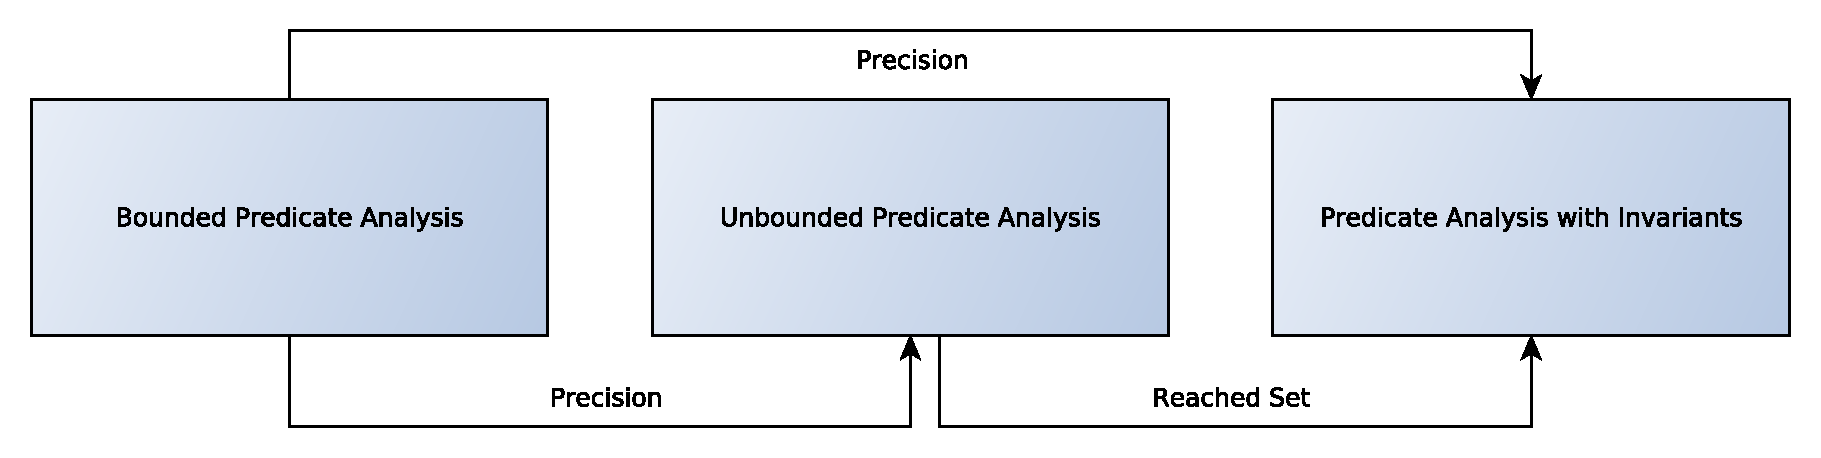
\includegraphics[width=1.20\textwidth]{../../graphics/sequential_invgen}
\end{figure}

\end{adjustwidth}
\end{frame}

\begin{frame}{Auxiliary Invariants --- Parallel Analyses}
 \begin{itemize}
  \item $k$-induction uses concurrently running invariant generation
  \begin{itemize}
  \item[$\lightning$] not usable for other concurrent analyses
  \end{itemize}
  \item[$\rightarrow$] new {\smaller{\textsc{CPAchecker}}} feature
  \item[]
  \item Algorithm for executing several analyses in parallel
  \item Communication between analyses via reached sets
 \end{itemize}
\end{frame}

\begin{frame}{Handling Invariants in the PredicateCPA}
 \begin{itemize}
  \item One manager class
  \begin{itemize}
  \item Exposes general methods for retrieving and generating invariants
  \item Hides exact configuration
  \item Lazy computation of invariants during refinement
  \item Mixing generation and usage strategies possible
  \end{itemize}
  \pause
  \item Two users
  \begin{itemize}
   \item Refinement (precision increment)
   \item PrecisionAdjustment (path -and abstraction formula)
  \end{itemize}
 \end{itemize}
\end{frame}

\section{Evaluation}

\begin{frame}{Evaluation --- Environment}
 \begin{itemize}
  \item \SI{2.6}{\giga\hertz} Octa Core CPUs (Intel E5-2650 v2)
  \item \SI{8}{\giga\byte} memory
  \item \SI{300}{\second} or \SI{600}{\second} CPU time
  \item \emph{trunk} r23084
  \item Measured with {\smaller \textsc{BenchExec}}
  \item[]
  \item 3488 verification tasks taken from SV-COMP'16
 \end{itemize}
\end{frame}

\begin{frame}{Evaluation --- Heuristics}
 \begin{itemize}
  \item Inductive weakening and checking conjuncts of path formulas failed
  \item Checking interpolants on invariance is very slow due to prefix generation
  \item Path invariants are too slow overall, but good on tasks in the loops category
 \end{itemize}
\end{frame}

\begin{frame}{Evaluation --- Path Invariants}
\begin{itemize}
\item Two configurations:
\begin{itemize}
 \item Predicate Analysis + Path Invariants with InvariantsCPA
 \item Predicate Analysis + Path Invariants with PolicyCPA
 \end{itemize}
 %\item[]
 %\item about \SI{4}{\percent} less tasks analyzed correctly overall
 %\item about \SI{40}{\percent} more time consumption for equally and correctly analyzed tasks
 %item about \SI{40}{\percent} successful invariant generation tries
 %item Path Invariants with PolicyCPA are slightly better
\end{itemize}
\begin{adjustwidth}{-3.5em}{-3.5em}
\begin{figure}
 \centering
 \includegraphics[width=1.15\textwidth]{pathInv_diagram.png}
 \end{figure}
 \end{adjustwidth}
\end{frame}

\begin{frame}[fragile]{Evaluation --- Path Invariants}
 \begin{lstlisting}[language=C, frame=single]
 int main() {
    int i;
    for (i = 0; i < 1000000; i++) ;
    assert(i == 1000000);
    return 0;
}
\end{lstlisting}
\begin{itemize}
 \item[$\textcolor{red}{\lightning}$] Interpolation unrolls the loop
 \item[\textcolor{darkgreen}{✓}] found invariant: \texttt{i = 1000000} for location of \texttt{assert} call
\end{itemize}
\end{frame}

\begin{frame}{Evaluation --- Parallel Analyses}
 \begin{itemize}
  \item Combination of:
  \begin{itemize}
  \item An analysis with the PredicateCPA, and
  \item An analysis with the InvariantsCPA (continuously-refined)
 \end{itemize}
 \item \SI{600}{\second} CPU time (\SI{300}{\second} per analysis)
 \item 7 configurations:
 \textbf{abs}, \textbf{prec}, \textbf{path}, \textbf{abs-path}, ...
 \item[]
 \item 3 baselines
 \begin{itemize}
 \item \SI{300}{\second} and \SI{600}{\second} predicate analyses\\
 \textbf{base300}, \textbf{base600}
 \item \SI{600}{\second} parallel analysis without invariant generation\\
 \textbf{basePar}
 \end{itemize}
 \end{itemize}

\end{frame}

\begin{frame}{Evaluation --- Parallel Analyses}
 \begin{figure}
  \centering
\begin{small}
    \begin{tikzpicture}
      \begin{semilogyaxis}[
	  % Which column to be taken from each file
	  /pgfplots/table/y index=3,
	  /pgfplots/table/header=false,
	  % axis labels
	  xlabel=n-th fastest correct result,
	  ylabel=CPU time (\second),
	  % axis ranges
	  xmin= 0,
	  xmax=2150,
	  ymin=2,
	  ymax=650,
	  xtick distance=500,
	  width=\textwidth,
	  height=\textheight,
	  mark repeat=200,
	  cycle list name=exotic,
	  % legend
	  legend entries={base600, base300, basePar, async-abs},
	  every axis legend/.append style={at={(0,1)}, anchor=north west, outer xsep=5pt, outer ysep=5pt,},
	  ]
	  \addplot+[mark phase = 50] table {../../resources/quantile_base_long.csv};
	  \addplot+[mark phase = 120] table {../../resources/quantile_base_short.csv};
	  \addplot+[mark phase = 190] table {../../resources/quantile_base_parallel.csv};
	  \addplot+[mark phase = 260] table {../../resources/quantile_parallel_abs.csv};
      \end{semilogyaxis}
    \end{tikzpicture}
    \end{small}
\end{figure}
\end{frame}

\begin{frame}{Evaluation --- Parallel Analyses}
 \begin{itemize}
  \item all baselines are strictly worse than configurations with invariants
  \item \textbf{async-abs} is the best configuration
  \begin{itemize}
  \item \SI{4}{\percent} better than \textbf{base600}
  \item \SI{8}{\percent} better than \textbf{base300}
  \item \SI{3}{\percent} better than \textbf{basePar}
  \item[$\rightarrow$] wall time is comparable to \textbf{base300}
  \end{itemize}
  
 \item \textbf{async-prec} is slow
 \item \textbf{async-prec-path} almost as good as \textbf{async-abs}
 \end{itemize}

\end{frame}

\begin{frame}{Evaluation --- Sequential Analyses}
  \begin{itemize}
  \item Combination of:
  \begin{itemize}
  \item bounded predicate analysis (\SI{100}{\second})
  \item unbounded predicate analysis without refinement (\SI{100}{\second})
  \item predicate analysis using invariants (\SI{300}{\second})
 \end{itemize}
 \item 7 configurations (invariants):
 \textbf{abs}, \textbf{prec}, \textbf{path}, \textbf{abs-path}, ...
 \item 1 configuration (only precision): \textbf{restart2}
 \item[]
 \item 2 baselines, \SI{300}{\second} and \SI{600}{\second} predicate analyses\\
 \textbf{base300}, \textbf{base600}
 \end{itemize}
\end{frame}

\begin{frame}{Evaluation --- Sequential Analyses}
\begin{adjustwidth}{-3.5em}{-3.5em}
\begin{figure}
 \centering
 \includegraphics[width=1.15\textwidth]{restart_diagram.png}
 \end{figure}
 \end{adjustwidth}
\end{frame}

\begin{frame}{Conclusion \& Outlook}
  \begin{itemize}
    \item Heuristics for invariant generation need more time than expected
    \item More intelligent heuristics needed:
    \begin{itemize}
    \item When should invariants be generated
    \item Filtering of found invariants
    \end{itemize}
    \pause
    \item[]
    \item[\textcolor{darkgreen}{✓}] Combination of analyses increases performance
    \item[\textcolor{darkgreen}{✓}] Performance is even better if the analyses communicate
    \item[$\rightarrow$] Aim: Make communication easier usable
  \end{itemize}
\end{frame}

\appendix
\backupbegin
\begin{frame}{Path Invariants --- Table (1)}
 %%% predicate_bitprecise_pathinvariants.2016-09-10_1338.results.pathInvariants-invCPA %%%
 %% correct %%
\providecommand{\predicateBitprecisePathinvariantsResultsPathInvariantsInvCPACorrectPlain}{}
  \renewcommand{\predicateBitprecisePathinvariantsResultsPathInvariantsInvCPACorrectPlain}{1846\xspace}

  % cpu-time-sum
\providecommand{\predicateBitprecisePathinvariantsResultsPathInvariantsInvCPACorrectCpuTimeSumPlain}{}
  \renewcommand{\predicateBitprecisePathinvariantsResultsPathInvariantsInvCPACorrectCpuTimeSumPlain}{111598.89775255592\xspace}
\providecommand{\predicateBitprecisePathinvariantsResultsPathInvariantsInvCPACorrectCpuTimeSumPlainHours}{}
  \renewcommand{\predicateBitprecisePathinvariantsResultsPathInvariantsInvCPACorrectCpuTimeSumPlainHours}{30.99969382015442\xspace}

  % wall-time-sum
\providecommand{\predicateBitprecisePathinvariantsResultsPathInvariantsInvCPACorrectWallTimeSumPlain}{}
  \renewcommand{\predicateBitprecisePathinvariantsResultsPathInvariantsInvCPACorrectWallTimeSumPlain}{62256.46204423421\xspace}
\providecommand{\predicateBitprecisePathinvariantsResultsPathInvariantsInvCPACorrectWallTimeSumPlainHours}{}
  \renewcommand{\predicateBitprecisePathinvariantsResultsPathInvariantsInvCPACorrectWallTimeSumPlainHours}{17.29346167895395\xspace}

  % cpu-time-avg
\providecommand{\predicateBitprecisePathinvariantsResultsPathInvariantsInvCPACorrectCpuTimeAvgPlain}{}
  \renewcommand{\predicateBitprecisePathinvariantsResultsPathInvariantsInvCPACorrectCpuTimeAvgPlain}{60.4544408193694\xspace}
\providecommand{\predicateBitprecisePathinvariantsResultsPathInvariantsInvCPACorrectCpuTimeAvgPlainHours}{}
  \renewcommand{\predicateBitprecisePathinvariantsResultsPathInvariantsInvCPACorrectCpuTimeAvgPlainHours}{0.016792900227602613\xspace}

  % wall-time-avg
\providecommand{\predicateBitprecisePathinvariantsResultsPathInvariantsInvCPACorrectWallTimeAvgPlain}{}
  \renewcommand{\predicateBitprecisePathinvariantsResultsPathInvariantsInvCPACorrectWallTimeAvgPlain}{33.72506069568484\xspace}
\providecommand{\predicateBitprecisePathinvariantsResultsPathInvariantsInvCPACorrectWallTimeAvgPlainHours}{}
  \renewcommand{\predicateBitprecisePathinvariantsResultsPathInvariantsInvCPACorrectWallTimeAvgPlainHours}{0.00936807241546801\xspace}

  % inv-succ
\providecommand{\predicateBitprecisePathinvariantsResultsPathInvariantsInvCPACorrectInvSuccPlain}{}
  \renewcommand{\predicateBitprecisePathinvariantsResultsPathInvariantsInvCPACorrectInvSuccPlain}{1428\xspace}

  % inv-tries
\providecommand{\predicateBitprecisePathinvariantsResultsPathInvariantsInvCPACorrectInvTriesPlain}{}
  \renewcommand{\predicateBitprecisePathinvariantsResultsPathInvariantsInvCPACorrectInvTriesPlain}{4719\xspace}

  % inv-time-sum
\providecommand{\predicateBitprecisePathinvariantsResultsPathInvariantsInvCPACorrectInvTimeSumPlain}{}
  \renewcommand{\predicateBitprecisePathinvariantsResultsPathInvariantsInvCPACorrectInvTimeSumPlain}{8484.282000000007\xspace}
\providecommand{\predicateBitprecisePathinvariantsResultsPathInvariantsInvCPACorrectInvTimeSumPlainHours}{}
  \renewcommand{\predicateBitprecisePathinvariantsResultsPathInvariantsInvCPACorrectInvTimeSumPlainHours}{2.356745000000002\xspace}

 %% incorrect %%
\providecommand{\predicateBitprecisePathinvariantsResultsPathInvariantsInvCPAIncorrectPlain}{}
  \renewcommand{\predicateBitprecisePathinvariantsResultsPathInvariantsInvCPAIncorrectPlain}{27\xspace}

  % cpu-time-sum
\providecommand{\predicateBitprecisePathinvariantsResultsPathInvariantsInvCPAIncorrectCpuTimeSumPlain}{}
  \renewcommand{\predicateBitprecisePathinvariantsResultsPathInvariantsInvCPAIncorrectCpuTimeSumPlain}{1183.27833542\xspace}
\providecommand{\predicateBitprecisePathinvariantsResultsPathInvariantsInvCPAIncorrectCpuTimeSumPlainHours}{}
  \renewcommand{\predicateBitprecisePathinvariantsResultsPathInvariantsInvCPAIncorrectCpuTimeSumPlainHours}{0.3286884265055556\xspace}

  % wall-time-sum
\providecommand{\predicateBitprecisePathinvariantsResultsPathInvariantsInvCPAIncorrectWallTimeSumPlain}{}
  \renewcommand{\predicateBitprecisePathinvariantsResultsPathInvariantsInvCPAIncorrectWallTimeSumPlain}{566.5751395224701\xspace}
\providecommand{\predicateBitprecisePathinvariantsResultsPathInvariantsInvCPAIncorrectWallTimeSumPlainHours}{}
  \renewcommand{\predicateBitprecisePathinvariantsResultsPathInvariantsInvCPAIncorrectWallTimeSumPlainHours}{0.15738198320068614\xspace}

  % cpu-time-avg
\providecommand{\predicateBitprecisePathinvariantsResultsPathInvariantsInvCPAIncorrectCpuTimeAvgPlain}{}
  \renewcommand{\predicateBitprecisePathinvariantsResultsPathInvariantsInvCPAIncorrectCpuTimeAvgPlain}{43.82512353407407\xspace}
\providecommand{\predicateBitprecisePathinvariantsResultsPathInvariantsInvCPAIncorrectCpuTimeAvgPlainHours}{}
  \renewcommand{\predicateBitprecisePathinvariantsResultsPathInvariantsInvCPAIncorrectCpuTimeAvgPlainHours}{0.012173645426131688\xspace}

  % wall-time-avg
\providecommand{\predicateBitprecisePathinvariantsResultsPathInvariantsInvCPAIncorrectWallTimeAvgPlain}{}
  \renewcommand{\predicateBitprecisePathinvariantsResultsPathInvariantsInvCPAIncorrectWallTimeAvgPlain}{20.984264426758152\xspace}
\providecommand{\predicateBitprecisePathinvariantsResultsPathInvariantsInvCPAIncorrectWallTimeAvgPlainHours}{}
  \renewcommand{\predicateBitprecisePathinvariantsResultsPathInvariantsInvCPAIncorrectWallTimeAvgPlainHours}{0.005828962340766153\xspace}

  % inv-succ
\providecommand{\predicateBitprecisePathinvariantsResultsPathInvariantsInvCPAIncorrectInvSuccPlain}{}
  \renewcommand{\predicateBitprecisePathinvariantsResultsPathInvariantsInvCPAIncorrectInvSuccPlain}{3\xspace}

  % inv-tries
\providecommand{\predicateBitprecisePathinvariantsResultsPathInvariantsInvCPAIncorrectInvTriesPlain}{}
  \renewcommand{\predicateBitprecisePathinvariantsResultsPathInvariantsInvCPAIncorrectInvTriesPlain}{60\xspace}

  % inv-time-sum
\providecommand{\predicateBitprecisePathinvariantsResultsPathInvariantsInvCPAIncorrectInvTimeSumPlain}{}
  \renewcommand{\predicateBitprecisePathinvariantsResultsPathInvariantsInvCPAIncorrectInvTimeSumPlain}{119.849\xspace}
\providecommand{\predicateBitprecisePathinvariantsResultsPathInvariantsInvCPAIncorrectInvTimeSumPlainHours}{}
  \renewcommand{\predicateBitprecisePathinvariantsResultsPathInvariantsInvCPAIncorrectInvTimeSumPlainHours}{0.03329138888888889\xspace}

 %% timeout %%
\providecommand{\predicateBitprecisePathinvariantsResultsPathInvariantsInvCPATimeoutPlain}{}
  \renewcommand{\predicateBitprecisePathinvariantsResultsPathInvariantsInvCPATimeoutPlain}{1499\xspace}

  % cpu-time-sum
\providecommand{\predicateBitprecisePathinvariantsResultsPathInvariantsInvCPATimeoutCpuTimeSumPlain}{}
  \renewcommand{\predicateBitprecisePathinvariantsResultsPathInvariantsInvCPATimeoutCpuTimeSumPlain}{458267.74822316313\xspace}
\providecommand{\predicateBitprecisePathinvariantsResultsPathInvariantsInvCPATimeoutCpuTimeSumPlainHours}{}
  \renewcommand{\predicateBitprecisePathinvariantsResultsPathInvariantsInvCPATimeoutCpuTimeSumPlainHours}{127.29659672865643\xspace}

  % wall-time-sum
\providecommand{\predicateBitprecisePathinvariantsResultsPathInvariantsInvCPATimeoutWallTimeSumPlain}{}
  \renewcommand{\predicateBitprecisePathinvariantsResultsPathInvariantsInvCPATimeoutWallTimeSumPlain}{385266.7221231276\xspace}
\providecommand{\predicateBitprecisePathinvariantsResultsPathInvariantsInvCPATimeoutWallTimeSumPlainHours}{}
  \renewcommand{\predicateBitprecisePathinvariantsResultsPathInvariantsInvCPATimeoutWallTimeSumPlainHours}{107.018533923091\xspace}

  % cpu-time-avg
\providecommand{\predicateBitprecisePathinvariantsResultsPathInvariantsInvCPATimeoutCpuTimeAvgPlain}{}
  \renewcommand{\predicateBitprecisePathinvariantsResultsPathInvariantsInvCPATimeoutCpuTimeAvgPlain}{305.71564257716017\xspace}
\providecommand{\predicateBitprecisePathinvariantsResultsPathInvariantsInvCPATimeoutCpuTimeAvgPlainHours}{}
  \renewcommand{\predicateBitprecisePathinvariantsResultsPathInvariantsInvCPATimeoutCpuTimeAvgPlainHours}{0.08492101182698894\xspace}

  % wall-time-avg
\providecommand{\predicateBitprecisePathinvariantsResultsPathInvariantsInvCPATimeoutWallTimeAvgPlain}{}
  \renewcommand{\predicateBitprecisePathinvariantsResultsPathInvariantsInvCPATimeoutWallTimeAvgPlain}{257.01582529895103\xspace}
\providecommand{\predicateBitprecisePathinvariantsResultsPathInvariantsInvCPATimeoutWallTimeAvgPlainHours}{}
  \renewcommand{\predicateBitprecisePathinvariantsResultsPathInvariantsInvCPATimeoutWallTimeAvgPlainHours}{0.07139328480526418\xspace}

  % inv-succ
\providecommand{\predicateBitprecisePathinvariantsResultsPathInvariantsInvCPATimeoutInvSuccPlain}{}
  \renewcommand{\predicateBitprecisePathinvariantsResultsPathInvariantsInvCPATimeoutInvSuccPlain}{53883\xspace}

  % inv-tries
\providecommand{\predicateBitprecisePathinvariantsResultsPathInvariantsInvCPATimeoutInvTriesPlain}{}
  \renewcommand{\predicateBitprecisePathinvariantsResultsPathInvariantsInvCPATimeoutInvTriesPlain}{61094\xspace}

  % inv-time-sum
\providecommand{\predicateBitprecisePathinvariantsResultsPathInvariantsInvCPATimeoutInvTimeSumPlain}{}
  \renewcommand{\predicateBitprecisePathinvariantsResultsPathInvariantsInvCPATimeoutInvTimeSumPlain}{14506.15700000001\xspace}
\providecommand{\predicateBitprecisePathinvariantsResultsPathInvariantsInvCPATimeoutInvTimeSumPlainHours}{}
  \renewcommand{\predicateBitprecisePathinvariantsResultsPathInvariantsInvCPATimeoutInvTimeSumPlainHours}{4.029488055555558\xspace}

 %% unknown-or-category-error %%
\providecommand{\predicateBitprecisePathinvariantsResultsPathInvariantsInvCPAUnknownOrCategoryErrorPlain}{}
  \renewcommand{\predicateBitprecisePathinvariantsResultsPathInvariantsInvCPAUnknownOrCategoryErrorPlain}{1615\xspace}

  % cpu-time-sum
\providecommand{\predicateBitprecisePathinvariantsResultsPathInvariantsInvCPAUnknownOrCategoryErrorCpuTimeSumPlain}{}
  \renewcommand{\predicateBitprecisePathinvariantsResultsPathInvariantsInvCPAUnknownOrCategoryErrorCpuTimeSumPlain}{471990.4606770793\xspace}
\providecommand{\predicateBitprecisePathinvariantsResultsPathInvariantsInvCPAUnknownOrCategoryErrorCpuTimeSumPlainHours}{}
  \renewcommand{\predicateBitprecisePathinvariantsResultsPathInvariantsInvCPAUnknownOrCategoryErrorCpuTimeSumPlainHours}{131.1084612991887\xspace}

  % wall-time-sum
\providecommand{\predicateBitprecisePathinvariantsResultsPathInvariantsInvCPAUnknownOrCategoryErrorWallTimeSumPlain}{}
  \renewcommand{\predicateBitprecisePathinvariantsResultsPathInvariantsInvCPAUnknownOrCategoryErrorWallTimeSumPlain}{394047.456606367\xspace}
\providecommand{\predicateBitprecisePathinvariantsResultsPathInvariantsInvCPAUnknownOrCategoryErrorWallTimeSumPlainHours}{}
  \renewcommand{\predicateBitprecisePathinvariantsResultsPathInvariantsInvCPAUnknownOrCategoryErrorWallTimeSumPlainHours}{109.45762683510195\xspace}

  % cpu-time-avg
\providecommand{\predicateBitprecisePathinvariantsResultsPathInvariantsInvCPAUnknownOrCategoryErrorCpuTimeAvgPlain}{}
  \renewcommand{\predicateBitprecisePathinvariantsResultsPathInvariantsInvCPAUnknownOrCategoryErrorCpuTimeAvgPlain}{292.25415521800574\xspace}
\providecommand{\predicateBitprecisePathinvariantsResultsPathInvariantsInvCPAUnknownOrCategoryErrorCpuTimeAvgPlainHours}{}
  \renewcommand{\predicateBitprecisePathinvariantsResultsPathInvariantsInvCPAUnknownOrCategoryErrorCpuTimeAvgPlainHours}{0.08118170978277937\xspace}

  % wall-time-avg
\providecommand{\predicateBitprecisePathinvariantsResultsPathInvariantsInvCPAUnknownOrCategoryErrorWallTimeAvgPlain}{}
  \renewcommand{\predicateBitprecisePathinvariantsResultsPathInvariantsInvCPAUnknownOrCategoryErrorWallTimeAvgPlain}{243.99223319279693\xspace}
\providecommand{\predicateBitprecisePathinvariantsResultsPathInvariantsInvCPAUnknownOrCategoryErrorWallTimeAvgPlainHours}{}
  \renewcommand{\predicateBitprecisePathinvariantsResultsPathInvariantsInvCPAUnknownOrCategoryErrorWallTimeAvgPlainHours}{0.06777562033133248\xspace}

  % inv-succ
\providecommand{\predicateBitprecisePathinvariantsResultsPathInvariantsInvCPAUnknownOrCategoryErrorInvSuccPlain}{}
  \renewcommand{\predicateBitprecisePathinvariantsResultsPathInvariantsInvCPAUnknownOrCategoryErrorInvSuccPlain}{53883\xspace}

  % inv-tries
\providecommand{\predicateBitprecisePathinvariantsResultsPathInvariantsInvCPAUnknownOrCategoryErrorInvTriesPlain}{}
  \renewcommand{\predicateBitprecisePathinvariantsResultsPathInvariantsInvCPAUnknownOrCategoryErrorInvTriesPlain}{61437\xspace}

  % inv-time-sum
\providecommand{\predicateBitprecisePathinvariantsResultsPathInvariantsInvCPAUnknownOrCategoryErrorInvTimeSumPlain}{}
  \renewcommand{\predicateBitprecisePathinvariantsResultsPathInvariantsInvCPAUnknownOrCategoryErrorInvTimeSumPlain}{15480.154000000013\xspace}
\providecommand{\predicateBitprecisePathinvariantsResultsPathInvariantsInvCPAUnknownOrCategoryErrorInvTimeSumPlainHours}{}
  \renewcommand{\predicateBitprecisePathinvariantsResultsPathInvariantsInvCPAUnknownOrCategoryErrorInvTimeSumPlainHours}{4.300042777777781\xspace}

 %% correct-false %%
\providecommand{\predicateBitprecisePathinvariantsResultsPathInvariantsInvCPACorrectFalsePlain}{}
  \renewcommand{\predicateBitprecisePathinvariantsResultsPathInvariantsInvCPACorrectFalsePlain}{519\xspace}

  % cpu-time-sum
\providecommand{\predicateBitprecisePathinvariantsResultsPathInvariantsInvCPACorrectFalseCpuTimeSumPlain}{}
  \renewcommand{\predicateBitprecisePathinvariantsResultsPathInvariantsInvCPACorrectFalseCpuTimeSumPlain}{37347.92062543605\xspace}
\providecommand{\predicateBitprecisePathinvariantsResultsPathInvariantsInvCPACorrectFalseCpuTimeSumPlainHours}{}
  \renewcommand{\predicateBitprecisePathinvariantsResultsPathInvariantsInvCPACorrectFalseCpuTimeSumPlainHours}{10.374422395954458\xspace}

  % wall-time-sum
\providecommand{\predicateBitprecisePathinvariantsResultsPathInvariantsInvCPACorrectFalseWallTimeSumPlain}{}
  \renewcommand{\predicateBitprecisePathinvariantsResultsPathInvariantsInvCPACorrectFalseWallTimeSumPlain}{23382.190789456225\xspace}
\providecommand{\predicateBitprecisePathinvariantsResultsPathInvariantsInvCPACorrectFalseWallTimeSumPlainHours}{}
  \renewcommand{\predicateBitprecisePathinvariantsResultsPathInvariantsInvCPACorrectFalseWallTimeSumPlainHours}{6.4950529970711735\xspace}

  % cpu-time-avg
\providecommand{\predicateBitprecisePathinvariantsResultsPathInvariantsInvCPACorrectFalseCpuTimeAvgPlain}{}
  \renewcommand{\predicateBitprecisePathinvariantsResultsPathInvariantsInvCPACorrectFalseCpuTimeAvgPlain}{71.96131141702514\xspace}
\providecommand{\predicateBitprecisePathinvariantsResultsPathInvariantsInvCPACorrectFalseCpuTimeAvgPlainHours}{}
  \renewcommand{\predicateBitprecisePathinvariantsResultsPathInvariantsInvCPACorrectFalseCpuTimeAvgPlainHours}{0.01998925317139587\xspace}

  % wall-time-avg
\providecommand{\predicateBitprecisePathinvariantsResultsPathInvariantsInvCPACorrectFalseWallTimeAvgPlain}{}
  \renewcommand{\predicateBitprecisePathinvariantsResultsPathInvariantsInvCPACorrectFalseWallTimeAvgPlain}{45.05239073112953\xspace}
\providecommand{\predicateBitprecisePathinvariantsResultsPathInvariantsInvCPACorrectFalseWallTimeAvgPlainHours}{}
  \renewcommand{\predicateBitprecisePathinvariantsResultsPathInvariantsInvCPACorrectFalseWallTimeAvgPlainHours}{0.012514552980869313\xspace}

  % inv-succ
\providecommand{\predicateBitprecisePathinvariantsResultsPathInvariantsInvCPACorrectFalseInvSuccPlain}{}
  \renewcommand{\predicateBitprecisePathinvariantsResultsPathInvariantsInvCPACorrectFalseInvSuccPlain}{455\xspace}

  % inv-tries
\providecommand{\predicateBitprecisePathinvariantsResultsPathInvariantsInvCPACorrectFalseInvTriesPlain}{}
  \renewcommand{\predicateBitprecisePathinvariantsResultsPathInvariantsInvCPACorrectFalseInvTriesPlain}{1489\xspace}

  % inv-time-sum
\providecommand{\predicateBitprecisePathinvariantsResultsPathInvariantsInvCPACorrectFalseInvTimeSumPlain}{}
  \renewcommand{\predicateBitprecisePathinvariantsResultsPathInvariantsInvCPACorrectFalseInvTimeSumPlain}{2068.579000000002\xspace}
\providecommand{\predicateBitprecisePathinvariantsResultsPathInvariantsInvCPACorrectFalseInvTimeSumPlainHours}{}
  \renewcommand{\predicateBitprecisePathinvariantsResultsPathInvariantsInvCPACorrectFalseInvTimeSumPlainHours}{0.5746052777777784\xspace}

 %% correct-true %%
\providecommand{\predicateBitprecisePathinvariantsResultsPathInvariantsInvCPACorrectTruePlain}{}
  \renewcommand{\predicateBitprecisePathinvariantsResultsPathInvariantsInvCPACorrectTruePlain}{1327\xspace}

  % cpu-time-sum
\providecommand{\predicateBitprecisePathinvariantsResultsPathInvariantsInvCPACorrectTrueCpuTimeSumPlain}{}
  \renewcommand{\predicateBitprecisePathinvariantsResultsPathInvariantsInvCPACorrectTrueCpuTimeSumPlain}{74250.97712712\xspace}
\providecommand{\predicateBitprecisePathinvariantsResultsPathInvariantsInvCPACorrectTrueCpuTimeSumPlainHours}{}
  \renewcommand{\predicateBitprecisePathinvariantsResultsPathInvariantsInvCPACorrectTrueCpuTimeSumPlainHours}{20.6252714242\xspace}

  % wall-time-sum
\providecommand{\predicateBitprecisePathinvariantsResultsPathInvariantsInvCPACorrectTrueWallTimeSumPlain}{}
  \renewcommand{\predicateBitprecisePathinvariantsResultsPathInvariantsInvCPACorrectTrueWallTimeSumPlain}{38874.27125477804\xspace}
\providecommand{\predicateBitprecisePathinvariantsResultsPathInvariantsInvCPACorrectTrueWallTimeSumPlainHours}{}
  \renewcommand{\predicateBitprecisePathinvariantsResultsPathInvariantsInvCPACorrectTrueWallTimeSumPlainHours}{10.798408681882789\xspace}

  % cpu-time-avg
\providecommand{\predicateBitprecisePathinvariantsResultsPathInvariantsInvCPACorrectTrueCpuTimeAvgPlain}{}
  \renewcommand{\predicateBitprecisePathinvariantsResultsPathInvariantsInvCPACorrectTrueCpuTimeAvgPlain}{55.954014413805574\xspace}
\providecommand{\predicateBitprecisePathinvariantsResultsPathInvariantsInvCPACorrectTrueCpuTimeAvgPlainHours}{}
  \renewcommand{\predicateBitprecisePathinvariantsResultsPathInvariantsInvCPACorrectTrueCpuTimeAvgPlainHours}{0.015542781781612659\xspace}

  % wall-time-avg
\providecommand{\predicateBitprecisePathinvariantsResultsPathInvariantsInvCPACorrectTrueWallTimeAvgPlain}{}
  \renewcommand{\predicateBitprecisePathinvariantsResultsPathInvariantsInvCPACorrectTrueWallTimeAvgPlain}{29.294853997571998\xspace}
\providecommand{\predicateBitprecisePathinvariantsResultsPathInvariantsInvCPACorrectTrueWallTimeAvgPlainHours}{}
  \renewcommand{\predicateBitprecisePathinvariantsResultsPathInvariantsInvCPACorrectTrueWallTimeAvgPlainHours}{0.00813745944377\xspace}

  % inv-succ
\providecommand{\predicateBitprecisePathinvariantsResultsPathInvariantsInvCPACorrectTrueInvSuccPlain}{}
  \renewcommand{\predicateBitprecisePathinvariantsResultsPathInvariantsInvCPACorrectTrueInvSuccPlain}{973\xspace}

  % inv-tries
\providecommand{\predicateBitprecisePathinvariantsResultsPathInvariantsInvCPACorrectTrueInvTriesPlain}{}
  \renewcommand{\predicateBitprecisePathinvariantsResultsPathInvariantsInvCPACorrectTrueInvTriesPlain}{3230\xspace}

  % inv-time-sum
\providecommand{\predicateBitprecisePathinvariantsResultsPathInvariantsInvCPACorrectTrueInvTimeSumPlain}{}
  \renewcommand{\predicateBitprecisePathinvariantsResultsPathInvariantsInvCPACorrectTrueInvTimeSumPlain}{6415.702999999995\xspace}
\providecommand{\predicateBitprecisePathinvariantsResultsPathInvariantsInvCPACorrectTrueInvTimeSumPlainHours}{}
  \renewcommand{\predicateBitprecisePathinvariantsResultsPathInvariantsInvCPACorrectTrueInvTimeSumPlainHours}{1.7821397222222208\xspace}

 %% incorrect-false %%
\providecommand{\predicateBitprecisePathinvariantsResultsPathInvariantsInvCPAIncorrectFalsePlain}{}
  \renewcommand{\predicateBitprecisePathinvariantsResultsPathInvariantsInvCPAIncorrectFalsePlain}{27\xspace}

  % cpu-time-sum
\providecommand{\predicateBitprecisePathinvariantsResultsPathInvariantsInvCPAIncorrectFalseCpuTimeSumPlain}{}
  \renewcommand{\predicateBitprecisePathinvariantsResultsPathInvariantsInvCPAIncorrectFalseCpuTimeSumPlain}{1183.27833542\xspace}
\providecommand{\predicateBitprecisePathinvariantsResultsPathInvariantsInvCPAIncorrectFalseCpuTimeSumPlainHours}{}
  \renewcommand{\predicateBitprecisePathinvariantsResultsPathInvariantsInvCPAIncorrectFalseCpuTimeSumPlainHours}{0.3286884265055556\xspace}

  % wall-time-sum
\providecommand{\predicateBitprecisePathinvariantsResultsPathInvariantsInvCPAIncorrectFalseWallTimeSumPlain}{}
  \renewcommand{\predicateBitprecisePathinvariantsResultsPathInvariantsInvCPAIncorrectFalseWallTimeSumPlain}{566.5751395224701\xspace}
\providecommand{\predicateBitprecisePathinvariantsResultsPathInvariantsInvCPAIncorrectFalseWallTimeSumPlainHours}{}
  \renewcommand{\predicateBitprecisePathinvariantsResultsPathInvariantsInvCPAIncorrectFalseWallTimeSumPlainHours}{0.15738198320068614\xspace}

  % cpu-time-avg
\providecommand{\predicateBitprecisePathinvariantsResultsPathInvariantsInvCPAIncorrectFalseCpuTimeAvgPlain}{}
  \renewcommand{\predicateBitprecisePathinvariantsResultsPathInvariantsInvCPAIncorrectFalseCpuTimeAvgPlain}{43.82512353407407\xspace}
\providecommand{\predicateBitprecisePathinvariantsResultsPathInvariantsInvCPAIncorrectFalseCpuTimeAvgPlainHours}{}
  \renewcommand{\predicateBitprecisePathinvariantsResultsPathInvariantsInvCPAIncorrectFalseCpuTimeAvgPlainHours}{0.012173645426131688\xspace}

  % wall-time-avg
\providecommand{\predicateBitprecisePathinvariantsResultsPathInvariantsInvCPAIncorrectFalseWallTimeAvgPlain}{}
  \renewcommand{\predicateBitprecisePathinvariantsResultsPathInvariantsInvCPAIncorrectFalseWallTimeAvgPlain}{20.984264426758152\xspace}
\providecommand{\predicateBitprecisePathinvariantsResultsPathInvariantsInvCPAIncorrectFalseWallTimeAvgPlainHours}{}
  \renewcommand{\predicateBitprecisePathinvariantsResultsPathInvariantsInvCPAIncorrectFalseWallTimeAvgPlainHours}{0.005828962340766153\xspace}

  % inv-succ
\providecommand{\predicateBitprecisePathinvariantsResultsPathInvariantsInvCPAIncorrectFalseInvSuccPlain}{}
  \renewcommand{\predicateBitprecisePathinvariantsResultsPathInvariantsInvCPAIncorrectFalseInvSuccPlain}{3\xspace}

  % inv-tries
\providecommand{\predicateBitprecisePathinvariantsResultsPathInvariantsInvCPAIncorrectFalseInvTriesPlain}{}
  \renewcommand{\predicateBitprecisePathinvariantsResultsPathInvariantsInvCPAIncorrectFalseInvTriesPlain}{60\xspace}

  % inv-time-sum
\providecommand{\predicateBitprecisePathinvariantsResultsPathInvariantsInvCPAIncorrectFalseInvTimeSumPlain}{}
  \renewcommand{\predicateBitprecisePathinvariantsResultsPathInvariantsInvCPAIncorrectFalseInvTimeSumPlain}{119.849\xspace}
\providecommand{\predicateBitprecisePathinvariantsResultsPathInvariantsInvCPAIncorrectFalseInvTimeSumPlainHours}{}
  \renewcommand{\predicateBitprecisePathinvariantsResultsPathInvariantsInvCPAIncorrectFalseInvTimeSumPlainHours}{0.03329138888888889\xspace}

 %% incorrect-true %%
\providecommand{\predicateBitprecisePathinvariantsResultsPathInvariantsInvCPAIncorrectTruePlain}{}
  \renewcommand{\predicateBitprecisePathinvariantsResultsPathInvariantsInvCPAIncorrectTruePlain}{0\xspace}

  % cpu-time-sum
\providecommand{\predicateBitprecisePathinvariantsResultsPathInvariantsInvCPAIncorrectTrueCpuTimeSumPlain}{}
  \renewcommand{\predicateBitprecisePathinvariantsResultsPathInvariantsInvCPAIncorrectTrueCpuTimeSumPlain}{0.0\xspace}
\providecommand{\predicateBitprecisePathinvariantsResultsPathInvariantsInvCPAIncorrectTrueCpuTimeSumPlainHours}{}
  \renewcommand{\predicateBitprecisePathinvariantsResultsPathInvariantsInvCPAIncorrectTrueCpuTimeSumPlainHours}{0.0\xspace}

  % wall-time-sum
\providecommand{\predicateBitprecisePathinvariantsResultsPathInvariantsInvCPAIncorrectTrueWallTimeSumPlain}{}
  \renewcommand{\predicateBitprecisePathinvariantsResultsPathInvariantsInvCPAIncorrectTrueWallTimeSumPlain}{0.0\xspace}
\providecommand{\predicateBitprecisePathinvariantsResultsPathInvariantsInvCPAIncorrectTrueWallTimeSumPlainHours}{}
  \renewcommand{\predicateBitprecisePathinvariantsResultsPathInvariantsInvCPAIncorrectTrueWallTimeSumPlainHours}{0.0\xspace}

  % cpu-time-avg
\providecommand{\predicateBitprecisePathinvariantsResultsPathInvariantsInvCPAIncorrectTrueCpuTimeAvgPlain}{}
  \renewcommand{\predicateBitprecisePathinvariantsResultsPathInvariantsInvCPAIncorrectTrueCpuTimeAvgPlain}{NaN\xspace}
\providecommand{\predicateBitprecisePathinvariantsResultsPathInvariantsInvCPAIncorrectTrueCpuTimeAvgPlainHours}{}
  \renewcommand{\predicateBitprecisePathinvariantsResultsPathInvariantsInvCPAIncorrectTrueCpuTimeAvgPlainHours}{NaN\xspace}

  % wall-time-avg
\providecommand{\predicateBitprecisePathinvariantsResultsPathInvariantsInvCPAIncorrectTrueWallTimeAvgPlain}{}
  \renewcommand{\predicateBitprecisePathinvariantsResultsPathInvariantsInvCPAIncorrectTrueWallTimeAvgPlain}{NaN\xspace}
\providecommand{\predicateBitprecisePathinvariantsResultsPathInvariantsInvCPAIncorrectTrueWallTimeAvgPlainHours}{}
  \renewcommand{\predicateBitprecisePathinvariantsResultsPathInvariantsInvCPAIncorrectTrueWallTimeAvgPlainHours}{NaN\xspace}

  % inv-succ
\providecommand{\predicateBitprecisePathinvariantsResultsPathInvariantsInvCPAIncorrectTrueInvSuccPlain}{}
  \renewcommand{\predicateBitprecisePathinvariantsResultsPathInvariantsInvCPAIncorrectTrueInvSuccPlain}{0\xspace}

  % inv-tries
\providecommand{\predicateBitprecisePathinvariantsResultsPathInvariantsInvCPAIncorrectTrueInvTriesPlain}{}
  \renewcommand{\predicateBitprecisePathinvariantsResultsPathInvariantsInvCPAIncorrectTrueInvTriesPlain}{0\xspace}

  % inv-time-sum
\providecommand{\predicateBitprecisePathinvariantsResultsPathInvariantsInvCPAIncorrectTrueInvTimeSumPlain}{}
  \renewcommand{\predicateBitprecisePathinvariantsResultsPathInvariantsInvCPAIncorrectTrueInvTimeSumPlain}{0.0\xspace}
\providecommand{\predicateBitprecisePathinvariantsResultsPathInvariantsInvCPAIncorrectTrueInvTimeSumPlainHours}{}
  \renewcommand{\predicateBitprecisePathinvariantsResultsPathInvariantsInvCPAIncorrectTrueInvTimeSumPlainHours}{0.0\xspace}

 %% all %%
\providecommand{\predicateBitprecisePathinvariantsResultsPathInvariantsInvCPAAllPlain}{}
  \renewcommand{\predicateBitprecisePathinvariantsResultsPathInvariantsInvCPAAllPlain}{3488\xspace}

  % cpu-time-sum
\providecommand{\predicateBitprecisePathinvariantsResultsPathInvariantsInvCPAAllCpuTimeSumPlain}{}
  \renewcommand{\predicateBitprecisePathinvariantsResultsPathInvariantsInvCPAAllCpuTimeSumPlain}{584772.6367650569\xspace}
\providecommand{\predicateBitprecisePathinvariantsResultsPathInvariantsInvCPAAllCpuTimeSumPlainHours}{}
  \renewcommand{\predicateBitprecisePathinvariantsResultsPathInvariantsInvCPAAllCpuTimeSumPlainHours}{162.43684354584914\xspace}

  % wall-time-sum
\providecommand{\predicateBitprecisePathinvariantsResultsPathInvariantsInvCPAAllWallTimeSumPlain}{}
  \renewcommand{\predicateBitprecisePathinvariantsResultsPathInvariantsInvCPAAllWallTimeSumPlain}{456870.49379012437\xspace}
\providecommand{\predicateBitprecisePathinvariantsResultsPathInvariantsInvCPAAllWallTimeSumPlainHours}{}
  \renewcommand{\predicateBitprecisePathinvariantsResultsPathInvariantsInvCPAAllWallTimeSumPlainHours}{126.90847049725677\xspace}

  % cpu-time-avg
\providecommand{\predicateBitprecisePathinvariantsResultsPathInvariantsInvCPAAllCpuTimeAvgPlain}{}
  \renewcommand{\predicateBitprecisePathinvariantsResultsPathInvariantsInvCPAAllCpuTimeAvgPlain}{167.65270549456906\xspace}
\providecommand{\predicateBitprecisePathinvariantsResultsPathInvariantsInvCPAAllCpuTimeAvgPlainHours}{}
  \renewcommand{\predicateBitprecisePathinvariantsResultsPathInvariantsInvCPAAllCpuTimeAvgPlainHours}{0.04657019597071363\xspace}

  % wall-time-avg
\providecommand{\predicateBitprecisePathinvariantsResultsPathInvariantsInvCPAAllWallTimeAvgPlain}{}
  \renewcommand{\predicateBitprecisePathinvariantsResultsPathInvariantsInvCPAAllWallTimeAvgPlain}{130.98351312790263\xspace}
\providecommand{\predicateBitprecisePathinvariantsResultsPathInvariantsInvCPAAllWallTimeAvgPlainHours}{}
  \renewcommand{\predicateBitprecisePathinvariantsResultsPathInvariantsInvCPAAllWallTimeAvgPlainHours}{0.036384309202195174\xspace}

  % inv-succ
\providecommand{\predicateBitprecisePathinvariantsResultsPathInvariantsInvCPAAllInvSuccPlain}{}
  \renewcommand{\predicateBitprecisePathinvariantsResultsPathInvariantsInvCPAAllInvSuccPlain}{55314\xspace}

  % inv-tries
\providecommand{\predicateBitprecisePathinvariantsResultsPathInvariantsInvCPAAllInvTriesPlain}{}
  \renewcommand{\predicateBitprecisePathinvariantsResultsPathInvariantsInvCPAAllInvTriesPlain}{66216\xspace}

  % inv-time-sum
\providecommand{\predicateBitprecisePathinvariantsResultsPathInvariantsInvCPAAllInvTimeSumPlain}{}
  \renewcommand{\predicateBitprecisePathinvariantsResultsPathInvariantsInvCPAAllInvTimeSumPlain}{24084.28500000001\xspace}
\providecommand{\predicateBitprecisePathinvariantsResultsPathInvariantsInvCPAAllInvTimeSumPlainHours}{}
  \renewcommand{\predicateBitprecisePathinvariantsResultsPathInvariantsInvCPAAllInvTimeSumPlainHours}{6.69007916666667\xspace}

 %% equal-only %%
\providecommand{\predicateBitprecisePathinvariantsResultsPathInvariantsInvCPAEqualOnlyPlain}{}
  \renewcommand{\predicateBitprecisePathinvariantsResultsPathInvariantsInvCPAEqualOnlyPlain}{1832\xspace}

  % cpu-time-sum
\providecommand{\predicateBitprecisePathinvariantsResultsPathInvariantsInvCPAEqualOnlyCpuTimeSumPlain}{}
  \renewcommand{\predicateBitprecisePathinvariantsResultsPathInvariantsInvCPAEqualOnlyCpuTimeSumPlain}{109915.92727186791\xspace}
\providecommand{\predicateBitprecisePathinvariantsResultsPathInvariantsInvCPAEqualOnlyCpuTimeSumPlainHours}{}
  \renewcommand{\predicateBitprecisePathinvariantsResultsPathInvariantsInvCPAEqualOnlyCpuTimeSumPlainHours}{30.53220201996331\xspace}

  % wall-time-sum
\providecommand{\predicateBitprecisePathinvariantsResultsPathInvariantsInvCPAEqualOnlyWallTimeSumPlain}{}
  \renewcommand{\predicateBitprecisePathinvariantsResultsPathInvariantsInvCPAEqualOnlyWallTimeSumPlain}{60932.65291714148\xspace}
\providecommand{\predicateBitprecisePathinvariantsResultsPathInvariantsInvCPAEqualOnlyWallTimeSumPlainHours}{}
  \renewcommand{\predicateBitprecisePathinvariantsResultsPathInvariantsInvCPAEqualOnlyWallTimeSumPlainHours}{16.92573692142819\xspace}

  % cpu-time-avg
\providecommand{\predicateBitprecisePathinvariantsResultsPathInvariantsInvCPAEqualOnlyCpuTimeAvgPlain}{}
  \renewcommand{\predicateBitprecisePathinvariantsResultsPathInvariantsInvCPAEqualOnlyCpuTimeAvgPlain}{59.99777689512441\xspace}
\providecommand{\predicateBitprecisePathinvariantsResultsPathInvariantsInvCPAEqualOnlyCpuTimeAvgPlainHours}{}
  \renewcommand{\predicateBitprecisePathinvariantsResultsPathInvariantsInvCPAEqualOnlyCpuTimeAvgPlainHours}{0.01666604913753456\xspace}

  % wall-time-avg
\providecommand{\predicateBitprecisePathinvariantsResultsPathInvariantsInvCPAEqualOnlyWallTimeAvgPlain}{}
  \renewcommand{\predicateBitprecisePathinvariantsResultsPathInvariantsInvCPAEqualOnlyWallTimeAvgPlain}{33.260181723330504\xspace}
\providecommand{\predicateBitprecisePathinvariantsResultsPathInvariantsInvCPAEqualOnlyWallTimeAvgPlainHours}{}
  \renewcommand{\predicateBitprecisePathinvariantsResultsPathInvariantsInvCPAEqualOnlyWallTimeAvgPlainHours}{0.009238939367591808\xspace}

  % inv-succ
\providecommand{\predicateBitprecisePathinvariantsResultsPathInvariantsInvCPAEqualOnlyInvSuccPlain}{}
  \renewcommand{\predicateBitprecisePathinvariantsResultsPathInvariantsInvCPAEqualOnlyInvSuccPlain}{1411\xspace}

  % inv-tries
\providecommand{\predicateBitprecisePathinvariantsResultsPathInvariantsInvCPAEqualOnlyInvTriesPlain}{}
  \renewcommand{\predicateBitprecisePathinvariantsResultsPathInvariantsInvCPAEqualOnlyInvTriesPlain}{4606\xspace}

  % inv-time-sum
\providecommand{\predicateBitprecisePathinvariantsResultsPathInvariantsInvCPAEqualOnlyInvTimeSumPlain}{}
  \renewcommand{\predicateBitprecisePathinvariantsResultsPathInvariantsInvCPAEqualOnlyInvTimeSumPlain}{8417.126000000004\xspace}
\providecommand{\predicateBitprecisePathinvariantsResultsPathInvariantsInvCPAEqualOnlyInvTimeSumPlainHours}{}
  \renewcommand{\predicateBitprecisePathinvariantsResultsPathInvariantsInvCPAEqualOnlyInvTimeSumPlainHours}{2.3380905555555564\xspace}

%%% predicate_bitprecise_pathinvariants.2016-09-10_1338.results.pathInvariants-policyCPA %%%
 %% correct %%
\providecommand{\predicateBitprecisePathinvariantsResultsPathInvariantsPolicyCPACorrectPlain}{}
  \renewcommand{\predicateBitprecisePathinvariantsResultsPathInvariantsPolicyCPACorrectPlain}{1866\xspace}

  % cpu-time-sum
\providecommand{\predicateBitprecisePathinvariantsResultsPathInvariantsPolicyCPACorrectCpuTimeSumPlain}{}
  \renewcommand{\predicateBitprecisePathinvariantsResultsPathInvariantsPolicyCPACorrectCpuTimeSumPlain}{113204.03672177006\xspace}
\providecommand{\predicateBitprecisePathinvariantsResultsPathInvariantsPolicyCPACorrectCpuTimeSumPlainHours}{}
  \renewcommand{\predicateBitprecisePathinvariantsResultsPathInvariantsPolicyCPACorrectCpuTimeSumPlainHours}{31.445565756047237\xspace}

  % wall-time-sum
\providecommand{\predicateBitprecisePathinvariantsResultsPathInvariantsPolicyCPACorrectWallTimeSumPlain}{}
  \renewcommand{\predicateBitprecisePathinvariantsResultsPathInvariantsPolicyCPACorrectWallTimeSumPlain}{70722.2949705107\xspace}
\providecommand{\predicateBitprecisePathinvariantsResultsPathInvariantsPolicyCPACorrectWallTimeSumPlainHours}{}
  \renewcommand{\predicateBitprecisePathinvariantsResultsPathInvariantsPolicyCPACorrectWallTimeSumPlainHours}{19.64508193625297\xspace}

  % cpu-time-avg
\providecommand{\predicateBitprecisePathinvariantsResultsPathInvariantsPolicyCPACorrectCpuTimeAvgPlain}{}
  \renewcommand{\predicateBitprecisePathinvariantsResultsPathInvariantsPolicyCPACorrectCpuTimeAvgPlain}{60.66668634607184\xspace}
\providecommand{\predicateBitprecisePathinvariantsResultsPathInvariantsPolicyCPACorrectCpuTimeAvgPlainHours}{}
  \renewcommand{\predicateBitprecisePathinvariantsResultsPathInvariantsPolicyCPACorrectCpuTimeAvgPlainHours}{0.01685185731835329\xspace}

  % wall-time-avg
\providecommand{\predicateBitprecisePathinvariantsResultsPathInvariantsPolicyCPACorrectWallTimeAvgPlain}{}
  \renewcommand{\predicateBitprecisePathinvariantsResultsPathInvariantsPolicyCPACorrectWallTimeAvgPlain}{37.900479619780654\xspace}
\providecommand{\predicateBitprecisePathinvariantsResultsPathInvariantsPolicyCPACorrectWallTimeAvgPlainHours}{}
  \renewcommand{\predicateBitprecisePathinvariantsResultsPathInvariantsPolicyCPACorrectWallTimeAvgPlainHours}{0.010527911005494626\xspace}

  % inv-succ
\providecommand{\predicateBitprecisePathinvariantsResultsPathInvariantsPolicyCPACorrectInvSuccPlain}{}
  \renewcommand{\predicateBitprecisePathinvariantsResultsPathInvariantsPolicyCPACorrectInvSuccPlain}{1611\xspace}

  % inv-tries
\providecommand{\predicateBitprecisePathinvariantsResultsPathInvariantsPolicyCPACorrectInvTriesPlain}{}
  \renewcommand{\predicateBitprecisePathinvariantsResultsPathInvariantsPolicyCPACorrectInvTriesPlain}{4600\xspace}

  % inv-time-sum
\providecommand{\predicateBitprecisePathinvariantsResultsPathInvariantsPolicyCPACorrectInvTimeSumPlain}{}
  \renewcommand{\predicateBitprecisePathinvariantsResultsPathInvariantsPolicyCPACorrectInvTimeSumPlain}{13829.819000000007\xspace}
\providecommand{\predicateBitprecisePathinvariantsResultsPathInvariantsPolicyCPACorrectInvTimeSumPlainHours}{}
  \renewcommand{\predicateBitprecisePathinvariantsResultsPathInvariantsPolicyCPACorrectInvTimeSumPlainHours}{3.8416163888888906\xspace}

 %% incorrect %%
\providecommand{\predicateBitprecisePathinvariantsResultsPathInvariantsPolicyCPAIncorrectPlain}{}
  \renewcommand{\predicateBitprecisePathinvariantsResultsPathInvariantsPolicyCPAIncorrectPlain}{27\xspace}

  % cpu-time-sum
\providecommand{\predicateBitprecisePathinvariantsResultsPathInvariantsPolicyCPAIncorrectCpuTimeSumPlain}{}
  \renewcommand{\predicateBitprecisePathinvariantsResultsPathInvariantsPolicyCPAIncorrectCpuTimeSumPlain}{1057.8719591509998\xspace}
\providecommand{\predicateBitprecisePathinvariantsResultsPathInvariantsPolicyCPAIncorrectCpuTimeSumPlainHours}{}
  \renewcommand{\predicateBitprecisePathinvariantsResultsPathInvariantsPolicyCPAIncorrectCpuTimeSumPlainHours}{0.29385332198638886\xspace}

  % wall-time-sum
\providecommand{\predicateBitprecisePathinvariantsResultsPathInvariantsPolicyCPAIncorrectWallTimeSumPlain}{}
  \renewcommand{\predicateBitprecisePathinvariantsResultsPathInvariantsPolicyCPAIncorrectWallTimeSumPlain}{621.06020808258\xspace}
\providecommand{\predicateBitprecisePathinvariantsResultsPathInvariantsPolicyCPAIncorrectWallTimeSumPlainHours}{}
  \renewcommand{\predicateBitprecisePathinvariantsResultsPathInvariantsPolicyCPAIncorrectWallTimeSumPlainHours}{0.1725167244673833\xspace}

  % cpu-time-avg
\providecommand{\predicateBitprecisePathinvariantsResultsPathInvariantsPolicyCPAIncorrectCpuTimeAvgPlain}{}
  \renewcommand{\predicateBitprecisePathinvariantsResultsPathInvariantsPolicyCPAIncorrectCpuTimeAvgPlain}{39.18044293151851\xspace}
\providecommand{\predicateBitprecisePathinvariantsResultsPathInvariantsPolicyCPAIncorrectCpuTimeAvgPlainHours}{}
  \renewcommand{\predicateBitprecisePathinvariantsResultsPathInvariantsPolicyCPAIncorrectCpuTimeAvgPlainHours}{0.010883456369866254\xspace}

  % wall-time-avg
\providecommand{\predicateBitprecisePathinvariantsResultsPathInvariantsPolicyCPAIncorrectWallTimeAvgPlain}{}
  \renewcommand{\predicateBitprecisePathinvariantsResultsPathInvariantsPolicyCPAIncorrectWallTimeAvgPlain}{23.00222992898444\xspace}
\providecommand{\predicateBitprecisePathinvariantsResultsPathInvariantsPolicyCPAIncorrectWallTimeAvgPlainHours}{}
  \renewcommand{\predicateBitprecisePathinvariantsResultsPathInvariantsPolicyCPAIncorrectWallTimeAvgPlainHours}{0.006389508313606789\xspace}

  % inv-succ
\providecommand{\predicateBitprecisePathinvariantsResultsPathInvariantsPolicyCPAIncorrectInvSuccPlain}{}
  \renewcommand{\predicateBitprecisePathinvariantsResultsPathInvariantsPolicyCPAIncorrectInvSuccPlain}{3\xspace}

  % inv-tries
\providecommand{\predicateBitprecisePathinvariantsResultsPathInvariantsPolicyCPAIncorrectInvTriesPlain}{}
  \renewcommand{\predicateBitprecisePathinvariantsResultsPathInvariantsPolicyCPAIncorrectInvTriesPlain}{60\xspace}

  % inv-time-sum
\providecommand{\predicateBitprecisePathinvariantsResultsPathInvariantsPolicyCPAIncorrectInvTimeSumPlain}{}
  \renewcommand{\predicateBitprecisePathinvariantsResultsPathInvariantsPolicyCPAIncorrectInvTimeSumPlain}{168.88299999999998\xspace}
\providecommand{\predicateBitprecisePathinvariantsResultsPathInvariantsPolicyCPAIncorrectInvTimeSumPlainHours}{}
  \renewcommand{\predicateBitprecisePathinvariantsResultsPathInvariantsPolicyCPAIncorrectInvTimeSumPlainHours}{0.04691194444444444\xspace}

 %% timeout %%
\providecommand{\predicateBitprecisePathinvariantsResultsPathInvariantsPolicyCPATimeoutPlain}{}
  \renewcommand{\predicateBitprecisePathinvariantsResultsPathInvariantsPolicyCPATimeoutPlain}{1485\xspace}

  % cpu-time-sum
\providecommand{\predicateBitprecisePathinvariantsResultsPathInvariantsPolicyCPATimeoutCpuTimeSumPlain}{}
  \renewcommand{\predicateBitprecisePathinvariantsResultsPathInvariantsPolicyCPATimeoutCpuTimeSumPlain}{453937.33718315023\xspace}
\providecommand{\predicateBitprecisePathinvariantsResultsPathInvariantsPolicyCPATimeoutCpuTimeSumPlainHours}{}
  \renewcommand{\predicateBitprecisePathinvariantsResultsPathInvariantsPolicyCPATimeoutCpuTimeSumPlainHours}{126.09370477309729\xspace}

  % wall-time-sum
\providecommand{\predicateBitprecisePathinvariantsResultsPathInvariantsPolicyCPATimeoutWallTimeSumPlain}{}
  \renewcommand{\predicateBitprecisePathinvariantsResultsPathInvariantsPolicyCPATimeoutWallTimeSumPlain}{391961.627122883\xspace}
\providecommand{\predicateBitprecisePathinvariantsResultsPathInvariantsPolicyCPATimeoutWallTimeSumPlainHours}{}
  \renewcommand{\predicateBitprecisePathinvariantsResultsPathInvariantsPolicyCPATimeoutWallTimeSumPlainHours}{108.87822975635639\xspace}

  % cpu-time-avg
\providecommand{\predicateBitprecisePathinvariantsResultsPathInvariantsPolicyCPATimeoutCpuTimeAvgPlain}{}
  \renewcommand{\predicateBitprecisePathinvariantsResultsPathInvariantsPolicyCPATimeoutCpuTimeAvgPlain}{305.6817085408419\xspace}
\providecommand{\predicateBitprecisePathinvariantsResultsPathInvariantsPolicyCPATimeoutCpuTimeAvgPlainHours}{}
  \renewcommand{\predicateBitprecisePathinvariantsResultsPathInvariantsPolicyCPATimeoutCpuTimeAvgPlainHours}{0.08491158570578941\xspace}

  % wall-time-avg
\providecommand{\predicateBitprecisePathinvariantsResultsPathInvariantsPolicyCPATimeoutWallTimeAvgPlain}{}
  \renewcommand{\predicateBitprecisePathinvariantsResultsPathInvariantsPolicyCPATimeoutWallTimeAvgPlain}{263.9472236517731\xspace}
\providecommand{\predicateBitprecisePathinvariantsResultsPathInvariantsPolicyCPATimeoutWallTimeAvgPlainHours}{}
  \renewcommand{\predicateBitprecisePathinvariantsResultsPathInvariantsPolicyCPATimeoutWallTimeAvgPlainHours}{0.07331867323660363\xspace}

  % inv-succ
\providecommand{\predicateBitprecisePathinvariantsResultsPathInvariantsPolicyCPATimeoutInvSuccPlain}{}
  \renewcommand{\predicateBitprecisePathinvariantsResultsPathInvariantsPolicyCPATimeoutInvSuccPlain}{51884\xspace}

  % inv-tries
\providecommand{\predicateBitprecisePathinvariantsResultsPathInvariantsPolicyCPATimeoutInvTriesPlain}{}
  \renewcommand{\predicateBitprecisePathinvariantsResultsPathInvariantsPolicyCPATimeoutInvTriesPlain}{57927\xspace}

  % inv-time-sum
\providecommand{\predicateBitprecisePathinvariantsResultsPathInvariantsPolicyCPATimeoutInvTimeSumPlain}{}
  \renewcommand{\predicateBitprecisePathinvariantsResultsPathInvariantsPolicyCPATimeoutInvTimeSumPlain}{17444.481\xspace}
\providecommand{\predicateBitprecisePathinvariantsResultsPathInvariantsPolicyCPATimeoutInvTimeSumPlainHours}{}
  \renewcommand{\predicateBitprecisePathinvariantsResultsPathInvariantsPolicyCPATimeoutInvTimeSumPlainHours}{4.845689166666666\xspace}

 %% unknown-or-category-error %%
\providecommand{\predicateBitprecisePathinvariantsResultsPathInvariantsPolicyCPAUnknownOrCategoryErrorPlain}{}
  \renewcommand{\predicateBitprecisePathinvariantsResultsPathInvariantsPolicyCPAUnknownOrCategoryErrorPlain}{1595\xspace}

  % cpu-time-sum
\providecommand{\predicateBitprecisePathinvariantsResultsPathInvariantsPolicyCPAUnknownOrCategoryErrorCpuTimeSumPlain}{}
  \renewcommand{\predicateBitprecisePathinvariantsResultsPathInvariantsPolicyCPAUnknownOrCategoryErrorCpuTimeSumPlain}{465644.634696504\xspace}
\providecommand{\predicateBitprecisePathinvariantsResultsPathInvariantsPolicyCPAUnknownOrCategoryErrorCpuTimeSumPlainHours}{}
  \renewcommand{\predicateBitprecisePathinvariantsResultsPathInvariantsPolicyCPAUnknownOrCategoryErrorCpuTimeSumPlainHours}{129.34573186014\xspace}

  % wall-time-sum
\providecommand{\predicateBitprecisePathinvariantsResultsPathInvariantsPolicyCPAUnknownOrCategoryErrorWallTimeSumPlain}{}
  \renewcommand{\predicateBitprecisePathinvariantsResultsPathInvariantsPolicyCPAUnknownOrCategoryErrorWallTimeSumPlain}{398978.6903715182\xspace}
\providecommand{\predicateBitprecisePathinvariantsResultsPathInvariantsPolicyCPAUnknownOrCategoryErrorWallTimeSumPlainHours}{}
  \renewcommand{\predicateBitprecisePathinvariantsResultsPathInvariantsPolicyCPAUnknownOrCategoryErrorWallTimeSumPlainHours}{110.8274139920884\xspace}

  % cpu-time-avg
\providecommand{\predicateBitprecisePathinvariantsResultsPathInvariantsPolicyCPAUnknownOrCategoryErrorCpuTimeAvgPlain}{}
  \renewcommand{\predicateBitprecisePathinvariantsResultsPathInvariantsPolicyCPAUnknownOrCategoryErrorCpuTimeAvgPlain}{291.94020984106834\xspace}
\providecommand{\predicateBitprecisePathinvariantsResultsPathInvariantsPolicyCPAUnknownOrCategoryErrorCpuTimeAvgPlainHours}{}
  \renewcommand{\predicateBitprecisePathinvariantsResultsPathInvariantsPolicyCPAUnknownOrCategoryErrorCpuTimeAvgPlainHours}{0.0810945027336301\xspace}

  % wall-time-avg
\providecommand{\predicateBitprecisePathinvariantsResultsPathInvariantsPolicyCPAUnknownOrCategoryErrorWallTimeAvgPlain}{}
  \renewcommand{\predicateBitprecisePathinvariantsResultsPathInvariantsPolicyCPAUnknownOrCategoryErrorWallTimeAvgPlain}{250.1433795432716\xspace}
\providecommand{\predicateBitprecisePathinvariantsResultsPathInvariantsPolicyCPAUnknownOrCategoryErrorWallTimeAvgPlainHours}{}
  \renewcommand{\predicateBitprecisePathinvariantsResultsPathInvariantsPolicyCPAUnknownOrCategoryErrorWallTimeAvgPlainHours}{0.06948427209535323\xspace}

  % inv-succ
\providecommand{\predicateBitprecisePathinvariantsResultsPathInvariantsPolicyCPAUnknownOrCategoryErrorInvSuccPlain}{}
  \renewcommand{\predicateBitprecisePathinvariantsResultsPathInvariantsPolicyCPAUnknownOrCategoryErrorInvSuccPlain}{51890\xspace}

  % inv-tries
\providecommand{\predicateBitprecisePathinvariantsResultsPathInvariantsPolicyCPAUnknownOrCategoryErrorInvTriesPlain}{}
  \renewcommand{\predicateBitprecisePathinvariantsResultsPathInvariantsPolicyCPAUnknownOrCategoryErrorInvTriesPlain}{58259\xspace}

  % inv-time-sum
\providecommand{\predicateBitprecisePathinvariantsResultsPathInvariantsPolicyCPAUnknownOrCategoryErrorInvTimeSumPlain}{}
  \renewcommand{\predicateBitprecisePathinvariantsResultsPathInvariantsPolicyCPAUnknownOrCategoryErrorInvTimeSumPlain}{18697.801000000014\xspace}
\providecommand{\predicateBitprecisePathinvariantsResultsPathInvariantsPolicyCPAUnknownOrCategoryErrorInvTimeSumPlainHours}{}
  \renewcommand{\predicateBitprecisePathinvariantsResultsPathInvariantsPolicyCPAUnknownOrCategoryErrorInvTimeSumPlainHours}{5.193833611111115\xspace}

 %% correct-false %%
\providecommand{\predicateBitprecisePathinvariantsResultsPathInvariantsPolicyCPACorrectFalsePlain}{}
  \renewcommand{\predicateBitprecisePathinvariantsResultsPathInvariantsPolicyCPACorrectFalsePlain}{529\xspace}

  % cpu-time-sum
\providecommand{\predicateBitprecisePathinvariantsResultsPathInvariantsPolicyCPACorrectFalseCpuTimeSumPlain}{}
  \renewcommand{\predicateBitprecisePathinvariantsResultsPathInvariantsPolicyCPACorrectFalseCpuTimeSumPlain}{39744.338430942014\xspace}
\providecommand{\predicateBitprecisePathinvariantsResultsPathInvariantsPolicyCPACorrectFalseCpuTimeSumPlainHours}{}
  \renewcommand{\predicateBitprecisePathinvariantsResultsPathInvariantsPolicyCPACorrectFalseCpuTimeSumPlainHours}{11.040094008595004\xspace}

  % wall-time-sum
\providecommand{\predicateBitprecisePathinvariantsResultsPathInvariantsPolicyCPACorrectFalseWallTimeSumPlain}{}
  \renewcommand{\predicateBitprecisePathinvariantsResultsPathInvariantsPolicyCPACorrectFalseWallTimeSumPlain}{26965.408998726285\xspace}
\providecommand{\predicateBitprecisePathinvariantsResultsPathInvariantsPolicyCPACorrectFalseWallTimeSumPlainHours}{}
  \renewcommand{\predicateBitprecisePathinvariantsResultsPathInvariantsPolicyCPACorrectFalseWallTimeSumPlainHours}{7.4903913885350795\xspace}

  % cpu-time-avg
\providecommand{\predicateBitprecisePathinvariantsResultsPathInvariantsPolicyCPACorrectFalseCpuTimeAvgPlain}{}
  \renewcommand{\predicateBitprecisePathinvariantsResultsPathInvariantsPolicyCPACorrectFalseCpuTimeAvgPlain}{75.13107453864275\xspace}
\providecommand{\predicateBitprecisePathinvariantsResultsPathInvariantsPolicyCPACorrectFalseCpuTimeAvgPlainHours}{}
  \renewcommand{\predicateBitprecisePathinvariantsResultsPathInvariantsPolicyCPACorrectFalseCpuTimeAvgPlainHours}{0.020869742927400764\xspace}

  % wall-time-avg
\providecommand{\predicateBitprecisePathinvariantsResultsPathInvariantsPolicyCPACorrectFalseWallTimeAvgPlain}{}
  \renewcommand{\predicateBitprecisePathinvariantsResultsPathInvariantsPolicyCPACorrectFalseWallTimeAvgPlain}{50.97430812613664\xspace}
\providecommand{\predicateBitprecisePathinvariantsResultsPathInvariantsPolicyCPACorrectFalseWallTimeAvgPlainHours}{}
  \renewcommand{\predicateBitprecisePathinvariantsResultsPathInvariantsPolicyCPACorrectFalseWallTimeAvgPlainHours}{0.014159530035037955\xspace}

  % inv-succ
\providecommand{\predicateBitprecisePathinvariantsResultsPathInvariantsPolicyCPACorrectFalseInvSuccPlain}{}
  \renewcommand{\predicateBitprecisePathinvariantsResultsPathInvariantsPolicyCPACorrectFalseInvSuccPlain}{440\xspace}

  % inv-tries
\providecommand{\predicateBitprecisePathinvariantsResultsPathInvariantsPolicyCPACorrectFalseInvTriesPlain}{}
  \renewcommand{\predicateBitprecisePathinvariantsResultsPathInvariantsPolicyCPACorrectFalseInvTriesPlain}{1527\xspace}

  % inv-time-sum
\providecommand{\predicateBitprecisePathinvariantsResultsPathInvariantsPolicyCPACorrectFalseInvTimeSumPlain}{}
  \renewcommand{\predicateBitprecisePathinvariantsResultsPathInvariantsPolicyCPACorrectFalseInvTimeSumPlain}{3416.9859999999962\xspace}
\providecommand{\predicateBitprecisePathinvariantsResultsPathInvariantsPolicyCPACorrectFalseInvTimeSumPlainHours}{}
  \renewcommand{\predicateBitprecisePathinvariantsResultsPathInvariantsPolicyCPACorrectFalseInvTimeSumPlainHours}{0.9491627777777767\xspace}

 %% correct-true %%
\providecommand{\predicateBitprecisePathinvariantsResultsPathInvariantsPolicyCPACorrectTruePlain}{}
  \renewcommand{\predicateBitprecisePathinvariantsResultsPathInvariantsPolicyCPACorrectTruePlain}{1337\xspace}

  % cpu-time-sum
\providecommand{\predicateBitprecisePathinvariantsResultsPathInvariantsPolicyCPACorrectTrueCpuTimeSumPlain}{}
  \renewcommand{\predicateBitprecisePathinvariantsResultsPathInvariantsPolicyCPACorrectTrueCpuTimeSumPlain}{73459.6982908281\xspace}
\providecommand{\predicateBitprecisePathinvariantsResultsPathInvariantsPolicyCPACorrectTrueCpuTimeSumPlainHours}{}
  \renewcommand{\predicateBitprecisePathinvariantsResultsPathInvariantsPolicyCPACorrectTrueCpuTimeSumPlainHours}{20.405471747452253\xspace}

  % wall-time-sum
\providecommand{\predicateBitprecisePathinvariantsResultsPathInvariantsPolicyCPACorrectTrueWallTimeSumPlain}{}
  \renewcommand{\predicateBitprecisePathinvariantsResultsPathInvariantsPolicyCPACorrectTrueWallTimeSumPlain}{43756.88597178452\xspace}
\providecommand{\predicateBitprecisePathinvariantsResultsPathInvariantsPolicyCPACorrectTrueWallTimeSumPlainHours}{}
  \renewcommand{\predicateBitprecisePathinvariantsResultsPathInvariantsPolicyCPACorrectTrueWallTimeSumPlainHours}{12.154690547717921\xspace}

  % cpu-time-avg
\providecommand{\predicateBitprecisePathinvariantsResultsPathInvariantsPolicyCPACorrectTrueCpuTimeAvgPlain}{}
  \renewcommand{\predicateBitprecisePathinvariantsResultsPathInvariantsPolicyCPACorrectTrueCpuTimeAvgPlain}{54.94367860196567\xspace}
\providecommand{\predicateBitprecisePathinvariantsResultsPathInvariantsPolicyCPACorrectTrueCpuTimeAvgPlainHours}{}
  \renewcommand{\predicateBitprecisePathinvariantsResultsPathInvariantsPolicyCPACorrectTrueCpuTimeAvgPlainHours}{0.015262132944990464\xspace}

  % wall-time-avg
\providecommand{\predicateBitprecisePathinvariantsResultsPathInvariantsPolicyCPACorrectTrueWallTimeAvgPlain}{}
  \renewcommand{\predicateBitprecisePathinvariantsResultsPathInvariantsPolicyCPACorrectTrueWallTimeAvgPlain}{32.72766340447608\xspace}
\providecommand{\predicateBitprecisePathinvariantsResultsPathInvariantsPolicyCPACorrectTrueWallTimeAvgPlainHours}{}
  \renewcommand{\predicateBitprecisePathinvariantsResultsPathInvariantsPolicyCPACorrectTrueWallTimeAvgPlainHours}{0.009091017612354467\xspace}

  % inv-succ
\providecommand{\predicateBitprecisePathinvariantsResultsPathInvariantsPolicyCPACorrectTrueInvSuccPlain}{}
  \renewcommand{\predicateBitprecisePathinvariantsResultsPathInvariantsPolicyCPACorrectTrueInvSuccPlain}{1171\xspace}

  % inv-tries
\providecommand{\predicateBitprecisePathinvariantsResultsPathInvariantsPolicyCPACorrectTrueInvTriesPlain}{}
  \renewcommand{\predicateBitprecisePathinvariantsResultsPathInvariantsPolicyCPACorrectTrueInvTriesPlain}{3073\xspace}

  % inv-time-sum
\providecommand{\predicateBitprecisePathinvariantsResultsPathInvariantsPolicyCPACorrectTrueInvTimeSumPlain}{}
  \renewcommand{\predicateBitprecisePathinvariantsResultsPathInvariantsPolicyCPACorrectTrueInvTimeSumPlain}{10412.833000000002\xspace}
\providecommand{\predicateBitprecisePathinvariantsResultsPathInvariantsPolicyCPACorrectTrueInvTimeSumPlainHours}{}
  \renewcommand{\predicateBitprecisePathinvariantsResultsPathInvariantsPolicyCPACorrectTrueInvTimeSumPlainHours}{2.8924536111111117\xspace}

 %% incorrect-false %%
\providecommand{\predicateBitprecisePathinvariantsResultsPathInvariantsPolicyCPAIncorrectFalsePlain}{}
  \renewcommand{\predicateBitprecisePathinvariantsResultsPathInvariantsPolicyCPAIncorrectFalsePlain}{27\xspace}

  % cpu-time-sum
\providecommand{\predicateBitprecisePathinvariantsResultsPathInvariantsPolicyCPAIncorrectFalseCpuTimeSumPlain}{}
  \renewcommand{\predicateBitprecisePathinvariantsResultsPathInvariantsPolicyCPAIncorrectFalseCpuTimeSumPlain}{1057.8719591509998\xspace}
\providecommand{\predicateBitprecisePathinvariantsResultsPathInvariantsPolicyCPAIncorrectFalseCpuTimeSumPlainHours}{}
  \renewcommand{\predicateBitprecisePathinvariantsResultsPathInvariantsPolicyCPAIncorrectFalseCpuTimeSumPlainHours}{0.29385332198638886\xspace}

  % wall-time-sum
\providecommand{\predicateBitprecisePathinvariantsResultsPathInvariantsPolicyCPAIncorrectFalseWallTimeSumPlain}{}
  \renewcommand{\predicateBitprecisePathinvariantsResultsPathInvariantsPolicyCPAIncorrectFalseWallTimeSumPlain}{621.06020808258\xspace}
\providecommand{\predicateBitprecisePathinvariantsResultsPathInvariantsPolicyCPAIncorrectFalseWallTimeSumPlainHours}{}
  \renewcommand{\predicateBitprecisePathinvariantsResultsPathInvariantsPolicyCPAIncorrectFalseWallTimeSumPlainHours}{0.1725167244673833\xspace}

  % cpu-time-avg
\providecommand{\predicateBitprecisePathinvariantsResultsPathInvariantsPolicyCPAIncorrectFalseCpuTimeAvgPlain}{}
  \renewcommand{\predicateBitprecisePathinvariantsResultsPathInvariantsPolicyCPAIncorrectFalseCpuTimeAvgPlain}{39.18044293151851\xspace}
\providecommand{\predicateBitprecisePathinvariantsResultsPathInvariantsPolicyCPAIncorrectFalseCpuTimeAvgPlainHours}{}
  \renewcommand{\predicateBitprecisePathinvariantsResultsPathInvariantsPolicyCPAIncorrectFalseCpuTimeAvgPlainHours}{0.010883456369866254\xspace}

  % wall-time-avg
\providecommand{\predicateBitprecisePathinvariantsResultsPathInvariantsPolicyCPAIncorrectFalseWallTimeAvgPlain}{}
  \renewcommand{\predicateBitprecisePathinvariantsResultsPathInvariantsPolicyCPAIncorrectFalseWallTimeAvgPlain}{23.00222992898444\xspace}
\providecommand{\predicateBitprecisePathinvariantsResultsPathInvariantsPolicyCPAIncorrectFalseWallTimeAvgPlainHours}{}
  \renewcommand{\predicateBitprecisePathinvariantsResultsPathInvariantsPolicyCPAIncorrectFalseWallTimeAvgPlainHours}{0.006389508313606789\xspace}

  % inv-succ
\providecommand{\predicateBitprecisePathinvariantsResultsPathInvariantsPolicyCPAIncorrectFalseInvSuccPlain}{}
  \renewcommand{\predicateBitprecisePathinvariantsResultsPathInvariantsPolicyCPAIncorrectFalseInvSuccPlain}{3\xspace}

  % inv-tries
\providecommand{\predicateBitprecisePathinvariantsResultsPathInvariantsPolicyCPAIncorrectFalseInvTriesPlain}{}
  \renewcommand{\predicateBitprecisePathinvariantsResultsPathInvariantsPolicyCPAIncorrectFalseInvTriesPlain}{60\xspace}

  % inv-time-sum
\providecommand{\predicateBitprecisePathinvariantsResultsPathInvariantsPolicyCPAIncorrectFalseInvTimeSumPlain}{}
  \renewcommand{\predicateBitprecisePathinvariantsResultsPathInvariantsPolicyCPAIncorrectFalseInvTimeSumPlain}{168.88299999999998\xspace}
\providecommand{\predicateBitprecisePathinvariantsResultsPathInvariantsPolicyCPAIncorrectFalseInvTimeSumPlainHours}{}
  \renewcommand{\predicateBitprecisePathinvariantsResultsPathInvariantsPolicyCPAIncorrectFalseInvTimeSumPlainHours}{0.04691194444444444\xspace}

 %% incorrect-true %%
\providecommand{\predicateBitprecisePathinvariantsResultsPathInvariantsPolicyCPAIncorrectTruePlain}{}
  \renewcommand{\predicateBitprecisePathinvariantsResultsPathInvariantsPolicyCPAIncorrectTruePlain}{0\xspace}

  % cpu-time-sum
\providecommand{\predicateBitprecisePathinvariantsResultsPathInvariantsPolicyCPAIncorrectTrueCpuTimeSumPlain}{}
  \renewcommand{\predicateBitprecisePathinvariantsResultsPathInvariantsPolicyCPAIncorrectTrueCpuTimeSumPlain}{0.0\xspace}
\providecommand{\predicateBitprecisePathinvariantsResultsPathInvariantsPolicyCPAIncorrectTrueCpuTimeSumPlainHours}{}
  \renewcommand{\predicateBitprecisePathinvariantsResultsPathInvariantsPolicyCPAIncorrectTrueCpuTimeSumPlainHours}{0.0\xspace}

  % wall-time-sum
\providecommand{\predicateBitprecisePathinvariantsResultsPathInvariantsPolicyCPAIncorrectTrueWallTimeSumPlain}{}
  \renewcommand{\predicateBitprecisePathinvariantsResultsPathInvariantsPolicyCPAIncorrectTrueWallTimeSumPlain}{0.0\xspace}
\providecommand{\predicateBitprecisePathinvariantsResultsPathInvariantsPolicyCPAIncorrectTrueWallTimeSumPlainHours}{}
  \renewcommand{\predicateBitprecisePathinvariantsResultsPathInvariantsPolicyCPAIncorrectTrueWallTimeSumPlainHours}{0.0\xspace}

  % cpu-time-avg
\providecommand{\predicateBitprecisePathinvariantsResultsPathInvariantsPolicyCPAIncorrectTrueCpuTimeAvgPlain}{}
  \renewcommand{\predicateBitprecisePathinvariantsResultsPathInvariantsPolicyCPAIncorrectTrueCpuTimeAvgPlain}{NaN\xspace}
\providecommand{\predicateBitprecisePathinvariantsResultsPathInvariantsPolicyCPAIncorrectTrueCpuTimeAvgPlainHours}{}
  \renewcommand{\predicateBitprecisePathinvariantsResultsPathInvariantsPolicyCPAIncorrectTrueCpuTimeAvgPlainHours}{NaN\xspace}

  % wall-time-avg
\providecommand{\predicateBitprecisePathinvariantsResultsPathInvariantsPolicyCPAIncorrectTrueWallTimeAvgPlain}{}
  \renewcommand{\predicateBitprecisePathinvariantsResultsPathInvariantsPolicyCPAIncorrectTrueWallTimeAvgPlain}{NaN\xspace}
\providecommand{\predicateBitprecisePathinvariantsResultsPathInvariantsPolicyCPAIncorrectTrueWallTimeAvgPlainHours}{}
  \renewcommand{\predicateBitprecisePathinvariantsResultsPathInvariantsPolicyCPAIncorrectTrueWallTimeAvgPlainHours}{NaN\xspace}

  % inv-succ
\providecommand{\predicateBitprecisePathinvariantsResultsPathInvariantsPolicyCPAIncorrectTrueInvSuccPlain}{}
  \renewcommand{\predicateBitprecisePathinvariantsResultsPathInvariantsPolicyCPAIncorrectTrueInvSuccPlain}{0\xspace}

  % inv-tries
\providecommand{\predicateBitprecisePathinvariantsResultsPathInvariantsPolicyCPAIncorrectTrueInvTriesPlain}{}
  \renewcommand{\predicateBitprecisePathinvariantsResultsPathInvariantsPolicyCPAIncorrectTrueInvTriesPlain}{0\xspace}

  % inv-time-sum
\providecommand{\predicateBitprecisePathinvariantsResultsPathInvariantsPolicyCPAIncorrectTrueInvTimeSumPlain}{}
  \renewcommand{\predicateBitprecisePathinvariantsResultsPathInvariantsPolicyCPAIncorrectTrueInvTimeSumPlain}{0.0\xspace}
\providecommand{\predicateBitprecisePathinvariantsResultsPathInvariantsPolicyCPAIncorrectTrueInvTimeSumPlainHours}{}
  \renewcommand{\predicateBitprecisePathinvariantsResultsPathInvariantsPolicyCPAIncorrectTrueInvTimeSumPlainHours}{0.0\xspace}

 %% all %%
\providecommand{\predicateBitprecisePathinvariantsResultsPathInvariantsPolicyCPAAllPlain}{}
  \renewcommand{\predicateBitprecisePathinvariantsResultsPathInvariantsPolicyCPAAllPlain}{3488\xspace}

  % cpu-time-sum
\providecommand{\predicateBitprecisePathinvariantsResultsPathInvariantsPolicyCPAAllCpuTimeSumPlain}{}
  \renewcommand{\predicateBitprecisePathinvariantsResultsPathInvariantsPolicyCPAAllCpuTimeSumPlain}{579906.5433774246\xspace}
\providecommand{\predicateBitprecisePathinvariantsResultsPathInvariantsPolicyCPAAllCpuTimeSumPlainHours}{}
  \renewcommand{\predicateBitprecisePathinvariantsResultsPathInvariantsPolicyCPAAllCpuTimeSumPlainHours}{161.08515093817348\xspace}

  % wall-time-sum
\providecommand{\predicateBitprecisePathinvariantsResultsPathInvariantsPolicyCPAAllWallTimeSumPlain}{}
  \renewcommand{\predicateBitprecisePathinvariantsResultsPathInvariantsPolicyCPAAllWallTimeSumPlain}{470322.0455501116\xspace}
\providecommand{\predicateBitprecisePathinvariantsResultsPathInvariantsPolicyCPAAllWallTimeSumPlainHours}{}
  \renewcommand{\predicateBitprecisePathinvariantsResultsPathInvariantsPolicyCPAAllWallTimeSumPlainHours}{130.6450126528088\xspace}

  % cpu-time-avg
\providecommand{\predicateBitprecisePathinvariantsResultsPathInvariantsPolicyCPAAllCpuTimeAvgPlain}{}
  \renewcommand{\predicateBitprecisePathinvariantsResultsPathInvariantsPolicyCPAAllCpuTimeAvgPlain}{166.25760991325245\xspace}
\providecommand{\predicateBitprecisePathinvariantsResultsPathInvariantsPolicyCPAAllCpuTimeAvgPlainHours}{}
  \renewcommand{\predicateBitprecisePathinvariantsResultsPathInvariantsPolicyCPAAllCpuTimeAvgPlainHours}{0.046182669420347905\xspace}

  % wall-time-avg
\providecommand{\predicateBitprecisePathinvariantsResultsPathInvariantsPolicyCPAAllWallTimeAvgPlain}{}
  \renewcommand{\predicateBitprecisePathinvariantsResultsPathInvariantsPolicyCPAAllWallTimeAvgPlain}{134.84003599487144\xspace}
\providecommand{\predicateBitprecisePathinvariantsResultsPathInvariantsPolicyCPAAllWallTimeAvgPlainHours}{}
  \renewcommand{\predicateBitprecisePathinvariantsResultsPathInvariantsPolicyCPAAllWallTimeAvgPlainHours}{0.03745556555413096\xspace}

  % inv-succ
\providecommand{\predicateBitprecisePathinvariantsResultsPathInvariantsPolicyCPAAllInvSuccPlain}{}
  \renewcommand{\predicateBitprecisePathinvariantsResultsPathInvariantsPolicyCPAAllInvSuccPlain}{53504\xspace}

  % inv-tries
\providecommand{\predicateBitprecisePathinvariantsResultsPathInvariantsPolicyCPAAllInvTriesPlain}{}
  \renewcommand{\predicateBitprecisePathinvariantsResultsPathInvariantsPolicyCPAAllInvTriesPlain}{62919\xspace}

  % inv-time-sum
\providecommand{\predicateBitprecisePathinvariantsResultsPathInvariantsPolicyCPAAllInvTimeSumPlain}{}
  \renewcommand{\predicateBitprecisePathinvariantsResultsPathInvariantsPolicyCPAAllInvTimeSumPlain}{32696.50300000008\xspace}
\providecommand{\predicateBitprecisePathinvariantsResultsPathInvariantsPolicyCPAAllInvTimeSumPlainHours}{}
  \renewcommand{\predicateBitprecisePathinvariantsResultsPathInvariantsPolicyCPAAllInvTimeSumPlainHours}{9.082361944444466\xspace}

 %% equal-only %%
\providecommand{\predicateBitprecisePathinvariantsResultsPathInvariantsPolicyCPAEqualOnlyPlain}{}
  \renewcommand{\predicateBitprecisePathinvariantsResultsPathInvariantsPolicyCPAEqualOnlyPlain}{1832\xspace}

  % cpu-time-sum
\providecommand{\predicateBitprecisePathinvariantsResultsPathInvariantsPolicyCPAEqualOnlyCpuTimeSumPlain}{}
  \renewcommand{\predicateBitprecisePathinvariantsResultsPathInvariantsPolicyCPAEqualOnlyCpuTimeSumPlain}{107339.06055763812\xspace}
\providecommand{\predicateBitprecisePathinvariantsResultsPathInvariantsPolicyCPAEqualOnlyCpuTimeSumPlainHours}{}
  \renewcommand{\predicateBitprecisePathinvariantsResultsPathInvariantsPolicyCPAEqualOnlyCpuTimeSumPlainHours}{29.816405710455033\xspace}

  % wall-time-sum
\providecommand{\predicateBitprecisePathinvariantsResultsPathInvariantsPolicyCPAEqualOnlyWallTimeSumPlain}{}
  \renewcommand{\predicateBitprecisePathinvariantsResultsPathInvariantsPolicyCPAEqualOnlyWallTimeSumPlain}{66312.94423985337\xspace}
\providecommand{\predicateBitprecisePathinvariantsResultsPathInvariantsPolicyCPAEqualOnlyWallTimeSumPlainHours}{}
  \renewcommand{\predicateBitprecisePathinvariantsResultsPathInvariantsPolicyCPAEqualOnlyWallTimeSumPlainHours}{18.42026228884816\xspace}

  % cpu-time-avg
\providecommand{\predicateBitprecisePathinvariantsResultsPathInvariantsPolicyCPAEqualOnlyCpuTimeAvgPlain}{}
  \renewcommand{\predicateBitprecisePathinvariantsResultsPathInvariantsPolicyCPAEqualOnlyCpuTimeAvgPlain}{58.5911902607195\xspace}
\providecommand{\predicateBitprecisePathinvariantsResultsPathInvariantsPolicyCPAEqualOnlyCpuTimeAvgPlainHours}{}
  \renewcommand{\predicateBitprecisePathinvariantsResultsPathInvariantsPolicyCPAEqualOnlyCpuTimeAvgPlainHours}{0.01627533062797764\xspace}

  % wall-time-avg
\providecommand{\predicateBitprecisePathinvariantsResultsPathInvariantsPolicyCPAEqualOnlyWallTimeAvgPlain}{}
  \renewcommand{\predicateBitprecisePathinvariantsResultsPathInvariantsPolicyCPAEqualOnlyWallTimeAvgPlain}{36.19702196498547\xspace}
\providecommand{\predicateBitprecisePathinvariantsResultsPathInvariantsPolicyCPAEqualOnlyWallTimeAvgPlainHours}{}
  \renewcommand{\predicateBitprecisePathinvariantsResultsPathInvariantsPolicyCPAEqualOnlyWallTimeAvgPlainHours}{0.010054728323607074\xspace}

  % inv-succ
\providecommand{\predicateBitprecisePathinvariantsResultsPathInvariantsPolicyCPAEqualOnlyInvSuccPlain}{}
  \renewcommand{\predicateBitprecisePathinvariantsResultsPathInvariantsPolicyCPAEqualOnlyInvSuccPlain}{1566\xspace}

  % inv-tries
\providecommand{\predicateBitprecisePathinvariantsResultsPathInvariantsPolicyCPAEqualOnlyInvTriesPlain}{}
  \renewcommand{\predicateBitprecisePathinvariantsResultsPathInvariantsPolicyCPAEqualOnlyInvTriesPlain}{4455\xspace}

  % inv-time-sum
\providecommand{\predicateBitprecisePathinvariantsResultsPathInvariantsPolicyCPAEqualOnlyInvTimeSumPlain}{}
  \renewcommand{\predicateBitprecisePathinvariantsResultsPathInvariantsPolicyCPAEqualOnlyInvTimeSumPlain}{13490.005000000012\xspace}
\providecommand{\predicateBitprecisePathinvariantsResultsPathInvariantsPolicyCPAEqualOnlyInvTimeSumPlainHours}{}
  \renewcommand{\predicateBitprecisePathinvariantsResultsPathInvariantsPolicyCPAEqualOnlyInvTimeSumPlainHours}{3.7472236111111146\xspace}

%%% predicate_base.2016-09-03_1927.results.pred-bitvectors %%%
 %% correct %%
\providecommand{\predicateBaseResultsPredBitvectorsCorrectPlain}{}
  \renewcommand{\predicateBaseResultsPredBitvectorsCorrectPlain}{1944\xspace}

  % cpu-time-sum
\providecommand{\predicateBaseResultsPredBitvectorsCorrectCpuTimeSumPlain}{}
  \renewcommand{\predicateBaseResultsPredBitvectorsCorrectCpuTimeSumPlain}{93675.79971751993\xspace}
\providecommand{\predicateBaseResultsPredBitvectorsCorrectCpuTimeSumPlainHours}{}
  \renewcommand{\predicateBaseResultsPredBitvectorsCorrectCpuTimeSumPlainHours}{26.02105547708887\xspace}

  % wall-time-sum
\providecommand{\predicateBaseResultsPredBitvectorsCorrectWallTimeSumPlain}{}
  \renewcommand{\predicateBaseResultsPredBitvectorsCorrectWallTimeSumPlain}{64278.471849201764\xspace}
\providecommand{\predicateBaseResultsPredBitvectorsCorrectWallTimeSumPlainHours}{}
  \renewcommand{\predicateBaseResultsPredBitvectorsCorrectWallTimeSumPlainHours}{17.85513106922271\xspace}

  % cpu-time-avg
\providecommand{\predicateBaseResultsPredBitvectorsCorrectCpuTimeAvgPlain}{}
  \renewcommand{\predicateBaseResultsPredBitvectorsCorrectCpuTimeAvgPlain}{48.18713977238679\xspace}
\providecommand{\predicateBaseResultsPredBitvectorsCorrectCpuTimeAvgPlainHours}{}
  \renewcommand{\predicateBaseResultsPredBitvectorsCorrectCpuTimeAvgPlainHours}{0.013385316603440776\xspace}

  % wall-time-avg
\providecommand{\predicateBaseResultsPredBitvectorsCorrectWallTimeAvgPlain}{}
  \renewcommand{\predicateBaseResultsPredBitvectorsCorrectWallTimeAvgPlain}{33.06505753559762\xspace}
\providecommand{\predicateBaseResultsPredBitvectorsCorrectWallTimeAvgPlainHours}{}
  \renewcommand{\predicateBaseResultsPredBitvectorsCorrectWallTimeAvgPlainHours}{0.009184738204332672\xspace}

  % inv-succ
\providecommand{\predicateBaseResultsPredBitvectorsCorrectInvSuccPlain}{}
  \renewcommand{\predicateBaseResultsPredBitvectorsCorrectInvSuccPlain}{0\xspace}

  % inv-tries
\providecommand{\predicateBaseResultsPredBitvectorsCorrectInvTriesPlain}{}
  \renewcommand{\predicateBaseResultsPredBitvectorsCorrectInvTriesPlain}{0\xspace}

  % inv-time-sum
\providecommand{\predicateBaseResultsPredBitvectorsCorrectInvTimeSumPlain}{}
  \renewcommand{\predicateBaseResultsPredBitvectorsCorrectInvTimeSumPlain}{0.0\xspace}
\providecommand{\predicateBaseResultsPredBitvectorsCorrectInvTimeSumPlainHours}{}
  \renewcommand{\predicateBaseResultsPredBitvectorsCorrectInvTimeSumPlainHours}{0.0\xspace}

 %% incorrect %%
\providecommand{\predicateBaseResultsPredBitvectorsIncorrectPlain}{}
  \renewcommand{\predicateBaseResultsPredBitvectorsIncorrectPlain}{27\xspace}

  % cpu-time-sum
\providecommand{\predicateBaseResultsPredBitvectorsIncorrectCpuTimeSumPlain}{}
  \renewcommand{\predicateBaseResultsPredBitvectorsIncorrectCpuTimeSumPlain}{712.5640386970001\xspace}
\providecommand{\predicateBaseResultsPredBitvectorsIncorrectCpuTimeSumPlainHours}{}
  \renewcommand{\predicateBaseResultsPredBitvectorsIncorrectCpuTimeSumPlainHours}{0.19793445519361114\xspace}

  % wall-time-sum
\providecommand{\predicateBaseResultsPredBitvectorsIncorrectWallTimeSumPlain}{}
  \renewcommand{\predicateBaseResultsPredBitvectorsIncorrectWallTimeSumPlain}{432.08190250372\xspace}
\providecommand{\predicateBaseResultsPredBitvectorsIncorrectWallTimeSumPlainHours}{}
  \renewcommand{\predicateBaseResultsPredBitvectorsIncorrectWallTimeSumPlainHours}{0.12002275069547778\xspace}

  % cpu-time-avg
\providecommand{\predicateBaseResultsPredBitvectorsIncorrectCpuTimeAvgPlain}{}
  \renewcommand{\predicateBaseResultsPredBitvectorsIncorrectCpuTimeAvgPlain}{26.391260692481485\xspace}
\providecommand{\predicateBaseResultsPredBitvectorsIncorrectCpuTimeAvgPlainHours}{}
  \renewcommand{\predicateBaseResultsPredBitvectorsIncorrectCpuTimeAvgPlainHours}{0.007330905747911523\xspace}

  % wall-time-avg
\providecommand{\predicateBaseResultsPredBitvectorsIncorrectWallTimeAvgPlain}{}
  \renewcommand{\predicateBaseResultsPredBitvectorsIncorrectWallTimeAvgPlain}{16.003033426063705\xspace}
\providecommand{\predicateBaseResultsPredBitvectorsIncorrectWallTimeAvgPlainHours}{}
  \renewcommand{\predicateBaseResultsPredBitvectorsIncorrectWallTimeAvgPlainHours}{0.004445287062795474\xspace}

  % inv-succ
\providecommand{\predicateBaseResultsPredBitvectorsIncorrectInvSuccPlain}{}
  \renewcommand{\predicateBaseResultsPredBitvectorsIncorrectInvSuccPlain}{0\xspace}

  % inv-tries
\providecommand{\predicateBaseResultsPredBitvectorsIncorrectInvTriesPlain}{}
  \renewcommand{\predicateBaseResultsPredBitvectorsIncorrectInvTriesPlain}{0\xspace}

  % inv-time-sum
\providecommand{\predicateBaseResultsPredBitvectorsIncorrectInvTimeSumPlain}{}
  \renewcommand{\predicateBaseResultsPredBitvectorsIncorrectInvTimeSumPlain}{0.0\xspace}
\providecommand{\predicateBaseResultsPredBitvectorsIncorrectInvTimeSumPlainHours}{}
  \renewcommand{\predicateBaseResultsPredBitvectorsIncorrectInvTimeSumPlainHours}{0.0\xspace}

 %% timeout %%
\providecommand{\predicateBaseResultsPredBitvectorsTimeoutPlain}{}
  \renewcommand{\predicateBaseResultsPredBitvectorsTimeoutPlain}{1414\xspace}

  % cpu-time-sum
\providecommand{\predicateBaseResultsPredBitvectorsTimeoutCpuTimeSumPlain}{}
  \renewcommand{\predicateBaseResultsPredBitvectorsTimeoutCpuTimeSumPlain}{432542.40992774273\xspace}
\providecommand{\predicateBaseResultsPredBitvectorsTimeoutCpuTimeSumPlainHours}{}
  \renewcommand{\predicateBaseResultsPredBitvectorsTimeoutCpuTimeSumPlainHours}{120.15066942437298\xspace}

  % wall-time-sum
\providecommand{\predicateBaseResultsPredBitvectorsTimeoutWallTimeSumPlain}{}
  \renewcommand{\predicateBaseResultsPredBitvectorsTimeoutWallTimeSumPlain}{389237.6199243135\xspace}
\providecommand{\predicateBaseResultsPredBitvectorsTimeoutWallTimeSumPlainHours}{}
  \renewcommand{\predicateBaseResultsPredBitvectorsTimeoutWallTimeSumPlainHours}{108.12156109008708\xspace}

  % cpu-time-avg
\providecommand{\predicateBaseResultsPredBitvectorsTimeoutCpuTimeAvgPlain}{}
  \renewcommand{\predicateBaseResultsPredBitvectorsTimeoutCpuTimeAvgPlain}{305.8998655783188\xspace}
\providecommand{\predicateBaseResultsPredBitvectorsTimeoutCpuTimeAvgPlainHours}{}
  \renewcommand{\predicateBaseResultsPredBitvectorsTimeoutCpuTimeAvgPlainHours}{0.08497218488286633\xspace}

  % wall-time-avg
\providecommand{\predicateBaseResultsPredBitvectorsTimeoutWallTimeAvgPlain}{}
  \renewcommand{\predicateBaseResultsPredBitvectorsTimeoutWallTimeAvgPlain}{275.2741300737719\xspace}
\providecommand{\predicateBaseResultsPredBitvectorsTimeoutWallTimeAvgPlainHours}{}
  \renewcommand{\predicateBaseResultsPredBitvectorsTimeoutWallTimeAvgPlainHours}{0.07646503613160331\xspace}

  % inv-succ
\providecommand{\predicateBaseResultsPredBitvectorsTimeoutInvSuccPlain}{}
  \renewcommand{\predicateBaseResultsPredBitvectorsTimeoutInvSuccPlain}{0\xspace}

  % inv-tries
\providecommand{\predicateBaseResultsPredBitvectorsTimeoutInvTriesPlain}{}
  \renewcommand{\predicateBaseResultsPredBitvectorsTimeoutInvTriesPlain}{0\xspace}

  % inv-time-sum
\providecommand{\predicateBaseResultsPredBitvectorsTimeoutInvTimeSumPlain}{}
  \renewcommand{\predicateBaseResultsPredBitvectorsTimeoutInvTimeSumPlain}{0.0\xspace}
\providecommand{\predicateBaseResultsPredBitvectorsTimeoutInvTimeSumPlainHours}{}
  \renewcommand{\predicateBaseResultsPredBitvectorsTimeoutInvTimeSumPlainHours}{0.0\xspace}

 %% unknown-or-category-error %%
\providecommand{\predicateBaseResultsPredBitvectorsUnknownOrCategoryErrorPlain}{}
  \renewcommand{\predicateBaseResultsPredBitvectorsUnknownOrCategoryErrorPlain}{1517\xspace}

  % cpu-time-sum
\providecommand{\predicateBaseResultsPredBitvectorsUnknownOrCategoryErrorCpuTimeSumPlain}{}
  \renewcommand{\predicateBaseResultsPredBitvectorsUnknownOrCategoryErrorCpuTimeSumPlain}{440619.1379288969\xspace}
\providecommand{\predicateBaseResultsPredBitvectorsUnknownOrCategoryErrorCpuTimeSumPlainHours}{}
  \renewcommand{\predicateBaseResultsPredBitvectorsUnknownOrCategoryErrorCpuTimeSumPlainHours}{122.39420498024913\xspace}

  % wall-time-sum
\providecommand{\predicateBaseResultsPredBitvectorsUnknownOrCategoryErrorWallTimeSumPlain}{}
  \renewcommand{\predicateBaseResultsPredBitvectorsUnknownOrCategoryErrorWallTimeSumPlain}{394431.6659314679\xspace}
\providecommand{\predicateBaseResultsPredBitvectorsUnknownOrCategoryErrorWallTimeSumPlainHours}{}
  \renewcommand{\predicateBaseResultsPredBitvectorsUnknownOrCategoryErrorWallTimeSumPlainHours}{109.56435164762998\xspace}

  % cpu-time-avg
\providecommand{\predicateBaseResultsPredBitvectorsUnknownOrCategoryErrorCpuTimeAvgPlain}{}
  \renewcommand{\predicateBaseResultsPredBitvectorsUnknownOrCategoryErrorCpuTimeAvgPlain}{290.4542768153572\xspace}
\providecommand{\predicateBaseResultsPredBitvectorsUnknownOrCategoryErrorCpuTimeAvgPlainHours}{}
  \renewcommand{\predicateBaseResultsPredBitvectorsUnknownOrCategoryErrorCpuTimeAvgPlainHours}{0.08068174355982145\xspace}

  % wall-time-avg
\providecommand{\predicateBaseResultsPredBitvectorsUnknownOrCategoryErrorWallTimeAvgPlain}{}
  \renewcommand{\predicateBaseResultsPredBitvectorsUnknownOrCategoryErrorWallTimeAvgPlain}{260.0076901328068\xspace}
\providecommand{\predicateBaseResultsPredBitvectorsUnknownOrCategoryErrorWallTimeAvgPlainHours}{}
  \renewcommand{\predicateBaseResultsPredBitvectorsUnknownOrCategoryErrorWallTimeAvgPlainHours}{0.0722243583702241\xspace}

  % inv-succ
\providecommand{\predicateBaseResultsPredBitvectorsUnknownOrCategoryErrorInvSuccPlain}{}
  \renewcommand{\predicateBaseResultsPredBitvectorsUnknownOrCategoryErrorInvSuccPlain}{0\xspace}

  % inv-tries
\providecommand{\predicateBaseResultsPredBitvectorsUnknownOrCategoryErrorInvTriesPlain}{}
  \renewcommand{\predicateBaseResultsPredBitvectorsUnknownOrCategoryErrorInvTriesPlain}{0\xspace}

  % inv-time-sum
\providecommand{\predicateBaseResultsPredBitvectorsUnknownOrCategoryErrorInvTimeSumPlain}{}
  \renewcommand{\predicateBaseResultsPredBitvectorsUnknownOrCategoryErrorInvTimeSumPlain}{0.0\xspace}
\providecommand{\predicateBaseResultsPredBitvectorsUnknownOrCategoryErrorInvTimeSumPlainHours}{}
  \renewcommand{\predicateBaseResultsPredBitvectorsUnknownOrCategoryErrorInvTimeSumPlainHours}{0.0\xspace}

 %% correct-false %%
\providecommand{\predicateBaseResultsPredBitvectorsCorrectFalsePlain}{}
  \renewcommand{\predicateBaseResultsPredBitvectorsCorrectFalsePlain}{553\xspace}

  % cpu-time-sum
\providecommand{\predicateBaseResultsPredBitvectorsCorrectFalseCpuTimeSumPlain}{}
  \renewcommand{\predicateBaseResultsPredBitvectorsCorrectFalseCpuTimeSumPlain}{38293.01043458401\xspace}
\providecommand{\predicateBaseResultsPredBitvectorsCorrectFalseCpuTimeSumPlainHours}{}
  \renewcommand{\predicateBaseResultsPredBitvectorsCorrectFalseCpuTimeSumPlainHours}{10.636947342940003\xspace}

  % wall-time-sum
\providecommand{\predicateBaseResultsPredBitvectorsCorrectFalseWallTimeSumPlain}{}
  \renewcommand{\predicateBaseResultsPredBitvectorsCorrectFalseWallTimeSumPlain}{28014.069984672435\xspace}
\providecommand{\predicateBaseResultsPredBitvectorsCorrectFalseWallTimeSumPlainHours}{}
  \renewcommand{\predicateBaseResultsPredBitvectorsCorrectFalseWallTimeSumPlainHours}{7.781686106853454\xspace}

  % cpu-time-avg
\providecommand{\predicateBaseResultsPredBitvectorsCorrectFalseCpuTimeAvgPlain}{}
  \renewcommand{\predicateBaseResultsPredBitvectorsCorrectFalseCpuTimeAvgPlain}{69.2459501529548\xspace}
\providecommand{\predicateBaseResultsPredBitvectorsCorrectFalseCpuTimeAvgPlainHours}{}
  \renewcommand{\predicateBaseResultsPredBitvectorsCorrectFalseCpuTimeAvgPlainHours}{0.019234986153598557\xspace}

  % wall-time-avg
\providecommand{\predicateBaseResultsPredBitvectorsCorrectFalseWallTimeAvgPlain}{}
  \renewcommand{\predicateBaseResultsPredBitvectorsCorrectFalseWallTimeAvgPlain}{50.65835440266263\xspace}
\providecommand{\predicateBaseResultsPredBitvectorsCorrectFalseWallTimeAvgPlainHours}{}
  \renewcommand{\predicateBaseResultsPredBitvectorsCorrectFalseWallTimeAvgPlainHours}{0.014071765111850732\xspace}

  % inv-succ
\providecommand{\predicateBaseResultsPredBitvectorsCorrectFalseInvSuccPlain}{}
  \renewcommand{\predicateBaseResultsPredBitvectorsCorrectFalseInvSuccPlain}{0\xspace}

  % inv-tries
\providecommand{\predicateBaseResultsPredBitvectorsCorrectFalseInvTriesPlain}{}
  \renewcommand{\predicateBaseResultsPredBitvectorsCorrectFalseInvTriesPlain}{0\xspace}

  % inv-time-sum
\providecommand{\predicateBaseResultsPredBitvectorsCorrectFalseInvTimeSumPlain}{}
  \renewcommand{\predicateBaseResultsPredBitvectorsCorrectFalseInvTimeSumPlain}{0.0\xspace}
\providecommand{\predicateBaseResultsPredBitvectorsCorrectFalseInvTimeSumPlainHours}{}
  \renewcommand{\predicateBaseResultsPredBitvectorsCorrectFalseInvTimeSumPlainHours}{0.0\xspace}

 %% correct-true %%
\providecommand{\predicateBaseResultsPredBitvectorsCorrectTruePlain}{}
  \renewcommand{\predicateBaseResultsPredBitvectorsCorrectTruePlain}{1391\xspace}

  % cpu-time-sum
\providecommand{\predicateBaseResultsPredBitvectorsCorrectTrueCpuTimeSumPlain}{}
  \renewcommand{\predicateBaseResultsPredBitvectorsCorrectTrueCpuTimeSumPlain}{55382.789282936064\xspace}
\providecommand{\predicateBaseResultsPredBitvectorsCorrectTrueCpuTimeSumPlainHours}{}
  \renewcommand{\predicateBaseResultsPredBitvectorsCorrectTrueCpuTimeSumPlainHours}{15.384108134148907\xspace}

  % wall-time-sum
\providecommand{\predicateBaseResultsPredBitvectorsCorrectTrueWallTimeSumPlain}{}
  \renewcommand{\predicateBaseResultsPredBitvectorsCorrectTrueWallTimeSumPlain}{36264.40186452916\xspace}
\providecommand{\predicateBaseResultsPredBitvectorsCorrectTrueWallTimeSumPlainHours}{}
  \renewcommand{\predicateBaseResultsPredBitvectorsCorrectTrueWallTimeSumPlainHours}{10.07344496236921\xspace}

  % cpu-time-avg
\providecommand{\predicateBaseResultsPredBitvectorsCorrectTrueCpuTimeAvgPlain}{}
  \renewcommand{\predicateBaseResultsPredBitvectorsCorrectTrueCpuTimeAvgPlain}{39.81508934790515\xspace}
\providecommand{\predicateBaseResultsPredBitvectorsCorrectTrueCpuTimeAvgPlainHours}{}
  \renewcommand{\predicateBaseResultsPredBitvectorsCorrectTrueCpuTimeAvgPlainHours}{0.011059747041084764\xspace}

  % wall-time-avg
\providecommand{\predicateBaseResultsPredBitvectorsCorrectTrueWallTimeAvgPlain}{}
  \renewcommand{\predicateBaseResultsPredBitvectorsCorrectTrueWallTimeAvgPlain}{26.07074181490234\xspace}
\providecommand{\predicateBaseResultsPredBitvectorsCorrectTrueWallTimeAvgPlainHours}{}
  \renewcommand{\predicateBaseResultsPredBitvectorsCorrectTrueWallTimeAvgPlainHours}{0.007241872726361761\xspace}

  % inv-succ
\providecommand{\predicateBaseResultsPredBitvectorsCorrectTrueInvSuccPlain}{}
  \renewcommand{\predicateBaseResultsPredBitvectorsCorrectTrueInvSuccPlain}{0\xspace}

  % inv-tries
\providecommand{\predicateBaseResultsPredBitvectorsCorrectTrueInvTriesPlain}{}
  \renewcommand{\predicateBaseResultsPredBitvectorsCorrectTrueInvTriesPlain}{0\xspace}

  % inv-time-sum
\providecommand{\predicateBaseResultsPredBitvectorsCorrectTrueInvTimeSumPlain}{}
  \renewcommand{\predicateBaseResultsPredBitvectorsCorrectTrueInvTimeSumPlain}{0.0\xspace}
\providecommand{\predicateBaseResultsPredBitvectorsCorrectTrueInvTimeSumPlainHours}{}
  \renewcommand{\predicateBaseResultsPredBitvectorsCorrectTrueInvTimeSumPlainHours}{0.0\xspace}

 %% incorrect-false %%
\providecommand{\predicateBaseResultsPredBitvectorsIncorrectFalsePlain}{}
  \renewcommand{\predicateBaseResultsPredBitvectorsIncorrectFalsePlain}{27\xspace}

  % cpu-time-sum
\providecommand{\predicateBaseResultsPredBitvectorsIncorrectFalseCpuTimeSumPlain}{}
  \renewcommand{\predicateBaseResultsPredBitvectorsIncorrectFalseCpuTimeSumPlain}{712.5640386970001\xspace}
\providecommand{\predicateBaseResultsPredBitvectorsIncorrectFalseCpuTimeSumPlainHours}{}
  \renewcommand{\predicateBaseResultsPredBitvectorsIncorrectFalseCpuTimeSumPlainHours}{0.19793445519361114\xspace}

  % wall-time-sum
\providecommand{\predicateBaseResultsPredBitvectorsIncorrectFalseWallTimeSumPlain}{}
  \renewcommand{\predicateBaseResultsPredBitvectorsIncorrectFalseWallTimeSumPlain}{432.08190250372\xspace}
\providecommand{\predicateBaseResultsPredBitvectorsIncorrectFalseWallTimeSumPlainHours}{}
  \renewcommand{\predicateBaseResultsPredBitvectorsIncorrectFalseWallTimeSumPlainHours}{0.12002275069547778\xspace}

  % cpu-time-avg
\providecommand{\predicateBaseResultsPredBitvectorsIncorrectFalseCpuTimeAvgPlain}{}
  \renewcommand{\predicateBaseResultsPredBitvectorsIncorrectFalseCpuTimeAvgPlain}{26.391260692481485\xspace}
\providecommand{\predicateBaseResultsPredBitvectorsIncorrectFalseCpuTimeAvgPlainHours}{}
  \renewcommand{\predicateBaseResultsPredBitvectorsIncorrectFalseCpuTimeAvgPlainHours}{0.007330905747911523\xspace}

  % wall-time-avg
\providecommand{\predicateBaseResultsPredBitvectorsIncorrectFalseWallTimeAvgPlain}{}
  \renewcommand{\predicateBaseResultsPredBitvectorsIncorrectFalseWallTimeAvgPlain}{16.003033426063705\xspace}
\providecommand{\predicateBaseResultsPredBitvectorsIncorrectFalseWallTimeAvgPlainHours}{}
  \renewcommand{\predicateBaseResultsPredBitvectorsIncorrectFalseWallTimeAvgPlainHours}{0.004445287062795474\xspace}

  % inv-succ
\providecommand{\predicateBaseResultsPredBitvectorsIncorrectFalseInvSuccPlain}{}
  \renewcommand{\predicateBaseResultsPredBitvectorsIncorrectFalseInvSuccPlain}{0\xspace}

  % inv-tries
\providecommand{\predicateBaseResultsPredBitvectorsIncorrectFalseInvTriesPlain}{}
  \renewcommand{\predicateBaseResultsPredBitvectorsIncorrectFalseInvTriesPlain}{0\xspace}

  % inv-time-sum
\providecommand{\predicateBaseResultsPredBitvectorsIncorrectFalseInvTimeSumPlain}{}
  \renewcommand{\predicateBaseResultsPredBitvectorsIncorrectFalseInvTimeSumPlain}{0.0\xspace}
\providecommand{\predicateBaseResultsPredBitvectorsIncorrectFalseInvTimeSumPlainHours}{}
  \renewcommand{\predicateBaseResultsPredBitvectorsIncorrectFalseInvTimeSumPlainHours}{0.0\xspace}

 %% incorrect-true %%
\providecommand{\predicateBaseResultsPredBitvectorsIncorrectTruePlain}{}
  \renewcommand{\predicateBaseResultsPredBitvectorsIncorrectTruePlain}{0\xspace}

  % cpu-time-sum
\providecommand{\predicateBaseResultsPredBitvectorsIncorrectTrueCpuTimeSumPlain}{}
  \renewcommand{\predicateBaseResultsPredBitvectorsIncorrectTrueCpuTimeSumPlain}{0.0\xspace}
\providecommand{\predicateBaseResultsPredBitvectorsIncorrectTrueCpuTimeSumPlainHours}{}
  \renewcommand{\predicateBaseResultsPredBitvectorsIncorrectTrueCpuTimeSumPlainHours}{0.0\xspace}

  % wall-time-sum
\providecommand{\predicateBaseResultsPredBitvectorsIncorrectTrueWallTimeSumPlain}{}
  \renewcommand{\predicateBaseResultsPredBitvectorsIncorrectTrueWallTimeSumPlain}{0.0\xspace}
\providecommand{\predicateBaseResultsPredBitvectorsIncorrectTrueWallTimeSumPlainHours}{}
  \renewcommand{\predicateBaseResultsPredBitvectorsIncorrectTrueWallTimeSumPlainHours}{0.0\xspace}

  % cpu-time-avg
\providecommand{\predicateBaseResultsPredBitvectorsIncorrectTrueCpuTimeAvgPlain}{}
  \renewcommand{\predicateBaseResultsPredBitvectorsIncorrectTrueCpuTimeAvgPlain}{NaN\xspace}
\providecommand{\predicateBaseResultsPredBitvectorsIncorrectTrueCpuTimeAvgPlainHours}{}
  \renewcommand{\predicateBaseResultsPredBitvectorsIncorrectTrueCpuTimeAvgPlainHours}{NaN\xspace}

  % wall-time-avg
\providecommand{\predicateBaseResultsPredBitvectorsIncorrectTrueWallTimeAvgPlain}{}
  \renewcommand{\predicateBaseResultsPredBitvectorsIncorrectTrueWallTimeAvgPlain}{NaN\xspace}
\providecommand{\predicateBaseResultsPredBitvectorsIncorrectTrueWallTimeAvgPlainHours}{}
  \renewcommand{\predicateBaseResultsPredBitvectorsIncorrectTrueWallTimeAvgPlainHours}{NaN\xspace}

  % inv-succ
\providecommand{\predicateBaseResultsPredBitvectorsIncorrectTrueInvSuccPlain}{}
  \renewcommand{\predicateBaseResultsPredBitvectorsIncorrectTrueInvSuccPlain}{0\xspace}

  % inv-tries
\providecommand{\predicateBaseResultsPredBitvectorsIncorrectTrueInvTriesPlain}{}
  \renewcommand{\predicateBaseResultsPredBitvectorsIncorrectTrueInvTriesPlain}{0\xspace}

  % inv-time-sum
\providecommand{\predicateBaseResultsPredBitvectorsIncorrectTrueInvTimeSumPlain}{}
  \renewcommand{\predicateBaseResultsPredBitvectorsIncorrectTrueInvTimeSumPlain}{0.0\xspace}
\providecommand{\predicateBaseResultsPredBitvectorsIncorrectTrueInvTimeSumPlainHours}{}
  \renewcommand{\predicateBaseResultsPredBitvectorsIncorrectTrueInvTimeSumPlainHours}{0.0\xspace}

 %% all %%
\providecommand{\predicateBaseResultsPredBitvectorsAllPlain}{}
  \renewcommand{\predicateBaseResultsPredBitvectorsAllPlain}{3488\xspace}

  % cpu-time-sum
\providecommand{\predicateBaseResultsPredBitvectorsAllCpuTimeSumPlain}{}
  \renewcommand{\predicateBaseResultsPredBitvectorsAllCpuTimeSumPlain}{535007.5016851136\xspace}
\providecommand{\predicateBaseResultsPredBitvectorsAllCpuTimeSumPlainHours}{}
  \renewcommand{\predicateBaseResultsPredBitvectorsAllCpuTimeSumPlainHours}{148.61319491253155\xspace}

  % wall-time-sum
\providecommand{\predicateBaseResultsPredBitvectorsAllWallTimeSumPlain}{}
  \renewcommand{\predicateBaseResultsPredBitvectorsAllWallTimeSumPlain}{459142.2196831733\xspace}
\providecommand{\predicateBaseResultsPredBitvectorsAllWallTimeSumPlainHours}{}
  \renewcommand{\predicateBaseResultsPredBitvectorsAllWallTimeSumPlainHours}{127.53950546754814\xspace}

  % cpu-time-avg
\providecommand{\predicateBaseResultsPredBitvectorsAllCpuTimeAvgPlain}{}
  \renewcommand{\predicateBaseResultsPredBitvectorsAllCpuTimeAvgPlain}{153.38517823541102\xspace}
\providecommand{\predicateBaseResultsPredBitvectorsAllCpuTimeAvgPlainHours}{}
  \renewcommand{\predicateBaseResultsPredBitvectorsAllCpuTimeAvgPlainHours}{0.04260699395428084\xspace}

  % wall-time-avg
\providecommand{\predicateBaseResultsPredBitvectorsAllWallTimeAvgPlain}{}
  \renewcommand{\predicateBaseResultsPredBitvectorsAllWallTimeAvgPlain}{131.63481068898318\xspace}
\providecommand{\predicateBaseResultsPredBitvectorsAllWallTimeAvgPlainHours}{}
  \renewcommand{\predicateBaseResultsPredBitvectorsAllWallTimeAvgPlainHours}{0.036565225191384214\xspace}

  % inv-succ
\providecommand{\predicateBaseResultsPredBitvectorsAllInvSuccPlain}{}
  \renewcommand{\predicateBaseResultsPredBitvectorsAllInvSuccPlain}{0\xspace}

  % inv-tries
\providecommand{\predicateBaseResultsPredBitvectorsAllInvTriesPlain}{}
  \renewcommand{\predicateBaseResultsPredBitvectorsAllInvTriesPlain}{0\xspace}

  % inv-time-sum
\providecommand{\predicateBaseResultsPredBitvectorsAllInvTimeSumPlain}{}
  \renewcommand{\predicateBaseResultsPredBitvectorsAllInvTimeSumPlain}{0.0\xspace}
\providecommand{\predicateBaseResultsPredBitvectorsAllInvTimeSumPlainHours}{}
  \renewcommand{\predicateBaseResultsPredBitvectorsAllInvTimeSumPlainHours}{0.0\xspace}

 %% equal-only %%
\providecommand{\predicateBaseResultsPredBitvectorsEqualOnlyPlain}{}
  \renewcommand{\predicateBaseResultsPredBitvectorsEqualOnlyPlain}{1832\xspace}

  % cpu-time-sum
\providecommand{\predicateBaseResultsPredBitvectorsEqualOnlyCpuTimeSumPlain}{}
  \renewcommand{\predicateBaseResultsPredBitvectorsEqualOnlyCpuTimeSumPlain}{76538.70975279305\xspace}
\providecommand{\predicateBaseResultsPredBitvectorsEqualOnlyCpuTimeSumPlainHours}{}
  \renewcommand{\predicateBaseResultsPredBitvectorsEqualOnlyCpuTimeSumPlainHours}{21.26075270910918\xspace}

  % wall-time-sum
\providecommand{\predicateBaseResultsPredBitvectorsEqualOnlyWallTimeSumPlain}{}
  \renewcommand{\predicateBaseResultsPredBitvectorsEqualOnlyWallTimeSumPlain}{50601.00435876745\xspace}
\providecommand{\predicateBaseResultsPredBitvectorsEqualOnlyWallTimeSumPlainHours}{}
  \renewcommand{\predicateBaseResultsPredBitvectorsEqualOnlyWallTimeSumPlainHours}{14.05583454410207\xspace}

  % cpu-time-avg
\providecommand{\predicateBaseResultsPredBitvectorsEqualOnlyCpuTimeAvgPlain}{}
  \renewcommand{\predicateBaseResultsPredBitvectorsEqualOnlyCpuTimeAvgPlain}{41.77877169912284\xspace}
\providecommand{\predicateBaseResultsPredBitvectorsEqualOnlyCpuTimeAvgPlainHours}{}
  \renewcommand{\predicateBaseResultsPredBitvectorsEqualOnlyCpuTimeAvgPlainHours}{0.011605214360867457\xspace}

  % wall-time-avg
\providecommand{\predicateBaseResultsPredBitvectorsEqualOnlyWallTimeAvgPlain}{}
  \renewcommand{\predicateBaseResultsPredBitvectorsEqualOnlyWallTimeAvgPlain}{27.6206355670128\xspace}
\providecommand{\predicateBaseResultsPredBitvectorsEqualOnlyWallTimeAvgPlainHours}{}
  \renewcommand{\predicateBaseResultsPredBitvectorsEqualOnlyWallTimeAvgPlainHours}{0.007672398768614667\xspace}

  % inv-succ
\providecommand{\predicateBaseResultsPredBitvectorsEqualOnlyInvSuccPlain}{}
  \renewcommand{\predicateBaseResultsPredBitvectorsEqualOnlyInvSuccPlain}{0\xspace}

  % inv-tries
\providecommand{\predicateBaseResultsPredBitvectorsEqualOnlyInvTriesPlain}{}
  \renewcommand{\predicateBaseResultsPredBitvectorsEqualOnlyInvTriesPlain}{0\xspace}

  % inv-time-sum
\providecommand{\predicateBaseResultsPredBitvectorsEqualOnlyInvTimeSumPlain}{}
  \renewcommand{\predicateBaseResultsPredBitvectorsEqualOnlyInvTimeSumPlain}{0.0\xspace}
\providecommand{\predicateBaseResultsPredBitvectorsEqualOnlyInvTimeSumPlainHours}{}
  \renewcommand{\predicateBaseResultsPredBitvectorsEqualOnlyInvTimeSumPlainHours}{0.0\xspace}


  
  \begin{table}
   \caption{Details on analyses using path invariants for generating auxiliary invariants and their baseline}
 \label{table:pathinv_overall}
\begin{adjustbox}{max width=\textwidth}
  \begin{tabular}{l
                  S[table-format=4.0, round-mode=off, round-precision=3]
                  S[table-format=3.0, round-mode=off, round-precision=3]
                  S[table-format=2.0, round-mode=off, round-precision=3]
                  S[table-format=1.3, round-mode=figures, round-precision=3]
                  S[table-format=4.0, round-mode=off, round-precision=3]
                  S[table-format=4.0, round-mode=off, round-precision=3]
                  S[table-format=3.0, round-mode=figures, round-precision=3]
                  S[table-format=2.1, round-mode=figures, round-precision=3]
                  S[table-format=2.1, round-mode=figures, round-precision=3]}
\toprule
 & \multicolumn{2}{c}{\textbf{correct}} & \multicolumn{1}{c}{\textbf{wrong}} & \multicolumn{3}{c}{\textbf{Invariants (equal)}} & \multicolumn{3}{c}{\textbf{CPU time (h)}}\\
 & \multicolumn{1}{c}{proof} & \multicolumn{1}{c}{alarm} & \multicolumn{1}{c}{alarm} & \multicolumn{1}{c}{time (h)} & \multicolumn{1}{c}{tries} & \multicolumn{1}{c}{succ} & \multicolumn{1}{c}{all} & \multicolumn{1}{c}{correct} & \multicolumn{1}{c}{equal} \\
\cmidrule(lr){2-3}\cmidrule(lr){4-4}\cmidrule(lr){5-7}\cmidrule(lr){8-10}

  \textbf{base300} & \predicateBaseResultsPredBitvectorsCorrectTruePlain & \predicateBaseResultsPredBitvectorsCorrectFalsePlain & \predicateBaseResultsPredBitvectorsIncorrectFalsePlain &  &  &  & \predicateBaseResultsPredBitvectorsAllCpuTimeSumPlainHours & \predicateBaseResultsPredBitvectorsCorrectCpuTimeSumPlainHours & \predicateBaseResultsPredBitvectorsEqualOnlyCpuTimeSumPlainHours \\
\textbf{path-inv} & \predicateBitprecisePathinvariantsResultsPathInvariantsInvCPACorrectTruePlain & \predicateBitprecisePathinvariantsResultsPathInvariantsInvCPACorrectFalsePlain & \predicateBitprecisePathinvariantsResultsPathInvariantsInvCPAIncorrectFalsePlain & \predicateBitprecisePathinvariantsResultsPathInvariantsInvCPACorrectInvTimeSumPlainHours & \predicateBitprecisePathinvariantsResultsPathInvariantsInvCPACorrectInvTriesPlain & \predicateBitprecisePathinvariantsResultsPathInvariantsInvCPACorrectInvSuccPlain & \predicateBitprecisePathinvariantsResultsPathInvariantsInvCPAAllCpuTimeSumPlainHours & \predicateBitprecisePathinvariantsResultsPathInvariantsInvCPACorrectCpuTimeSumPlainHours & \predicateBitprecisePathinvariantsResultsPathInvariantsInvCPAEqualOnlyCpuTimeSumPlainHours \\
\textbf{path-policy} & \predicateBitprecisePathinvariantsResultsPathInvariantsPolicyCPACorrectTruePlain & \predicateBitprecisePathinvariantsResultsPathInvariantsPolicyCPACorrectFalsePlain & \predicateBitprecisePathinvariantsResultsPathInvariantsPolicyCPAIncorrectFalsePlain & \predicateBitprecisePathinvariantsResultsPathInvariantsPolicyCPACorrectInvTimeSumPlainHours & \predicateBitprecisePathinvariantsResultsPathInvariantsPolicyCPACorrectInvTriesPlain & \predicateBitprecisePathinvariantsResultsPathInvariantsPolicyCPACorrectInvSuccPlain & \predicateBitprecisePathinvariantsResultsPathInvariantsPolicyCPAAllCpuTimeSumPlainHours & \predicateBitprecisePathinvariantsResultsPathInvariantsPolicyCPACorrectCpuTimeSumPlainHours & \predicateBitprecisePathinvariantsResultsPathInvariantsPolicyCPAEqualOnlyCpuTimeSumPlainHours \\[0.5ex]
\textbf{400s-inv} & 1364 & 575 & 27 & & & & 196.1 & 35.55 &\\
\textbf{400s-policy} & 1371 & 576 & 27 & & & & 196.1 & 34.72 & \\
\bottomrule
 \end{tabular}
 \end{adjustbox}


\end{table}
\end{frame}

\begin{frame}{Path Invariants --- Table (2)}
\begin{table}
 \caption{A selection of tasks and their results with path invariants}
\begin{adjustbox}{max width=\textwidth}
  \begin{tabular}{lll}
  \toprule
  \textbf{file name} & \textbf{path-inv} & \textbf{path-policy} \\
  \cmidrule(lr){1-1}\cmidrule(lr){2-2}\cmidrule(lr){3-3}
loop-acceleration/array\_true-unreach-call3.i & ✓ & ✗ \\
loop-acceleration/functions\_true-unreach-call1.i & ✗ & ✓ \\
loop-acceleration/nested\_true-unreach-call1.i & ✓ & ✗  \\
loop-acceleration/simple\_true-unreach-call1.i & ✗ & ✓ \\
\rowcolor{darkgreen!50} loop-new/count\_by\_1\_true-unreach-call.i & ✓ & ✗ \\
loop-new/count\_by\_1\_variant\_true-unreach-call.i & ✓ & ✗ \\
loop-new/count\_by\_nondet\_true-unreach-call.i & ✗ & ✓ \\
\bottomrule
 \end{tabular}
 \end{adjustbox}

\end{table}
\end{frame}

\begin{frame}{Parallel Analyses --- Table}
 %%% predicate_base.2016-09-03_1927.results.pred-bitvectors %%%
 %% correct %%
\providecommand{\predicateBaseResultsPredBitvectorsCorrectPlain}{}
  \renewcommand{\predicateBaseResultsPredBitvectorsCorrectPlain}{1944\xspace}

  % cpu-time-sum
\providecommand{\predicateBaseResultsPredBitvectorsCorrectCpuTimeSumPlain}{}
  \renewcommand{\predicateBaseResultsPredBitvectorsCorrectCpuTimeSumPlain}{93675.79971751993\xspace}
\providecommand{\predicateBaseResultsPredBitvectorsCorrectCpuTimeSumPlainHours}{}
  \renewcommand{\predicateBaseResultsPredBitvectorsCorrectCpuTimeSumPlainHours}{26.02105547708887\xspace}

  % wall-time-sum
\providecommand{\predicateBaseResultsPredBitvectorsCorrectWallTimeSumPlain}{}
  \renewcommand{\predicateBaseResultsPredBitvectorsCorrectWallTimeSumPlain}{64278.471849201764\xspace}
\providecommand{\predicateBaseResultsPredBitvectorsCorrectWallTimeSumPlainHours}{}
  \renewcommand{\predicateBaseResultsPredBitvectorsCorrectWallTimeSumPlainHours}{17.85513106922271\xspace}

  % cpu-time-avg
\providecommand{\predicateBaseResultsPredBitvectorsCorrectCpuTimeAvgPlain}{}
  \renewcommand{\predicateBaseResultsPredBitvectorsCorrectCpuTimeAvgPlain}{48.18713977238679\xspace}
\providecommand{\predicateBaseResultsPredBitvectorsCorrectCpuTimeAvgPlainHours}{}
  \renewcommand{\predicateBaseResultsPredBitvectorsCorrectCpuTimeAvgPlainHours}{0.013385316603440776\xspace}

  % wall-time-avg
\providecommand{\predicateBaseResultsPredBitvectorsCorrectWallTimeAvgPlain}{}
  \renewcommand{\predicateBaseResultsPredBitvectorsCorrectWallTimeAvgPlain}{33.06505753559762\xspace}
\providecommand{\predicateBaseResultsPredBitvectorsCorrectWallTimeAvgPlainHours}{}
  \renewcommand{\predicateBaseResultsPredBitvectorsCorrectWallTimeAvgPlainHours}{0.009184738204332672\xspace}

  % inv-succ
\providecommand{\predicateBaseResultsPredBitvectorsCorrectInvSuccPlain}{}
  \renewcommand{\predicateBaseResultsPredBitvectorsCorrectInvSuccPlain}{0\xspace}

  % inv-tries
\providecommand{\predicateBaseResultsPredBitvectorsCorrectInvTriesPlain}{}
  \renewcommand{\predicateBaseResultsPredBitvectorsCorrectInvTriesPlain}{0\xspace}

  % inv-time-sum
\providecommand{\predicateBaseResultsPredBitvectorsCorrectInvTimeSumPlain}{}
  \renewcommand{\predicateBaseResultsPredBitvectorsCorrectInvTimeSumPlain}{0.0\xspace}
\providecommand{\predicateBaseResultsPredBitvectorsCorrectInvTimeSumPlainHours}{}
  \renewcommand{\predicateBaseResultsPredBitvectorsCorrectInvTimeSumPlainHours}{0.0\xspace}

  % finished-main
\providecommand{\predicateBaseResultsPredBitvectorsCorrectFinishedMainPlain}{}
  \renewcommand{\predicateBaseResultsPredBitvectorsCorrectFinishedMainPlain}{1944\xspace}

 %% incorrect %%
\providecommand{\predicateBaseResultsPredBitvectorsIncorrectPlain}{}
  \renewcommand{\predicateBaseResultsPredBitvectorsIncorrectPlain}{27\xspace}

  % cpu-time-sum
\providecommand{\predicateBaseResultsPredBitvectorsIncorrectCpuTimeSumPlain}{}
  \renewcommand{\predicateBaseResultsPredBitvectorsIncorrectCpuTimeSumPlain}{712.5640386970001\xspace}
\providecommand{\predicateBaseResultsPredBitvectorsIncorrectCpuTimeSumPlainHours}{}
  \renewcommand{\predicateBaseResultsPredBitvectorsIncorrectCpuTimeSumPlainHours}{0.19793445519361114\xspace}

  % wall-time-sum
\providecommand{\predicateBaseResultsPredBitvectorsIncorrectWallTimeSumPlain}{}
  \renewcommand{\predicateBaseResultsPredBitvectorsIncorrectWallTimeSumPlain}{432.08190250372\xspace}
\providecommand{\predicateBaseResultsPredBitvectorsIncorrectWallTimeSumPlainHours}{}
  \renewcommand{\predicateBaseResultsPredBitvectorsIncorrectWallTimeSumPlainHours}{0.12002275069547778\xspace}

  % cpu-time-avg
\providecommand{\predicateBaseResultsPredBitvectorsIncorrectCpuTimeAvgPlain}{}
  \renewcommand{\predicateBaseResultsPredBitvectorsIncorrectCpuTimeAvgPlain}{26.391260692481485\xspace}
\providecommand{\predicateBaseResultsPredBitvectorsIncorrectCpuTimeAvgPlainHours}{}
  \renewcommand{\predicateBaseResultsPredBitvectorsIncorrectCpuTimeAvgPlainHours}{0.007330905747911523\xspace}

  % wall-time-avg
\providecommand{\predicateBaseResultsPredBitvectorsIncorrectWallTimeAvgPlain}{}
  \renewcommand{\predicateBaseResultsPredBitvectorsIncorrectWallTimeAvgPlain}{16.003033426063705\xspace}
\providecommand{\predicateBaseResultsPredBitvectorsIncorrectWallTimeAvgPlainHours}{}
  \renewcommand{\predicateBaseResultsPredBitvectorsIncorrectWallTimeAvgPlainHours}{0.004445287062795474\xspace}

  % inv-succ
\providecommand{\predicateBaseResultsPredBitvectorsIncorrectInvSuccPlain}{}
  \renewcommand{\predicateBaseResultsPredBitvectorsIncorrectInvSuccPlain}{0\xspace}

  % inv-tries
\providecommand{\predicateBaseResultsPredBitvectorsIncorrectInvTriesPlain}{}
  \renewcommand{\predicateBaseResultsPredBitvectorsIncorrectInvTriesPlain}{0\xspace}

  % inv-time-sum
\providecommand{\predicateBaseResultsPredBitvectorsIncorrectInvTimeSumPlain}{}
  \renewcommand{\predicateBaseResultsPredBitvectorsIncorrectInvTimeSumPlain}{0.0\xspace}
\providecommand{\predicateBaseResultsPredBitvectorsIncorrectInvTimeSumPlainHours}{}
  \renewcommand{\predicateBaseResultsPredBitvectorsIncorrectInvTimeSumPlainHours}{0.0\xspace}

  % finished-main
\providecommand{\predicateBaseResultsPredBitvectorsIncorrectFinishedMainPlain}{}
  \renewcommand{\predicateBaseResultsPredBitvectorsIncorrectFinishedMainPlain}{27\xspace}

 %% timeout %%
\providecommand{\predicateBaseResultsPredBitvectorsTimeoutPlain}{}
  \renewcommand{\predicateBaseResultsPredBitvectorsTimeoutPlain}{1414\xspace}

  % cpu-time-sum
\providecommand{\predicateBaseResultsPredBitvectorsTimeoutCpuTimeSumPlain}{}
  \renewcommand{\predicateBaseResultsPredBitvectorsTimeoutCpuTimeSumPlain}{432542.40992774273\xspace}
\providecommand{\predicateBaseResultsPredBitvectorsTimeoutCpuTimeSumPlainHours}{}
  \renewcommand{\predicateBaseResultsPredBitvectorsTimeoutCpuTimeSumPlainHours}{120.15066942437298\xspace}

  % wall-time-sum
\providecommand{\predicateBaseResultsPredBitvectorsTimeoutWallTimeSumPlain}{}
  \renewcommand{\predicateBaseResultsPredBitvectorsTimeoutWallTimeSumPlain}{389237.6199243135\xspace}
\providecommand{\predicateBaseResultsPredBitvectorsTimeoutWallTimeSumPlainHours}{}
  \renewcommand{\predicateBaseResultsPredBitvectorsTimeoutWallTimeSumPlainHours}{108.12156109008708\xspace}

  % cpu-time-avg
\providecommand{\predicateBaseResultsPredBitvectorsTimeoutCpuTimeAvgPlain}{}
  \renewcommand{\predicateBaseResultsPredBitvectorsTimeoutCpuTimeAvgPlain}{305.8998655783188\xspace}
\providecommand{\predicateBaseResultsPredBitvectorsTimeoutCpuTimeAvgPlainHours}{}
  \renewcommand{\predicateBaseResultsPredBitvectorsTimeoutCpuTimeAvgPlainHours}{0.08497218488286633\xspace}

  % wall-time-avg
\providecommand{\predicateBaseResultsPredBitvectorsTimeoutWallTimeAvgPlain}{}
  \renewcommand{\predicateBaseResultsPredBitvectorsTimeoutWallTimeAvgPlain}{275.2741300737719\xspace}
\providecommand{\predicateBaseResultsPredBitvectorsTimeoutWallTimeAvgPlainHours}{}
  \renewcommand{\predicateBaseResultsPredBitvectorsTimeoutWallTimeAvgPlainHours}{0.07646503613160331\xspace}

  % inv-succ
\providecommand{\predicateBaseResultsPredBitvectorsTimeoutInvSuccPlain}{}
  \renewcommand{\predicateBaseResultsPredBitvectorsTimeoutInvSuccPlain}{0\xspace}

  % inv-tries
\providecommand{\predicateBaseResultsPredBitvectorsTimeoutInvTriesPlain}{}
  \renewcommand{\predicateBaseResultsPredBitvectorsTimeoutInvTriesPlain}{0\xspace}

  % inv-time-sum
\providecommand{\predicateBaseResultsPredBitvectorsTimeoutInvTimeSumPlain}{}
  \renewcommand{\predicateBaseResultsPredBitvectorsTimeoutInvTimeSumPlain}{0.0\xspace}
\providecommand{\predicateBaseResultsPredBitvectorsTimeoutInvTimeSumPlainHours}{}
  \renewcommand{\predicateBaseResultsPredBitvectorsTimeoutInvTimeSumPlainHours}{0.0\xspace}

  % finished-main
\providecommand{\predicateBaseResultsPredBitvectorsTimeoutFinishedMainPlain}{}
  \renewcommand{\predicateBaseResultsPredBitvectorsTimeoutFinishedMainPlain}{1414\xspace}

 %% unknown-or-category-error %%
\providecommand{\predicateBaseResultsPredBitvectorsUnknownOrCategoryErrorPlain}{}
  \renewcommand{\predicateBaseResultsPredBitvectorsUnknownOrCategoryErrorPlain}{1517\xspace}

  % cpu-time-sum
\providecommand{\predicateBaseResultsPredBitvectorsUnknownOrCategoryErrorCpuTimeSumPlain}{}
  \renewcommand{\predicateBaseResultsPredBitvectorsUnknownOrCategoryErrorCpuTimeSumPlain}{440619.1379288969\xspace}
\providecommand{\predicateBaseResultsPredBitvectorsUnknownOrCategoryErrorCpuTimeSumPlainHours}{}
  \renewcommand{\predicateBaseResultsPredBitvectorsUnknownOrCategoryErrorCpuTimeSumPlainHours}{122.39420498024913\xspace}

  % wall-time-sum
\providecommand{\predicateBaseResultsPredBitvectorsUnknownOrCategoryErrorWallTimeSumPlain}{}
  \renewcommand{\predicateBaseResultsPredBitvectorsUnknownOrCategoryErrorWallTimeSumPlain}{394431.6659314679\xspace}
\providecommand{\predicateBaseResultsPredBitvectorsUnknownOrCategoryErrorWallTimeSumPlainHours}{}
  \renewcommand{\predicateBaseResultsPredBitvectorsUnknownOrCategoryErrorWallTimeSumPlainHours}{109.56435164762998\xspace}

  % cpu-time-avg
\providecommand{\predicateBaseResultsPredBitvectorsUnknownOrCategoryErrorCpuTimeAvgPlain}{}
  \renewcommand{\predicateBaseResultsPredBitvectorsUnknownOrCategoryErrorCpuTimeAvgPlain}{290.4542768153572\xspace}
\providecommand{\predicateBaseResultsPredBitvectorsUnknownOrCategoryErrorCpuTimeAvgPlainHours}{}
  \renewcommand{\predicateBaseResultsPredBitvectorsUnknownOrCategoryErrorCpuTimeAvgPlainHours}{0.08068174355982145\xspace}

  % wall-time-avg
\providecommand{\predicateBaseResultsPredBitvectorsUnknownOrCategoryErrorWallTimeAvgPlain}{}
  \renewcommand{\predicateBaseResultsPredBitvectorsUnknownOrCategoryErrorWallTimeAvgPlain}{260.0076901328068\xspace}
\providecommand{\predicateBaseResultsPredBitvectorsUnknownOrCategoryErrorWallTimeAvgPlainHours}{}
  \renewcommand{\predicateBaseResultsPredBitvectorsUnknownOrCategoryErrorWallTimeAvgPlainHours}{0.0722243583702241\xspace}

  % inv-succ
\providecommand{\predicateBaseResultsPredBitvectorsUnknownOrCategoryErrorInvSuccPlain}{}
  \renewcommand{\predicateBaseResultsPredBitvectorsUnknownOrCategoryErrorInvSuccPlain}{0\xspace}

  % inv-tries
\providecommand{\predicateBaseResultsPredBitvectorsUnknownOrCategoryErrorInvTriesPlain}{}
  \renewcommand{\predicateBaseResultsPredBitvectorsUnknownOrCategoryErrorInvTriesPlain}{0\xspace}

  % inv-time-sum
\providecommand{\predicateBaseResultsPredBitvectorsUnknownOrCategoryErrorInvTimeSumPlain}{}
  \renewcommand{\predicateBaseResultsPredBitvectorsUnknownOrCategoryErrorInvTimeSumPlain}{0.0\xspace}
\providecommand{\predicateBaseResultsPredBitvectorsUnknownOrCategoryErrorInvTimeSumPlainHours}{}
  \renewcommand{\predicateBaseResultsPredBitvectorsUnknownOrCategoryErrorInvTimeSumPlainHours}{0.0\xspace}

  % finished-main
\providecommand{\predicateBaseResultsPredBitvectorsUnknownOrCategoryErrorFinishedMainPlain}{}
  \renewcommand{\predicateBaseResultsPredBitvectorsUnknownOrCategoryErrorFinishedMainPlain}{1517\xspace}

 %% correct-false %%
\providecommand{\predicateBaseResultsPredBitvectorsCorrectFalsePlain}{}
  \renewcommand{\predicateBaseResultsPredBitvectorsCorrectFalsePlain}{553\xspace}

  % cpu-time-sum
\providecommand{\predicateBaseResultsPredBitvectorsCorrectFalseCpuTimeSumPlain}{}
  \renewcommand{\predicateBaseResultsPredBitvectorsCorrectFalseCpuTimeSumPlain}{38293.01043458401\xspace}
\providecommand{\predicateBaseResultsPredBitvectorsCorrectFalseCpuTimeSumPlainHours}{}
  \renewcommand{\predicateBaseResultsPredBitvectorsCorrectFalseCpuTimeSumPlainHours}{10.636947342940003\xspace}

  % wall-time-sum
\providecommand{\predicateBaseResultsPredBitvectorsCorrectFalseWallTimeSumPlain}{}
  \renewcommand{\predicateBaseResultsPredBitvectorsCorrectFalseWallTimeSumPlain}{28014.069984672435\xspace}
\providecommand{\predicateBaseResultsPredBitvectorsCorrectFalseWallTimeSumPlainHours}{}
  \renewcommand{\predicateBaseResultsPredBitvectorsCorrectFalseWallTimeSumPlainHours}{7.781686106853454\xspace}

  % cpu-time-avg
\providecommand{\predicateBaseResultsPredBitvectorsCorrectFalseCpuTimeAvgPlain}{}
  \renewcommand{\predicateBaseResultsPredBitvectorsCorrectFalseCpuTimeAvgPlain}{69.2459501529548\xspace}
\providecommand{\predicateBaseResultsPredBitvectorsCorrectFalseCpuTimeAvgPlainHours}{}
  \renewcommand{\predicateBaseResultsPredBitvectorsCorrectFalseCpuTimeAvgPlainHours}{0.019234986153598557\xspace}

  % wall-time-avg
\providecommand{\predicateBaseResultsPredBitvectorsCorrectFalseWallTimeAvgPlain}{}
  \renewcommand{\predicateBaseResultsPredBitvectorsCorrectFalseWallTimeAvgPlain}{50.65835440266263\xspace}
\providecommand{\predicateBaseResultsPredBitvectorsCorrectFalseWallTimeAvgPlainHours}{}
  \renewcommand{\predicateBaseResultsPredBitvectorsCorrectFalseWallTimeAvgPlainHours}{0.014071765111850732\xspace}

  % inv-succ
\providecommand{\predicateBaseResultsPredBitvectorsCorrectFalseInvSuccPlain}{}
  \renewcommand{\predicateBaseResultsPredBitvectorsCorrectFalseInvSuccPlain}{0\xspace}

  % inv-tries
\providecommand{\predicateBaseResultsPredBitvectorsCorrectFalseInvTriesPlain}{}
  \renewcommand{\predicateBaseResultsPredBitvectorsCorrectFalseInvTriesPlain}{0\xspace}

  % inv-time-sum
\providecommand{\predicateBaseResultsPredBitvectorsCorrectFalseInvTimeSumPlain}{}
  \renewcommand{\predicateBaseResultsPredBitvectorsCorrectFalseInvTimeSumPlain}{0.0\xspace}
\providecommand{\predicateBaseResultsPredBitvectorsCorrectFalseInvTimeSumPlainHours}{}
  \renewcommand{\predicateBaseResultsPredBitvectorsCorrectFalseInvTimeSumPlainHours}{0.0\xspace}

  % finished-main
\providecommand{\predicateBaseResultsPredBitvectorsCorrectFalseFinishedMainPlain}{}
  \renewcommand{\predicateBaseResultsPredBitvectorsCorrectFalseFinishedMainPlain}{553\xspace}

 %% correct-true %%
\providecommand{\predicateBaseResultsPredBitvectorsCorrectTruePlain}{}
  \renewcommand{\predicateBaseResultsPredBitvectorsCorrectTruePlain}{1391\xspace}

  % cpu-time-sum
\providecommand{\predicateBaseResultsPredBitvectorsCorrectTrueCpuTimeSumPlain}{}
  \renewcommand{\predicateBaseResultsPredBitvectorsCorrectTrueCpuTimeSumPlain}{55382.789282936064\xspace}
\providecommand{\predicateBaseResultsPredBitvectorsCorrectTrueCpuTimeSumPlainHours}{}
  \renewcommand{\predicateBaseResultsPredBitvectorsCorrectTrueCpuTimeSumPlainHours}{15.384108134148907\xspace}

  % wall-time-sum
\providecommand{\predicateBaseResultsPredBitvectorsCorrectTrueWallTimeSumPlain}{}
  \renewcommand{\predicateBaseResultsPredBitvectorsCorrectTrueWallTimeSumPlain}{36264.40186452916\xspace}
\providecommand{\predicateBaseResultsPredBitvectorsCorrectTrueWallTimeSumPlainHours}{}
  \renewcommand{\predicateBaseResultsPredBitvectorsCorrectTrueWallTimeSumPlainHours}{10.07344496236921\xspace}

  % cpu-time-avg
\providecommand{\predicateBaseResultsPredBitvectorsCorrectTrueCpuTimeAvgPlain}{}
  \renewcommand{\predicateBaseResultsPredBitvectorsCorrectTrueCpuTimeAvgPlain}{39.81508934790515\xspace}
\providecommand{\predicateBaseResultsPredBitvectorsCorrectTrueCpuTimeAvgPlainHours}{}
  \renewcommand{\predicateBaseResultsPredBitvectorsCorrectTrueCpuTimeAvgPlainHours}{0.011059747041084764\xspace}

  % wall-time-avg
\providecommand{\predicateBaseResultsPredBitvectorsCorrectTrueWallTimeAvgPlain}{}
  \renewcommand{\predicateBaseResultsPredBitvectorsCorrectTrueWallTimeAvgPlain}{26.07074181490234\xspace}
\providecommand{\predicateBaseResultsPredBitvectorsCorrectTrueWallTimeAvgPlainHours}{}
  \renewcommand{\predicateBaseResultsPredBitvectorsCorrectTrueWallTimeAvgPlainHours}{0.007241872726361761\xspace}

  % inv-succ
\providecommand{\predicateBaseResultsPredBitvectorsCorrectTrueInvSuccPlain}{}
  \renewcommand{\predicateBaseResultsPredBitvectorsCorrectTrueInvSuccPlain}{0\xspace}

  % inv-tries
\providecommand{\predicateBaseResultsPredBitvectorsCorrectTrueInvTriesPlain}{}
  \renewcommand{\predicateBaseResultsPredBitvectorsCorrectTrueInvTriesPlain}{0\xspace}

  % inv-time-sum
\providecommand{\predicateBaseResultsPredBitvectorsCorrectTrueInvTimeSumPlain}{}
  \renewcommand{\predicateBaseResultsPredBitvectorsCorrectTrueInvTimeSumPlain}{0.0\xspace}
\providecommand{\predicateBaseResultsPredBitvectorsCorrectTrueInvTimeSumPlainHours}{}
  \renewcommand{\predicateBaseResultsPredBitvectorsCorrectTrueInvTimeSumPlainHours}{0.0\xspace}

  % finished-main
\providecommand{\predicateBaseResultsPredBitvectorsCorrectTrueFinishedMainPlain}{}
  \renewcommand{\predicateBaseResultsPredBitvectorsCorrectTrueFinishedMainPlain}{1391\xspace}

 %% incorrect-false %%
\providecommand{\predicateBaseResultsPredBitvectorsIncorrectFalsePlain}{}
  \renewcommand{\predicateBaseResultsPredBitvectorsIncorrectFalsePlain}{27\xspace}

  % cpu-time-sum
\providecommand{\predicateBaseResultsPredBitvectorsIncorrectFalseCpuTimeSumPlain}{}
  \renewcommand{\predicateBaseResultsPredBitvectorsIncorrectFalseCpuTimeSumPlain}{712.5640386970001\xspace}
\providecommand{\predicateBaseResultsPredBitvectorsIncorrectFalseCpuTimeSumPlainHours}{}
  \renewcommand{\predicateBaseResultsPredBitvectorsIncorrectFalseCpuTimeSumPlainHours}{0.19793445519361114\xspace}

  % wall-time-sum
\providecommand{\predicateBaseResultsPredBitvectorsIncorrectFalseWallTimeSumPlain}{}
  \renewcommand{\predicateBaseResultsPredBitvectorsIncorrectFalseWallTimeSumPlain}{432.08190250372\xspace}
\providecommand{\predicateBaseResultsPredBitvectorsIncorrectFalseWallTimeSumPlainHours}{}
  \renewcommand{\predicateBaseResultsPredBitvectorsIncorrectFalseWallTimeSumPlainHours}{0.12002275069547778\xspace}

  % cpu-time-avg
\providecommand{\predicateBaseResultsPredBitvectorsIncorrectFalseCpuTimeAvgPlain}{}
  \renewcommand{\predicateBaseResultsPredBitvectorsIncorrectFalseCpuTimeAvgPlain}{26.391260692481485\xspace}
\providecommand{\predicateBaseResultsPredBitvectorsIncorrectFalseCpuTimeAvgPlainHours}{}
  \renewcommand{\predicateBaseResultsPredBitvectorsIncorrectFalseCpuTimeAvgPlainHours}{0.007330905747911523\xspace}

  % wall-time-avg
\providecommand{\predicateBaseResultsPredBitvectorsIncorrectFalseWallTimeAvgPlain}{}
  \renewcommand{\predicateBaseResultsPredBitvectorsIncorrectFalseWallTimeAvgPlain}{16.003033426063705\xspace}
\providecommand{\predicateBaseResultsPredBitvectorsIncorrectFalseWallTimeAvgPlainHours}{}
  \renewcommand{\predicateBaseResultsPredBitvectorsIncorrectFalseWallTimeAvgPlainHours}{0.004445287062795474\xspace}

  % inv-succ
\providecommand{\predicateBaseResultsPredBitvectorsIncorrectFalseInvSuccPlain}{}
  \renewcommand{\predicateBaseResultsPredBitvectorsIncorrectFalseInvSuccPlain}{0\xspace}

  % inv-tries
\providecommand{\predicateBaseResultsPredBitvectorsIncorrectFalseInvTriesPlain}{}
  \renewcommand{\predicateBaseResultsPredBitvectorsIncorrectFalseInvTriesPlain}{0\xspace}

  % inv-time-sum
\providecommand{\predicateBaseResultsPredBitvectorsIncorrectFalseInvTimeSumPlain}{}
  \renewcommand{\predicateBaseResultsPredBitvectorsIncorrectFalseInvTimeSumPlain}{0.0\xspace}
\providecommand{\predicateBaseResultsPredBitvectorsIncorrectFalseInvTimeSumPlainHours}{}
  \renewcommand{\predicateBaseResultsPredBitvectorsIncorrectFalseInvTimeSumPlainHours}{0.0\xspace}

  % finished-main
\providecommand{\predicateBaseResultsPredBitvectorsIncorrectFalseFinishedMainPlain}{}
  \renewcommand{\predicateBaseResultsPredBitvectorsIncorrectFalseFinishedMainPlain}{27\xspace}

 %% incorrect-true %%
\providecommand{\predicateBaseResultsPredBitvectorsIncorrectTruePlain}{}
  \renewcommand{\predicateBaseResultsPredBitvectorsIncorrectTruePlain}{0\xspace}

  % cpu-time-sum
\providecommand{\predicateBaseResultsPredBitvectorsIncorrectTrueCpuTimeSumPlain}{}
  \renewcommand{\predicateBaseResultsPredBitvectorsIncorrectTrueCpuTimeSumPlain}{0.0\xspace}
\providecommand{\predicateBaseResultsPredBitvectorsIncorrectTrueCpuTimeSumPlainHours}{}
  \renewcommand{\predicateBaseResultsPredBitvectorsIncorrectTrueCpuTimeSumPlainHours}{0.0\xspace}

  % wall-time-sum
\providecommand{\predicateBaseResultsPredBitvectorsIncorrectTrueWallTimeSumPlain}{}
  \renewcommand{\predicateBaseResultsPredBitvectorsIncorrectTrueWallTimeSumPlain}{0.0\xspace}
\providecommand{\predicateBaseResultsPredBitvectorsIncorrectTrueWallTimeSumPlainHours}{}
  \renewcommand{\predicateBaseResultsPredBitvectorsIncorrectTrueWallTimeSumPlainHours}{0.0\xspace}

  % cpu-time-avg
\providecommand{\predicateBaseResultsPredBitvectorsIncorrectTrueCpuTimeAvgPlain}{}
  \renewcommand{\predicateBaseResultsPredBitvectorsIncorrectTrueCpuTimeAvgPlain}{NaN\xspace}
\providecommand{\predicateBaseResultsPredBitvectorsIncorrectTrueCpuTimeAvgPlainHours}{}
  \renewcommand{\predicateBaseResultsPredBitvectorsIncorrectTrueCpuTimeAvgPlainHours}{NaN\xspace}

  % wall-time-avg
\providecommand{\predicateBaseResultsPredBitvectorsIncorrectTrueWallTimeAvgPlain}{}
  \renewcommand{\predicateBaseResultsPredBitvectorsIncorrectTrueWallTimeAvgPlain}{NaN\xspace}
\providecommand{\predicateBaseResultsPredBitvectorsIncorrectTrueWallTimeAvgPlainHours}{}
  \renewcommand{\predicateBaseResultsPredBitvectorsIncorrectTrueWallTimeAvgPlainHours}{NaN\xspace}

  % inv-succ
\providecommand{\predicateBaseResultsPredBitvectorsIncorrectTrueInvSuccPlain}{}
  \renewcommand{\predicateBaseResultsPredBitvectorsIncorrectTrueInvSuccPlain}{0\xspace}

  % inv-tries
\providecommand{\predicateBaseResultsPredBitvectorsIncorrectTrueInvTriesPlain}{}
  \renewcommand{\predicateBaseResultsPredBitvectorsIncorrectTrueInvTriesPlain}{0\xspace}

  % inv-time-sum
\providecommand{\predicateBaseResultsPredBitvectorsIncorrectTrueInvTimeSumPlain}{}
  \renewcommand{\predicateBaseResultsPredBitvectorsIncorrectTrueInvTimeSumPlain}{0.0\xspace}
\providecommand{\predicateBaseResultsPredBitvectorsIncorrectTrueInvTimeSumPlainHours}{}
  \renewcommand{\predicateBaseResultsPredBitvectorsIncorrectTrueInvTimeSumPlainHours}{0.0\xspace}

  % finished-main
\providecommand{\predicateBaseResultsPredBitvectorsIncorrectTrueFinishedMainPlain}{}
  \renewcommand{\predicateBaseResultsPredBitvectorsIncorrectTrueFinishedMainPlain}{0\xspace}

 %% all %%
\providecommand{\predicateBaseResultsPredBitvectorsAllPlain}{}
  \renewcommand{\predicateBaseResultsPredBitvectorsAllPlain}{3488\xspace}

  % cpu-time-sum
\providecommand{\predicateBaseResultsPredBitvectorsAllCpuTimeSumPlain}{}
  \renewcommand{\predicateBaseResultsPredBitvectorsAllCpuTimeSumPlain}{535007.5016851136\xspace}
\providecommand{\predicateBaseResultsPredBitvectorsAllCpuTimeSumPlainHours}{}
  \renewcommand{\predicateBaseResultsPredBitvectorsAllCpuTimeSumPlainHours}{148.61319491253155\xspace}

  % wall-time-sum
\providecommand{\predicateBaseResultsPredBitvectorsAllWallTimeSumPlain}{}
  \renewcommand{\predicateBaseResultsPredBitvectorsAllWallTimeSumPlain}{459142.2196831733\xspace}
\providecommand{\predicateBaseResultsPredBitvectorsAllWallTimeSumPlainHours}{}
  \renewcommand{\predicateBaseResultsPredBitvectorsAllWallTimeSumPlainHours}{127.53950546754814\xspace}

  % cpu-time-avg
\providecommand{\predicateBaseResultsPredBitvectorsAllCpuTimeAvgPlain}{}
  \renewcommand{\predicateBaseResultsPredBitvectorsAllCpuTimeAvgPlain}{153.38517823541102\xspace}
\providecommand{\predicateBaseResultsPredBitvectorsAllCpuTimeAvgPlainHours}{}
  \renewcommand{\predicateBaseResultsPredBitvectorsAllCpuTimeAvgPlainHours}{0.04260699395428084\xspace}

  % wall-time-avg
\providecommand{\predicateBaseResultsPredBitvectorsAllWallTimeAvgPlain}{}
  \renewcommand{\predicateBaseResultsPredBitvectorsAllWallTimeAvgPlain}{131.63481068898318\xspace}
\providecommand{\predicateBaseResultsPredBitvectorsAllWallTimeAvgPlainHours}{}
  \renewcommand{\predicateBaseResultsPredBitvectorsAllWallTimeAvgPlainHours}{0.036565225191384214\xspace}

  % inv-succ
\providecommand{\predicateBaseResultsPredBitvectorsAllInvSuccPlain}{}
  \renewcommand{\predicateBaseResultsPredBitvectorsAllInvSuccPlain}{0\xspace}

  % inv-tries
\providecommand{\predicateBaseResultsPredBitvectorsAllInvTriesPlain}{}
  \renewcommand{\predicateBaseResultsPredBitvectorsAllInvTriesPlain}{0\xspace}

  % inv-time-sum
\providecommand{\predicateBaseResultsPredBitvectorsAllInvTimeSumPlain}{}
  \renewcommand{\predicateBaseResultsPredBitvectorsAllInvTimeSumPlain}{0.0\xspace}
\providecommand{\predicateBaseResultsPredBitvectorsAllInvTimeSumPlainHours}{}
  \renewcommand{\predicateBaseResultsPredBitvectorsAllInvTimeSumPlainHours}{0.0\xspace}

  % finished-main
\providecommand{\predicateBaseResultsPredBitvectorsAllFinishedMainPlain}{}
  \renewcommand{\predicateBaseResultsPredBitvectorsAllFinishedMainPlain}{3488\xspace}

 %% equal-only %%
\providecommand{\predicateBaseResultsPredBitvectorsEqualOnlyPlain}{}
  \renewcommand{\predicateBaseResultsPredBitvectorsEqualOnlyPlain}{1865\xspace}

  % cpu-time-sum
\providecommand{\predicateBaseResultsPredBitvectorsEqualOnlyCpuTimeSumPlain}{}
  \renewcommand{\predicateBaseResultsPredBitvectorsEqualOnlyCpuTimeSumPlain}{75203.42298178401\xspace}
\providecommand{\predicateBaseResultsPredBitvectorsEqualOnlyCpuTimeSumPlainHours}{}
  \renewcommand{\predicateBaseResultsPredBitvectorsEqualOnlyCpuTimeSumPlainHours}{20.889839717162225\xspace}

  % wall-time-sum
\providecommand{\predicateBaseResultsPredBitvectorsEqualOnlyWallTimeSumPlain}{}
  \renewcommand{\predicateBaseResultsPredBitvectorsEqualOnlyWallTimeSumPlain}{49506.36484003198\xspace}
\providecommand{\predicateBaseResultsPredBitvectorsEqualOnlyWallTimeSumPlainHours}{}
  \renewcommand{\predicateBaseResultsPredBitvectorsEqualOnlyWallTimeSumPlainHours}{13.751768011119994\xspace}

  % cpu-time-avg
\providecommand{\predicateBaseResultsPredBitvectorsEqualOnlyCpuTimeAvgPlain}{}
  \renewcommand{\predicateBaseResultsPredBitvectorsEqualOnlyCpuTimeAvgPlain}{40.323551196667026\xspace}
\providecommand{\predicateBaseResultsPredBitvectorsEqualOnlyCpuTimeAvgPlainHours}{}
  \renewcommand{\predicateBaseResultsPredBitvectorsEqualOnlyCpuTimeAvgPlainHours}{0.011200986443518619\xspace}

  % wall-time-avg
\providecommand{\predicateBaseResultsPredBitvectorsEqualOnlyWallTimeAvgPlain}{}
  \renewcommand{\predicateBaseResultsPredBitvectorsEqualOnlyWallTimeAvgPlain}{26.54496774264449\xspace}
\providecommand{\predicateBaseResultsPredBitvectorsEqualOnlyWallTimeAvgPlainHours}{}
  \renewcommand{\predicateBaseResultsPredBitvectorsEqualOnlyWallTimeAvgPlainHours}{0.007373602150734581\xspace}

  % inv-succ
\providecommand{\predicateBaseResultsPredBitvectorsEqualOnlyInvSuccPlain}{}
  \renewcommand{\predicateBaseResultsPredBitvectorsEqualOnlyInvSuccPlain}{0\xspace}

  % inv-tries
\providecommand{\predicateBaseResultsPredBitvectorsEqualOnlyInvTriesPlain}{}
  \renewcommand{\predicateBaseResultsPredBitvectorsEqualOnlyInvTriesPlain}{0\xspace}

  % inv-time-sum
\providecommand{\predicateBaseResultsPredBitvectorsEqualOnlyInvTimeSumPlain}{}
  \renewcommand{\predicateBaseResultsPredBitvectorsEqualOnlyInvTimeSumPlain}{0.0\xspace}
\providecommand{\predicateBaseResultsPredBitvectorsEqualOnlyInvTimeSumPlainHours}{}
  \renewcommand{\predicateBaseResultsPredBitvectorsEqualOnlyInvTimeSumPlainHours}{0.0\xspace}

  % finished-main
\providecommand{\predicateBaseResultsPredBitvectorsEqualOnlyFinishedMainPlain}{}
  \renewcommand{\predicateBaseResultsPredBitvectorsEqualOnlyFinishedMainPlain}{1865\xspace}

%%% predicate_base_longtimeout.2016-09-03_1353.results.pred-bitvectors %%%
 %% correct %%
\providecommand{\predicateBaseLongtimeoutResultsPredBitvectorsCorrectPlain}{}
  \renewcommand{\predicateBaseLongtimeoutResultsPredBitvectorsCorrectPlain}{2022\xspace}

  % cpu-time-sum
\providecommand{\predicateBaseLongtimeoutResultsPredBitvectorsCorrectCpuTimeSumPlain}{}
  \renewcommand{\predicateBaseLongtimeoutResultsPredBitvectorsCorrectCpuTimeSumPlain}{127824.350385768\xspace}
\providecommand{\predicateBaseLongtimeoutResultsPredBitvectorsCorrectCpuTimeSumPlainHours}{}
  \renewcommand{\predicateBaseLongtimeoutResultsPredBitvectorsCorrectCpuTimeSumPlainHours}{35.506763996046665\xspace}

  % wall-time-sum
\providecommand{\predicateBaseLongtimeoutResultsPredBitvectorsCorrectWallTimeSumPlain}{}
  \renewcommand{\predicateBaseLongtimeoutResultsPredBitvectorsCorrectWallTimeSumPlain}{96207.8136818381\xspace}
\providecommand{\predicateBaseLongtimeoutResultsPredBitvectorsCorrectWallTimeSumPlainHours}{}
  \renewcommand{\predicateBaseLongtimeoutResultsPredBitvectorsCorrectWallTimeSumPlainHours}{26.724392689399473\xspace}

  % cpu-time-avg
\providecommand{\predicateBaseLongtimeoutResultsPredBitvectorsCorrectCpuTimeAvgPlain}{}
  \renewcommand{\predicateBaseLongtimeoutResultsPredBitvectorsCorrectCpuTimeAvgPlain}{63.21679049741247\xspace}
\providecommand{\predicateBaseLongtimeoutResultsPredBitvectorsCorrectCpuTimeAvgPlainHours}{}
  \renewcommand{\predicateBaseLongtimeoutResultsPredBitvectorsCorrectCpuTimeAvgPlainHours}{0.017560219582614573\xspace}

  % wall-time-avg
\providecommand{\predicateBaseLongtimeoutResultsPredBitvectorsCorrectWallTimeAvgPlain}{}
  \renewcommand{\predicateBaseLongtimeoutResultsPredBitvectorsCorrectWallTimeAvgPlain}{47.5805211087231\xspace}
\providecommand{\predicateBaseLongtimeoutResultsPredBitvectorsCorrectWallTimeAvgPlainHours}{}
  \renewcommand{\predicateBaseLongtimeoutResultsPredBitvectorsCorrectWallTimeAvgPlainHours}{0.01321681141908975\xspace}

  % inv-succ
\providecommand{\predicateBaseLongtimeoutResultsPredBitvectorsCorrectInvSuccPlain}{}
  \renewcommand{\predicateBaseLongtimeoutResultsPredBitvectorsCorrectInvSuccPlain}{0\xspace}

  % inv-tries
\providecommand{\predicateBaseLongtimeoutResultsPredBitvectorsCorrectInvTriesPlain}{}
  \renewcommand{\predicateBaseLongtimeoutResultsPredBitvectorsCorrectInvTriesPlain}{0\xspace}

  % inv-time-sum
\providecommand{\predicateBaseLongtimeoutResultsPredBitvectorsCorrectInvTimeSumPlain}{}
  \renewcommand{\predicateBaseLongtimeoutResultsPredBitvectorsCorrectInvTimeSumPlain}{0.0\xspace}
\providecommand{\predicateBaseLongtimeoutResultsPredBitvectorsCorrectInvTimeSumPlainHours}{}
  \renewcommand{\predicateBaseLongtimeoutResultsPredBitvectorsCorrectInvTimeSumPlainHours}{0.0\xspace}

  % finished-main
\providecommand{\predicateBaseLongtimeoutResultsPredBitvectorsCorrectFinishedMainPlain}{}
  \renewcommand{\predicateBaseLongtimeoutResultsPredBitvectorsCorrectFinishedMainPlain}{2022\xspace}

 %% incorrect %%
\providecommand{\predicateBaseLongtimeoutResultsPredBitvectorsIncorrectPlain}{}
  \renewcommand{\predicateBaseLongtimeoutResultsPredBitvectorsIncorrectPlain}{27\xspace}

  % cpu-time-sum
\providecommand{\predicateBaseLongtimeoutResultsPredBitvectorsIncorrectCpuTimeSumPlain}{}
  \renewcommand{\predicateBaseLongtimeoutResultsPredBitvectorsIncorrectCpuTimeSumPlain}{707.1392141769999\xspace}
\providecommand{\predicateBaseLongtimeoutResultsPredBitvectorsIncorrectCpuTimeSumPlainHours}{}
  \renewcommand{\predicateBaseLongtimeoutResultsPredBitvectorsIncorrectCpuTimeSumPlainHours}{0.19642755949361107\xspace}

  % wall-time-sum
\providecommand{\predicateBaseLongtimeoutResultsPredBitvectorsIncorrectWallTimeSumPlain}{}
  \renewcommand{\predicateBaseLongtimeoutResultsPredBitvectorsIncorrectWallTimeSumPlain}{427.00321269012005\xspace}
\providecommand{\predicateBaseLongtimeoutResultsPredBitvectorsIncorrectWallTimeSumPlainHours}{}
  \renewcommand{\predicateBaseLongtimeoutResultsPredBitvectorsIncorrectWallTimeSumPlainHours}{0.11861200352503334\xspace}

  % cpu-time-avg
\providecommand{\predicateBaseLongtimeoutResultsPredBitvectorsIncorrectCpuTimeAvgPlain}{}
  \renewcommand{\predicateBaseLongtimeoutResultsPredBitvectorsIncorrectCpuTimeAvgPlain}{26.19034126581481\xspace}
\providecommand{\predicateBaseLongtimeoutResultsPredBitvectorsIncorrectCpuTimeAvgPlainHours}{}
  \renewcommand{\predicateBaseLongtimeoutResultsPredBitvectorsIncorrectCpuTimeAvgPlainHours}{0.007275094796059669\xspace}

  % wall-time-avg
\providecommand{\predicateBaseLongtimeoutResultsPredBitvectorsIncorrectWallTimeAvgPlain}{}
  \renewcommand{\predicateBaseLongtimeoutResultsPredBitvectorsIncorrectWallTimeAvgPlain}{15.81493380333778\xspace}
\providecommand{\predicateBaseLongtimeoutResultsPredBitvectorsIncorrectWallTimeAvgPlainHours}{}
  \renewcommand{\predicateBaseLongtimeoutResultsPredBitvectorsIncorrectWallTimeAvgPlainHours}{0.0043930371675938275\xspace}

  % inv-succ
\providecommand{\predicateBaseLongtimeoutResultsPredBitvectorsIncorrectInvSuccPlain}{}
  \renewcommand{\predicateBaseLongtimeoutResultsPredBitvectorsIncorrectInvSuccPlain}{0\xspace}

  % inv-tries
\providecommand{\predicateBaseLongtimeoutResultsPredBitvectorsIncorrectInvTriesPlain}{}
  \renewcommand{\predicateBaseLongtimeoutResultsPredBitvectorsIncorrectInvTriesPlain}{0\xspace}

  % inv-time-sum
\providecommand{\predicateBaseLongtimeoutResultsPredBitvectorsIncorrectInvTimeSumPlain}{}
  \renewcommand{\predicateBaseLongtimeoutResultsPredBitvectorsIncorrectInvTimeSumPlain}{0.0\xspace}
\providecommand{\predicateBaseLongtimeoutResultsPredBitvectorsIncorrectInvTimeSumPlainHours}{}
  \renewcommand{\predicateBaseLongtimeoutResultsPredBitvectorsIncorrectInvTimeSumPlainHours}{0.0\xspace}

  % finished-main
\providecommand{\predicateBaseLongtimeoutResultsPredBitvectorsIncorrectFinishedMainPlain}{}
  \renewcommand{\predicateBaseLongtimeoutResultsPredBitvectorsIncorrectFinishedMainPlain}{27\xspace}

 %% timeout %%
\providecommand{\predicateBaseLongtimeoutResultsPredBitvectorsTimeoutPlain}{}
  \renewcommand{\predicateBaseLongtimeoutResultsPredBitvectorsTimeoutPlain}{1314\xspace}

  % cpu-time-sum
\providecommand{\predicateBaseLongtimeoutResultsPredBitvectorsTimeoutCpuTimeSumPlain}{}
  \renewcommand{\predicateBaseLongtimeoutResultsPredBitvectorsTimeoutCpuTimeSumPlain}{796607.5371394024\xspace}
\providecommand{\predicateBaseLongtimeoutResultsPredBitvectorsTimeoutCpuTimeSumPlainHours}{}
  \renewcommand{\predicateBaseLongtimeoutResultsPredBitvectorsTimeoutCpuTimeSumPlainHours}{221.27987142761177\xspace}

  % wall-time-sum
\providecommand{\predicateBaseLongtimeoutResultsPredBitvectorsTimeoutWallTimeSumPlain}{}
  \renewcommand{\predicateBaseLongtimeoutResultsPredBitvectorsTimeoutWallTimeSumPlain}{752287.8574705243\xspace}
\providecommand{\predicateBaseLongtimeoutResultsPredBitvectorsTimeoutWallTimeSumPlainHours}{}
  \renewcommand{\predicateBaseLongtimeoutResultsPredBitvectorsTimeoutWallTimeSumPlainHours}{208.96884929736785\xspace}

  % cpu-time-avg
\providecommand{\predicateBaseLongtimeoutResultsPredBitvectorsTimeoutCpuTimeAvgPlain}{}
  \renewcommand{\predicateBaseLongtimeoutResultsPredBitvectorsTimeoutCpuTimeAvgPlain}{606.2462230893473\xspace}
\providecommand{\predicateBaseLongtimeoutResultsPredBitvectorsTimeoutCpuTimeAvgPlainHours}{}
  \renewcommand{\predicateBaseLongtimeoutResultsPredBitvectorsTimeoutCpuTimeAvgPlainHours}{0.1684017286359298\xspace}

  % wall-time-avg
\providecommand{\predicateBaseLongtimeoutResultsPredBitvectorsTimeoutWallTimeAvgPlain}{}
  \renewcommand{\predicateBaseLongtimeoutResultsPredBitvectorsTimeoutWallTimeAvgPlain}{572.5173953352544\xspace}
\providecommand{\predicateBaseLongtimeoutResultsPredBitvectorsTimeoutWallTimeAvgPlainHours}{}
  \renewcommand{\predicateBaseLongtimeoutResultsPredBitvectorsTimeoutWallTimeAvgPlainHours}{0.15903260981534845\xspace}

  % inv-succ
\providecommand{\predicateBaseLongtimeoutResultsPredBitvectorsTimeoutInvSuccPlain}{}
  \renewcommand{\predicateBaseLongtimeoutResultsPredBitvectorsTimeoutInvSuccPlain}{0\xspace}

  % inv-tries
\providecommand{\predicateBaseLongtimeoutResultsPredBitvectorsTimeoutInvTriesPlain}{}
  \renewcommand{\predicateBaseLongtimeoutResultsPredBitvectorsTimeoutInvTriesPlain}{0\xspace}

  % inv-time-sum
\providecommand{\predicateBaseLongtimeoutResultsPredBitvectorsTimeoutInvTimeSumPlain}{}
  \renewcommand{\predicateBaseLongtimeoutResultsPredBitvectorsTimeoutInvTimeSumPlain}{0.0\xspace}
\providecommand{\predicateBaseLongtimeoutResultsPredBitvectorsTimeoutInvTimeSumPlainHours}{}
  \renewcommand{\predicateBaseLongtimeoutResultsPredBitvectorsTimeoutInvTimeSumPlainHours}{0.0\xspace}

  % finished-main
\providecommand{\predicateBaseLongtimeoutResultsPredBitvectorsTimeoutFinishedMainPlain}{}
  \renewcommand{\predicateBaseLongtimeoutResultsPredBitvectorsTimeoutFinishedMainPlain}{1314\xspace}

 %% unknown-or-category-error %%
\providecommand{\predicateBaseLongtimeoutResultsPredBitvectorsUnknownOrCategoryErrorPlain}{}
  \renewcommand{\predicateBaseLongtimeoutResultsPredBitvectorsUnknownOrCategoryErrorPlain}{1439\xspace}

  % cpu-time-sum
\providecommand{\predicateBaseLongtimeoutResultsPredBitvectorsUnknownOrCategoryErrorCpuTimeSumPlain}{}
  \renewcommand{\predicateBaseLongtimeoutResultsPredBitvectorsUnknownOrCategoryErrorCpuTimeSumPlain}{815470.6349393608\xspace}
\providecommand{\predicateBaseLongtimeoutResultsPredBitvectorsUnknownOrCategoryErrorCpuTimeSumPlainHours}{}
  \renewcommand{\predicateBaseLongtimeoutResultsPredBitvectorsUnknownOrCategoryErrorCpuTimeSumPlainHours}{226.5196208164891\xspace}

  % wall-time-sum
\providecommand{\predicateBaseLongtimeoutResultsPredBitvectorsUnknownOrCategoryErrorWallTimeSumPlain}{}
  \renewcommand{\predicateBaseLongtimeoutResultsPredBitvectorsUnknownOrCategoryErrorWallTimeSumPlain}{767569.8588805315\xspace}
\providecommand{\predicateBaseLongtimeoutResultsPredBitvectorsUnknownOrCategoryErrorWallTimeSumPlainHours}{}
  \renewcommand{\predicateBaseLongtimeoutResultsPredBitvectorsUnknownOrCategoryErrorWallTimeSumPlainHours}{213.21384968903652\xspace}

  % cpu-time-avg
\providecommand{\predicateBaseLongtimeoutResultsPredBitvectorsUnknownOrCategoryErrorCpuTimeAvgPlain}{}
  \renewcommand{\predicateBaseLongtimeoutResultsPredBitvectorsUnknownOrCategoryErrorCpuTimeAvgPlain}{566.6925885610568\xspace}
\providecommand{\predicateBaseLongtimeoutResultsPredBitvectorsUnknownOrCategoryErrorCpuTimeAvgPlainHours}{}
  \renewcommand{\predicateBaseLongtimeoutResultsPredBitvectorsUnknownOrCategoryErrorCpuTimeAvgPlainHours}{0.15741460793362688\xspace}

  % wall-time-avg
\providecommand{\predicateBaseLongtimeoutResultsPredBitvectorsUnknownOrCategoryErrorWallTimeAvgPlain}{}
  \renewcommand{\predicateBaseLongtimeoutResultsPredBitvectorsUnknownOrCategoryErrorWallTimeAvgPlain}{533.4050443923082\xspace}
\providecommand{\predicateBaseLongtimeoutResultsPredBitvectorsUnknownOrCategoryErrorWallTimeAvgPlainHours}{}
  \renewcommand{\predicateBaseLongtimeoutResultsPredBitvectorsUnknownOrCategoryErrorWallTimeAvgPlainHours}{0.1481680678867523\xspace}

  % inv-succ
\providecommand{\predicateBaseLongtimeoutResultsPredBitvectorsUnknownOrCategoryErrorInvSuccPlain}{}
  \renewcommand{\predicateBaseLongtimeoutResultsPredBitvectorsUnknownOrCategoryErrorInvSuccPlain}{0\xspace}

  % inv-tries
\providecommand{\predicateBaseLongtimeoutResultsPredBitvectorsUnknownOrCategoryErrorInvTriesPlain}{}
  \renewcommand{\predicateBaseLongtimeoutResultsPredBitvectorsUnknownOrCategoryErrorInvTriesPlain}{0\xspace}

  % inv-time-sum
\providecommand{\predicateBaseLongtimeoutResultsPredBitvectorsUnknownOrCategoryErrorInvTimeSumPlain}{}
  \renewcommand{\predicateBaseLongtimeoutResultsPredBitvectorsUnknownOrCategoryErrorInvTimeSumPlain}{0.0\xspace}
\providecommand{\predicateBaseLongtimeoutResultsPredBitvectorsUnknownOrCategoryErrorInvTimeSumPlainHours}{}
  \renewcommand{\predicateBaseLongtimeoutResultsPredBitvectorsUnknownOrCategoryErrorInvTimeSumPlainHours}{0.0\xspace}

  % finished-main
\providecommand{\predicateBaseLongtimeoutResultsPredBitvectorsUnknownOrCategoryErrorFinishedMainPlain}{}
  \renewcommand{\predicateBaseLongtimeoutResultsPredBitvectorsUnknownOrCategoryErrorFinishedMainPlain}{1439\xspace}

 %% correct-false %%
\providecommand{\predicateBaseLongtimeoutResultsPredBitvectorsCorrectFalsePlain}{}
  \renewcommand{\predicateBaseLongtimeoutResultsPredBitvectorsCorrectFalsePlain}{588\xspace}

  % cpu-time-sum
\providecommand{\predicateBaseLongtimeoutResultsPredBitvectorsCorrectFalseCpuTimeSumPlain}{}
  \renewcommand{\predicateBaseLongtimeoutResultsPredBitvectorsCorrectFalseCpuTimeSumPlain}{53552.234097685985\xspace}
\providecommand{\predicateBaseLongtimeoutResultsPredBitvectorsCorrectFalseCpuTimeSumPlainHours}{}
  \renewcommand{\predicateBaseLongtimeoutResultsPredBitvectorsCorrectFalseCpuTimeSumPlainHours}{14.875620582690551\xspace}

  % wall-time-sum
\providecommand{\predicateBaseLongtimeoutResultsPredBitvectorsCorrectFalseWallTimeSumPlain}{}
  \renewcommand{\predicateBaseLongtimeoutResultsPredBitvectorsCorrectFalseWallTimeSumPlain}{42274.32463979353\xspace}
\providecommand{\predicateBaseLongtimeoutResultsPredBitvectorsCorrectFalseWallTimeSumPlainHours}{}
  \renewcommand{\predicateBaseLongtimeoutResultsPredBitvectorsCorrectFalseWallTimeSumPlainHours}{11.742867955498202\xspace}

  % cpu-time-avg
\providecommand{\predicateBaseLongtimeoutResultsPredBitvectorsCorrectFalseCpuTimeAvgPlain}{}
  \renewcommand{\predicateBaseLongtimeoutResultsPredBitvectorsCorrectFalseCpuTimeAvgPlain}{91.0752280572891\xspace}
\providecommand{\predicateBaseLongtimeoutResultsPredBitvectorsCorrectFalseCpuTimeAvgPlainHours}{}
  \renewcommand{\predicateBaseLongtimeoutResultsPredBitvectorsCorrectFalseCpuTimeAvgPlainHours}{0.02529867446035808\xspace}

  % wall-time-avg
\providecommand{\predicateBaseLongtimeoutResultsPredBitvectorsCorrectFalseWallTimeAvgPlain}{}
  \renewcommand{\predicateBaseLongtimeoutResultsPredBitvectorsCorrectFalseWallTimeAvgPlain}{71.89510993162165\xspace}
\providecommand{\predicateBaseLongtimeoutResultsPredBitvectorsCorrectFalseWallTimeAvgPlainHours}{}
  \renewcommand{\predicateBaseLongtimeoutResultsPredBitvectorsCorrectFalseWallTimeAvgPlainHours}{0.0199708638698949\xspace}

  % inv-succ
\providecommand{\predicateBaseLongtimeoutResultsPredBitvectorsCorrectFalseInvSuccPlain}{}
  \renewcommand{\predicateBaseLongtimeoutResultsPredBitvectorsCorrectFalseInvSuccPlain}{0\xspace}

  % inv-tries
\providecommand{\predicateBaseLongtimeoutResultsPredBitvectorsCorrectFalseInvTriesPlain}{}
  \renewcommand{\predicateBaseLongtimeoutResultsPredBitvectorsCorrectFalseInvTriesPlain}{0\xspace}

  % inv-time-sum
\providecommand{\predicateBaseLongtimeoutResultsPredBitvectorsCorrectFalseInvTimeSumPlain}{}
  \renewcommand{\predicateBaseLongtimeoutResultsPredBitvectorsCorrectFalseInvTimeSumPlain}{0.0\xspace}
\providecommand{\predicateBaseLongtimeoutResultsPredBitvectorsCorrectFalseInvTimeSumPlainHours}{}
  \renewcommand{\predicateBaseLongtimeoutResultsPredBitvectorsCorrectFalseInvTimeSumPlainHours}{0.0\xspace}

  % finished-main
\providecommand{\predicateBaseLongtimeoutResultsPredBitvectorsCorrectFalseFinishedMainPlain}{}
  \renewcommand{\predicateBaseLongtimeoutResultsPredBitvectorsCorrectFalseFinishedMainPlain}{588\xspace}

 %% correct-true %%
\providecommand{\predicateBaseLongtimeoutResultsPredBitvectorsCorrectTruePlain}{}
  \renewcommand{\predicateBaseLongtimeoutResultsPredBitvectorsCorrectTruePlain}{1434\xspace}

  % cpu-time-sum
\providecommand{\predicateBaseLongtimeoutResultsPredBitvectorsCorrectTrueCpuTimeSumPlain}{}
  \renewcommand{\predicateBaseLongtimeoutResultsPredBitvectorsCorrectTrueCpuTimeSumPlain}{74272.11628808215\xspace}
\providecommand{\predicateBaseLongtimeoutResultsPredBitvectorsCorrectTrueCpuTimeSumPlainHours}{}
  \renewcommand{\predicateBaseLongtimeoutResultsPredBitvectorsCorrectTrueCpuTimeSumPlainHours}{20.631143413356153\xspace}

  % wall-time-sum
\providecommand{\predicateBaseLongtimeoutResultsPredBitvectorsCorrectTrueWallTimeSumPlain}{}
  \renewcommand{\predicateBaseLongtimeoutResultsPredBitvectorsCorrectTrueWallTimeSumPlain}{53933.489042044544\xspace}
\providecommand{\predicateBaseLongtimeoutResultsPredBitvectorsCorrectTrueWallTimeSumPlainHours}{}
  \renewcommand{\predicateBaseLongtimeoutResultsPredBitvectorsCorrectTrueWallTimeSumPlainHours}{14.981524733901262\xspace}

  % cpu-time-avg
\providecommand{\predicateBaseLongtimeoutResultsPredBitvectorsCorrectTrueCpuTimeAvgPlain}{}
  \renewcommand{\predicateBaseLongtimeoutResultsPredBitvectorsCorrectTrueCpuTimeAvgPlain}{51.79366547286063\xspace}
\providecommand{\predicateBaseLongtimeoutResultsPredBitvectorsCorrectTrueCpuTimeAvgPlainHours}{}
  \renewcommand{\predicateBaseLongtimeoutResultsPredBitvectorsCorrectTrueCpuTimeAvgPlainHours}{0.014387129298016842\xspace}

  % wall-time-avg
\providecommand{\predicateBaseLongtimeoutResultsPredBitvectorsCorrectTrueWallTimeAvgPlain}{}
  \renewcommand{\predicateBaseLongtimeoutResultsPredBitvectorsCorrectTrueWallTimeAvgPlain}{37.610522344521996\xspace}
\providecommand{\predicateBaseLongtimeoutResultsPredBitvectorsCorrectTrueWallTimeAvgPlainHours}{}
  \renewcommand{\predicateBaseLongtimeoutResultsPredBitvectorsCorrectTrueWallTimeAvgPlainHours}{0.010447367317922777\xspace}

  % inv-succ
\providecommand{\predicateBaseLongtimeoutResultsPredBitvectorsCorrectTrueInvSuccPlain}{}
  \renewcommand{\predicateBaseLongtimeoutResultsPredBitvectorsCorrectTrueInvSuccPlain}{0\xspace}

  % inv-tries
\providecommand{\predicateBaseLongtimeoutResultsPredBitvectorsCorrectTrueInvTriesPlain}{}
  \renewcommand{\predicateBaseLongtimeoutResultsPredBitvectorsCorrectTrueInvTriesPlain}{0\xspace}

  % inv-time-sum
\providecommand{\predicateBaseLongtimeoutResultsPredBitvectorsCorrectTrueInvTimeSumPlain}{}
  \renewcommand{\predicateBaseLongtimeoutResultsPredBitvectorsCorrectTrueInvTimeSumPlain}{0.0\xspace}
\providecommand{\predicateBaseLongtimeoutResultsPredBitvectorsCorrectTrueInvTimeSumPlainHours}{}
  \renewcommand{\predicateBaseLongtimeoutResultsPredBitvectorsCorrectTrueInvTimeSumPlainHours}{0.0\xspace}

  % finished-main
\providecommand{\predicateBaseLongtimeoutResultsPredBitvectorsCorrectTrueFinishedMainPlain}{}
  \renewcommand{\predicateBaseLongtimeoutResultsPredBitvectorsCorrectTrueFinishedMainPlain}{1434\xspace}

 %% incorrect-false %%
\providecommand{\predicateBaseLongtimeoutResultsPredBitvectorsIncorrectFalsePlain}{}
  \renewcommand{\predicateBaseLongtimeoutResultsPredBitvectorsIncorrectFalsePlain}{27\xspace}

  % cpu-time-sum
\providecommand{\predicateBaseLongtimeoutResultsPredBitvectorsIncorrectFalseCpuTimeSumPlain}{}
  \renewcommand{\predicateBaseLongtimeoutResultsPredBitvectorsIncorrectFalseCpuTimeSumPlain}{707.1392141769999\xspace}
\providecommand{\predicateBaseLongtimeoutResultsPredBitvectorsIncorrectFalseCpuTimeSumPlainHours}{}
  \renewcommand{\predicateBaseLongtimeoutResultsPredBitvectorsIncorrectFalseCpuTimeSumPlainHours}{0.19642755949361107\xspace}

  % wall-time-sum
\providecommand{\predicateBaseLongtimeoutResultsPredBitvectorsIncorrectFalseWallTimeSumPlain}{}
  \renewcommand{\predicateBaseLongtimeoutResultsPredBitvectorsIncorrectFalseWallTimeSumPlain}{427.00321269012005\xspace}
\providecommand{\predicateBaseLongtimeoutResultsPredBitvectorsIncorrectFalseWallTimeSumPlainHours}{}
  \renewcommand{\predicateBaseLongtimeoutResultsPredBitvectorsIncorrectFalseWallTimeSumPlainHours}{0.11861200352503334\xspace}

  % cpu-time-avg
\providecommand{\predicateBaseLongtimeoutResultsPredBitvectorsIncorrectFalseCpuTimeAvgPlain}{}
  \renewcommand{\predicateBaseLongtimeoutResultsPredBitvectorsIncorrectFalseCpuTimeAvgPlain}{26.19034126581481\xspace}
\providecommand{\predicateBaseLongtimeoutResultsPredBitvectorsIncorrectFalseCpuTimeAvgPlainHours}{}
  \renewcommand{\predicateBaseLongtimeoutResultsPredBitvectorsIncorrectFalseCpuTimeAvgPlainHours}{0.007275094796059669\xspace}

  % wall-time-avg
\providecommand{\predicateBaseLongtimeoutResultsPredBitvectorsIncorrectFalseWallTimeAvgPlain}{}
  \renewcommand{\predicateBaseLongtimeoutResultsPredBitvectorsIncorrectFalseWallTimeAvgPlain}{15.81493380333778\xspace}
\providecommand{\predicateBaseLongtimeoutResultsPredBitvectorsIncorrectFalseWallTimeAvgPlainHours}{}
  \renewcommand{\predicateBaseLongtimeoutResultsPredBitvectorsIncorrectFalseWallTimeAvgPlainHours}{0.0043930371675938275\xspace}

  % inv-succ
\providecommand{\predicateBaseLongtimeoutResultsPredBitvectorsIncorrectFalseInvSuccPlain}{}
  \renewcommand{\predicateBaseLongtimeoutResultsPredBitvectorsIncorrectFalseInvSuccPlain}{0\xspace}

  % inv-tries
\providecommand{\predicateBaseLongtimeoutResultsPredBitvectorsIncorrectFalseInvTriesPlain}{}
  \renewcommand{\predicateBaseLongtimeoutResultsPredBitvectorsIncorrectFalseInvTriesPlain}{0\xspace}

  % inv-time-sum
\providecommand{\predicateBaseLongtimeoutResultsPredBitvectorsIncorrectFalseInvTimeSumPlain}{}
  \renewcommand{\predicateBaseLongtimeoutResultsPredBitvectorsIncorrectFalseInvTimeSumPlain}{0.0\xspace}
\providecommand{\predicateBaseLongtimeoutResultsPredBitvectorsIncorrectFalseInvTimeSumPlainHours}{}
  \renewcommand{\predicateBaseLongtimeoutResultsPredBitvectorsIncorrectFalseInvTimeSumPlainHours}{0.0\xspace}

  % finished-main
\providecommand{\predicateBaseLongtimeoutResultsPredBitvectorsIncorrectFalseFinishedMainPlain}{}
  \renewcommand{\predicateBaseLongtimeoutResultsPredBitvectorsIncorrectFalseFinishedMainPlain}{27\xspace}

 %% incorrect-true %%
\providecommand{\predicateBaseLongtimeoutResultsPredBitvectorsIncorrectTruePlain}{}
  \renewcommand{\predicateBaseLongtimeoutResultsPredBitvectorsIncorrectTruePlain}{0\xspace}

  % cpu-time-sum
\providecommand{\predicateBaseLongtimeoutResultsPredBitvectorsIncorrectTrueCpuTimeSumPlain}{}
  \renewcommand{\predicateBaseLongtimeoutResultsPredBitvectorsIncorrectTrueCpuTimeSumPlain}{0.0\xspace}
\providecommand{\predicateBaseLongtimeoutResultsPredBitvectorsIncorrectTrueCpuTimeSumPlainHours}{}
  \renewcommand{\predicateBaseLongtimeoutResultsPredBitvectorsIncorrectTrueCpuTimeSumPlainHours}{0.0\xspace}

  % wall-time-sum
\providecommand{\predicateBaseLongtimeoutResultsPredBitvectorsIncorrectTrueWallTimeSumPlain}{}
  \renewcommand{\predicateBaseLongtimeoutResultsPredBitvectorsIncorrectTrueWallTimeSumPlain}{0.0\xspace}
\providecommand{\predicateBaseLongtimeoutResultsPredBitvectorsIncorrectTrueWallTimeSumPlainHours}{}
  \renewcommand{\predicateBaseLongtimeoutResultsPredBitvectorsIncorrectTrueWallTimeSumPlainHours}{0.0\xspace}

  % cpu-time-avg
\providecommand{\predicateBaseLongtimeoutResultsPredBitvectorsIncorrectTrueCpuTimeAvgPlain}{}
  \renewcommand{\predicateBaseLongtimeoutResultsPredBitvectorsIncorrectTrueCpuTimeAvgPlain}{NaN\xspace}
\providecommand{\predicateBaseLongtimeoutResultsPredBitvectorsIncorrectTrueCpuTimeAvgPlainHours}{}
  \renewcommand{\predicateBaseLongtimeoutResultsPredBitvectorsIncorrectTrueCpuTimeAvgPlainHours}{NaN\xspace}

  % wall-time-avg
\providecommand{\predicateBaseLongtimeoutResultsPredBitvectorsIncorrectTrueWallTimeAvgPlain}{}
  \renewcommand{\predicateBaseLongtimeoutResultsPredBitvectorsIncorrectTrueWallTimeAvgPlain}{NaN\xspace}
\providecommand{\predicateBaseLongtimeoutResultsPredBitvectorsIncorrectTrueWallTimeAvgPlainHours}{}
  \renewcommand{\predicateBaseLongtimeoutResultsPredBitvectorsIncorrectTrueWallTimeAvgPlainHours}{NaN\xspace}

  % inv-succ
\providecommand{\predicateBaseLongtimeoutResultsPredBitvectorsIncorrectTrueInvSuccPlain}{}
  \renewcommand{\predicateBaseLongtimeoutResultsPredBitvectorsIncorrectTrueInvSuccPlain}{0\xspace}

  % inv-tries
\providecommand{\predicateBaseLongtimeoutResultsPredBitvectorsIncorrectTrueInvTriesPlain}{}
  \renewcommand{\predicateBaseLongtimeoutResultsPredBitvectorsIncorrectTrueInvTriesPlain}{0\xspace}

  % inv-time-sum
\providecommand{\predicateBaseLongtimeoutResultsPredBitvectorsIncorrectTrueInvTimeSumPlain}{}
  \renewcommand{\predicateBaseLongtimeoutResultsPredBitvectorsIncorrectTrueInvTimeSumPlain}{0.0\xspace}
\providecommand{\predicateBaseLongtimeoutResultsPredBitvectorsIncorrectTrueInvTimeSumPlainHours}{}
  \renewcommand{\predicateBaseLongtimeoutResultsPredBitvectorsIncorrectTrueInvTimeSumPlainHours}{0.0\xspace}

  % finished-main
\providecommand{\predicateBaseLongtimeoutResultsPredBitvectorsIncorrectTrueFinishedMainPlain}{}
  \renewcommand{\predicateBaseLongtimeoutResultsPredBitvectorsIncorrectTrueFinishedMainPlain}{0\xspace}

 %% all %%
\providecommand{\predicateBaseLongtimeoutResultsPredBitvectorsAllPlain}{}
  \renewcommand{\predicateBaseLongtimeoutResultsPredBitvectorsAllPlain}{3488\xspace}

  % cpu-time-sum
\providecommand{\predicateBaseLongtimeoutResultsPredBitvectorsAllCpuTimeSumPlain}{}
  \renewcommand{\predicateBaseLongtimeoutResultsPredBitvectorsAllCpuTimeSumPlain}{944002.1245393046\xspace}
\providecommand{\predicateBaseLongtimeoutResultsPredBitvectorsAllCpuTimeSumPlainHours}{}
  \renewcommand{\predicateBaseLongtimeoutResultsPredBitvectorsAllCpuTimeSumPlainHours}{262.22281237202907\xspace}

  % wall-time-sum
\providecommand{\predicateBaseLongtimeoutResultsPredBitvectorsAllWallTimeSumPlain}{}
  \renewcommand{\predicateBaseLongtimeoutResultsPredBitvectorsAllWallTimeSumPlain}{864204.6757750589\xspace}
\providecommand{\predicateBaseLongtimeoutResultsPredBitvectorsAllWallTimeSumPlainHours}{}
  \renewcommand{\predicateBaseLongtimeoutResultsPredBitvectorsAllWallTimeSumPlainHours}{240.05685438196082\xspace}

  % cpu-time-avg
\providecommand{\predicateBaseLongtimeoutResultsPredBitvectorsAllCpuTimeAvgPlain}{}
  \renewcommand{\predicateBaseLongtimeoutResultsPredBitvectorsAllCpuTimeAvgPlain}{270.64281093443367\xspace}
\providecommand{\predicateBaseLongtimeoutResultsPredBitvectorsAllCpuTimeAvgPlainHours}{}
  \renewcommand{\predicateBaseLongtimeoutResultsPredBitvectorsAllCpuTimeAvgPlainHours}{0.07517855859289824\xspace}

  % wall-time-avg
\providecommand{\predicateBaseLongtimeoutResultsPredBitvectorsAllWallTimeAvgPlain}{}
  \renewcommand{\predicateBaseLongtimeoutResultsPredBitvectorsAllWallTimeAvgPlain}{247.7651019997302\xspace}
\providecommand{\predicateBaseLongtimeoutResultsPredBitvectorsAllWallTimeAvgPlainHours}{}
  \renewcommand{\predicateBaseLongtimeoutResultsPredBitvectorsAllWallTimeAvgPlainHours}{0.0688236394443695\xspace}

  % inv-succ
\providecommand{\predicateBaseLongtimeoutResultsPredBitvectorsAllInvSuccPlain}{}
  \renewcommand{\predicateBaseLongtimeoutResultsPredBitvectorsAllInvSuccPlain}{0\xspace}

  % inv-tries
\providecommand{\predicateBaseLongtimeoutResultsPredBitvectorsAllInvTriesPlain}{}
  \renewcommand{\predicateBaseLongtimeoutResultsPredBitvectorsAllInvTriesPlain}{0\xspace}

  % inv-time-sum
\providecommand{\predicateBaseLongtimeoutResultsPredBitvectorsAllInvTimeSumPlain}{}
  \renewcommand{\predicateBaseLongtimeoutResultsPredBitvectorsAllInvTimeSumPlain}{0.0\xspace}
\providecommand{\predicateBaseLongtimeoutResultsPredBitvectorsAllInvTimeSumPlainHours}{}
  \renewcommand{\predicateBaseLongtimeoutResultsPredBitvectorsAllInvTimeSumPlainHours}{0.0\xspace}

  % finished-main
\providecommand{\predicateBaseLongtimeoutResultsPredBitvectorsAllFinishedMainPlain}{}
  \renewcommand{\predicateBaseLongtimeoutResultsPredBitvectorsAllFinishedMainPlain}{3488\xspace}

 %% equal-only %%
\providecommand{\predicateBaseLongtimeoutResultsPredBitvectorsEqualOnlyPlain}{}
  \renewcommand{\predicateBaseLongtimeoutResultsPredBitvectorsEqualOnlyPlain}{1865\xspace}

  % cpu-time-sum
\providecommand{\predicateBaseLongtimeoutResultsPredBitvectorsEqualOnlyCpuTimeSumPlain}{}
  \renewcommand{\predicateBaseLongtimeoutResultsPredBitvectorsEqualOnlyCpuTimeSumPlain}{75860.71799421417\xspace}
\providecommand{\predicateBaseLongtimeoutResultsPredBitvectorsEqualOnlyCpuTimeSumPlainHours}{}
  \renewcommand{\predicateBaseLongtimeoutResultsPredBitvectorsEqualOnlyCpuTimeSumPlainHours}{21.07242166505949\xspace}

  % wall-time-sum
\providecommand{\predicateBaseLongtimeoutResultsPredBitvectorsEqualOnlyWallTimeSumPlain}{}
  \renewcommand{\predicateBaseLongtimeoutResultsPredBitvectorsEqualOnlyWallTimeSumPlain}{50162.51113866954\xspace}
\providecommand{\predicateBaseLongtimeoutResultsPredBitvectorsEqualOnlyWallTimeSumPlainHours}{}
  \renewcommand{\predicateBaseLongtimeoutResultsPredBitvectorsEqualOnlyWallTimeSumPlainHours}{13.93403087185265\xspace}

  % cpu-time-avg
\providecommand{\predicateBaseLongtimeoutResultsPredBitvectorsEqualOnlyCpuTimeAvgPlain}{}
  \renewcommand{\predicateBaseLongtimeoutResultsPredBitvectorsEqualOnlyCpuTimeAvgPlain}{40.67598820065103\xspace}
\providecommand{\predicateBaseLongtimeoutResultsPredBitvectorsEqualOnlyCpuTimeAvgPlainHours}{}
  \renewcommand{\predicateBaseLongtimeoutResultsPredBitvectorsEqualOnlyCpuTimeAvgPlainHours}{0.011298885611291953\xspace}

  % wall-time-avg
\providecommand{\predicateBaseLongtimeoutResultsPredBitvectorsEqualOnlyWallTimeAvgPlain}{}
  \renewcommand{\predicateBaseLongtimeoutResultsPredBitvectorsEqualOnlyWallTimeAvgPlain}{26.896788814300024\xspace}
\providecommand{\predicateBaseLongtimeoutResultsPredBitvectorsEqualOnlyWallTimeAvgPlainHours}{}
  \renewcommand{\predicateBaseLongtimeoutResultsPredBitvectorsEqualOnlyWallTimeAvgPlainHours}{0.007471330226194451\xspace}

  % inv-succ
\providecommand{\predicateBaseLongtimeoutResultsPredBitvectorsEqualOnlyInvSuccPlain}{}
  \renewcommand{\predicateBaseLongtimeoutResultsPredBitvectorsEqualOnlyInvSuccPlain}{0\xspace}

  % inv-tries
\providecommand{\predicateBaseLongtimeoutResultsPredBitvectorsEqualOnlyInvTriesPlain}{}
  \renewcommand{\predicateBaseLongtimeoutResultsPredBitvectorsEqualOnlyInvTriesPlain}{0\xspace}

  % inv-time-sum
\providecommand{\predicateBaseLongtimeoutResultsPredBitvectorsEqualOnlyInvTimeSumPlain}{}
  \renewcommand{\predicateBaseLongtimeoutResultsPredBitvectorsEqualOnlyInvTimeSumPlain}{0.0\xspace}
\providecommand{\predicateBaseLongtimeoutResultsPredBitvectorsEqualOnlyInvTimeSumPlainHours}{}
  \renewcommand{\predicateBaseLongtimeoutResultsPredBitvectorsEqualOnlyInvTimeSumPlainHours}{0.0\xspace}

  % finished-main
\providecommand{\predicateBaseLongtimeoutResultsPredBitvectorsEqualOnlyFinishedMainPlain}{}
  \renewcommand{\predicateBaseLongtimeoutResultsPredBitvectorsEqualOnlyFinishedMainPlain}{1865\xspace}

%%% predicate_bitprecise_parallel_invariants.2016-09-05_0219.results.async-invariants-prec %%%
 %% correct %%
\providecommand{\predicateBitpreciseParallelInvariantsResultsAsyncInvariantsPrecCorrectPlain}{}
  \renewcommand{\predicateBitpreciseParallelInvariantsResultsAsyncInvariantsPrecCorrectPlain}{2075\xspace}

  % cpu-time-sum
\providecommand{\predicateBitpreciseParallelInvariantsResultsAsyncInvariantsPrecCorrectCpuTimeSumPlain}{}
  \renewcommand{\predicateBitpreciseParallelInvariantsResultsAsyncInvariantsPrecCorrectCpuTimeSumPlain}{190739.40533795083\xspace}
\providecommand{\predicateBitpreciseParallelInvariantsResultsAsyncInvariantsPrecCorrectCpuTimeSumPlainHours}{}
  \renewcommand{\predicateBitpreciseParallelInvariantsResultsAsyncInvariantsPrecCorrectCpuTimeSumPlainHours}{52.98316814943078\xspace}

  % wall-time-sum
\providecommand{\predicateBitpreciseParallelInvariantsResultsAsyncInvariantsPrecCorrectWallTimeSumPlain}{}
  \renewcommand{\predicateBitpreciseParallelInvariantsResultsAsyncInvariantsPrecCorrectWallTimeSumPlain}{79168.96180891515\xspace}
\providecommand{\predicateBitpreciseParallelInvariantsResultsAsyncInvariantsPrecCorrectWallTimeSumPlainHours}{}
  \renewcommand{\predicateBitpreciseParallelInvariantsResultsAsyncInvariantsPrecCorrectWallTimeSumPlainHours}{21.991378280254207\xspace}

  % cpu-time-avg
\providecommand{\predicateBitpreciseParallelInvariantsResultsAsyncInvariantsPrecCorrectCpuTimeAvgPlain}{}
  \renewcommand{\predicateBitpreciseParallelInvariantsResultsAsyncInvariantsPrecCorrectCpuTimeAvgPlain}{91.92260498214497\xspace}
\providecommand{\predicateBitpreciseParallelInvariantsResultsAsyncInvariantsPrecCorrectCpuTimeAvgPlainHours}{}
  \renewcommand{\predicateBitpreciseParallelInvariantsResultsAsyncInvariantsPrecCorrectCpuTimeAvgPlainHours}{0.025534056939484715\xspace}

  % wall-time-avg
\providecommand{\predicateBitpreciseParallelInvariantsResultsAsyncInvariantsPrecCorrectWallTimeAvgPlain}{}
  \renewcommand{\predicateBitpreciseParallelInvariantsResultsAsyncInvariantsPrecCorrectWallTimeAvgPlain}{38.15371653441694\xspace}
\providecommand{\predicateBitpreciseParallelInvariantsResultsAsyncInvariantsPrecCorrectWallTimeAvgPlainHours}{}
  \renewcommand{\predicateBitpreciseParallelInvariantsResultsAsyncInvariantsPrecCorrectWallTimeAvgPlainHours}{0.010598254592893593\xspace}

  % inv-succ
\providecommand{\predicateBitpreciseParallelInvariantsResultsAsyncInvariantsPrecCorrectInvSuccPlain}{}
  \renewcommand{\predicateBitpreciseParallelInvariantsResultsAsyncInvariantsPrecCorrectInvSuccPlain}{0\xspace}

  % inv-tries
\providecommand{\predicateBitpreciseParallelInvariantsResultsAsyncInvariantsPrecCorrectInvTriesPlain}{}
  \renewcommand{\predicateBitpreciseParallelInvariantsResultsAsyncInvariantsPrecCorrectInvTriesPlain}{0\xspace}

  % inv-time-sum
\providecommand{\predicateBitpreciseParallelInvariantsResultsAsyncInvariantsPrecCorrectInvTimeSumPlain}{}
  \renewcommand{\predicateBitpreciseParallelInvariantsResultsAsyncInvariantsPrecCorrectInvTimeSumPlain}{0.0\xspace}
\providecommand{\predicateBitpreciseParallelInvariantsResultsAsyncInvariantsPrecCorrectInvTimeSumPlainHours}{}
  \renewcommand{\predicateBitpreciseParallelInvariantsResultsAsyncInvariantsPrecCorrectInvTimeSumPlainHours}{0.0\xspace}

  % finished-main
\providecommand{\predicateBitpreciseParallelInvariantsResultsAsyncInvariantsPrecCorrectFinishedMainPlain}{}
  \renewcommand{\predicateBitpreciseParallelInvariantsResultsAsyncInvariantsPrecCorrectFinishedMainPlain}{1108\xspace}

 %% incorrect %%
\providecommand{\predicateBitpreciseParallelInvariantsResultsAsyncInvariantsPrecIncorrectPlain}{}
  \renewcommand{\predicateBitpreciseParallelInvariantsResultsAsyncInvariantsPrecIncorrectPlain}{18\xspace}

  % cpu-time-sum
\providecommand{\predicateBitpreciseParallelInvariantsResultsAsyncInvariantsPrecIncorrectCpuTimeSumPlain}{}
  \renewcommand{\predicateBitpreciseParallelInvariantsResultsAsyncInvariantsPrecIncorrectCpuTimeSumPlain}{1303.0098760540002\xspace}
\providecommand{\predicateBitpreciseParallelInvariantsResultsAsyncInvariantsPrecIncorrectCpuTimeSumPlainHours}{}
  \renewcommand{\predicateBitpreciseParallelInvariantsResultsAsyncInvariantsPrecIncorrectCpuTimeSumPlainHours}{0.36194718779277785\xspace}

  % wall-time-sum
\providecommand{\predicateBitpreciseParallelInvariantsResultsAsyncInvariantsPrecIncorrectWallTimeSumPlain}{}
  \renewcommand{\predicateBitpreciseParallelInvariantsResultsAsyncInvariantsPrecIncorrectWallTimeSumPlain}{680.3062491414299\xspace}
\providecommand{\predicateBitpreciseParallelInvariantsResultsAsyncInvariantsPrecIncorrectWallTimeSumPlainHours}{}
  \renewcommand{\predicateBitpreciseParallelInvariantsResultsAsyncInvariantsPrecIncorrectWallTimeSumPlainHours}{0.18897395809484166\xspace}

  % cpu-time-avg
\providecommand{\predicateBitpreciseParallelInvariantsResultsAsyncInvariantsPrecIncorrectCpuTimeAvgPlain}{}
  \renewcommand{\predicateBitpreciseParallelInvariantsResultsAsyncInvariantsPrecIncorrectCpuTimeAvgPlain}{72.38943755855557\xspace}
\providecommand{\predicateBitpreciseParallelInvariantsResultsAsyncInvariantsPrecIncorrectCpuTimeAvgPlainHours}{}
  \renewcommand{\predicateBitpreciseParallelInvariantsResultsAsyncInvariantsPrecIncorrectCpuTimeAvgPlainHours}{0.020108177099598768\xspace}

  % wall-time-avg
\providecommand{\predicateBitpreciseParallelInvariantsResultsAsyncInvariantsPrecIncorrectWallTimeAvgPlain}{}
  \renewcommand{\predicateBitpreciseParallelInvariantsResultsAsyncInvariantsPrecIncorrectWallTimeAvgPlain}{37.79479161896833\xspace}
\providecommand{\predicateBitpreciseParallelInvariantsResultsAsyncInvariantsPrecIncorrectWallTimeAvgPlainHours}{}
  \renewcommand{\predicateBitpreciseParallelInvariantsResultsAsyncInvariantsPrecIncorrectWallTimeAvgPlainHours}{0.010498553227491204\xspace}

  % inv-succ
\providecommand{\predicateBitpreciseParallelInvariantsResultsAsyncInvariantsPrecIncorrectInvSuccPlain}{}
  \renewcommand{\predicateBitpreciseParallelInvariantsResultsAsyncInvariantsPrecIncorrectInvSuccPlain}{0\xspace}

  % inv-tries
\providecommand{\predicateBitpreciseParallelInvariantsResultsAsyncInvariantsPrecIncorrectInvTriesPlain}{}
  \renewcommand{\predicateBitpreciseParallelInvariantsResultsAsyncInvariantsPrecIncorrectInvTriesPlain}{0\xspace}

  % inv-time-sum
\providecommand{\predicateBitpreciseParallelInvariantsResultsAsyncInvariantsPrecIncorrectInvTimeSumPlain}{}
  \renewcommand{\predicateBitpreciseParallelInvariantsResultsAsyncInvariantsPrecIncorrectInvTimeSumPlain}{0.0\xspace}
\providecommand{\predicateBitpreciseParallelInvariantsResultsAsyncInvariantsPrecIncorrectInvTimeSumPlainHours}{}
  \renewcommand{\predicateBitpreciseParallelInvariantsResultsAsyncInvariantsPrecIncorrectInvTimeSumPlainHours}{0.0\xspace}

  % finished-main
\providecommand{\predicateBitpreciseParallelInvariantsResultsAsyncInvariantsPrecIncorrectFinishedMainPlain}{}
  \renewcommand{\predicateBitpreciseParallelInvariantsResultsAsyncInvariantsPrecIncorrectFinishedMainPlain}{18\xspace}

 %% timeout %%
\providecommand{\predicateBitpreciseParallelInvariantsResultsAsyncInvariantsPrecTimeoutPlain}{}
  \renewcommand{\predicateBitpreciseParallelInvariantsResultsAsyncInvariantsPrecTimeoutPlain}{1228\xspace}

  % cpu-time-sum
\providecommand{\predicateBitpreciseParallelInvariantsResultsAsyncInvariantsPrecTimeoutCpuTimeSumPlain}{}
  \renewcommand{\predicateBitpreciseParallelInvariantsResultsAsyncInvariantsPrecTimeoutCpuTimeSumPlain}{754947.799360049\xspace}
\providecommand{\predicateBitpreciseParallelInvariantsResultsAsyncInvariantsPrecTimeoutCpuTimeSumPlainHours}{}
  \renewcommand{\predicateBitpreciseParallelInvariantsResultsAsyncInvariantsPrecTimeoutCpuTimeSumPlainHours}{209.70772204445805\xspace}

  % wall-time-sum
\providecommand{\predicateBitpreciseParallelInvariantsResultsAsyncInvariantsPrecTimeoutWallTimeSumPlain}{}
  \renewcommand{\predicateBitpreciseParallelInvariantsResultsAsyncInvariantsPrecTimeoutWallTimeSumPlain}{421390.34141539957\xspace}
\providecommand{\predicateBitpreciseParallelInvariantsResultsAsyncInvariantsPrecTimeoutWallTimeSumPlainHours}{}
  \renewcommand{\predicateBitpreciseParallelInvariantsResultsAsyncInvariantsPrecTimeoutWallTimeSumPlainHours}{117.05287261538876\xspace}

  % cpu-time-avg
\providecommand{\predicateBitpreciseParallelInvariantsResultsAsyncInvariantsPrecTimeoutCpuTimeAvgPlain}{}
  \renewcommand{\predicateBitpreciseParallelInvariantsResultsAsyncInvariantsPrecTimeoutCpuTimeAvgPlain}{614.7783382410822\xspace}
\providecommand{\predicateBitpreciseParallelInvariantsResultsAsyncInvariantsPrecTimeoutCpuTimeAvgPlainHours}{}
  \renewcommand{\predicateBitpreciseParallelInvariantsResultsAsyncInvariantsPrecTimeoutCpuTimeAvgPlainHours}{0.17077176062252283\xspace}

  % wall-time-avg
\providecommand{\predicateBitpreciseParallelInvariantsResultsAsyncInvariantsPrecTimeoutWallTimeAvgPlain}{}
  \renewcommand{\predicateBitpreciseParallelInvariantsResultsAsyncInvariantsPrecTimeoutWallTimeAvgPlain}{343.1517438236153\xspace}
\providecommand{\predicateBitpreciseParallelInvariantsResultsAsyncInvariantsPrecTimeoutWallTimeAvgPlainHours}{}
  \renewcommand{\predicateBitpreciseParallelInvariantsResultsAsyncInvariantsPrecTimeoutWallTimeAvgPlainHours}{0.09531992883989314\xspace}

  % inv-succ
\providecommand{\predicateBitpreciseParallelInvariantsResultsAsyncInvariantsPrecTimeoutInvSuccPlain}{}
  \renewcommand{\predicateBitpreciseParallelInvariantsResultsAsyncInvariantsPrecTimeoutInvSuccPlain}{0\xspace}

  % inv-tries
\providecommand{\predicateBitpreciseParallelInvariantsResultsAsyncInvariantsPrecTimeoutInvTriesPlain}{}
  \renewcommand{\predicateBitpreciseParallelInvariantsResultsAsyncInvariantsPrecTimeoutInvTriesPlain}{0\xspace}

  % inv-time-sum
\providecommand{\predicateBitpreciseParallelInvariantsResultsAsyncInvariantsPrecTimeoutInvTimeSumPlain}{}
  \renewcommand{\predicateBitpreciseParallelInvariantsResultsAsyncInvariantsPrecTimeoutInvTimeSumPlain}{0.0\xspace}
\providecommand{\predicateBitpreciseParallelInvariantsResultsAsyncInvariantsPrecTimeoutInvTimeSumPlainHours}{}
  \renewcommand{\predicateBitpreciseParallelInvariantsResultsAsyncInvariantsPrecTimeoutInvTimeSumPlainHours}{0.0\xspace}

  % finished-main
\providecommand{\predicateBitpreciseParallelInvariantsResultsAsyncInvariantsPrecTimeoutFinishedMainPlain}{}
  \renewcommand{\predicateBitpreciseParallelInvariantsResultsAsyncInvariantsPrecTimeoutFinishedMainPlain}{0\xspace}

 %% unknown-or-category-error %%
\providecommand{\predicateBitpreciseParallelInvariantsResultsAsyncInvariantsPrecUnknownOrCategoryErrorPlain}{}
  \renewcommand{\predicateBitpreciseParallelInvariantsResultsAsyncInvariantsPrecUnknownOrCategoryErrorPlain}{1395\xspace}

  % cpu-time-sum
\providecommand{\predicateBitpreciseParallelInvariantsResultsAsyncInvariantsPrecUnknownOrCategoryErrorCpuTimeSumPlain}{}
  \renewcommand{\predicateBitpreciseParallelInvariantsResultsAsyncInvariantsPrecUnknownOrCategoryErrorCpuTimeSumPlain}{814098.337082185\xspace}
\providecommand{\predicateBitpreciseParallelInvariantsResultsAsyncInvariantsPrecUnknownOrCategoryErrorCpuTimeSumPlainHours}{}
  \renewcommand{\predicateBitpreciseParallelInvariantsResultsAsyncInvariantsPrecUnknownOrCategoryErrorCpuTimeSumPlainHours}{226.1384269672736\xspace}

  % wall-time-sum
\providecommand{\predicateBitpreciseParallelInvariantsResultsAsyncInvariantsPrecUnknownOrCategoryErrorWallTimeSumPlain}{}
  \renewcommand{\predicateBitpreciseParallelInvariantsResultsAsyncInvariantsPrecUnknownOrCategoryErrorWallTimeSumPlain}{457235.12576245755\xspace}
\providecommand{\predicateBitpreciseParallelInvariantsResultsAsyncInvariantsPrecUnknownOrCategoryErrorWallTimeSumPlainHours}{}
  \renewcommand{\predicateBitpreciseParallelInvariantsResultsAsyncInvariantsPrecUnknownOrCategoryErrorWallTimeSumPlainHours}{127.00975715623821\xspace}

  % cpu-time-avg
\providecommand{\predicateBitpreciseParallelInvariantsResultsAsyncInvariantsPrecUnknownOrCategoryErrorCpuTimeAvgPlain}{}
  \renewcommand{\predicateBitpreciseParallelInvariantsResultsAsyncInvariantsPrecUnknownOrCategoryErrorCpuTimeAvgPlain}{583.5830373348996\xspace}
\providecommand{\predicateBitpreciseParallelInvariantsResultsAsyncInvariantsPrecUnknownOrCategoryErrorCpuTimeAvgPlainHours}{}
  \renewcommand{\predicateBitpreciseParallelInvariantsResultsAsyncInvariantsPrecUnknownOrCategoryErrorCpuTimeAvgPlainHours}{0.16210639925969433\xspace}

  % wall-time-avg
\providecommand{\predicateBitpreciseParallelInvariantsResultsAsyncInvariantsPrecUnknownOrCategoryErrorWallTimeAvgPlain}{}
  \renewcommand{\predicateBitpreciseParallelInvariantsResultsAsyncInvariantsPrecUnknownOrCategoryErrorWallTimeAvgPlain}{327.76711524190506\xspace}
\providecommand{\predicateBitpreciseParallelInvariantsResultsAsyncInvariantsPrecUnknownOrCategoryErrorWallTimeAvgPlainHours}{}
  \renewcommand{\predicateBitpreciseParallelInvariantsResultsAsyncInvariantsPrecUnknownOrCategoryErrorWallTimeAvgPlainHours}{0.09104642090052918\xspace}

  % inv-succ
\providecommand{\predicateBitpreciseParallelInvariantsResultsAsyncInvariantsPrecUnknownOrCategoryErrorInvSuccPlain}{}
  \renewcommand{\predicateBitpreciseParallelInvariantsResultsAsyncInvariantsPrecUnknownOrCategoryErrorInvSuccPlain}{0\xspace}

  % inv-tries
\providecommand{\predicateBitpreciseParallelInvariantsResultsAsyncInvariantsPrecUnknownOrCategoryErrorInvTriesPlain}{}
  \renewcommand{\predicateBitpreciseParallelInvariantsResultsAsyncInvariantsPrecUnknownOrCategoryErrorInvTriesPlain}{0\xspace}

  % inv-time-sum
\providecommand{\predicateBitpreciseParallelInvariantsResultsAsyncInvariantsPrecUnknownOrCategoryErrorInvTimeSumPlain}{}
  \renewcommand{\predicateBitpreciseParallelInvariantsResultsAsyncInvariantsPrecUnknownOrCategoryErrorInvTimeSumPlain}{0.0\xspace}
\providecommand{\predicateBitpreciseParallelInvariantsResultsAsyncInvariantsPrecUnknownOrCategoryErrorInvTimeSumPlainHours}{}
  \renewcommand{\predicateBitpreciseParallelInvariantsResultsAsyncInvariantsPrecUnknownOrCategoryErrorInvTimeSumPlainHours}{0.0\xspace}

  % finished-main
\providecommand{\predicateBitpreciseParallelInvariantsResultsAsyncInvariantsPrecUnknownOrCategoryErrorFinishedMainPlain}{}
  \renewcommand{\predicateBitpreciseParallelInvariantsResultsAsyncInvariantsPrecUnknownOrCategoryErrorFinishedMainPlain}{0\xspace}

 %% correct-false %%
\providecommand{\predicateBitpreciseParallelInvariantsResultsAsyncInvariantsPrecCorrectFalsePlain}{}
  \renewcommand{\predicateBitpreciseParallelInvariantsResultsAsyncInvariantsPrecCorrectFalsePlain}{549\xspace}

  % cpu-time-sum
\providecommand{\predicateBitpreciseParallelInvariantsResultsAsyncInvariantsPrecCorrectFalseCpuTimeSumPlain}{}
  \renewcommand{\predicateBitpreciseParallelInvariantsResultsAsyncInvariantsPrecCorrectFalseCpuTimeSumPlain}{75324.7972408311\xspace}
\providecommand{\predicateBitpreciseParallelInvariantsResultsAsyncInvariantsPrecCorrectFalseCpuTimeSumPlainHours}{}
  \renewcommand{\predicateBitpreciseParallelInvariantsResultsAsyncInvariantsPrecCorrectFalseCpuTimeSumPlainHours}{20.923554789119752\xspace}

  % wall-time-sum
\providecommand{\predicateBitpreciseParallelInvariantsResultsAsyncInvariantsPrecCorrectFalseWallTimeSumPlain}{}
  \renewcommand{\predicateBitpreciseParallelInvariantsResultsAsyncInvariantsPrecCorrectFalseWallTimeSumPlain}{33738.42693519465\xspace}
\providecommand{\predicateBitpreciseParallelInvariantsResultsAsyncInvariantsPrecCorrectFalseWallTimeSumPlainHours}{}
  \renewcommand{\predicateBitpreciseParallelInvariantsResultsAsyncInvariantsPrecCorrectFalseWallTimeSumPlainHours}{9.371785259776292\xspace}

  % cpu-time-avg
\providecommand{\predicateBitpreciseParallelInvariantsResultsAsyncInvariantsPrecCorrectFalseCpuTimeAvgPlain}{}
  \renewcommand{\predicateBitpreciseParallelInvariantsResultsAsyncInvariantsPrecCorrectFalseCpuTimeAvgPlain}{137.203637961441\xspace}
\providecommand{\predicateBitpreciseParallelInvariantsResultsAsyncInvariantsPrecCorrectFalseCpuTimeAvgPlainHours}{}
  \renewcommand{\predicateBitpreciseParallelInvariantsResultsAsyncInvariantsPrecCorrectFalseCpuTimeAvgPlainHours}{0.03811212165595583\xspace}

  % wall-time-avg
\providecommand{\predicateBitpreciseParallelInvariantsResultsAsyncInvariantsPrecCorrectFalseWallTimeAvgPlain}{}
  \renewcommand{\predicateBitpreciseParallelInvariantsResultsAsyncInvariantsPrecCorrectFalseWallTimeAvgPlain}{61.45432957230355\xspace}
\providecommand{\predicateBitpreciseParallelInvariantsResultsAsyncInvariantsPrecCorrectFalseWallTimeAvgPlainHours}{}
  \renewcommand{\predicateBitpreciseParallelInvariantsResultsAsyncInvariantsPrecCorrectFalseWallTimeAvgPlainHours}{0.017070647103417654\xspace}

  % inv-succ
\providecommand{\predicateBitpreciseParallelInvariantsResultsAsyncInvariantsPrecCorrectFalseInvSuccPlain}{}
  \renewcommand{\predicateBitpreciseParallelInvariantsResultsAsyncInvariantsPrecCorrectFalseInvSuccPlain}{0\xspace}

  % inv-tries
\providecommand{\predicateBitpreciseParallelInvariantsResultsAsyncInvariantsPrecCorrectFalseInvTriesPlain}{}
  \renewcommand{\predicateBitpreciseParallelInvariantsResultsAsyncInvariantsPrecCorrectFalseInvTriesPlain}{0\xspace}

  % inv-time-sum
\providecommand{\predicateBitpreciseParallelInvariantsResultsAsyncInvariantsPrecCorrectFalseInvTimeSumPlain}{}
  \renewcommand{\predicateBitpreciseParallelInvariantsResultsAsyncInvariantsPrecCorrectFalseInvTimeSumPlain}{0.0\xspace}
\providecommand{\predicateBitpreciseParallelInvariantsResultsAsyncInvariantsPrecCorrectFalseInvTimeSumPlainHours}{}
  \renewcommand{\predicateBitpreciseParallelInvariantsResultsAsyncInvariantsPrecCorrectFalseInvTimeSumPlainHours}{0.0\xspace}

  % finished-main
\providecommand{\predicateBitpreciseParallelInvariantsResultsAsyncInvariantsPrecCorrectFalseFinishedMainPlain}{}
  \renewcommand{\predicateBitpreciseParallelInvariantsResultsAsyncInvariantsPrecCorrectFalseFinishedMainPlain}{549\xspace}

 %% correct-true %%
\providecommand{\predicateBitpreciseParallelInvariantsResultsAsyncInvariantsPrecCorrectTruePlain}{}
  \renewcommand{\predicateBitpreciseParallelInvariantsResultsAsyncInvariantsPrecCorrectTruePlain}{1526\xspace}

  % cpu-time-sum
\providecommand{\predicateBitpreciseParallelInvariantsResultsAsyncInvariantsPrecCorrectTrueCpuTimeSumPlain}{}
  \renewcommand{\predicateBitpreciseParallelInvariantsResultsAsyncInvariantsPrecCorrectTrueCpuTimeSumPlain}{115414.60809711998\xspace}
\providecommand{\predicateBitpreciseParallelInvariantsResultsAsyncInvariantsPrecCorrectTrueCpuTimeSumPlainHours}{}
  \renewcommand{\predicateBitpreciseParallelInvariantsResultsAsyncInvariantsPrecCorrectTrueCpuTimeSumPlainHours}{32.059613360311104\xspace}

  % wall-time-sum
\providecommand{\predicateBitpreciseParallelInvariantsResultsAsyncInvariantsPrecCorrectTrueWallTimeSumPlain}{}
  \renewcommand{\predicateBitpreciseParallelInvariantsResultsAsyncInvariantsPrecCorrectTrueWallTimeSumPlain}{45430.53487372059\xspace}
\providecommand{\predicateBitpreciseParallelInvariantsResultsAsyncInvariantsPrecCorrectTrueWallTimeSumPlainHours}{}
  \renewcommand{\predicateBitpreciseParallelInvariantsResultsAsyncInvariantsPrecCorrectTrueWallTimeSumPlainHours}{12.619593020477943\xspace}

  % cpu-time-avg
\providecommand{\predicateBitpreciseParallelInvariantsResultsAsyncInvariantsPrecCorrectTrueCpuTimeAvgPlain}{}
  \renewcommand{\predicateBitpreciseParallelInvariantsResultsAsyncInvariantsPrecCorrectTrueCpuTimeAvgPlain}{75.63211539785058\xspace}
\providecommand{\predicateBitpreciseParallelInvariantsResultsAsyncInvariantsPrecCorrectTrueCpuTimeAvgPlainHours}{}
  \renewcommand{\predicateBitpreciseParallelInvariantsResultsAsyncInvariantsPrecCorrectTrueCpuTimeAvgPlainHours}{0.021008920943847383\xspace}

  % wall-time-avg
\providecommand{\predicateBitpreciseParallelInvariantsResultsAsyncInvariantsPrecCorrectTrueWallTimeAvgPlain}{}
  \renewcommand{\predicateBitpreciseParallelInvariantsResultsAsyncInvariantsPrecCorrectTrueWallTimeAvgPlain}{29.770992708860152\xspace}
\providecommand{\predicateBitpreciseParallelInvariantsResultsAsyncInvariantsPrecCorrectTrueWallTimeAvgPlainHours}{}
  \renewcommand{\predicateBitpreciseParallelInvariantsResultsAsyncInvariantsPrecCorrectTrueWallTimeAvgPlainHours}{0.008269720196905597\xspace}

  % inv-succ
\providecommand{\predicateBitpreciseParallelInvariantsResultsAsyncInvariantsPrecCorrectTrueInvSuccPlain}{}
  \renewcommand{\predicateBitpreciseParallelInvariantsResultsAsyncInvariantsPrecCorrectTrueInvSuccPlain}{0\xspace}

  % inv-tries
\providecommand{\predicateBitpreciseParallelInvariantsResultsAsyncInvariantsPrecCorrectTrueInvTriesPlain}{}
  \renewcommand{\predicateBitpreciseParallelInvariantsResultsAsyncInvariantsPrecCorrectTrueInvTriesPlain}{0\xspace}

  % inv-time-sum
\providecommand{\predicateBitpreciseParallelInvariantsResultsAsyncInvariantsPrecCorrectTrueInvTimeSumPlain}{}
  \renewcommand{\predicateBitpreciseParallelInvariantsResultsAsyncInvariantsPrecCorrectTrueInvTimeSumPlain}{0.0\xspace}
\providecommand{\predicateBitpreciseParallelInvariantsResultsAsyncInvariantsPrecCorrectTrueInvTimeSumPlainHours}{}
  \renewcommand{\predicateBitpreciseParallelInvariantsResultsAsyncInvariantsPrecCorrectTrueInvTimeSumPlainHours}{0.0\xspace}

  % finished-main
\providecommand{\predicateBitpreciseParallelInvariantsResultsAsyncInvariantsPrecCorrectTrueFinishedMainPlain}{}
  \renewcommand{\predicateBitpreciseParallelInvariantsResultsAsyncInvariantsPrecCorrectTrueFinishedMainPlain}{559\xspace}

 %% incorrect-false %%
\providecommand{\predicateBitpreciseParallelInvariantsResultsAsyncInvariantsPrecIncorrectFalsePlain}{}
  \renewcommand{\predicateBitpreciseParallelInvariantsResultsAsyncInvariantsPrecIncorrectFalsePlain}{18\xspace}

  % cpu-time-sum
\providecommand{\predicateBitpreciseParallelInvariantsResultsAsyncInvariantsPrecIncorrectFalseCpuTimeSumPlain}{}
  \renewcommand{\predicateBitpreciseParallelInvariantsResultsAsyncInvariantsPrecIncorrectFalseCpuTimeSumPlain}{1303.0098760540002\xspace}
\providecommand{\predicateBitpreciseParallelInvariantsResultsAsyncInvariantsPrecIncorrectFalseCpuTimeSumPlainHours}{}
  \renewcommand{\predicateBitpreciseParallelInvariantsResultsAsyncInvariantsPrecIncorrectFalseCpuTimeSumPlainHours}{0.36194718779277785\xspace}

  % wall-time-sum
\providecommand{\predicateBitpreciseParallelInvariantsResultsAsyncInvariantsPrecIncorrectFalseWallTimeSumPlain}{}
  \renewcommand{\predicateBitpreciseParallelInvariantsResultsAsyncInvariantsPrecIncorrectFalseWallTimeSumPlain}{680.3062491414299\xspace}
\providecommand{\predicateBitpreciseParallelInvariantsResultsAsyncInvariantsPrecIncorrectFalseWallTimeSumPlainHours}{}
  \renewcommand{\predicateBitpreciseParallelInvariantsResultsAsyncInvariantsPrecIncorrectFalseWallTimeSumPlainHours}{0.18897395809484166\xspace}

  % cpu-time-avg
\providecommand{\predicateBitpreciseParallelInvariantsResultsAsyncInvariantsPrecIncorrectFalseCpuTimeAvgPlain}{}
  \renewcommand{\predicateBitpreciseParallelInvariantsResultsAsyncInvariantsPrecIncorrectFalseCpuTimeAvgPlain}{72.38943755855557\xspace}
\providecommand{\predicateBitpreciseParallelInvariantsResultsAsyncInvariantsPrecIncorrectFalseCpuTimeAvgPlainHours}{}
  \renewcommand{\predicateBitpreciseParallelInvariantsResultsAsyncInvariantsPrecIncorrectFalseCpuTimeAvgPlainHours}{0.020108177099598768\xspace}

  % wall-time-avg
\providecommand{\predicateBitpreciseParallelInvariantsResultsAsyncInvariantsPrecIncorrectFalseWallTimeAvgPlain}{}
  \renewcommand{\predicateBitpreciseParallelInvariantsResultsAsyncInvariantsPrecIncorrectFalseWallTimeAvgPlain}{37.79479161896833\xspace}
\providecommand{\predicateBitpreciseParallelInvariantsResultsAsyncInvariantsPrecIncorrectFalseWallTimeAvgPlainHours}{}
  \renewcommand{\predicateBitpreciseParallelInvariantsResultsAsyncInvariantsPrecIncorrectFalseWallTimeAvgPlainHours}{0.010498553227491204\xspace}

  % inv-succ
\providecommand{\predicateBitpreciseParallelInvariantsResultsAsyncInvariantsPrecIncorrectFalseInvSuccPlain}{}
  \renewcommand{\predicateBitpreciseParallelInvariantsResultsAsyncInvariantsPrecIncorrectFalseInvSuccPlain}{0\xspace}

  % inv-tries
\providecommand{\predicateBitpreciseParallelInvariantsResultsAsyncInvariantsPrecIncorrectFalseInvTriesPlain}{}
  \renewcommand{\predicateBitpreciseParallelInvariantsResultsAsyncInvariantsPrecIncorrectFalseInvTriesPlain}{0\xspace}

  % inv-time-sum
\providecommand{\predicateBitpreciseParallelInvariantsResultsAsyncInvariantsPrecIncorrectFalseInvTimeSumPlain}{}
  \renewcommand{\predicateBitpreciseParallelInvariantsResultsAsyncInvariantsPrecIncorrectFalseInvTimeSumPlain}{0.0\xspace}
\providecommand{\predicateBitpreciseParallelInvariantsResultsAsyncInvariantsPrecIncorrectFalseInvTimeSumPlainHours}{}
  \renewcommand{\predicateBitpreciseParallelInvariantsResultsAsyncInvariantsPrecIncorrectFalseInvTimeSumPlainHours}{0.0\xspace}

  % finished-main
\providecommand{\predicateBitpreciseParallelInvariantsResultsAsyncInvariantsPrecIncorrectFalseFinishedMainPlain}{}
  \renewcommand{\predicateBitpreciseParallelInvariantsResultsAsyncInvariantsPrecIncorrectFalseFinishedMainPlain}{18\xspace}

 %% incorrect-true %%
\providecommand{\predicateBitpreciseParallelInvariantsResultsAsyncInvariantsPrecIncorrectTruePlain}{}
  \renewcommand{\predicateBitpreciseParallelInvariantsResultsAsyncInvariantsPrecIncorrectTruePlain}{0\xspace}

  % cpu-time-sum
\providecommand{\predicateBitpreciseParallelInvariantsResultsAsyncInvariantsPrecIncorrectTrueCpuTimeSumPlain}{}
  \renewcommand{\predicateBitpreciseParallelInvariantsResultsAsyncInvariantsPrecIncorrectTrueCpuTimeSumPlain}{0.0\xspace}
\providecommand{\predicateBitpreciseParallelInvariantsResultsAsyncInvariantsPrecIncorrectTrueCpuTimeSumPlainHours}{}
  \renewcommand{\predicateBitpreciseParallelInvariantsResultsAsyncInvariantsPrecIncorrectTrueCpuTimeSumPlainHours}{0.0\xspace}

  % wall-time-sum
\providecommand{\predicateBitpreciseParallelInvariantsResultsAsyncInvariantsPrecIncorrectTrueWallTimeSumPlain}{}
  \renewcommand{\predicateBitpreciseParallelInvariantsResultsAsyncInvariantsPrecIncorrectTrueWallTimeSumPlain}{0.0\xspace}
\providecommand{\predicateBitpreciseParallelInvariantsResultsAsyncInvariantsPrecIncorrectTrueWallTimeSumPlainHours}{}
  \renewcommand{\predicateBitpreciseParallelInvariantsResultsAsyncInvariantsPrecIncorrectTrueWallTimeSumPlainHours}{0.0\xspace}

  % cpu-time-avg
\providecommand{\predicateBitpreciseParallelInvariantsResultsAsyncInvariantsPrecIncorrectTrueCpuTimeAvgPlain}{}
  \renewcommand{\predicateBitpreciseParallelInvariantsResultsAsyncInvariantsPrecIncorrectTrueCpuTimeAvgPlain}{NaN\xspace}
\providecommand{\predicateBitpreciseParallelInvariantsResultsAsyncInvariantsPrecIncorrectTrueCpuTimeAvgPlainHours}{}
  \renewcommand{\predicateBitpreciseParallelInvariantsResultsAsyncInvariantsPrecIncorrectTrueCpuTimeAvgPlainHours}{NaN\xspace}

  % wall-time-avg
\providecommand{\predicateBitpreciseParallelInvariantsResultsAsyncInvariantsPrecIncorrectTrueWallTimeAvgPlain}{}
  \renewcommand{\predicateBitpreciseParallelInvariantsResultsAsyncInvariantsPrecIncorrectTrueWallTimeAvgPlain}{NaN\xspace}
\providecommand{\predicateBitpreciseParallelInvariantsResultsAsyncInvariantsPrecIncorrectTrueWallTimeAvgPlainHours}{}
  \renewcommand{\predicateBitpreciseParallelInvariantsResultsAsyncInvariantsPrecIncorrectTrueWallTimeAvgPlainHours}{NaN\xspace}

  % inv-succ
\providecommand{\predicateBitpreciseParallelInvariantsResultsAsyncInvariantsPrecIncorrectTrueInvSuccPlain}{}
  \renewcommand{\predicateBitpreciseParallelInvariantsResultsAsyncInvariantsPrecIncorrectTrueInvSuccPlain}{0\xspace}

  % inv-tries
\providecommand{\predicateBitpreciseParallelInvariantsResultsAsyncInvariantsPrecIncorrectTrueInvTriesPlain}{}
  \renewcommand{\predicateBitpreciseParallelInvariantsResultsAsyncInvariantsPrecIncorrectTrueInvTriesPlain}{0\xspace}

  % inv-time-sum
\providecommand{\predicateBitpreciseParallelInvariantsResultsAsyncInvariantsPrecIncorrectTrueInvTimeSumPlain}{}
  \renewcommand{\predicateBitpreciseParallelInvariantsResultsAsyncInvariantsPrecIncorrectTrueInvTimeSumPlain}{0.0\xspace}
\providecommand{\predicateBitpreciseParallelInvariantsResultsAsyncInvariantsPrecIncorrectTrueInvTimeSumPlainHours}{}
  \renewcommand{\predicateBitpreciseParallelInvariantsResultsAsyncInvariantsPrecIncorrectTrueInvTimeSumPlainHours}{0.0\xspace}

  % finished-main
\providecommand{\predicateBitpreciseParallelInvariantsResultsAsyncInvariantsPrecIncorrectTrueFinishedMainPlain}{}
  \renewcommand{\predicateBitpreciseParallelInvariantsResultsAsyncInvariantsPrecIncorrectTrueFinishedMainPlain}{0\xspace}

 %% all %%
\providecommand{\predicateBitpreciseParallelInvariantsResultsAsyncInvariantsPrecAllPlain}{}
  \renewcommand{\predicateBitpreciseParallelInvariantsResultsAsyncInvariantsPrecAllPlain}{3488\xspace}

  % cpu-time-sum
\providecommand{\predicateBitpreciseParallelInvariantsResultsAsyncInvariantsPrecAllCpuTimeSumPlain}{}
  \renewcommand{\predicateBitpreciseParallelInvariantsResultsAsyncInvariantsPrecAllCpuTimeSumPlain}{1006140.7522961877\xspace}
\providecommand{\predicateBitpreciseParallelInvariantsResultsAsyncInvariantsPrecAllCpuTimeSumPlainHours}{}
  \renewcommand{\predicateBitpreciseParallelInvariantsResultsAsyncInvariantsPrecAllCpuTimeSumPlainHours}{279.48354230449655\xspace}

  % wall-time-sum
\providecommand{\predicateBitpreciseParallelInvariantsResultsAsyncInvariantsPrecAllWallTimeSumPlain}{}
  \renewcommand{\predicateBitpreciseParallelInvariantsResultsAsyncInvariantsPrecAllWallTimeSumPlain}{537084.3938205144\xspace}
\providecommand{\predicateBitpreciseParallelInvariantsResultsAsyncInvariantsPrecAllWallTimeSumPlainHours}{}
  \renewcommand{\predicateBitpreciseParallelInvariantsResultsAsyncInvariantsPrecAllWallTimeSumPlainHours}{149.19010939458735\xspace}

  % cpu-time-avg
\providecommand{\predicateBitpreciseParallelInvariantsResultsAsyncInvariantsPrecAllCpuTimeAvgPlain}{}
  \renewcommand{\predicateBitpreciseParallelInvariantsResultsAsyncInvariantsPrecAllCpuTimeAvgPlain}{288.4577844885859\xspace}
\providecommand{\predicateBitpreciseParallelInvariantsResultsAsyncInvariantsPrecAllCpuTimeAvgPlainHours}{}
  \renewcommand{\predicateBitpreciseParallelInvariantsResultsAsyncInvariantsPrecAllCpuTimeAvgPlainHours}{0.08012716235794053\xspace}

  % wall-time-avg
\providecommand{\predicateBitpreciseParallelInvariantsResultsAsyncInvariantsPrecAllWallTimeAvgPlain}{}
  \renewcommand{\predicateBitpreciseParallelInvariantsResultsAsyncInvariantsPrecAllWallTimeAvgPlain}{153.98061749441354\xspace}
\providecommand{\predicateBitpreciseParallelInvariantsResultsAsyncInvariantsPrecAllWallTimeAvgPlainHours}{}
  \renewcommand{\predicateBitpreciseParallelInvariantsResultsAsyncInvariantsPrecAllWallTimeAvgPlainHours}{0.042772393748448205\xspace}

  % inv-succ
\providecommand{\predicateBitpreciseParallelInvariantsResultsAsyncInvariantsPrecAllInvSuccPlain}{}
  \renewcommand{\predicateBitpreciseParallelInvariantsResultsAsyncInvariantsPrecAllInvSuccPlain}{0\xspace}

  % inv-tries
\providecommand{\predicateBitpreciseParallelInvariantsResultsAsyncInvariantsPrecAllInvTriesPlain}{}
  \renewcommand{\predicateBitpreciseParallelInvariantsResultsAsyncInvariantsPrecAllInvTriesPlain}{0\xspace}

  % inv-time-sum
\providecommand{\predicateBitpreciseParallelInvariantsResultsAsyncInvariantsPrecAllInvTimeSumPlain}{}
  \renewcommand{\predicateBitpreciseParallelInvariantsResultsAsyncInvariantsPrecAllInvTimeSumPlain}{0.0\xspace}
\providecommand{\predicateBitpreciseParallelInvariantsResultsAsyncInvariantsPrecAllInvTimeSumPlainHours}{}
  \renewcommand{\predicateBitpreciseParallelInvariantsResultsAsyncInvariantsPrecAllInvTimeSumPlainHours}{0.0\xspace}

  % finished-main
\providecommand{\predicateBitpreciseParallelInvariantsResultsAsyncInvariantsPrecAllFinishedMainPlain}{}
  \renewcommand{\predicateBitpreciseParallelInvariantsResultsAsyncInvariantsPrecAllFinishedMainPlain}{1126\xspace}

 %% equal-only %%
\providecommand{\predicateBitpreciseParallelInvariantsResultsAsyncInvariantsPrecEqualOnlyPlain}{}
  \renewcommand{\predicateBitpreciseParallelInvariantsResultsAsyncInvariantsPrecEqualOnlyPlain}{1865\xspace}

  % cpu-time-sum
\providecommand{\predicateBitpreciseParallelInvariantsResultsAsyncInvariantsPrecEqualOnlyCpuTimeSumPlain}{}
  \renewcommand{\predicateBitpreciseParallelInvariantsResultsAsyncInvariantsPrecEqualOnlyCpuTimeSumPlain}{142576.431441922\xspace}
\providecommand{\predicateBitpreciseParallelInvariantsResultsAsyncInvariantsPrecEqualOnlyCpuTimeSumPlainHours}{}
  \renewcommand{\predicateBitpreciseParallelInvariantsResultsAsyncInvariantsPrecEqualOnlyCpuTimeSumPlainHours}{39.604564289422775\xspace}

  % wall-time-sum
\providecommand{\predicateBitpreciseParallelInvariantsResultsAsyncInvariantsPrecEqualOnlyWallTimeSumPlain}{}
  \renewcommand{\predicateBitpreciseParallelInvariantsResultsAsyncInvariantsPrecEqualOnlyWallTimeSumPlain}{54996.45782351187\xspace}
\providecommand{\predicateBitpreciseParallelInvariantsResultsAsyncInvariantsPrecEqualOnlyWallTimeSumPlainHours}{}
  \renewcommand{\predicateBitpreciseParallelInvariantsResultsAsyncInvariantsPrecEqualOnlyWallTimeSumPlainHours}{15.276793839864407\xspace}

  % cpu-time-avg
\providecommand{\predicateBitpreciseParallelInvariantsResultsAsyncInvariantsPrecEqualOnlyCpuTimeAvgPlain}{}
  \renewcommand{\predicateBitpreciseParallelInvariantsResultsAsyncInvariantsPrecEqualOnlyCpuTimeAvgPlain}{76.44848870880536\xspace}
\providecommand{\predicateBitpreciseParallelInvariantsResultsAsyncInvariantsPrecEqualOnlyCpuTimeAvgPlainHours}{}
  \renewcommand{\predicateBitpreciseParallelInvariantsResultsAsyncInvariantsPrecEqualOnlyCpuTimeAvgPlainHours}{0.021235691308001486\xspace}

  % wall-time-avg
\providecommand{\predicateBitpreciseParallelInvariantsResultsAsyncInvariantsPrecEqualOnlyWallTimeAvgPlain}{}
  \renewcommand{\predicateBitpreciseParallelInvariantsResultsAsyncInvariantsPrecEqualOnlyWallTimeAvgPlain}{29.48871733164175\xspace}
\providecommand{\predicateBitpreciseParallelInvariantsResultsAsyncInvariantsPrecEqualOnlyWallTimeAvgPlainHours}{}
  \renewcommand{\predicateBitpreciseParallelInvariantsResultsAsyncInvariantsPrecEqualOnlyWallTimeAvgPlainHours}{0.008191310369900487\xspace}

  % inv-succ
\providecommand{\predicateBitpreciseParallelInvariantsResultsAsyncInvariantsPrecEqualOnlyInvSuccPlain}{}
  \renewcommand{\predicateBitpreciseParallelInvariantsResultsAsyncInvariantsPrecEqualOnlyInvSuccPlain}{0\xspace}

  % inv-tries
\providecommand{\predicateBitpreciseParallelInvariantsResultsAsyncInvariantsPrecEqualOnlyInvTriesPlain}{}
  \renewcommand{\predicateBitpreciseParallelInvariantsResultsAsyncInvariantsPrecEqualOnlyInvTriesPlain}{0\xspace}

  % inv-time-sum
\providecommand{\predicateBitpreciseParallelInvariantsResultsAsyncInvariantsPrecEqualOnlyInvTimeSumPlain}{}
  \renewcommand{\predicateBitpreciseParallelInvariantsResultsAsyncInvariantsPrecEqualOnlyInvTimeSumPlain}{0.0\xspace}
\providecommand{\predicateBitpreciseParallelInvariantsResultsAsyncInvariantsPrecEqualOnlyInvTimeSumPlainHours}{}
  \renewcommand{\predicateBitpreciseParallelInvariantsResultsAsyncInvariantsPrecEqualOnlyInvTimeSumPlainHours}{0.0\xspace}

  % finished-main
\providecommand{\predicateBitpreciseParallelInvariantsResultsAsyncInvariantsPrecEqualOnlyFinishedMainPlain}{}
  \renewcommand{\predicateBitpreciseParallelInvariantsResultsAsyncInvariantsPrecEqualOnlyFinishedMainPlain}{1028\xspace}

%%% predicate_bitprecise_parallel_invariants.2016-09-05_0219.results.async-invariants-prec-path %%%
 %% correct %%
\providecommand{\predicateBitpreciseParallelInvariantsResultsAsyncInvariantsPrecPathCorrectPlain}{}
  \renewcommand{\predicateBitpreciseParallelInvariantsResultsAsyncInvariantsPrecPathCorrectPlain}{2086\xspace}

  % cpu-time-sum
\providecommand{\predicateBitpreciseParallelInvariantsResultsAsyncInvariantsPrecPathCorrectCpuTimeSumPlain}{}
  \renewcommand{\predicateBitpreciseParallelInvariantsResultsAsyncInvariantsPrecPathCorrectCpuTimeSumPlain}{192825.18462640536\xspace}
\providecommand{\predicateBitpreciseParallelInvariantsResultsAsyncInvariantsPrecPathCorrectCpuTimeSumPlainHours}{}
  \renewcommand{\predicateBitpreciseParallelInvariantsResultsAsyncInvariantsPrecPathCorrectCpuTimeSumPlainHours}{53.5625512851126\xspace}

  % wall-time-sum
\providecommand{\predicateBitpreciseParallelInvariantsResultsAsyncInvariantsPrecPathCorrectWallTimeSumPlain}{}
  \renewcommand{\predicateBitpreciseParallelInvariantsResultsAsyncInvariantsPrecPathCorrectWallTimeSumPlain}{78541.1241371655\xspace}
\providecommand{\predicateBitpreciseParallelInvariantsResultsAsyncInvariantsPrecPathCorrectWallTimeSumPlainHours}{}
  \renewcommand{\predicateBitpreciseParallelInvariantsResultsAsyncInvariantsPrecPathCorrectWallTimeSumPlainHours}{21.81697892699042\xspace}

  % cpu-time-avg
\providecommand{\predicateBitpreciseParallelInvariantsResultsAsyncInvariantsPrecPathCorrectCpuTimeAvgPlain}{}
  \renewcommand{\predicateBitpreciseParallelInvariantsResultsAsyncInvariantsPrecPathCorrectCpuTimeAvgPlain}{92.43776827727966\xspace}
\providecommand{\predicateBitpreciseParallelInvariantsResultsAsyncInvariantsPrecPathCorrectCpuTimeAvgPlainHours}{}
  \renewcommand{\predicateBitpreciseParallelInvariantsResultsAsyncInvariantsPrecPathCorrectCpuTimeAvgPlainHours}{0.025677157854799904\xspace}

  % wall-time-avg
\providecommand{\predicateBitpreciseParallelInvariantsResultsAsyncInvariantsPrecPathCorrectWallTimeAvgPlain}{}
  \renewcommand{\predicateBitpreciseParallelInvariantsResultsAsyncInvariantsPrecPathCorrectWallTimeAvgPlain}{37.65154560746189\xspace}
\providecommand{\predicateBitpreciseParallelInvariantsResultsAsyncInvariantsPrecPathCorrectWallTimeAvgPlainHours}{}
  \renewcommand{\predicateBitpreciseParallelInvariantsResultsAsyncInvariantsPrecPathCorrectWallTimeAvgPlainHours}{0.010458762668739414\xspace}

  % inv-succ
\providecommand{\predicateBitpreciseParallelInvariantsResultsAsyncInvariantsPrecPathCorrectInvSuccPlain}{}
  \renewcommand{\predicateBitpreciseParallelInvariantsResultsAsyncInvariantsPrecPathCorrectInvSuccPlain}{0\xspace}

  % inv-tries
\providecommand{\predicateBitpreciseParallelInvariantsResultsAsyncInvariantsPrecPathCorrectInvTriesPlain}{}
  \renewcommand{\predicateBitpreciseParallelInvariantsResultsAsyncInvariantsPrecPathCorrectInvTriesPlain}{0\xspace}

  % inv-time-sum
\providecommand{\predicateBitpreciseParallelInvariantsResultsAsyncInvariantsPrecPathCorrectInvTimeSumPlain}{}
  \renewcommand{\predicateBitpreciseParallelInvariantsResultsAsyncInvariantsPrecPathCorrectInvTimeSumPlain}{0.0\xspace}
\providecommand{\predicateBitpreciseParallelInvariantsResultsAsyncInvariantsPrecPathCorrectInvTimeSumPlainHours}{}
  \renewcommand{\predicateBitpreciseParallelInvariantsResultsAsyncInvariantsPrecPathCorrectInvTimeSumPlainHours}{0.0\xspace}

  % finished-main
\providecommand{\predicateBitpreciseParallelInvariantsResultsAsyncInvariantsPrecPathCorrectFinishedMainPlain}{}
  \renewcommand{\predicateBitpreciseParallelInvariantsResultsAsyncInvariantsPrecPathCorrectFinishedMainPlain}{1111\xspace}

 %% incorrect %%
\providecommand{\predicateBitpreciseParallelInvariantsResultsAsyncInvariantsPrecPathIncorrectPlain}{}
  \renewcommand{\predicateBitpreciseParallelInvariantsResultsAsyncInvariantsPrecPathIncorrectPlain}{18\xspace}

  % cpu-time-sum
\providecommand{\predicateBitpreciseParallelInvariantsResultsAsyncInvariantsPrecPathIncorrectCpuTimeSumPlain}{}
  \renewcommand{\predicateBitpreciseParallelInvariantsResultsAsyncInvariantsPrecPathIncorrectCpuTimeSumPlain}{1108.9655518420002\xspace}
\providecommand{\predicateBitpreciseParallelInvariantsResultsAsyncInvariantsPrecPathIncorrectCpuTimeSumPlainHours}{}
  \renewcommand{\predicateBitpreciseParallelInvariantsResultsAsyncInvariantsPrecPathIncorrectCpuTimeSumPlainHours}{0.3080459866227778\xspace}

  % wall-time-sum
\providecommand{\predicateBitpreciseParallelInvariantsResultsAsyncInvariantsPrecPathIncorrectWallTimeSumPlain}{}
  \renewcommand{\predicateBitpreciseParallelInvariantsResultsAsyncInvariantsPrecPathIncorrectWallTimeSumPlain}{563.58012366253\xspace}
\providecommand{\predicateBitpreciseParallelInvariantsResultsAsyncInvariantsPrecPathIncorrectWallTimeSumPlainHours}{}
  \renewcommand{\predicateBitpreciseParallelInvariantsResultsAsyncInvariantsPrecPathIncorrectWallTimeSumPlainHours}{0.15655003435070278\xspace}

  % cpu-time-avg
\providecommand{\predicateBitpreciseParallelInvariantsResultsAsyncInvariantsPrecPathIncorrectCpuTimeAvgPlain}{}
  \renewcommand{\predicateBitpreciseParallelInvariantsResultsAsyncInvariantsPrecPathIncorrectCpuTimeAvgPlain}{61.609197324555566\xspace}
\providecommand{\predicateBitpreciseParallelInvariantsResultsAsyncInvariantsPrecPathIncorrectCpuTimeAvgPlainHours}{}
  \renewcommand{\predicateBitpreciseParallelInvariantsResultsAsyncInvariantsPrecPathIncorrectCpuTimeAvgPlainHours}{0.017113665923487658\xspace}

  % wall-time-avg
\providecommand{\predicateBitpreciseParallelInvariantsResultsAsyncInvariantsPrecPathIncorrectWallTimeAvgPlain}{}
  \renewcommand{\predicateBitpreciseParallelInvariantsResultsAsyncInvariantsPrecPathIncorrectWallTimeAvgPlain}{31.310006870140555\xspace}
\providecommand{\predicateBitpreciseParallelInvariantsResultsAsyncInvariantsPrecPathIncorrectWallTimeAvgPlainHours}{}
  \renewcommand{\predicateBitpreciseParallelInvariantsResultsAsyncInvariantsPrecPathIncorrectWallTimeAvgPlainHours}{0.0086972241305946\xspace}

  % inv-succ
\providecommand{\predicateBitpreciseParallelInvariantsResultsAsyncInvariantsPrecPathIncorrectInvSuccPlain}{}
  \renewcommand{\predicateBitpreciseParallelInvariantsResultsAsyncInvariantsPrecPathIncorrectInvSuccPlain}{0\xspace}

  % inv-tries
\providecommand{\predicateBitpreciseParallelInvariantsResultsAsyncInvariantsPrecPathIncorrectInvTriesPlain}{}
  \renewcommand{\predicateBitpreciseParallelInvariantsResultsAsyncInvariantsPrecPathIncorrectInvTriesPlain}{0\xspace}

  % inv-time-sum
\providecommand{\predicateBitpreciseParallelInvariantsResultsAsyncInvariantsPrecPathIncorrectInvTimeSumPlain}{}
  \renewcommand{\predicateBitpreciseParallelInvariantsResultsAsyncInvariantsPrecPathIncorrectInvTimeSumPlain}{0.0\xspace}
\providecommand{\predicateBitpreciseParallelInvariantsResultsAsyncInvariantsPrecPathIncorrectInvTimeSumPlainHours}{}
  \renewcommand{\predicateBitpreciseParallelInvariantsResultsAsyncInvariantsPrecPathIncorrectInvTimeSumPlainHours}{0.0\xspace}

  % finished-main
\providecommand{\predicateBitpreciseParallelInvariantsResultsAsyncInvariantsPrecPathIncorrectFinishedMainPlain}{}
  \renewcommand{\predicateBitpreciseParallelInvariantsResultsAsyncInvariantsPrecPathIncorrectFinishedMainPlain}{18\xspace}

 %% timeout %%
\providecommand{\predicateBitpreciseParallelInvariantsResultsAsyncInvariantsPrecPathTimeoutPlain}{}
  \renewcommand{\predicateBitpreciseParallelInvariantsResultsAsyncInvariantsPrecPathTimeoutPlain}{1215\xspace}

  % cpu-time-sum
\providecommand{\predicateBitpreciseParallelInvariantsResultsAsyncInvariantsPrecPathTimeoutCpuTimeSumPlain}{}
  \renewcommand{\predicateBitpreciseParallelInvariantsResultsAsyncInvariantsPrecPathTimeoutCpuTimeSumPlain}{747039.554269208\xspace}
\providecommand{\predicateBitpreciseParallelInvariantsResultsAsyncInvariantsPrecPathTimeoutCpuTimeSumPlainHours}{}
  \renewcommand{\predicateBitpreciseParallelInvariantsResultsAsyncInvariantsPrecPathTimeoutCpuTimeSumPlainHours}{207.51098729700223\xspace}

  % wall-time-sum
\providecommand{\predicateBitpreciseParallelInvariantsResultsAsyncInvariantsPrecPathTimeoutWallTimeSumPlain}{}
  \renewcommand{\predicateBitpreciseParallelInvariantsResultsAsyncInvariantsPrecPathTimeoutWallTimeSumPlain}{417558.2006771677\xspace}
\providecommand{\predicateBitpreciseParallelInvariantsResultsAsyncInvariantsPrecPathTimeoutWallTimeSumPlainHours}{}
  \renewcommand{\predicateBitpreciseParallelInvariantsResultsAsyncInvariantsPrecPathTimeoutWallTimeSumPlainHours}{115.98838907699103\xspace}

  % cpu-time-avg
\providecommand{\predicateBitpreciseParallelInvariantsResultsAsyncInvariantsPrecPathTimeoutCpuTimeAvgPlain}{}
  \renewcommand{\predicateBitpreciseParallelInvariantsResultsAsyncInvariantsPrecPathTimeoutCpuTimeAvgPlain}{614.8473697688954\xspace}
\providecommand{\predicateBitpreciseParallelInvariantsResultsAsyncInvariantsPrecPathTimeoutCpuTimeAvgPlainHours}{}
  \renewcommand{\predicateBitpreciseParallelInvariantsResultsAsyncInvariantsPrecPathTimeoutCpuTimeAvgPlainHours}{0.1707909360469154\xspace}

  % wall-time-avg
\providecommand{\predicateBitpreciseParallelInvariantsResultsAsyncInvariantsPrecPathTimeoutWallTimeAvgPlain}{}
  \renewcommand{\predicateBitpreciseParallelInvariantsResultsAsyncInvariantsPrecPathTimeoutWallTimeAvgPlain}{343.6693009688623\xspace}
\providecommand{\predicateBitpreciseParallelInvariantsResultsAsyncInvariantsPrecPathTimeoutWallTimeAvgPlainHours}{}
  \renewcommand{\predicateBitpreciseParallelInvariantsResultsAsyncInvariantsPrecPathTimeoutWallTimeAvgPlainHours}{0.09546369471357286\xspace}

  % inv-succ
\providecommand{\predicateBitpreciseParallelInvariantsResultsAsyncInvariantsPrecPathTimeoutInvSuccPlain}{}
  \renewcommand{\predicateBitpreciseParallelInvariantsResultsAsyncInvariantsPrecPathTimeoutInvSuccPlain}{0\xspace}

  % inv-tries
\providecommand{\predicateBitpreciseParallelInvariantsResultsAsyncInvariantsPrecPathTimeoutInvTriesPlain}{}
  \renewcommand{\predicateBitpreciseParallelInvariantsResultsAsyncInvariantsPrecPathTimeoutInvTriesPlain}{0\xspace}

  % inv-time-sum
\providecommand{\predicateBitpreciseParallelInvariantsResultsAsyncInvariantsPrecPathTimeoutInvTimeSumPlain}{}
  \renewcommand{\predicateBitpreciseParallelInvariantsResultsAsyncInvariantsPrecPathTimeoutInvTimeSumPlain}{0.0\xspace}
\providecommand{\predicateBitpreciseParallelInvariantsResultsAsyncInvariantsPrecPathTimeoutInvTimeSumPlainHours}{}
  \renewcommand{\predicateBitpreciseParallelInvariantsResultsAsyncInvariantsPrecPathTimeoutInvTimeSumPlainHours}{0.0\xspace}

  % finished-main
\providecommand{\predicateBitpreciseParallelInvariantsResultsAsyncInvariantsPrecPathTimeoutFinishedMainPlain}{}
  \renewcommand{\predicateBitpreciseParallelInvariantsResultsAsyncInvariantsPrecPathTimeoutFinishedMainPlain}{0\xspace}

 %% unknown-or-category-error %%
\providecommand{\predicateBitpreciseParallelInvariantsResultsAsyncInvariantsPrecPathUnknownOrCategoryErrorPlain}{}
  \renewcommand{\predicateBitpreciseParallelInvariantsResultsAsyncInvariantsPrecPathUnknownOrCategoryErrorPlain}{1384\xspace}

  % cpu-time-sum
\providecommand{\predicateBitpreciseParallelInvariantsResultsAsyncInvariantsPrecPathUnknownOrCategoryErrorCpuTimeSumPlain}{}
  \renewcommand{\predicateBitpreciseParallelInvariantsResultsAsyncInvariantsPrecPathUnknownOrCategoryErrorCpuTimeSumPlain}{807513.6796776715\xspace}
\providecommand{\predicateBitpreciseParallelInvariantsResultsAsyncInvariantsPrecPathUnknownOrCategoryErrorCpuTimeSumPlainHours}{}
  \renewcommand{\predicateBitpreciseParallelInvariantsResultsAsyncInvariantsPrecPathUnknownOrCategoryErrorCpuTimeSumPlainHours}{224.30935546601987\xspace}

  % wall-time-sum
\providecommand{\predicateBitpreciseParallelInvariantsResultsAsyncInvariantsPrecPathUnknownOrCategoryErrorWallTimeSumPlain}{}
  \renewcommand{\predicateBitpreciseParallelInvariantsResultsAsyncInvariantsPrecPathUnknownOrCategoryErrorWallTimeSumPlain}{454683.6627366637\xspace}
\providecommand{\predicateBitpreciseParallelInvariantsResultsAsyncInvariantsPrecPathUnknownOrCategoryErrorWallTimeSumPlainHours}{}
  \renewcommand{\predicateBitpreciseParallelInvariantsResultsAsyncInvariantsPrecPathUnknownOrCategoryErrorWallTimeSumPlainHours}{126.30101742685103\xspace}

  % cpu-time-avg
\providecommand{\predicateBitpreciseParallelInvariantsResultsAsyncInvariantsPrecPathUnknownOrCategoryErrorCpuTimeAvgPlain}{}
  \renewcommand{\predicateBitpreciseParallelInvariantsResultsAsyncInvariantsPrecPathUnknownOrCategoryErrorCpuTimeAvgPlain}{583.4636413856008\xspace}
\providecommand{\predicateBitpreciseParallelInvariantsResultsAsyncInvariantsPrecPathUnknownOrCategoryErrorCpuTimeAvgPlainHours}{}
  \renewcommand{\predicateBitpreciseParallelInvariantsResultsAsyncInvariantsPrecPathUnknownOrCategoryErrorCpuTimeAvgPlainHours}{0.16207323371822244\xspace}

  % wall-time-avg
\providecommand{\predicateBitpreciseParallelInvariantsResultsAsyncInvariantsPrecPathUnknownOrCategoryErrorWallTimeAvgPlain}{}
  \renewcommand{\predicateBitpreciseParallelInvariantsResultsAsyncInvariantsPrecPathUnknownOrCategoryErrorWallTimeAvgPlain}{328.52865804672234\xspace}
\providecommand{\predicateBitpreciseParallelInvariantsResultsAsyncInvariantsPrecPathUnknownOrCategoryErrorWallTimeAvgPlainHours}{}
  \renewcommand{\predicateBitpreciseParallelInvariantsResultsAsyncInvariantsPrecPathUnknownOrCategoryErrorWallTimeAvgPlainHours}{0.09125796056853398\xspace}

  % inv-succ
\providecommand{\predicateBitpreciseParallelInvariantsResultsAsyncInvariantsPrecPathUnknownOrCategoryErrorInvSuccPlain}{}
  \renewcommand{\predicateBitpreciseParallelInvariantsResultsAsyncInvariantsPrecPathUnknownOrCategoryErrorInvSuccPlain}{0\xspace}

  % inv-tries
\providecommand{\predicateBitpreciseParallelInvariantsResultsAsyncInvariantsPrecPathUnknownOrCategoryErrorInvTriesPlain}{}
  \renewcommand{\predicateBitpreciseParallelInvariantsResultsAsyncInvariantsPrecPathUnknownOrCategoryErrorInvTriesPlain}{0\xspace}

  % inv-time-sum
\providecommand{\predicateBitpreciseParallelInvariantsResultsAsyncInvariantsPrecPathUnknownOrCategoryErrorInvTimeSumPlain}{}
  \renewcommand{\predicateBitpreciseParallelInvariantsResultsAsyncInvariantsPrecPathUnknownOrCategoryErrorInvTimeSumPlain}{0.0\xspace}
\providecommand{\predicateBitpreciseParallelInvariantsResultsAsyncInvariantsPrecPathUnknownOrCategoryErrorInvTimeSumPlainHours}{}
  \renewcommand{\predicateBitpreciseParallelInvariantsResultsAsyncInvariantsPrecPathUnknownOrCategoryErrorInvTimeSumPlainHours}{0.0\xspace}

  % finished-main
\providecommand{\predicateBitpreciseParallelInvariantsResultsAsyncInvariantsPrecPathUnknownOrCategoryErrorFinishedMainPlain}{}
  \renewcommand{\predicateBitpreciseParallelInvariantsResultsAsyncInvariantsPrecPathUnknownOrCategoryErrorFinishedMainPlain}{2\xspace}

 %% correct-false %%
\providecommand{\predicateBitpreciseParallelInvariantsResultsAsyncInvariantsPrecPathCorrectFalsePlain}{}
  \renewcommand{\predicateBitpreciseParallelInvariantsResultsAsyncInvariantsPrecPathCorrectFalsePlain}{561\xspace}

  % cpu-time-sum
\providecommand{\predicateBitpreciseParallelInvariantsResultsAsyncInvariantsPrecPathCorrectFalseCpuTimeSumPlain}{}
  \renewcommand{\predicateBitpreciseParallelInvariantsResultsAsyncInvariantsPrecPathCorrectFalseCpuTimeSumPlain}{78008.03660640196\xspace}
\providecommand{\predicateBitpreciseParallelInvariantsResultsAsyncInvariantsPrecPathCorrectFalseCpuTimeSumPlainHours}{}
  \renewcommand{\predicateBitpreciseParallelInvariantsResultsAsyncInvariantsPrecPathCorrectFalseCpuTimeSumPlainHours}{21.668899057333878\xspace}

  % wall-time-sum
\providecommand{\predicateBitpreciseParallelInvariantsResultsAsyncInvariantsPrecPathCorrectFalseWallTimeSumPlain}{}
  \renewcommand{\predicateBitpreciseParallelInvariantsResultsAsyncInvariantsPrecPathCorrectFalseWallTimeSumPlain}{33791.18114089528\xspace}
\providecommand{\predicateBitpreciseParallelInvariantsResultsAsyncInvariantsPrecPathCorrectFalseWallTimeSumPlainHours}{}
  \renewcommand{\predicateBitpreciseParallelInvariantsResultsAsyncInvariantsPrecPathCorrectFalseWallTimeSumPlainHours}{9.386439205804244\xspace}

  % cpu-time-avg
\providecommand{\predicateBitpreciseParallelInvariantsResultsAsyncInvariantsPrecPathCorrectFalseCpuTimeAvgPlain}{}
  \renewcommand{\predicateBitpreciseParallelInvariantsResultsAsyncInvariantsPrecPathCorrectFalseCpuTimeAvgPlain}{139.05175865668798\xspace}
\providecommand{\predicateBitpreciseParallelInvariantsResultsAsyncInvariantsPrecPathCorrectFalseCpuTimeAvgPlainHours}{}
  \renewcommand{\predicateBitpreciseParallelInvariantsResultsAsyncInvariantsPrecPathCorrectFalseCpuTimeAvgPlainHours}{0.03862548851574666\xspace}

  % wall-time-avg
\providecommand{\predicateBitpreciseParallelInvariantsResultsAsyncInvariantsPrecPathCorrectFalseWallTimeAvgPlain}{}
  \renewcommand{\predicateBitpreciseParallelInvariantsResultsAsyncInvariantsPrecPathCorrectFalseWallTimeAvgPlain}{60.233834475749156\xspace}
\providecommand{\predicateBitpreciseParallelInvariantsResultsAsyncInvariantsPrecPathCorrectFalseWallTimeAvgPlainHours}{}
  \renewcommand{\predicateBitpreciseParallelInvariantsResultsAsyncInvariantsPrecPathCorrectFalseWallTimeAvgPlainHours}{0.016731620687708098\xspace}

  % inv-succ
\providecommand{\predicateBitpreciseParallelInvariantsResultsAsyncInvariantsPrecPathCorrectFalseInvSuccPlain}{}
  \renewcommand{\predicateBitpreciseParallelInvariantsResultsAsyncInvariantsPrecPathCorrectFalseInvSuccPlain}{0\xspace}

  % inv-tries
\providecommand{\predicateBitpreciseParallelInvariantsResultsAsyncInvariantsPrecPathCorrectFalseInvTriesPlain}{}
  \renewcommand{\predicateBitpreciseParallelInvariantsResultsAsyncInvariantsPrecPathCorrectFalseInvTriesPlain}{0\xspace}

  % inv-time-sum
\providecommand{\predicateBitpreciseParallelInvariantsResultsAsyncInvariantsPrecPathCorrectFalseInvTimeSumPlain}{}
  \renewcommand{\predicateBitpreciseParallelInvariantsResultsAsyncInvariantsPrecPathCorrectFalseInvTimeSumPlain}{0.0\xspace}
\providecommand{\predicateBitpreciseParallelInvariantsResultsAsyncInvariantsPrecPathCorrectFalseInvTimeSumPlainHours}{}
  \renewcommand{\predicateBitpreciseParallelInvariantsResultsAsyncInvariantsPrecPathCorrectFalseInvTimeSumPlainHours}{0.0\xspace}

  % finished-main
\providecommand{\predicateBitpreciseParallelInvariantsResultsAsyncInvariantsPrecPathCorrectFalseFinishedMainPlain}{}
  \renewcommand{\predicateBitpreciseParallelInvariantsResultsAsyncInvariantsPrecPathCorrectFalseFinishedMainPlain}{561\xspace}

 %% correct-true %%
\providecommand{\predicateBitpreciseParallelInvariantsResultsAsyncInvariantsPrecPathCorrectTruePlain}{}
  \renewcommand{\predicateBitpreciseParallelInvariantsResultsAsyncInvariantsPrecPathCorrectTruePlain}{1525\xspace}

  % cpu-time-sum
\providecommand{\predicateBitpreciseParallelInvariantsResultsAsyncInvariantsPrecPathCorrectTrueCpuTimeSumPlain}{}
  \renewcommand{\predicateBitpreciseParallelInvariantsResultsAsyncInvariantsPrecPathCorrectTrueCpuTimeSumPlain}{114817.1480200028\xspace}
\providecommand{\predicateBitpreciseParallelInvariantsResultsAsyncInvariantsPrecPathCorrectTrueCpuTimeSumPlainHours}{}
  \renewcommand{\predicateBitpreciseParallelInvariantsResultsAsyncInvariantsPrecPathCorrectTrueCpuTimeSumPlainHours}{31.893652227778556\xspace}

  % wall-time-sum
\providecommand{\predicateBitpreciseParallelInvariantsResultsAsyncInvariantsPrecPathCorrectTrueWallTimeSumPlain}{}
  \renewcommand{\predicateBitpreciseParallelInvariantsResultsAsyncInvariantsPrecPathCorrectTrueWallTimeSumPlain}{44749.942996270285\xspace}
\providecommand{\predicateBitpreciseParallelInvariantsResultsAsyncInvariantsPrecPathCorrectTrueWallTimeSumPlainHours}{}
  \renewcommand{\predicateBitpreciseParallelInvariantsResultsAsyncInvariantsPrecPathCorrectTrueWallTimeSumPlainHours}{12.430539721186191\xspace}

  % cpu-time-avg
\providecommand{\predicateBitpreciseParallelInvariantsResultsAsyncInvariantsPrecPathCorrectTrueCpuTimeAvgPlain}{}
  \renewcommand{\predicateBitpreciseParallelInvariantsResultsAsyncInvariantsPrecPathCorrectTrueCpuTimeAvgPlain}{75.2899331278707\xspace}
\providecommand{\predicateBitpreciseParallelInvariantsResultsAsyncInvariantsPrecPathCorrectTrueCpuTimeAvgPlainHours}{}
  \renewcommand{\predicateBitpreciseParallelInvariantsResultsAsyncInvariantsPrecPathCorrectTrueCpuTimeAvgPlainHours}{0.020913870313297417\xspace}

  % wall-time-avg
\providecommand{\predicateBitpreciseParallelInvariantsResultsAsyncInvariantsPrecPathCorrectTrueWallTimeAvgPlain}{}
  \renewcommand{\predicateBitpreciseParallelInvariantsResultsAsyncInvariantsPrecPathCorrectTrueWallTimeAvgPlain}{29.344224915587073\xspace}
\providecommand{\predicateBitpreciseParallelInvariantsResultsAsyncInvariantsPrecPathCorrectTrueWallTimeAvgPlainHours}{}
  \renewcommand{\predicateBitpreciseParallelInvariantsResultsAsyncInvariantsPrecPathCorrectTrueWallTimeAvgPlainHours}{0.008151173587663076\xspace}

  % inv-succ
\providecommand{\predicateBitpreciseParallelInvariantsResultsAsyncInvariantsPrecPathCorrectTrueInvSuccPlain}{}
  \renewcommand{\predicateBitpreciseParallelInvariantsResultsAsyncInvariantsPrecPathCorrectTrueInvSuccPlain}{0\xspace}

  % inv-tries
\providecommand{\predicateBitpreciseParallelInvariantsResultsAsyncInvariantsPrecPathCorrectTrueInvTriesPlain}{}
  \renewcommand{\predicateBitpreciseParallelInvariantsResultsAsyncInvariantsPrecPathCorrectTrueInvTriesPlain}{0\xspace}

  % inv-time-sum
\providecommand{\predicateBitpreciseParallelInvariantsResultsAsyncInvariantsPrecPathCorrectTrueInvTimeSumPlain}{}
  \renewcommand{\predicateBitpreciseParallelInvariantsResultsAsyncInvariantsPrecPathCorrectTrueInvTimeSumPlain}{0.0\xspace}
\providecommand{\predicateBitpreciseParallelInvariantsResultsAsyncInvariantsPrecPathCorrectTrueInvTimeSumPlainHours}{}
  \renewcommand{\predicateBitpreciseParallelInvariantsResultsAsyncInvariantsPrecPathCorrectTrueInvTimeSumPlainHours}{0.0\xspace}

  % finished-main
\providecommand{\predicateBitpreciseParallelInvariantsResultsAsyncInvariantsPrecPathCorrectTrueFinishedMainPlain}{}
  \renewcommand{\predicateBitpreciseParallelInvariantsResultsAsyncInvariantsPrecPathCorrectTrueFinishedMainPlain}{550\xspace}

 %% incorrect-false %%
\providecommand{\predicateBitpreciseParallelInvariantsResultsAsyncInvariantsPrecPathIncorrectFalsePlain}{}
  \renewcommand{\predicateBitpreciseParallelInvariantsResultsAsyncInvariantsPrecPathIncorrectFalsePlain}{17\xspace}

  % cpu-time-sum
\providecommand{\predicateBitpreciseParallelInvariantsResultsAsyncInvariantsPrecPathIncorrectFalseCpuTimeSumPlain}{}
  \renewcommand{\predicateBitpreciseParallelInvariantsResultsAsyncInvariantsPrecPathIncorrectFalseCpuTimeSumPlain}{1093.240709635\xspace}
\providecommand{\predicateBitpreciseParallelInvariantsResultsAsyncInvariantsPrecPathIncorrectFalseCpuTimeSumPlainHours}{}
  \renewcommand{\predicateBitpreciseParallelInvariantsResultsAsyncInvariantsPrecPathIncorrectFalseCpuTimeSumPlainHours}{0.30367797489861115\xspace}

  % wall-time-sum
\providecommand{\predicateBitpreciseParallelInvariantsResultsAsyncInvariantsPrecPathIncorrectFalseWallTimeSumPlain}{}
  \renewcommand{\predicateBitpreciseParallelInvariantsResultsAsyncInvariantsPrecPathIncorrectFalseWallTimeSumPlain}{558.58445572811\xspace}
\providecommand{\predicateBitpreciseParallelInvariantsResultsAsyncInvariantsPrecPathIncorrectFalseWallTimeSumPlainHours}{}
  \renewcommand{\predicateBitpreciseParallelInvariantsResultsAsyncInvariantsPrecPathIncorrectFalseWallTimeSumPlainHours}{0.15516234881336388\xspace}

  % cpu-time-avg
\providecommand{\predicateBitpreciseParallelInvariantsResultsAsyncInvariantsPrecPathIncorrectFalseCpuTimeAvgPlain}{}
  \renewcommand{\predicateBitpreciseParallelInvariantsResultsAsyncInvariantsPrecPathIncorrectFalseCpuTimeAvgPlain}{64.30827703735294\xspace}
\providecommand{\predicateBitpreciseParallelInvariantsResultsAsyncInvariantsPrecPathIncorrectFalseCpuTimeAvgPlainHours}{}
  \renewcommand{\predicateBitpreciseParallelInvariantsResultsAsyncInvariantsPrecPathIncorrectFalseCpuTimeAvgPlainHours}{0.017863410288153594\xspace}

  % wall-time-avg
\providecommand{\predicateBitpreciseParallelInvariantsResultsAsyncInvariantsPrecPathIncorrectFalseWallTimeAvgPlain}{}
  \renewcommand{\predicateBitpreciseParallelInvariantsResultsAsyncInvariantsPrecPathIncorrectFalseWallTimeAvgPlain}{32.85790916047706\xspace}
\providecommand{\predicateBitpreciseParallelInvariantsResultsAsyncInvariantsPrecPathIncorrectFalseWallTimeAvgPlainHours}{}
  \renewcommand{\predicateBitpreciseParallelInvariantsResultsAsyncInvariantsPrecPathIncorrectFalseWallTimeAvgPlainHours}{0.009127196989021405\xspace}

  % inv-succ
\providecommand{\predicateBitpreciseParallelInvariantsResultsAsyncInvariantsPrecPathIncorrectFalseInvSuccPlain}{}
  \renewcommand{\predicateBitpreciseParallelInvariantsResultsAsyncInvariantsPrecPathIncorrectFalseInvSuccPlain}{0\xspace}

  % inv-tries
\providecommand{\predicateBitpreciseParallelInvariantsResultsAsyncInvariantsPrecPathIncorrectFalseInvTriesPlain}{}
  \renewcommand{\predicateBitpreciseParallelInvariantsResultsAsyncInvariantsPrecPathIncorrectFalseInvTriesPlain}{0\xspace}

  % inv-time-sum
\providecommand{\predicateBitpreciseParallelInvariantsResultsAsyncInvariantsPrecPathIncorrectFalseInvTimeSumPlain}{}
  \renewcommand{\predicateBitpreciseParallelInvariantsResultsAsyncInvariantsPrecPathIncorrectFalseInvTimeSumPlain}{0.0\xspace}
\providecommand{\predicateBitpreciseParallelInvariantsResultsAsyncInvariantsPrecPathIncorrectFalseInvTimeSumPlainHours}{}
  \renewcommand{\predicateBitpreciseParallelInvariantsResultsAsyncInvariantsPrecPathIncorrectFalseInvTimeSumPlainHours}{0.0\xspace}

  % finished-main
\providecommand{\predicateBitpreciseParallelInvariantsResultsAsyncInvariantsPrecPathIncorrectFalseFinishedMainPlain}{}
  \renewcommand{\predicateBitpreciseParallelInvariantsResultsAsyncInvariantsPrecPathIncorrectFalseFinishedMainPlain}{17\xspace}

 %% incorrect-true %%
\providecommand{\predicateBitpreciseParallelInvariantsResultsAsyncInvariantsPrecPathIncorrectTruePlain}{}
  \renewcommand{\predicateBitpreciseParallelInvariantsResultsAsyncInvariantsPrecPathIncorrectTruePlain}{1\xspace}

  % cpu-time-sum
\providecommand{\predicateBitpreciseParallelInvariantsResultsAsyncInvariantsPrecPathIncorrectTrueCpuTimeSumPlain}{}
  \renewcommand{\predicateBitpreciseParallelInvariantsResultsAsyncInvariantsPrecPathIncorrectTrueCpuTimeSumPlain}{15.724842207\xspace}
\providecommand{\predicateBitpreciseParallelInvariantsResultsAsyncInvariantsPrecPathIncorrectTrueCpuTimeSumPlainHours}{}
  \renewcommand{\predicateBitpreciseParallelInvariantsResultsAsyncInvariantsPrecPathIncorrectTrueCpuTimeSumPlainHours}{0.0043680117241666665\xspace}

  % wall-time-sum
\providecommand{\predicateBitpreciseParallelInvariantsResultsAsyncInvariantsPrecPathIncorrectTrueWallTimeSumPlain}{}
  \renewcommand{\predicateBitpreciseParallelInvariantsResultsAsyncInvariantsPrecPathIncorrectTrueWallTimeSumPlain}{4.99566793442\xspace}
\providecommand{\predicateBitpreciseParallelInvariantsResultsAsyncInvariantsPrecPathIncorrectTrueWallTimeSumPlainHours}{}
  \renewcommand{\predicateBitpreciseParallelInvariantsResultsAsyncInvariantsPrecPathIncorrectTrueWallTimeSumPlainHours}{0.001387685537338889\xspace}

  % cpu-time-avg
\providecommand{\predicateBitpreciseParallelInvariantsResultsAsyncInvariantsPrecPathIncorrectTrueCpuTimeAvgPlain}{}
  \renewcommand{\predicateBitpreciseParallelInvariantsResultsAsyncInvariantsPrecPathIncorrectTrueCpuTimeAvgPlain}{15.724842207\xspace}
\providecommand{\predicateBitpreciseParallelInvariantsResultsAsyncInvariantsPrecPathIncorrectTrueCpuTimeAvgPlainHours}{}
  \renewcommand{\predicateBitpreciseParallelInvariantsResultsAsyncInvariantsPrecPathIncorrectTrueCpuTimeAvgPlainHours}{0.0043680117241666665\xspace}

  % wall-time-avg
\providecommand{\predicateBitpreciseParallelInvariantsResultsAsyncInvariantsPrecPathIncorrectTrueWallTimeAvgPlain}{}
  \renewcommand{\predicateBitpreciseParallelInvariantsResultsAsyncInvariantsPrecPathIncorrectTrueWallTimeAvgPlain}{4.99566793442\xspace}
\providecommand{\predicateBitpreciseParallelInvariantsResultsAsyncInvariantsPrecPathIncorrectTrueWallTimeAvgPlainHours}{}
  \renewcommand{\predicateBitpreciseParallelInvariantsResultsAsyncInvariantsPrecPathIncorrectTrueWallTimeAvgPlainHours}{0.001387685537338889\xspace}

  % inv-succ
\providecommand{\predicateBitpreciseParallelInvariantsResultsAsyncInvariantsPrecPathIncorrectTrueInvSuccPlain}{}
  \renewcommand{\predicateBitpreciseParallelInvariantsResultsAsyncInvariantsPrecPathIncorrectTrueInvSuccPlain}{0\xspace}

  % inv-tries
\providecommand{\predicateBitpreciseParallelInvariantsResultsAsyncInvariantsPrecPathIncorrectTrueInvTriesPlain}{}
  \renewcommand{\predicateBitpreciseParallelInvariantsResultsAsyncInvariantsPrecPathIncorrectTrueInvTriesPlain}{0\xspace}

  % inv-time-sum
\providecommand{\predicateBitpreciseParallelInvariantsResultsAsyncInvariantsPrecPathIncorrectTrueInvTimeSumPlain}{}
  \renewcommand{\predicateBitpreciseParallelInvariantsResultsAsyncInvariantsPrecPathIncorrectTrueInvTimeSumPlain}{0.0\xspace}
\providecommand{\predicateBitpreciseParallelInvariantsResultsAsyncInvariantsPrecPathIncorrectTrueInvTimeSumPlainHours}{}
  \renewcommand{\predicateBitpreciseParallelInvariantsResultsAsyncInvariantsPrecPathIncorrectTrueInvTimeSumPlainHours}{0.0\xspace}

  % finished-main
\providecommand{\predicateBitpreciseParallelInvariantsResultsAsyncInvariantsPrecPathIncorrectTrueFinishedMainPlain}{}
  \renewcommand{\predicateBitpreciseParallelInvariantsResultsAsyncInvariantsPrecPathIncorrectTrueFinishedMainPlain}{1\xspace}

 %% all %%
\providecommand{\predicateBitpreciseParallelInvariantsResultsAsyncInvariantsPrecPathAllPlain}{}
  \renewcommand{\predicateBitpreciseParallelInvariantsResultsAsyncInvariantsPrecPathAllPlain}{3488\xspace}

  % cpu-time-sum
\providecommand{\predicateBitpreciseParallelInvariantsResultsAsyncInvariantsPrecPathAllCpuTimeSumPlain}{}
  \renewcommand{\predicateBitpreciseParallelInvariantsResultsAsyncInvariantsPrecPathAllCpuTimeSumPlain}{1001447.8298559207\xspace}
\providecommand{\predicateBitpreciseParallelInvariantsResultsAsyncInvariantsPrecPathAllCpuTimeSumPlainHours}{}
  \renewcommand{\predicateBitpreciseParallelInvariantsResultsAsyncInvariantsPrecPathAllCpuTimeSumPlainHours}{278.17995273775574\xspace}

  % wall-time-sum
\providecommand{\predicateBitpreciseParallelInvariantsResultsAsyncInvariantsPrecPathAllWallTimeSumPlain}{}
  \renewcommand{\predicateBitpreciseParallelInvariantsResultsAsyncInvariantsPrecPathAllWallTimeSumPlain}{533788.3669974915\xspace}
\providecommand{\predicateBitpreciseParallelInvariantsResultsAsyncInvariantsPrecPathAllWallTimeSumPlainHours}{}
  \renewcommand{\predicateBitpreciseParallelInvariantsResultsAsyncInvariantsPrecPathAllWallTimeSumPlainHours}{148.27454638819208\xspace}

  % cpu-time-avg
\providecommand{\predicateBitpreciseParallelInvariantsResultsAsyncInvariantsPrecPathAllCpuTimeAvgPlain}{}
  \renewcommand{\predicateBitpreciseParallelInvariantsResultsAsyncInvariantsPrecPathAllCpuTimeAvgPlain}{287.1123365412617\xspace}
\providecommand{\predicateBitpreciseParallelInvariantsResultsAsyncInvariantsPrecPathAllCpuTimeAvgPlainHours}{}
  \renewcommand{\predicateBitpreciseParallelInvariantsResultsAsyncInvariantsPrecPathAllCpuTimeAvgPlainHours}{0.07975342681701714\xspace}

  % wall-time-avg
\providecommand{\predicateBitpreciseParallelInvariantsResultsAsyncInvariantsPrecPathAllWallTimeAvgPlain}{}
  \renewcommand{\predicateBitpreciseParallelInvariantsResultsAsyncInvariantsPrecPathAllWallTimeAvgPlain}{153.03565567588632\xspace}
\providecommand{\predicateBitpreciseParallelInvariantsResultsAsyncInvariantsPrecPathAllWallTimeAvgPlainHours}{}
  \renewcommand{\predicateBitpreciseParallelInvariantsResultsAsyncInvariantsPrecPathAllWallTimeAvgPlainHours}{0.04250990435441287\xspace}

  % inv-succ
\providecommand{\predicateBitpreciseParallelInvariantsResultsAsyncInvariantsPrecPathAllInvSuccPlain}{}
  \renewcommand{\predicateBitpreciseParallelInvariantsResultsAsyncInvariantsPrecPathAllInvSuccPlain}{0\xspace}

  % inv-tries
\providecommand{\predicateBitpreciseParallelInvariantsResultsAsyncInvariantsPrecPathAllInvTriesPlain}{}
  \renewcommand{\predicateBitpreciseParallelInvariantsResultsAsyncInvariantsPrecPathAllInvTriesPlain}{0\xspace}

  % inv-time-sum
\providecommand{\predicateBitpreciseParallelInvariantsResultsAsyncInvariantsPrecPathAllInvTimeSumPlain}{}
  \renewcommand{\predicateBitpreciseParallelInvariantsResultsAsyncInvariantsPrecPathAllInvTimeSumPlain}{0.0\xspace}
\providecommand{\predicateBitpreciseParallelInvariantsResultsAsyncInvariantsPrecPathAllInvTimeSumPlainHours}{}
  \renewcommand{\predicateBitpreciseParallelInvariantsResultsAsyncInvariantsPrecPathAllInvTimeSumPlainHours}{0.0\xspace}

  % finished-main
\providecommand{\predicateBitpreciseParallelInvariantsResultsAsyncInvariantsPrecPathAllFinishedMainPlain}{}
  \renewcommand{\predicateBitpreciseParallelInvariantsResultsAsyncInvariantsPrecPathAllFinishedMainPlain}{1131\xspace}

 %% equal-only %%
\providecommand{\predicateBitpreciseParallelInvariantsResultsAsyncInvariantsPrecPathEqualOnlyPlain}{}
  \renewcommand{\predicateBitpreciseParallelInvariantsResultsAsyncInvariantsPrecPathEqualOnlyPlain}{1865\xspace}

  % cpu-time-sum
\providecommand{\predicateBitpreciseParallelInvariantsResultsAsyncInvariantsPrecPathEqualOnlyCpuTimeSumPlain}{}
  \renewcommand{\predicateBitpreciseParallelInvariantsResultsAsyncInvariantsPrecPathEqualOnlyCpuTimeSumPlain}{141854.09937561603\xspace}
\providecommand{\predicateBitpreciseParallelInvariantsResultsAsyncInvariantsPrecPathEqualOnlyCpuTimeSumPlainHours}{}
  \renewcommand{\predicateBitpreciseParallelInvariantsResultsAsyncInvariantsPrecPathEqualOnlyCpuTimeSumPlainHours}{39.403916493226674\xspace}

  % wall-time-sum
\providecommand{\predicateBitpreciseParallelInvariantsResultsAsyncInvariantsPrecPathEqualOnlyWallTimeSumPlain}{}
  \renewcommand{\predicateBitpreciseParallelInvariantsResultsAsyncInvariantsPrecPathEqualOnlyWallTimeSumPlain}{54313.74700236485\xspace}
\providecommand{\predicateBitpreciseParallelInvariantsResultsAsyncInvariantsPrecPathEqualOnlyWallTimeSumPlainHours}{}
  \renewcommand{\predicateBitpreciseParallelInvariantsResultsAsyncInvariantsPrecPathEqualOnlyWallTimeSumPlainHours}{15.087151945101347\xspace}

  % cpu-time-avg
\providecommand{\predicateBitpreciseParallelInvariantsResultsAsyncInvariantsPrecPathEqualOnlyCpuTimeAvgPlain}{}
  \renewcommand{\predicateBitpreciseParallelInvariantsResultsAsyncInvariantsPrecPathEqualOnlyCpuTimeAvgPlain}{76.06117928987454\xspace}
\providecommand{\predicateBitpreciseParallelInvariantsResultsAsyncInvariantsPrecPathEqualOnlyCpuTimeAvgPlainHours}{}
  \renewcommand{\predicateBitpreciseParallelInvariantsResultsAsyncInvariantsPrecPathEqualOnlyCpuTimeAvgPlainHours}{0.021128105358298486\xspace}

  % wall-time-avg
\providecommand{\predicateBitpreciseParallelInvariantsResultsAsyncInvariantsPrecPathEqualOnlyWallTimeAvgPlain}{}
  \renewcommand{\predicateBitpreciseParallelInvariantsResultsAsyncInvariantsPrecPathEqualOnlyWallTimeAvgPlain}{29.122652548184906\xspace}
\providecommand{\predicateBitpreciseParallelInvariantsResultsAsyncInvariantsPrecPathEqualOnlyWallTimeAvgPlainHours}{}
  \renewcommand{\predicateBitpreciseParallelInvariantsResultsAsyncInvariantsPrecPathEqualOnlyWallTimeAvgPlainHours}{0.00808962570782914\xspace}

  % inv-succ
\providecommand{\predicateBitpreciseParallelInvariantsResultsAsyncInvariantsPrecPathEqualOnlyInvSuccPlain}{}
  \renewcommand{\predicateBitpreciseParallelInvariantsResultsAsyncInvariantsPrecPathEqualOnlyInvSuccPlain}{0\xspace}

  % inv-tries
\providecommand{\predicateBitpreciseParallelInvariantsResultsAsyncInvariantsPrecPathEqualOnlyInvTriesPlain}{}
  \renewcommand{\predicateBitpreciseParallelInvariantsResultsAsyncInvariantsPrecPathEqualOnlyInvTriesPlain}{0\xspace}

  % inv-time-sum
\providecommand{\predicateBitpreciseParallelInvariantsResultsAsyncInvariantsPrecPathEqualOnlyInvTimeSumPlain}{}
  \renewcommand{\predicateBitpreciseParallelInvariantsResultsAsyncInvariantsPrecPathEqualOnlyInvTimeSumPlain}{0.0\xspace}
\providecommand{\predicateBitpreciseParallelInvariantsResultsAsyncInvariantsPrecPathEqualOnlyInvTimeSumPlainHours}{}
  \renewcommand{\predicateBitpreciseParallelInvariantsResultsAsyncInvariantsPrecPathEqualOnlyInvTimeSumPlainHours}{0.0\xspace}

  % finished-main
\providecommand{\predicateBitpreciseParallelInvariantsResultsAsyncInvariantsPrecPathEqualOnlyFinishedMainPlain}{}
  \renewcommand{\predicateBitpreciseParallelInvariantsResultsAsyncInvariantsPrecPathEqualOnlyFinishedMainPlain}{1021\xspace}

%%% predicate_bitprecise_parallel_invariants.2016-09-05_0219.results.async-invariants-prec-abs %%%
 %% correct %%
\providecommand{\predicateBitpreciseParallelInvariantsResultsAsyncInvariantsPrecAbsCorrectPlain}{}
  \renewcommand{\predicateBitpreciseParallelInvariantsResultsAsyncInvariantsPrecAbsCorrectPlain}{2083\xspace}

  % cpu-time-sum
\providecommand{\predicateBitpreciseParallelInvariantsResultsAsyncInvariantsPrecAbsCorrectCpuTimeSumPlain}{}
  \renewcommand{\predicateBitpreciseParallelInvariantsResultsAsyncInvariantsPrecAbsCorrectCpuTimeSumPlain}{193273.8629155335\xspace}
\providecommand{\predicateBitpreciseParallelInvariantsResultsAsyncInvariantsPrecAbsCorrectCpuTimeSumPlainHours}{}
  \renewcommand{\predicateBitpreciseParallelInvariantsResultsAsyncInvariantsPrecAbsCorrectCpuTimeSumPlainHours}{53.68718414320375\xspace}

  % wall-time-sum
\providecommand{\predicateBitpreciseParallelInvariantsResultsAsyncInvariantsPrecAbsCorrectWallTimeSumPlain}{}
  \renewcommand{\predicateBitpreciseParallelInvariantsResultsAsyncInvariantsPrecAbsCorrectWallTimeSumPlain}{80057.72850609056\xspace}
\providecommand{\predicateBitpreciseParallelInvariantsResultsAsyncInvariantsPrecAbsCorrectWallTimeSumPlainHours}{}
  \renewcommand{\predicateBitpreciseParallelInvariantsResultsAsyncInvariantsPrecAbsCorrectWallTimeSumPlainHours}{22.23825791835849\xspace}

  % cpu-time-avg
\providecommand{\predicateBitpreciseParallelInvariantsResultsAsyncInvariantsPrecAbsCorrectCpuTimeAvgPlain}{}
  \renewcommand{\predicateBitpreciseParallelInvariantsResultsAsyncInvariantsPrecAbsCorrectCpuTimeAvgPlain}{92.78630000745727\xspace}
\providecommand{\predicateBitpreciseParallelInvariantsResultsAsyncInvariantsPrecAbsCorrectCpuTimeAvgPlainHours}{}
  \renewcommand{\predicateBitpreciseParallelInvariantsResultsAsyncInvariantsPrecAbsCorrectCpuTimeAvgPlainHours}{0.025773972224293687\xspace}

  % wall-time-avg
\providecommand{\predicateBitpreciseParallelInvariantsResultsAsyncInvariantsPrecAbsCorrectWallTimeAvgPlain}{}
  \renewcommand{\predicateBitpreciseParallelInvariantsResultsAsyncInvariantsPrecAbsCorrectWallTimeAvgPlain}{38.43385910037953\xspace}
\providecommand{\predicateBitpreciseParallelInvariantsResultsAsyncInvariantsPrecAbsCorrectWallTimeAvgPlainHours}{}
  \renewcommand{\predicateBitpreciseParallelInvariantsResultsAsyncInvariantsPrecAbsCorrectWallTimeAvgPlainHours}{0.010676071972327646\xspace}

  % inv-succ
\providecommand{\predicateBitpreciseParallelInvariantsResultsAsyncInvariantsPrecAbsCorrectInvSuccPlain}{}
  \renewcommand{\predicateBitpreciseParallelInvariantsResultsAsyncInvariantsPrecAbsCorrectInvSuccPlain}{0\xspace}

  % inv-tries
\providecommand{\predicateBitpreciseParallelInvariantsResultsAsyncInvariantsPrecAbsCorrectInvTriesPlain}{}
  \renewcommand{\predicateBitpreciseParallelInvariantsResultsAsyncInvariantsPrecAbsCorrectInvTriesPlain}{0\xspace}

  % inv-time-sum
\providecommand{\predicateBitpreciseParallelInvariantsResultsAsyncInvariantsPrecAbsCorrectInvTimeSumPlain}{}
  \renewcommand{\predicateBitpreciseParallelInvariantsResultsAsyncInvariantsPrecAbsCorrectInvTimeSumPlain}{0.0\xspace}
\providecommand{\predicateBitpreciseParallelInvariantsResultsAsyncInvariantsPrecAbsCorrectInvTimeSumPlainHours}{}
  \renewcommand{\predicateBitpreciseParallelInvariantsResultsAsyncInvariantsPrecAbsCorrectInvTimeSumPlainHours}{0.0\xspace}

  % finished-main
\providecommand{\predicateBitpreciseParallelInvariantsResultsAsyncInvariantsPrecAbsCorrectFinishedMainPlain}{}
  \renewcommand{\predicateBitpreciseParallelInvariantsResultsAsyncInvariantsPrecAbsCorrectFinishedMainPlain}{1110\xspace}

 %% incorrect %%
\providecommand{\predicateBitpreciseParallelInvariantsResultsAsyncInvariantsPrecAbsIncorrectPlain}{}
  \renewcommand{\predicateBitpreciseParallelInvariantsResultsAsyncInvariantsPrecAbsIncorrectPlain}{18\xspace}

  % cpu-time-sum
\providecommand{\predicateBitpreciseParallelInvariantsResultsAsyncInvariantsPrecAbsIncorrectCpuTimeSumPlain}{}
  \renewcommand{\predicateBitpreciseParallelInvariantsResultsAsyncInvariantsPrecAbsIncorrectCpuTimeSumPlain}{1271.545953851\xspace}
\providecommand{\predicateBitpreciseParallelInvariantsResultsAsyncInvariantsPrecAbsIncorrectCpuTimeSumPlainHours}{}
  \renewcommand{\predicateBitpreciseParallelInvariantsResultsAsyncInvariantsPrecAbsIncorrectCpuTimeSumPlainHours}{0.35320720940305556\xspace}

  % wall-time-sum
\providecommand{\predicateBitpreciseParallelInvariantsResultsAsyncInvariantsPrecAbsIncorrectWallTimeSumPlain}{}
  \renewcommand{\predicateBitpreciseParallelInvariantsResultsAsyncInvariantsPrecAbsIncorrectWallTimeSumPlain}{663.9508917329998\xspace}
\providecommand{\predicateBitpreciseParallelInvariantsResultsAsyncInvariantsPrecAbsIncorrectWallTimeSumPlainHours}{}
  \renewcommand{\predicateBitpreciseParallelInvariantsResultsAsyncInvariantsPrecAbsIncorrectWallTimeSumPlainHours}{0.1844308032591666\xspace}

  % cpu-time-avg
\providecommand{\predicateBitpreciseParallelInvariantsResultsAsyncInvariantsPrecAbsIncorrectCpuTimeAvgPlain}{}
  \renewcommand{\predicateBitpreciseParallelInvariantsResultsAsyncInvariantsPrecAbsIncorrectCpuTimeAvgPlain}{70.64144188061111\xspace}
\providecommand{\predicateBitpreciseParallelInvariantsResultsAsyncInvariantsPrecAbsIncorrectCpuTimeAvgPlainHours}{}
  \renewcommand{\predicateBitpreciseParallelInvariantsResultsAsyncInvariantsPrecAbsIncorrectCpuTimeAvgPlainHours}{0.019622622744614196\xspace}

  % wall-time-avg
\providecommand{\predicateBitpreciseParallelInvariantsResultsAsyncInvariantsPrecAbsIncorrectWallTimeAvgPlain}{}
  \renewcommand{\predicateBitpreciseParallelInvariantsResultsAsyncInvariantsPrecAbsIncorrectWallTimeAvgPlain}{36.88616065183332\xspace}
\providecommand{\predicateBitpreciseParallelInvariantsResultsAsyncInvariantsPrecAbsIncorrectWallTimeAvgPlainHours}{}
  \renewcommand{\predicateBitpreciseParallelInvariantsResultsAsyncInvariantsPrecAbsIncorrectWallTimeAvgPlainHours}{0.010246155736620367\xspace}

  % inv-succ
\providecommand{\predicateBitpreciseParallelInvariantsResultsAsyncInvariantsPrecAbsIncorrectInvSuccPlain}{}
  \renewcommand{\predicateBitpreciseParallelInvariantsResultsAsyncInvariantsPrecAbsIncorrectInvSuccPlain}{0\xspace}

  % inv-tries
\providecommand{\predicateBitpreciseParallelInvariantsResultsAsyncInvariantsPrecAbsIncorrectInvTriesPlain}{}
  \renewcommand{\predicateBitpreciseParallelInvariantsResultsAsyncInvariantsPrecAbsIncorrectInvTriesPlain}{0\xspace}

  % inv-time-sum
\providecommand{\predicateBitpreciseParallelInvariantsResultsAsyncInvariantsPrecAbsIncorrectInvTimeSumPlain}{}
  \renewcommand{\predicateBitpreciseParallelInvariantsResultsAsyncInvariantsPrecAbsIncorrectInvTimeSumPlain}{0.0\xspace}
\providecommand{\predicateBitpreciseParallelInvariantsResultsAsyncInvariantsPrecAbsIncorrectInvTimeSumPlainHours}{}
  \renewcommand{\predicateBitpreciseParallelInvariantsResultsAsyncInvariantsPrecAbsIncorrectInvTimeSumPlainHours}{0.0\xspace}

  % finished-main
\providecommand{\predicateBitpreciseParallelInvariantsResultsAsyncInvariantsPrecAbsIncorrectFinishedMainPlain}{}
  \renewcommand{\predicateBitpreciseParallelInvariantsResultsAsyncInvariantsPrecAbsIncorrectFinishedMainPlain}{18\xspace}

 %% timeout %%
\providecommand{\predicateBitpreciseParallelInvariantsResultsAsyncInvariantsPrecAbsTimeoutPlain}{}
  \renewcommand{\predicateBitpreciseParallelInvariantsResultsAsyncInvariantsPrecAbsTimeoutPlain}{1216\xspace}

  % cpu-time-sum
\providecommand{\predicateBitpreciseParallelInvariantsResultsAsyncInvariantsPrecAbsTimeoutCpuTimeSumPlain}{}
  \renewcommand{\predicateBitpreciseParallelInvariantsResultsAsyncInvariantsPrecAbsTimeoutCpuTimeSumPlain}{747833.3609568239\xspace}
\providecommand{\predicateBitpreciseParallelInvariantsResultsAsyncInvariantsPrecAbsTimeoutCpuTimeSumPlainHours}{}
  \renewcommand{\predicateBitpreciseParallelInvariantsResultsAsyncInvariantsPrecAbsTimeoutCpuTimeSumPlainHours}{207.7314891546733\xspace}

  % wall-time-sum
\providecommand{\predicateBitpreciseParallelInvariantsResultsAsyncInvariantsPrecAbsTimeoutWallTimeSumPlain}{}
  \renewcommand{\predicateBitpreciseParallelInvariantsResultsAsyncInvariantsPrecAbsTimeoutWallTimeSumPlain}{416673.4468863032\xspace}
\providecommand{\predicateBitpreciseParallelInvariantsResultsAsyncInvariantsPrecAbsTimeoutWallTimeSumPlainHours}{}
  \renewcommand{\predicateBitpreciseParallelInvariantsResultsAsyncInvariantsPrecAbsTimeoutWallTimeSumPlainHours}{115.74262413508423\xspace}

  % cpu-time-avg
\providecommand{\predicateBitpreciseParallelInvariantsResultsAsyncInvariantsPrecAbsTimeoutCpuTimeAvgPlain}{}
  \renewcommand{\predicateBitpreciseParallelInvariantsResultsAsyncInvariantsPrecAbsTimeoutCpuTimeAvgPlain}{614.9945402605459\xspace}
\providecommand{\predicateBitpreciseParallelInvariantsResultsAsyncInvariantsPrecAbsTimeoutCpuTimeAvgPlainHours}{}
  \renewcommand{\predicateBitpreciseParallelInvariantsResultsAsyncInvariantsPrecAbsTimeoutCpuTimeAvgPlainHours}{0.17083181673904055\xspace}

  % wall-time-avg
\providecommand{\predicateBitpreciseParallelInvariantsResultsAsyncInvariantsPrecAbsTimeoutWallTimeAvgPlain}{}
  \renewcommand{\predicateBitpreciseParallelInvariantsResultsAsyncInvariantsPrecAbsTimeoutWallTimeAvgPlain}{342.6590846104467\xspace}
\providecommand{\predicateBitpreciseParallelInvariantsResultsAsyncInvariantsPrecAbsTimeoutWallTimeAvgPlainHours}{}
  \renewcommand{\predicateBitpreciseParallelInvariantsResultsAsyncInvariantsPrecAbsTimeoutWallTimeAvgPlainHours}{0.09518307905845742\xspace}

  % inv-succ
\providecommand{\predicateBitpreciseParallelInvariantsResultsAsyncInvariantsPrecAbsTimeoutInvSuccPlain}{}
  \renewcommand{\predicateBitpreciseParallelInvariantsResultsAsyncInvariantsPrecAbsTimeoutInvSuccPlain}{0\xspace}

  % inv-tries
\providecommand{\predicateBitpreciseParallelInvariantsResultsAsyncInvariantsPrecAbsTimeoutInvTriesPlain}{}
  \renewcommand{\predicateBitpreciseParallelInvariantsResultsAsyncInvariantsPrecAbsTimeoutInvTriesPlain}{0\xspace}

  % inv-time-sum
\providecommand{\predicateBitpreciseParallelInvariantsResultsAsyncInvariantsPrecAbsTimeoutInvTimeSumPlain}{}
  \renewcommand{\predicateBitpreciseParallelInvariantsResultsAsyncInvariantsPrecAbsTimeoutInvTimeSumPlain}{0.0\xspace}
\providecommand{\predicateBitpreciseParallelInvariantsResultsAsyncInvariantsPrecAbsTimeoutInvTimeSumPlainHours}{}
  \renewcommand{\predicateBitpreciseParallelInvariantsResultsAsyncInvariantsPrecAbsTimeoutInvTimeSumPlainHours}{0.0\xspace}

  % finished-main
\providecommand{\predicateBitpreciseParallelInvariantsResultsAsyncInvariantsPrecAbsTimeoutFinishedMainPlain}{}
  \renewcommand{\predicateBitpreciseParallelInvariantsResultsAsyncInvariantsPrecAbsTimeoutFinishedMainPlain}{0\xspace}

 %% unknown-or-category-error %%
\providecommand{\predicateBitpreciseParallelInvariantsResultsAsyncInvariantsPrecAbsUnknownOrCategoryErrorPlain}{}
  \renewcommand{\predicateBitpreciseParallelInvariantsResultsAsyncInvariantsPrecAbsUnknownOrCategoryErrorPlain}{1387\xspace}

  % cpu-time-sum
\providecommand{\predicateBitpreciseParallelInvariantsResultsAsyncInvariantsPrecAbsUnknownOrCategoryErrorCpuTimeSumPlain}{}
  \renewcommand{\predicateBitpreciseParallelInvariantsResultsAsyncInvariantsPrecAbsUnknownOrCategoryErrorCpuTimeSumPlain}{808865.0782154739\xspace}
\providecommand{\predicateBitpreciseParallelInvariantsResultsAsyncInvariantsPrecAbsUnknownOrCategoryErrorCpuTimeSumPlainHours}{}
  \renewcommand{\predicateBitpreciseParallelInvariantsResultsAsyncInvariantsPrecAbsUnknownOrCategoryErrorCpuTimeSumPlainHours}{224.68474394874275\xspace}

  % wall-time-sum
\providecommand{\predicateBitpreciseParallelInvariantsResultsAsyncInvariantsPrecAbsUnknownOrCategoryErrorWallTimeSumPlain}{}
  \renewcommand{\predicateBitpreciseParallelInvariantsResultsAsyncInvariantsPrecAbsUnknownOrCategoryErrorWallTimeSumPlain}{454399.14287043473\xspace}
\providecommand{\predicateBitpreciseParallelInvariantsResultsAsyncInvariantsPrecAbsUnknownOrCategoryErrorWallTimeSumPlainHours}{}
  \renewcommand{\predicateBitpreciseParallelInvariantsResultsAsyncInvariantsPrecAbsUnknownOrCategoryErrorWallTimeSumPlainHours}{126.22198413067632\xspace}

  % cpu-time-avg
\providecommand{\predicateBitpreciseParallelInvariantsResultsAsyncInvariantsPrecAbsUnknownOrCategoryErrorCpuTimeAvgPlain}{}
  \renewcommand{\predicateBitpreciseParallelInvariantsResultsAsyncInvariantsPrecAbsUnknownOrCategoryErrorCpuTimeAvgPlain}{583.1759756420144\xspace}
\providecommand{\predicateBitpreciseParallelInvariantsResultsAsyncInvariantsPrecAbsUnknownOrCategoryErrorCpuTimeAvgPlainHours}{}
  \renewcommand{\predicateBitpreciseParallelInvariantsResultsAsyncInvariantsPrecAbsUnknownOrCategoryErrorCpuTimeAvgPlainHours}{0.1619933265672262\xspace}

  % wall-time-avg
\providecommand{\predicateBitpreciseParallelInvariantsResultsAsyncInvariantsPrecAbsUnknownOrCategoryErrorWallTimeAvgPlain}{}
  \renewcommand{\predicateBitpreciseParallelInvariantsResultsAsyncInvariantsPrecAbsUnknownOrCategoryErrorWallTimeAvgPlain}{327.612936460299\xspace}
\providecommand{\predicateBitpreciseParallelInvariantsResultsAsyncInvariantsPrecAbsUnknownOrCategoryErrorWallTimeAvgPlainHours}{}
  \renewcommand{\predicateBitpreciseParallelInvariantsResultsAsyncInvariantsPrecAbsUnknownOrCategoryErrorWallTimeAvgPlainHours}{0.09100359346119417\xspace}

  % inv-succ
\providecommand{\predicateBitpreciseParallelInvariantsResultsAsyncInvariantsPrecAbsUnknownOrCategoryErrorInvSuccPlain}{}
  \renewcommand{\predicateBitpreciseParallelInvariantsResultsAsyncInvariantsPrecAbsUnknownOrCategoryErrorInvSuccPlain}{0\xspace}

  % inv-tries
\providecommand{\predicateBitpreciseParallelInvariantsResultsAsyncInvariantsPrecAbsUnknownOrCategoryErrorInvTriesPlain}{}
  \renewcommand{\predicateBitpreciseParallelInvariantsResultsAsyncInvariantsPrecAbsUnknownOrCategoryErrorInvTriesPlain}{0\xspace}

  % inv-time-sum
\providecommand{\predicateBitpreciseParallelInvariantsResultsAsyncInvariantsPrecAbsUnknownOrCategoryErrorInvTimeSumPlain}{}
  \renewcommand{\predicateBitpreciseParallelInvariantsResultsAsyncInvariantsPrecAbsUnknownOrCategoryErrorInvTimeSumPlain}{0.0\xspace}
\providecommand{\predicateBitpreciseParallelInvariantsResultsAsyncInvariantsPrecAbsUnknownOrCategoryErrorInvTimeSumPlainHours}{}
  \renewcommand{\predicateBitpreciseParallelInvariantsResultsAsyncInvariantsPrecAbsUnknownOrCategoryErrorInvTimeSumPlainHours}{0.0\xspace}

  % finished-main
\providecommand{\predicateBitpreciseParallelInvariantsResultsAsyncInvariantsPrecAbsUnknownOrCategoryErrorFinishedMainPlain}{}
  \renewcommand{\predicateBitpreciseParallelInvariantsResultsAsyncInvariantsPrecAbsUnknownOrCategoryErrorFinishedMainPlain}{1\xspace}

 %% correct-false %%
\providecommand{\predicateBitpreciseParallelInvariantsResultsAsyncInvariantsPrecAbsCorrectFalsePlain}{}
  \renewcommand{\predicateBitpreciseParallelInvariantsResultsAsyncInvariantsPrecAbsCorrectFalsePlain}{557\xspace}

  % cpu-time-sum
\providecommand{\predicateBitpreciseParallelInvariantsResultsAsyncInvariantsPrecAbsCorrectFalseCpuTimeSumPlain}{}
  \renewcommand{\predicateBitpreciseParallelInvariantsResultsAsyncInvariantsPrecAbsCorrectFalseCpuTimeSumPlain}{76908.26519517993\xspace}
\providecommand{\predicateBitpreciseParallelInvariantsResultsAsyncInvariantsPrecAbsCorrectFalseCpuTimeSumPlainHours}{}
  \renewcommand{\predicateBitpreciseParallelInvariantsResultsAsyncInvariantsPrecAbsCorrectFalseCpuTimeSumPlainHours}{21.363406998661095\xspace}

  % wall-time-sum
\providecommand{\predicateBitpreciseParallelInvariantsResultsAsyncInvariantsPrecAbsCorrectFalseWallTimeSumPlain}{}
  \renewcommand{\predicateBitpreciseParallelInvariantsResultsAsyncInvariantsPrecAbsCorrectFalseWallTimeSumPlain}{34129.746963505015\xspace}
\providecommand{\predicateBitpreciseParallelInvariantsResultsAsyncInvariantsPrecAbsCorrectFalseWallTimeSumPlainHours}{}
  \renewcommand{\predicateBitpreciseParallelInvariantsResultsAsyncInvariantsPrecAbsCorrectFalseWallTimeSumPlainHours}{9.480485267640281\xspace}

  % cpu-time-avg
\providecommand{\predicateBitpreciseParallelInvariantsResultsAsyncInvariantsPrecAbsCorrectFalseCpuTimeAvgPlain}{}
  \renewcommand{\predicateBitpreciseParallelInvariantsResultsAsyncInvariantsPrecAbsCorrectFalseCpuTimeAvgPlain}{138.07588006315967\xspace}
\providecommand{\predicateBitpreciseParallelInvariantsResultsAsyncInvariantsPrecAbsCorrectFalseCpuTimeAvgPlainHours}{}
  \renewcommand{\predicateBitpreciseParallelInvariantsResultsAsyncInvariantsPrecAbsCorrectFalseCpuTimeAvgPlainHours}{0.038354411128655466\xspace}

  % wall-time-avg
\providecommand{\predicateBitpreciseParallelInvariantsResultsAsyncInvariantsPrecAbsCorrectFalseWallTimeAvgPlain}{}
  \renewcommand{\predicateBitpreciseParallelInvariantsResultsAsyncInvariantsPrecAbsCorrectFalseWallTimeAvgPlain}{61.27423153232498\xspace}
\providecommand{\predicateBitpreciseParallelInvariantsResultsAsyncInvariantsPrecAbsCorrectFalseWallTimeAvgPlainHours}{}
  \renewcommand{\predicateBitpreciseParallelInvariantsResultsAsyncInvariantsPrecAbsCorrectFalseWallTimeAvgPlainHours}{0.01702061987009027\xspace}

  % inv-succ
\providecommand{\predicateBitpreciseParallelInvariantsResultsAsyncInvariantsPrecAbsCorrectFalseInvSuccPlain}{}
  \renewcommand{\predicateBitpreciseParallelInvariantsResultsAsyncInvariantsPrecAbsCorrectFalseInvSuccPlain}{0\xspace}

  % inv-tries
\providecommand{\predicateBitpreciseParallelInvariantsResultsAsyncInvariantsPrecAbsCorrectFalseInvTriesPlain}{}
  \renewcommand{\predicateBitpreciseParallelInvariantsResultsAsyncInvariantsPrecAbsCorrectFalseInvTriesPlain}{0\xspace}

  % inv-time-sum
\providecommand{\predicateBitpreciseParallelInvariantsResultsAsyncInvariantsPrecAbsCorrectFalseInvTimeSumPlain}{}
  \renewcommand{\predicateBitpreciseParallelInvariantsResultsAsyncInvariantsPrecAbsCorrectFalseInvTimeSumPlain}{0.0\xspace}
\providecommand{\predicateBitpreciseParallelInvariantsResultsAsyncInvariantsPrecAbsCorrectFalseInvTimeSumPlainHours}{}
  \renewcommand{\predicateBitpreciseParallelInvariantsResultsAsyncInvariantsPrecAbsCorrectFalseInvTimeSumPlainHours}{0.0\xspace}

  % finished-main
\providecommand{\predicateBitpreciseParallelInvariantsResultsAsyncInvariantsPrecAbsCorrectFalseFinishedMainPlain}{}
  \renewcommand{\predicateBitpreciseParallelInvariantsResultsAsyncInvariantsPrecAbsCorrectFalseFinishedMainPlain}{557\xspace}

 %% correct-true %%
\providecommand{\predicateBitpreciseParallelInvariantsResultsAsyncInvariantsPrecAbsCorrectTruePlain}{}
  \renewcommand{\predicateBitpreciseParallelInvariantsResultsAsyncInvariantsPrecAbsCorrectTruePlain}{1526\xspace}

  % cpu-time-sum
\providecommand{\predicateBitpreciseParallelInvariantsResultsAsyncInvariantsPrecAbsCorrectTrueCpuTimeSumPlain}{}
  \renewcommand{\predicateBitpreciseParallelInvariantsResultsAsyncInvariantsPrecAbsCorrectTrueCpuTimeSumPlain}{116365.59772035287\xspace}
\providecommand{\predicateBitpreciseParallelInvariantsResultsAsyncInvariantsPrecAbsCorrectTrueCpuTimeSumPlainHours}{}
  \renewcommand{\predicateBitpreciseParallelInvariantsResultsAsyncInvariantsPrecAbsCorrectTrueCpuTimeSumPlainHours}{32.32377714454247\xspace}

  % wall-time-sum
\providecommand{\predicateBitpreciseParallelInvariantsResultsAsyncInvariantsPrecAbsCorrectTrueWallTimeSumPlain}{}
  \renewcommand{\predicateBitpreciseParallelInvariantsResultsAsyncInvariantsPrecAbsCorrectTrueWallTimeSumPlain}{45927.98154258556\xspace}
\providecommand{\predicateBitpreciseParallelInvariantsResultsAsyncInvariantsPrecAbsCorrectTrueWallTimeSumPlainHours}{}
  \renewcommand{\predicateBitpreciseParallelInvariantsResultsAsyncInvariantsPrecAbsCorrectTrueWallTimeSumPlainHours}{12.757772650718213\xspace}

  % cpu-time-avg
\providecommand{\predicateBitpreciseParallelInvariantsResultsAsyncInvariantsPrecAbsCorrectTrueCpuTimeAvgPlain}{}
  \renewcommand{\predicateBitpreciseParallelInvariantsResultsAsyncInvariantsPrecAbsCorrectTrueCpuTimeAvgPlain}{76.25530650088655\xspace}
\providecommand{\predicateBitpreciseParallelInvariantsResultsAsyncInvariantsPrecAbsCorrectTrueCpuTimeAvgPlainHours}{}
  \renewcommand{\predicateBitpreciseParallelInvariantsResultsAsyncInvariantsPrecAbsCorrectTrueCpuTimeAvgPlainHours}{0.021182029583579596\xspace}

  % wall-time-avg
\providecommand{\predicateBitpreciseParallelInvariantsResultsAsyncInvariantsPrecAbsCorrectTrueWallTimeAvgPlain}{}
  \renewcommand{\predicateBitpreciseParallelInvariantsResultsAsyncInvariantsPrecAbsCorrectTrueWallTimeAvgPlain}{30.09697348793287\xspace}
\providecommand{\predicateBitpreciseParallelInvariantsResultsAsyncInvariantsPrecAbsCorrectTrueWallTimeAvgPlainHours}{}
  \renewcommand{\predicateBitpreciseParallelInvariantsResultsAsyncInvariantsPrecAbsCorrectTrueWallTimeAvgPlainHours}{0.008360270413314686\xspace}

  % inv-succ
\providecommand{\predicateBitpreciseParallelInvariantsResultsAsyncInvariantsPrecAbsCorrectTrueInvSuccPlain}{}
  \renewcommand{\predicateBitpreciseParallelInvariantsResultsAsyncInvariantsPrecAbsCorrectTrueInvSuccPlain}{0\xspace}

  % inv-tries
\providecommand{\predicateBitpreciseParallelInvariantsResultsAsyncInvariantsPrecAbsCorrectTrueInvTriesPlain}{}
  \renewcommand{\predicateBitpreciseParallelInvariantsResultsAsyncInvariantsPrecAbsCorrectTrueInvTriesPlain}{0\xspace}

  % inv-time-sum
\providecommand{\predicateBitpreciseParallelInvariantsResultsAsyncInvariantsPrecAbsCorrectTrueInvTimeSumPlain}{}
  \renewcommand{\predicateBitpreciseParallelInvariantsResultsAsyncInvariantsPrecAbsCorrectTrueInvTimeSumPlain}{0.0\xspace}
\providecommand{\predicateBitpreciseParallelInvariantsResultsAsyncInvariantsPrecAbsCorrectTrueInvTimeSumPlainHours}{}
  \renewcommand{\predicateBitpreciseParallelInvariantsResultsAsyncInvariantsPrecAbsCorrectTrueInvTimeSumPlainHours}{0.0\xspace}

  % finished-main
\providecommand{\predicateBitpreciseParallelInvariantsResultsAsyncInvariantsPrecAbsCorrectTrueFinishedMainPlain}{}
  \renewcommand{\predicateBitpreciseParallelInvariantsResultsAsyncInvariantsPrecAbsCorrectTrueFinishedMainPlain}{553\xspace}

 %% incorrect-false %%
\providecommand{\predicateBitpreciseParallelInvariantsResultsAsyncInvariantsPrecAbsIncorrectFalsePlain}{}
  \renewcommand{\predicateBitpreciseParallelInvariantsResultsAsyncInvariantsPrecAbsIncorrectFalsePlain}{18\xspace}

  % cpu-time-sum
\providecommand{\predicateBitpreciseParallelInvariantsResultsAsyncInvariantsPrecAbsIncorrectFalseCpuTimeSumPlain}{}
  \renewcommand{\predicateBitpreciseParallelInvariantsResultsAsyncInvariantsPrecAbsIncorrectFalseCpuTimeSumPlain}{1271.545953851\xspace}
\providecommand{\predicateBitpreciseParallelInvariantsResultsAsyncInvariantsPrecAbsIncorrectFalseCpuTimeSumPlainHours}{}
  \renewcommand{\predicateBitpreciseParallelInvariantsResultsAsyncInvariantsPrecAbsIncorrectFalseCpuTimeSumPlainHours}{0.35320720940305556\xspace}

  % wall-time-sum
\providecommand{\predicateBitpreciseParallelInvariantsResultsAsyncInvariantsPrecAbsIncorrectFalseWallTimeSumPlain}{}
  \renewcommand{\predicateBitpreciseParallelInvariantsResultsAsyncInvariantsPrecAbsIncorrectFalseWallTimeSumPlain}{663.9508917329998\xspace}
\providecommand{\predicateBitpreciseParallelInvariantsResultsAsyncInvariantsPrecAbsIncorrectFalseWallTimeSumPlainHours}{}
  \renewcommand{\predicateBitpreciseParallelInvariantsResultsAsyncInvariantsPrecAbsIncorrectFalseWallTimeSumPlainHours}{0.1844308032591666\xspace}

  % cpu-time-avg
\providecommand{\predicateBitpreciseParallelInvariantsResultsAsyncInvariantsPrecAbsIncorrectFalseCpuTimeAvgPlain}{}
  \renewcommand{\predicateBitpreciseParallelInvariantsResultsAsyncInvariantsPrecAbsIncorrectFalseCpuTimeAvgPlain}{70.64144188061111\xspace}
\providecommand{\predicateBitpreciseParallelInvariantsResultsAsyncInvariantsPrecAbsIncorrectFalseCpuTimeAvgPlainHours}{}
  \renewcommand{\predicateBitpreciseParallelInvariantsResultsAsyncInvariantsPrecAbsIncorrectFalseCpuTimeAvgPlainHours}{0.019622622744614196\xspace}

  % wall-time-avg
\providecommand{\predicateBitpreciseParallelInvariantsResultsAsyncInvariantsPrecAbsIncorrectFalseWallTimeAvgPlain}{}
  \renewcommand{\predicateBitpreciseParallelInvariantsResultsAsyncInvariantsPrecAbsIncorrectFalseWallTimeAvgPlain}{36.88616065183332\xspace}
\providecommand{\predicateBitpreciseParallelInvariantsResultsAsyncInvariantsPrecAbsIncorrectFalseWallTimeAvgPlainHours}{}
  \renewcommand{\predicateBitpreciseParallelInvariantsResultsAsyncInvariantsPrecAbsIncorrectFalseWallTimeAvgPlainHours}{0.010246155736620367\xspace}

  % inv-succ
\providecommand{\predicateBitpreciseParallelInvariantsResultsAsyncInvariantsPrecAbsIncorrectFalseInvSuccPlain}{}
  \renewcommand{\predicateBitpreciseParallelInvariantsResultsAsyncInvariantsPrecAbsIncorrectFalseInvSuccPlain}{0\xspace}

  % inv-tries
\providecommand{\predicateBitpreciseParallelInvariantsResultsAsyncInvariantsPrecAbsIncorrectFalseInvTriesPlain}{}
  \renewcommand{\predicateBitpreciseParallelInvariantsResultsAsyncInvariantsPrecAbsIncorrectFalseInvTriesPlain}{0\xspace}

  % inv-time-sum
\providecommand{\predicateBitpreciseParallelInvariantsResultsAsyncInvariantsPrecAbsIncorrectFalseInvTimeSumPlain}{}
  \renewcommand{\predicateBitpreciseParallelInvariantsResultsAsyncInvariantsPrecAbsIncorrectFalseInvTimeSumPlain}{0.0\xspace}
\providecommand{\predicateBitpreciseParallelInvariantsResultsAsyncInvariantsPrecAbsIncorrectFalseInvTimeSumPlainHours}{}
  \renewcommand{\predicateBitpreciseParallelInvariantsResultsAsyncInvariantsPrecAbsIncorrectFalseInvTimeSumPlainHours}{0.0\xspace}

  % finished-main
\providecommand{\predicateBitpreciseParallelInvariantsResultsAsyncInvariantsPrecAbsIncorrectFalseFinishedMainPlain}{}
  \renewcommand{\predicateBitpreciseParallelInvariantsResultsAsyncInvariantsPrecAbsIncorrectFalseFinishedMainPlain}{18\xspace}

 %% incorrect-true %%
\providecommand{\predicateBitpreciseParallelInvariantsResultsAsyncInvariantsPrecAbsIncorrectTruePlain}{}
  \renewcommand{\predicateBitpreciseParallelInvariantsResultsAsyncInvariantsPrecAbsIncorrectTruePlain}{0\xspace}

  % cpu-time-sum
\providecommand{\predicateBitpreciseParallelInvariantsResultsAsyncInvariantsPrecAbsIncorrectTrueCpuTimeSumPlain}{}
  \renewcommand{\predicateBitpreciseParallelInvariantsResultsAsyncInvariantsPrecAbsIncorrectTrueCpuTimeSumPlain}{0.0\xspace}
\providecommand{\predicateBitpreciseParallelInvariantsResultsAsyncInvariantsPrecAbsIncorrectTrueCpuTimeSumPlainHours}{}
  \renewcommand{\predicateBitpreciseParallelInvariantsResultsAsyncInvariantsPrecAbsIncorrectTrueCpuTimeSumPlainHours}{0.0\xspace}

  % wall-time-sum
\providecommand{\predicateBitpreciseParallelInvariantsResultsAsyncInvariantsPrecAbsIncorrectTrueWallTimeSumPlain}{}
  \renewcommand{\predicateBitpreciseParallelInvariantsResultsAsyncInvariantsPrecAbsIncorrectTrueWallTimeSumPlain}{0.0\xspace}
\providecommand{\predicateBitpreciseParallelInvariantsResultsAsyncInvariantsPrecAbsIncorrectTrueWallTimeSumPlainHours}{}
  \renewcommand{\predicateBitpreciseParallelInvariantsResultsAsyncInvariantsPrecAbsIncorrectTrueWallTimeSumPlainHours}{0.0\xspace}

  % cpu-time-avg
\providecommand{\predicateBitpreciseParallelInvariantsResultsAsyncInvariantsPrecAbsIncorrectTrueCpuTimeAvgPlain}{}
  \renewcommand{\predicateBitpreciseParallelInvariantsResultsAsyncInvariantsPrecAbsIncorrectTrueCpuTimeAvgPlain}{NaN\xspace}
\providecommand{\predicateBitpreciseParallelInvariantsResultsAsyncInvariantsPrecAbsIncorrectTrueCpuTimeAvgPlainHours}{}
  \renewcommand{\predicateBitpreciseParallelInvariantsResultsAsyncInvariantsPrecAbsIncorrectTrueCpuTimeAvgPlainHours}{NaN\xspace}

  % wall-time-avg
\providecommand{\predicateBitpreciseParallelInvariantsResultsAsyncInvariantsPrecAbsIncorrectTrueWallTimeAvgPlain}{}
  \renewcommand{\predicateBitpreciseParallelInvariantsResultsAsyncInvariantsPrecAbsIncorrectTrueWallTimeAvgPlain}{NaN\xspace}
\providecommand{\predicateBitpreciseParallelInvariantsResultsAsyncInvariantsPrecAbsIncorrectTrueWallTimeAvgPlainHours}{}
  \renewcommand{\predicateBitpreciseParallelInvariantsResultsAsyncInvariantsPrecAbsIncorrectTrueWallTimeAvgPlainHours}{NaN\xspace}

  % inv-succ
\providecommand{\predicateBitpreciseParallelInvariantsResultsAsyncInvariantsPrecAbsIncorrectTrueInvSuccPlain}{}
  \renewcommand{\predicateBitpreciseParallelInvariantsResultsAsyncInvariantsPrecAbsIncorrectTrueInvSuccPlain}{0\xspace}

  % inv-tries
\providecommand{\predicateBitpreciseParallelInvariantsResultsAsyncInvariantsPrecAbsIncorrectTrueInvTriesPlain}{}
  \renewcommand{\predicateBitpreciseParallelInvariantsResultsAsyncInvariantsPrecAbsIncorrectTrueInvTriesPlain}{0\xspace}

  % inv-time-sum
\providecommand{\predicateBitpreciseParallelInvariantsResultsAsyncInvariantsPrecAbsIncorrectTrueInvTimeSumPlain}{}
  \renewcommand{\predicateBitpreciseParallelInvariantsResultsAsyncInvariantsPrecAbsIncorrectTrueInvTimeSumPlain}{0.0\xspace}
\providecommand{\predicateBitpreciseParallelInvariantsResultsAsyncInvariantsPrecAbsIncorrectTrueInvTimeSumPlainHours}{}
  \renewcommand{\predicateBitpreciseParallelInvariantsResultsAsyncInvariantsPrecAbsIncorrectTrueInvTimeSumPlainHours}{0.0\xspace}

  % finished-main
\providecommand{\predicateBitpreciseParallelInvariantsResultsAsyncInvariantsPrecAbsIncorrectTrueFinishedMainPlain}{}
  \renewcommand{\predicateBitpreciseParallelInvariantsResultsAsyncInvariantsPrecAbsIncorrectTrueFinishedMainPlain}{0\xspace}

 %% all %%
\providecommand{\predicateBitpreciseParallelInvariantsResultsAsyncInvariantsPrecAbsAllPlain}{}
  \renewcommand{\predicateBitpreciseParallelInvariantsResultsAsyncInvariantsPrecAbsAllPlain}{3488\xspace}

  % cpu-time-sum
\providecommand{\predicateBitpreciseParallelInvariantsResultsAsyncInvariantsPrecAbsAllCpuTimeSumPlain}{}
  \renewcommand{\predicateBitpreciseParallelInvariantsResultsAsyncInvariantsPrecAbsAllCpuTimeSumPlain}{1003410.4870848588\xspace}
\providecommand{\predicateBitpreciseParallelInvariantsResultsAsyncInvariantsPrecAbsAllCpuTimeSumPlainHours}{}
  \renewcommand{\predicateBitpreciseParallelInvariantsResultsAsyncInvariantsPrecAbsAllCpuTimeSumPlainHours}{278.72513530134967\xspace}

  % wall-time-sum
\providecommand{\predicateBitpreciseParallelInvariantsResultsAsyncInvariantsPrecAbsAllWallTimeSumPlain}{}
  \renewcommand{\predicateBitpreciseParallelInvariantsResultsAsyncInvariantsPrecAbsAllWallTimeSumPlain}{535120.8222682585\xspace}
\providecommand{\predicateBitpreciseParallelInvariantsResultsAsyncInvariantsPrecAbsAllWallTimeSumPlainHours}{}
  \renewcommand{\predicateBitpreciseParallelInvariantsResultsAsyncInvariantsPrecAbsAllWallTimeSumPlainHours}{148.64467285229404\xspace}

  % cpu-time-avg
\providecommand{\predicateBitpreciseParallelInvariantsResultsAsyncInvariantsPrecAbsAllCpuTimeAvgPlain}{}
  \renewcommand{\predicateBitpreciseParallelInvariantsResultsAsyncInvariantsPrecAbsAllCpuTimeAvgPlain}{287.6750249669893\xspace}
\providecommand{\predicateBitpreciseParallelInvariantsResultsAsyncInvariantsPrecAbsAllCpuTimeAvgPlainHours}{}
  \renewcommand{\predicateBitpreciseParallelInvariantsResultsAsyncInvariantsPrecAbsAllCpuTimeAvgPlainHours}{0.07990972915749704\xspace}

  % wall-time-avg
\providecommand{\predicateBitpreciseParallelInvariantsResultsAsyncInvariantsPrecAbsAllWallTimeAvgPlain}{}
  \renewcommand{\predicateBitpreciseParallelInvariantsResultsAsyncInvariantsPrecAbsAllWallTimeAvgPlain}{153.41766693470714\xspace}
\providecommand{\predicateBitpreciseParallelInvariantsResultsAsyncInvariantsPrecAbsAllWallTimeAvgPlainHours}{}
  \renewcommand{\predicateBitpreciseParallelInvariantsResultsAsyncInvariantsPrecAbsAllWallTimeAvgPlainHours}{0.0426160185929742\xspace}

  % inv-succ
\providecommand{\predicateBitpreciseParallelInvariantsResultsAsyncInvariantsPrecAbsAllInvSuccPlain}{}
  \renewcommand{\predicateBitpreciseParallelInvariantsResultsAsyncInvariantsPrecAbsAllInvSuccPlain}{0\xspace}

  % inv-tries
\providecommand{\predicateBitpreciseParallelInvariantsResultsAsyncInvariantsPrecAbsAllInvTriesPlain}{}
  \renewcommand{\predicateBitpreciseParallelInvariantsResultsAsyncInvariantsPrecAbsAllInvTriesPlain}{0\xspace}

  % inv-time-sum
\providecommand{\predicateBitpreciseParallelInvariantsResultsAsyncInvariantsPrecAbsAllInvTimeSumPlain}{}
  \renewcommand{\predicateBitpreciseParallelInvariantsResultsAsyncInvariantsPrecAbsAllInvTimeSumPlain}{0.0\xspace}
\providecommand{\predicateBitpreciseParallelInvariantsResultsAsyncInvariantsPrecAbsAllInvTimeSumPlainHours}{}
  \renewcommand{\predicateBitpreciseParallelInvariantsResultsAsyncInvariantsPrecAbsAllInvTimeSumPlainHours}{0.0\xspace}

  % finished-main
\providecommand{\predicateBitpreciseParallelInvariantsResultsAsyncInvariantsPrecAbsAllFinishedMainPlain}{}
  \renewcommand{\predicateBitpreciseParallelInvariantsResultsAsyncInvariantsPrecAbsAllFinishedMainPlain}{1129\xspace}

 %% equal-only %%
\providecommand{\predicateBitpreciseParallelInvariantsResultsAsyncInvariantsPrecAbsEqualOnlyPlain}{}
  \renewcommand{\predicateBitpreciseParallelInvariantsResultsAsyncInvariantsPrecAbsEqualOnlyPlain}{1865\xspace}

  % cpu-time-sum
\providecommand{\predicateBitpreciseParallelInvariantsResultsAsyncInvariantsPrecAbsEqualOnlyCpuTimeSumPlain}{}
  \renewcommand{\predicateBitpreciseParallelInvariantsResultsAsyncInvariantsPrecAbsEqualOnlyCpuTimeSumPlain}{141999.98763889662\xspace}
\providecommand{\predicateBitpreciseParallelInvariantsResultsAsyncInvariantsPrecAbsEqualOnlyCpuTimeSumPlainHours}{}
  \renewcommand{\predicateBitpreciseParallelInvariantsResultsAsyncInvariantsPrecAbsEqualOnlyCpuTimeSumPlainHours}{39.44444101080462\xspace}

  % wall-time-sum
\providecommand{\predicateBitpreciseParallelInvariantsResultsAsyncInvariantsPrecAbsEqualOnlyWallTimeSumPlain}{}
  \renewcommand{\predicateBitpreciseParallelInvariantsResultsAsyncInvariantsPrecAbsEqualOnlyWallTimeSumPlain}{54599.87525295709\xspace}
\providecommand{\predicateBitpreciseParallelInvariantsResultsAsyncInvariantsPrecAbsEqualOnlyWallTimeSumPlainHours}{}
  \renewcommand{\predicateBitpreciseParallelInvariantsResultsAsyncInvariantsPrecAbsEqualOnlyWallTimeSumPlainHours}{15.166632014710304\xspace}

  % cpu-time-avg
\providecommand{\predicateBitpreciseParallelInvariantsResultsAsyncInvariantsPrecAbsEqualOnlyCpuTimeAvgPlain}{}
  \renewcommand{\predicateBitpreciseParallelInvariantsResultsAsyncInvariantsPrecAbsEqualOnlyCpuTimeAvgPlain}{76.1394035597301\xspace}
\providecommand{\predicateBitpreciseParallelInvariantsResultsAsyncInvariantsPrecAbsEqualOnlyCpuTimeAvgPlainHours}{}
  \renewcommand{\predicateBitpreciseParallelInvariantsResultsAsyncInvariantsPrecAbsEqualOnlyCpuTimeAvgPlainHours}{0.02114983432214725\xspace}

  % wall-time-avg
\providecommand{\predicateBitpreciseParallelInvariantsResultsAsyncInvariantsPrecAbsEqualOnlyWallTimeAvgPlain}{}
  \renewcommand{\predicateBitpreciseParallelInvariantsResultsAsyncInvariantsPrecAbsEqualOnlyWallTimeAvgPlain}{29.27607252169281\xspace}
\providecommand{\predicateBitpreciseParallelInvariantsResultsAsyncInvariantsPrecAbsEqualOnlyWallTimeAvgPlainHours}{}
  \renewcommand{\predicateBitpreciseParallelInvariantsResultsAsyncInvariantsPrecAbsEqualOnlyWallTimeAvgPlainHours}{0.008132242367136892\xspace}

  % inv-succ
\providecommand{\predicateBitpreciseParallelInvariantsResultsAsyncInvariantsPrecAbsEqualOnlyInvSuccPlain}{}
  \renewcommand{\predicateBitpreciseParallelInvariantsResultsAsyncInvariantsPrecAbsEqualOnlyInvSuccPlain}{0\xspace}

  % inv-tries
\providecommand{\predicateBitpreciseParallelInvariantsResultsAsyncInvariantsPrecAbsEqualOnlyInvTriesPlain}{}
  \renewcommand{\predicateBitpreciseParallelInvariantsResultsAsyncInvariantsPrecAbsEqualOnlyInvTriesPlain}{0\xspace}

  % inv-time-sum
\providecommand{\predicateBitpreciseParallelInvariantsResultsAsyncInvariantsPrecAbsEqualOnlyInvTimeSumPlain}{}
  \renewcommand{\predicateBitpreciseParallelInvariantsResultsAsyncInvariantsPrecAbsEqualOnlyInvTimeSumPlain}{0.0\xspace}
\providecommand{\predicateBitpreciseParallelInvariantsResultsAsyncInvariantsPrecAbsEqualOnlyInvTimeSumPlainHours}{}
  \renewcommand{\predicateBitpreciseParallelInvariantsResultsAsyncInvariantsPrecAbsEqualOnlyInvTimeSumPlainHours}{0.0\xspace}

  % finished-main
\providecommand{\predicateBitpreciseParallelInvariantsResultsAsyncInvariantsPrecAbsEqualOnlyFinishedMainPlain}{}
  \renewcommand{\predicateBitpreciseParallelInvariantsResultsAsyncInvariantsPrecAbsEqualOnlyFinishedMainPlain}{1020\xspace}

%%% predicate_bitprecise_parallel_invariants.2016-09-05_0219.results.async-invariants-prec-abs-path %%%
 %% correct %%
\providecommand{\predicateBitpreciseParallelInvariantsResultsAsyncInvariantsPrecAbsPathCorrectPlain}{}
  \renewcommand{\predicateBitpreciseParallelInvariantsResultsAsyncInvariantsPrecAbsPathCorrectPlain}{2082\xspace}

  % cpu-time-sum
\providecommand{\predicateBitpreciseParallelInvariantsResultsAsyncInvariantsPrecAbsPathCorrectCpuTimeSumPlain}{}
  \renewcommand{\predicateBitpreciseParallelInvariantsResultsAsyncInvariantsPrecAbsPathCorrectCpuTimeSumPlain}{190016.42357471472\xspace}
\providecommand{\predicateBitpreciseParallelInvariantsResultsAsyncInvariantsPrecAbsPathCorrectCpuTimeSumPlainHours}{}
  \renewcommand{\predicateBitpreciseParallelInvariantsResultsAsyncInvariantsPrecAbsPathCorrectCpuTimeSumPlainHours}{52.7823398818652\xspace}

  % wall-time-sum
\providecommand{\predicateBitpreciseParallelInvariantsResultsAsyncInvariantsPrecAbsPathCorrectWallTimeSumPlain}{}
  \renewcommand{\predicateBitpreciseParallelInvariantsResultsAsyncInvariantsPrecAbsPathCorrectWallTimeSumPlain}{76766.65576695475\xspace}
\providecommand{\predicateBitpreciseParallelInvariantsResultsAsyncInvariantsPrecAbsPathCorrectWallTimeSumPlainHours}{}
  \renewcommand{\predicateBitpreciseParallelInvariantsResultsAsyncInvariantsPrecAbsPathCorrectWallTimeSumPlainHours}{21.324071046376318\xspace}

  % cpu-time-avg
\providecommand{\predicateBitpreciseParallelInvariantsResultsAsyncInvariantsPrecAbsPathCorrectCpuTimeAvgPlain}{}
  \renewcommand{\predicateBitpreciseParallelInvariantsResultsAsyncInvariantsPrecAbsPathCorrectCpuTimeAvgPlain}{91.26629374385914\xspace}
\providecommand{\predicateBitpreciseParallelInvariantsResultsAsyncInvariantsPrecAbsPathCorrectCpuTimeAvgPlainHours}{}
  \renewcommand{\predicateBitpreciseParallelInvariantsResultsAsyncInvariantsPrecAbsPathCorrectCpuTimeAvgPlainHours}{0.025351748262183095\xspace}

  % wall-time-avg
\providecommand{\predicateBitpreciseParallelInvariantsResultsAsyncInvariantsPrecAbsPathCorrectWallTimeAvgPlain}{}
  \renewcommand{\predicateBitpreciseParallelInvariantsResultsAsyncInvariantsPrecAbsPathCorrectWallTimeAvgPlain}{36.87159258739421\xspace}
\providecommand{\predicateBitpreciseParallelInvariantsResultsAsyncInvariantsPrecAbsPathCorrectWallTimeAvgPlainHours}{}
  \renewcommand{\predicateBitpreciseParallelInvariantsResultsAsyncInvariantsPrecAbsPathCorrectWallTimeAvgPlainHours}{0.010242109052053947\xspace}

  % inv-succ
\providecommand{\predicateBitpreciseParallelInvariantsResultsAsyncInvariantsPrecAbsPathCorrectInvSuccPlain}{}
  \renewcommand{\predicateBitpreciseParallelInvariantsResultsAsyncInvariantsPrecAbsPathCorrectInvSuccPlain}{0\xspace}

  % inv-tries
\providecommand{\predicateBitpreciseParallelInvariantsResultsAsyncInvariantsPrecAbsPathCorrectInvTriesPlain}{}
  \renewcommand{\predicateBitpreciseParallelInvariantsResultsAsyncInvariantsPrecAbsPathCorrectInvTriesPlain}{0\xspace}

  % inv-time-sum
\providecommand{\predicateBitpreciseParallelInvariantsResultsAsyncInvariantsPrecAbsPathCorrectInvTimeSumPlain}{}
  \renewcommand{\predicateBitpreciseParallelInvariantsResultsAsyncInvariantsPrecAbsPathCorrectInvTimeSumPlain}{0.0\xspace}
\providecommand{\predicateBitpreciseParallelInvariantsResultsAsyncInvariantsPrecAbsPathCorrectInvTimeSumPlainHours}{}
  \renewcommand{\predicateBitpreciseParallelInvariantsResultsAsyncInvariantsPrecAbsPathCorrectInvTimeSumPlainHours}{0.0\xspace}

  % finished-main
\providecommand{\predicateBitpreciseParallelInvariantsResultsAsyncInvariantsPrecAbsPathCorrectFinishedMainPlain}{}
  \renewcommand{\predicateBitpreciseParallelInvariantsResultsAsyncInvariantsPrecAbsPathCorrectFinishedMainPlain}{1106\xspace}

 %% incorrect %%
\providecommand{\predicateBitpreciseParallelInvariantsResultsAsyncInvariantsPrecAbsPathIncorrectPlain}{}
  \renewcommand{\predicateBitpreciseParallelInvariantsResultsAsyncInvariantsPrecAbsPathIncorrectPlain}{19\xspace}

  % cpu-time-sum
\providecommand{\predicateBitpreciseParallelInvariantsResultsAsyncInvariantsPrecAbsPathIncorrectCpuTimeSumPlain}{}
  \renewcommand{\predicateBitpreciseParallelInvariantsResultsAsyncInvariantsPrecAbsPathIncorrectCpuTimeSumPlain}{1579.5558869019999\xspace}
\providecommand{\predicateBitpreciseParallelInvariantsResultsAsyncInvariantsPrecAbsPathIncorrectCpuTimeSumPlainHours}{}
  \renewcommand{\predicateBitpreciseParallelInvariantsResultsAsyncInvariantsPrecAbsPathIncorrectCpuTimeSumPlainHours}{0.4387655241394444\xspace}

  % wall-time-sum
\providecommand{\predicateBitpreciseParallelInvariantsResultsAsyncInvariantsPrecAbsPathIncorrectWallTimeSumPlain}{}
  \renewcommand{\predicateBitpreciseParallelInvariantsResultsAsyncInvariantsPrecAbsPathIncorrectWallTimeSumPlain}{1008.54219961135\xspace}
\providecommand{\predicateBitpreciseParallelInvariantsResultsAsyncInvariantsPrecAbsPathIncorrectWallTimeSumPlainHours}{}
  \renewcommand{\predicateBitpreciseParallelInvariantsResultsAsyncInvariantsPrecAbsPathIncorrectWallTimeSumPlainHours}{0.2801506110031528\xspace}

  % cpu-time-avg
\providecommand{\predicateBitpreciseParallelInvariantsResultsAsyncInvariantsPrecAbsPathIncorrectCpuTimeAvgPlain}{}
  \renewcommand{\predicateBitpreciseParallelInvariantsResultsAsyncInvariantsPrecAbsPathIncorrectCpuTimeAvgPlain}{83.13452036326315\xspace}
\providecommand{\predicateBitpreciseParallelInvariantsResultsAsyncInvariantsPrecAbsPathIncorrectCpuTimeAvgPlainHours}{}
  \renewcommand{\predicateBitpreciseParallelInvariantsResultsAsyncInvariantsPrecAbsPathIncorrectCpuTimeAvgPlainHours}{0.023092922323128654\xspace}

  % wall-time-avg
\providecommand{\predicateBitpreciseParallelInvariantsResultsAsyncInvariantsPrecAbsPathIncorrectWallTimeAvgPlain}{}
  \renewcommand{\predicateBitpreciseParallelInvariantsResultsAsyncInvariantsPrecAbsPathIncorrectWallTimeAvgPlain}{53.08116840059737\xspace}
\providecommand{\predicateBitpreciseParallelInvariantsResultsAsyncInvariantsPrecAbsPathIncorrectWallTimeAvgPlainHours}{}
  \renewcommand{\predicateBitpreciseParallelInvariantsResultsAsyncInvariantsPrecAbsPathIncorrectWallTimeAvgPlainHours}{0.014744769000165936\xspace}

  % inv-succ
\providecommand{\predicateBitpreciseParallelInvariantsResultsAsyncInvariantsPrecAbsPathIncorrectInvSuccPlain}{}
  \renewcommand{\predicateBitpreciseParallelInvariantsResultsAsyncInvariantsPrecAbsPathIncorrectInvSuccPlain}{0\xspace}

  % inv-tries
\providecommand{\predicateBitpreciseParallelInvariantsResultsAsyncInvariantsPrecAbsPathIncorrectInvTriesPlain}{}
  \renewcommand{\predicateBitpreciseParallelInvariantsResultsAsyncInvariantsPrecAbsPathIncorrectInvTriesPlain}{0\xspace}

  % inv-time-sum
\providecommand{\predicateBitpreciseParallelInvariantsResultsAsyncInvariantsPrecAbsPathIncorrectInvTimeSumPlain}{}
  \renewcommand{\predicateBitpreciseParallelInvariantsResultsAsyncInvariantsPrecAbsPathIncorrectInvTimeSumPlain}{0.0\xspace}
\providecommand{\predicateBitpreciseParallelInvariantsResultsAsyncInvariantsPrecAbsPathIncorrectInvTimeSumPlainHours}{}
  \renewcommand{\predicateBitpreciseParallelInvariantsResultsAsyncInvariantsPrecAbsPathIncorrectInvTimeSumPlainHours}{0.0\xspace}

  % finished-main
\providecommand{\predicateBitpreciseParallelInvariantsResultsAsyncInvariantsPrecAbsPathIncorrectFinishedMainPlain}{}
  \renewcommand{\predicateBitpreciseParallelInvariantsResultsAsyncInvariantsPrecAbsPathIncorrectFinishedMainPlain}{19\xspace}

 %% timeout %%
\providecommand{\predicateBitpreciseParallelInvariantsResultsAsyncInvariantsPrecAbsPathTimeoutPlain}{}
  \renewcommand{\predicateBitpreciseParallelInvariantsResultsAsyncInvariantsPrecAbsPathTimeoutPlain}{1227\xspace}

  % cpu-time-sum
\providecommand{\predicateBitpreciseParallelInvariantsResultsAsyncInvariantsPrecAbsPathTimeoutCpuTimeSumPlain}{}
  \renewcommand{\predicateBitpreciseParallelInvariantsResultsAsyncInvariantsPrecAbsPathTimeoutCpuTimeSumPlain}{754413.6698852151\xspace}
\providecommand{\predicateBitpreciseParallelInvariantsResultsAsyncInvariantsPrecAbsPathTimeoutCpuTimeSumPlainHours}{}
  \renewcommand{\predicateBitpreciseParallelInvariantsResultsAsyncInvariantsPrecAbsPathTimeoutCpuTimeSumPlainHours}{209.55935274589308\xspace}

  % wall-time-sum
\providecommand{\predicateBitpreciseParallelInvariantsResultsAsyncInvariantsPrecAbsPathTimeoutWallTimeSumPlain}{}
  \renewcommand{\predicateBitpreciseParallelInvariantsResultsAsyncInvariantsPrecAbsPathTimeoutWallTimeSumPlain}{421233.5861470677\xspace}
\providecommand{\predicateBitpreciseParallelInvariantsResultsAsyncInvariantsPrecAbsPathTimeoutWallTimeSumPlainHours}{}
  \renewcommand{\predicateBitpreciseParallelInvariantsResultsAsyncInvariantsPrecAbsPathTimeoutWallTimeSumPlainHours}{117.00932948529659\xspace}

  % cpu-time-avg
\providecommand{\predicateBitpreciseParallelInvariantsResultsAsyncInvariantsPrecAbsPathTimeoutCpuTimeAvgPlain}{}
  \renewcommand{\predicateBitpreciseParallelInvariantsResultsAsyncInvariantsPrecAbsPathTimeoutCpuTimeAvgPlain}{614.8440667361166\xspace}
\providecommand{\predicateBitpreciseParallelInvariantsResultsAsyncInvariantsPrecAbsPathTimeoutCpuTimeAvgPlainHours}{}
  \renewcommand{\predicateBitpreciseParallelInvariantsResultsAsyncInvariantsPrecAbsPathTimeoutCpuTimeAvgPlainHours}{0.17079001853781017\xspace}

  % wall-time-avg
\providecommand{\predicateBitpreciseParallelInvariantsResultsAsyncInvariantsPrecAbsPathTimeoutWallTimeAvgPlain}{}
  \renewcommand{\predicateBitpreciseParallelInvariantsResultsAsyncInvariantsPrecAbsPathTimeoutWallTimeAvgPlain}{343.30365619157925\xspace}
\providecommand{\predicateBitpreciseParallelInvariantsResultsAsyncInvariantsPrecAbsPathTimeoutWallTimeAvgPlainHours}{}
  \renewcommand{\predicateBitpreciseParallelInvariantsResultsAsyncInvariantsPrecAbsPathTimeoutWallTimeAvgPlainHours}{0.09536212671988313\xspace}

  % inv-succ
\providecommand{\predicateBitpreciseParallelInvariantsResultsAsyncInvariantsPrecAbsPathTimeoutInvSuccPlain}{}
  \renewcommand{\predicateBitpreciseParallelInvariantsResultsAsyncInvariantsPrecAbsPathTimeoutInvSuccPlain}{0\xspace}

  % inv-tries
\providecommand{\predicateBitpreciseParallelInvariantsResultsAsyncInvariantsPrecAbsPathTimeoutInvTriesPlain}{}
  \renewcommand{\predicateBitpreciseParallelInvariantsResultsAsyncInvariantsPrecAbsPathTimeoutInvTriesPlain}{0\xspace}

  % inv-time-sum
\providecommand{\predicateBitpreciseParallelInvariantsResultsAsyncInvariantsPrecAbsPathTimeoutInvTimeSumPlain}{}
  \renewcommand{\predicateBitpreciseParallelInvariantsResultsAsyncInvariantsPrecAbsPathTimeoutInvTimeSumPlain}{0.0\xspace}
\providecommand{\predicateBitpreciseParallelInvariantsResultsAsyncInvariantsPrecAbsPathTimeoutInvTimeSumPlainHours}{}
  \renewcommand{\predicateBitpreciseParallelInvariantsResultsAsyncInvariantsPrecAbsPathTimeoutInvTimeSumPlainHours}{0.0\xspace}

  % finished-main
\providecommand{\predicateBitpreciseParallelInvariantsResultsAsyncInvariantsPrecAbsPathTimeoutFinishedMainPlain}{}
  \renewcommand{\predicateBitpreciseParallelInvariantsResultsAsyncInvariantsPrecAbsPathTimeoutFinishedMainPlain}{1\xspace}

 %% unknown-or-category-error %%
\providecommand{\predicateBitpreciseParallelInvariantsResultsAsyncInvariantsPrecAbsPathUnknownOrCategoryErrorPlain}{}
  \renewcommand{\predicateBitpreciseParallelInvariantsResultsAsyncInvariantsPrecAbsPathUnknownOrCategoryErrorPlain}{1387\xspace}

  % cpu-time-sum
\providecommand{\predicateBitpreciseParallelInvariantsResultsAsyncInvariantsPrecAbsPathUnknownOrCategoryErrorCpuTimeSumPlain}{}
  \renewcommand{\predicateBitpreciseParallelInvariantsResultsAsyncInvariantsPrecAbsPathUnknownOrCategoryErrorCpuTimeSumPlain}{809411.7640123998\xspace}
\providecommand{\predicateBitpreciseParallelInvariantsResultsAsyncInvariantsPrecAbsPathUnknownOrCategoryErrorCpuTimeSumPlainHours}{}
  \renewcommand{\predicateBitpreciseParallelInvariantsResultsAsyncInvariantsPrecAbsPathUnknownOrCategoryErrorCpuTimeSumPlainHours}{224.83660111455552\xspace}

  % wall-time-sum
\providecommand{\predicateBitpreciseParallelInvariantsResultsAsyncInvariantsPrecAbsPathUnknownOrCategoryErrorWallTimeSumPlain}{}
  \renewcommand{\predicateBitpreciseParallelInvariantsResultsAsyncInvariantsPrecAbsPathUnknownOrCategoryErrorWallTimeSumPlain}{454508.41554713267\xspace}
\providecommand{\predicateBitpreciseParallelInvariantsResultsAsyncInvariantsPrecAbsPathUnknownOrCategoryErrorWallTimeSumPlainHours}{}
  \renewcommand{\predicateBitpreciseParallelInvariantsResultsAsyncInvariantsPrecAbsPathUnknownOrCategoryErrorWallTimeSumPlainHours}{126.25233765198129\xspace}

  % cpu-time-avg
\providecommand{\predicateBitpreciseParallelInvariantsResultsAsyncInvariantsPrecAbsPathUnknownOrCategoryErrorCpuTimeAvgPlain}{}
  \renewcommand{\predicateBitpreciseParallelInvariantsResultsAsyncInvariantsPrecAbsPathUnknownOrCategoryErrorCpuTimeAvgPlain}{583.5701254595529\xspace}
\providecommand{\predicateBitpreciseParallelInvariantsResultsAsyncInvariantsPrecAbsPathUnknownOrCategoryErrorCpuTimeAvgPlainHours}{}
  \renewcommand{\predicateBitpreciseParallelInvariantsResultsAsyncInvariantsPrecAbsPathUnknownOrCategoryErrorCpuTimeAvgPlainHours}{0.16210281262765358\xspace}

  % wall-time-avg
\providecommand{\predicateBitpreciseParallelInvariantsResultsAsyncInvariantsPrecAbsPathUnknownOrCategoryErrorWallTimeAvgPlain}{}
  \renewcommand{\predicateBitpreciseParallelInvariantsResultsAsyncInvariantsPrecAbsPathUnknownOrCategoryErrorWallTimeAvgPlain}{327.69171993304445\xspace}
\providecommand{\predicateBitpreciseParallelInvariantsResultsAsyncInvariantsPrecAbsPathUnknownOrCategoryErrorWallTimeAvgPlainHours}{}
  \renewcommand{\predicateBitpreciseParallelInvariantsResultsAsyncInvariantsPrecAbsPathUnknownOrCategoryErrorWallTimeAvgPlainHours}{0.09102547775917902\xspace}

  % inv-succ
\providecommand{\predicateBitpreciseParallelInvariantsResultsAsyncInvariantsPrecAbsPathUnknownOrCategoryErrorInvSuccPlain}{}
  \renewcommand{\predicateBitpreciseParallelInvariantsResultsAsyncInvariantsPrecAbsPathUnknownOrCategoryErrorInvSuccPlain}{0\xspace}

  % inv-tries
\providecommand{\predicateBitpreciseParallelInvariantsResultsAsyncInvariantsPrecAbsPathUnknownOrCategoryErrorInvTriesPlain}{}
  \renewcommand{\predicateBitpreciseParallelInvariantsResultsAsyncInvariantsPrecAbsPathUnknownOrCategoryErrorInvTriesPlain}{0\xspace}

  % inv-time-sum
\providecommand{\predicateBitpreciseParallelInvariantsResultsAsyncInvariantsPrecAbsPathUnknownOrCategoryErrorInvTimeSumPlain}{}
  \renewcommand{\predicateBitpreciseParallelInvariantsResultsAsyncInvariantsPrecAbsPathUnknownOrCategoryErrorInvTimeSumPlain}{0.0\xspace}
\providecommand{\predicateBitpreciseParallelInvariantsResultsAsyncInvariantsPrecAbsPathUnknownOrCategoryErrorInvTimeSumPlainHours}{}
  \renewcommand{\predicateBitpreciseParallelInvariantsResultsAsyncInvariantsPrecAbsPathUnknownOrCategoryErrorInvTimeSumPlainHours}{0.0\xspace}

  % finished-main
\providecommand{\predicateBitpreciseParallelInvariantsResultsAsyncInvariantsPrecAbsPathUnknownOrCategoryErrorFinishedMainPlain}{}
  \renewcommand{\predicateBitpreciseParallelInvariantsResultsAsyncInvariantsPrecAbsPathUnknownOrCategoryErrorFinishedMainPlain}{1\xspace}

 %% correct-false %%
\providecommand{\predicateBitpreciseParallelInvariantsResultsAsyncInvariantsPrecAbsPathCorrectFalsePlain}{}
  \renewcommand{\predicateBitpreciseParallelInvariantsResultsAsyncInvariantsPrecAbsPathCorrectFalsePlain}{551\xspace}

  % cpu-time-sum
\providecommand{\predicateBitpreciseParallelInvariantsResultsAsyncInvariantsPrecAbsPathCorrectFalseCpuTimeSumPlain}{}
  \renewcommand{\predicateBitpreciseParallelInvariantsResultsAsyncInvariantsPrecAbsPathCorrectFalseCpuTimeSumPlain}{73683.09541510507\xspace}
\providecommand{\predicateBitpreciseParallelInvariantsResultsAsyncInvariantsPrecAbsPathCorrectFalseCpuTimeSumPlainHours}{}
  \renewcommand{\predicateBitpreciseParallelInvariantsResultsAsyncInvariantsPrecAbsPathCorrectFalseCpuTimeSumPlainHours}{20.467526504195853\xspace}

  % wall-time-sum
\providecommand{\predicateBitpreciseParallelInvariantsResultsAsyncInvariantsPrecAbsPathCorrectFalseWallTimeSumPlain}{}
  \renewcommand{\predicateBitpreciseParallelInvariantsResultsAsyncInvariantsPrecAbsPathCorrectFalseWallTimeSumPlain}{31299.168867108812\xspace}
\providecommand{\predicateBitpreciseParallelInvariantsResultsAsyncInvariantsPrecAbsPathCorrectFalseWallTimeSumPlainHours}{}
  \renewcommand{\predicateBitpreciseParallelInvariantsResultsAsyncInvariantsPrecAbsPathCorrectFalseWallTimeSumPlainHours}{8.694213574196892\xspace}

  % cpu-time-avg
\providecommand{\predicateBitpreciseParallelInvariantsResultsAsyncInvariantsPrecAbsPathCorrectFalseCpuTimeAvgPlain}{}
  \renewcommand{\predicateBitpreciseParallelInvariantsResultsAsyncInvariantsPrecAbsPathCorrectFalseCpuTimeAvgPlain}{133.72612598022698\xspace}
\providecommand{\predicateBitpreciseParallelInvariantsResultsAsyncInvariantsPrecAbsPathCorrectFalseCpuTimeAvgPlainHours}{}
  \renewcommand{\predicateBitpreciseParallelInvariantsResultsAsyncInvariantsPrecAbsPathCorrectFalseCpuTimeAvgPlainHours}{0.03714614610561861\xspace}

  % wall-time-avg
\providecommand{\predicateBitpreciseParallelInvariantsResultsAsyncInvariantsPrecAbsPathCorrectFalseWallTimeAvgPlain}{}
  \renewcommand{\predicateBitpreciseParallelInvariantsResultsAsyncInvariantsPrecAbsPathCorrectFalseWallTimeAvgPlain}{56.80429921435356\xspace}
\providecommand{\predicateBitpreciseParallelInvariantsResultsAsyncInvariantsPrecAbsPathCorrectFalseWallTimeAvgPlainHours}{}
  \renewcommand{\predicateBitpreciseParallelInvariantsResultsAsyncInvariantsPrecAbsPathCorrectFalseWallTimeAvgPlainHours}{0.0157789720039871\xspace}

  % inv-succ
\providecommand{\predicateBitpreciseParallelInvariantsResultsAsyncInvariantsPrecAbsPathCorrectFalseInvSuccPlain}{}
  \renewcommand{\predicateBitpreciseParallelInvariantsResultsAsyncInvariantsPrecAbsPathCorrectFalseInvSuccPlain}{0\xspace}

  % inv-tries
\providecommand{\predicateBitpreciseParallelInvariantsResultsAsyncInvariantsPrecAbsPathCorrectFalseInvTriesPlain}{}
  \renewcommand{\predicateBitpreciseParallelInvariantsResultsAsyncInvariantsPrecAbsPathCorrectFalseInvTriesPlain}{0\xspace}

  % inv-time-sum
\providecommand{\predicateBitpreciseParallelInvariantsResultsAsyncInvariantsPrecAbsPathCorrectFalseInvTimeSumPlain}{}
  \renewcommand{\predicateBitpreciseParallelInvariantsResultsAsyncInvariantsPrecAbsPathCorrectFalseInvTimeSumPlain}{0.0\xspace}
\providecommand{\predicateBitpreciseParallelInvariantsResultsAsyncInvariantsPrecAbsPathCorrectFalseInvTimeSumPlainHours}{}
  \renewcommand{\predicateBitpreciseParallelInvariantsResultsAsyncInvariantsPrecAbsPathCorrectFalseInvTimeSumPlainHours}{0.0\xspace}

  % finished-main
\providecommand{\predicateBitpreciseParallelInvariantsResultsAsyncInvariantsPrecAbsPathCorrectFalseFinishedMainPlain}{}
  \renewcommand{\predicateBitpreciseParallelInvariantsResultsAsyncInvariantsPrecAbsPathCorrectFalseFinishedMainPlain}{551\xspace}

 %% correct-true %%
\providecommand{\predicateBitpreciseParallelInvariantsResultsAsyncInvariantsPrecAbsPathCorrectTruePlain}{}
  \renewcommand{\predicateBitpreciseParallelInvariantsResultsAsyncInvariantsPrecAbsPathCorrectTruePlain}{1531\xspace}

  % cpu-time-sum
\providecommand{\predicateBitpreciseParallelInvariantsResultsAsyncInvariantsPrecAbsPathCorrectTrueCpuTimeSumPlain}{}
  \renewcommand{\predicateBitpreciseParallelInvariantsResultsAsyncInvariantsPrecAbsPathCorrectTrueCpuTimeSumPlain}{116333.32815961016\xspace}
\providecommand{\predicateBitpreciseParallelInvariantsResultsAsyncInvariantsPrecAbsPathCorrectTrueCpuTimeSumPlainHours}{}
  \renewcommand{\predicateBitpreciseParallelInvariantsResultsAsyncInvariantsPrecAbsPathCorrectTrueCpuTimeSumPlainHours}{32.31481337766949\xspace}

  % wall-time-sum
\providecommand{\predicateBitpreciseParallelInvariantsResultsAsyncInvariantsPrecAbsPathCorrectTrueWallTimeSumPlain}{}
  \renewcommand{\predicateBitpreciseParallelInvariantsResultsAsyncInvariantsPrecAbsPathCorrectTrueWallTimeSumPlain}{45467.48689984571\xspace}
\providecommand{\predicateBitpreciseParallelInvariantsResultsAsyncInvariantsPrecAbsPathCorrectTrueWallTimeSumPlainHours}{}
  \renewcommand{\predicateBitpreciseParallelInvariantsResultsAsyncInvariantsPrecAbsPathCorrectTrueWallTimeSumPlainHours}{12.629857472179363\xspace}

  % cpu-time-avg
\providecommand{\predicateBitpreciseParallelInvariantsResultsAsyncInvariantsPrecAbsPathCorrectTrueCpuTimeAvgPlain}{}
  \renewcommand{\predicateBitpreciseParallelInvariantsResultsAsyncInvariantsPrecAbsPathCorrectTrueCpuTimeAvgPlain}{75.98519148243642\xspace}
\providecommand{\predicateBitpreciseParallelInvariantsResultsAsyncInvariantsPrecAbsPathCorrectTrueCpuTimeAvgPlainHours}{}
  \renewcommand{\predicateBitpreciseParallelInvariantsResultsAsyncInvariantsPrecAbsPathCorrectTrueCpuTimeAvgPlainHours}{0.021106997634010118\xspace}

  % wall-time-avg
\providecommand{\predicateBitpreciseParallelInvariantsResultsAsyncInvariantsPrecAbsPathCorrectTrueWallTimeAvgPlain}{}
  \renewcommand{\predicateBitpreciseParallelInvariantsResultsAsyncInvariantsPrecAbsPathCorrectTrueWallTimeAvgPlain}{29.69790130623495\xspace}
\providecommand{\predicateBitpreciseParallelInvariantsResultsAsyncInvariantsPrecAbsPathCorrectTrueWallTimeAvgPlainHours}{}
  \renewcommand{\predicateBitpreciseParallelInvariantsResultsAsyncInvariantsPrecAbsPathCorrectTrueWallTimeAvgPlainHours}{0.008249417029509709\xspace}

  % inv-succ
\providecommand{\predicateBitpreciseParallelInvariantsResultsAsyncInvariantsPrecAbsPathCorrectTrueInvSuccPlain}{}
  \renewcommand{\predicateBitpreciseParallelInvariantsResultsAsyncInvariantsPrecAbsPathCorrectTrueInvSuccPlain}{0\xspace}

  % inv-tries
\providecommand{\predicateBitpreciseParallelInvariantsResultsAsyncInvariantsPrecAbsPathCorrectTrueInvTriesPlain}{}
  \renewcommand{\predicateBitpreciseParallelInvariantsResultsAsyncInvariantsPrecAbsPathCorrectTrueInvTriesPlain}{0\xspace}

  % inv-time-sum
\providecommand{\predicateBitpreciseParallelInvariantsResultsAsyncInvariantsPrecAbsPathCorrectTrueInvTimeSumPlain}{}
  \renewcommand{\predicateBitpreciseParallelInvariantsResultsAsyncInvariantsPrecAbsPathCorrectTrueInvTimeSumPlain}{0.0\xspace}
\providecommand{\predicateBitpreciseParallelInvariantsResultsAsyncInvariantsPrecAbsPathCorrectTrueInvTimeSumPlainHours}{}
  \renewcommand{\predicateBitpreciseParallelInvariantsResultsAsyncInvariantsPrecAbsPathCorrectTrueInvTimeSumPlainHours}{0.0\xspace}

  % finished-main
\providecommand{\predicateBitpreciseParallelInvariantsResultsAsyncInvariantsPrecAbsPathCorrectTrueFinishedMainPlain}{}
  \renewcommand{\predicateBitpreciseParallelInvariantsResultsAsyncInvariantsPrecAbsPathCorrectTrueFinishedMainPlain}{555\xspace}

 %% incorrect-false %%
\providecommand{\predicateBitpreciseParallelInvariantsResultsAsyncInvariantsPrecAbsPathIncorrectFalsePlain}{}
  \renewcommand{\predicateBitpreciseParallelInvariantsResultsAsyncInvariantsPrecAbsPathIncorrectFalsePlain}{18\xspace}

  % cpu-time-sum
\providecommand{\predicateBitpreciseParallelInvariantsResultsAsyncInvariantsPrecAbsPathIncorrectFalseCpuTimeSumPlain}{}
  \renewcommand{\predicateBitpreciseParallelInvariantsResultsAsyncInvariantsPrecAbsPathIncorrectFalseCpuTimeSumPlain}{1565.262615413\xspace}
\providecommand{\predicateBitpreciseParallelInvariantsResultsAsyncInvariantsPrecAbsPathIncorrectFalseCpuTimeSumPlainHours}{}
  \renewcommand{\predicateBitpreciseParallelInvariantsResultsAsyncInvariantsPrecAbsPathIncorrectFalseCpuTimeSumPlainHours}{0.4347951709480556\xspace}

  % wall-time-sum
\providecommand{\predicateBitpreciseParallelInvariantsResultsAsyncInvariantsPrecAbsPathIncorrectFalseWallTimeSumPlain}{}
  \renewcommand{\predicateBitpreciseParallelInvariantsResultsAsyncInvariantsPrecAbsPathIncorrectFalseWallTimeSumPlain}{1003.70136356322\xspace}
\providecommand{\predicateBitpreciseParallelInvariantsResultsAsyncInvariantsPrecAbsPathIncorrectFalseWallTimeSumPlainHours}{}
  \renewcommand{\predicateBitpreciseParallelInvariantsResultsAsyncInvariantsPrecAbsPathIncorrectFalseWallTimeSumPlainHours}{0.2788059343231167\xspace}

  % cpu-time-avg
\providecommand{\predicateBitpreciseParallelInvariantsResultsAsyncInvariantsPrecAbsPathIncorrectFalseCpuTimeAvgPlain}{}
  \renewcommand{\predicateBitpreciseParallelInvariantsResultsAsyncInvariantsPrecAbsPathIncorrectFalseCpuTimeAvgPlain}{86.95903418961112\xspace}
\providecommand{\predicateBitpreciseParallelInvariantsResultsAsyncInvariantsPrecAbsPathIncorrectFalseCpuTimeAvgPlainHours}{}
  \renewcommand{\predicateBitpreciseParallelInvariantsResultsAsyncInvariantsPrecAbsPathIncorrectFalseCpuTimeAvgPlainHours}{0.024155287274891978\xspace}

  % wall-time-avg
\providecommand{\predicateBitpreciseParallelInvariantsResultsAsyncInvariantsPrecAbsPathIncorrectFalseWallTimeAvgPlain}{}
  \renewcommand{\predicateBitpreciseParallelInvariantsResultsAsyncInvariantsPrecAbsPathIncorrectFalseWallTimeAvgPlain}{55.76118686462333\xspace}
\providecommand{\predicateBitpreciseParallelInvariantsResultsAsyncInvariantsPrecAbsPathIncorrectFalseWallTimeAvgPlainHours}{}
  \renewcommand{\predicateBitpreciseParallelInvariantsResultsAsyncInvariantsPrecAbsPathIncorrectFalseWallTimeAvgPlainHours}{0.015489218573506481\xspace}

  % inv-succ
\providecommand{\predicateBitpreciseParallelInvariantsResultsAsyncInvariantsPrecAbsPathIncorrectFalseInvSuccPlain}{}
  \renewcommand{\predicateBitpreciseParallelInvariantsResultsAsyncInvariantsPrecAbsPathIncorrectFalseInvSuccPlain}{0\xspace}

  % inv-tries
\providecommand{\predicateBitpreciseParallelInvariantsResultsAsyncInvariantsPrecAbsPathIncorrectFalseInvTriesPlain}{}
  \renewcommand{\predicateBitpreciseParallelInvariantsResultsAsyncInvariantsPrecAbsPathIncorrectFalseInvTriesPlain}{0\xspace}

  % inv-time-sum
\providecommand{\predicateBitpreciseParallelInvariantsResultsAsyncInvariantsPrecAbsPathIncorrectFalseInvTimeSumPlain}{}
  \renewcommand{\predicateBitpreciseParallelInvariantsResultsAsyncInvariantsPrecAbsPathIncorrectFalseInvTimeSumPlain}{0.0\xspace}
\providecommand{\predicateBitpreciseParallelInvariantsResultsAsyncInvariantsPrecAbsPathIncorrectFalseInvTimeSumPlainHours}{}
  \renewcommand{\predicateBitpreciseParallelInvariantsResultsAsyncInvariantsPrecAbsPathIncorrectFalseInvTimeSumPlainHours}{0.0\xspace}

  % finished-main
\providecommand{\predicateBitpreciseParallelInvariantsResultsAsyncInvariantsPrecAbsPathIncorrectFalseFinishedMainPlain}{}
  \renewcommand{\predicateBitpreciseParallelInvariantsResultsAsyncInvariantsPrecAbsPathIncorrectFalseFinishedMainPlain}{18\xspace}

 %% incorrect-true %%
\providecommand{\predicateBitpreciseParallelInvariantsResultsAsyncInvariantsPrecAbsPathIncorrectTruePlain}{}
  \renewcommand{\predicateBitpreciseParallelInvariantsResultsAsyncInvariantsPrecAbsPathIncorrectTruePlain}{1\xspace}

  % cpu-time-sum
\providecommand{\predicateBitpreciseParallelInvariantsResultsAsyncInvariantsPrecAbsPathIncorrectTrueCpuTimeSumPlain}{}
  \renewcommand{\predicateBitpreciseParallelInvariantsResultsAsyncInvariantsPrecAbsPathIncorrectTrueCpuTimeSumPlain}{14.293271489\xspace}
\providecommand{\predicateBitpreciseParallelInvariantsResultsAsyncInvariantsPrecAbsPathIncorrectTrueCpuTimeSumPlainHours}{}
  \renewcommand{\predicateBitpreciseParallelInvariantsResultsAsyncInvariantsPrecAbsPathIncorrectTrueCpuTimeSumPlainHours}{0.003970353191388889\xspace}

  % wall-time-sum
\providecommand{\predicateBitpreciseParallelInvariantsResultsAsyncInvariantsPrecAbsPathIncorrectTrueWallTimeSumPlain}{}
  \renewcommand{\predicateBitpreciseParallelInvariantsResultsAsyncInvariantsPrecAbsPathIncorrectTrueWallTimeSumPlain}{4.84083604813\xspace}
\providecommand{\predicateBitpreciseParallelInvariantsResultsAsyncInvariantsPrecAbsPathIncorrectTrueWallTimeSumPlainHours}{}
  \renewcommand{\predicateBitpreciseParallelInvariantsResultsAsyncInvariantsPrecAbsPathIncorrectTrueWallTimeSumPlainHours}{0.0013446766800361111\xspace}

  % cpu-time-avg
\providecommand{\predicateBitpreciseParallelInvariantsResultsAsyncInvariantsPrecAbsPathIncorrectTrueCpuTimeAvgPlain}{}
  \renewcommand{\predicateBitpreciseParallelInvariantsResultsAsyncInvariantsPrecAbsPathIncorrectTrueCpuTimeAvgPlain}{14.293271489\xspace}
\providecommand{\predicateBitpreciseParallelInvariantsResultsAsyncInvariantsPrecAbsPathIncorrectTrueCpuTimeAvgPlainHours}{}
  \renewcommand{\predicateBitpreciseParallelInvariantsResultsAsyncInvariantsPrecAbsPathIncorrectTrueCpuTimeAvgPlainHours}{0.003970353191388889\xspace}

  % wall-time-avg
\providecommand{\predicateBitpreciseParallelInvariantsResultsAsyncInvariantsPrecAbsPathIncorrectTrueWallTimeAvgPlain}{}
  \renewcommand{\predicateBitpreciseParallelInvariantsResultsAsyncInvariantsPrecAbsPathIncorrectTrueWallTimeAvgPlain}{4.84083604813\xspace}
\providecommand{\predicateBitpreciseParallelInvariantsResultsAsyncInvariantsPrecAbsPathIncorrectTrueWallTimeAvgPlainHours}{}
  \renewcommand{\predicateBitpreciseParallelInvariantsResultsAsyncInvariantsPrecAbsPathIncorrectTrueWallTimeAvgPlainHours}{0.0013446766800361111\xspace}

  % inv-succ
\providecommand{\predicateBitpreciseParallelInvariantsResultsAsyncInvariantsPrecAbsPathIncorrectTrueInvSuccPlain}{}
  \renewcommand{\predicateBitpreciseParallelInvariantsResultsAsyncInvariantsPrecAbsPathIncorrectTrueInvSuccPlain}{0\xspace}

  % inv-tries
\providecommand{\predicateBitpreciseParallelInvariantsResultsAsyncInvariantsPrecAbsPathIncorrectTrueInvTriesPlain}{}
  \renewcommand{\predicateBitpreciseParallelInvariantsResultsAsyncInvariantsPrecAbsPathIncorrectTrueInvTriesPlain}{0\xspace}

  % inv-time-sum
\providecommand{\predicateBitpreciseParallelInvariantsResultsAsyncInvariantsPrecAbsPathIncorrectTrueInvTimeSumPlain}{}
  \renewcommand{\predicateBitpreciseParallelInvariantsResultsAsyncInvariantsPrecAbsPathIncorrectTrueInvTimeSumPlain}{0.0\xspace}
\providecommand{\predicateBitpreciseParallelInvariantsResultsAsyncInvariantsPrecAbsPathIncorrectTrueInvTimeSumPlainHours}{}
  \renewcommand{\predicateBitpreciseParallelInvariantsResultsAsyncInvariantsPrecAbsPathIncorrectTrueInvTimeSumPlainHours}{0.0\xspace}

  % finished-main
\providecommand{\predicateBitpreciseParallelInvariantsResultsAsyncInvariantsPrecAbsPathIncorrectTrueFinishedMainPlain}{}
  \renewcommand{\predicateBitpreciseParallelInvariantsResultsAsyncInvariantsPrecAbsPathIncorrectTrueFinishedMainPlain}{1\xspace}

 %% all %%
\providecommand{\predicateBitpreciseParallelInvariantsResultsAsyncInvariantsPrecAbsPathAllPlain}{}
  \renewcommand{\predicateBitpreciseParallelInvariantsResultsAsyncInvariantsPrecAbsPathAllPlain}{3488\xspace}

  % cpu-time-sum
\providecommand{\predicateBitpreciseParallelInvariantsResultsAsyncInvariantsPrecAbsPathAllCpuTimeSumPlain}{}
  \renewcommand{\predicateBitpreciseParallelInvariantsResultsAsyncInvariantsPrecAbsPathAllCpuTimeSumPlain}{1001007.7434740171\xspace}
\providecommand{\predicateBitpreciseParallelInvariantsResultsAsyncInvariantsPrecAbsPathAllCpuTimeSumPlainHours}{}
  \renewcommand{\predicateBitpreciseParallelInvariantsResultsAsyncInvariantsPrecAbsPathAllCpuTimeSumPlainHours}{278.0577065205603\xspace}

  % wall-time-sum
\providecommand{\predicateBitpreciseParallelInvariantsResultsAsyncInvariantsPrecAbsPathAllWallTimeSumPlain}{}
  \renewcommand{\predicateBitpreciseParallelInvariantsResultsAsyncInvariantsPrecAbsPathAllWallTimeSumPlain}{532283.6135136983\xspace}
\providecommand{\predicateBitpreciseParallelInvariantsResultsAsyncInvariantsPrecAbsPathAllWallTimeSumPlainHours}{}
  \renewcommand{\predicateBitpreciseParallelInvariantsResultsAsyncInvariantsPrecAbsPathAllWallTimeSumPlainHours}{147.85655930936065\xspace}

  % cpu-time-avg
\providecommand{\predicateBitpreciseParallelInvariantsResultsAsyncInvariantsPrecAbsPathAllCpuTimeAvgPlain}{}
  \renewcommand{\predicateBitpreciseParallelInvariantsResultsAsyncInvariantsPrecAbsPathAllCpuTimeAvgPlain}{286.98616498681685\xspace}
\providecommand{\predicateBitpreciseParallelInvariantsResultsAsyncInvariantsPrecAbsPathAllCpuTimeAvgPlainHours}{}
  \renewcommand{\predicateBitpreciseParallelInvariantsResultsAsyncInvariantsPrecAbsPathAllCpuTimeAvgPlainHours}{0.07971837916300469\xspace}

  % wall-time-avg
\providecommand{\predicateBitpreciseParallelInvariantsResultsAsyncInvariantsPrecAbsPathAllWallTimeAvgPlain}{}
  \renewcommand{\predicateBitpreciseParallelInvariantsResultsAsyncInvariantsPrecAbsPathAllWallTimeAvgPlain}{152.60424699360618\xspace}
\providecommand{\predicateBitpreciseParallelInvariantsResultsAsyncInvariantsPrecAbsPathAllWallTimeAvgPlainHours}{}
  \renewcommand{\predicateBitpreciseParallelInvariantsResultsAsyncInvariantsPrecAbsPathAllWallTimeAvgPlainHours}{0.04239006860933505\xspace}

  % inv-succ
\providecommand{\predicateBitpreciseParallelInvariantsResultsAsyncInvariantsPrecAbsPathAllInvSuccPlain}{}
  \renewcommand{\predicateBitpreciseParallelInvariantsResultsAsyncInvariantsPrecAbsPathAllInvSuccPlain}{0\xspace}

  % inv-tries
\providecommand{\predicateBitpreciseParallelInvariantsResultsAsyncInvariantsPrecAbsPathAllInvTriesPlain}{}
  \renewcommand{\predicateBitpreciseParallelInvariantsResultsAsyncInvariantsPrecAbsPathAllInvTriesPlain}{0\xspace}

  % inv-time-sum
\providecommand{\predicateBitpreciseParallelInvariantsResultsAsyncInvariantsPrecAbsPathAllInvTimeSumPlain}{}
  \renewcommand{\predicateBitpreciseParallelInvariantsResultsAsyncInvariantsPrecAbsPathAllInvTimeSumPlain}{0.0\xspace}
\providecommand{\predicateBitpreciseParallelInvariantsResultsAsyncInvariantsPrecAbsPathAllInvTimeSumPlainHours}{}
  \renewcommand{\predicateBitpreciseParallelInvariantsResultsAsyncInvariantsPrecAbsPathAllInvTimeSumPlainHours}{0.0\xspace}

  % finished-main
\providecommand{\predicateBitpreciseParallelInvariantsResultsAsyncInvariantsPrecAbsPathAllFinishedMainPlain}{}
  \renewcommand{\predicateBitpreciseParallelInvariantsResultsAsyncInvariantsPrecAbsPathAllFinishedMainPlain}{1126\xspace}

 %% equal-only %%
\providecommand{\predicateBitpreciseParallelInvariantsResultsAsyncInvariantsPrecAbsPathEqualOnlyPlain}{}
  \renewcommand{\predicateBitpreciseParallelInvariantsResultsAsyncInvariantsPrecAbsPathEqualOnlyPlain}{1865\xspace}

  % cpu-time-sum
\providecommand{\predicateBitpreciseParallelInvariantsResultsAsyncInvariantsPrecAbsPathEqualOnlyCpuTimeSumPlain}{}
  \renewcommand{\predicateBitpreciseParallelInvariantsResultsAsyncInvariantsPrecAbsPathEqualOnlyCpuTimeSumPlain}{142105.52873592285\xspace}
\providecommand{\predicateBitpreciseParallelInvariantsResultsAsyncInvariantsPrecAbsPathEqualOnlyCpuTimeSumPlainHours}{}
  \renewcommand{\predicateBitpreciseParallelInvariantsResultsAsyncInvariantsPrecAbsPathEqualOnlyCpuTimeSumPlainHours}{39.473757982200794\xspace}

  % wall-time-sum
\providecommand{\predicateBitpreciseParallelInvariantsResultsAsyncInvariantsPrecAbsPathEqualOnlyWallTimeSumPlain}{}
  \renewcommand{\predicateBitpreciseParallelInvariantsResultsAsyncInvariantsPrecAbsPathEqualOnlyWallTimeSumPlain}{53921.185919035604\xspace}
\providecommand{\predicateBitpreciseParallelInvariantsResultsAsyncInvariantsPrecAbsPathEqualOnlyWallTimeSumPlainHours}{}
  \renewcommand{\predicateBitpreciseParallelInvariantsResultsAsyncInvariantsPrecAbsPathEqualOnlyWallTimeSumPlainHours}{14.978107199732113\xspace}

  % cpu-time-avg
\providecommand{\predicateBitpreciseParallelInvariantsResultsAsyncInvariantsPrecAbsPathEqualOnlyCpuTimeAvgPlain}{}
  \renewcommand{\predicateBitpreciseParallelInvariantsResultsAsyncInvariantsPrecAbsPathEqualOnlyCpuTimeAvgPlain}{76.19599396028035\xspace}
\providecommand{\predicateBitpreciseParallelInvariantsResultsAsyncInvariantsPrecAbsPathEqualOnlyCpuTimeAvgPlainHours}{}
  \renewcommand{\predicateBitpreciseParallelInvariantsResultsAsyncInvariantsPrecAbsPathEqualOnlyCpuTimeAvgPlainHours}{0.021165553877855653\xspace}

  % wall-time-avg
\providecommand{\predicateBitpreciseParallelInvariantsResultsAsyncInvariantsPrecAbsPathEqualOnlyWallTimeAvgPlain}{}
  \renewcommand{\predicateBitpreciseParallelInvariantsResultsAsyncInvariantsPrecAbsPathEqualOnlyWallTimeAvgPlain}{28.91216403165448\xspace}
\providecommand{\predicateBitpreciseParallelInvariantsResultsAsyncInvariantsPrecAbsPathEqualOnlyWallTimeAvgPlainHours}{}
  \renewcommand{\predicateBitpreciseParallelInvariantsResultsAsyncInvariantsPrecAbsPathEqualOnlyWallTimeAvgPlainHours}{0.008031156675459578\xspace}

  % inv-succ
\providecommand{\predicateBitpreciseParallelInvariantsResultsAsyncInvariantsPrecAbsPathEqualOnlyInvSuccPlain}{}
  \renewcommand{\predicateBitpreciseParallelInvariantsResultsAsyncInvariantsPrecAbsPathEqualOnlyInvSuccPlain}{0\xspace}

  % inv-tries
\providecommand{\predicateBitpreciseParallelInvariantsResultsAsyncInvariantsPrecAbsPathEqualOnlyInvTriesPlain}{}
  \renewcommand{\predicateBitpreciseParallelInvariantsResultsAsyncInvariantsPrecAbsPathEqualOnlyInvTriesPlain}{0\xspace}

  % inv-time-sum
\providecommand{\predicateBitpreciseParallelInvariantsResultsAsyncInvariantsPrecAbsPathEqualOnlyInvTimeSumPlain}{}
  \renewcommand{\predicateBitpreciseParallelInvariantsResultsAsyncInvariantsPrecAbsPathEqualOnlyInvTimeSumPlain}{0.0\xspace}
\providecommand{\predicateBitpreciseParallelInvariantsResultsAsyncInvariantsPrecAbsPathEqualOnlyInvTimeSumPlainHours}{}
  \renewcommand{\predicateBitpreciseParallelInvariantsResultsAsyncInvariantsPrecAbsPathEqualOnlyInvTimeSumPlainHours}{0.0\xspace}

  % finished-main
\providecommand{\predicateBitpreciseParallelInvariantsResultsAsyncInvariantsPrecAbsPathEqualOnlyFinishedMainPlain}{}
  \renewcommand{\predicateBitpreciseParallelInvariantsResultsAsyncInvariantsPrecAbsPathEqualOnlyFinishedMainPlain}{1021\xspace}

%%% predicate_bitprecise_parallel_invariants.2016-09-05_0219.results.async-invariants-path %%%
 %% correct %%
\providecommand{\predicateBitpreciseParallelInvariantsResultsAsyncInvariantsPathCorrectPlain}{}
  \renewcommand{\predicateBitpreciseParallelInvariantsResultsAsyncInvariantsPathCorrectPlain}{2097\xspace}

  % cpu-time-sum
\providecommand{\predicateBitpreciseParallelInvariantsResultsAsyncInvariantsPathCorrectCpuTimeSumPlain}{}
  \renewcommand{\predicateBitpreciseParallelInvariantsResultsAsyncInvariantsPathCorrectCpuTimeSumPlain}{191141.67280322302\xspace}
\providecommand{\predicateBitpreciseParallelInvariantsResultsAsyncInvariantsPathCorrectCpuTimeSumPlainHours}{}
  \renewcommand{\predicateBitpreciseParallelInvariantsResultsAsyncInvariantsPathCorrectCpuTimeSumPlainHours}{53.09490911200639\xspace}

  % wall-time-sum
\providecommand{\predicateBitpreciseParallelInvariantsResultsAsyncInvariantsPathCorrectWallTimeSumPlain}{}
  \renewcommand{\predicateBitpreciseParallelInvariantsResultsAsyncInvariantsPathCorrectWallTimeSumPlain}{76317.24601792802\xspace}
\providecommand{\predicateBitpreciseParallelInvariantsResultsAsyncInvariantsPathCorrectWallTimeSumPlainHours}{}
  \renewcommand{\predicateBitpreciseParallelInvariantsResultsAsyncInvariantsPathCorrectWallTimeSumPlainHours}{21.199235004980004\xspace}

  % cpu-time-avg
\providecommand{\predicateBitpreciseParallelInvariantsResultsAsyncInvariantsPathCorrectCpuTimeAvgPlain}{}
  \renewcommand{\predicateBitpreciseParallelInvariantsResultsAsyncInvariantsPathCorrectCpuTimeAvgPlain}{91.15005856138437\xspace}
\providecommand{\predicateBitpreciseParallelInvariantsResultsAsyncInvariantsPathCorrectCpuTimeAvgPlainHours}{}
  \renewcommand{\predicateBitpreciseParallelInvariantsResultsAsyncInvariantsPathCorrectCpuTimeAvgPlainHours}{0.02531946071149566\xspace}

  % wall-time-avg
\providecommand{\predicateBitpreciseParallelInvariantsResultsAsyncInvariantsPathCorrectWallTimeAvgPlain}{}
  \renewcommand{\predicateBitpreciseParallelInvariantsResultsAsyncInvariantsPathCorrectWallTimeAvgPlain}{36.39353648923606\xspace}
\providecommand{\predicateBitpreciseParallelInvariantsResultsAsyncInvariantsPathCorrectWallTimeAvgPlainHours}{}
  \renewcommand{\predicateBitpreciseParallelInvariantsResultsAsyncInvariantsPathCorrectWallTimeAvgPlainHours}{0.010109315691454462\xspace}

  % inv-succ
\providecommand{\predicateBitpreciseParallelInvariantsResultsAsyncInvariantsPathCorrectInvSuccPlain}{}
  \renewcommand{\predicateBitpreciseParallelInvariantsResultsAsyncInvariantsPathCorrectInvSuccPlain}{0\xspace}

  % inv-tries
\providecommand{\predicateBitpreciseParallelInvariantsResultsAsyncInvariantsPathCorrectInvTriesPlain}{}
  \renewcommand{\predicateBitpreciseParallelInvariantsResultsAsyncInvariantsPathCorrectInvTriesPlain}{0\xspace}

  % inv-time-sum
\providecommand{\predicateBitpreciseParallelInvariantsResultsAsyncInvariantsPathCorrectInvTimeSumPlain}{}
  \renewcommand{\predicateBitpreciseParallelInvariantsResultsAsyncInvariantsPathCorrectInvTimeSumPlain}{0.0\xspace}
\providecommand{\predicateBitpreciseParallelInvariantsResultsAsyncInvariantsPathCorrectInvTimeSumPlainHours}{}
  \renewcommand{\predicateBitpreciseParallelInvariantsResultsAsyncInvariantsPathCorrectInvTimeSumPlainHours}{0.0\xspace}

  % finished-main
\providecommand{\predicateBitpreciseParallelInvariantsResultsAsyncInvariantsPathCorrectFinishedMainPlain}{}
  \renewcommand{\predicateBitpreciseParallelInvariantsResultsAsyncInvariantsPathCorrectFinishedMainPlain}{1148\xspace}

 %% incorrect %%
\providecommand{\predicateBitpreciseParallelInvariantsResultsAsyncInvariantsPathIncorrectPlain}{}
  \renewcommand{\predicateBitpreciseParallelInvariantsResultsAsyncInvariantsPathIncorrectPlain}{18\xspace}

  % cpu-time-sum
\providecommand{\predicateBitpreciseParallelInvariantsResultsAsyncInvariantsPathIncorrectCpuTimeSumPlain}{}
  \renewcommand{\predicateBitpreciseParallelInvariantsResultsAsyncInvariantsPathIncorrectCpuTimeSumPlain}{849.5509307929999\xspace}
\providecommand{\predicateBitpreciseParallelInvariantsResultsAsyncInvariantsPathIncorrectCpuTimeSumPlainHours}{}
  \renewcommand{\predicateBitpreciseParallelInvariantsResultsAsyncInvariantsPathIncorrectCpuTimeSumPlainHours}{0.2359863696647222\xspace}

  % wall-time-sum
\providecommand{\predicateBitpreciseParallelInvariantsResultsAsyncInvariantsPathIncorrectWallTimeSumPlain}{}
  \renewcommand{\predicateBitpreciseParallelInvariantsResultsAsyncInvariantsPathIncorrectWallTimeSumPlain}{273.54158592231005\xspace}
\providecommand{\predicateBitpreciseParallelInvariantsResultsAsyncInvariantsPathIncorrectWallTimeSumPlainHours}{}
  \renewcommand{\predicateBitpreciseParallelInvariantsResultsAsyncInvariantsPathIncorrectWallTimeSumPlainHours}{0.07598377386730834\xspace}

  % cpu-time-avg
\providecommand{\predicateBitpreciseParallelInvariantsResultsAsyncInvariantsPathIncorrectCpuTimeAvgPlain}{}
  \renewcommand{\predicateBitpreciseParallelInvariantsResultsAsyncInvariantsPathIncorrectCpuTimeAvgPlain}{47.19727393294444\xspace}
\providecommand{\predicateBitpreciseParallelInvariantsResultsAsyncInvariantsPathIncorrectCpuTimeAvgPlainHours}{}
  \renewcommand{\predicateBitpreciseParallelInvariantsResultsAsyncInvariantsPathIncorrectCpuTimeAvgPlainHours}{0.013110353870262345\xspace}

  % wall-time-avg
\providecommand{\predicateBitpreciseParallelInvariantsResultsAsyncInvariantsPathIncorrectWallTimeAvgPlain}{}
  \renewcommand{\predicateBitpreciseParallelInvariantsResultsAsyncInvariantsPathIncorrectWallTimeAvgPlain}{15.19675477346167\xspace}
\providecommand{\predicateBitpreciseParallelInvariantsResultsAsyncInvariantsPathIncorrectWallTimeAvgPlainHours}{}
  \renewcommand{\predicateBitpreciseParallelInvariantsResultsAsyncInvariantsPathIncorrectWallTimeAvgPlainHours}{0.004221320770406019\xspace}

  % inv-succ
\providecommand{\predicateBitpreciseParallelInvariantsResultsAsyncInvariantsPathIncorrectInvSuccPlain}{}
  \renewcommand{\predicateBitpreciseParallelInvariantsResultsAsyncInvariantsPathIncorrectInvSuccPlain}{0\xspace}

  % inv-tries
\providecommand{\predicateBitpreciseParallelInvariantsResultsAsyncInvariantsPathIncorrectInvTriesPlain}{}
  \renewcommand{\predicateBitpreciseParallelInvariantsResultsAsyncInvariantsPathIncorrectInvTriesPlain}{0\xspace}

  % inv-time-sum
\providecommand{\predicateBitpreciseParallelInvariantsResultsAsyncInvariantsPathIncorrectInvTimeSumPlain}{}
  \renewcommand{\predicateBitpreciseParallelInvariantsResultsAsyncInvariantsPathIncorrectInvTimeSumPlain}{0.0\xspace}
\providecommand{\predicateBitpreciseParallelInvariantsResultsAsyncInvariantsPathIncorrectInvTimeSumPlainHours}{}
  \renewcommand{\predicateBitpreciseParallelInvariantsResultsAsyncInvariantsPathIncorrectInvTimeSumPlainHours}{0.0\xspace}

  % finished-main
\providecommand{\predicateBitpreciseParallelInvariantsResultsAsyncInvariantsPathIncorrectFinishedMainPlain}{}
  \renewcommand{\predicateBitpreciseParallelInvariantsResultsAsyncInvariantsPathIncorrectFinishedMainPlain}{18\xspace}

 %% timeout %%
\providecommand{\predicateBitpreciseParallelInvariantsResultsAsyncInvariantsPathTimeoutPlain}{}
  \renewcommand{\predicateBitpreciseParallelInvariantsResultsAsyncInvariantsPathTimeoutPlain}{1204\xspace}

  % cpu-time-sum
\providecommand{\predicateBitpreciseParallelInvariantsResultsAsyncInvariantsPathTimeoutCpuTimeSumPlain}{}
  \renewcommand{\predicateBitpreciseParallelInvariantsResultsAsyncInvariantsPathTimeoutCpuTimeSumPlain}{740709.5511456358\xspace}
\providecommand{\predicateBitpreciseParallelInvariantsResultsAsyncInvariantsPathTimeoutCpuTimeSumPlainHours}{}
  \renewcommand{\predicateBitpreciseParallelInvariantsResultsAsyncInvariantsPathTimeoutCpuTimeSumPlainHours}{205.75265309600994\xspace}

  % wall-time-sum
\providecommand{\predicateBitpreciseParallelInvariantsResultsAsyncInvariantsPathTimeoutWallTimeSumPlain}{}
  \renewcommand{\predicateBitpreciseParallelInvariantsResultsAsyncInvariantsPathTimeoutWallTimeSumPlain}{415077.7024245233\xspace}
\providecommand{\predicateBitpreciseParallelInvariantsResultsAsyncInvariantsPathTimeoutWallTimeSumPlainHours}{}
  \renewcommand{\predicateBitpreciseParallelInvariantsResultsAsyncInvariantsPathTimeoutWallTimeSumPlainHours}{115.2993617845898\xspace}

  % cpu-time-avg
\providecommand{\predicateBitpreciseParallelInvariantsResultsAsyncInvariantsPathTimeoutCpuTimeAvgPlain}{}
  \renewcommand{\predicateBitpreciseParallelInvariantsResultsAsyncInvariantsPathTimeoutCpuTimeAvgPlain}{615.2072683933852\xspace}
\providecommand{\predicateBitpreciseParallelInvariantsResultsAsyncInvariantsPathTimeoutCpuTimeAvgPlainHours}{}
  \renewcommand{\predicateBitpreciseParallelInvariantsResultsAsyncInvariantsPathTimeoutCpuTimeAvgPlainHours}{0.17089090788705144\xspace}

  % wall-time-avg
\providecommand{\predicateBitpreciseParallelInvariantsResultsAsyncInvariantsPathTimeoutWallTimeAvgPlain}{}
  \renewcommand{\predicateBitpreciseParallelInvariantsResultsAsyncInvariantsPathTimeoutWallTimeAvgPlain}{344.7489222795044\xspace}
\providecommand{\predicateBitpreciseParallelInvariantsResultsAsyncInvariantsPathTimeoutWallTimeAvgPlainHours}{}
  \renewcommand{\predicateBitpreciseParallelInvariantsResultsAsyncInvariantsPathTimeoutWallTimeAvgPlainHours}{0.09576358952208457\xspace}

  % inv-succ
\providecommand{\predicateBitpreciseParallelInvariantsResultsAsyncInvariantsPathTimeoutInvSuccPlain}{}
  \renewcommand{\predicateBitpreciseParallelInvariantsResultsAsyncInvariantsPathTimeoutInvSuccPlain}{0\xspace}

  % inv-tries
\providecommand{\predicateBitpreciseParallelInvariantsResultsAsyncInvariantsPathTimeoutInvTriesPlain}{}
  \renewcommand{\predicateBitpreciseParallelInvariantsResultsAsyncInvariantsPathTimeoutInvTriesPlain}{0\xspace}

  % inv-time-sum
\providecommand{\predicateBitpreciseParallelInvariantsResultsAsyncInvariantsPathTimeoutInvTimeSumPlain}{}
  \renewcommand{\predicateBitpreciseParallelInvariantsResultsAsyncInvariantsPathTimeoutInvTimeSumPlain}{0.0\xspace}
\providecommand{\predicateBitpreciseParallelInvariantsResultsAsyncInvariantsPathTimeoutInvTimeSumPlainHours}{}
  \renewcommand{\predicateBitpreciseParallelInvariantsResultsAsyncInvariantsPathTimeoutInvTimeSumPlainHours}{0.0\xspace}

  % finished-main
\providecommand{\predicateBitpreciseParallelInvariantsResultsAsyncInvariantsPathTimeoutFinishedMainPlain}{}
  \renewcommand{\predicateBitpreciseParallelInvariantsResultsAsyncInvariantsPathTimeoutFinishedMainPlain}{0\xspace}

 %% unknown-or-category-error %%
\providecommand{\predicateBitpreciseParallelInvariantsResultsAsyncInvariantsPathUnknownOrCategoryErrorPlain}{}
  \renewcommand{\predicateBitpreciseParallelInvariantsResultsAsyncInvariantsPathUnknownOrCategoryErrorPlain}{1373\xspace}

  % cpu-time-sum
\providecommand{\predicateBitpreciseParallelInvariantsResultsAsyncInvariantsPathUnknownOrCategoryErrorCpuTimeSumPlain}{}
  \renewcommand{\predicateBitpreciseParallelInvariantsResultsAsyncInvariantsPathUnknownOrCategoryErrorCpuTimeSumPlain}{796197.7155354553\xspace}
\providecommand{\predicateBitpreciseParallelInvariantsResultsAsyncInvariantsPathUnknownOrCategoryErrorCpuTimeSumPlainHours}{}
  \renewcommand{\predicateBitpreciseParallelInvariantsResultsAsyncInvariantsPathUnknownOrCategoryErrorCpuTimeSumPlainHours}{221.16603209318203\xspace}

  % wall-time-sum
\providecommand{\predicateBitpreciseParallelInvariantsResultsAsyncInvariantsPathUnknownOrCategoryErrorWallTimeSumPlain}{}
  \renewcommand{\predicateBitpreciseParallelInvariantsResultsAsyncInvariantsPathUnknownOrCategoryErrorWallTimeSumPlain}{449522.5411646357\xspace}
\providecommand{\predicateBitpreciseParallelInvariantsResultsAsyncInvariantsPathUnknownOrCategoryErrorWallTimeSumPlainHours}{}
  \renewcommand{\predicateBitpreciseParallelInvariantsResultsAsyncInvariantsPathUnknownOrCategoryErrorWallTimeSumPlainHours}{124.86737254573214\xspace}

  % cpu-time-avg
\providecommand{\predicateBitpreciseParallelInvariantsResultsAsyncInvariantsPathUnknownOrCategoryErrorCpuTimeAvgPlain}{}
  \renewcommand{\predicateBitpreciseParallelInvariantsResultsAsyncInvariantsPathUnknownOrCategoryErrorCpuTimeAvgPlain}{579.8963696543739\xspace}
\providecommand{\predicateBitpreciseParallelInvariantsResultsAsyncInvariantsPathUnknownOrCategoryErrorCpuTimeAvgPlainHours}{}
  \renewcommand{\predicateBitpreciseParallelInvariantsResultsAsyncInvariantsPathUnknownOrCategoryErrorCpuTimeAvgPlainHours}{0.16108232490399274\xspace}

  % wall-time-avg
\providecommand{\predicateBitpreciseParallelInvariantsResultsAsyncInvariantsPathUnknownOrCategoryErrorWallTimeAvgPlain}{}
  \renewcommand{\predicateBitpreciseParallelInvariantsResultsAsyncInvariantsPathUnknownOrCategoryErrorWallTimeAvgPlain}{327.4017051454011\xspace}
\providecommand{\predicateBitpreciseParallelInvariantsResultsAsyncInvariantsPathUnknownOrCategoryErrorWallTimeAvgPlainHours}{}
  \renewcommand{\predicateBitpreciseParallelInvariantsResultsAsyncInvariantsPathUnknownOrCategoryErrorWallTimeAvgPlainHours}{0.09094491809594474\xspace}

  % inv-succ
\providecommand{\predicateBitpreciseParallelInvariantsResultsAsyncInvariantsPathUnknownOrCategoryErrorInvSuccPlain}{}
  \renewcommand{\predicateBitpreciseParallelInvariantsResultsAsyncInvariantsPathUnknownOrCategoryErrorInvSuccPlain}{0\xspace}

  % inv-tries
\providecommand{\predicateBitpreciseParallelInvariantsResultsAsyncInvariantsPathUnknownOrCategoryErrorInvTriesPlain}{}
  \renewcommand{\predicateBitpreciseParallelInvariantsResultsAsyncInvariantsPathUnknownOrCategoryErrorInvTriesPlain}{0\xspace}

  % inv-time-sum
\providecommand{\predicateBitpreciseParallelInvariantsResultsAsyncInvariantsPathUnknownOrCategoryErrorInvTimeSumPlain}{}
  \renewcommand{\predicateBitpreciseParallelInvariantsResultsAsyncInvariantsPathUnknownOrCategoryErrorInvTimeSumPlain}{0.0\xspace}
\providecommand{\predicateBitpreciseParallelInvariantsResultsAsyncInvariantsPathUnknownOrCategoryErrorInvTimeSumPlainHours}{}
  \renewcommand{\predicateBitpreciseParallelInvariantsResultsAsyncInvariantsPathUnknownOrCategoryErrorInvTimeSumPlainHours}{0.0\xspace}

  % finished-main
\providecommand{\predicateBitpreciseParallelInvariantsResultsAsyncInvariantsPathUnknownOrCategoryErrorFinishedMainPlain}{}
  \renewcommand{\predicateBitpreciseParallelInvariantsResultsAsyncInvariantsPathUnknownOrCategoryErrorFinishedMainPlain}{1\xspace}

 %% correct-false %%
\providecommand{\predicateBitpreciseParallelInvariantsResultsAsyncInvariantsPathCorrectFalsePlain}{}
  \renewcommand{\predicateBitpreciseParallelInvariantsResultsAsyncInvariantsPathCorrectFalsePlain}{561\xspace}

  % cpu-time-sum
\providecommand{\predicateBitpreciseParallelInvariantsResultsAsyncInvariantsPathCorrectFalseCpuTimeSumPlain}{}
  \renewcommand{\predicateBitpreciseParallelInvariantsResultsAsyncInvariantsPathCorrectFalseCpuTimeSumPlain}{74087.27317134508\xspace}
\providecommand{\predicateBitpreciseParallelInvariantsResultsAsyncInvariantsPathCorrectFalseCpuTimeSumPlainHours}{}
  \renewcommand{\predicateBitpreciseParallelInvariantsResultsAsyncInvariantsPathCorrectFalseCpuTimeSumPlainHours}{20.57979810315141\xspace}

  % wall-time-sum
\providecommand{\predicateBitpreciseParallelInvariantsResultsAsyncInvariantsPathCorrectFalseWallTimeSumPlain}{}
  \renewcommand{\predicateBitpreciseParallelInvariantsResultsAsyncInvariantsPathCorrectFalseWallTimeSumPlain}{31150.352310179383\xspace}
\providecommand{\predicateBitpreciseParallelInvariantsResultsAsyncInvariantsPathCorrectFalseWallTimeSumPlainHours}{}
  \renewcommand{\predicateBitpreciseParallelInvariantsResultsAsyncInvariantsPathCorrectFalseWallTimeSumPlainHours}{8.652875641716495\xspace}

  % cpu-time-avg
\providecommand{\predicateBitpreciseParallelInvariantsResultsAsyncInvariantsPathCorrectFalseCpuTimeAvgPlain}{}
  \renewcommand{\predicateBitpreciseParallelInvariantsResultsAsyncInvariantsPathCorrectFalseCpuTimeAvgPlain}{132.06287552824435\xspace}
\providecommand{\predicateBitpreciseParallelInvariantsResultsAsyncInvariantsPathCorrectFalseCpuTimeAvgPlainHours}{}
  \renewcommand{\predicateBitpreciseParallelInvariantsResultsAsyncInvariantsPathCorrectFalseCpuTimeAvgPlainHours}{0.03668413209117898\xspace}

  % wall-time-avg
\providecommand{\predicateBitpreciseParallelInvariantsResultsAsyncInvariantsPathCorrectFalseWallTimeAvgPlain}{}
  \renewcommand{\predicateBitpreciseParallelInvariantsResultsAsyncInvariantsPathCorrectFalseWallTimeAvgPlain}{55.52647470620211\xspace}
\providecommand{\predicateBitpreciseParallelInvariantsResultsAsyncInvariantsPathCorrectFalseWallTimeAvgPlainHours}{}
  \renewcommand{\predicateBitpreciseParallelInvariantsResultsAsyncInvariantsPathCorrectFalseWallTimeAvgPlainHours}{0.015424020751722807\xspace}

  % inv-succ
\providecommand{\predicateBitpreciseParallelInvariantsResultsAsyncInvariantsPathCorrectFalseInvSuccPlain}{}
  \renewcommand{\predicateBitpreciseParallelInvariantsResultsAsyncInvariantsPathCorrectFalseInvSuccPlain}{0\xspace}

  % inv-tries
\providecommand{\predicateBitpreciseParallelInvariantsResultsAsyncInvariantsPathCorrectFalseInvTriesPlain}{}
  \renewcommand{\predicateBitpreciseParallelInvariantsResultsAsyncInvariantsPathCorrectFalseInvTriesPlain}{0\xspace}

  % inv-time-sum
\providecommand{\predicateBitpreciseParallelInvariantsResultsAsyncInvariantsPathCorrectFalseInvTimeSumPlain}{}
  \renewcommand{\predicateBitpreciseParallelInvariantsResultsAsyncInvariantsPathCorrectFalseInvTimeSumPlain}{0.0\xspace}
\providecommand{\predicateBitpreciseParallelInvariantsResultsAsyncInvariantsPathCorrectFalseInvTimeSumPlainHours}{}
  \renewcommand{\predicateBitpreciseParallelInvariantsResultsAsyncInvariantsPathCorrectFalseInvTimeSumPlainHours}{0.0\xspace}

  % finished-main
\providecommand{\predicateBitpreciseParallelInvariantsResultsAsyncInvariantsPathCorrectFalseFinishedMainPlain}{}
  \renewcommand{\predicateBitpreciseParallelInvariantsResultsAsyncInvariantsPathCorrectFalseFinishedMainPlain}{561\xspace}

 %% correct-true %%
\providecommand{\predicateBitpreciseParallelInvariantsResultsAsyncInvariantsPathCorrectTruePlain}{}
  \renewcommand{\predicateBitpreciseParallelInvariantsResultsAsyncInvariantsPathCorrectTruePlain}{1536\xspace}

  % cpu-time-sum
\providecommand{\predicateBitpreciseParallelInvariantsResultsAsyncInvariantsPathCorrectTrueCpuTimeSumPlain}{}
  \renewcommand{\predicateBitpreciseParallelInvariantsResultsAsyncInvariantsPathCorrectTrueCpuTimeSumPlain}{117054.39963187798\xspace}
\providecommand{\predicateBitpreciseParallelInvariantsResultsAsyncInvariantsPathCorrectTrueCpuTimeSumPlainHours}{}
  \renewcommand{\predicateBitpreciseParallelInvariantsResultsAsyncInvariantsPathCorrectTrueCpuTimeSumPlainHours}{32.515111008854994\xspace}

  % wall-time-sum
\providecommand{\predicateBitpreciseParallelInvariantsResultsAsyncInvariantsPathCorrectTrueWallTimeSumPlain}{}
  \renewcommand{\predicateBitpreciseParallelInvariantsResultsAsyncInvariantsPathCorrectTrueWallTimeSumPlain}{45166.89370774856\xspace}
\providecommand{\predicateBitpreciseParallelInvariantsResultsAsyncInvariantsPathCorrectTrueWallTimeSumPlainHours}{}
  \renewcommand{\predicateBitpreciseParallelInvariantsResultsAsyncInvariantsPathCorrectTrueWallTimeSumPlainHours}{12.54635936326349\xspace}

  % cpu-time-avg
\providecommand{\predicateBitpreciseParallelInvariantsResultsAsyncInvariantsPathCorrectTrueCpuTimeAvgPlain}{}
  \renewcommand{\predicateBitpreciseParallelInvariantsResultsAsyncInvariantsPathCorrectTrueCpuTimeAvgPlain}{76.2072914270039\xspace}
\providecommand{\predicateBitpreciseParallelInvariantsResultsAsyncInvariantsPathCorrectTrueCpuTimeAvgPlainHours}{}
  \renewcommand{\predicateBitpreciseParallelInvariantsResultsAsyncInvariantsPathCorrectTrueCpuTimeAvgPlainHours}{0.02116869206305664\xspace}

  % wall-time-avg
\providecommand{\predicateBitpreciseParallelInvariantsResultsAsyncInvariantsPathCorrectTrueWallTimeAvgPlain}{}
  \renewcommand{\predicateBitpreciseParallelInvariantsResultsAsyncInvariantsPathCorrectTrueWallTimeAvgPlain}{29.405529757648804\xspace}
\providecommand{\predicateBitpreciseParallelInvariantsResultsAsyncInvariantsPathCorrectTrueWallTimeAvgPlainHours}{}
  \renewcommand{\predicateBitpreciseParallelInvariantsResultsAsyncInvariantsPathCorrectTrueWallTimeAvgPlainHours}{0.008168202710458\xspace}

  % inv-succ
\providecommand{\predicateBitpreciseParallelInvariantsResultsAsyncInvariantsPathCorrectTrueInvSuccPlain}{}
  \renewcommand{\predicateBitpreciseParallelInvariantsResultsAsyncInvariantsPathCorrectTrueInvSuccPlain}{0\xspace}

  % inv-tries
\providecommand{\predicateBitpreciseParallelInvariantsResultsAsyncInvariantsPathCorrectTrueInvTriesPlain}{}
  \renewcommand{\predicateBitpreciseParallelInvariantsResultsAsyncInvariantsPathCorrectTrueInvTriesPlain}{0\xspace}

  % inv-time-sum
\providecommand{\predicateBitpreciseParallelInvariantsResultsAsyncInvariantsPathCorrectTrueInvTimeSumPlain}{}
  \renewcommand{\predicateBitpreciseParallelInvariantsResultsAsyncInvariantsPathCorrectTrueInvTimeSumPlain}{0.0\xspace}
\providecommand{\predicateBitpreciseParallelInvariantsResultsAsyncInvariantsPathCorrectTrueInvTimeSumPlainHours}{}
  \renewcommand{\predicateBitpreciseParallelInvariantsResultsAsyncInvariantsPathCorrectTrueInvTimeSumPlainHours}{0.0\xspace}

  % finished-main
\providecommand{\predicateBitpreciseParallelInvariantsResultsAsyncInvariantsPathCorrectTrueFinishedMainPlain}{}
  \renewcommand{\predicateBitpreciseParallelInvariantsResultsAsyncInvariantsPathCorrectTrueFinishedMainPlain}{587\xspace}

 %% incorrect-false %%
\providecommand{\predicateBitpreciseParallelInvariantsResultsAsyncInvariantsPathIncorrectFalsePlain}{}
  \renewcommand{\predicateBitpreciseParallelInvariantsResultsAsyncInvariantsPathIncorrectFalsePlain}{17\xspace}

  % cpu-time-sum
\providecommand{\predicateBitpreciseParallelInvariantsResultsAsyncInvariantsPathIncorrectFalseCpuTimeSumPlain}{}
  \renewcommand{\predicateBitpreciseParallelInvariantsResultsAsyncInvariantsPathIncorrectFalseCpuTimeSumPlain}{834.942784404\xspace}
\providecommand{\predicateBitpreciseParallelInvariantsResultsAsyncInvariantsPathIncorrectFalseCpuTimeSumPlainHours}{}
  \renewcommand{\predicateBitpreciseParallelInvariantsResultsAsyncInvariantsPathIncorrectFalseCpuTimeSumPlainHours}{0.23192855122333333\xspace}

  % wall-time-sum
\providecommand{\predicateBitpreciseParallelInvariantsResultsAsyncInvariantsPathIncorrectFalseWallTimeSumPlain}{}
  \renewcommand{\predicateBitpreciseParallelInvariantsResultsAsyncInvariantsPathIncorrectFalseWallTimeSumPlain}{268.75837206847007\xspace}
\providecommand{\predicateBitpreciseParallelInvariantsResultsAsyncInvariantsPathIncorrectFalseWallTimeSumPlainHours}{}
  \renewcommand{\predicateBitpreciseParallelInvariantsResultsAsyncInvariantsPathIncorrectFalseWallTimeSumPlainHours}{0.0746551033523528\xspace}

  % cpu-time-avg
\providecommand{\predicateBitpreciseParallelInvariantsResultsAsyncInvariantsPathIncorrectFalseCpuTimeAvgPlain}{}
  \renewcommand{\predicateBitpreciseParallelInvariantsResultsAsyncInvariantsPathIncorrectFalseCpuTimeAvgPlain}{49.11428143552941\xspace}
\providecommand{\predicateBitpreciseParallelInvariantsResultsAsyncInvariantsPathIncorrectFalseCpuTimeAvgPlainHours}{}
  \renewcommand{\predicateBitpreciseParallelInvariantsResultsAsyncInvariantsPathIncorrectFalseCpuTimeAvgPlainHours}{0.013642855954313726\xspace}

  % wall-time-avg
\providecommand{\predicateBitpreciseParallelInvariantsResultsAsyncInvariantsPathIncorrectFalseWallTimeAvgPlain}{}
  \renewcommand{\predicateBitpreciseParallelInvariantsResultsAsyncInvariantsPathIncorrectFalseWallTimeAvgPlain}{15.80931600402765\xspace}
\providecommand{\predicateBitpreciseParallelInvariantsResultsAsyncInvariantsPathIncorrectFalseWallTimeAvgPlainHours}{}
  \renewcommand{\predicateBitpreciseParallelInvariantsResultsAsyncInvariantsPathIncorrectFalseWallTimeAvgPlainHours}{0.004391476667785458\xspace}

  % inv-succ
\providecommand{\predicateBitpreciseParallelInvariantsResultsAsyncInvariantsPathIncorrectFalseInvSuccPlain}{}
  \renewcommand{\predicateBitpreciseParallelInvariantsResultsAsyncInvariantsPathIncorrectFalseInvSuccPlain}{0\xspace}

  % inv-tries
\providecommand{\predicateBitpreciseParallelInvariantsResultsAsyncInvariantsPathIncorrectFalseInvTriesPlain}{}
  \renewcommand{\predicateBitpreciseParallelInvariantsResultsAsyncInvariantsPathIncorrectFalseInvTriesPlain}{0\xspace}

  % inv-time-sum
\providecommand{\predicateBitpreciseParallelInvariantsResultsAsyncInvariantsPathIncorrectFalseInvTimeSumPlain}{}
  \renewcommand{\predicateBitpreciseParallelInvariantsResultsAsyncInvariantsPathIncorrectFalseInvTimeSumPlain}{0.0\xspace}
\providecommand{\predicateBitpreciseParallelInvariantsResultsAsyncInvariantsPathIncorrectFalseInvTimeSumPlainHours}{}
  \renewcommand{\predicateBitpreciseParallelInvariantsResultsAsyncInvariantsPathIncorrectFalseInvTimeSumPlainHours}{0.0\xspace}

  % finished-main
\providecommand{\predicateBitpreciseParallelInvariantsResultsAsyncInvariantsPathIncorrectFalseFinishedMainPlain}{}
  \renewcommand{\predicateBitpreciseParallelInvariantsResultsAsyncInvariantsPathIncorrectFalseFinishedMainPlain}{17\xspace}

 %% incorrect-true %%
\providecommand{\predicateBitpreciseParallelInvariantsResultsAsyncInvariantsPathIncorrectTruePlain}{}
  \renewcommand{\predicateBitpreciseParallelInvariantsResultsAsyncInvariantsPathIncorrectTruePlain}{1\xspace}

  % cpu-time-sum
\providecommand{\predicateBitpreciseParallelInvariantsResultsAsyncInvariantsPathIncorrectTrueCpuTimeSumPlain}{}
  \renewcommand{\predicateBitpreciseParallelInvariantsResultsAsyncInvariantsPathIncorrectTrueCpuTimeSumPlain}{14.608146389\xspace}
\providecommand{\predicateBitpreciseParallelInvariantsResultsAsyncInvariantsPathIncorrectTrueCpuTimeSumPlainHours}{}
  \renewcommand{\predicateBitpreciseParallelInvariantsResultsAsyncInvariantsPathIncorrectTrueCpuTimeSumPlainHours}{0.0040578184413888885\xspace}

  % wall-time-sum
\providecommand{\predicateBitpreciseParallelInvariantsResultsAsyncInvariantsPathIncorrectTrueWallTimeSumPlain}{}
  \renewcommand{\predicateBitpreciseParallelInvariantsResultsAsyncInvariantsPathIncorrectTrueWallTimeSumPlain}{4.78321385384\xspace}
\providecommand{\predicateBitpreciseParallelInvariantsResultsAsyncInvariantsPathIncorrectTrueWallTimeSumPlainHours}{}
  \renewcommand{\predicateBitpreciseParallelInvariantsResultsAsyncInvariantsPathIncorrectTrueWallTimeSumPlainHours}{0.0013286705149555557\xspace}

  % cpu-time-avg
\providecommand{\predicateBitpreciseParallelInvariantsResultsAsyncInvariantsPathIncorrectTrueCpuTimeAvgPlain}{}
  \renewcommand{\predicateBitpreciseParallelInvariantsResultsAsyncInvariantsPathIncorrectTrueCpuTimeAvgPlain}{14.608146389\xspace}
\providecommand{\predicateBitpreciseParallelInvariantsResultsAsyncInvariantsPathIncorrectTrueCpuTimeAvgPlainHours}{}
  \renewcommand{\predicateBitpreciseParallelInvariantsResultsAsyncInvariantsPathIncorrectTrueCpuTimeAvgPlainHours}{0.0040578184413888885\xspace}

  % wall-time-avg
\providecommand{\predicateBitpreciseParallelInvariantsResultsAsyncInvariantsPathIncorrectTrueWallTimeAvgPlain}{}
  \renewcommand{\predicateBitpreciseParallelInvariantsResultsAsyncInvariantsPathIncorrectTrueWallTimeAvgPlain}{4.78321385384\xspace}
\providecommand{\predicateBitpreciseParallelInvariantsResultsAsyncInvariantsPathIncorrectTrueWallTimeAvgPlainHours}{}
  \renewcommand{\predicateBitpreciseParallelInvariantsResultsAsyncInvariantsPathIncorrectTrueWallTimeAvgPlainHours}{0.0013286705149555557\xspace}

  % inv-succ
\providecommand{\predicateBitpreciseParallelInvariantsResultsAsyncInvariantsPathIncorrectTrueInvSuccPlain}{}
  \renewcommand{\predicateBitpreciseParallelInvariantsResultsAsyncInvariantsPathIncorrectTrueInvSuccPlain}{0\xspace}

  % inv-tries
\providecommand{\predicateBitpreciseParallelInvariantsResultsAsyncInvariantsPathIncorrectTrueInvTriesPlain}{}
  \renewcommand{\predicateBitpreciseParallelInvariantsResultsAsyncInvariantsPathIncorrectTrueInvTriesPlain}{0\xspace}

  % inv-time-sum
\providecommand{\predicateBitpreciseParallelInvariantsResultsAsyncInvariantsPathIncorrectTrueInvTimeSumPlain}{}
  \renewcommand{\predicateBitpreciseParallelInvariantsResultsAsyncInvariantsPathIncorrectTrueInvTimeSumPlain}{0.0\xspace}
\providecommand{\predicateBitpreciseParallelInvariantsResultsAsyncInvariantsPathIncorrectTrueInvTimeSumPlainHours}{}
  \renewcommand{\predicateBitpreciseParallelInvariantsResultsAsyncInvariantsPathIncorrectTrueInvTimeSumPlainHours}{0.0\xspace}

  % finished-main
\providecommand{\predicateBitpreciseParallelInvariantsResultsAsyncInvariantsPathIncorrectTrueFinishedMainPlain}{}
  \renewcommand{\predicateBitpreciseParallelInvariantsResultsAsyncInvariantsPathIncorrectTrueFinishedMainPlain}{1\xspace}

 %% all %%
\providecommand{\predicateBitpreciseParallelInvariantsResultsAsyncInvariantsPathAllPlain}{}
  \renewcommand{\predicateBitpreciseParallelInvariantsResultsAsyncInvariantsPathAllPlain}{3488\xspace}

  % cpu-time-sum
\providecommand{\predicateBitpreciseParallelInvariantsResultsAsyncInvariantsPathAllCpuTimeSumPlain}{}
  \renewcommand{\predicateBitpreciseParallelInvariantsResultsAsyncInvariantsPathAllCpuTimeSumPlain}{988188.9392694727\xspace}
\providecommand{\predicateBitpreciseParallelInvariantsResultsAsyncInvariantsPathAllCpuTimeSumPlainHours}{}
  \renewcommand{\predicateBitpreciseParallelInvariantsResultsAsyncInvariantsPathAllCpuTimeSumPlainHours}{274.49692757485354\xspace}

  % wall-time-sum
\providecommand{\predicateBitpreciseParallelInvariantsResultsAsyncInvariantsPathAllWallTimeSumPlain}{}
  \renewcommand{\predicateBitpreciseParallelInvariantsResultsAsyncInvariantsPathAllWallTimeSumPlain}{526113.3287684853\xspace}
\providecommand{\predicateBitpreciseParallelInvariantsResultsAsyncInvariantsPathAllWallTimeSumPlainHours}{}
  \renewcommand{\predicateBitpreciseParallelInvariantsResultsAsyncInvariantsPathAllWallTimeSumPlainHours}{146.14259132457926\xspace}

  % cpu-time-avg
\providecommand{\predicateBitpreciseParallelInvariantsResultsAsyncInvariantsPathAllCpuTimeAvgPlain}{}
  \renewcommand{\predicateBitpreciseParallelInvariantsResultsAsyncInvariantsPathAllCpuTimeAvgPlain}{283.31104910248644\xspace}
\providecommand{\predicateBitpreciseParallelInvariantsResultsAsyncInvariantsPathAllCpuTimeAvgPlainHours}{}
  \renewcommand{\predicateBitpreciseParallelInvariantsResultsAsyncInvariantsPathAllCpuTimeAvgPlainHours}{0.07869751363957957\xspace}

  % wall-time-avg
\providecommand{\predicateBitpreciseParallelInvariantsResultsAsyncInvariantsPathAllWallTimeAvgPlain}{}
  \renewcommand{\predicateBitpreciseParallelInvariantsResultsAsyncInvariantsPathAllWallTimeAvgPlain}{150.8352433395887\xspace}
\providecommand{\predicateBitpreciseParallelInvariantsResultsAsyncInvariantsPathAllWallTimeAvgPlainHours}{}
  \renewcommand{\predicateBitpreciseParallelInvariantsResultsAsyncInvariantsPathAllWallTimeAvgPlainHours}{0.041898678705441304\xspace}

  % inv-succ
\providecommand{\predicateBitpreciseParallelInvariantsResultsAsyncInvariantsPathAllInvSuccPlain}{}
  \renewcommand{\predicateBitpreciseParallelInvariantsResultsAsyncInvariantsPathAllInvSuccPlain}{0\xspace}

  % inv-tries
\providecommand{\predicateBitpreciseParallelInvariantsResultsAsyncInvariantsPathAllInvTriesPlain}{}
  \renewcommand{\predicateBitpreciseParallelInvariantsResultsAsyncInvariantsPathAllInvTriesPlain}{0\xspace}

  % inv-time-sum
\providecommand{\predicateBitpreciseParallelInvariantsResultsAsyncInvariantsPathAllInvTimeSumPlain}{}
  \renewcommand{\predicateBitpreciseParallelInvariantsResultsAsyncInvariantsPathAllInvTimeSumPlain}{0.0\xspace}
\providecommand{\predicateBitpreciseParallelInvariantsResultsAsyncInvariantsPathAllInvTimeSumPlainHours}{}
  \renewcommand{\predicateBitpreciseParallelInvariantsResultsAsyncInvariantsPathAllInvTimeSumPlainHours}{0.0\xspace}

  % finished-main
\providecommand{\predicateBitpreciseParallelInvariantsResultsAsyncInvariantsPathAllFinishedMainPlain}{}
  \renewcommand{\predicateBitpreciseParallelInvariantsResultsAsyncInvariantsPathAllFinishedMainPlain}{1167\xspace}

 %% equal-only %%
\providecommand{\predicateBitpreciseParallelInvariantsResultsAsyncInvariantsPathEqualOnlyPlain}{}
  \renewcommand{\predicateBitpreciseParallelInvariantsResultsAsyncInvariantsPathEqualOnlyPlain}{1865\xspace}

  % cpu-time-sum
\providecommand{\predicateBitpreciseParallelInvariantsResultsAsyncInvariantsPathEqualOnlyCpuTimeSumPlain}{}
  \renewcommand{\predicateBitpreciseParallelInvariantsResultsAsyncInvariantsPathEqualOnlyCpuTimeSumPlain}{136393.1281000529\xspace}
\providecommand{\predicateBitpreciseParallelInvariantsResultsAsyncInvariantsPathEqualOnlyCpuTimeSumPlainHours}{}
  \renewcommand{\predicateBitpreciseParallelInvariantsResultsAsyncInvariantsPathEqualOnlyCpuTimeSumPlainHours}{37.886980027792475\xspace}

  % wall-time-sum
\providecommand{\predicateBitpreciseParallelInvariantsResultsAsyncInvariantsPathEqualOnlyWallTimeSumPlain}{}
  \renewcommand{\predicateBitpreciseParallelInvariantsResultsAsyncInvariantsPathEqualOnlyWallTimeSumPlain}{51105.93448376244\xspace}
\providecommand{\predicateBitpreciseParallelInvariantsResultsAsyncInvariantsPathEqualOnlyWallTimeSumPlainHours}{}
  \renewcommand{\predicateBitpreciseParallelInvariantsResultsAsyncInvariantsPathEqualOnlyWallTimeSumPlainHours}{14.196092912156233\xspace}

  % cpu-time-avg
\providecommand{\predicateBitpreciseParallelInvariantsResultsAsyncInvariantsPathEqualOnlyCpuTimeAvgPlain}{}
  \renewcommand{\predicateBitpreciseParallelInvariantsResultsAsyncInvariantsPathEqualOnlyCpuTimeAvgPlain}{73.13304455766912\xspace}
\providecommand{\predicateBitpreciseParallelInvariantsResultsAsyncInvariantsPathEqualOnlyCpuTimeAvgPlainHours}{}
  \renewcommand{\predicateBitpreciseParallelInvariantsResultsAsyncInvariantsPathEqualOnlyCpuTimeAvgPlainHours}{0.020314734599352534\xspace}

  % wall-time-avg
\providecommand{\predicateBitpreciseParallelInvariantsResultsAsyncInvariantsPathEqualOnlyWallTimeAvgPlain}{}
  \renewcommand{\predicateBitpreciseParallelInvariantsResultsAsyncInvariantsPathEqualOnlyWallTimeAvgPlain}{27.402645835797554\xspace}
\providecommand{\predicateBitpreciseParallelInvariantsResultsAsyncInvariantsPathEqualOnlyWallTimeAvgPlainHours}{}
  \renewcommand{\predicateBitpreciseParallelInvariantsResultsAsyncInvariantsPathEqualOnlyWallTimeAvgPlainHours}{0.007611846065499321\xspace}

  % inv-succ
\providecommand{\predicateBitpreciseParallelInvariantsResultsAsyncInvariantsPathEqualOnlyInvSuccPlain}{}
  \renewcommand{\predicateBitpreciseParallelInvariantsResultsAsyncInvariantsPathEqualOnlyInvSuccPlain}{0\xspace}

  % inv-tries
\providecommand{\predicateBitpreciseParallelInvariantsResultsAsyncInvariantsPathEqualOnlyInvTriesPlain}{}
  \renewcommand{\predicateBitpreciseParallelInvariantsResultsAsyncInvariantsPathEqualOnlyInvTriesPlain}{0\xspace}

  % inv-time-sum
\providecommand{\predicateBitpreciseParallelInvariantsResultsAsyncInvariantsPathEqualOnlyInvTimeSumPlain}{}
  \renewcommand{\predicateBitpreciseParallelInvariantsResultsAsyncInvariantsPathEqualOnlyInvTimeSumPlain}{0.0\xspace}
\providecommand{\predicateBitpreciseParallelInvariantsResultsAsyncInvariantsPathEqualOnlyInvTimeSumPlainHours}{}
  \renewcommand{\predicateBitpreciseParallelInvariantsResultsAsyncInvariantsPathEqualOnlyInvTimeSumPlainHours}{0.0\xspace}

  % finished-main
\providecommand{\predicateBitpreciseParallelInvariantsResultsAsyncInvariantsPathEqualOnlyFinishedMainPlain}{}
  \renewcommand{\predicateBitpreciseParallelInvariantsResultsAsyncInvariantsPathEqualOnlyFinishedMainPlain}{1045\xspace}

%%% predicate_bitprecise_parallel_invariants.2016-09-05_0219.results.async-invariants-abs %%%
 %% correct %%
\providecommand{\predicateBitpreciseParallelInvariantsResultsAsyncInvariantsAbsCorrectPlain}{}
  \renewcommand{\predicateBitpreciseParallelInvariantsResultsAsyncInvariantsAbsCorrectPlain}{2104\xspace}

  % cpu-time-sum
\providecommand{\predicateBitpreciseParallelInvariantsResultsAsyncInvariantsAbsCorrectCpuTimeSumPlain}{}
  \renewcommand{\predicateBitpreciseParallelInvariantsResultsAsyncInvariantsAbsCorrectCpuTimeSumPlain}{199877.50180124154\xspace}
\providecommand{\predicateBitpreciseParallelInvariantsResultsAsyncInvariantsAbsCorrectCpuTimeSumPlainHours}{}
  \renewcommand{\predicateBitpreciseParallelInvariantsResultsAsyncInvariantsAbsCorrectCpuTimeSumPlainHours}{55.52152827812265\xspace}

  % wall-time-sum
\providecommand{\predicateBitpreciseParallelInvariantsResultsAsyncInvariantsAbsCorrectWallTimeSumPlain}{}
  \renewcommand{\predicateBitpreciseParallelInvariantsResultsAsyncInvariantsAbsCorrectWallTimeSumPlain}{81094.2989759324\xspace}
\providecommand{\predicateBitpreciseParallelInvariantsResultsAsyncInvariantsAbsCorrectWallTimeSumPlainHours}{}
  \renewcommand{\predicateBitpreciseParallelInvariantsResultsAsyncInvariantsAbsCorrectWallTimeSumPlainHours}{22.526194159981223\xspace}

  % cpu-time-avg
\providecommand{\predicateBitpreciseParallelInvariantsResultsAsyncInvariantsAbsCorrectCpuTimeAvgPlain}{}
  \renewcommand{\predicateBitpreciseParallelInvariantsResultsAsyncInvariantsAbsCorrectCpuTimeAvgPlain}{94.99881264317564\xspace}
\providecommand{\predicateBitpreciseParallelInvariantsResultsAsyncInvariantsAbsCorrectCpuTimeAvgPlainHours}{}
  \renewcommand{\predicateBitpreciseParallelInvariantsResultsAsyncInvariantsAbsCorrectCpuTimeAvgPlainHours}{0.02638855906754879\xspace}

  % wall-time-avg
\providecommand{\predicateBitpreciseParallelInvariantsResultsAsyncInvariantsAbsCorrectWallTimeAvgPlain}{}
  \renewcommand{\predicateBitpreciseParallelInvariantsResultsAsyncInvariantsAbsCorrectWallTimeAvgPlain}{38.542917764226424\xspace}
\providecommand{\predicateBitpreciseParallelInvariantsResultsAsyncInvariantsAbsCorrectWallTimeAvgPlainHours}{}
  \renewcommand{\predicateBitpreciseParallelInvariantsResultsAsyncInvariantsAbsCorrectWallTimeAvgPlainHours}{0.01070636604561845\xspace}

  % inv-succ
\providecommand{\predicateBitpreciseParallelInvariantsResultsAsyncInvariantsAbsCorrectInvSuccPlain}{}
  \renewcommand{\predicateBitpreciseParallelInvariantsResultsAsyncInvariantsAbsCorrectInvSuccPlain}{0\xspace}

  % inv-tries
\providecommand{\predicateBitpreciseParallelInvariantsResultsAsyncInvariantsAbsCorrectInvTriesPlain}{}
  \renewcommand{\predicateBitpreciseParallelInvariantsResultsAsyncInvariantsAbsCorrectInvTriesPlain}{0\xspace}

  % inv-time-sum
\providecommand{\predicateBitpreciseParallelInvariantsResultsAsyncInvariantsAbsCorrectInvTimeSumPlain}{}
  \renewcommand{\predicateBitpreciseParallelInvariantsResultsAsyncInvariantsAbsCorrectInvTimeSumPlain}{0.0\xspace}
\providecommand{\predicateBitpreciseParallelInvariantsResultsAsyncInvariantsAbsCorrectInvTimeSumPlainHours}{}
  \renewcommand{\predicateBitpreciseParallelInvariantsResultsAsyncInvariantsAbsCorrectInvTimeSumPlainHours}{0.0\xspace}

  % finished-main
\providecommand{\predicateBitpreciseParallelInvariantsResultsAsyncInvariantsAbsCorrectFinishedMainPlain}{}
  \renewcommand{\predicateBitpreciseParallelInvariantsResultsAsyncInvariantsAbsCorrectFinishedMainPlain}{1154\xspace}

 %% incorrect %%
\providecommand{\predicateBitpreciseParallelInvariantsResultsAsyncInvariantsAbsIncorrectPlain}{}
  \renewcommand{\predicateBitpreciseParallelInvariantsResultsAsyncInvariantsAbsIncorrectPlain}{18\xspace}

  % cpu-time-sum
\providecommand{\predicateBitpreciseParallelInvariantsResultsAsyncInvariantsAbsIncorrectCpuTimeSumPlain}{}
  \renewcommand{\predicateBitpreciseParallelInvariantsResultsAsyncInvariantsAbsIncorrectCpuTimeSumPlain}{902.6310161410001\xspace}
\providecommand{\predicateBitpreciseParallelInvariantsResultsAsyncInvariantsAbsIncorrectCpuTimeSumPlainHours}{}
  \renewcommand{\predicateBitpreciseParallelInvariantsResultsAsyncInvariantsAbsIncorrectCpuTimeSumPlainHours}{0.2507308378169445\xspace}

  % wall-time-sum
\providecommand{\predicateBitpreciseParallelInvariantsResultsAsyncInvariantsAbsIncorrectWallTimeSumPlain}{}
  \renewcommand{\predicateBitpreciseParallelInvariantsResultsAsyncInvariantsAbsIncorrectWallTimeSumPlain}{288.06467247008004\xspace}
\providecommand{\predicateBitpreciseParallelInvariantsResultsAsyncInvariantsAbsIncorrectWallTimeSumPlainHours}{}
  \renewcommand{\predicateBitpreciseParallelInvariantsResultsAsyncInvariantsAbsIncorrectWallTimeSumPlainHours}{0.08001796457502224\xspace}

  % cpu-time-avg
\providecommand{\predicateBitpreciseParallelInvariantsResultsAsyncInvariantsAbsIncorrectCpuTimeAvgPlain}{}
  \renewcommand{\predicateBitpreciseParallelInvariantsResultsAsyncInvariantsAbsIncorrectCpuTimeAvgPlain}{50.1461675633889\xspace}
\providecommand{\predicateBitpreciseParallelInvariantsResultsAsyncInvariantsAbsIncorrectCpuTimeAvgPlainHours}{}
  \renewcommand{\predicateBitpreciseParallelInvariantsResultsAsyncInvariantsAbsIncorrectCpuTimeAvgPlainHours}{0.01392949098983025\xspace}

  % wall-time-avg
\providecommand{\predicateBitpreciseParallelInvariantsResultsAsyncInvariantsAbsIncorrectWallTimeAvgPlain}{}
  \renewcommand{\predicateBitpreciseParallelInvariantsResultsAsyncInvariantsAbsIncorrectWallTimeAvgPlain}{16.003592915004447\xspace}
\providecommand{\predicateBitpreciseParallelInvariantsResultsAsyncInvariantsAbsIncorrectWallTimeAvgPlainHours}{}
  \renewcommand{\predicateBitpreciseParallelInvariantsResultsAsyncInvariantsAbsIncorrectWallTimeAvgPlainHours}{0.004445442476390124\xspace}

  % inv-succ
\providecommand{\predicateBitpreciseParallelInvariantsResultsAsyncInvariantsAbsIncorrectInvSuccPlain}{}
  \renewcommand{\predicateBitpreciseParallelInvariantsResultsAsyncInvariantsAbsIncorrectInvSuccPlain}{0\xspace}

  % inv-tries
\providecommand{\predicateBitpreciseParallelInvariantsResultsAsyncInvariantsAbsIncorrectInvTriesPlain}{}
  \renewcommand{\predicateBitpreciseParallelInvariantsResultsAsyncInvariantsAbsIncorrectInvTriesPlain}{0\xspace}

  % inv-time-sum
\providecommand{\predicateBitpreciseParallelInvariantsResultsAsyncInvariantsAbsIncorrectInvTimeSumPlain}{}
  \renewcommand{\predicateBitpreciseParallelInvariantsResultsAsyncInvariantsAbsIncorrectInvTimeSumPlain}{0.0\xspace}
\providecommand{\predicateBitpreciseParallelInvariantsResultsAsyncInvariantsAbsIncorrectInvTimeSumPlainHours}{}
  \renewcommand{\predicateBitpreciseParallelInvariantsResultsAsyncInvariantsAbsIncorrectInvTimeSumPlainHours}{0.0\xspace}

  % finished-main
\providecommand{\predicateBitpreciseParallelInvariantsResultsAsyncInvariantsAbsIncorrectFinishedMainPlain}{}
  \renewcommand{\predicateBitpreciseParallelInvariantsResultsAsyncInvariantsAbsIncorrectFinishedMainPlain}{18\xspace}

 %% timeout %%
\providecommand{\predicateBitpreciseParallelInvariantsResultsAsyncInvariantsAbsTimeoutPlain}{}
  \renewcommand{\predicateBitpreciseParallelInvariantsResultsAsyncInvariantsAbsTimeoutPlain}{1198\xspace}

  % cpu-time-sum
\providecommand{\predicateBitpreciseParallelInvariantsResultsAsyncInvariantsAbsTimeoutCpuTimeSumPlain}{}
  \renewcommand{\predicateBitpreciseParallelInvariantsResultsAsyncInvariantsAbsTimeoutCpuTimeSumPlain}{736867.8009033024\xspace}
\providecommand{\predicateBitpreciseParallelInvariantsResultsAsyncInvariantsAbsTimeoutCpuTimeSumPlainHours}{}
  \renewcommand{\predicateBitpreciseParallelInvariantsResultsAsyncInvariantsAbsTimeoutCpuTimeSumPlainHours}{204.68550025091733\xspace}

  % wall-time-sum
\providecommand{\predicateBitpreciseParallelInvariantsResultsAsyncInvariantsAbsTimeoutWallTimeSumPlain}{}
  \renewcommand{\predicateBitpreciseParallelInvariantsResultsAsyncInvariantsAbsTimeoutWallTimeSumPlain}{414103.85633969516\xspace}
\providecommand{\predicateBitpreciseParallelInvariantsResultsAsyncInvariantsAbsTimeoutWallTimeSumPlainHours}{}
  \renewcommand{\predicateBitpreciseParallelInvariantsResultsAsyncInvariantsAbsTimeoutWallTimeSumPlainHours}{115.02884898324865\xspace}

  % cpu-time-avg
\providecommand{\predicateBitpreciseParallelInvariantsResultsAsyncInvariantsAbsTimeoutCpuTimeAvgPlain}{}
  \renewcommand{\predicateBitpreciseParallelInvariantsResultsAsyncInvariantsAbsTimeoutCpuTimeAvgPlain}{615.0816368141088\xspace}
\providecommand{\predicateBitpreciseParallelInvariantsResultsAsyncInvariantsAbsTimeoutCpuTimeAvgPlainHours}{}
  \renewcommand{\predicateBitpreciseParallelInvariantsResultsAsyncInvariantsAbsTimeoutCpuTimeAvgPlainHours}{0.17085601022614133\xspace}

  % wall-time-avg
\providecommand{\predicateBitpreciseParallelInvariantsResultsAsyncInvariantsAbsTimeoutWallTimeAvgPlain}{}
  \renewcommand{\predicateBitpreciseParallelInvariantsResultsAsyncInvariantsAbsTimeoutWallTimeAvgPlain}{345.6626513686938\xspace}
\providecommand{\predicateBitpreciseParallelInvariantsResultsAsyncInvariantsAbsTimeoutWallTimeAvgPlainHours}{}
  \renewcommand{\predicateBitpreciseParallelInvariantsResultsAsyncInvariantsAbsTimeoutWallTimeAvgPlainHours}{0.0960174031579705\xspace}

  % inv-succ
\providecommand{\predicateBitpreciseParallelInvariantsResultsAsyncInvariantsAbsTimeoutInvSuccPlain}{}
  \renewcommand{\predicateBitpreciseParallelInvariantsResultsAsyncInvariantsAbsTimeoutInvSuccPlain}{0\xspace}

  % inv-tries
\providecommand{\predicateBitpreciseParallelInvariantsResultsAsyncInvariantsAbsTimeoutInvTriesPlain}{}
  \renewcommand{\predicateBitpreciseParallelInvariantsResultsAsyncInvariantsAbsTimeoutInvTriesPlain}{0\xspace}

  % inv-time-sum
\providecommand{\predicateBitpreciseParallelInvariantsResultsAsyncInvariantsAbsTimeoutInvTimeSumPlain}{}
  \renewcommand{\predicateBitpreciseParallelInvariantsResultsAsyncInvariantsAbsTimeoutInvTimeSumPlain}{0.0\xspace}
\providecommand{\predicateBitpreciseParallelInvariantsResultsAsyncInvariantsAbsTimeoutInvTimeSumPlainHours}{}
  \renewcommand{\predicateBitpreciseParallelInvariantsResultsAsyncInvariantsAbsTimeoutInvTimeSumPlainHours}{0.0\xspace}

  % finished-main
\providecommand{\predicateBitpreciseParallelInvariantsResultsAsyncInvariantsAbsTimeoutFinishedMainPlain}{}
  \renewcommand{\predicateBitpreciseParallelInvariantsResultsAsyncInvariantsAbsTimeoutFinishedMainPlain}{0\xspace}

 %% unknown-or-category-error %%
\providecommand{\predicateBitpreciseParallelInvariantsResultsAsyncInvariantsAbsUnknownOrCategoryErrorPlain}{}
  \renewcommand{\predicateBitpreciseParallelInvariantsResultsAsyncInvariantsAbsUnknownOrCategoryErrorPlain}{1366\xspace}

  % cpu-time-sum
\providecommand{\predicateBitpreciseParallelInvariantsResultsAsyncInvariantsAbsUnknownOrCategoryErrorCpuTimeSumPlain}{}
  \renewcommand{\predicateBitpreciseParallelInvariantsResultsAsyncInvariantsAbsUnknownOrCategoryErrorCpuTimeSumPlain}{792841.3160317022\xspace}
\providecommand{\predicateBitpreciseParallelInvariantsResultsAsyncInvariantsAbsUnknownOrCategoryErrorCpuTimeSumPlainHours}{}
  \renewcommand{\predicateBitpreciseParallelInvariantsResultsAsyncInvariantsAbsUnknownOrCategoryErrorCpuTimeSumPlainHours}{220.23369889769506\xspace}

  % wall-time-sum
\providecommand{\predicateBitpreciseParallelInvariantsResultsAsyncInvariantsAbsUnknownOrCategoryErrorWallTimeSumPlain}{}
  \renewcommand{\predicateBitpreciseParallelInvariantsResultsAsyncInvariantsAbsUnknownOrCategoryErrorWallTimeSumPlain}{448715.1259589222\xspace}
\providecommand{\predicateBitpreciseParallelInvariantsResultsAsyncInvariantsAbsUnknownOrCategoryErrorWallTimeSumPlainHours}{}
  \renewcommand{\predicateBitpreciseParallelInvariantsResultsAsyncInvariantsAbsUnknownOrCategoryErrorWallTimeSumPlainHours}{124.64309054414505\xspace}

  % cpu-time-avg
\providecommand{\predicateBitpreciseParallelInvariantsResultsAsyncInvariantsAbsUnknownOrCategoryErrorCpuTimeAvgPlain}{}
  \renewcommand{\predicateBitpreciseParallelInvariantsResultsAsyncInvariantsAbsUnknownOrCategoryErrorCpuTimeAvgPlain}{580.4109194961217\xspace}
\providecommand{\predicateBitpreciseParallelInvariantsResultsAsyncInvariantsAbsUnknownOrCategoryErrorCpuTimeAvgPlainHours}{}
  \renewcommand{\predicateBitpreciseParallelInvariantsResultsAsyncInvariantsAbsUnknownOrCategoryErrorCpuTimeAvgPlainHours}{0.16122525541558935\xspace}

  % wall-time-avg
\providecommand{\predicateBitpreciseParallelInvariantsResultsAsyncInvariantsAbsUnknownOrCategoryErrorWallTimeAvgPlain}{}
  \renewcommand{\predicateBitpreciseParallelInvariantsResultsAsyncInvariantsAbsUnknownOrCategoryErrorWallTimeAvgPlain}{328.4883791792988\xspace}
\providecommand{\predicateBitpreciseParallelInvariantsResultsAsyncInvariantsAbsUnknownOrCategoryErrorWallTimeAvgPlainHours}{}
  \renewcommand{\predicateBitpreciseParallelInvariantsResultsAsyncInvariantsAbsUnknownOrCategoryErrorWallTimeAvgPlainHours}{0.09124677199424967\xspace}

  % inv-succ
\providecommand{\predicateBitpreciseParallelInvariantsResultsAsyncInvariantsAbsUnknownOrCategoryErrorInvSuccPlain}{}
  \renewcommand{\predicateBitpreciseParallelInvariantsResultsAsyncInvariantsAbsUnknownOrCategoryErrorInvSuccPlain}{0\xspace}

  % inv-tries
\providecommand{\predicateBitpreciseParallelInvariantsResultsAsyncInvariantsAbsUnknownOrCategoryErrorInvTriesPlain}{}
  \renewcommand{\predicateBitpreciseParallelInvariantsResultsAsyncInvariantsAbsUnknownOrCategoryErrorInvTriesPlain}{0\xspace}

  % inv-time-sum
\providecommand{\predicateBitpreciseParallelInvariantsResultsAsyncInvariantsAbsUnknownOrCategoryErrorInvTimeSumPlain}{}
  \renewcommand{\predicateBitpreciseParallelInvariantsResultsAsyncInvariantsAbsUnknownOrCategoryErrorInvTimeSumPlain}{0.0\xspace}
\providecommand{\predicateBitpreciseParallelInvariantsResultsAsyncInvariantsAbsUnknownOrCategoryErrorInvTimeSumPlainHours}{}
  \renewcommand{\predicateBitpreciseParallelInvariantsResultsAsyncInvariantsAbsUnknownOrCategoryErrorInvTimeSumPlainHours}{0.0\xspace}

  % finished-main
\providecommand{\predicateBitpreciseParallelInvariantsResultsAsyncInvariantsAbsUnknownOrCategoryErrorFinishedMainPlain}{}
  \renewcommand{\predicateBitpreciseParallelInvariantsResultsAsyncInvariantsAbsUnknownOrCategoryErrorFinishedMainPlain}{1\xspace}

 %% correct-false %%
\providecommand{\predicateBitpreciseParallelInvariantsResultsAsyncInvariantsAbsCorrectFalsePlain}{}
  \renewcommand{\predicateBitpreciseParallelInvariantsResultsAsyncInvariantsAbsCorrectFalsePlain}{572\xspace}

  % cpu-time-sum
\providecommand{\predicateBitpreciseParallelInvariantsResultsAsyncInvariantsAbsCorrectFalseCpuTimeSumPlain}{}
  \renewcommand{\predicateBitpreciseParallelInvariantsResultsAsyncInvariantsAbsCorrectFalseCpuTimeSumPlain}{82501.03526299485\xspace}
\providecommand{\predicateBitpreciseParallelInvariantsResultsAsyncInvariantsAbsCorrectFalseCpuTimeSumPlainHours}{}
  \renewcommand{\predicateBitpreciseParallelInvariantsResultsAsyncInvariantsAbsCorrectFalseCpuTimeSumPlainHours}{22.91695423972079\xspace}

  % wall-time-sum
\providecommand{\predicateBitpreciseParallelInvariantsResultsAsyncInvariantsAbsCorrectFalseWallTimeSumPlain}{}
  \renewcommand{\predicateBitpreciseParallelInvariantsResultsAsyncInvariantsAbsCorrectFalseWallTimeSumPlain}{35416.835423938166\xspace}
\providecommand{\predicateBitpreciseParallelInvariantsResultsAsyncInvariantsAbsCorrectFalseWallTimeSumPlainHours}{}
  \renewcommand{\predicateBitpreciseParallelInvariantsResultsAsyncInvariantsAbsCorrectFalseWallTimeSumPlainHours}{9.838009839982824\xspace}

  % cpu-time-avg
\providecommand{\predicateBitpreciseParallelInvariantsResultsAsyncInvariantsAbsCorrectFalseCpuTimeAvgPlain}{}
  \renewcommand{\predicateBitpreciseParallelInvariantsResultsAsyncInvariantsAbsCorrectFalseCpuTimeAvgPlain}{144.23257913110987\xspace}
\providecommand{\predicateBitpreciseParallelInvariantsResultsAsyncInvariantsAbsCorrectFalseCpuTimeAvgPlainHours}{}
  \renewcommand{\predicateBitpreciseParallelInvariantsResultsAsyncInvariantsAbsCorrectFalseCpuTimeAvgPlainHours}{0.040064605314197185\xspace}

  % wall-time-avg
\providecommand{\predicateBitpreciseParallelInvariantsResultsAsyncInvariantsAbsCorrectFalseWallTimeAvgPlain}{}
  \renewcommand{\predicateBitpreciseParallelInvariantsResultsAsyncInvariantsAbsCorrectFalseWallTimeAvgPlain}{61.91754444744435\xspace}
\providecommand{\predicateBitpreciseParallelInvariantsResultsAsyncInvariantsAbsCorrectFalseWallTimeAvgPlainHours}{}
  \renewcommand{\predicateBitpreciseParallelInvariantsResultsAsyncInvariantsAbsCorrectFalseWallTimeAvgPlainHours}{0.017199317902067874\xspace}

  % inv-succ
\providecommand{\predicateBitpreciseParallelInvariantsResultsAsyncInvariantsAbsCorrectFalseInvSuccPlain}{}
  \renewcommand{\predicateBitpreciseParallelInvariantsResultsAsyncInvariantsAbsCorrectFalseInvSuccPlain}{0\xspace}

  % inv-tries
\providecommand{\predicateBitpreciseParallelInvariantsResultsAsyncInvariantsAbsCorrectFalseInvTriesPlain}{}
  \renewcommand{\predicateBitpreciseParallelInvariantsResultsAsyncInvariantsAbsCorrectFalseInvTriesPlain}{0\xspace}

  % inv-time-sum
\providecommand{\predicateBitpreciseParallelInvariantsResultsAsyncInvariantsAbsCorrectFalseInvTimeSumPlain}{}
  \renewcommand{\predicateBitpreciseParallelInvariantsResultsAsyncInvariantsAbsCorrectFalseInvTimeSumPlain}{0.0\xspace}
\providecommand{\predicateBitpreciseParallelInvariantsResultsAsyncInvariantsAbsCorrectFalseInvTimeSumPlainHours}{}
  \renewcommand{\predicateBitpreciseParallelInvariantsResultsAsyncInvariantsAbsCorrectFalseInvTimeSumPlainHours}{0.0\xspace}

  % finished-main
\providecommand{\predicateBitpreciseParallelInvariantsResultsAsyncInvariantsAbsCorrectFalseFinishedMainPlain}{}
  \renewcommand{\predicateBitpreciseParallelInvariantsResultsAsyncInvariantsAbsCorrectFalseFinishedMainPlain}{572\xspace}

 %% correct-true %%
\providecommand{\predicateBitpreciseParallelInvariantsResultsAsyncInvariantsAbsCorrectTruePlain}{}
  \renewcommand{\predicateBitpreciseParallelInvariantsResultsAsyncInvariantsAbsCorrectTruePlain}{1532\xspace}

  % cpu-time-sum
\providecommand{\predicateBitpreciseParallelInvariantsResultsAsyncInvariantsAbsCorrectTrueCpuTimeSumPlain}{}
  \renewcommand{\predicateBitpreciseParallelInvariantsResultsAsyncInvariantsAbsCorrectTrueCpuTimeSumPlain}{117376.4665382471\xspace}
\providecommand{\predicateBitpreciseParallelInvariantsResultsAsyncInvariantsAbsCorrectTrueCpuTimeSumPlainHours}{}
  \renewcommand{\predicateBitpreciseParallelInvariantsResultsAsyncInvariantsAbsCorrectTrueCpuTimeSumPlainHours}{32.60457403840197\xspace}

  % wall-time-sum
\providecommand{\predicateBitpreciseParallelInvariantsResultsAsyncInvariantsAbsCorrectTrueWallTimeSumPlain}{}
  \renewcommand{\predicateBitpreciseParallelInvariantsResultsAsyncInvariantsAbsCorrectTrueWallTimeSumPlain}{45677.46355199429\xspace}
\providecommand{\predicateBitpreciseParallelInvariantsResultsAsyncInvariantsAbsCorrectTrueWallTimeSumPlainHours}{}
  \renewcommand{\predicateBitpreciseParallelInvariantsResultsAsyncInvariantsAbsCorrectTrueWallTimeSumPlainHours}{12.688184319998413\xspace}

  % cpu-time-avg
\providecommand{\predicateBitpreciseParallelInvariantsResultsAsyncInvariantsAbsCorrectTrueCpuTimeAvgPlain}{}
  \renewcommand{\predicateBitpreciseParallelInvariantsResultsAsyncInvariantsAbsCorrectTrueCpuTimeAvgPlain}{76.61649251843805\xspace}
\providecommand{\predicateBitpreciseParallelInvariantsResultsAsyncInvariantsAbsCorrectTrueCpuTimeAvgPlainHours}{}
  \renewcommand{\predicateBitpreciseParallelInvariantsResultsAsyncInvariantsAbsCorrectTrueCpuTimeAvgPlainHours}{0.021282359032899458\xspace}

  % wall-time-avg
\providecommand{\predicateBitpreciseParallelInvariantsResultsAsyncInvariantsAbsCorrectTrueWallTimeAvgPlain}{}
  \renewcommand{\predicateBitpreciseParallelInvariantsResultsAsyncInvariantsAbsCorrectTrueWallTimeAvgPlain}{29.81557673106677\xspace}
\providecommand{\predicateBitpreciseParallelInvariantsResultsAsyncInvariantsAbsCorrectTrueWallTimeAvgPlainHours}{}
  \renewcommand{\predicateBitpreciseParallelInvariantsResultsAsyncInvariantsAbsCorrectTrueWallTimeAvgPlainHours}{0.008282104647518548\xspace}

  % inv-succ
\providecommand{\predicateBitpreciseParallelInvariantsResultsAsyncInvariantsAbsCorrectTrueInvSuccPlain}{}
  \renewcommand{\predicateBitpreciseParallelInvariantsResultsAsyncInvariantsAbsCorrectTrueInvSuccPlain}{0\xspace}

  % inv-tries
\providecommand{\predicateBitpreciseParallelInvariantsResultsAsyncInvariantsAbsCorrectTrueInvTriesPlain}{}
  \renewcommand{\predicateBitpreciseParallelInvariantsResultsAsyncInvariantsAbsCorrectTrueInvTriesPlain}{0\xspace}

  % inv-time-sum
\providecommand{\predicateBitpreciseParallelInvariantsResultsAsyncInvariantsAbsCorrectTrueInvTimeSumPlain}{}
  \renewcommand{\predicateBitpreciseParallelInvariantsResultsAsyncInvariantsAbsCorrectTrueInvTimeSumPlain}{0.0\xspace}
\providecommand{\predicateBitpreciseParallelInvariantsResultsAsyncInvariantsAbsCorrectTrueInvTimeSumPlainHours}{}
  \renewcommand{\predicateBitpreciseParallelInvariantsResultsAsyncInvariantsAbsCorrectTrueInvTimeSumPlainHours}{0.0\xspace}

  % finished-main
\providecommand{\predicateBitpreciseParallelInvariantsResultsAsyncInvariantsAbsCorrectTrueFinishedMainPlain}{}
  \renewcommand{\predicateBitpreciseParallelInvariantsResultsAsyncInvariantsAbsCorrectTrueFinishedMainPlain}{582\xspace}

 %% incorrect-false %%
\providecommand{\predicateBitpreciseParallelInvariantsResultsAsyncInvariantsAbsIncorrectFalsePlain}{}
  \renewcommand{\predicateBitpreciseParallelInvariantsResultsAsyncInvariantsAbsIncorrectFalsePlain}{18\xspace}

  % cpu-time-sum
\providecommand{\predicateBitpreciseParallelInvariantsResultsAsyncInvariantsAbsIncorrectFalseCpuTimeSumPlain}{}
  \renewcommand{\predicateBitpreciseParallelInvariantsResultsAsyncInvariantsAbsIncorrectFalseCpuTimeSumPlain}{902.6310161410001\xspace}
\providecommand{\predicateBitpreciseParallelInvariantsResultsAsyncInvariantsAbsIncorrectFalseCpuTimeSumPlainHours}{}
  \renewcommand{\predicateBitpreciseParallelInvariantsResultsAsyncInvariantsAbsIncorrectFalseCpuTimeSumPlainHours}{0.2507308378169445\xspace}

  % wall-time-sum
\providecommand{\predicateBitpreciseParallelInvariantsResultsAsyncInvariantsAbsIncorrectFalseWallTimeSumPlain}{}
  \renewcommand{\predicateBitpreciseParallelInvariantsResultsAsyncInvariantsAbsIncorrectFalseWallTimeSumPlain}{288.06467247008004\xspace}
\providecommand{\predicateBitpreciseParallelInvariantsResultsAsyncInvariantsAbsIncorrectFalseWallTimeSumPlainHours}{}
  \renewcommand{\predicateBitpreciseParallelInvariantsResultsAsyncInvariantsAbsIncorrectFalseWallTimeSumPlainHours}{0.08001796457502224\xspace}

  % cpu-time-avg
\providecommand{\predicateBitpreciseParallelInvariantsResultsAsyncInvariantsAbsIncorrectFalseCpuTimeAvgPlain}{}
  \renewcommand{\predicateBitpreciseParallelInvariantsResultsAsyncInvariantsAbsIncorrectFalseCpuTimeAvgPlain}{50.1461675633889\xspace}
\providecommand{\predicateBitpreciseParallelInvariantsResultsAsyncInvariantsAbsIncorrectFalseCpuTimeAvgPlainHours}{}
  \renewcommand{\predicateBitpreciseParallelInvariantsResultsAsyncInvariantsAbsIncorrectFalseCpuTimeAvgPlainHours}{0.01392949098983025\xspace}

  % wall-time-avg
\providecommand{\predicateBitpreciseParallelInvariantsResultsAsyncInvariantsAbsIncorrectFalseWallTimeAvgPlain}{}
  \renewcommand{\predicateBitpreciseParallelInvariantsResultsAsyncInvariantsAbsIncorrectFalseWallTimeAvgPlain}{16.003592915004447\xspace}
\providecommand{\predicateBitpreciseParallelInvariantsResultsAsyncInvariantsAbsIncorrectFalseWallTimeAvgPlainHours}{}
  \renewcommand{\predicateBitpreciseParallelInvariantsResultsAsyncInvariantsAbsIncorrectFalseWallTimeAvgPlainHours}{0.004445442476390124\xspace}

  % inv-succ
\providecommand{\predicateBitpreciseParallelInvariantsResultsAsyncInvariantsAbsIncorrectFalseInvSuccPlain}{}
  \renewcommand{\predicateBitpreciseParallelInvariantsResultsAsyncInvariantsAbsIncorrectFalseInvSuccPlain}{0\xspace}

  % inv-tries
\providecommand{\predicateBitpreciseParallelInvariantsResultsAsyncInvariantsAbsIncorrectFalseInvTriesPlain}{}
  \renewcommand{\predicateBitpreciseParallelInvariantsResultsAsyncInvariantsAbsIncorrectFalseInvTriesPlain}{0\xspace}

  % inv-time-sum
\providecommand{\predicateBitpreciseParallelInvariantsResultsAsyncInvariantsAbsIncorrectFalseInvTimeSumPlain}{}
  \renewcommand{\predicateBitpreciseParallelInvariantsResultsAsyncInvariantsAbsIncorrectFalseInvTimeSumPlain}{0.0\xspace}
\providecommand{\predicateBitpreciseParallelInvariantsResultsAsyncInvariantsAbsIncorrectFalseInvTimeSumPlainHours}{}
  \renewcommand{\predicateBitpreciseParallelInvariantsResultsAsyncInvariantsAbsIncorrectFalseInvTimeSumPlainHours}{0.0\xspace}

  % finished-main
\providecommand{\predicateBitpreciseParallelInvariantsResultsAsyncInvariantsAbsIncorrectFalseFinishedMainPlain}{}
  \renewcommand{\predicateBitpreciseParallelInvariantsResultsAsyncInvariantsAbsIncorrectFalseFinishedMainPlain}{18\xspace}

 %% incorrect-true %%
\providecommand{\predicateBitpreciseParallelInvariantsResultsAsyncInvariantsAbsIncorrectTruePlain}{}
  \renewcommand{\predicateBitpreciseParallelInvariantsResultsAsyncInvariantsAbsIncorrectTruePlain}{0\xspace}

  % cpu-time-sum
\providecommand{\predicateBitpreciseParallelInvariantsResultsAsyncInvariantsAbsIncorrectTrueCpuTimeSumPlain}{}
  \renewcommand{\predicateBitpreciseParallelInvariantsResultsAsyncInvariantsAbsIncorrectTrueCpuTimeSumPlain}{0.0\xspace}
\providecommand{\predicateBitpreciseParallelInvariantsResultsAsyncInvariantsAbsIncorrectTrueCpuTimeSumPlainHours}{}
  \renewcommand{\predicateBitpreciseParallelInvariantsResultsAsyncInvariantsAbsIncorrectTrueCpuTimeSumPlainHours}{0.0\xspace}

  % wall-time-sum
\providecommand{\predicateBitpreciseParallelInvariantsResultsAsyncInvariantsAbsIncorrectTrueWallTimeSumPlain}{}
  \renewcommand{\predicateBitpreciseParallelInvariantsResultsAsyncInvariantsAbsIncorrectTrueWallTimeSumPlain}{0.0\xspace}
\providecommand{\predicateBitpreciseParallelInvariantsResultsAsyncInvariantsAbsIncorrectTrueWallTimeSumPlainHours}{}
  \renewcommand{\predicateBitpreciseParallelInvariantsResultsAsyncInvariantsAbsIncorrectTrueWallTimeSumPlainHours}{0.0\xspace}

  % cpu-time-avg
\providecommand{\predicateBitpreciseParallelInvariantsResultsAsyncInvariantsAbsIncorrectTrueCpuTimeAvgPlain}{}
  \renewcommand{\predicateBitpreciseParallelInvariantsResultsAsyncInvariantsAbsIncorrectTrueCpuTimeAvgPlain}{NaN\xspace}
\providecommand{\predicateBitpreciseParallelInvariantsResultsAsyncInvariantsAbsIncorrectTrueCpuTimeAvgPlainHours}{}
  \renewcommand{\predicateBitpreciseParallelInvariantsResultsAsyncInvariantsAbsIncorrectTrueCpuTimeAvgPlainHours}{NaN\xspace}

  % wall-time-avg
\providecommand{\predicateBitpreciseParallelInvariantsResultsAsyncInvariantsAbsIncorrectTrueWallTimeAvgPlain}{}
  \renewcommand{\predicateBitpreciseParallelInvariantsResultsAsyncInvariantsAbsIncorrectTrueWallTimeAvgPlain}{NaN\xspace}
\providecommand{\predicateBitpreciseParallelInvariantsResultsAsyncInvariantsAbsIncorrectTrueWallTimeAvgPlainHours}{}
  \renewcommand{\predicateBitpreciseParallelInvariantsResultsAsyncInvariantsAbsIncorrectTrueWallTimeAvgPlainHours}{NaN\xspace}

  % inv-succ
\providecommand{\predicateBitpreciseParallelInvariantsResultsAsyncInvariantsAbsIncorrectTrueInvSuccPlain}{}
  \renewcommand{\predicateBitpreciseParallelInvariantsResultsAsyncInvariantsAbsIncorrectTrueInvSuccPlain}{0\xspace}

  % inv-tries
\providecommand{\predicateBitpreciseParallelInvariantsResultsAsyncInvariantsAbsIncorrectTrueInvTriesPlain}{}
  \renewcommand{\predicateBitpreciseParallelInvariantsResultsAsyncInvariantsAbsIncorrectTrueInvTriesPlain}{0\xspace}

  % inv-time-sum
\providecommand{\predicateBitpreciseParallelInvariantsResultsAsyncInvariantsAbsIncorrectTrueInvTimeSumPlain}{}
  \renewcommand{\predicateBitpreciseParallelInvariantsResultsAsyncInvariantsAbsIncorrectTrueInvTimeSumPlain}{0.0\xspace}
\providecommand{\predicateBitpreciseParallelInvariantsResultsAsyncInvariantsAbsIncorrectTrueInvTimeSumPlainHours}{}
  \renewcommand{\predicateBitpreciseParallelInvariantsResultsAsyncInvariantsAbsIncorrectTrueInvTimeSumPlainHours}{0.0\xspace}

  % finished-main
\providecommand{\predicateBitpreciseParallelInvariantsResultsAsyncInvariantsAbsIncorrectTrueFinishedMainPlain}{}
  \renewcommand{\predicateBitpreciseParallelInvariantsResultsAsyncInvariantsAbsIncorrectTrueFinishedMainPlain}{0\xspace}

 %% all %%
\providecommand{\predicateBitpreciseParallelInvariantsResultsAsyncInvariantsAbsAllPlain}{}
  \renewcommand{\predicateBitpreciseParallelInvariantsResultsAsyncInvariantsAbsAllPlain}{3488\xspace}

  % cpu-time-sum
\providecommand{\predicateBitpreciseParallelInvariantsResultsAsyncInvariantsAbsAllCpuTimeSumPlain}{}
  \renewcommand{\predicateBitpreciseParallelInvariantsResultsAsyncInvariantsAbsAllCpuTimeSumPlain}{993621.4488490853\xspace}
\providecommand{\predicateBitpreciseParallelInvariantsResultsAsyncInvariantsAbsAllCpuTimeSumPlainHours}{}
  \renewcommand{\predicateBitpreciseParallelInvariantsResultsAsyncInvariantsAbsAllCpuTimeSumPlainHours}{276.00595801363477\xspace}

  % wall-time-sum
\providecommand{\predicateBitpreciseParallelInvariantsResultsAsyncInvariantsAbsAllWallTimeSumPlain}{}
  \renewcommand{\predicateBitpreciseParallelInvariantsResultsAsyncInvariantsAbsAllWallTimeSumPlain}{530097.4896073246\xspace}
\providecommand{\predicateBitpreciseParallelInvariantsResultsAsyncInvariantsAbsAllWallTimeSumPlainHours}{}
  \renewcommand{\predicateBitpreciseParallelInvariantsResultsAsyncInvariantsAbsAllWallTimeSumPlainHours}{147.24930266870126\xspace}

  % cpu-time-avg
\providecommand{\predicateBitpreciseParallelInvariantsResultsAsyncInvariantsAbsAllCpuTimeAvgPlain}{}
  \renewcommand{\predicateBitpreciseParallelInvariantsResultsAsyncInvariantsAbsAllCpuTimeAvgPlain}{284.86853464710015\xspace}
\providecommand{\predicateBitpreciseParallelInvariantsResultsAsyncInvariantsAbsAllCpuTimeAvgPlainHours}{}
  \renewcommand{\predicateBitpreciseParallelInvariantsResultsAsyncInvariantsAbsAllCpuTimeAvgPlainHours}{0.07913014851308338\xspace}

  % wall-time-avg
\providecommand{\predicateBitpreciseParallelInvariantsResultsAsyncInvariantsAbsAllWallTimeAvgPlain}{}
  \renewcommand{\predicateBitpreciseParallelInvariantsResultsAsyncInvariantsAbsAllWallTimeAvgPlain}{151.9774912865036\xspace}
\providecommand{\predicateBitpreciseParallelInvariantsResultsAsyncInvariantsAbsAllWallTimeAvgPlainHours}{}
  \renewcommand{\predicateBitpreciseParallelInvariantsResultsAsyncInvariantsAbsAllWallTimeAvgPlainHours}{0.04221596980180656\xspace}

  % inv-succ
\providecommand{\predicateBitpreciseParallelInvariantsResultsAsyncInvariantsAbsAllInvSuccPlain}{}
  \renewcommand{\predicateBitpreciseParallelInvariantsResultsAsyncInvariantsAbsAllInvSuccPlain}{0\xspace}

  % inv-tries
\providecommand{\predicateBitpreciseParallelInvariantsResultsAsyncInvariantsAbsAllInvTriesPlain}{}
  \renewcommand{\predicateBitpreciseParallelInvariantsResultsAsyncInvariantsAbsAllInvTriesPlain}{0\xspace}

  % inv-time-sum
\providecommand{\predicateBitpreciseParallelInvariantsResultsAsyncInvariantsAbsAllInvTimeSumPlain}{}
  \renewcommand{\predicateBitpreciseParallelInvariantsResultsAsyncInvariantsAbsAllInvTimeSumPlain}{0.0\xspace}
\providecommand{\predicateBitpreciseParallelInvariantsResultsAsyncInvariantsAbsAllInvTimeSumPlainHours}{}
  \renewcommand{\predicateBitpreciseParallelInvariantsResultsAsyncInvariantsAbsAllInvTimeSumPlainHours}{0.0\xspace}

  % finished-main
\providecommand{\predicateBitpreciseParallelInvariantsResultsAsyncInvariantsAbsAllFinishedMainPlain}{}
  \renewcommand{\predicateBitpreciseParallelInvariantsResultsAsyncInvariantsAbsAllFinishedMainPlain}{1173\xspace}

 %% equal-only %%
\providecommand{\predicateBitpreciseParallelInvariantsResultsAsyncInvariantsAbsEqualOnlyPlain}{}
  \renewcommand{\predicateBitpreciseParallelInvariantsResultsAsyncInvariantsAbsEqualOnlyPlain}{1865\xspace}

  % cpu-time-sum
\providecommand{\predicateBitpreciseParallelInvariantsResultsAsyncInvariantsAbsEqualOnlyCpuTimeSumPlain}{}
  \renewcommand{\predicateBitpreciseParallelInvariantsResultsAsyncInvariantsAbsEqualOnlyCpuTimeSumPlain}{137644.2518049231\xspace}
\providecommand{\predicateBitpreciseParallelInvariantsResultsAsyncInvariantsAbsEqualOnlyCpuTimeSumPlainHours}{}
  \renewcommand{\predicateBitpreciseParallelInvariantsResultsAsyncInvariantsAbsEqualOnlyCpuTimeSumPlainHours}{38.234514390256415\xspace}

  % wall-time-sum
\providecommand{\predicateBitpreciseParallelInvariantsResultsAsyncInvariantsAbsEqualOnlyWallTimeSumPlain}{}
  \renewcommand{\predicateBitpreciseParallelInvariantsResultsAsyncInvariantsAbsEqualOnlyWallTimeSumPlain}{51860.656197540775\xspace}
\providecommand{\predicateBitpreciseParallelInvariantsResultsAsyncInvariantsAbsEqualOnlyWallTimeSumPlainHours}{}
  \renewcommand{\predicateBitpreciseParallelInvariantsResultsAsyncInvariantsAbsEqualOnlyWallTimeSumPlainHours}{14.405737832650216\xspace}

  % cpu-time-avg
\providecommand{\predicateBitpreciseParallelInvariantsResultsAsyncInvariantsAbsEqualOnlyCpuTimeAvgPlain}{}
  \renewcommand{\predicateBitpreciseParallelInvariantsResultsAsyncInvariantsAbsEqualOnlyCpuTimeAvgPlain}{73.80388836725099\xspace}
\providecommand{\predicateBitpreciseParallelInvariantsResultsAsyncInvariantsAbsEqualOnlyCpuTimeAvgPlainHours}{}
  \renewcommand{\predicateBitpreciseParallelInvariantsResultsAsyncInvariantsAbsEqualOnlyCpuTimeAvgPlainHours}{0.020501080102014166\xspace}

  % wall-time-avg
\providecommand{\predicateBitpreciseParallelInvariantsResultsAsyncInvariantsAbsEqualOnlyWallTimeAvgPlain}{}
  \renewcommand{\predicateBitpreciseParallelInvariantsResultsAsyncInvariantsAbsEqualOnlyWallTimeAvgPlain}{27.807322357930712\xspace}
\providecommand{\predicateBitpreciseParallelInvariantsResultsAsyncInvariantsAbsEqualOnlyWallTimeAvgPlainHours}{}
  \renewcommand{\predicateBitpreciseParallelInvariantsResultsAsyncInvariantsAbsEqualOnlyWallTimeAvgPlainHours}{0.0077242562105363085\xspace}

  % inv-succ
\providecommand{\predicateBitpreciseParallelInvariantsResultsAsyncInvariantsAbsEqualOnlyInvSuccPlain}{}
  \renewcommand{\predicateBitpreciseParallelInvariantsResultsAsyncInvariantsAbsEqualOnlyInvSuccPlain}{0\xspace}

  % inv-tries
\providecommand{\predicateBitpreciseParallelInvariantsResultsAsyncInvariantsAbsEqualOnlyInvTriesPlain}{}
  \renewcommand{\predicateBitpreciseParallelInvariantsResultsAsyncInvariantsAbsEqualOnlyInvTriesPlain}{0\xspace}

  % inv-time-sum
\providecommand{\predicateBitpreciseParallelInvariantsResultsAsyncInvariantsAbsEqualOnlyInvTimeSumPlain}{}
  \renewcommand{\predicateBitpreciseParallelInvariantsResultsAsyncInvariantsAbsEqualOnlyInvTimeSumPlain}{0.0\xspace}
\providecommand{\predicateBitpreciseParallelInvariantsResultsAsyncInvariantsAbsEqualOnlyInvTimeSumPlainHours}{}
  \renewcommand{\predicateBitpreciseParallelInvariantsResultsAsyncInvariantsAbsEqualOnlyInvTimeSumPlainHours}{0.0\xspace}

  % finished-main
\providecommand{\predicateBitpreciseParallelInvariantsResultsAsyncInvariantsAbsEqualOnlyFinishedMainPlain}{}
  \renewcommand{\predicateBitpreciseParallelInvariantsResultsAsyncInvariantsAbsEqualOnlyFinishedMainPlain}{1042\xspace}

%%% predicate_bitprecise_parallel_invariants.2016-09-05_0219.results.async-invariants-abs-path %%%
 %% correct %%
\providecommand{\predicateBitpreciseParallelInvariantsResultsAsyncInvariantsAbsPathCorrectPlain}{}
  \renewcommand{\predicateBitpreciseParallelInvariantsResultsAsyncInvariantsAbsPathCorrectPlain}{2096\xspace}

  % cpu-time-sum
\providecommand{\predicateBitpreciseParallelInvariantsResultsAsyncInvariantsAbsPathCorrectCpuTimeSumPlain}{}
  \renewcommand{\predicateBitpreciseParallelInvariantsResultsAsyncInvariantsAbsPathCorrectCpuTimeSumPlain}{193002.19719524757\xspace}
\providecommand{\predicateBitpreciseParallelInvariantsResultsAsyncInvariantsAbsPathCorrectCpuTimeSumPlainHours}{}
  \renewcommand{\predicateBitpreciseParallelInvariantsResultsAsyncInvariantsAbsPathCorrectCpuTimeSumPlainHours}{53.611721443124324\xspace}

  % wall-time-sum
\providecommand{\predicateBitpreciseParallelInvariantsResultsAsyncInvariantsAbsPathCorrectWallTimeSumPlain}{}
  \renewcommand{\predicateBitpreciseParallelInvariantsResultsAsyncInvariantsAbsPathCorrectWallTimeSumPlain}{77753.14130711908\xspace}
\providecommand{\predicateBitpreciseParallelInvariantsResultsAsyncInvariantsAbsPathCorrectWallTimeSumPlainHours}{}
  \renewcommand{\predicateBitpreciseParallelInvariantsResultsAsyncInvariantsAbsPathCorrectWallTimeSumPlainHours}{21.598094807533077\xspace}

  % cpu-time-avg
\providecommand{\predicateBitpreciseParallelInvariantsResultsAsyncInvariantsAbsPathCorrectCpuTimeAvgPlain}{}
  \renewcommand{\predicateBitpreciseParallelInvariantsResultsAsyncInvariantsAbsPathCorrectCpuTimeAvgPlain}{92.0812009519311\xspace}
\providecommand{\predicateBitpreciseParallelInvariantsResultsAsyncInvariantsAbsPathCorrectCpuTimeAvgPlainHours}{}
  \renewcommand{\predicateBitpreciseParallelInvariantsResultsAsyncInvariantsAbsPathCorrectCpuTimeAvgPlainHours}{0.025578111375536415\xspace}

  % wall-time-avg
\providecommand{\predicateBitpreciseParallelInvariantsResultsAsyncInvariantsAbsPathCorrectWallTimeAvgPlain}{}
  \renewcommand{\predicateBitpreciseParallelInvariantsResultsAsyncInvariantsAbsPathCorrectWallTimeAvgPlain}{37.09596436408353\xspace}
\providecommand{\predicateBitpreciseParallelInvariantsResultsAsyncInvariantsAbsPathCorrectWallTimeAvgPlainHours}{}
  \renewcommand{\predicateBitpreciseParallelInvariantsResultsAsyncInvariantsAbsPathCorrectWallTimeAvgPlainHours}{0.010304434545578757\xspace}

  % inv-succ
\providecommand{\predicateBitpreciseParallelInvariantsResultsAsyncInvariantsAbsPathCorrectInvSuccPlain}{}
  \renewcommand{\predicateBitpreciseParallelInvariantsResultsAsyncInvariantsAbsPathCorrectInvSuccPlain}{0\xspace}

  % inv-tries
\providecommand{\predicateBitpreciseParallelInvariantsResultsAsyncInvariantsAbsPathCorrectInvTriesPlain}{}
  \renewcommand{\predicateBitpreciseParallelInvariantsResultsAsyncInvariantsAbsPathCorrectInvTriesPlain}{0\xspace}

  % inv-time-sum
\providecommand{\predicateBitpreciseParallelInvariantsResultsAsyncInvariantsAbsPathCorrectInvTimeSumPlain}{}
  \renewcommand{\predicateBitpreciseParallelInvariantsResultsAsyncInvariantsAbsPathCorrectInvTimeSumPlain}{0.0\xspace}
\providecommand{\predicateBitpreciseParallelInvariantsResultsAsyncInvariantsAbsPathCorrectInvTimeSumPlainHours}{}
  \renewcommand{\predicateBitpreciseParallelInvariantsResultsAsyncInvariantsAbsPathCorrectInvTimeSumPlainHours}{0.0\xspace}

  % finished-main
\providecommand{\predicateBitpreciseParallelInvariantsResultsAsyncInvariantsAbsPathCorrectFinishedMainPlain}{}
  \renewcommand{\predicateBitpreciseParallelInvariantsResultsAsyncInvariantsAbsPathCorrectFinishedMainPlain}{1148\xspace}

 %% incorrect %%
\providecommand{\predicateBitpreciseParallelInvariantsResultsAsyncInvariantsAbsPathIncorrectPlain}{}
  \renewcommand{\predicateBitpreciseParallelInvariantsResultsAsyncInvariantsAbsPathIncorrectPlain}{19\xspace}

  % cpu-time-sum
\providecommand{\predicateBitpreciseParallelInvariantsResultsAsyncInvariantsAbsPathIncorrectCpuTimeSumPlain}{}
  \renewcommand{\predicateBitpreciseParallelInvariantsResultsAsyncInvariantsAbsPathIncorrectCpuTimeSumPlain}{969.275954974\xspace}
\providecommand{\predicateBitpreciseParallelInvariantsResultsAsyncInvariantsAbsPathIncorrectCpuTimeSumPlainHours}{}
  \renewcommand{\predicateBitpreciseParallelInvariantsResultsAsyncInvariantsAbsPathIncorrectCpuTimeSumPlainHours}{0.26924332082611113\xspace}

  % wall-time-sum
\providecommand{\predicateBitpreciseParallelInvariantsResultsAsyncInvariantsAbsPathIncorrectWallTimeSumPlain}{}
  \renewcommand{\predicateBitpreciseParallelInvariantsResultsAsyncInvariantsAbsPathIncorrectWallTimeSumPlain}{313.06105780597005\xspace}
\providecommand{\predicateBitpreciseParallelInvariantsResultsAsyncInvariantsAbsPathIncorrectWallTimeSumPlainHours}{}
  \renewcommand{\predicateBitpreciseParallelInvariantsResultsAsyncInvariantsAbsPathIncorrectWallTimeSumPlainHours}{0.08696140494610279\xspace}

  % cpu-time-avg
\providecommand{\predicateBitpreciseParallelInvariantsResultsAsyncInvariantsAbsPathIncorrectCpuTimeAvgPlain}{}
  \renewcommand{\predicateBitpreciseParallelInvariantsResultsAsyncInvariantsAbsPathIncorrectCpuTimeAvgPlain}{51.014523946\xspace}
\providecommand{\predicateBitpreciseParallelInvariantsResultsAsyncInvariantsAbsPathIncorrectCpuTimeAvgPlainHours}{}
  \renewcommand{\predicateBitpreciseParallelInvariantsResultsAsyncInvariantsAbsPathIncorrectCpuTimeAvgPlainHours}{0.01417070109611111\xspace}

  % wall-time-avg
\providecommand{\predicateBitpreciseParallelInvariantsResultsAsyncInvariantsAbsPathIncorrectWallTimeAvgPlain}{}
  \renewcommand{\predicateBitpreciseParallelInvariantsResultsAsyncInvariantsAbsPathIncorrectWallTimeAvgPlain}{16.47689777926158\xspace}
\providecommand{\predicateBitpreciseParallelInvariantsResultsAsyncInvariantsAbsPathIncorrectWallTimeAvgPlainHours}{}
  \renewcommand{\predicateBitpreciseParallelInvariantsResultsAsyncInvariantsAbsPathIncorrectWallTimeAvgPlainHours}{0.004576916049794884\xspace}

  % inv-succ
\providecommand{\predicateBitpreciseParallelInvariantsResultsAsyncInvariantsAbsPathIncorrectInvSuccPlain}{}
  \renewcommand{\predicateBitpreciseParallelInvariantsResultsAsyncInvariantsAbsPathIncorrectInvSuccPlain}{0\xspace}

  % inv-tries
\providecommand{\predicateBitpreciseParallelInvariantsResultsAsyncInvariantsAbsPathIncorrectInvTriesPlain}{}
  \renewcommand{\predicateBitpreciseParallelInvariantsResultsAsyncInvariantsAbsPathIncorrectInvTriesPlain}{0\xspace}

  % inv-time-sum
\providecommand{\predicateBitpreciseParallelInvariantsResultsAsyncInvariantsAbsPathIncorrectInvTimeSumPlain}{}
  \renewcommand{\predicateBitpreciseParallelInvariantsResultsAsyncInvariantsAbsPathIncorrectInvTimeSumPlain}{0.0\xspace}
\providecommand{\predicateBitpreciseParallelInvariantsResultsAsyncInvariantsAbsPathIncorrectInvTimeSumPlainHours}{}
  \renewcommand{\predicateBitpreciseParallelInvariantsResultsAsyncInvariantsAbsPathIncorrectInvTimeSumPlainHours}{0.0\xspace}

  % finished-main
\providecommand{\predicateBitpreciseParallelInvariantsResultsAsyncInvariantsAbsPathIncorrectFinishedMainPlain}{}
  \renewcommand{\predicateBitpreciseParallelInvariantsResultsAsyncInvariantsAbsPathIncorrectFinishedMainPlain}{19\xspace}

 %% timeout %%
\providecommand{\predicateBitpreciseParallelInvariantsResultsAsyncInvariantsAbsPathTimeoutPlain}{}
  \renewcommand{\predicateBitpreciseParallelInvariantsResultsAsyncInvariantsAbsPathTimeoutPlain}{1196\xspace}

  % cpu-time-sum
\providecommand{\predicateBitpreciseParallelInvariantsResultsAsyncInvariantsAbsPathTimeoutCpuTimeSumPlain}{}
  \renewcommand{\predicateBitpreciseParallelInvariantsResultsAsyncInvariantsAbsPathTimeoutCpuTimeSumPlain}{735648.5586207315\xspace}
\providecommand{\predicateBitpreciseParallelInvariantsResultsAsyncInvariantsAbsPathTimeoutCpuTimeSumPlainHours}{}
  \renewcommand{\predicateBitpreciseParallelInvariantsResultsAsyncInvariantsAbsPathTimeoutCpuTimeSumPlainHours}{204.3468218390921\xspace}

  % wall-time-sum
\providecommand{\predicateBitpreciseParallelInvariantsResultsAsyncInvariantsAbsPathTimeoutWallTimeSumPlain}{}
  \renewcommand{\predicateBitpreciseParallelInvariantsResultsAsyncInvariantsAbsPathTimeoutWallTimeSumPlain}{411627.32938433904\xspace}
\providecommand{\predicateBitpreciseParallelInvariantsResultsAsyncInvariantsAbsPathTimeoutWallTimeSumPlainHours}{}
  \renewcommand{\predicateBitpreciseParallelInvariantsResultsAsyncInvariantsAbsPathTimeoutWallTimeSumPlainHours}{114.34092482898306\xspace}

  % cpu-time-avg
\providecommand{\predicateBitpreciseParallelInvariantsResultsAsyncInvariantsAbsPathTimeoutCpuTimeAvgPlain}{}
  \renewcommand{\predicateBitpreciseParallelInvariantsResultsAsyncInvariantsAbsPathTimeoutCpuTimeAvgPlain}{615.0907680775347\xspace}
\providecommand{\predicateBitpreciseParallelInvariantsResultsAsyncInvariantsAbsPathTimeoutCpuTimeAvgPlainHours}{}
  \renewcommand{\predicateBitpreciseParallelInvariantsResultsAsyncInvariantsAbsPathTimeoutCpuTimeAvgPlainHours}{0.17085854668820408\xspace}

  % wall-time-avg
\providecommand{\predicateBitpreciseParallelInvariantsResultsAsyncInvariantsAbsPathTimeoutWallTimeAvgPlain}{}
  \renewcommand{\predicateBitpreciseParallelInvariantsResultsAsyncInvariantsAbsPathTimeoutWallTimeAvgPlain}{344.17000784643733\xspace}
\providecommand{\predicateBitpreciseParallelInvariantsResultsAsyncInvariantsAbsPathTimeoutWallTimeAvgPlainHours}{}
  \renewcommand{\predicateBitpreciseParallelInvariantsResultsAsyncInvariantsAbsPathTimeoutWallTimeAvgPlainHours}{0.0956027799573437\xspace}

  % inv-succ
\providecommand{\predicateBitpreciseParallelInvariantsResultsAsyncInvariantsAbsPathTimeoutInvSuccPlain}{}
  \renewcommand{\predicateBitpreciseParallelInvariantsResultsAsyncInvariantsAbsPathTimeoutInvSuccPlain}{0\xspace}

  % inv-tries
\providecommand{\predicateBitpreciseParallelInvariantsResultsAsyncInvariantsAbsPathTimeoutInvTriesPlain}{}
  \renewcommand{\predicateBitpreciseParallelInvariantsResultsAsyncInvariantsAbsPathTimeoutInvTriesPlain}{0\xspace}

  % inv-time-sum
\providecommand{\predicateBitpreciseParallelInvariantsResultsAsyncInvariantsAbsPathTimeoutInvTimeSumPlain}{}
  \renewcommand{\predicateBitpreciseParallelInvariantsResultsAsyncInvariantsAbsPathTimeoutInvTimeSumPlain}{0.0\xspace}
\providecommand{\predicateBitpreciseParallelInvariantsResultsAsyncInvariantsAbsPathTimeoutInvTimeSumPlainHours}{}
  \renewcommand{\predicateBitpreciseParallelInvariantsResultsAsyncInvariantsAbsPathTimeoutInvTimeSumPlainHours}{0.0\xspace}

  % finished-main
\providecommand{\predicateBitpreciseParallelInvariantsResultsAsyncInvariantsAbsPathTimeoutFinishedMainPlain}{}
  \renewcommand{\predicateBitpreciseParallelInvariantsResultsAsyncInvariantsAbsPathTimeoutFinishedMainPlain}{0\xspace}

 %% unknown-or-category-error %%
\providecommand{\predicateBitpreciseParallelInvariantsResultsAsyncInvariantsAbsPathUnknownOrCategoryErrorPlain}{}
  \renewcommand{\predicateBitpreciseParallelInvariantsResultsAsyncInvariantsAbsPathUnknownOrCategoryErrorPlain}{1373\xspace}

  % cpu-time-sum
\providecommand{\predicateBitpreciseParallelInvariantsResultsAsyncInvariantsAbsPathUnknownOrCategoryErrorCpuTimeSumPlain}{}
  \renewcommand{\predicateBitpreciseParallelInvariantsResultsAsyncInvariantsAbsPathUnknownOrCategoryErrorCpuTimeSumPlain}{795961.3278808318\xspace}
\providecommand{\predicateBitpreciseParallelInvariantsResultsAsyncInvariantsAbsPathUnknownOrCategoryErrorCpuTimeSumPlainHours}{}
  \renewcommand{\predicateBitpreciseParallelInvariantsResultsAsyncInvariantsAbsPathUnknownOrCategoryErrorCpuTimeSumPlainHours}{221.1003688557866\xspace}

  % wall-time-sum
\providecommand{\predicateBitpreciseParallelInvariantsResultsAsyncInvariantsAbsPathUnknownOrCategoryErrorWallTimeSumPlain}{}
  \renewcommand{\predicateBitpreciseParallelInvariantsResultsAsyncInvariantsAbsPathUnknownOrCategoryErrorWallTimeSumPlain}{448743.69779111416\xspace}
\providecommand{\predicateBitpreciseParallelInvariantsResultsAsyncInvariantsAbsPathUnknownOrCategoryErrorWallTimeSumPlainHours}{}
  \renewcommand{\predicateBitpreciseParallelInvariantsResultsAsyncInvariantsAbsPathUnknownOrCategoryErrorWallTimeSumPlainHours}{124.65102716419838\xspace}

  % cpu-time-avg
\providecommand{\predicateBitpreciseParallelInvariantsResultsAsyncInvariantsAbsPathUnknownOrCategoryErrorCpuTimeAvgPlain}{}
  \renewcommand{\predicateBitpreciseParallelInvariantsResultsAsyncInvariantsAbsPathUnknownOrCategoryErrorCpuTimeAvgPlain}{579.7242009328709\xspace}
\providecommand{\predicateBitpreciseParallelInvariantsResultsAsyncInvariantsAbsPathUnknownOrCategoryErrorCpuTimeAvgPlainHours}{}
  \renewcommand{\predicateBitpreciseParallelInvariantsResultsAsyncInvariantsAbsPathUnknownOrCategoryErrorCpuTimeAvgPlainHours}{0.1610345002591308\xspace}

  % wall-time-avg
\providecommand{\predicateBitpreciseParallelInvariantsResultsAsyncInvariantsAbsPathUnknownOrCategoryErrorWallTimeAvgPlain}{}
  \renewcommand{\predicateBitpreciseParallelInvariantsResultsAsyncInvariantsAbsPathUnknownOrCategoryErrorWallTimeAvgPlain}{326.8344485004473\xspace}
\providecommand{\predicateBitpreciseParallelInvariantsResultsAsyncInvariantsAbsPathUnknownOrCategoryErrorWallTimeAvgPlainHours}{}
  \renewcommand{\predicateBitpreciseParallelInvariantsResultsAsyncInvariantsAbsPathUnknownOrCategoryErrorWallTimeAvgPlainHours}{0.0907873468056798\xspace}

  % inv-succ
\providecommand{\predicateBitpreciseParallelInvariantsResultsAsyncInvariantsAbsPathUnknownOrCategoryErrorInvSuccPlain}{}
  \renewcommand{\predicateBitpreciseParallelInvariantsResultsAsyncInvariantsAbsPathUnknownOrCategoryErrorInvSuccPlain}{0\xspace}

  % inv-tries
\providecommand{\predicateBitpreciseParallelInvariantsResultsAsyncInvariantsAbsPathUnknownOrCategoryErrorInvTriesPlain}{}
  \renewcommand{\predicateBitpreciseParallelInvariantsResultsAsyncInvariantsAbsPathUnknownOrCategoryErrorInvTriesPlain}{0\xspace}

  % inv-time-sum
\providecommand{\predicateBitpreciseParallelInvariantsResultsAsyncInvariantsAbsPathUnknownOrCategoryErrorInvTimeSumPlain}{}
  \renewcommand{\predicateBitpreciseParallelInvariantsResultsAsyncInvariantsAbsPathUnknownOrCategoryErrorInvTimeSumPlain}{0.0\xspace}
\providecommand{\predicateBitpreciseParallelInvariantsResultsAsyncInvariantsAbsPathUnknownOrCategoryErrorInvTimeSumPlainHours}{}
  \renewcommand{\predicateBitpreciseParallelInvariantsResultsAsyncInvariantsAbsPathUnknownOrCategoryErrorInvTimeSumPlainHours}{0.0\xspace}

  % finished-main
\providecommand{\predicateBitpreciseParallelInvariantsResultsAsyncInvariantsAbsPathUnknownOrCategoryErrorFinishedMainPlain}{}
  \renewcommand{\predicateBitpreciseParallelInvariantsResultsAsyncInvariantsAbsPathUnknownOrCategoryErrorFinishedMainPlain}{2\xspace}

 %% correct-false %%
\providecommand{\predicateBitpreciseParallelInvariantsResultsAsyncInvariantsAbsPathCorrectFalsePlain}{}
  \renewcommand{\predicateBitpreciseParallelInvariantsResultsAsyncInvariantsAbsPathCorrectFalsePlain}{568\xspace}

  % cpu-time-sum
\providecommand{\predicateBitpreciseParallelInvariantsResultsAsyncInvariantsAbsPathCorrectFalseCpuTimeSumPlain}{}
  \renewcommand{\predicateBitpreciseParallelInvariantsResultsAsyncInvariantsAbsPathCorrectFalseCpuTimeSumPlain}{77219.60555845998\xspace}
\providecommand{\predicateBitpreciseParallelInvariantsResultsAsyncInvariantsAbsPathCorrectFalseCpuTimeSumPlainHours}{}
  \renewcommand{\predicateBitpreciseParallelInvariantsResultsAsyncInvariantsAbsPathCorrectFalseCpuTimeSumPlainHours}{21.44989043290555\xspace}

  % wall-time-sum
\providecommand{\predicateBitpreciseParallelInvariantsResultsAsyncInvariantsAbsPathCorrectFalseWallTimeSumPlain}{}
  \renewcommand{\predicateBitpreciseParallelInvariantsResultsAsyncInvariantsAbsPathCorrectFalseWallTimeSumPlain}{32850.11300874305\xspace}
\providecommand{\predicateBitpreciseParallelInvariantsResultsAsyncInvariantsAbsPathCorrectFalseWallTimeSumPlainHours}{}
  \renewcommand{\predicateBitpreciseParallelInvariantsResultsAsyncInvariantsAbsPathCorrectFalseWallTimeSumPlainHours}{9.125031391317513\xspace}

  % cpu-time-avg
\providecommand{\predicateBitpreciseParallelInvariantsResultsAsyncInvariantsAbsPathCorrectFalseCpuTimeAvgPlain}{}
  \renewcommand{\predicateBitpreciseParallelInvariantsResultsAsyncInvariantsAbsPathCorrectFalseCpuTimeAvgPlain}{135.9500097860211\xspace}
\providecommand{\predicateBitpreciseParallelInvariantsResultsAsyncInvariantsAbsPathCorrectFalseCpuTimeAvgPlainHours}{}
  \renewcommand{\predicateBitpreciseParallelInvariantsResultsAsyncInvariantsAbsPathCorrectFalseCpuTimeAvgPlainHours}{0.03776389160722808\xspace}

  % wall-time-avg
\providecommand{\predicateBitpreciseParallelInvariantsResultsAsyncInvariantsAbsPathCorrectFalseWallTimeAvgPlain}{}
  \renewcommand{\predicateBitpreciseParallelInvariantsResultsAsyncInvariantsAbsPathCorrectFalseWallTimeAvgPlain}{57.834706001308184\xspace}
\providecommand{\predicateBitpreciseParallelInvariantsResultsAsyncInvariantsAbsPathCorrectFalseWallTimeAvgPlainHours}{}
  \renewcommand{\predicateBitpreciseParallelInvariantsResultsAsyncInvariantsAbsPathCorrectFalseWallTimeAvgPlainHours}{0.016065196111474497\xspace}

  % inv-succ
\providecommand{\predicateBitpreciseParallelInvariantsResultsAsyncInvariantsAbsPathCorrectFalseInvSuccPlain}{}
  \renewcommand{\predicateBitpreciseParallelInvariantsResultsAsyncInvariantsAbsPathCorrectFalseInvSuccPlain}{0\xspace}

  % inv-tries
\providecommand{\predicateBitpreciseParallelInvariantsResultsAsyncInvariantsAbsPathCorrectFalseInvTriesPlain}{}
  \renewcommand{\predicateBitpreciseParallelInvariantsResultsAsyncInvariantsAbsPathCorrectFalseInvTriesPlain}{0\xspace}

  % inv-time-sum
\providecommand{\predicateBitpreciseParallelInvariantsResultsAsyncInvariantsAbsPathCorrectFalseInvTimeSumPlain}{}
  \renewcommand{\predicateBitpreciseParallelInvariantsResultsAsyncInvariantsAbsPathCorrectFalseInvTimeSumPlain}{0.0\xspace}
\providecommand{\predicateBitpreciseParallelInvariantsResultsAsyncInvariantsAbsPathCorrectFalseInvTimeSumPlainHours}{}
  \renewcommand{\predicateBitpreciseParallelInvariantsResultsAsyncInvariantsAbsPathCorrectFalseInvTimeSumPlainHours}{0.0\xspace}

  % finished-main
\providecommand{\predicateBitpreciseParallelInvariantsResultsAsyncInvariantsAbsPathCorrectFalseFinishedMainPlain}{}
  \renewcommand{\predicateBitpreciseParallelInvariantsResultsAsyncInvariantsAbsPathCorrectFalseFinishedMainPlain}{568\xspace}

 %% correct-true %%
\providecommand{\predicateBitpreciseParallelInvariantsResultsAsyncInvariantsAbsPathCorrectTruePlain}{}
  \renewcommand{\predicateBitpreciseParallelInvariantsResultsAsyncInvariantsAbsPathCorrectTruePlain}{1528\xspace}

  % cpu-time-sum
\providecommand{\predicateBitpreciseParallelInvariantsResultsAsyncInvariantsAbsPathCorrectTrueCpuTimeSumPlain}{}
  \renewcommand{\predicateBitpreciseParallelInvariantsResultsAsyncInvariantsAbsPathCorrectTrueCpuTimeSumPlain}{115782.591636788\xspace}
\providecommand{\predicateBitpreciseParallelInvariantsResultsAsyncInvariantsAbsPathCorrectTrueCpuTimeSumPlainHours}{}
  \renewcommand{\predicateBitpreciseParallelInvariantsResultsAsyncInvariantsAbsPathCorrectTrueCpuTimeSumPlainHours}{32.16183101021889\xspace}

  % wall-time-sum
\providecommand{\predicateBitpreciseParallelInvariantsResultsAsyncInvariantsAbsPathCorrectTrueWallTimeSumPlain}{}
  \renewcommand{\predicateBitpreciseParallelInvariantsResultsAsyncInvariantsAbsPathCorrectTrueWallTimeSumPlain}{44903.02829837621\xspace}
\providecommand{\predicateBitpreciseParallelInvariantsResultsAsyncInvariantsAbsPathCorrectTrueWallTimeSumPlainHours}{}
  \renewcommand{\predicateBitpreciseParallelInvariantsResultsAsyncInvariantsAbsPathCorrectTrueWallTimeSumPlainHours}{12.473063416215613\xspace}

  % cpu-time-avg
\providecommand{\predicateBitpreciseParallelInvariantsResultsAsyncInvariantsAbsPathCorrectTrueCpuTimeAvgPlain}{}
  \renewcommand{\predicateBitpreciseParallelInvariantsResultsAsyncInvariantsAbsPathCorrectTrueCpuTimeAvgPlain}{75.77394740627487\xspace}
\providecommand{\predicateBitpreciseParallelInvariantsResultsAsyncInvariantsAbsPathCorrectTrueCpuTimeAvgPlainHours}{}
  \renewcommand{\predicateBitpreciseParallelInvariantsResultsAsyncInvariantsAbsPathCorrectTrueCpuTimeAvgPlainHours}{0.021048318723965242\xspace}

  % wall-time-avg
\providecommand{\predicateBitpreciseParallelInvariantsResultsAsyncInvariantsAbsPathCorrectTrueWallTimeAvgPlain}{}
  \renewcommand{\predicateBitpreciseParallelInvariantsResultsAsyncInvariantsAbsPathCorrectTrueWallTimeAvgPlain}{29.38679862459176\xspace}
\providecommand{\predicateBitpreciseParallelInvariantsResultsAsyncInvariantsAbsPathCorrectTrueWallTimeAvgPlainHours}{}
  \renewcommand{\predicateBitpreciseParallelInvariantsResultsAsyncInvariantsAbsPathCorrectTrueWallTimeAvgPlainHours}{0.008162999617942155\xspace}

  % inv-succ
\providecommand{\predicateBitpreciseParallelInvariantsResultsAsyncInvariantsAbsPathCorrectTrueInvSuccPlain}{}
  \renewcommand{\predicateBitpreciseParallelInvariantsResultsAsyncInvariantsAbsPathCorrectTrueInvSuccPlain}{0\xspace}

  % inv-tries
\providecommand{\predicateBitpreciseParallelInvariantsResultsAsyncInvariantsAbsPathCorrectTrueInvTriesPlain}{}
  \renewcommand{\predicateBitpreciseParallelInvariantsResultsAsyncInvariantsAbsPathCorrectTrueInvTriesPlain}{0\xspace}

  % inv-time-sum
\providecommand{\predicateBitpreciseParallelInvariantsResultsAsyncInvariantsAbsPathCorrectTrueInvTimeSumPlain}{}
  \renewcommand{\predicateBitpreciseParallelInvariantsResultsAsyncInvariantsAbsPathCorrectTrueInvTimeSumPlain}{0.0\xspace}
\providecommand{\predicateBitpreciseParallelInvariantsResultsAsyncInvariantsAbsPathCorrectTrueInvTimeSumPlainHours}{}
  \renewcommand{\predicateBitpreciseParallelInvariantsResultsAsyncInvariantsAbsPathCorrectTrueInvTimeSumPlainHours}{0.0\xspace}

  % finished-main
\providecommand{\predicateBitpreciseParallelInvariantsResultsAsyncInvariantsAbsPathCorrectTrueFinishedMainPlain}{}
  \renewcommand{\predicateBitpreciseParallelInvariantsResultsAsyncInvariantsAbsPathCorrectTrueFinishedMainPlain}{580\xspace}

 %% incorrect-false %%
\providecommand{\predicateBitpreciseParallelInvariantsResultsAsyncInvariantsAbsPathIncorrectFalsePlain}{}
  \renewcommand{\predicateBitpreciseParallelInvariantsResultsAsyncInvariantsAbsPathIncorrectFalsePlain}{18\xspace}

  % cpu-time-sum
\providecommand{\predicateBitpreciseParallelInvariantsResultsAsyncInvariantsAbsPathIncorrectFalseCpuTimeSumPlain}{}
  \renewcommand{\predicateBitpreciseParallelInvariantsResultsAsyncInvariantsAbsPathIncorrectFalseCpuTimeSumPlain}{952.794109115\xspace}
\providecommand{\predicateBitpreciseParallelInvariantsResultsAsyncInvariantsAbsPathIncorrectFalseCpuTimeSumPlainHours}{}
  \renewcommand{\predicateBitpreciseParallelInvariantsResultsAsyncInvariantsAbsPathIncorrectFalseCpuTimeSumPlainHours}{0.2646650303097222\xspace}

  % wall-time-sum
\providecommand{\predicateBitpreciseParallelInvariantsResultsAsyncInvariantsAbsPathIncorrectFalseWallTimeSumPlain}{}
  \renewcommand{\predicateBitpreciseParallelInvariantsResultsAsyncInvariantsAbsPathIncorrectFalseWallTimeSumPlain}{307.70907187457004\xspace}
\providecommand{\predicateBitpreciseParallelInvariantsResultsAsyncInvariantsAbsPathIncorrectFalseWallTimeSumPlainHours}{}
  \renewcommand{\predicateBitpreciseParallelInvariantsResultsAsyncInvariantsAbsPathIncorrectFalseWallTimeSumPlainHours}{0.08547474218738056\xspace}

  % cpu-time-avg
\providecommand{\predicateBitpreciseParallelInvariantsResultsAsyncInvariantsAbsPathIncorrectFalseCpuTimeAvgPlain}{}
  \renewcommand{\predicateBitpreciseParallelInvariantsResultsAsyncInvariantsAbsPathIncorrectFalseCpuTimeAvgPlain}{52.93300606194444\xspace}
\providecommand{\predicateBitpreciseParallelInvariantsResultsAsyncInvariantsAbsPathIncorrectFalseCpuTimeAvgPlainHours}{}
  \renewcommand{\predicateBitpreciseParallelInvariantsResultsAsyncInvariantsAbsPathIncorrectFalseCpuTimeAvgPlainHours}{0.014703612794984567\xspace}

  % wall-time-avg
\providecommand{\predicateBitpreciseParallelInvariantsResultsAsyncInvariantsAbsPathIncorrectFalseWallTimeAvgPlain}{}
  \renewcommand{\predicateBitpreciseParallelInvariantsResultsAsyncInvariantsAbsPathIncorrectFalseWallTimeAvgPlain}{17.094948437476113\xspace}
\providecommand{\predicateBitpreciseParallelInvariantsResultsAsyncInvariantsAbsPathIncorrectFalseWallTimeAvgPlainHours}{}
  \renewcommand{\predicateBitpreciseParallelInvariantsResultsAsyncInvariantsAbsPathIncorrectFalseWallTimeAvgPlainHours}{0.004748596788187809\xspace}

  % inv-succ
\providecommand{\predicateBitpreciseParallelInvariantsResultsAsyncInvariantsAbsPathIncorrectFalseInvSuccPlain}{}
  \renewcommand{\predicateBitpreciseParallelInvariantsResultsAsyncInvariantsAbsPathIncorrectFalseInvSuccPlain}{0\xspace}

  % inv-tries
\providecommand{\predicateBitpreciseParallelInvariantsResultsAsyncInvariantsAbsPathIncorrectFalseInvTriesPlain}{}
  \renewcommand{\predicateBitpreciseParallelInvariantsResultsAsyncInvariantsAbsPathIncorrectFalseInvTriesPlain}{0\xspace}

  % inv-time-sum
\providecommand{\predicateBitpreciseParallelInvariantsResultsAsyncInvariantsAbsPathIncorrectFalseInvTimeSumPlain}{}
  \renewcommand{\predicateBitpreciseParallelInvariantsResultsAsyncInvariantsAbsPathIncorrectFalseInvTimeSumPlain}{0.0\xspace}
\providecommand{\predicateBitpreciseParallelInvariantsResultsAsyncInvariantsAbsPathIncorrectFalseInvTimeSumPlainHours}{}
  \renewcommand{\predicateBitpreciseParallelInvariantsResultsAsyncInvariantsAbsPathIncorrectFalseInvTimeSumPlainHours}{0.0\xspace}

  % finished-main
\providecommand{\predicateBitpreciseParallelInvariantsResultsAsyncInvariantsAbsPathIncorrectFalseFinishedMainPlain}{}
  \renewcommand{\predicateBitpreciseParallelInvariantsResultsAsyncInvariantsAbsPathIncorrectFalseFinishedMainPlain}{18\xspace}

 %% incorrect-true %%
\providecommand{\predicateBitpreciseParallelInvariantsResultsAsyncInvariantsAbsPathIncorrectTruePlain}{}
  \renewcommand{\predicateBitpreciseParallelInvariantsResultsAsyncInvariantsAbsPathIncorrectTruePlain}{1\xspace}

  % cpu-time-sum
\providecommand{\predicateBitpreciseParallelInvariantsResultsAsyncInvariantsAbsPathIncorrectTrueCpuTimeSumPlain}{}
  \renewcommand{\predicateBitpreciseParallelInvariantsResultsAsyncInvariantsAbsPathIncorrectTrueCpuTimeSumPlain}{16.481845859\xspace}
\providecommand{\predicateBitpreciseParallelInvariantsResultsAsyncInvariantsAbsPathIncorrectTrueCpuTimeSumPlainHours}{}
  \renewcommand{\predicateBitpreciseParallelInvariantsResultsAsyncInvariantsAbsPathIncorrectTrueCpuTimeSumPlainHours}{0.004578290516388889\xspace}

  % wall-time-sum
\providecommand{\predicateBitpreciseParallelInvariantsResultsAsyncInvariantsAbsPathIncorrectTrueWallTimeSumPlain}{}
  \renewcommand{\predicateBitpreciseParallelInvariantsResultsAsyncInvariantsAbsPathIncorrectTrueWallTimeSumPlain}{5.3519859314\xspace}
\providecommand{\predicateBitpreciseParallelInvariantsResultsAsyncInvariantsAbsPathIncorrectTrueWallTimeSumPlainHours}{}
  \renewcommand{\predicateBitpreciseParallelInvariantsResultsAsyncInvariantsAbsPathIncorrectTrueWallTimeSumPlainHours}{0.0014866627587222221\xspace}

  % cpu-time-avg
\providecommand{\predicateBitpreciseParallelInvariantsResultsAsyncInvariantsAbsPathIncorrectTrueCpuTimeAvgPlain}{}
  \renewcommand{\predicateBitpreciseParallelInvariantsResultsAsyncInvariantsAbsPathIncorrectTrueCpuTimeAvgPlain}{16.481845859\xspace}
\providecommand{\predicateBitpreciseParallelInvariantsResultsAsyncInvariantsAbsPathIncorrectTrueCpuTimeAvgPlainHours}{}
  \renewcommand{\predicateBitpreciseParallelInvariantsResultsAsyncInvariantsAbsPathIncorrectTrueCpuTimeAvgPlainHours}{0.004578290516388889\xspace}

  % wall-time-avg
\providecommand{\predicateBitpreciseParallelInvariantsResultsAsyncInvariantsAbsPathIncorrectTrueWallTimeAvgPlain}{}
  \renewcommand{\predicateBitpreciseParallelInvariantsResultsAsyncInvariantsAbsPathIncorrectTrueWallTimeAvgPlain}{5.3519859314\xspace}
\providecommand{\predicateBitpreciseParallelInvariantsResultsAsyncInvariantsAbsPathIncorrectTrueWallTimeAvgPlainHours}{}
  \renewcommand{\predicateBitpreciseParallelInvariantsResultsAsyncInvariantsAbsPathIncorrectTrueWallTimeAvgPlainHours}{0.0014866627587222221\xspace}

  % inv-succ
\providecommand{\predicateBitpreciseParallelInvariantsResultsAsyncInvariantsAbsPathIncorrectTrueInvSuccPlain}{}
  \renewcommand{\predicateBitpreciseParallelInvariantsResultsAsyncInvariantsAbsPathIncorrectTrueInvSuccPlain}{0\xspace}

  % inv-tries
\providecommand{\predicateBitpreciseParallelInvariantsResultsAsyncInvariantsAbsPathIncorrectTrueInvTriesPlain}{}
  \renewcommand{\predicateBitpreciseParallelInvariantsResultsAsyncInvariantsAbsPathIncorrectTrueInvTriesPlain}{0\xspace}

  % inv-time-sum
\providecommand{\predicateBitpreciseParallelInvariantsResultsAsyncInvariantsAbsPathIncorrectTrueInvTimeSumPlain}{}
  \renewcommand{\predicateBitpreciseParallelInvariantsResultsAsyncInvariantsAbsPathIncorrectTrueInvTimeSumPlain}{0.0\xspace}
\providecommand{\predicateBitpreciseParallelInvariantsResultsAsyncInvariantsAbsPathIncorrectTrueInvTimeSumPlainHours}{}
  \renewcommand{\predicateBitpreciseParallelInvariantsResultsAsyncInvariantsAbsPathIncorrectTrueInvTimeSumPlainHours}{0.0\xspace}

  % finished-main
\providecommand{\predicateBitpreciseParallelInvariantsResultsAsyncInvariantsAbsPathIncorrectTrueFinishedMainPlain}{}
  \renewcommand{\predicateBitpreciseParallelInvariantsResultsAsyncInvariantsAbsPathIncorrectTrueFinishedMainPlain}{1\xspace}

 %% all %%
\providecommand{\predicateBitpreciseParallelInvariantsResultsAsyncInvariantsAbsPathAllPlain}{}
  \renewcommand{\predicateBitpreciseParallelInvariantsResultsAsyncInvariantsAbsPathAllPlain}{3488\xspace}

  % cpu-time-sum
\providecommand{\predicateBitpreciseParallelInvariantsResultsAsyncInvariantsAbsPathAllCpuTimeSumPlain}{}
  \renewcommand{\predicateBitpreciseParallelInvariantsResultsAsyncInvariantsAbsPathAllCpuTimeSumPlain}{989932.8010310552\xspace}
\providecommand{\predicateBitpreciseParallelInvariantsResultsAsyncInvariantsAbsPathAllCpuTimeSumPlainHours}{}
  \renewcommand{\predicateBitpreciseParallelInvariantsResultsAsyncInvariantsAbsPathAllCpuTimeSumPlainHours}{274.98133361973754\xspace}

  % wall-time-sum
\providecommand{\predicateBitpreciseParallelInvariantsResultsAsyncInvariantsAbsPathAllWallTimeSumPlain}{}
  \renewcommand{\predicateBitpreciseParallelInvariantsResultsAsyncInvariantsAbsPathAllWallTimeSumPlain}{526809.9001560397\xspace}
\providecommand{\predicateBitpreciseParallelInvariantsResultsAsyncInvariantsAbsPathAllWallTimeSumPlainHours}{}
  \renewcommand{\predicateBitpreciseParallelInvariantsResultsAsyncInvariantsAbsPathAllWallTimeSumPlainHours}{146.33608337667772\xspace}

  % cpu-time-avg
\providecommand{\predicateBitpreciseParallelInvariantsResultsAsyncInvariantsAbsPathAllCpuTimeAvgPlain}{}
  \renewcommand{\predicateBitpreciseParallelInvariantsResultsAsyncInvariantsAbsPathAllCpuTimeAvgPlain}{283.8110094699126\xspace}
\providecommand{\predicateBitpreciseParallelInvariantsResultsAsyncInvariantsAbsPathAllCpuTimeAvgPlainHours}{}
  \renewcommand{\predicateBitpreciseParallelInvariantsResultsAsyncInvariantsAbsPathAllCpuTimeAvgPlainHours}{0.07883639151942017\xspace}

  % wall-time-avg
\providecommand{\predicateBitpreciseParallelInvariantsResultsAsyncInvariantsAbsPathAllWallTimeAvgPlain}{}
  \renewcommand{\predicateBitpreciseParallelInvariantsResultsAsyncInvariantsAbsPathAllWallTimeAvgPlain}{151.03494843923158\xspace}
\providecommand{\predicateBitpreciseParallelInvariantsResultsAsyncInvariantsAbsPathAllWallTimeAvgPlainHours}{}
  \renewcommand{\predicateBitpreciseParallelInvariantsResultsAsyncInvariantsAbsPathAllWallTimeAvgPlainHours}{0.04195415234423099\xspace}

  % inv-succ
\providecommand{\predicateBitpreciseParallelInvariantsResultsAsyncInvariantsAbsPathAllInvSuccPlain}{}
  \renewcommand{\predicateBitpreciseParallelInvariantsResultsAsyncInvariantsAbsPathAllInvSuccPlain}{0\xspace}

  % inv-tries
\providecommand{\predicateBitpreciseParallelInvariantsResultsAsyncInvariantsAbsPathAllInvTriesPlain}{}
  \renewcommand{\predicateBitpreciseParallelInvariantsResultsAsyncInvariantsAbsPathAllInvTriesPlain}{0\xspace}

  % inv-time-sum
\providecommand{\predicateBitpreciseParallelInvariantsResultsAsyncInvariantsAbsPathAllInvTimeSumPlain}{}
  \renewcommand{\predicateBitpreciseParallelInvariantsResultsAsyncInvariantsAbsPathAllInvTimeSumPlain}{0.0\xspace}
\providecommand{\predicateBitpreciseParallelInvariantsResultsAsyncInvariantsAbsPathAllInvTimeSumPlainHours}{}
  \renewcommand{\predicateBitpreciseParallelInvariantsResultsAsyncInvariantsAbsPathAllInvTimeSumPlainHours}{0.0\xspace}

  % finished-main
\providecommand{\predicateBitpreciseParallelInvariantsResultsAsyncInvariantsAbsPathAllFinishedMainPlain}{}
  \renewcommand{\predicateBitpreciseParallelInvariantsResultsAsyncInvariantsAbsPathAllFinishedMainPlain}{1169\xspace}

 %% equal-only %%
\providecommand{\predicateBitpreciseParallelInvariantsResultsAsyncInvariantsAbsPathEqualOnlyPlain}{}
  \renewcommand{\predicateBitpreciseParallelInvariantsResultsAsyncInvariantsAbsPathEqualOnlyPlain}{1865\xspace}

  % cpu-time-sum
\providecommand{\predicateBitpreciseParallelInvariantsResultsAsyncInvariantsAbsPathEqualOnlyCpuTimeSumPlain}{}
  \renewcommand{\predicateBitpreciseParallelInvariantsResultsAsyncInvariantsAbsPathEqualOnlyCpuTimeSumPlain}{138145.95442634786\xspace}
\providecommand{\predicateBitpreciseParallelInvariantsResultsAsyncInvariantsAbsPathEqualOnlyCpuTimeSumPlainHours}{}
  \renewcommand{\predicateBitpreciseParallelInvariantsResultsAsyncInvariantsAbsPathEqualOnlyCpuTimeSumPlainHours}{38.373876229541075\xspace}

  % wall-time-sum
\providecommand{\predicateBitpreciseParallelInvariantsResultsAsyncInvariantsAbsPathEqualOnlyWallTimeSumPlain}{}
  \renewcommand{\predicateBitpreciseParallelInvariantsResultsAsyncInvariantsAbsPathEqualOnlyWallTimeSumPlain}{51897.45970511367\xspace}
\providecommand{\predicateBitpreciseParallelInvariantsResultsAsyncInvariantsAbsPathEqualOnlyWallTimeSumPlainHours}{}
  \renewcommand{\predicateBitpreciseParallelInvariantsResultsAsyncInvariantsAbsPathEqualOnlyWallTimeSumPlainHours}{14.415961029198243\xspace}

  % cpu-time-avg
\providecommand{\predicateBitpreciseParallelInvariantsResultsAsyncInvariantsAbsPathEqualOnlyCpuTimeAvgPlain}{}
  \renewcommand{\predicateBitpreciseParallelInvariantsResultsAsyncInvariantsAbsPathEqualOnlyCpuTimeAvgPlain}{74.07289781573611\xspace}
\providecommand{\predicateBitpreciseParallelInvariantsResultsAsyncInvariantsAbsPathEqualOnlyCpuTimeAvgPlainHours}{}
  \renewcommand{\predicateBitpreciseParallelInvariantsResultsAsyncInvariantsAbsPathEqualOnlyCpuTimeAvgPlainHours}{0.020575804948815588\xspace}

  % wall-time-avg
\providecommand{\predicateBitpreciseParallelInvariantsResultsAsyncInvariantsAbsPathEqualOnlyWallTimeAvgPlain}{}
  \renewcommand{\predicateBitpreciseParallelInvariantsResultsAsyncInvariantsAbsPathEqualOnlyWallTimeAvgPlain}{27.827056142152102\xspace}
\providecommand{\predicateBitpreciseParallelInvariantsResultsAsyncInvariantsAbsPathEqualOnlyWallTimeAvgPlainHours}{}
  \renewcommand{\predicateBitpreciseParallelInvariantsResultsAsyncInvariantsAbsPathEqualOnlyWallTimeAvgPlainHours}{0.007729737817264473\xspace}

  % inv-succ
\providecommand{\predicateBitpreciseParallelInvariantsResultsAsyncInvariantsAbsPathEqualOnlyInvSuccPlain}{}
  \renewcommand{\predicateBitpreciseParallelInvariantsResultsAsyncInvariantsAbsPathEqualOnlyInvSuccPlain}{0\xspace}

  % inv-tries
\providecommand{\predicateBitpreciseParallelInvariantsResultsAsyncInvariantsAbsPathEqualOnlyInvTriesPlain}{}
  \renewcommand{\predicateBitpreciseParallelInvariantsResultsAsyncInvariantsAbsPathEqualOnlyInvTriesPlain}{0\xspace}

  % inv-time-sum
\providecommand{\predicateBitpreciseParallelInvariantsResultsAsyncInvariantsAbsPathEqualOnlyInvTimeSumPlain}{}
  \renewcommand{\predicateBitpreciseParallelInvariantsResultsAsyncInvariantsAbsPathEqualOnlyInvTimeSumPlain}{0.0\xspace}
\providecommand{\predicateBitpreciseParallelInvariantsResultsAsyncInvariantsAbsPathEqualOnlyInvTimeSumPlainHours}{}
  \renewcommand{\predicateBitpreciseParallelInvariantsResultsAsyncInvariantsAbsPathEqualOnlyInvTimeSumPlainHours}{0.0\xspace}

  % finished-main
\providecommand{\predicateBitpreciseParallelInvariantsResultsAsyncInvariantsAbsPathEqualOnlyFinishedMainPlain}{}
  \renewcommand{\predicateBitpreciseParallelInvariantsResultsAsyncInvariantsAbsPathEqualOnlyFinishedMainPlain}{1044\xspace}

%%% predicate_base_parallel.2016-09-03_1701.results.pred-bitvectors %%%
 %% correct %%
\providecommand{\predicateBaseParallelResultsPredBitvectorsCorrectPlain}{}
  \renewcommand{\predicateBaseParallelResultsPredBitvectorsCorrectPlain}{2050\xspace}

  % cpu-time-sum
\providecommand{\predicateBaseParallelResultsPredBitvectorsCorrectCpuTimeSumPlain}{}
  \renewcommand{\predicateBaseParallelResultsPredBitvectorsCorrectCpuTimeSumPlain}{186174.12572727102\xspace}
\providecommand{\predicateBaseParallelResultsPredBitvectorsCorrectCpuTimeSumPlainHours}{}
  \renewcommand{\predicateBaseParallelResultsPredBitvectorsCorrectCpuTimeSumPlainHours}{51.71503492424195\xspace}

  % wall-time-sum
\providecommand{\predicateBaseParallelResultsPredBitvectorsCorrectWallTimeSumPlain}{}
  \renewcommand{\predicateBaseParallelResultsPredBitvectorsCorrectWallTimeSumPlain}{77716.21838975082\xspace}
\providecommand{\predicateBaseParallelResultsPredBitvectorsCorrectWallTimeSumPlainHours}{}
  \renewcommand{\predicateBaseParallelResultsPredBitvectorsCorrectWallTimeSumPlainHours}{21.58783844159745\xspace}

  % cpu-time-avg
\providecommand{\predicateBaseParallelResultsPredBitvectorsCorrectCpuTimeAvgPlain}{}
  \renewcommand{\predicateBaseParallelResultsPredBitvectorsCorrectCpuTimeAvgPlain}{90.81664669622977\xspace}
\providecommand{\predicateBaseParallelResultsPredBitvectorsCorrectCpuTimeAvgPlainHours}{}
  \renewcommand{\predicateBaseParallelResultsPredBitvectorsCorrectCpuTimeAvgPlainHours}{0.02522684630450827\xspace}

  % wall-time-avg
\providecommand{\predicateBaseParallelResultsPredBitvectorsCorrectWallTimeAvgPlain}{}
  \renewcommand{\predicateBaseParallelResultsPredBitvectorsCorrectWallTimeAvgPlain}{37.91035043402479\xspace}
\providecommand{\predicateBaseParallelResultsPredBitvectorsCorrectWallTimeAvgPlainHours}{}
  \renewcommand{\predicateBaseParallelResultsPredBitvectorsCorrectWallTimeAvgPlainHours}{0.01053065289834022\xspace}

  % inv-succ
\providecommand{\predicateBaseParallelResultsPredBitvectorsCorrectInvSuccPlain}{}
  \renewcommand{\predicateBaseParallelResultsPredBitvectorsCorrectInvSuccPlain}{0\xspace}

  % inv-tries
\providecommand{\predicateBaseParallelResultsPredBitvectorsCorrectInvTriesPlain}{}
  \renewcommand{\predicateBaseParallelResultsPredBitvectorsCorrectInvTriesPlain}{0\xspace}

  % inv-time-sum
\providecommand{\predicateBaseParallelResultsPredBitvectorsCorrectInvTimeSumPlain}{}
  \renewcommand{\predicateBaseParallelResultsPredBitvectorsCorrectInvTimeSumPlain}{0.0\xspace}
\providecommand{\predicateBaseParallelResultsPredBitvectorsCorrectInvTimeSumPlainHours}{}
  \renewcommand{\predicateBaseParallelResultsPredBitvectorsCorrectInvTimeSumPlainHours}{0.0\xspace}

  % finished-main
\providecommand{\predicateBaseParallelResultsPredBitvectorsCorrectFinishedMainPlain}{}
  \renewcommand{\predicateBaseParallelResultsPredBitvectorsCorrectFinishedMainPlain}{1109\xspace}

 %% incorrect %%
\providecommand{\predicateBaseParallelResultsPredBitvectorsIncorrectPlain}{}
  \renewcommand{\predicateBaseParallelResultsPredBitvectorsIncorrectPlain}{18\xspace}

  % cpu-time-sum
\providecommand{\predicateBaseParallelResultsPredBitvectorsIncorrectCpuTimeSumPlain}{}
  \renewcommand{\predicateBaseParallelResultsPredBitvectorsIncorrectCpuTimeSumPlain}{905.4540134499999\xspace}
\providecommand{\predicateBaseParallelResultsPredBitvectorsIncorrectCpuTimeSumPlainHours}{}
  \renewcommand{\predicateBaseParallelResultsPredBitvectorsIncorrectCpuTimeSumPlainHours}{0.2515150037361111\xspace}

  % wall-time-sum
\providecommand{\predicateBaseParallelResultsPredBitvectorsIncorrectWallTimeSumPlain}{}
  \renewcommand{\predicateBaseParallelResultsPredBitvectorsIncorrectWallTimeSumPlain}{296.6754686832\xspace}
\providecommand{\predicateBaseParallelResultsPredBitvectorsIncorrectWallTimeSumPlainHours}{}
  \renewcommand{\predicateBaseParallelResultsPredBitvectorsIncorrectWallTimeSumPlainHours}{0.082409852412\xspace}

  % cpu-time-avg
\providecommand{\predicateBaseParallelResultsPredBitvectorsIncorrectCpuTimeAvgPlain}{}
  \renewcommand{\predicateBaseParallelResultsPredBitvectorsIncorrectCpuTimeAvgPlain}{50.30300074722222\xspace}
\providecommand{\predicateBaseParallelResultsPredBitvectorsIncorrectCpuTimeAvgPlainHours}{}
  \renewcommand{\predicateBaseParallelResultsPredBitvectorsIncorrectCpuTimeAvgPlainHours}{0.013973055763117283\xspace}

  % wall-time-avg
\providecommand{\predicateBaseParallelResultsPredBitvectorsIncorrectWallTimeAvgPlain}{}
  \renewcommand{\predicateBaseParallelResultsPredBitvectorsIncorrectWallTimeAvgPlain}{16.4819704824\xspace}
\providecommand{\predicateBaseParallelResultsPredBitvectorsIncorrectWallTimeAvgPlainHours}{}
  \renewcommand{\predicateBaseParallelResultsPredBitvectorsIncorrectWallTimeAvgPlainHours}{0.004578325134000001\xspace}

  % inv-succ
\providecommand{\predicateBaseParallelResultsPredBitvectorsIncorrectInvSuccPlain}{}
  \renewcommand{\predicateBaseParallelResultsPredBitvectorsIncorrectInvSuccPlain}{0\xspace}

  % inv-tries
\providecommand{\predicateBaseParallelResultsPredBitvectorsIncorrectInvTriesPlain}{}
  \renewcommand{\predicateBaseParallelResultsPredBitvectorsIncorrectInvTriesPlain}{0\xspace}

  % inv-time-sum
\providecommand{\predicateBaseParallelResultsPredBitvectorsIncorrectInvTimeSumPlain}{}
  \renewcommand{\predicateBaseParallelResultsPredBitvectorsIncorrectInvTimeSumPlain}{0.0\xspace}
\providecommand{\predicateBaseParallelResultsPredBitvectorsIncorrectInvTimeSumPlainHours}{}
  \renewcommand{\predicateBaseParallelResultsPredBitvectorsIncorrectInvTimeSumPlainHours}{0.0\xspace}

  % finished-main
\providecommand{\predicateBaseParallelResultsPredBitvectorsIncorrectFinishedMainPlain}{}
  \renewcommand{\predicateBaseParallelResultsPredBitvectorsIncorrectFinishedMainPlain}{18\xspace}

 %% timeout %%
\providecommand{\predicateBaseParallelResultsPredBitvectorsTimeoutPlain}{}
  \renewcommand{\predicateBaseParallelResultsPredBitvectorsTimeoutPlain}{1246\xspace}

  % cpu-time-sum
\providecommand{\predicateBaseParallelResultsPredBitvectorsTimeoutCpuTimeSumPlain}{}
  \renewcommand{\predicateBaseParallelResultsPredBitvectorsTimeoutCpuTimeSumPlain}{766027.2173757756\xspace}
\providecommand{\predicateBaseParallelResultsPredBitvectorsTimeoutCpuTimeSumPlainHours}{}
  \renewcommand{\predicateBaseParallelResultsPredBitvectorsTimeoutCpuTimeSumPlainHours}{212.78533815993765\xspace}

  % wall-time-sum
\providecommand{\predicateBaseParallelResultsPredBitvectorsTimeoutWallTimeSumPlain}{}
  \renewcommand{\predicateBaseParallelResultsPredBitvectorsTimeoutWallTimeSumPlain}{431836.77718257194\xspace}
\providecommand{\predicateBaseParallelResultsPredBitvectorsTimeoutWallTimeSumPlainHours}{}
  \renewcommand{\predicateBaseParallelResultsPredBitvectorsTimeoutWallTimeSumPlainHours}{119.95466032849221\xspace}

  % cpu-time-avg
\providecommand{\predicateBaseParallelResultsPredBitvectorsTimeoutCpuTimeAvgPlain}{}
  \renewcommand{\predicateBaseParallelResultsPredBitvectorsTimeoutCpuTimeAvgPlain}{614.7890990174764\xspace}
\providecommand{\predicateBaseParallelResultsPredBitvectorsTimeoutCpuTimeAvgPlainHours}{}
  \renewcommand{\predicateBaseParallelResultsPredBitvectorsTimeoutCpuTimeAvgPlainHours}{0.17077474972707676\xspace}

  % wall-time-avg
\providecommand{\predicateBaseParallelResultsPredBitvectorsTimeoutWallTimeAvgPlain}{}
  \renewcommand{\predicateBaseParallelResultsPredBitvectorsTimeoutWallTimeAvgPlain}{346.578472859207\xspace}
\providecommand{\predicateBaseParallelResultsPredBitvectorsTimeoutWallTimeAvgPlainHours}{}
  \renewcommand{\predicateBaseParallelResultsPredBitvectorsTimeoutWallTimeAvgPlainHours}{0.09627179801644639\xspace}

  % inv-succ
\providecommand{\predicateBaseParallelResultsPredBitvectorsTimeoutInvSuccPlain}{}
  \renewcommand{\predicateBaseParallelResultsPredBitvectorsTimeoutInvSuccPlain}{0\xspace}

  % inv-tries
\providecommand{\predicateBaseParallelResultsPredBitvectorsTimeoutInvTriesPlain}{}
  \renewcommand{\predicateBaseParallelResultsPredBitvectorsTimeoutInvTriesPlain}{0\xspace}

  % inv-time-sum
\providecommand{\predicateBaseParallelResultsPredBitvectorsTimeoutInvTimeSumPlain}{}
  \renewcommand{\predicateBaseParallelResultsPredBitvectorsTimeoutInvTimeSumPlain}{0.0\xspace}
\providecommand{\predicateBaseParallelResultsPredBitvectorsTimeoutInvTimeSumPlainHours}{}
  \renewcommand{\predicateBaseParallelResultsPredBitvectorsTimeoutInvTimeSumPlainHours}{0.0\xspace}

  % finished-main
\providecommand{\predicateBaseParallelResultsPredBitvectorsTimeoutFinishedMainPlain}{}
  \renewcommand{\predicateBaseParallelResultsPredBitvectorsTimeoutFinishedMainPlain}{0\xspace}

 %% unknown-or-category-error %%
\providecommand{\predicateBaseParallelResultsPredBitvectorsUnknownOrCategoryErrorPlain}{}
  \renewcommand{\predicateBaseParallelResultsPredBitvectorsUnknownOrCategoryErrorPlain}{1420\xspace}

  % cpu-time-sum
\providecommand{\predicateBaseParallelResultsPredBitvectorsUnknownOrCategoryErrorCpuTimeSumPlain}{}
  \renewcommand{\predicateBaseParallelResultsPredBitvectorsUnknownOrCategoryErrorCpuTimeSumPlain}{826071.5568969803\xspace}
\providecommand{\predicateBaseParallelResultsPredBitvectorsUnknownOrCategoryErrorCpuTimeSumPlainHours}{}
  \renewcommand{\predicateBaseParallelResultsPredBitvectorsUnknownOrCategoryErrorCpuTimeSumPlainHours}{229.4643213602723\xspace}

  % wall-time-sum
\providecommand{\predicateBaseParallelResultsPredBitvectorsUnknownOrCategoryErrorWallTimeSumPlain}{}
  \renewcommand{\predicateBaseParallelResultsPredBitvectorsUnknownOrCategoryErrorWallTimeSumPlain}{469011.1509220535\xspace}
\providecommand{\predicateBaseParallelResultsPredBitvectorsUnknownOrCategoryErrorWallTimeSumPlainHours}{}
  \renewcommand{\predicateBaseParallelResultsPredBitvectorsUnknownOrCategoryErrorWallTimeSumPlainHours}{130.28087525612597\xspace}

  % cpu-time-avg
\providecommand{\predicateBaseParallelResultsPredBitvectorsUnknownOrCategoryErrorCpuTimeAvgPlain}{}
  \renewcommand{\predicateBaseParallelResultsPredBitvectorsUnknownOrCategoryErrorCpuTimeAvgPlain}{581.7405330260425\xspace}
\providecommand{\predicateBaseParallelResultsPredBitvectorsUnknownOrCategoryErrorCpuTimeAvgPlainHours}{}
  \renewcommand{\predicateBaseParallelResultsPredBitvectorsUnknownOrCategoryErrorCpuTimeAvgPlainHours}{0.16159459250723401\xspace}

  % wall-time-avg
\providecommand{\predicateBaseParallelResultsPredBitvectorsUnknownOrCategoryErrorWallTimeAvgPlain}{}
  \renewcommand{\predicateBaseParallelResultsPredBitvectorsUnknownOrCategoryErrorWallTimeAvgPlain}{330.2895429028546\xspace}
\providecommand{\predicateBaseParallelResultsPredBitvectorsUnknownOrCategoryErrorWallTimeAvgPlainHours}{}
  \renewcommand{\predicateBaseParallelResultsPredBitvectorsUnknownOrCategoryErrorWallTimeAvgPlainHours}{0.09174709525079294\xspace}

  % inv-succ
\providecommand{\predicateBaseParallelResultsPredBitvectorsUnknownOrCategoryErrorInvSuccPlain}{}
  \renewcommand{\predicateBaseParallelResultsPredBitvectorsUnknownOrCategoryErrorInvSuccPlain}{0\xspace}

  % inv-tries
\providecommand{\predicateBaseParallelResultsPredBitvectorsUnknownOrCategoryErrorInvTriesPlain}{}
  \renewcommand{\predicateBaseParallelResultsPredBitvectorsUnknownOrCategoryErrorInvTriesPlain}{0\xspace}

  % inv-time-sum
\providecommand{\predicateBaseParallelResultsPredBitvectorsUnknownOrCategoryErrorInvTimeSumPlain}{}
  \renewcommand{\predicateBaseParallelResultsPredBitvectorsUnknownOrCategoryErrorInvTimeSumPlain}{0.0\xspace}
\providecommand{\predicateBaseParallelResultsPredBitvectorsUnknownOrCategoryErrorInvTimeSumPlainHours}{}
  \renewcommand{\predicateBaseParallelResultsPredBitvectorsUnknownOrCategoryErrorInvTimeSumPlainHours}{0.0\xspace}

  % finished-main
\providecommand{\predicateBaseParallelResultsPredBitvectorsUnknownOrCategoryErrorFinishedMainPlain}{}
  \renewcommand{\predicateBaseParallelResultsPredBitvectorsUnknownOrCategoryErrorFinishedMainPlain}{3\xspace}

 %% correct-false %%
\providecommand{\predicateBaseParallelResultsPredBitvectorsCorrectFalsePlain}{}
  \renewcommand{\predicateBaseParallelResultsPredBitvectorsCorrectFalsePlain}{541\xspace}

  % cpu-time-sum
\providecommand{\predicateBaseParallelResultsPredBitvectorsCorrectFalseCpuTimeSumPlain}{}
  \renewcommand{\predicateBaseParallelResultsPredBitvectorsCorrectFalseCpuTimeSumPlain}{73533.12947292808\xspace}
\providecommand{\predicateBaseParallelResultsPredBitvectorsCorrectFalseCpuTimeSumPlainHours}{}
  \renewcommand{\predicateBaseParallelResultsPredBitvectorsCorrectFalseCpuTimeSumPlainHours}{20.42586929803558\xspace}

  % wall-time-sum
\providecommand{\predicateBaseParallelResultsPredBitvectorsCorrectFalseWallTimeSumPlain}{}
  \renewcommand{\predicateBaseParallelResultsPredBitvectorsCorrectFalseWallTimeSumPlain}{33148.401274206684\xspace}
\providecommand{\predicateBaseParallelResultsPredBitvectorsCorrectFalseWallTimeSumPlainHours}{}
  \renewcommand{\predicateBaseParallelResultsPredBitvectorsCorrectFalseWallTimeSumPlainHours}{9.20788924283519\xspace}

  % cpu-time-avg
\providecommand{\predicateBaseParallelResultsPredBitvectorsCorrectFalseCpuTimeAvgPlain}{}
  \renewcommand{\predicateBaseParallelResultsPredBitvectorsCorrectFalseCpuTimeAvgPlain}{135.9207568815676\xspace}
\providecommand{\predicateBaseParallelResultsPredBitvectorsCorrectFalseCpuTimeAvgPlainHours}{}
  \renewcommand{\predicateBaseParallelResultsPredBitvectorsCorrectFalseCpuTimeAvgPlainHours}{0.037755765800435444\xspace}

  % wall-time-avg
\providecommand{\predicateBaseParallelResultsPredBitvectorsCorrectFalseWallTimeAvgPlain}{}
  \renewcommand{\predicateBaseParallelResultsPredBitvectorsCorrectFalseWallTimeAvgPlain}{61.27246076563158\xspace}
\providecommand{\predicateBaseParallelResultsPredBitvectorsCorrectFalseWallTimeAvgPlainHours}{}
  \renewcommand{\predicateBaseParallelResultsPredBitvectorsCorrectFalseWallTimeAvgPlainHours}{0.017020127990453215\xspace}

  % inv-succ
\providecommand{\predicateBaseParallelResultsPredBitvectorsCorrectFalseInvSuccPlain}{}
  \renewcommand{\predicateBaseParallelResultsPredBitvectorsCorrectFalseInvSuccPlain}{0\xspace}

  % inv-tries
\providecommand{\predicateBaseParallelResultsPredBitvectorsCorrectFalseInvTriesPlain}{}
  \renewcommand{\predicateBaseParallelResultsPredBitvectorsCorrectFalseInvTriesPlain}{0\xspace}

  % inv-time-sum
\providecommand{\predicateBaseParallelResultsPredBitvectorsCorrectFalseInvTimeSumPlain}{}
  \renewcommand{\predicateBaseParallelResultsPredBitvectorsCorrectFalseInvTimeSumPlain}{0.0\xspace}
\providecommand{\predicateBaseParallelResultsPredBitvectorsCorrectFalseInvTimeSumPlainHours}{}
  \renewcommand{\predicateBaseParallelResultsPredBitvectorsCorrectFalseInvTimeSumPlainHours}{0.0\xspace}

  % finished-main
\providecommand{\predicateBaseParallelResultsPredBitvectorsCorrectFalseFinishedMainPlain}{}
  \renewcommand{\predicateBaseParallelResultsPredBitvectorsCorrectFalseFinishedMainPlain}{541\xspace}

 %% correct-true %%
\providecommand{\predicateBaseParallelResultsPredBitvectorsCorrectTruePlain}{}
  \renewcommand{\predicateBaseParallelResultsPredBitvectorsCorrectTruePlain}{1509\xspace}

  % cpu-time-sum
\providecommand{\predicateBaseParallelResultsPredBitvectorsCorrectTrueCpuTimeSumPlain}{}
  \renewcommand{\predicateBaseParallelResultsPredBitvectorsCorrectTrueCpuTimeSumPlain}{112640.99625434304\xspace}
\providecommand{\predicateBaseParallelResultsPredBitvectorsCorrectTrueCpuTimeSumPlainHours}{}
  \renewcommand{\predicateBaseParallelResultsPredBitvectorsCorrectTrueCpuTimeSumPlainHours}{31.2891656262064\xspace}

  % wall-time-sum
\providecommand{\predicateBaseParallelResultsPredBitvectorsCorrectTrueWallTimeSumPlain}{}
  \renewcommand{\predicateBaseParallelResultsPredBitvectorsCorrectTrueWallTimeSumPlain}{44567.817115544116\xspace}
\providecommand{\predicateBaseParallelResultsPredBitvectorsCorrectTrueWallTimeSumPlainHours}{}
  \renewcommand{\predicateBaseParallelResultsPredBitvectorsCorrectTrueWallTimeSumPlainHours}{12.379949198762255\xspace}

  % cpu-time-avg
\providecommand{\predicateBaseParallelResultsPredBitvectorsCorrectTrueCpuTimeAvgPlain}{}
  \renewcommand{\predicateBaseParallelResultsPredBitvectorsCorrectTrueCpuTimeAvgPlain}{74.646120778226\xspace}
\providecommand{\predicateBaseParallelResultsPredBitvectorsCorrectTrueCpuTimeAvgPlainHours}{}
  \renewcommand{\predicateBaseParallelResultsPredBitvectorsCorrectTrueCpuTimeAvgPlainHours}{0.020735033549507224\xspace}

  % wall-time-avg
\providecommand{\predicateBaseParallelResultsPredBitvectorsCorrectTrueWallTimeAvgPlain}{}
  \renewcommand{\predicateBaseParallelResultsPredBitvectorsCorrectTrueWallTimeAvgPlain}{29.534670056689276\xspace}
\providecommand{\predicateBaseParallelResultsPredBitvectorsCorrectTrueWallTimeAvgPlainHours}{}
  \renewcommand{\predicateBaseParallelResultsPredBitvectorsCorrectTrueWallTimeAvgPlainHours}{0.008204075015747022\xspace}

  % inv-succ
\providecommand{\predicateBaseParallelResultsPredBitvectorsCorrectTrueInvSuccPlain}{}
  \renewcommand{\predicateBaseParallelResultsPredBitvectorsCorrectTrueInvSuccPlain}{0\xspace}

  % inv-tries
\providecommand{\predicateBaseParallelResultsPredBitvectorsCorrectTrueInvTriesPlain}{}
  \renewcommand{\predicateBaseParallelResultsPredBitvectorsCorrectTrueInvTriesPlain}{0\xspace}

  % inv-time-sum
\providecommand{\predicateBaseParallelResultsPredBitvectorsCorrectTrueInvTimeSumPlain}{}
  \renewcommand{\predicateBaseParallelResultsPredBitvectorsCorrectTrueInvTimeSumPlain}{0.0\xspace}
\providecommand{\predicateBaseParallelResultsPredBitvectorsCorrectTrueInvTimeSumPlainHours}{}
  \renewcommand{\predicateBaseParallelResultsPredBitvectorsCorrectTrueInvTimeSumPlainHours}{0.0\xspace}

  % finished-main
\providecommand{\predicateBaseParallelResultsPredBitvectorsCorrectTrueFinishedMainPlain}{}
  \renewcommand{\predicateBaseParallelResultsPredBitvectorsCorrectTrueFinishedMainPlain}{568\xspace}

 %% incorrect-false %%
\providecommand{\predicateBaseParallelResultsPredBitvectorsIncorrectFalsePlain}{}
  \renewcommand{\predicateBaseParallelResultsPredBitvectorsIncorrectFalsePlain}{18\xspace}

  % cpu-time-sum
\providecommand{\predicateBaseParallelResultsPredBitvectorsIncorrectFalseCpuTimeSumPlain}{}
  \renewcommand{\predicateBaseParallelResultsPredBitvectorsIncorrectFalseCpuTimeSumPlain}{905.4540134499999\xspace}
\providecommand{\predicateBaseParallelResultsPredBitvectorsIncorrectFalseCpuTimeSumPlainHours}{}
  \renewcommand{\predicateBaseParallelResultsPredBitvectorsIncorrectFalseCpuTimeSumPlainHours}{0.2515150037361111\xspace}

  % wall-time-sum
\providecommand{\predicateBaseParallelResultsPredBitvectorsIncorrectFalseWallTimeSumPlain}{}
  \renewcommand{\predicateBaseParallelResultsPredBitvectorsIncorrectFalseWallTimeSumPlain}{296.6754686832\xspace}
\providecommand{\predicateBaseParallelResultsPredBitvectorsIncorrectFalseWallTimeSumPlainHours}{}
  \renewcommand{\predicateBaseParallelResultsPredBitvectorsIncorrectFalseWallTimeSumPlainHours}{0.082409852412\xspace}

  % cpu-time-avg
\providecommand{\predicateBaseParallelResultsPredBitvectorsIncorrectFalseCpuTimeAvgPlain}{}
  \renewcommand{\predicateBaseParallelResultsPredBitvectorsIncorrectFalseCpuTimeAvgPlain}{50.30300074722222\xspace}
\providecommand{\predicateBaseParallelResultsPredBitvectorsIncorrectFalseCpuTimeAvgPlainHours}{}
  \renewcommand{\predicateBaseParallelResultsPredBitvectorsIncorrectFalseCpuTimeAvgPlainHours}{0.013973055763117283\xspace}

  % wall-time-avg
\providecommand{\predicateBaseParallelResultsPredBitvectorsIncorrectFalseWallTimeAvgPlain}{}
  \renewcommand{\predicateBaseParallelResultsPredBitvectorsIncorrectFalseWallTimeAvgPlain}{16.4819704824\xspace}
\providecommand{\predicateBaseParallelResultsPredBitvectorsIncorrectFalseWallTimeAvgPlainHours}{}
  \renewcommand{\predicateBaseParallelResultsPredBitvectorsIncorrectFalseWallTimeAvgPlainHours}{0.004578325134000001\xspace}

  % inv-succ
\providecommand{\predicateBaseParallelResultsPredBitvectorsIncorrectFalseInvSuccPlain}{}
  \renewcommand{\predicateBaseParallelResultsPredBitvectorsIncorrectFalseInvSuccPlain}{0\xspace}

  % inv-tries
\providecommand{\predicateBaseParallelResultsPredBitvectorsIncorrectFalseInvTriesPlain}{}
  \renewcommand{\predicateBaseParallelResultsPredBitvectorsIncorrectFalseInvTriesPlain}{0\xspace}

  % inv-time-sum
\providecommand{\predicateBaseParallelResultsPredBitvectorsIncorrectFalseInvTimeSumPlain}{}
  \renewcommand{\predicateBaseParallelResultsPredBitvectorsIncorrectFalseInvTimeSumPlain}{0.0\xspace}
\providecommand{\predicateBaseParallelResultsPredBitvectorsIncorrectFalseInvTimeSumPlainHours}{}
  \renewcommand{\predicateBaseParallelResultsPredBitvectorsIncorrectFalseInvTimeSumPlainHours}{0.0\xspace}

  % finished-main
\providecommand{\predicateBaseParallelResultsPredBitvectorsIncorrectFalseFinishedMainPlain}{}
  \renewcommand{\predicateBaseParallelResultsPredBitvectorsIncorrectFalseFinishedMainPlain}{18\xspace}

 %% incorrect-true %%
\providecommand{\predicateBaseParallelResultsPredBitvectorsIncorrectTruePlain}{}
  \renewcommand{\predicateBaseParallelResultsPredBitvectorsIncorrectTruePlain}{0\xspace}

  % cpu-time-sum
\providecommand{\predicateBaseParallelResultsPredBitvectorsIncorrectTrueCpuTimeSumPlain}{}
  \renewcommand{\predicateBaseParallelResultsPredBitvectorsIncorrectTrueCpuTimeSumPlain}{0.0\xspace}
\providecommand{\predicateBaseParallelResultsPredBitvectorsIncorrectTrueCpuTimeSumPlainHours}{}
  \renewcommand{\predicateBaseParallelResultsPredBitvectorsIncorrectTrueCpuTimeSumPlainHours}{0.0\xspace}

  % wall-time-sum
\providecommand{\predicateBaseParallelResultsPredBitvectorsIncorrectTrueWallTimeSumPlain}{}
  \renewcommand{\predicateBaseParallelResultsPredBitvectorsIncorrectTrueWallTimeSumPlain}{0.0\xspace}
\providecommand{\predicateBaseParallelResultsPredBitvectorsIncorrectTrueWallTimeSumPlainHours}{}
  \renewcommand{\predicateBaseParallelResultsPredBitvectorsIncorrectTrueWallTimeSumPlainHours}{0.0\xspace}

  % cpu-time-avg
\providecommand{\predicateBaseParallelResultsPredBitvectorsIncorrectTrueCpuTimeAvgPlain}{}
  \renewcommand{\predicateBaseParallelResultsPredBitvectorsIncorrectTrueCpuTimeAvgPlain}{NaN\xspace}
\providecommand{\predicateBaseParallelResultsPredBitvectorsIncorrectTrueCpuTimeAvgPlainHours}{}
  \renewcommand{\predicateBaseParallelResultsPredBitvectorsIncorrectTrueCpuTimeAvgPlainHours}{NaN\xspace}

  % wall-time-avg
\providecommand{\predicateBaseParallelResultsPredBitvectorsIncorrectTrueWallTimeAvgPlain}{}
  \renewcommand{\predicateBaseParallelResultsPredBitvectorsIncorrectTrueWallTimeAvgPlain}{NaN\xspace}
\providecommand{\predicateBaseParallelResultsPredBitvectorsIncorrectTrueWallTimeAvgPlainHours}{}
  \renewcommand{\predicateBaseParallelResultsPredBitvectorsIncorrectTrueWallTimeAvgPlainHours}{NaN\xspace}

  % inv-succ
\providecommand{\predicateBaseParallelResultsPredBitvectorsIncorrectTrueInvSuccPlain}{}
  \renewcommand{\predicateBaseParallelResultsPredBitvectorsIncorrectTrueInvSuccPlain}{0\xspace}

  % inv-tries
\providecommand{\predicateBaseParallelResultsPredBitvectorsIncorrectTrueInvTriesPlain}{}
  \renewcommand{\predicateBaseParallelResultsPredBitvectorsIncorrectTrueInvTriesPlain}{0\xspace}

  % inv-time-sum
\providecommand{\predicateBaseParallelResultsPredBitvectorsIncorrectTrueInvTimeSumPlain}{}
  \renewcommand{\predicateBaseParallelResultsPredBitvectorsIncorrectTrueInvTimeSumPlain}{0.0\xspace}
\providecommand{\predicateBaseParallelResultsPredBitvectorsIncorrectTrueInvTimeSumPlainHours}{}
  \renewcommand{\predicateBaseParallelResultsPredBitvectorsIncorrectTrueInvTimeSumPlainHours}{0.0\xspace}

  % finished-main
\providecommand{\predicateBaseParallelResultsPredBitvectorsIncorrectTrueFinishedMainPlain}{}
  \renewcommand{\predicateBaseParallelResultsPredBitvectorsIncorrectTrueFinishedMainPlain}{0\xspace}

 %% all %%
\providecommand{\predicateBaseParallelResultsPredBitvectorsAllPlain}{}
  \renewcommand{\predicateBaseParallelResultsPredBitvectorsAllPlain}{3488\xspace}

  % cpu-time-sum
\providecommand{\predicateBaseParallelResultsPredBitvectorsAllCpuTimeSumPlain}{}
  \renewcommand{\predicateBaseParallelResultsPredBitvectorsAllCpuTimeSumPlain}{1013151.1366376984\xspace}
\providecommand{\predicateBaseParallelResultsPredBitvectorsAllCpuTimeSumPlainHours}{}
  \renewcommand{\predicateBaseParallelResultsPredBitvectorsAllCpuTimeSumPlainHours}{281.43087128824953\xspace}

  % wall-time-sum
\providecommand{\predicateBaseParallelResultsPredBitvectorsAllWallTimeSumPlain}{}
  \renewcommand{\predicateBaseParallelResultsPredBitvectorsAllWallTimeSumPlain}{547024.0447804875\xspace}
\providecommand{\predicateBaseParallelResultsPredBitvectorsAllWallTimeSumPlainHours}{}
  \renewcommand{\predicateBaseParallelResultsPredBitvectorsAllWallTimeSumPlainHours}{151.95112355013543\xspace}

  % cpu-time-avg
\providecommand{\predicateBaseParallelResultsPredBitvectorsAllCpuTimeAvgPlain}{}
  \renewcommand{\predicateBaseParallelResultsPredBitvectorsAllCpuTimeAvgPlain}{290.46764238466125\xspace}
\providecommand{\predicateBaseParallelResultsPredBitvectorsAllCpuTimeAvgPlainHours}{}
  \renewcommand{\predicateBaseParallelResultsPredBitvectorsAllCpuTimeAvgPlainHours}{0.08068545621796146\xspace}

  % wall-time-avg
\providecommand{\predicateBaseParallelResultsPredBitvectorsAllWallTimeAvgPlain}{}
  \renewcommand{\predicateBaseParallelResultsPredBitvectorsAllWallTimeAvgPlain}{156.83028806780032\xspace}
\providecommand{\predicateBaseParallelResultsPredBitvectorsAllWallTimeAvgPlainHours}{}
  \renewcommand{\predicateBaseParallelResultsPredBitvectorsAllWallTimeAvgPlainHours}{0.043563968907722316\xspace}

  % inv-succ
\providecommand{\predicateBaseParallelResultsPredBitvectorsAllInvSuccPlain}{}
  \renewcommand{\predicateBaseParallelResultsPredBitvectorsAllInvSuccPlain}{0\xspace}

  % inv-tries
\providecommand{\predicateBaseParallelResultsPredBitvectorsAllInvTriesPlain}{}
  \renewcommand{\predicateBaseParallelResultsPredBitvectorsAllInvTriesPlain}{0\xspace}

  % inv-time-sum
\providecommand{\predicateBaseParallelResultsPredBitvectorsAllInvTimeSumPlain}{}
  \renewcommand{\predicateBaseParallelResultsPredBitvectorsAllInvTimeSumPlain}{0.0\xspace}
\providecommand{\predicateBaseParallelResultsPredBitvectorsAllInvTimeSumPlainHours}{}
  \renewcommand{\predicateBaseParallelResultsPredBitvectorsAllInvTimeSumPlainHours}{0.0\xspace}

  % finished-main
\providecommand{\predicateBaseParallelResultsPredBitvectorsAllFinishedMainPlain}{}
  \renewcommand{\predicateBaseParallelResultsPredBitvectorsAllFinishedMainPlain}{1130\xspace}

 %% equal-only %%
\providecommand{\predicateBaseParallelResultsPredBitvectorsEqualOnlyPlain}{}
  \renewcommand{\predicateBaseParallelResultsPredBitvectorsEqualOnlyPlain}{1865\xspace}

  % cpu-time-sum
\providecommand{\predicateBaseParallelResultsPredBitvectorsEqualOnlyCpuTimeSumPlain}{}
  \renewcommand{\predicateBaseParallelResultsPredBitvectorsEqualOnlyCpuTimeSumPlain}{143762.873377509\xspace}
\providecommand{\predicateBaseParallelResultsPredBitvectorsEqualOnlyCpuTimeSumPlainHours}{}
  \renewcommand{\predicateBaseParallelResultsPredBitvectorsEqualOnlyCpuTimeSumPlainHours}{39.9341314937525\xspace}

  % wall-time-sum
\providecommand{\predicateBaseParallelResultsPredBitvectorsEqualOnlyWallTimeSumPlain}{}
  \renewcommand{\predicateBaseParallelResultsPredBitvectorsEqualOnlyWallTimeSumPlain}{56238.797879459176\xspace}
\providecommand{\predicateBaseParallelResultsPredBitvectorsEqualOnlyWallTimeSumPlainHours}{}
  \renewcommand{\predicateBaseParallelResultsPredBitvectorsEqualOnlyWallTimeSumPlainHours}{15.621888299849772\xspace}

  % cpu-time-avg
\providecommand{\predicateBaseParallelResultsPredBitvectorsEqualOnlyCpuTimeAvgPlain}{}
  \renewcommand{\predicateBaseParallelResultsPredBitvectorsEqualOnlyCpuTimeAvgPlain}{77.08465060456247\xspace}
\providecommand{\predicateBaseParallelResultsPredBitvectorsEqualOnlyCpuTimeAvgPlainHours}{}
  \renewcommand{\predicateBaseParallelResultsPredBitvectorsEqualOnlyCpuTimeAvgPlainHours}{0.021412402945711798\xspace}

  % wall-time-avg
\providecommand{\predicateBaseParallelResultsPredBitvectorsEqualOnlyWallTimeAvgPlain}{}
  \renewcommand{\predicateBaseParallelResultsPredBitvectorsEqualOnlyWallTimeAvgPlain}{30.15485140989768\xspace}
\providecommand{\predicateBaseParallelResultsPredBitvectorsEqualOnlyWallTimeAvgPlainHours}{}
  \renewcommand{\predicateBaseParallelResultsPredBitvectorsEqualOnlyWallTimeAvgPlainHours}{0.008376347613860467\xspace}

  % inv-succ
\providecommand{\predicateBaseParallelResultsPredBitvectorsEqualOnlyInvSuccPlain}{}
  \renewcommand{\predicateBaseParallelResultsPredBitvectorsEqualOnlyInvSuccPlain}{0\xspace}

  % inv-tries
\providecommand{\predicateBaseParallelResultsPredBitvectorsEqualOnlyInvTriesPlain}{}
  \renewcommand{\predicateBaseParallelResultsPredBitvectorsEqualOnlyInvTriesPlain}{0\xspace}

  % inv-time-sum
\providecommand{\predicateBaseParallelResultsPredBitvectorsEqualOnlyInvTimeSumPlain}{}
  \renewcommand{\predicateBaseParallelResultsPredBitvectorsEqualOnlyInvTimeSumPlain}{0.0\xspace}
\providecommand{\predicateBaseParallelResultsPredBitvectorsEqualOnlyInvTimeSumPlainHours}{}
  \renewcommand{\predicateBaseParallelResultsPredBitvectorsEqualOnlyInvTimeSumPlainHours}{0.0\xspace}

  % finished-main
\providecommand{\predicateBaseParallelResultsPredBitvectorsEqualOnlyFinishedMainPlain}{}
  \renewcommand{\predicateBaseParallelResultsPredBitvectorsEqualOnlyFinishedMainPlain}{1049\xspace}


\begin{table}
 \caption{Details on all parallel analyses using invariants and their baselines}
 \label{table:parallel}
\begin{adjustbox}{max width=\textwidth}
  \begin{tabular}{l
                  S[table-format=4.0, round-mode=off, round-precision=3]
                  S[table-format=3.0, round-mode=off, round-precision=3]
                  S[table-format=1.0, round-mode=off, round-precision=3]
                  S[table-format=2.0, round-mode=off, round-precision=3]
                  S[table-format=4.0, round-mode=off, round-precision=3]
                  S[table-format=3.0, round-mode=figures, round-precision=3]
                  S[table-format=2.1, round-mode=figures, round-precision=3]
                  S[table-format=3.0, round-mode=figures, round-precision=3]
                  S[table-format=2.1, round-mode=figures, round-precision=3]}
\toprule
 & \multicolumn{2}{c}{\textbf{correct}} & \multicolumn{2}{c}{\textbf{wrong}} & \multicolumn{1}{c}{\textbf{Main Succ}} & \multicolumn{2}{c}{\textbf{Wall time (h)}} & \multicolumn{2}{c}{\textbf{CPU time (h)}}\\              
 \textbf{async-}& \multicolumn{1}{c}{proof} & \multicolumn{1}{c}{alarm} & \multicolumn{1}{c}{proof} & \multicolumn{1}{c}{alarm} & \multicolumn{1}{c}{correct} & \multicolumn{1}{c}{all} & \multicolumn{1}{c}{equal} & \multicolumn{1}{c}{all} & \multicolumn{1}{c}{equal} \\
\cmidrule(lr){1-1}\cmidrule(lr){2-3}\cmidrule(lr){4-5}\cmidrule(lr){6-6}\cmidrule(lr){7-8}\cmidrule(lr){9-10}

\textbf{base300} & \predicateBaseResultsPredBitvectorsCorrectTruePlain & \predicateBaseResultsPredBitvectorsCorrectFalsePlain & \predicateBaseResultsPredBitvectorsIncorrectTruePlain & \predicateBaseResultsPredBitvectorsIncorrectFalsePlain & \predicateBaseResultsPredBitvectorsCorrectFinishedMainPlain & \predicateBaseResultsPredBitvectorsAllWallTimeSumPlainHours & \predicateBaseResultsPredBitvectorsEqualOnlyWallTimeSumPlainHours & \predicateBaseResultsPredBitvectorsAllCpuTimeSumPlainHours & \predicateBaseResultsPredBitvectorsEqualOnlyCpuTimeSumPlainHours \\
\textbf{base600} & \predicateBaseLongtimeoutResultsPredBitvectorsCorrectTruePlain & \predicateBaseLongtimeoutResultsPredBitvectorsCorrectFalsePlain & \predicateBaseLongtimeoutResultsPredBitvectorsIncorrectTruePlain & \predicateBaseLongtimeoutResultsPredBitvectorsIncorrectFalsePlain & \predicateBaseLongtimeoutResultsPredBitvectorsCorrectFinishedMainPlain & \predicateBaseLongtimeoutResultsPredBitvectorsAllWallTimeSumPlainHours & \predicateBaseLongtimeoutResultsPredBitvectorsEqualOnlyWallTimeSumPlainHours & \predicateBaseLongtimeoutResultsPredBitvectorsAllCpuTimeSumPlainHours & \predicateBaseLongtimeoutResultsPredBitvectorsEqualOnlyCpuTimeSumPlainHours \\
\textbf{basePar} & \predicateBaseParallelResultsPredBitvectorsCorrectTruePlain & \predicateBaseParallelResultsPredBitvectorsCorrectFalsePlain & \predicateBaseParallelResultsPredBitvectorsIncorrectTruePlain & \predicateBaseParallelResultsPredBitvectorsIncorrectFalsePlain & \predicateBaseParallelResultsPredBitvectorsCorrectFinishedMainPlain & \predicateBaseParallelResultsPredBitvectorsAllWallTimeSumPlainHours & \predicateBaseParallelResultsPredBitvectorsEqualOnlyWallTimeSumPlainHours & \predicateBaseParallelResultsPredBitvectorsAllCpuTimeSumPlainHours & \predicateBaseParallelResultsPredBitvectorsEqualOnlyCpuTimeSumPlainHours \\
\textbf{abs} & \predicateBitpreciseParallelInvariantsResultsAsyncInvariantsAbsCorrectTruePlain & \predicateBitpreciseParallelInvariantsResultsAsyncInvariantsAbsCorrectFalsePlain & \predicateBitpreciseParallelInvariantsResultsAsyncInvariantsAbsIncorrectTruePlain & \predicateBitpreciseParallelInvariantsResultsAsyncInvariantsAbsIncorrectFalsePlain & \predicateBitpreciseParallelInvariantsResultsAsyncInvariantsAbsCorrectFinishedMainPlain & \predicateBitpreciseParallelInvariantsResultsAsyncInvariantsAbsAllWallTimeSumPlainHours & \predicateBitpreciseParallelInvariantsResultsAsyncInvariantsAbsEqualOnlyWallTimeSumPlainHours & \predicateBitpreciseParallelInvariantsResultsAsyncInvariantsAbsAllCpuTimeSumPlainHours & \predicateBitpreciseParallelInvariantsResultsAsyncInvariantsAbsEqualOnlyCpuTimeSumPlainHours \\
\textbf{path} & \predicateBitpreciseParallelInvariantsResultsAsyncInvariantsPathCorrectTruePlain & \predicateBitpreciseParallelInvariantsResultsAsyncInvariantsPathCorrectFalsePlain & \predicateBitpreciseParallelInvariantsResultsAsyncInvariantsPathIncorrectTruePlain & \predicateBitpreciseParallelInvariantsResultsAsyncInvariantsPathIncorrectFalsePlain & \predicateBitpreciseParallelInvariantsResultsAsyncInvariantsPathCorrectFinishedMainPlain & \predicateBitpreciseParallelInvariantsResultsAsyncInvariantsPathAllWallTimeSumPlainHours & \predicateBitpreciseParallelInvariantsResultsAsyncInvariantsPathEqualOnlyWallTimeSumPlainHours & \predicateBitpreciseParallelInvariantsResultsAsyncInvariantsPathAllCpuTimeSumPlainHours & \predicateBitpreciseParallelInvariantsResultsAsyncInvariantsPathEqualOnlyCpuTimeSumPlainHours \\
\textbf{prec} & \predicateBitpreciseParallelInvariantsResultsAsyncInvariantsPrecCorrectTruePlain & \predicateBitpreciseParallelInvariantsResultsAsyncInvariantsPrecCorrectFalsePlain & \predicateBitpreciseParallelInvariantsResultsAsyncInvariantsPrecIncorrectTruePlain & \predicateBitpreciseParallelInvariantsResultsAsyncInvariantsPrecIncorrectFalsePlain & \predicateBitpreciseParallelInvariantsResultsAsyncInvariantsPrecCorrectFinishedMainPlain & \predicateBitpreciseParallelInvariantsResultsAsyncInvariantsPrecAllWallTimeSumPlainHours & \predicateBitpreciseParallelInvariantsResultsAsyncInvariantsPrecEqualOnlyWallTimeSumPlainHours & \predicateBitpreciseParallelInvariantsResultsAsyncInvariantsPrecAllCpuTimeSumPlainHours & \predicateBitpreciseParallelInvariantsResultsAsyncInvariantsPrecEqualOnlyCpuTimeSumPlainHours \\
\textbf{prec-path} & \predicateBitpreciseParallelInvariantsResultsAsyncInvariantsPrecPathCorrectTruePlain & \predicateBitpreciseParallelInvariantsResultsAsyncInvariantsPrecPathCorrectFalsePlain & \predicateBitpreciseParallelInvariantsResultsAsyncInvariantsPrecPathIncorrectTruePlain & \predicateBitpreciseParallelInvariantsResultsAsyncInvariantsPrecPathIncorrectFalsePlain & \predicateBitpreciseParallelInvariantsResultsAsyncInvariantsPrecPathCorrectFinishedMainPlain & \predicateBitpreciseParallelInvariantsResultsAsyncInvariantsPrecPathAllWallTimeSumPlainHours & \predicateBitpreciseParallelInvariantsResultsAsyncInvariantsPrecPathEqualOnlyWallTimeSumPlainHours & \predicateBitpreciseParallelInvariantsResultsAsyncInvariantsPrecPathAllCpuTimeSumPlainHours & \predicateBitpreciseParallelInvariantsResultsAsyncInvariantsPrecPathEqualOnlyCpuTimeSumPlainHours \\
\textbf{abs-path} & \predicateBitpreciseParallelInvariantsResultsAsyncInvariantsAbsPathCorrectTruePlain & \predicateBitpreciseParallelInvariantsResultsAsyncInvariantsAbsPathCorrectFalsePlain & \predicateBitpreciseParallelInvariantsResultsAsyncInvariantsAbsPathIncorrectTruePlain & \predicateBitpreciseParallelInvariantsResultsAsyncInvariantsAbsPathIncorrectFalsePlain & \predicateBitpreciseParallelInvariantsResultsAsyncInvariantsAbsPathCorrectFinishedMainPlain & \predicateBitpreciseParallelInvariantsResultsAsyncInvariantsAbsPathAllWallTimeSumPlainHours & \predicateBitpreciseParallelInvariantsResultsAsyncInvariantsAbsPathEqualOnlyWallTimeSumPlainHours & \predicateBitpreciseParallelInvariantsResultsAsyncInvariantsAbsPathAllCpuTimeSumPlainHours & \predicateBitpreciseParallelInvariantsResultsAsyncInvariantsAbsPathEqualOnlyCpuTimeSumPlainHours \\
\textbf{prec-abs} & \predicateBitpreciseParallelInvariantsResultsAsyncInvariantsPrecAbsCorrectTruePlain & \predicateBitpreciseParallelInvariantsResultsAsyncInvariantsPrecAbsCorrectFalsePlain & \predicateBitpreciseParallelInvariantsResultsAsyncInvariantsPrecAbsIncorrectTruePlain & \predicateBitpreciseParallelInvariantsResultsAsyncInvariantsPrecAbsIncorrectFalsePlain & \predicateBitpreciseParallelInvariantsResultsAsyncInvariantsPrecAbsCorrectFinishedMainPlain & \predicateBitpreciseParallelInvariantsResultsAsyncInvariantsPrecAbsAllWallTimeSumPlainHours & \predicateBitpreciseParallelInvariantsResultsAsyncInvariantsPrecAbsEqualOnlyWallTimeSumPlainHours & \predicateBitpreciseParallelInvariantsResultsAsyncInvariantsPrecAbsAllCpuTimeSumPlainHours & \predicateBitpreciseParallelInvariantsResultsAsyncInvariantsPrecAbsEqualOnlyCpuTimeSumPlainHours \\
\textbf{prec-abs-path} & \predicateBitpreciseParallelInvariantsResultsAsyncInvariantsPrecAbsPathCorrectTruePlain & \predicateBitpreciseParallelInvariantsResultsAsyncInvariantsPrecAbsPathCorrectFalsePlain & \predicateBitpreciseParallelInvariantsResultsAsyncInvariantsPrecAbsPathIncorrectTruePlain & \predicateBitpreciseParallelInvariantsResultsAsyncInvariantsPrecAbsPathIncorrectFalsePlain & \predicateBitpreciseParallelInvariantsResultsAsyncInvariantsPrecAbsPathCorrectFinishedMainPlain & \predicateBitpreciseParallelInvariantsResultsAsyncInvariantsPrecAbsPathAllWallTimeSumPlainHours & \predicateBitpreciseParallelInvariantsResultsAsyncInvariantsPrecAbsPathEqualOnlyWallTimeSumPlainHours & \predicateBitpreciseParallelInvariantsResultsAsyncInvariantsPrecAbsPathAllCpuTimeSumPlainHours & \predicateBitpreciseParallelInvariantsResultsAsyncInvariantsPrecAbsPathEqualOnlyCpuTimeSumPlainHours \\



\bottomrule
 \end{tabular}
 \end{adjustbox}

\end{table}
\end{frame}

\begin{frame}{Sequential Analyses --- Table}
 %%% predicate_bitprecise_restart_invariants.2016-09-05_1037.results.restart2 %%%
 %% correct %%
\providecommand{\predicateBitpreciseRestartInvariantsResultsRestartCorrectPlain}{}
  \renewcommand{\predicateBitpreciseRestartInvariantsResultsRestartCorrectPlain}{2032\xspace}

  % cpu-time-sum
\providecommand{\predicateBitpreciseRestartInvariantsResultsRestartCorrectCpuTimeSumPlain}{}
  \renewcommand{\predicateBitpreciseRestartInvariantsResultsRestartCorrectCpuTimeSumPlain}{145630.61872391196\xspace}
\providecommand{\predicateBitpreciseRestartInvariantsResultsRestartCorrectCpuTimeSumPlainHours}{}
  \renewcommand{\predicateBitpreciseRestartInvariantsResultsRestartCorrectCpuTimeSumPlainHours}{40.4529496455311\xspace}

  % wall-time-sum
\providecommand{\predicateBitpreciseRestartInvariantsResultsRestartCorrectWallTimeSumPlain}{}
  \renewcommand{\predicateBitpreciseRestartInvariantsResultsRestartCorrectWallTimeSumPlain}{104875.3737137255\xspace}
\providecommand{\predicateBitpreciseRestartInvariantsResultsRestartCorrectWallTimeSumPlainHours}{}
  \renewcommand{\predicateBitpreciseRestartInvariantsResultsRestartCorrectWallTimeSumPlainHours}{29.132048253812638\xspace}

  % cpu-time-avg
\providecommand{\predicateBitpreciseRestartInvariantsResultsRestartCorrectCpuTimeAvgPlain}{}
  \renewcommand{\predicateBitpreciseRestartInvariantsResultsRestartCorrectCpuTimeAvgPlain}{71.66861157672832\xspace}
\providecommand{\predicateBitpreciseRestartInvariantsResultsRestartCorrectCpuTimeAvgPlainHours}{}
  \renewcommand{\predicateBitpreciseRestartInvariantsResultsRestartCorrectCpuTimeAvgPlainHours}{0.01990794766020231\xspace}

  % wall-time-avg
\providecommand{\predicateBitpreciseRestartInvariantsResultsRestartCorrectWallTimeAvgPlain}{}
  \renewcommand{\predicateBitpreciseRestartInvariantsResultsRestartCorrectWallTimeAvgPlain}{51.61189651266018\xspace}
\providecommand{\predicateBitpreciseRestartInvariantsResultsRestartCorrectWallTimeAvgPlainHours}{}
  \renewcommand{\predicateBitpreciseRestartInvariantsResultsRestartCorrectWallTimeAvgPlainHours}{0.014336637920183384\xspace}

  % inv-succ
\providecommand{\predicateBitpreciseRestartInvariantsResultsRestartCorrectInvSuccPlain}{}
  \renewcommand{\predicateBitpreciseRestartInvariantsResultsRestartCorrectInvSuccPlain}{0\xspace}

  % inv-tries
\providecommand{\predicateBitpreciseRestartInvariantsResultsRestartCorrectInvTriesPlain}{}
  \renewcommand{\predicateBitpreciseRestartInvariantsResultsRestartCorrectInvTriesPlain}{0\xspace}

  % inv-time-sum
\providecommand{\predicateBitpreciseRestartInvariantsResultsRestartCorrectInvTimeSumPlain}{}
  \renewcommand{\predicateBitpreciseRestartInvariantsResultsRestartCorrectInvTimeSumPlain}{0.0\xspace}
\providecommand{\predicateBitpreciseRestartInvariantsResultsRestartCorrectInvTimeSumPlainHours}{}
  \renewcommand{\predicateBitpreciseRestartInvariantsResultsRestartCorrectInvTimeSumPlainHours}{0.0\xspace}

  % algone-time-sum
\providecommand{\predicateBitpreciseRestartInvariantsResultsRestartCorrectAlgoneTimeSumPlain}{}
  \renewcommand{\predicateBitpreciseRestartInvariantsResultsRestartCorrectAlgoneTimeSumPlain}{52556.62399999991\xspace}
\providecommand{\predicateBitpreciseRestartInvariantsResultsRestartCorrectAlgoneTimeSumPlainHours}{}
  \renewcommand{\predicateBitpreciseRestartInvariantsResultsRestartCorrectAlgoneTimeSumPlainHours}{14.599062222222196\xspace}

  % algtwo-time-sum
\providecommand{\predicateBitpreciseRestartInvariantsResultsRestartCorrectAlgtwoTimeSumPlain}{}
  \renewcommand{\predicateBitpreciseRestartInvariantsResultsRestartCorrectAlgtwoTimeSumPlain}{46231.586000000054\xspace}
\providecommand{\predicateBitpreciseRestartInvariantsResultsRestartCorrectAlgtwoTimeSumPlainHours}{}
  \renewcommand{\predicateBitpreciseRestartInvariantsResultsRestartCorrectAlgtwoTimeSumPlainHours}{12.842107222222237\xspace}

  % algthree-time-sum
\providecommand{\predicateBitpreciseRestartInvariantsResultsRestartCorrectAlgthreeTimeSumPlain}{}
  \renewcommand{\predicateBitpreciseRestartInvariantsResultsRestartCorrectAlgthreeTimeSumPlain}{0.0\xspace}
\providecommand{\predicateBitpreciseRestartInvariantsResultsRestartCorrectAlgthreeTimeSumPlainHours}{}
  \renewcommand{\predicateBitpreciseRestartInvariantsResultsRestartCorrectAlgthreeTimeSumPlainHours}{0.0\xspace}

  % nof-analyses-avg
\providecommand{\predicateBitpreciseRestartInvariantsResultsRestartCorrectNofAnalysesAvgPlain}{}
  \renewcommand{\predicateBitpreciseRestartInvariantsResultsRestartCorrectNofAnalysesAvgPlain}{1.9753937007874016\xspace}

 %% incorrect %%
\providecommand{\predicateBitpreciseRestartInvariantsResultsRestartIncorrectPlain}{}
  \renewcommand{\predicateBitpreciseRestartInvariantsResultsRestartIncorrectPlain}{27\xspace}

  % cpu-time-sum
\providecommand{\predicateBitpreciseRestartInvariantsResultsRestartIncorrectCpuTimeSumPlain}{}
  \renewcommand{\predicateBitpreciseRestartInvariantsResultsRestartIncorrectCpuTimeSumPlain}{1436.3602567230005\xspace}
\providecommand{\predicateBitpreciseRestartInvariantsResultsRestartIncorrectCpuTimeSumPlainHours}{}
  \renewcommand{\predicateBitpreciseRestartInvariantsResultsRestartIncorrectCpuTimeSumPlainHours}{0.39898896020083346\xspace}

  % wall-time-sum
\providecommand{\predicateBitpreciseRestartInvariantsResultsRestartIncorrectWallTimeSumPlain}{}
  \renewcommand{\predicateBitpreciseRestartInvariantsResultsRestartIncorrectWallTimeSumPlain}{947.3944051261899\xspace}
\providecommand{\predicateBitpreciseRestartInvariantsResultsRestartIncorrectWallTimeSumPlainHours}{}
  \renewcommand{\predicateBitpreciseRestartInvariantsResultsRestartIncorrectWallTimeSumPlainHours}{0.26316511253505276\xspace}

  % cpu-time-avg
\providecommand{\predicateBitpreciseRestartInvariantsResultsRestartIncorrectCpuTimeAvgPlain}{}
  \renewcommand{\predicateBitpreciseRestartInvariantsResultsRestartIncorrectCpuTimeAvgPlain}{53.198528026777794\xspace}
\providecommand{\predicateBitpreciseRestartInvariantsResultsRestartIncorrectCpuTimeAvgPlainHours}{}
  \renewcommand{\predicateBitpreciseRestartInvariantsResultsRestartIncorrectCpuTimeAvgPlainHours}{0.014777368896327164\xspace}

  % wall-time-avg
\providecommand{\predicateBitpreciseRestartInvariantsResultsRestartIncorrectWallTimeAvgPlain}{}
  \renewcommand{\predicateBitpreciseRestartInvariantsResultsRestartIncorrectWallTimeAvgPlain}{35.08868167134037\xspace}
\providecommand{\predicateBitpreciseRestartInvariantsResultsRestartIncorrectWallTimeAvgPlainHours}{}
  \renewcommand{\predicateBitpreciseRestartInvariantsResultsRestartIncorrectWallTimeAvgPlainHours}{0.009746856019816768\xspace}

  % inv-succ
\providecommand{\predicateBitpreciseRestartInvariantsResultsRestartIncorrectInvSuccPlain}{}
  \renewcommand{\predicateBitpreciseRestartInvariantsResultsRestartIncorrectInvSuccPlain}{0\xspace}

  % inv-tries
\providecommand{\predicateBitpreciseRestartInvariantsResultsRestartIncorrectInvTriesPlain}{}
  \renewcommand{\predicateBitpreciseRestartInvariantsResultsRestartIncorrectInvTriesPlain}{0\xspace}

  % inv-time-sum
\providecommand{\predicateBitpreciseRestartInvariantsResultsRestartIncorrectInvTimeSumPlain}{}
  \renewcommand{\predicateBitpreciseRestartInvariantsResultsRestartIncorrectInvTimeSumPlain}{0.0\xspace}
\providecommand{\predicateBitpreciseRestartInvariantsResultsRestartIncorrectInvTimeSumPlainHours}{}
  \renewcommand{\predicateBitpreciseRestartInvariantsResultsRestartIncorrectInvTimeSumPlainHours}{0.0\xspace}

  % algone-time-sum
\providecommand{\predicateBitpreciseRestartInvariantsResultsRestartIncorrectAlgoneTimeSumPlain}{}
  \renewcommand{\predicateBitpreciseRestartInvariantsResultsRestartIncorrectAlgoneTimeSumPlain}{548.103\xspace}
\providecommand{\predicateBitpreciseRestartInvariantsResultsRestartIncorrectAlgoneTimeSumPlainHours}{}
  \renewcommand{\predicateBitpreciseRestartInvariantsResultsRestartIncorrectAlgoneTimeSumPlainHours}{0.1522508333333333\xspace}

  % algtwo-time-sum
\providecommand{\predicateBitpreciseRestartInvariantsResultsRestartIncorrectAlgtwoTimeSumPlain}{}
  \renewcommand{\predicateBitpreciseRestartInvariantsResultsRestartIncorrectAlgtwoTimeSumPlain}{335.28\xspace}
\providecommand{\predicateBitpreciseRestartInvariantsResultsRestartIncorrectAlgtwoTimeSumPlainHours}{}
  \renewcommand{\predicateBitpreciseRestartInvariantsResultsRestartIncorrectAlgtwoTimeSumPlainHours}{0.09313333333333333\xspace}

  % algthree-time-sum
\providecommand{\predicateBitpreciseRestartInvariantsResultsRestartIncorrectAlgthreeTimeSumPlain}{}
  \renewcommand{\predicateBitpreciseRestartInvariantsResultsRestartIncorrectAlgthreeTimeSumPlain}{0.0\xspace}
\providecommand{\predicateBitpreciseRestartInvariantsResultsRestartIncorrectAlgthreeTimeSumPlainHours}{}
  \renewcommand{\predicateBitpreciseRestartInvariantsResultsRestartIncorrectAlgthreeTimeSumPlainHours}{0.0\xspace}

  % nof-analyses-avg
\providecommand{\predicateBitpreciseRestartInvariantsResultsRestartIncorrectNofAnalysesAvgPlain}{}
  \renewcommand{\predicateBitpreciseRestartInvariantsResultsRestartIncorrectNofAnalysesAvgPlain}{2.0\xspace}

 %% timeout %%
\providecommand{\predicateBitpreciseRestartInvariantsResultsRestartTimeoutPlain}{}
  \renewcommand{\predicateBitpreciseRestartInvariantsResultsRestartTimeoutPlain}{343\xspace}

  % cpu-time-sum
\providecommand{\predicateBitpreciseRestartInvariantsResultsRestartTimeoutCpuTimeSumPlain}{}
  \renewcommand{\predicateBitpreciseRestartInvariantsResultsRestartTimeoutCpuTimeSumPlain}{210093.75466300795\xspace}
\providecommand{\predicateBitpreciseRestartInvariantsResultsRestartTimeoutCpuTimeSumPlainHours}{}
  \renewcommand{\predicateBitpreciseRestartInvariantsResultsRestartTimeoutCpuTimeSumPlainHours}{58.359376295279986\xspace}

  % wall-time-sum
\providecommand{\predicateBitpreciseRestartInvariantsResultsRestartTimeoutWallTimeSumPlain}{}
  \renewcommand{\predicateBitpreciseRestartInvariantsResultsRestartTimeoutWallTimeSumPlain}{197257.73720359118\xspace}
\providecommand{\predicateBitpreciseRestartInvariantsResultsRestartTimeoutWallTimeSumPlainHours}{}
  \renewcommand{\predicateBitpreciseRestartInvariantsResultsRestartTimeoutWallTimeSumPlainHours}{54.79381588988644\xspace}

  % cpu-time-avg
\providecommand{\predicateBitpreciseRestartInvariantsResultsRestartTimeoutCpuTimeAvgPlain}{}
  \renewcommand{\predicateBitpreciseRestartInvariantsResultsRestartTimeoutCpuTimeAvgPlain}{612.5182351691194\xspace}
\providecommand{\predicateBitpreciseRestartInvariantsResultsRestartTimeoutCpuTimeAvgPlainHours}{}
  \renewcommand{\predicateBitpreciseRestartInvariantsResultsRestartTimeoutCpuTimeAvgPlainHours}{0.17014395421364428\xspace}

  % wall-time-avg
\providecommand{\predicateBitpreciseRestartInvariantsResultsRestartTimeoutWallTimeAvgPlain}{}
  \renewcommand{\predicateBitpreciseRestartInvariantsResultsRestartTimeoutWallTimeAvgPlain}{575.0954437422483\xspace}
\providecommand{\predicateBitpreciseRestartInvariantsResultsRestartTimeoutWallTimeAvgPlainHours}{}
  \renewcommand{\predicateBitpreciseRestartInvariantsResultsRestartTimeoutWallTimeAvgPlainHours}{0.15974873437284676\xspace}

  % inv-succ
\providecommand{\predicateBitpreciseRestartInvariantsResultsRestartTimeoutInvSuccPlain}{}
  \renewcommand{\predicateBitpreciseRestartInvariantsResultsRestartTimeoutInvSuccPlain}{0\xspace}

  % inv-tries
\providecommand{\predicateBitpreciseRestartInvariantsResultsRestartTimeoutInvTriesPlain}{}
  \renewcommand{\predicateBitpreciseRestartInvariantsResultsRestartTimeoutInvTriesPlain}{0\xspace}

  % inv-time-sum
\providecommand{\predicateBitpreciseRestartInvariantsResultsRestartTimeoutInvTimeSumPlain}{}
  \renewcommand{\predicateBitpreciseRestartInvariantsResultsRestartTimeoutInvTimeSumPlain}{0.0\xspace}
\providecommand{\predicateBitpreciseRestartInvariantsResultsRestartTimeoutInvTimeSumPlainHours}{}
  \renewcommand{\predicateBitpreciseRestartInvariantsResultsRestartTimeoutInvTimeSumPlainHours}{0.0\xspace}

  % algone-time-sum
\providecommand{\predicateBitpreciseRestartInvariantsResultsRestartTimeoutAlgoneTimeSumPlain}{}
  \renewcommand{\predicateBitpreciseRestartInvariantsResultsRestartTimeoutAlgoneTimeSumPlain}{19833.276000000005\xspace}
\providecommand{\predicateBitpreciseRestartInvariantsResultsRestartTimeoutAlgoneTimeSumPlainHours}{}
  \renewcommand{\predicateBitpreciseRestartInvariantsResultsRestartTimeoutAlgoneTimeSumPlainHours}{5.509243333333335\xspace}

  % algtwo-time-sum
\providecommand{\predicateBitpreciseRestartInvariantsResultsRestartTimeoutAlgtwoTimeSumPlain}{}
  \renewcommand{\predicateBitpreciseRestartInvariantsResultsRestartTimeoutAlgtwoTimeSumPlain}{1529.891\xspace}
\providecommand{\predicateBitpreciseRestartInvariantsResultsRestartTimeoutAlgtwoTimeSumPlainHours}{}
  \renewcommand{\predicateBitpreciseRestartInvariantsResultsRestartTimeoutAlgtwoTimeSumPlainHours}{0.42496972222222223\xspace}

  % algthree-time-sum
\providecommand{\predicateBitpreciseRestartInvariantsResultsRestartTimeoutAlgthreeTimeSumPlain}{}
  \renewcommand{\predicateBitpreciseRestartInvariantsResultsRestartTimeoutAlgthreeTimeSumPlain}{0.0\xspace}
\providecommand{\predicateBitpreciseRestartInvariantsResultsRestartTimeoutAlgthreeTimeSumPlainHours}{}
  \renewcommand{\predicateBitpreciseRestartInvariantsResultsRestartTimeoutAlgthreeTimeSumPlainHours}{0.0\xspace}

  % nof-analyses-avg
\providecommand{\predicateBitpreciseRestartInvariantsResultsRestartTimeoutNofAnalysesAvgPlain}{}
  \renewcommand{\predicateBitpreciseRestartInvariantsResultsRestartTimeoutNofAnalysesAvgPlain}{1.0174927113702623\xspace}

 %% unknown-or-category-error %%
\providecommand{\predicateBitpreciseRestartInvariantsResultsRestartUnknownOrCategoryErrorPlain}{}
  \renewcommand{\predicateBitpreciseRestartInvariantsResultsRestartUnknownOrCategoryErrorPlain}{1429\xspace}

  % cpu-time-sum
\providecommand{\predicateBitpreciseRestartInvariantsResultsRestartUnknownOrCategoryErrorCpuTimeSumPlain}{}
  \renewcommand{\predicateBitpreciseRestartInvariantsResultsRestartUnknownOrCategoryErrorCpuTimeSumPlain}{603259.7750229104\xspace}
\providecommand{\predicateBitpreciseRestartInvariantsResultsRestartUnknownOrCategoryErrorCpuTimeSumPlainHours}{}
  \renewcommand{\predicateBitpreciseRestartInvariantsResultsRestartUnknownOrCategoryErrorCpuTimeSumPlainHours}{167.57215972858623\xspace}

  % wall-time-sum
\providecommand{\predicateBitpreciseRestartInvariantsResultsRestartUnknownOrCategoryErrorWallTimeSumPlain}{}
  \renewcommand{\predicateBitpreciseRestartInvariantsResultsRestartUnknownOrCategoryErrorWallTimeSumPlain}{550549.3314568981\xspace}
\providecommand{\predicateBitpreciseRestartInvariantsResultsRestartUnknownOrCategoryErrorWallTimeSumPlainHours}{}
  \renewcommand{\predicateBitpreciseRestartInvariantsResultsRestartUnknownOrCategoryErrorWallTimeSumPlainHours}{152.93036984913837\xspace}

  % cpu-time-avg
\providecommand{\predicateBitpreciseRestartInvariantsResultsRestartUnknownOrCategoryErrorCpuTimeAvgPlain}{}
  \renewcommand{\predicateBitpreciseRestartInvariantsResultsRestartUnknownOrCategoryErrorCpuTimeAvgPlain}{422.15519595725016\xspace}
\providecommand{\predicateBitpreciseRestartInvariantsResultsRestartUnknownOrCategoryErrorCpuTimeAvgPlainHours}{}
  \renewcommand{\predicateBitpreciseRestartInvariantsResultsRestartUnknownOrCategoryErrorCpuTimeAvgPlainHours}{0.11726533221034727\xspace}

  % wall-time-avg
\providecommand{\predicateBitpreciseRestartInvariantsResultsRestartUnknownOrCategoryErrorWallTimeAvgPlain}{}
  \renewcommand{\predicateBitpreciseRestartInvariantsResultsRestartUnknownOrCategoryErrorWallTimeAvgPlain}{385.2689513344284\xspace}
\providecommand{\predicateBitpreciseRestartInvariantsResultsRestartUnknownOrCategoryErrorWallTimeAvgPlainHours}{}
  \renewcommand{\predicateBitpreciseRestartInvariantsResultsRestartUnknownOrCategoryErrorWallTimeAvgPlainHours}{0.10701915314845233\xspace}

  % inv-succ
\providecommand{\predicateBitpreciseRestartInvariantsResultsRestartUnknownOrCategoryErrorInvSuccPlain}{}
  \renewcommand{\predicateBitpreciseRestartInvariantsResultsRestartUnknownOrCategoryErrorInvSuccPlain}{0\xspace}

  % inv-tries
\providecommand{\predicateBitpreciseRestartInvariantsResultsRestartUnknownOrCategoryErrorInvTriesPlain}{}
  \renewcommand{\predicateBitpreciseRestartInvariantsResultsRestartUnknownOrCategoryErrorInvTriesPlain}{0\xspace}

  % inv-time-sum
\providecommand{\predicateBitpreciseRestartInvariantsResultsRestartUnknownOrCategoryErrorInvTimeSumPlain}{}
  \renewcommand{\predicateBitpreciseRestartInvariantsResultsRestartUnknownOrCategoryErrorInvTimeSumPlain}{0.0\xspace}
\providecommand{\predicateBitpreciseRestartInvariantsResultsRestartUnknownOrCategoryErrorInvTimeSumPlainHours}{}
  \renewcommand{\predicateBitpreciseRestartInvariantsResultsRestartUnknownOrCategoryErrorInvTimeSumPlainHours}{0.0\xspace}

  % algone-time-sum
\providecommand{\predicateBitpreciseRestartInvariantsResultsRestartUnknownOrCategoryErrorAlgoneTimeSumPlain}{}
  \renewcommand{\predicateBitpreciseRestartInvariantsResultsRestartUnknownOrCategoryErrorAlgoneTimeSumPlain}{84254.98600000002\xspace}
\providecommand{\predicateBitpreciseRestartInvariantsResultsRestartUnknownOrCategoryErrorAlgoneTimeSumPlainHours}{}
  \renewcommand{\predicateBitpreciseRestartInvariantsResultsRestartUnknownOrCategoryErrorAlgoneTimeSumPlainHours}{23.404162777777785\xspace}

  % algtwo-time-sum
\providecommand{\predicateBitpreciseRestartInvariantsResultsRestartUnknownOrCategoryErrorAlgtwoTimeSumPlain}{}
  \renewcommand{\predicateBitpreciseRestartInvariantsResultsRestartUnknownOrCategoryErrorAlgtwoTimeSumPlain}{278155.8369999997\xspace}
\providecommand{\predicateBitpreciseRestartInvariantsResultsRestartUnknownOrCategoryErrorAlgtwoTimeSumPlainHours}{}
  \renewcommand{\predicateBitpreciseRestartInvariantsResultsRestartUnknownOrCategoryErrorAlgtwoTimeSumPlainHours}{77.2655102777777\xspace}

  % algthree-time-sum
\providecommand{\predicateBitpreciseRestartInvariantsResultsRestartUnknownOrCategoryErrorAlgthreeTimeSumPlain}{}
  \renewcommand{\predicateBitpreciseRestartInvariantsResultsRestartUnknownOrCategoryErrorAlgthreeTimeSumPlain}{0.0\xspace}
\providecommand{\predicateBitpreciseRestartInvariantsResultsRestartUnknownOrCategoryErrorAlgthreeTimeSumPlainHours}{}
  \renewcommand{\predicateBitpreciseRestartInvariantsResultsRestartUnknownOrCategoryErrorAlgthreeTimeSumPlainHours}{0.0\xspace}

  % nof-analyses-avg
\providecommand{\predicateBitpreciseRestartInvariantsResultsRestartUnknownOrCategoryErrorNofAnalysesAvgPlain}{}
  \renewcommand{\predicateBitpreciseRestartInvariantsResultsRestartUnknownOrCategoryErrorNofAnalysesAvgPlain}{1.7172848145556334\xspace}

 %% correct-false %%
\providecommand{\predicateBitpreciseRestartInvariantsResultsRestartCorrectFalsePlain}{}
  \renewcommand{\predicateBitpreciseRestartInvariantsResultsRestartCorrectFalsePlain}{612\xspace}

  % cpu-time-sum
\providecommand{\predicateBitpreciseRestartInvariantsResultsRestartCorrectFalseCpuTimeSumPlain}{}
  \renewcommand{\predicateBitpreciseRestartInvariantsResultsRestartCorrectFalseCpuTimeSumPlain}{57464.023990842026\xspace}
\providecommand{\predicateBitpreciseRestartInvariantsResultsRestartCorrectFalseCpuTimeSumPlainHours}{}
  \renewcommand{\predicateBitpreciseRestartInvariantsResultsRestartCorrectFalseCpuTimeSumPlainHours}{15.962228886345008\xspace}

  % wall-time-sum
\providecommand{\predicateBitpreciseRestartInvariantsResultsRestartCorrectFalseWallTimeSumPlain}{}
  \renewcommand{\predicateBitpreciseRestartInvariantsResultsRestartCorrectFalseWallTimeSumPlain}{42355.43995260769\xspace}
\providecommand{\predicateBitpreciseRestartInvariantsResultsRestartCorrectFalseWallTimeSumPlainHours}{}
  \renewcommand{\predicateBitpreciseRestartInvariantsResultsRestartCorrectFalseWallTimeSumPlainHours}{11.765399986835469\xspace}

  % cpu-time-avg
\providecommand{\predicateBitpreciseRestartInvariantsResultsRestartCorrectFalseCpuTimeAvgPlain}{}
  \renewcommand{\predicateBitpreciseRestartInvariantsResultsRestartCorrectFalseCpuTimeAvgPlain}{93.89546403732358\xspace}
\providecommand{\predicateBitpreciseRestartInvariantsResultsRestartCorrectFalseCpuTimeAvgPlainHours}{}
  \renewcommand{\predicateBitpreciseRestartInvariantsResultsRestartCorrectFalseCpuTimeAvgPlainHours}{0.026082073343700996\xspace}

  % wall-time-avg
\providecommand{\predicateBitpreciseRestartInvariantsResultsRestartCorrectFalseWallTimeAvgPlain}{}
  \renewcommand{\predicateBitpreciseRestartInvariantsResultsRestartCorrectFalseWallTimeAvgPlain}{69.20823521667923\xspace}
\providecommand{\predicateBitpreciseRestartInvariantsResultsRestartCorrectFalseWallTimeAvgPlainHours}{}
  \renewcommand{\predicateBitpreciseRestartInvariantsResultsRestartCorrectFalseWallTimeAvgPlainHours}{0.019224509782410897\xspace}

  % inv-succ
\providecommand{\predicateBitpreciseRestartInvariantsResultsRestartCorrectFalseInvSuccPlain}{}
  \renewcommand{\predicateBitpreciseRestartInvariantsResultsRestartCorrectFalseInvSuccPlain}{0\xspace}

  % inv-tries
\providecommand{\predicateBitpreciseRestartInvariantsResultsRestartCorrectFalseInvTriesPlain}{}
  \renewcommand{\predicateBitpreciseRestartInvariantsResultsRestartCorrectFalseInvTriesPlain}{0\xspace}

  % inv-time-sum
\providecommand{\predicateBitpreciseRestartInvariantsResultsRestartCorrectFalseInvTimeSumPlain}{}
  \renewcommand{\predicateBitpreciseRestartInvariantsResultsRestartCorrectFalseInvTimeSumPlain}{0.0\xspace}
\providecommand{\predicateBitpreciseRestartInvariantsResultsRestartCorrectFalseInvTimeSumPlainHours}{}
  \renewcommand{\predicateBitpreciseRestartInvariantsResultsRestartCorrectFalseInvTimeSumPlainHours}{0.0\xspace}

  % algone-time-sum
\providecommand{\predicateBitpreciseRestartInvariantsResultsRestartCorrectFalseAlgoneTimeSumPlain}{}
  \renewcommand{\predicateBitpreciseRestartInvariantsResultsRestartCorrectFalseAlgoneTimeSumPlain}{17827.856000000007\xspace}
\providecommand{\predicateBitpreciseRestartInvariantsResultsRestartCorrectFalseAlgoneTimeSumPlainHours}{}
  \renewcommand{\predicateBitpreciseRestartInvariantsResultsRestartCorrectFalseAlgoneTimeSumPlainHours}{4.952182222222224\xspace}

  % algtwo-time-sum
\providecommand{\predicateBitpreciseRestartInvariantsResultsRestartCorrectFalseAlgtwoTimeSumPlain}{}
  \renewcommand{\predicateBitpreciseRestartInvariantsResultsRestartCorrectFalseAlgtwoTimeSumPlain}{22540.08900000005\xspace}
\providecommand{\predicateBitpreciseRestartInvariantsResultsRestartCorrectFalseAlgtwoTimeSumPlainHours}{}
  \renewcommand{\predicateBitpreciseRestartInvariantsResultsRestartCorrectFalseAlgtwoTimeSumPlainHours}{6.2611358333333476\xspace}

  % algthree-time-sum
\providecommand{\predicateBitpreciseRestartInvariantsResultsRestartCorrectFalseAlgthreeTimeSumPlain}{}
  \renewcommand{\predicateBitpreciseRestartInvariantsResultsRestartCorrectFalseAlgthreeTimeSumPlain}{0.0\xspace}
\providecommand{\predicateBitpreciseRestartInvariantsResultsRestartCorrectFalseAlgthreeTimeSumPlainHours}{}
  \renewcommand{\predicateBitpreciseRestartInvariantsResultsRestartCorrectFalseAlgthreeTimeSumPlainHours}{0.0\xspace}

  % nof-analyses-avg
\providecommand{\predicateBitpreciseRestartInvariantsResultsRestartCorrectFalseNofAnalysesAvgPlain}{}
  \renewcommand{\predicateBitpreciseRestartInvariantsResultsRestartCorrectFalseNofAnalysesAvgPlain}{2.0\xspace}

 %% correct-true %%
\providecommand{\predicateBitpreciseRestartInvariantsResultsRestartCorrectTruePlain}{}
  \renewcommand{\predicateBitpreciseRestartInvariantsResultsRestartCorrectTruePlain}{1420\xspace}

  % cpu-time-sum
\providecommand{\predicateBitpreciseRestartInvariantsResultsRestartCorrectTrueCpuTimeSumPlain}{}
  \renewcommand{\predicateBitpreciseRestartInvariantsResultsRestartCorrectTrueCpuTimeSumPlain}{88166.59473307001\xspace}
\providecommand{\predicateBitpreciseRestartInvariantsResultsRestartCorrectTrueCpuTimeSumPlainHours}{}
  \renewcommand{\predicateBitpreciseRestartInvariantsResultsRestartCorrectTrueCpuTimeSumPlainHours}{24.490720759186114\xspace}

  % wall-time-sum
\providecommand{\predicateBitpreciseRestartInvariantsResultsRestartCorrectTrueWallTimeSumPlain}{}
  \renewcommand{\predicateBitpreciseRestartInvariantsResultsRestartCorrectTrueWallTimeSumPlain}{62519.933761117885\xspace}
\providecommand{\predicateBitpreciseRestartInvariantsResultsRestartCorrectTrueWallTimeSumPlainHours}{}
  \renewcommand{\predicateBitpreciseRestartInvariantsResultsRestartCorrectTrueWallTimeSumPlainHours}{17.36664826697719\xspace}

  % cpu-time-avg
\providecommand{\predicateBitpreciseRestartInvariantsResultsRestartCorrectTrueCpuTimeAvgPlain}{}
  \renewcommand{\predicateBitpreciseRestartInvariantsResultsRestartCorrectTrueCpuTimeAvgPlain}{62.08915122047184\xspace}
\providecommand{\predicateBitpreciseRestartInvariantsResultsRestartCorrectTrueCpuTimeAvgPlainHours}{}
  \renewcommand{\predicateBitpreciseRestartInvariantsResultsRestartCorrectTrueCpuTimeAvgPlainHours}{0.017246986450131067\xspace}

  % wall-time-avg
\providecommand{\predicateBitpreciseRestartInvariantsResultsRestartCorrectTrueWallTimeAvgPlain}{}
  \renewcommand{\predicateBitpreciseRestartInvariantsResultsRestartCorrectTrueWallTimeAvgPlain}{44.02812236698443\xspace}
\providecommand{\predicateBitpreciseRestartInvariantsResultsRestartCorrectTrueWallTimeAvgPlainHours}{}
  \renewcommand{\predicateBitpreciseRestartInvariantsResultsRestartCorrectTrueWallTimeAvgPlainHours}{0.012230033990829007\xspace}

  % inv-succ
\providecommand{\predicateBitpreciseRestartInvariantsResultsRestartCorrectTrueInvSuccPlain}{}
  \renewcommand{\predicateBitpreciseRestartInvariantsResultsRestartCorrectTrueInvSuccPlain}{0\xspace}

  % inv-tries
\providecommand{\predicateBitpreciseRestartInvariantsResultsRestartCorrectTrueInvTriesPlain}{}
  \renewcommand{\predicateBitpreciseRestartInvariantsResultsRestartCorrectTrueInvTriesPlain}{0\xspace}

  % inv-time-sum
\providecommand{\predicateBitpreciseRestartInvariantsResultsRestartCorrectTrueInvTimeSumPlain}{}
  \renewcommand{\predicateBitpreciseRestartInvariantsResultsRestartCorrectTrueInvTimeSumPlain}{0.0\xspace}
\providecommand{\predicateBitpreciseRestartInvariantsResultsRestartCorrectTrueInvTimeSumPlainHours}{}
  \renewcommand{\predicateBitpreciseRestartInvariantsResultsRestartCorrectTrueInvTimeSumPlainHours}{0.0\xspace}

  % algone-time-sum
\providecommand{\predicateBitpreciseRestartInvariantsResultsRestartCorrectTrueAlgoneTimeSumPlain}{}
  \renewcommand{\predicateBitpreciseRestartInvariantsResultsRestartCorrectTrueAlgoneTimeSumPlain}{34728.76799999995\xspace}
\providecommand{\predicateBitpreciseRestartInvariantsResultsRestartCorrectTrueAlgoneTimeSumPlainHours}{}
  \renewcommand{\predicateBitpreciseRestartInvariantsResultsRestartCorrectTrueAlgoneTimeSumPlainHours}{9.646879999999987\xspace}

  % algtwo-time-sum
\providecommand{\predicateBitpreciseRestartInvariantsResultsRestartCorrectTrueAlgtwoTimeSumPlain}{}
  \renewcommand{\predicateBitpreciseRestartInvariantsResultsRestartCorrectTrueAlgtwoTimeSumPlain}{23691.496999999996\xspace}
\providecommand{\predicateBitpreciseRestartInvariantsResultsRestartCorrectTrueAlgtwoTimeSumPlainHours}{}
  \renewcommand{\predicateBitpreciseRestartInvariantsResultsRestartCorrectTrueAlgtwoTimeSumPlainHours}{6.580971388888888\xspace}

  % algthree-time-sum
\providecommand{\predicateBitpreciseRestartInvariantsResultsRestartCorrectTrueAlgthreeTimeSumPlain}{}
  \renewcommand{\predicateBitpreciseRestartInvariantsResultsRestartCorrectTrueAlgthreeTimeSumPlain}{0.0\xspace}
\providecommand{\predicateBitpreciseRestartInvariantsResultsRestartCorrectTrueAlgthreeTimeSumPlainHours}{}
  \renewcommand{\predicateBitpreciseRestartInvariantsResultsRestartCorrectTrueAlgthreeTimeSumPlainHours}{0.0\xspace}

  % nof-analyses-avg
\providecommand{\predicateBitpreciseRestartInvariantsResultsRestartCorrectTrueNofAnalysesAvgPlain}{}
  \renewcommand{\predicateBitpreciseRestartInvariantsResultsRestartCorrectTrueNofAnalysesAvgPlain}{1.9647887323943662\xspace}

 %% incorrect-false %%
\providecommand{\predicateBitpreciseRestartInvariantsResultsRestartIncorrectFalsePlain}{}
  \renewcommand{\predicateBitpreciseRestartInvariantsResultsRestartIncorrectFalsePlain}{27\xspace}

  % cpu-time-sum
\providecommand{\predicateBitpreciseRestartInvariantsResultsRestartIncorrectFalseCpuTimeSumPlain}{}
  \renewcommand{\predicateBitpreciseRestartInvariantsResultsRestartIncorrectFalseCpuTimeSumPlain}{1436.3602567230005\xspace}
\providecommand{\predicateBitpreciseRestartInvariantsResultsRestartIncorrectFalseCpuTimeSumPlainHours}{}
  \renewcommand{\predicateBitpreciseRestartInvariantsResultsRestartIncorrectFalseCpuTimeSumPlainHours}{0.39898896020083346\xspace}

  % wall-time-sum
\providecommand{\predicateBitpreciseRestartInvariantsResultsRestartIncorrectFalseWallTimeSumPlain}{}
  \renewcommand{\predicateBitpreciseRestartInvariantsResultsRestartIncorrectFalseWallTimeSumPlain}{947.3944051261899\xspace}
\providecommand{\predicateBitpreciseRestartInvariantsResultsRestartIncorrectFalseWallTimeSumPlainHours}{}
  \renewcommand{\predicateBitpreciseRestartInvariantsResultsRestartIncorrectFalseWallTimeSumPlainHours}{0.26316511253505276\xspace}

  % cpu-time-avg
\providecommand{\predicateBitpreciseRestartInvariantsResultsRestartIncorrectFalseCpuTimeAvgPlain}{}
  \renewcommand{\predicateBitpreciseRestartInvariantsResultsRestartIncorrectFalseCpuTimeAvgPlain}{53.198528026777794\xspace}
\providecommand{\predicateBitpreciseRestartInvariantsResultsRestartIncorrectFalseCpuTimeAvgPlainHours}{}
  \renewcommand{\predicateBitpreciseRestartInvariantsResultsRestartIncorrectFalseCpuTimeAvgPlainHours}{0.014777368896327164\xspace}

  % wall-time-avg
\providecommand{\predicateBitpreciseRestartInvariantsResultsRestartIncorrectFalseWallTimeAvgPlain}{}
  \renewcommand{\predicateBitpreciseRestartInvariantsResultsRestartIncorrectFalseWallTimeAvgPlain}{35.08868167134037\xspace}
\providecommand{\predicateBitpreciseRestartInvariantsResultsRestartIncorrectFalseWallTimeAvgPlainHours}{}
  \renewcommand{\predicateBitpreciseRestartInvariantsResultsRestartIncorrectFalseWallTimeAvgPlainHours}{0.009746856019816768\xspace}

  % inv-succ
\providecommand{\predicateBitpreciseRestartInvariantsResultsRestartIncorrectFalseInvSuccPlain}{}
  \renewcommand{\predicateBitpreciseRestartInvariantsResultsRestartIncorrectFalseInvSuccPlain}{0\xspace}

  % inv-tries
\providecommand{\predicateBitpreciseRestartInvariantsResultsRestartIncorrectFalseInvTriesPlain}{}
  \renewcommand{\predicateBitpreciseRestartInvariantsResultsRestartIncorrectFalseInvTriesPlain}{0\xspace}

  % inv-time-sum
\providecommand{\predicateBitpreciseRestartInvariantsResultsRestartIncorrectFalseInvTimeSumPlain}{}
  \renewcommand{\predicateBitpreciseRestartInvariantsResultsRestartIncorrectFalseInvTimeSumPlain}{0.0\xspace}
\providecommand{\predicateBitpreciseRestartInvariantsResultsRestartIncorrectFalseInvTimeSumPlainHours}{}
  \renewcommand{\predicateBitpreciseRestartInvariantsResultsRestartIncorrectFalseInvTimeSumPlainHours}{0.0\xspace}

  % algone-time-sum
\providecommand{\predicateBitpreciseRestartInvariantsResultsRestartIncorrectFalseAlgoneTimeSumPlain}{}
  \renewcommand{\predicateBitpreciseRestartInvariantsResultsRestartIncorrectFalseAlgoneTimeSumPlain}{548.103\xspace}
\providecommand{\predicateBitpreciseRestartInvariantsResultsRestartIncorrectFalseAlgoneTimeSumPlainHours}{}
  \renewcommand{\predicateBitpreciseRestartInvariantsResultsRestartIncorrectFalseAlgoneTimeSumPlainHours}{0.1522508333333333\xspace}

  % algtwo-time-sum
\providecommand{\predicateBitpreciseRestartInvariantsResultsRestartIncorrectFalseAlgtwoTimeSumPlain}{}
  \renewcommand{\predicateBitpreciseRestartInvariantsResultsRestartIncorrectFalseAlgtwoTimeSumPlain}{335.28\xspace}
\providecommand{\predicateBitpreciseRestartInvariantsResultsRestartIncorrectFalseAlgtwoTimeSumPlainHours}{}
  \renewcommand{\predicateBitpreciseRestartInvariantsResultsRestartIncorrectFalseAlgtwoTimeSumPlainHours}{0.09313333333333333\xspace}

  % algthree-time-sum
\providecommand{\predicateBitpreciseRestartInvariantsResultsRestartIncorrectFalseAlgthreeTimeSumPlain}{}
  \renewcommand{\predicateBitpreciseRestartInvariantsResultsRestartIncorrectFalseAlgthreeTimeSumPlain}{0.0\xspace}
\providecommand{\predicateBitpreciseRestartInvariantsResultsRestartIncorrectFalseAlgthreeTimeSumPlainHours}{}
  \renewcommand{\predicateBitpreciseRestartInvariantsResultsRestartIncorrectFalseAlgthreeTimeSumPlainHours}{0.0\xspace}

  % nof-analyses-avg
\providecommand{\predicateBitpreciseRestartInvariantsResultsRestartIncorrectFalseNofAnalysesAvgPlain}{}
  \renewcommand{\predicateBitpreciseRestartInvariantsResultsRestartIncorrectFalseNofAnalysesAvgPlain}{2.0\xspace}

 %% incorrect-true %%
\providecommand{\predicateBitpreciseRestartInvariantsResultsRestartIncorrectTruePlain}{}
  \renewcommand{\predicateBitpreciseRestartInvariantsResultsRestartIncorrectTruePlain}{0\xspace}

  % cpu-time-sum
\providecommand{\predicateBitpreciseRestartInvariantsResultsRestartIncorrectTrueCpuTimeSumPlain}{}
  \renewcommand{\predicateBitpreciseRestartInvariantsResultsRestartIncorrectTrueCpuTimeSumPlain}{0.0\xspace}
\providecommand{\predicateBitpreciseRestartInvariantsResultsRestartIncorrectTrueCpuTimeSumPlainHours}{}
  \renewcommand{\predicateBitpreciseRestartInvariantsResultsRestartIncorrectTrueCpuTimeSumPlainHours}{0.0\xspace}

  % wall-time-sum
\providecommand{\predicateBitpreciseRestartInvariantsResultsRestartIncorrectTrueWallTimeSumPlain}{}
  \renewcommand{\predicateBitpreciseRestartInvariantsResultsRestartIncorrectTrueWallTimeSumPlain}{0.0\xspace}
\providecommand{\predicateBitpreciseRestartInvariantsResultsRestartIncorrectTrueWallTimeSumPlainHours}{}
  \renewcommand{\predicateBitpreciseRestartInvariantsResultsRestartIncorrectTrueWallTimeSumPlainHours}{0.0\xspace}

  % cpu-time-avg
\providecommand{\predicateBitpreciseRestartInvariantsResultsRestartIncorrectTrueCpuTimeAvgPlain}{}
  \renewcommand{\predicateBitpreciseRestartInvariantsResultsRestartIncorrectTrueCpuTimeAvgPlain}{NaN\xspace}
\providecommand{\predicateBitpreciseRestartInvariantsResultsRestartIncorrectTrueCpuTimeAvgPlainHours}{}
  \renewcommand{\predicateBitpreciseRestartInvariantsResultsRestartIncorrectTrueCpuTimeAvgPlainHours}{NaN\xspace}

  % wall-time-avg
\providecommand{\predicateBitpreciseRestartInvariantsResultsRestartIncorrectTrueWallTimeAvgPlain}{}
  \renewcommand{\predicateBitpreciseRestartInvariantsResultsRestartIncorrectTrueWallTimeAvgPlain}{NaN\xspace}
\providecommand{\predicateBitpreciseRestartInvariantsResultsRestartIncorrectTrueWallTimeAvgPlainHours}{}
  \renewcommand{\predicateBitpreciseRestartInvariantsResultsRestartIncorrectTrueWallTimeAvgPlainHours}{NaN\xspace}

  % inv-succ
\providecommand{\predicateBitpreciseRestartInvariantsResultsRestartIncorrectTrueInvSuccPlain}{}
  \renewcommand{\predicateBitpreciseRestartInvariantsResultsRestartIncorrectTrueInvSuccPlain}{0\xspace}

  % inv-tries
\providecommand{\predicateBitpreciseRestartInvariantsResultsRestartIncorrectTrueInvTriesPlain}{}
  \renewcommand{\predicateBitpreciseRestartInvariantsResultsRestartIncorrectTrueInvTriesPlain}{0\xspace}

  % inv-time-sum
\providecommand{\predicateBitpreciseRestartInvariantsResultsRestartIncorrectTrueInvTimeSumPlain}{}
  \renewcommand{\predicateBitpreciseRestartInvariantsResultsRestartIncorrectTrueInvTimeSumPlain}{0.0\xspace}
\providecommand{\predicateBitpreciseRestartInvariantsResultsRestartIncorrectTrueInvTimeSumPlainHours}{}
  \renewcommand{\predicateBitpreciseRestartInvariantsResultsRestartIncorrectTrueInvTimeSumPlainHours}{0.0\xspace}

  % algone-time-sum
\providecommand{\predicateBitpreciseRestartInvariantsResultsRestartIncorrectTrueAlgoneTimeSumPlain}{}
  \renewcommand{\predicateBitpreciseRestartInvariantsResultsRestartIncorrectTrueAlgoneTimeSumPlain}{0.0\xspace}
\providecommand{\predicateBitpreciseRestartInvariantsResultsRestartIncorrectTrueAlgoneTimeSumPlainHours}{}
  \renewcommand{\predicateBitpreciseRestartInvariantsResultsRestartIncorrectTrueAlgoneTimeSumPlainHours}{0.0\xspace}

  % algtwo-time-sum
\providecommand{\predicateBitpreciseRestartInvariantsResultsRestartIncorrectTrueAlgtwoTimeSumPlain}{}
  \renewcommand{\predicateBitpreciseRestartInvariantsResultsRestartIncorrectTrueAlgtwoTimeSumPlain}{0.0\xspace}
\providecommand{\predicateBitpreciseRestartInvariantsResultsRestartIncorrectTrueAlgtwoTimeSumPlainHours}{}
  \renewcommand{\predicateBitpreciseRestartInvariantsResultsRestartIncorrectTrueAlgtwoTimeSumPlainHours}{0.0\xspace}

  % algthree-time-sum
\providecommand{\predicateBitpreciseRestartInvariantsResultsRestartIncorrectTrueAlgthreeTimeSumPlain}{}
  \renewcommand{\predicateBitpreciseRestartInvariantsResultsRestartIncorrectTrueAlgthreeTimeSumPlain}{0.0\xspace}
\providecommand{\predicateBitpreciseRestartInvariantsResultsRestartIncorrectTrueAlgthreeTimeSumPlainHours}{}
  \renewcommand{\predicateBitpreciseRestartInvariantsResultsRestartIncorrectTrueAlgthreeTimeSumPlainHours}{0.0\xspace}

  % nof-analyses-avg
\providecommand{\predicateBitpreciseRestartInvariantsResultsRestartIncorrectTrueNofAnalysesAvgPlain}{}
  \renewcommand{\predicateBitpreciseRestartInvariantsResultsRestartIncorrectTrueNofAnalysesAvgPlain}{NaN\xspace}

 %% all %%
\providecommand{\predicateBitpreciseRestartInvariantsResultsRestartAllPlain}{}
  \renewcommand{\predicateBitpreciseRestartInvariantsResultsRestartAllPlain}{3488\xspace}

  % cpu-time-sum
\providecommand{\predicateBitpreciseRestartInvariantsResultsRestartAllCpuTimeSumPlain}{}
  \renewcommand{\predicateBitpreciseRestartInvariantsResultsRestartAllCpuTimeSumPlain}{750326.7540035459\xspace}
\providecommand{\predicateBitpreciseRestartInvariantsResultsRestartAllCpuTimeSumPlainHours}{}
  \renewcommand{\predicateBitpreciseRestartInvariantsResultsRestartAllCpuTimeSumPlainHours}{208.4240983343183\xspace}

  % wall-time-sum
\providecommand{\predicateBitpreciseRestartInvariantsResultsRestartAllWallTimeSumPlain}{}
  \renewcommand{\predicateBitpreciseRestartInvariantsResultsRestartAllWallTimeSumPlain}{656372.0995757504\xspace}
\providecommand{\predicateBitpreciseRestartInvariantsResultsRestartAllWallTimeSumPlainHours}{}
  \renewcommand{\predicateBitpreciseRestartInvariantsResultsRestartAllWallTimeSumPlainHours}{182.32558321548623\xspace}

  % cpu-time-avg
\providecommand{\predicateBitpreciseRestartInvariantsResultsRestartAllCpuTimeAvgPlain}{}
  \renewcommand{\predicateBitpreciseRestartInvariantsResultsRestartAllCpuTimeAvgPlain}{215.11661525331016\xspace}
\providecommand{\predicateBitpreciseRestartInvariantsResultsRestartAllCpuTimeAvgPlainHours}{}
  \renewcommand{\predicateBitpreciseRestartInvariantsResultsRestartAllCpuTimeAvgPlainHours}{0.059754615348141714\xspace}

  % wall-time-avg
\providecommand{\predicateBitpreciseRestartInvariantsResultsRestartAllWallTimeAvgPlain}{}
  \renewcommand{\predicateBitpreciseRestartInvariantsResultsRestartAllWallTimeAvgPlain}{188.1800744196532\xspace}
\providecommand{\predicateBitpreciseRestartInvariantsResultsRestartAllWallTimeAvgPlainHours}{}
  \renewcommand{\predicateBitpreciseRestartInvariantsResultsRestartAllWallTimeAvgPlainHours}{0.05227224289434811\xspace}

  % inv-succ
\providecommand{\predicateBitpreciseRestartInvariantsResultsRestartAllInvSuccPlain}{}
  \renewcommand{\predicateBitpreciseRestartInvariantsResultsRestartAllInvSuccPlain}{0\xspace}

  % inv-tries
\providecommand{\predicateBitpreciseRestartInvariantsResultsRestartAllInvTriesPlain}{}
  \renewcommand{\predicateBitpreciseRestartInvariantsResultsRestartAllInvTriesPlain}{0\xspace}

  % inv-time-sum
\providecommand{\predicateBitpreciseRestartInvariantsResultsRestartAllInvTimeSumPlain}{}
  \renewcommand{\predicateBitpreciseRestartInvariantsResultsRestartAllInvTimeSumPlain}{0.0\xspace}
\providecommand{\predicateBitpreciseRestartInvariantsResultsRestartAllInvTimeSumPlainHours}{}
  \renewcommand{\predicateBitpreciseRestartInvariantsResultsRestartAllInvTimeSumPlainHours}{0.0\xspace}

  % algone-time-sum
\providecommand{\predicateBitpreciseRestartInvariantsResultsRestartAllAlgoneTimeSumPlain}{}
  \renewcommand{\predicateBitpreciseRestartInvariantsResultsRestartAllAlgoneTimeSumPlain}{137359.71300000043\xspace}
\providecommand{\predicateBitpreciseRestartInvariantsResultsRestartAllAlgoneTimeSumPlainHours}{}
  \renewcommand{\predicateBitpreciseRestartInvariantsResultsRestartAllAlgoneTimeSumPlainHours}{38.155475833333455\xspace}

  % algtwo-time-sum
\providecommand{\predicateBitpreciseRestartInvariantsResultsRestartAllAlgtwoTimeSumPlain}{}
  \renewcommand{\predicateBitpreciseRestartInvariantsResultsRestartAllAlgtwoTimeSumPlain}{324722.70300000045\xspace}
\providecommand{\predicateBitpreciseRestartInvariantsResultsRestartAllAlgtwoTimeSumPlainHours}{}
  \renewcommand{\predicateBitpreciseRestartInvariantsResultsRestartAllAlgtwoTimeSumPlainHours}{90.20075083333346\xspace}

  % algthree-time-sum
\providecommand{\predicateBitpreciseRestartInvariantsResultsRestartAllAlgthreeTimeSumPlain}{}
  \renewcommand{\predicateBitpreciseRestartInvariantsResultsRestartAllAlgthreeTimeSumPlain}{0.0\xspace}
\providecommand{\predicateBitpreciseRestartInvariantsResultsRestartAllAlgthreeTimeSumPlainHours}{}
  \renewcommand{\predicateBitpreciseRestartInvariantsResultsRestartAllAlgthreeTimeSumPlainHours}{0.0\xspace}

  % nof-analyses-avg
\providecommand{\predicateBitpreciseRestartInvariantsResultsRestartAllNofAnalysesAvgPlain}{}
  \renewcommand{\predicateBitpreciseRestartInvariantsResultsRestartAllNofAnalysesAvgPlain}{1.8698394495412844\xspace}

 %% equal-only %%
\providecommand{\predicateBitpreciseRestartInvariantsResultsRestartEqualOnlyPlain}{}
  \renewcommand{\predicateBitpreciseRestartInvariantsResultsRestartEqualOnlyPlain}{1863\xspace}

  % cpu-time-sum
\providecommand{\predicateBitpreciseRestartInvariantsResultsRestartEqualOnlyCpuTimeSumPlain}{}
  \renewcommand{\predicateBitpreciseRestartInvariantsResultsRestartEqualOnlyCpuTimeSumPlain}{116976.08436601816\xspace}
\providecommand{\predicateBitpreciseRestartInvariantsResultsRestartEqualOnlyCpuTimeSumPlainHours}{}
  \renewcommand{\predicateBitpreciseRestartInvariantsResultsRestartEqualOnlyCpuTimeSumPlainHours}{32.49335676833838\xspace}

  % wall-time-sum
\providecommand{\predicateBitpreciseRestartInvariantsResultsRestartEqualOnlyWallTimeSumPlain}{}
  \renewcommand{\predicateBitpreciseRestartInvariantsResultsRestartEqualOnlyWallTimeSumPlain}{81589.34037875499\xspace}
\providecommand{\predicateBitpreciseRestartInvariantsResultsRestartEqualOnlyWallTimeSumPlainHours}{}
  \renewcommand{\predicateBitpreciseRestartInvariantsResultsRestartEqualOnlyWallTimeSumPlainHours}{22.663705660765274\xspace}

  % cpu-time-avg
\providecommand{\predicateBitpreciseRestartInvariantsResultsRestartEqualOnlyCpuTimeAvgPlain}{}
  \renewcommand{\predicateBitpreciseRestartInvariantsResultsRestartEqualOnlyCpuTimeAvgPlain}{62.7890952045186\xspace}
\providecommand{\predicateBitpreciseRestartInvariantsResultsRestartEqualOnlyCpuTimeAvgPlainHours}{}
  \renewcommand{\predicateBitpreciseRestartInvariantsResultsRestartEqualOnlyCpuTimeAvgPlainHours}{0.0174414153345885\xspace}

  % wall-time-avg
\providecommand{\predicateBitpreciseRestartInvariantsResultsRestartEqualOnlyWallTimeAvgPlain}{}
  \renewcommand{\predicateBitpreciseRestartInvariantsResultsRestartEqualOnlyWallTimeAvgPlain}{43.794600310657536\xspace}
\providecommand{\predicateBitpreciseRestartInvariantsResultsRestartEqualOnlyWallTimeAvgPlainHours}{}
  \renewcommand{\predicateBitpreciseRestartInvariantsResultsRestartEqualOnlyWallTimeAvgPlainHours}{0.012165166752960426\xspace}

  % inv-succ
\providecommand{\predicateBitpreciseRestartInvariantsResultsRestartEqualOnlyInvSuccPlain}{}
  \renewcommand{\predicateBitpreciseRestartInvariantsResultsRestartEqualOnlyInvSuccPlain}{0\xspace}

  % inv-tries
\providecommand{\predicateBitpreciseRestartInvariantsResultsRestartEqualOnlyInvTriesPlain}{}
  \renewcommand{\predicateBitpreciseRestartInvariantsResultsRestartEqualOnlyInvTriesPlain}{0\xspace}

  % inv-time-sum
\providecommand{\predicateBitpreciseRestartInvariantsResultsRestartEqualOnlyInvTimeSumPlain}{}
  \renewcommand{\predicateBitpreciseRestartInvariantsResultsRestartEqualOnlyInvTimeSumPlain}{0.0\xspace}
\providecommand{\predicateBitpreciseRestartInvariantsResultsRestartEqualOnlyInvTimeSumPlainHours}{}
  \renewcommand{\predicateBitpreciseRestartInvariantsResultsRestartEqualOnlyInvTimeSumPlainHours}{0.0\xspace}

  % algone-time-sum
\providecommand{\predicateBitpreciseRestartInvariantsResultsRestartEqualOnlyAlgoneTimeSumPlain}{}
  \renewcommand{\predicateBitpreciseRestartInvariantsResultsRestartEqualOnlyAlgoneTimeSumPlain}{44287.233\xspace}
\providecommand{\predicateBitpreciseRestartInvariantsResultsRestartEqualOnlyAlgoneTimeSumPlainHours}{}
  \renewcommand{\predicateBitpreciseRestartInvariantsResultsRestartEqualOnlyAlgoneTimeSumPlainHours}{12.302009166666666\xspace}

  % algtwo-time-sum
\providecommand{\predicateBitpreciseRestartInvariantsResultsRestartEqualOnlyAlgtwoTimeSumPlain}{}
  \renewcommand{\predicateBitpreciseRestartInvariantsResultsRestartEqualOnlyAlgtwoTimeSumPlain}{31818.714999999982\xspace}
\providecommand{\predicateBitpreciseRestartInvariantsResultsRestartEqualOnlyAlgtwoTimeSumPlainHours}{}
  \renewcommand{\predicateBitpreciseRestartInvariantsResultsRestartEqualOnlyAlgtwoTimeSumPlainHours}{8.838531944444439\xspace}

  % algthree-time-sum
\providecommand{\predicateBitpreciseRestartInvariantsResultsRestartEqualOnlyAlgthreeTimeSumPlain}{}
  \renewcommand{\predicateBitpreciseRestartInvariantsResultsRestartEqualOnlyAlgthreeTimeSumPlain}{0.0\xspace}
\providecommand{\predicateBitpreciseRestartInvariantsResultsRestartEqualOnlyAlgthreeTimeSumPlainHours}{}
  \renewcommand{\predicateBitpreciseRestartInvariantsResultsRestartEqualOnlyAlgthreeTimeSumPlainHours}{0.0\xspace}

  % nof-analyses-avg
\providecommand{\predicateBitpreciseRestartInvariantsResultsRestartEqualOnlyNofAnalysesAvgPlain}{}
  \renewcommand{\predicateBitpreciseRestartInvariantsResultsRestartEqualOnlyNofAnalysesAvgPlain}{1.973161567364466\xspace}

%%% predicate_bitprecise_restart_invariants.2016-09-05_1037.results.restart3-prec-path %%%
 %% correct %%
\providecommand{\predicateBitpreciseRestartInvariantsResultsRestartPrecPathCorrectPlain}{}
  \renewcommand{\predicateBitpreciseRestartInvariantsResultsRestartPrecPathCorrectPlain}{1966\xspace}

  % cpu-time-sum
\providecommand{\predicateBitpreciseRestartInvariantsResultsRestartPrecPathCorrectCpuTimeSumPlain}{}
  \renewcommand{\predicateBitpreciseRestartInvariantsResultsRestartPrecPathCorrectCpuTimeSumPlain}{155899.9299205421\xspace}
\providecommand{\predicateBitpreciseRestartInvariantsResultsRestartPrecPathCorrectCpuTimeSumPlainHours}{}
  \renewcommand{\predicateBitpreciseRestartInvariantsResultsRestartPrecPathCorrectCpuTimeSumPlainHours}{43.30553608903948\xspace}

  % wall-time-sum
\providecommand{\predicateBitpreciseRestartInvariantsResultsRestartPrecPathCorrectWallTimeSumPlain}{}
  \renewcommand{\predicateBitpreciseRestartInvariantsResultsRestartPrecPathCorrectWallTimeSumPlain}{114272.04203534234\xspace}
\providecommand{\predicateBitpreciseRestartInvariantsResultsRestartPrecPathCorrectWallTimeSumPlainHours}{}
  \renewcommand{\predicateBitpreciseRestartInvariantsResultsRestartPrecPathCorrectWallTimeSumPlainHours}{31.742233898706207\xspace}

  % cpu-time-avg
\providecommand{\predicateBitpreciseRestartInvariantsResultsRestartPrecPathCorrectCpuTimeAvgPlain}{}
  \renewcommand{\predicateBitpreciseRestartInvariantsResultsRestartPrecPathCorrectCpuTimeAvgPlain}{79.29803149569793\xspace}
\providecommand{\predicateBitpreciseRestartInvariantsResultsRestartPrecPathCorrectCpuTimeAvgPlainHours}{}
  \renewcommand{\predicateBitpreciseRestartInvariantsResultsRestartPrecPathCorrectCpuTimeAvgPlainHours}{0.0220272309710272\xspace}

  % wall-time-avg
\providecommand{\predicateBitpreciseRestartInvariantsResultsRestartPrecPathCorrectWallTimeAvgPlain}{}
  \renewcommand{\predicateBitpreciseRestartInvariantsResultsRestartPrecPathCorrectWallTimeAvgPlain}{58.124131248902515\xspace}
\providecommand{\predicateBitpreciseRestartInvariantsResultsRestartPrecPathCorrectWallTimeAvgPlainHours}{}
  \renewcommand{\predicateBitpreciseRestartInvariantsResultsRestartPrecPathCorrectWallTimeAvgPlainHours}{0.016145592013584033\xspace}

  % inv-succ
\providecommand{\predicateBitpreciseRestartInvariantsResultsRestartPrecPathCorrectInvSuccPlain}{}
  \renewcommand{\predicateBitpreciseRestartInvariantsResultsRestartPrecPathCorrectInvSuccPlain}{0\xspace}

  % inv-tries
\providecommand{\predicateBitpreciseRestartInvariantsResultsRestartPrecPathCorrectInvTriesPlain}{}
  \renewcommand{\predicateBitpreciseRestartInvariantsResultsRestartPrecPathCorrectInvTriesPlain}{0\xspace}

  % inv-time-sum
\providecommand{\predicateBitpreciseRestartInvariantsResultsRestartPrecPathCorrectInvTimeSumPlain}{}
  \renewcommand{\predicateBitpreciseRestartInvariantsResultsRestartPrecPathCorrectInvTimeSumPlain}{0.0\xspace}
\providecommand{\predicateBitpreciseRestartInvariantsResultsRestartPrecPathCorrectInvTimeSumPlainHours}{}
  \renewcommand{\predicateBitpreciseRestartInvariantsResultsRestartPrecPathCorrectInvTimeSumPlainHours}{0.0\xspace}

  % algone-time-sum
\providecommand{\predicateBitpreciseRestartInvariantsResultsRestartPrecPathCorrectAlgoneTimeSumPlain}{}
  \renewcommand{\predicateBitpreciseRestartInvariantsResultsRestartPrecPathCorrectAlgoneTimeSumPlain}{49441.118999999904\xspace}
\providecommand{\predicateBitpreciseRestartInvariantsResultsRestartPrecPathCorrectAlgoneTimeSumPlainHours}{}
  \renewcommand{\predicateBitpreciseRestartInvariantsResultsRestartPrecPathCorrectAlgoneTimeSumPlainHours}{13.73364416666664\xspace}

  % algtwo-time-sum
\providecommand{\predicateBitpreciseRestartInvariantsResultsRestartPrecPathCorrectAlgtwoTimeSumPlain}{}
  \renewcommand{\predicateBitpreciseRestartInvariantsResultsRestartPrecPathCorrectAlgtwoTimeSumPlain}{14826.337999999989\xspace}
\providecommand{\predicateBitpreciseRestartInvariantsResultsRestartPrecPathCorrectAlgtwoTimeSumPlainHours}{}
  \renewcommand{\predicateBitpreciseRestartInvariantsResultsRestartPrecPathCorrectAlgtwoTimeSumPlainHours}{4.118427222222219\xspace}

  % algthree-time-sum
\providecommand{\predicateBitpreciseRestartInvariantsResultsRestartPrecPathCorrectAlgthreeTimeSumPlain}{}
  \renewcommand{\predicateBitpreciseRestartInvariantsResultsRestartPrecPathCorrectAlgthreeTimeSumPlain}{44047.01399999999\xspace}
\providecommand{\predicateBitpreciseRestartInvariantsResultsRestartPrecPathCorrectAlgthreeTimeSumPlainHours}{}
  \renewcommand{\predicateBitpreciseRestartInvariantsResultsRestartPrecPathCorrectAlgthreeTimeSumPlainHours}{12.235281666666664\xspace}

  % nof-analyses-avg
\providecommand{\predicateBitpreciseRestartInvariantsResultsRestartPrecPathCorrectNofAnalysesAvgPlain}{}
  \renewcommand{\predicateBitpreciseRestartInvariantsResultsRestartPrecPathCorrectNofAnalysesAvgPlain}{2.4069175991861647\xspace}

 %% incorrect %%
\providecommand{\predicateBitpreciseRestartInvariantsResultsRestartPrecPathIncorrectPlain}{}
  \renewcommand{\predicateBitpreciseRestartInvariantsResultsRestartPrecPathIncorrectPlain}{28\xspace}

  % cpu-time-sum
\providecommand{\predicateBitpreciseRestartInvariantsResultsRestartPrecPathIncorrectCpuTimeSumPlain}{}
  \renewcommand{\predicateBitpreciseRestartInvariantsResultsRestartPrecPathIncorrectCpuTimeSumPlain}{1722.4116790479998\xspace}
\providecommand{\predicateBitpreciseRestartInvariantsResultsRestartPrecPathIncorrectCpuTimeSumPlainHours}{}
  \renewcommand{\predicateBitpreciseRestartInvariantsResultsRestartPrecPathIncorrectCpuTimeSumPlainHours}{0.47844768862444437\xspace}

  % wall-time-sum
\providecommand{\predicateBitpreciseRestartInvariantsResultsRestartPrecPathIncorrectWallTimeSumPlain}{}
  \renewcommand{\predicateBitpreciseRestartInvariantsResultsRestartPrecPathIncorrectWallTimeSumPlain}{1166.2174954419997\xspace}
\providecommand{\predicateBitpreciseRestartInvariantsResultsRestartPrecPathIncorrectWallTimeSumPlainHours}{}
  \renewcommand{\predicateBitpreciseRestartInvariantsResultsRestartPrecPathIncorrectWallTimeSumPlainHours}{0.32394930428944435\xspace}

  % cpu-time-avg
\providecommand{\predicateBitpreciseRestartInvariantsResultsRestartPrecPathIncorrectCpuTimeAvgPlain}{}
  \renewcommand{\predicateBitpreciseRestartInvariantsResultsRestartPrecPathIncorrectCpuTimeAvgPlain}{61.51470282314285\xspace}
\providecommand{\predicateBitpreciseRestartInvariantsResultsRestartPrecPathIncorrectCpuTimeAvgPlainHours}{}
  \renewcommand{\predicateBitpreciseRestartInvariantsResultsRestartPrecPathIncorrectCpuTimeAvgPlainHours}{0.017087417450873013\xspace}

  % wall-time-avg
\providecommand{\predicateBitpreciseRestartInvariantsResultsRestartPrecPathIncorrectWallTimeAvgPlain}{}
  \renewcommand{\predicateBitpreciseRestartInvariantsResultsRestartPrecPathIncorrectWallTimeAvgPlain}{41.650624837214274\xspace}
\providecommand{\predicateBitpreciseRestartInvariantsResultsRestartPrecPathIncorrectWallTimeAvgPlainHours}{}
  \renewcommand{\predicateBitpreciseRestartInvariantsResultsRestartPrecPathIncorrectWallTimeAvgPlainHours}{0.011569618010337299\xspace}

  % inv-succ
\providecommand{\predicateBitpreciseRestartInvariantsResultsRestartPrecPathIncorrectInvSuccPlain}{}
  \renewcommand{\predicateBitpreciseRestartInvariantsResultsRestartPrecPathIncorrectInvSuccPlain}{0\xspace}

  % inv-tries
\providecommand{\predicateBitpreciseRestartInvariantsResultsRestartPrecPathIncorrectInvTriesPlain}{}
  \renewcommand{\predicateBitpreciseRestartInvariantsResultsRestartPrecPathIncorrectInvTriesPlain}{0\xspace}

  % inv-time-sum
\providecommand{\predicateBitpreciseRestartInvariantsResultsRestartPrecPathIncorrectInvTimeSumPlain}{}
  \renewcommand{\predicateBitpreciseRestartInvariantsResultsRestartPrecPathIncorrectInvTimeSumPlain}{0.0\xspace}
\providecommand{\predicateBitpreciseRestartInvariantsResultsRestartPrecPathIncorrectInvTimeSumPlainHours}{}
  \renewcommand{\predicateBitpreciseRestartInvariantsResultsRestartPrecPathIncorrectInvTimeSumPlainHours}{0.0\xspace}

  % algone-time-sum
\providecommand{\predicateBitpreciseRestartInvariantsResultsRestartPrecPathIncorrectAlgoneTimeSumPlain}{}
  \renewcommand{\predicateBitpreciseRestartInvariantsResultsRestartPrecPathIncorrectAlgoneTimeSumPlain}{599.418\xspace}
\providecommand{\predicateBitpreciseRestartInvariantsResultsRestartPrecPathIncorrectAlgoneTimeSumPlainHours}{}
  \renewcommand{\predicateBitpreciseRestartInvariantsResultsRestartPrecPathIncorrectAlgoneTimeSumPlainHours}{0.16650500000000001\xspace}

  % algtwo-time-sum
\providecommand{\predicateBitpreciseRestartInvariantsResultsRestartPrecPathIncorrectAlgtwoTimeSumPlain}{}
  \renewcommand{\predicateBitpreciseRestartInvariantsResultsRestartPrecPathIncorrectAlgtwoTimeSumPlain}{76.274\xspace}
\providecommand{\predicateBitpreciseRestartInvariantsResultsRestartPrecPathIncorrectAlgtwoTimeSumPlainHours}{}
  \renewcommand{\predicateBitpreciseRestartInvariantsResultsRestartPrecPathIncorrectAlgtwoTimeSumPlainHours}{0.021187222222222222\xspace}

  % algthree-time-sum
\providecommand{\predicateBitpreciseRestartInvariantsResultsRestartPrecPathIncorrectAlgthreeTimeSumPlain}{}
  \renewcommand{\predicateBitpreciseRestartInvariantsResultsRestartPrecPathIncorrectAlgthreeTimeSumPlain}{423.434\xspace}
\providecommand{\predicateBitpreciseRestartInvariantsResultsRestartPrecPathIncorrectAlgthreeTimeSumPlainHours}{}
  \renewcommand{\predicateBitpreciseRestartInvariantsResultsRestartPrecPathIncorrectAlgthreeTimeSumPlainHours}{0.11762055555555556\xspace}

  % nof-analyses-avg
\providecommand{\predicateBitpreciseRestartInvariantsResultsRestartPrecPathIncorrectNofAnalysesAvgPlain}{}
  \renewcommand{\predicateBitpreciseRestartInvariantsResultsRestartPrecPathIncorrectNofAnalysesAvgPlain}{3.0\xspace}

 %% timeout %%
\providecommand{\predicateBitpreciseRestartInvariantsResultsRestartPrecPathTimeoutPlain}{}
  \renewcommand{\predicateBitpreciseRestartInvariantsResultsRestartPrecPathTimeoutPlain}{355\xspace}

  % cpu-time-sum
\providecommand{\predicateBitpreciseRestartInvariantsResultsRestartPrecPathTimeoutCpuTimeSumPlain}{}
  \renewcommand{\predicateBitpreciseRestartInvariantsResultsRestartPrecPathTimeoutCpuTimeSumPlain}{217412.2128700603\xspace}
\providecommand{\predicateBitpreciseRestartInvariantsResultsRestartPrecPathTimeoutCpuTimeSumPlainHours}{}
  \renewcommand{\predicateBitpreciseRestartInvariantsResultsRestartPrecPathTimeoutCpuTimeSumPlainHours}{60.39228135279453\xspace}

  % wall-time-sum
\providecommand{\predicateBitpreciseRestartInvariantsResultsRestartPrecPathTimeoutWallTimeSumPlain}{}
  \renewcommand{\predicateBitpreciseRestartInvariantsResultsRestartPrecPathTimeoutWallTimeSumPlain}{202558.13167500397\xspace}
\providecommand{\predicateBitpreciseRestartInvariantsResultsRestartPrecPathTimeoutWallTimeSumPlainHours}{}
  \renewcommand{\predicateBitpreciseRestartInvariantsResultsRestartPrecPathTimeoutWallTimeSumPlainHours}{56.2661476875011\xspace}

  % cpu-time-avg
\providecommand{\predicateBitpreciseRestartInvariantsResultsRestartPrecPathTimeoutCpuTimeAvgPlain}{}
  \renewcommand{\predicateBitpreciseRestartInvariantsResultsRestartPrecPathTimeoutCpuTimeAvgPlain}{612.4287686480571\xspace}
\providecommand{\predicateBitpreciseRestartInvariantsResultsRestartPrecPathTimeoutCpuTimeAvgPlainHours}{}
  \renewcommand{\predicateBitpreciseRestartInvariantsResultsRestartPrecPathTimeoutCpuTimeAvgPlainHours}{0.1701191024022381\xspace}

  % wall-time-avg
\providecommand{\predicateBitpreciseRestartInvariantsResultsRestartPrecPathTimeoutWallTimeAvgPlain}{}
  \renewcommand{\predicateBitpreciseRestartInvariantsResultsRestartPrecPathTimeoutWallTimeAvgPlain}{570.5862864084619\xspace}
\providecommand{\predicateBitpreciseRestartInvariantsResultsRestartPrecPathTimeoutWallTimeAvgPlainHours}{}
  \renewcommand{\predicateBitpreciseRestartInvariantsResultsRestartPrecPathTimeoutWallTimeAvgPlainHours}{0.15849619066901718\xspace}

  % inv-succ
\providecommand{\predicateBitpreciseRestartInvariantsResultsRestartPrecPathTimeoutInvSuccPlain}{}
  \renewcommand{\predicateBitpreciseRestartInvariantsResultsRestartPrecPathTimeoutInvSuccPlain}{0\xspace}

  % inv-tries
\providecommand{\predicateBitpreciseRestartInvariantsResultsRestartPrecPathTimeoutInvTriesPlain}{}
  \renewcommand{\predicateBitpreciseRestartInvariantsResultsRestartPrecPathTimeoutInvTriesPlain}{0\xspace}

  % inv-time-sum
\providecommand{\predicateBitpreciseRestartInvariantsResultsRestartPrecPathTimeoutInvTimeSumPlain}{}
  \renewcommand{\predicateBitpreciseRestartInvariantsResultsRestartPrecPathTimeoutInvTimeSumPlain}{0.0\xspace}
\providecommand{\predicateBitpreciseRestartInvariantsResultsRestartPrecPathTimeoutInvTimeSumPlainHours}{}
  \renewcommand{\predicateBitpreciseRestartInvariantsResultsRestartPrecPathTimeoutInvTimeSumPlainHours}{0.0\xspace}

  % algone-time-sum
\providecommand{\predicateBitpreciseRestartInvariantsResultsRestartPrecPathTimeoutAlgoneTimeSumPlain}{}
  \renewcommand{\predicateBitpreciseRestartInvariantsResultsRestartPrecPathTimeoutAlgoneTimeSumPlain}{20569.542\xspace}
\providecommand{\predicateBitpreciseRestartInvariantsResultsRestartPrecPathTimeoutAlgoneTimeSumPlainHours}{}
  \renewcommand{\predicateBitpreciseRestartInvariantsResultsRestartPrecPathTimeoutAlgoneTimeSumPlainHours}{5.713761666666667\xspace}

  % algtwo-time-sum
\providecommand{\predicateBitpreciseRestartInvariantsResultsRestartPrecPathTimeoutAlgtwoTimeSumPlain}{}
  \renewcommand{\predicateBitpreciseRestartInvariantsResultsRestartPrecPathTimeoutAlgtwoTimeSumPlain}{14579.907000000001\xspace}
\providecommand{\predicateBitpreciseRestartInvariantsResultsRestartPrecPathTimeoutAlgtwoTimeSumPlainHours}{}
  \renewcommand{\predicateBitpreciseRestartInvariantsResultsRestartPrecPathTimeoutAlgtwoTimeSumPlainHours}{4.049974166666667\xspace}

  % algthree-time-sum
\providecommand{\predicateBitpreciseRestartInvariantsResultsRestartPrecPathTimeoutAlgthreeTimeSumPlain}{}
  \renewcommand{\predicateBitpreciseRestartInvariantsResultsRestartPrecPathTimeoutAlgthreeTimeSumPlain}{2187.293\xspace}
\providecommand{\predicateBitpreciseRestartInvariantsResultsRestartPrecPathTimeoutAlgthreeTimeSumPlainHours}{}
  \renewcommand{\predicateBitpreciseRestartInvariantsResultsRestartPrecPathTimeoutAlgthreeTimeSumPlainHours}{0.6075813888888889\xspace}

  % nof-analyses-avg
\providecommand{\predicateBitpreciseRestartInvariantsResultsRestartPrecPathTimeoutNofAnalysesAvgPlain}{}
  \renewcommand{\predicateBitpreciseRestartInvariantsResultsRestartPrecPathTimeoutNofAnalysesAvgPlain}{1.0591549295774647\xspace}

 %% unknown-or-category-error %%
\providecommand{\predicateBitpreciseRestartInvariantsResultsRestartPrecPathUnknownOrCategoryErrorPlain}{}
  \renewcommand{\predicateBitpreciseRestartInvariantsResultsRestartPrecPathUnknownOrCategoryErrorPlain}{1494\xspace}

  % cpu-time-sum
\providecommand{\predicateBitpreciseRestartInvariantsResultsRestartPrecPathUnknownOrCategoryErrorCpuTimeSumPlain}{}
  \renewcommand{\predicateBitpreciseRestartInvariantsResultsRestartPrecPathUnknownOrCategoryErrorCpuTimeSumPlain}{667350.9571688408\xspace}
\providecommand{\predicateBitpreciseRestartInvariantsResultsRestartPrecPathUnknownOrCategoryErrorCpuTimeSumPlainHours}{}
  \renewcommand{\predicateBitpreciseRestartInvariantsResultsRestartPrecPathUnknownOrCategoryErrorCpuTimeSumPlainHours}{185.37526588023357\xspace}

  % wall-time-sum
\providecommand{\predicateBitpreciseRestartInvariantsResultsRestartPrecPathUnknownOrCategoryErrorWallTimeSumPlain}{}
  \renewcommand{\predicateBitpreciseRestartInvariantsResultsRestartPrecPathUnknownOrCategoryErrorWallTimeSumPlain}{607896.8126943216\xspace}
\providecommand{\predicateBitpreciseRestartInvariantsResultsRestartPrecPathUnknownOrCategoryErrorWallTimeSumPlainHours}{}
  \renewcommand{\predicateBitpreciseRestartInvariantsResultsRestartPrecPathUnknownOrCategoryErrorWallTimeSumPlainHours}{168.86022574842266\xspace}

  % cpu-time-avg
\providecommand{\predicateBitpreciseRestartInvariantsResultsRestartPrecPathUnknownOrCategoryErrorCpuTimeAvgPlain}{}
  \renewcommand{\predicateBitpreciseRestartInvariantsResultsRestartPrecPathUnknownOrCategoryErrorCpuTimeAvgPlain}{446.68738766321337\xspace}
\providecommand{\predicateBitpreciseRestartInvariantsResultsRestartPrecPathUnknownOrCategoryErrorCpuTimeAvgPlainHours}{}
  \renewcommand{\predicateBitpreciseRestartInvariantsResultsRestartPrecPathUnknownOrCategoryErrorCpuTimeAvgPlainHours}{0.12407982990644816\xspace}

  % wall-time-avg
\providecommand{\predicateBitpreciseRestartInvariantsResultsRestartPrecPathUnknownOrCategoryErrorWallTimeAvgPlain}{}
  \renewcommand{\predicateBitpreciseRestartInvariantsResultsRestartPrecPathUnknownOrCategoryErrorWallTimeAvgPlain}{406.8921102371631\xspace}
\providecommand{\predicateBitpreciseRestartInvariantsResultsRestartPrecPathUnknownOrCategoryErrorWallTimeAvgPlainHours}{}
  \renewcommand{\predicateBitpreciseRestartInvariantsResultsRestartPrecPathUnknownOrCategoryErrorWallTimeAvgPlainHours}{0.11302558617698974\xspace}

  % inv-succ
\providecommand{\predicateBitpreciseRestartInvariantsResultsRestartPrecPathUnknownOrCategoryErrorInvSuccPlain}{}
  \renewcommand{\predicateBitpreciseRestartInvariantsResultsRestartPrecPathUnknownOrCategoryErrorInvSuccPlain}{0\xspace}

  % inv-tries
\providecommand{\predicateBitpreciseRestartInvariantsResultsRestartPrecPathUnknownOrCategoryErrorInvTriesPlain}{}
  \renewcommand{\predicateBitpreciseRestartInvariantsResultsRestartPrecPathUnknownOrCategoryErrorInvTriesPlain}{0\xspace}

  % inv-time-sum
\providecommand{\predicateBitpreciseRestartInvariantsResultsRestartPrecPathUnknownOrCategoryErrorInvTimeSumPlain}{}
  \renewcommand{\predicateBitpreciseRestartInvariantsResultsRestartPrecPathUnknownOrCategoryErrorInvTimeSumPlain}{0.0\xspace}
\providecommand{\predicateBitpreciseRestartInvariantsResultsRestartPrecPathUnknownOrCategoryErrorInvTimeSumPlainHours}{}
  \renewcommand{\predicateBitpreciseRestartInvariantsResultsRestartPrecPathUnknownOrCategoryErrorInvTimeSumPlainHours}{0.0\xspace}

  % algone-time-sum
\providecommand{\predicateBitpreciseRestartInvariantsResultsRestartPrecPathUnknownOrCategoryErrorAlgoneTimeSumPlain}{}
  \renewcommand{\predicateBitpreciseRestartInvariantsResultsRestartPrecPathUnknownOrCategoryErrorAlgoneTimeSumPlain}{86856.54200000004\xspace}
\providecommand{\predicateBitpreciseRestartInvariantsResultsRestartPrecPathUnknownOrCategoryErrorAlgoneTimeSumPlainHours}{}
  \renewcommand{\predicateBitpreciseRestartInvariantsResultsRestartPrecPathUnknownOrCategoryErrorAlgoneTimeSumPlainHours}{24.126817222222236\xspace}

  % algtwo-time-sum
\providecommand{\predicateBitpreciseRestartInvariantsResultsRestartPrecPathUnknownOrCategoryErrorAlgtwoTimeSumPlain}{}
  \renewcommand{\predicateBitpreciseRestartInvariantsResultsRestartPrecPathUnknownOrCategoryErrorAlgtwoTimeSumPlain}{53923.467999999986\xspace}
\providecommand{\predicateBitpreciseRestartInvariantsResultsRestartPrecPathUnknownOrCategoryErrorAlgtwoTimeSumPlainHours}{}
  \renewcommand{\predicateBitpreciseRestartInvariantsResultsRestartPrecPathUnknownOrCategoryErrorAlgtwoTimeSumPlainHours}{14.978741111111107\xspace}

  % algthree-time-sum
\providecommand{\predicateBitpreciseRestartInvariantsResultsRestartPrecPathUnknownOrCategoryErrorAlgthreeTimeSumPlain}{}
  \renewcommand{\predicateBitpreciseRestartInvariantsResultsRestartPrecPathUnknownOrCategoryErrorAlgthreeTimeSumPlain}{290599.94899999973\xspace}
\providecommand{\predicateBitpreciseRestartInvariantsResultsRestartPrecPathUnknownOrCategoryErrorAlgthreeTimeSumPlainHours}{}
  \renewcommand{\predicateBitpreciseRestartInvariantsResultsRestartPrecPathUnknownOrCategoryErrorAlgthreeTimeSumPlainHours}{80.72220805555548\xspace}

  % nof-analyses-avg
\providecommand{\predicateBitpreciseRestartInvariantsResultsRestartPrecPathUnknownOrCategoryErrorNofAnalysesAvgPlain}{}
  \renewcommand{\predicateBitpreciseRestartInvariantsResultsRestartPrecPathUnknownOrCategoryErrorNofAnalysesAvgPlain}{2.430388219544846\xspace}

 %% correct-false %%
\providecommand{\predicateBitpreciseRestartInvariantsResultsRestartPrecPathCorrectFalsePlain}{}
  \renewcommand{\predicateBitpreciseRestartInvariantsResultsRestartPrecPathCorrectFalsePlain}{557\xspace}

  % cpu-time-sum
\providecommand{\predicateBitpreciseRestartInvariantsResultsRestartPrecPathCorrectFalseCpuTimeSumPlain}{}
  \renewcommand{\predicateBitpreciseRestartInvariantsResultsRestartPrecPathCorrectFalseCpuTimeSumPlain}{63271.265855874975\xspace}
\providecommand{\predicateBitpreciseRestartInvariantsResultsRestartPrecPathCorrectFalseCpuTimeSumPlainHours}{}
  \renewcommand{\predicateBitpreciseRestartInvariantsResultsRestartPrecPathCorrectFalseCpuTimeSumPlainHours}{17.57535162663194\xspace}

  % wall-time-sum
\providecommand{\predicateBitpreciseRestartInvariantsResultsRestartPrecPathCorrectFalseWallTimeSumPlain}{}
  \renewcommand{\predicateBitpreciseRestartInvariantsResultsRestartPrecPathCorrectFalseWallTimeSumPlain}{47817.08462428881\xspace}
\providecommand{\predicateBitpreciseRestartInvariantsResultsRestartPrecPathCorrectFalseWallTimeSumPlainHours}{}
  \renewcommand{\predicateBitpreciseRestartInvariantsResultsRestartPrecPathCorrectFalseWallTimeSumPlainHours}{13.282523506746891\xspace}

  % cpu-time-avg
\providecommand{\predicateBitpreciseRestartInvariantsResultsRestartPrecPathCorrectFalseCpuTimeAvgPlain}{}
  \renewcommand{\predicateBitpreciseRestartInvariantsResultsRestartPrecPathCorrectFalseCpuTimeAvgPlain}{113.59293690462293\xspace}
\providecommand{\predicateBitpreciseRestartInvariantsResultsRestartPrecPathCorrectFalseCpuTimeAvgPlainHours}{}
  \renewcommand{\predicateBitpreciseRestartInvariantsResultsRestartPrecPathCorrectFalseCpuTimeAvgPlainHours}{0.031553593584617484\xspace}

  % wall-time-avg
\providecommand{\predicateBitpreciseRestartInvariantsResultsRestartPrecPathCorrectFalseWallTimeAvgPlain}{}
  \renewcommand{\predicateBitpreciseRestartInvariantsResultsRestartPrecPathCorrectFalseWallTimeAvgPlain}{85.84754869710737\xspace}
\providecommand{\predicateBitpreciseRestartInvariantsResultsRestartPrecPathCorrectFalseWallTimeAvgPlainHours}{}
  \renewcommand{\predicateBitpreciseRestartInvariantsResultsRestartPrecPathCorrectFalseWallTimeAvgPlainHours}{0.02384654130475205\xspace}

  % inv-succ
\providecommand{\predicateBitpreciseRestartInvariantsResultsRestartPrecPathCorrectFalseInvSuccPlain}{}
  \renewcommand{\predicateBitpreciseRestartInvariantsResultsRestartPrecPathCorrectFalseInvSuccPlain}{0\xspace}

  % inv-tries
\providecommand{\predicateBitpreciseRestartInvariantsResultsRestartPrecPathCorrectFalseInvTriesPlain}{}
  \renewcommand{\predicateBitpreciseRestartInvariantsResultsRestartPrecPathCorrectFalseInvTriesPlain}{0\xspace}

  % inv-time-sum
\providecommand{\predicateBitpreciseRestartInvariantsResultsRestartPrecPathCorrectFalseInvTimeSumPlain}{}
  \renewcommand{\predicateBitpreciseRestartInvariantsResultsRestartPrecPathCorrectFalseInvTimeSumPlain}{0.0\xspace}
\providecommand{\predicateBitpreciseRestartInvariantsResultsRestartPrecPathCorrectFalseInvTimeSumPlainHours}{}
  \renewcommand{\predicateBitpreciseRestartInvariantsResultsRestartPrecPathCorrectFalseInvTimeSumPlainHours}{0.0\xspace}

  % algone-time-sum
\providecommand{\predicateBitpreciseRestartInvariantsResultsRestartPrecPathCorrectFalseAlgoneTimeSumPlain}{}
  \renewcommand{\predicateBitpreciseRestartInvariantsResultsRestartPrecPathCorrectFalseAlgoneTimeSumPlain}{15379.26800000001\xspace}
\providecommand{\predicateBitpreciseRestartInvariantsResultsRestartPrecPathCorrectFalseAlgoneTimeSumPlainHours}{}
  \renewcommand{\predicateBitpreciseRestartInvariantsResultsRestartPrecPathCorrectFalseAlgoneTimeSumPlainHours}{4.2720188888888915\xspace}

  % algtwo-time-sum
\providecommand{\predicateBitpreciseRestartInvariantsResultsRestartPrecPathCorrectFalseAlgtwoTimeSumPlain}{}
  \renewcommand{\predicateBitpreciseRestartInvariantsResultsRestartPrecPathCorrectFalseAlgtwoTimeSumPlain}{5075.827000000004\xspace}
\providecommand{\predicateBitpreciseRestartInvariantsResultsRestartPrecPathCorrectFalseAlgtwoTimeSumPlainHours}{}
  \renewcommand{\predicateBitpreciseRestartInvariantsResultsRestartPrecPathCorrectFalseAlgtwoTimeSumPlainHours}{1.4099519444444455\xspace}

  % algthree-time-sum
\providecommand{\predicateBitpreciseRestartInvariantsResultsRestartPrecPathCorrectFalseAlgthreeTimeSumPlain}{}
  \renewcommand{\predicateBitpreciseRestartInvariantsResultsRestartPrecPathCorrectFalseAlgthreeTimeSumPlain}{25475.037999999993\xspace}
\providecommand{\predicateBitpreciseRestartInvariantsResultsRestartPrecPathCorrectFalseAlgthreeTimeSumPlainHours}{}
  \renewcommand{\predicateBitpreciseRestartInvariantsResultsRestartPrecPathCorrectFalseAlgthreeTimeSumPlainHours}{7.0763994444444425\xspace}

  % nof-analyses-avg
\providecommand{\predicateBitpreciseRestartInvariantsResultsRestartPrecPathCorrectFalseNofAnalysesAvgPlain}{}
  \renewcommand{\predicateBitpreciseRestartInvariantsResultsRestartPrecPathCorrectFalseNofAnalysesAvgPlain}{3.0\xspace}

 %% correct-true %%
\providecommand{\predicateBitpreciseRestartInvariantsResultsRestartPrecPathCorrectTruePlain}{}
  \renewcommand{\predicateBitpreciseRestartInvariantsResultsRestartPrecPathCorrectTruePlain}{1409\xspace}

  % cpu-time-sum
\providecommand{\predicateBitpreciseRestartInvariantsResultsRestartPrecPathCorrectTrueCpuTimeSumPlain}{}
  \renewcommand{\predicateBitpreciseRestartInvariantsResultsRestartPrecPathCorrectTrueCpuTimeSumPlain}{92628.66406466703\xspace}
\providecommand{\predicateBitpreciseRestartInvariantsResultsRestartPrecPathCorrectTrueCpuTimeSumPlainHours}{}
  \renewcommand{\predicateBitpreciseRestartInvariantsResultsRestartPrecPathCorrectTrueCpuTimeSumPlainHours}{25.730184462407507\xspace}

  % wall-time-sum
\providecommand{\predicateBitpreciseRestartInvariantsResultsRestartPrecPathCorrectTrueWallTimeSumPlain}{}
  \renewcommand{\predicateBitpreciseRestartInvariantsResultsRestartPrecPathCorrectTrueWallTimeSumPlain}{66454.95741105355\xspace}
\providecommand{\predicateBitpreciseRestartInvariantsResultsRestartPrecPathCorrectTrueWallTimeSumPlainHours}{}
  \renewcommand{\predicateBitpreciseRestartInvariantsResultsRestartPrecPathCorrectTrueWallTimeSumPlainHours}{18.45971039195932\xspace}

  % cpu-time-avg
\providecommand{\predicateBitpreciseRestartInvariantsResultsRestartPrecPathCorrectTrueCpuTimeAvgPlain}{}
  \renewcommand{\predicateBitpreciseRestartInvariantsResultsRestartPrecPathCorrectTrueCpuTimeAvgPlain}{65.74071260799647\xspace}
\providecommand{\predicateBitpreciseRestartInvariantsResultsRestartPrecPathCorrectTrueCpuTimeAvgPlainHours}{}
  \renewcommand{\predicateBitpreciseRestartInvariantsResultsRestartPrecPathCorrectTrueCpuTimeAvgPlainHours}{0.018261309057776797\xspace}

  % wall-time-avg
\providecommand{\predicateBitpreciseRestartInvariantsResultsRestartPrecPathCorrectTrueWallTimeAvgPlain}{}
  \renewcommand{\predicateBitpreciseRestartInvariantsResultsRestartPrecPathCorrectTrueWallTimeAvgPlain}{47.16462555788044\xspace}
\providecommand{\predicateBitpreciseRestartInvariantsResultsRestartPrecPathCorrectTrueWallTimeAvgPlainHours}{}
  \renewcommand{\predicateBitpreciseRestartInvariantsResultsRestartPrecPathCorrectTrueWallTimeAvgPlainHours}{0.013101284877189012\xspace}

  % inv-succ
\providecommand{\predicateBitpreciseRestartInvariantsResultsRestartPrecPathCorrectTrueInvSuccPlain}{}
  \renewcommand{\predicateBitpreciseRestartInvariantsResultsRestartPrecPathCorrectTrueInvSuccPlain}{0\xspace}

  % inv-tries
\providecommand{\predicateBitpreciseRestartInvariantsResultsRestartPrecPathCorrectTrueInvTriesPlain}{}
  \renewcommand{\predicateBitpreciseRestartInvariantsResultsRestartPrecPathCorrectTrueInvTriesPlain}{0\xspace}

  % inv-time-sum
\providecommand{\predicateBitpreciseRestartInvariantsResultsRestartPrecPathCorrectTrueInvTimeSumPlain}{}
  \renewcommand{\predicateBitpreciseRestartInvariantsResultsRestartPrecPathCorrectTrueInvTimeSumPlain}{0.0\xspace}
\providecommand{\predicateBitpreciseRestartInvariantsResultsRestartPrecPathCorrectTrueInvTimeSumPlainHours}{}
  \renewcommand{\predicateBitpreciseRestartInvariantsResultsRestartPrecPathCorrectTrueInvTimeSumPlainHours}{0.0\xspace}

  % algone-time-sum
\providecommand{\predicateBitpreciseRestartInvariantsResultsRestartPrecPathCorrectTrueAlgoneTimeSumPlain}{}
  \renewcommand{\predicateBitpreciseRestartInvariantsResultsRestartPrecPathCorrectTrueAlgoneTimeSumPlain}{34061.851000000024\xspace}
\providecommand{\predicateBitpreciseRestartInvariantsResultsRestartPrecPathCorrectTrueAlgoneTimeSumPlainHours}{}
  \renewcommand{\predicateBitpreciseRestartInvariantsResultsRestartPrecPathCorrectTrueAlgoneTimeSumPlainHours}{9.461625277777785\xspace}

  % algtwo-time-sum
\providecommand{\predicateBitpreciseRestartInvariantsResultsRestartPrecPathCorrectTrueAlgtwoTimeSumPlain}{}
  \renewcommand{\predicateBitpreciseRestartInvariantsResultsRestartPrecPathCorrectTrueAlgtwoTimeSumPlain}{9750.510999999997\xspace}
\providecommand{\predicateBitpreciseRestartInvariantsResultsRestartPrecPathCorrectTrueAlgtwoTimeSumPlainHours}{}
  \renewcommand{\predicateBitpreciseRestartInvariantsResultsRestartPrecPathCorrectTrueAlgtwoTimeSumPlainHours}{2.7084752777777767\xspace}

  % algthree-time-sum
\providecommand{\predicateBitpreciseRestartInvariantsResultsRestartPrecPathCorrectTrueAlgthreeTimeSumPlain}{}
  \renewcommand{\predicateBitpreciseRestartInvariantsResultsRestartPrecPathCorrectTrueAlgthreeTimeSumPlain}{18571.97600000001\xspace}
\providecommand{\predicateBitpreciseRestartInvariantsResultsRestartPrecPathCorrectTrueAlgthreeTimeSumPlainHours}{}
  \renewcommand{\predicateBitpreciseRestartInvariantsResultsRestartPrecPathCorrectTrueAlgthreeTimeSumPlainHours}{5.158882222222225\xspace}

  % nof-analyses-avg
\providecommand{\predicateBitpreciseRestartInvariantsResultsRestartPrecPathCorrectTrueNofAnalysesAvgPlain}{}
  \renewcommand{\predicateBitpreciseRestartInvariantsResultsRestartPrecPathCorrectTrueNofAnalysesAvgPlain}{2.1724627395315825\xspace}

 %% incorrect-false %%
\providecommand{\predicateBitpreciseRestartInvariantsResultsRestartPrecPathIncorrectFalsePlain}{}
  \renewcommand{\predicateBitpreciseRestartInvariantsResultsRestartPrecPathIncorrectFalsePlain}{28\xspace}

  % cpu-time-sum
\providecommand{\predicateBitpreciseRestartInvariantsResultsRestartPrecPathIncorrectFalseCpuTimeSumPlain}{}
  \renewcommand{\predicateBitpreciseRestartInvariantsResultsRestartPrecPathIncorrectFalseCpuTimeSumPlain}{1722.4116790479998\xspace}
\providecommand{\predicateBitpreciseRestartInvariantsResultsRestartPrecPathIncorrectFalseCpuTimeSumPlainHours}{}
  \renewcommand{\predicateBitpreciseRestartInvariantsResultsRestartPrecPathIncorrectFalseCpuTimeSumPlainHours}{0.47844768862444437\xspace}

  % wall-time-sum
\providecommand{\predicateBitpreciseRestartInvariantsResultsRestartPrecPathIncorrectFalseWallTimeSumPlain}{}
  \renewcommand{\predicateBitpreciseRestartInvariantsResultsRestartPrecPathIncorrectFalseWallTimeSumPlain}{1166.2174954419997\xspace}
\providecommand{\predicateBitpreciseRestartInvariantsResultsRestartPrecPathIncorrectFalseWallTimeSumPlainHours}{}
  \renewcommand{\predicateBitpreciseRestartInvariantsResultsRestartPrecPathIncorrectFalseWallTimeSumPlainHours}{0.32394930428944435\xspace}

  % cpu-time-avg
\providecommand{\predicateBitpreciseRestartInvariantsResultsRestartPrecPathIncorrectFalseCpuTimeAvgPlain}{}
  \renewcommand{\predicateBitpreciseRestartInvariantsResultsRestartPrecPathIncorrectFalseCpuTimeAvgPlain}{61.51470282314285\xspace}
\providecommand{\predicateBitpreciseRestartInvariantsResultsRestartPrecPathIncorrectFalseCpuTimeAvgPlainHours}{}
  \renewcommand{\predicateBitpreciseRestartInvariantsResultsRestartPrecPathIncorrectFalseCpuTimeAvgPlainHours}{0.017087417450873013\xspace}

  % wall-time-avg
\providecommand{\predicateBitpreciseRestartInvariantsResultsRestartPrecPathIncorrectFalseWallTimeAvgPlain}{}
  \renewcommand{\predicateBitpreciseRestartInvariantsResultsRestartPrecPathIncorrectFalseWallTimeAvgPlain}{41.650624837214274\xspace}
\providecommand{\predicateBitpreciseRestartInvariantsResultsRestartPrecPathIncorrectFalseWallTimeAvgPlainHours}{}
  \renewcommand{\predicateBitpreciseRestartInvariantsResultsRestartPrecPathIncorrectFalseWallTimeAvgPlainHours}{0.011569618010337299\xspace}

  % inv-succ
\providecommand{\predicateBitpreciseRestartInvariantsResultsRestartPrecPathIncorrectFalseInvSuccPlain}{}
  \renewcommand{\predicateBitpreciseRestartInvariantsResultsRestartPrecPathIncorrectFalseInvSuccPlain}{0\xspace}

  % inv-tries
\providecommand{\predicateBitpreciseRestartInvariantsResultsRestartPrecPathIncorrectFalseInvTriesPlain}{}
  \renewcommand{\predicateBitpreciseRestartInvariantsResultsRestartPrecPathIncorrectFalseInvTriesPlain}{0\xspace}

  % inv-time-sum
\providecommand{\predicateBitpreciseRestartInvariantsResultsRestartPrecPathIncorrectFalseInvTimeSumPlain}{}
  \renewcommand{\predicateBitpreciseRestartInvariantsResultsRestartPrecPathIncorrectFalseInvTimeSumPlain}{0.0\xspace}
\providecommand{\predicateBitpreciseRestartInvariantsResultsRestartPrecPathIncorrectFalseInvTimeSumPlainHours}{}
  \renewcommand{\predicateBitpreciseRestartInvariantsResultsRestartPrecPathIncorrectFalseInvTimeSumPlainHours}{0.0\xspace}

  % algone-time-sum
\providecommand{\predicateBitpreciseRestartInvariantsResultsRestartPrecPathIncorrectFalseAlgoneTimeSumPlain}{}
  \renewcommand{\predicateBitpreciseRestartInvariantsResultsRestartPrecPathIncorrectFalseAlgoneTimeSumPlain}{599.418\xspace}
\providecommand{\predicateBitpreciseRestartInvariantsResultsRestartPrecPathIncorrectFalseAlgoneTimeSumPlainHours}{}
  \renewcommand{\predicateBitpreciseRestartInvariantsResultsRestartPrecPathIncorrectFalseAlgoneTimeSumPlainHours}{0.16650500000000001\xspace}

  % algtwo-time-sum
\providecommand{\predicateBitpreciseRestartInvariantsResultsRestartPrecPathIncorrectFalseAlgtwoTimeSumPlain}{}
  \renewcommand{\predicateBitpreciseRestartInvariantsResultsRestartPrecPathIncorrectFalseAlgtwoTimeSumPlain}{76.274\xspace}
\providecommand{\predicateBitpreciseRestartInvariantsResultsRestartPrecPathIncorrectFalseAlgtwoTimeSumPlainHours}{}
  \renewcommand{\predicateBitpreciseRestartInvariantsResultsRestartPrecPathIncorrectFalseAlgtwoTimeSumPlainHours}{0.021187222222222222\xspace}

  % algthree-time-sum
\providecommand{\predicateBitpreciseRestartInvariantsResultsRestartPrecPathIncorrectFalseAlgthreeTimeSumPlain}{}
  \renewcommand{\predicateBitpreciseRestartInvariantsResultsRestartPrecPathIncorrectFalseAlgthreeTimeSumPlain}{423.434\xspace}
\providecommand{\predicateBitpreciseRestartInvariantsResultsRestartPrecPathIncorrectFalseAlgthreeTimeSumPlainHours}{}
  \renewcommand{\predicateBitpreciseRestartInvariantsResultsRestartPrecPathIncorrectFalseAlgthreeTimeSumPlainHours}{0.11762055555555556\xspace}

  % nof-analyses-avg
\providecommand{\predicateBitpreciseRestartInvariantsResultsRestartPrecPathIncorrectFalseNofAnalysesAvgPlain}{}
  \renewcommand{\predicateBitpreciseRestartInvariantsResultsRestartPrecPathIncorrectFalseNofAnalysesAvgPlain}{3.0\xspace}

 %% incorrect-true %%
\providecommand{\predicateBitpreciseRestartInvariantsResultsRestartPrecPathIncorrectTruePlain}{}
  \renewcommand{\predicateBitpreciseRestartInvariantsResultsRestartPrecPathIncorrectTruePlain}{0\xspace}

  % cpu-time-sum
\providecommand{\predicateBitpreciseRestartInvariantsResultsRestartPrecPathIncorrectTrueCpuTimeSumPlain}{}
  \renewcommand{\predicateBitpreciseRestartInvariantsResultsRestartPrecPathIncorrectTrueCpuTimeSumPlain}{0.0\xspace}
\providecommand{\predicateBitpreciseRestartInvariantsResultsRestartPrecPathIncorrectTrueCpuTimeSumPlainHours}{}
  \renewcommand{\predicateBitpreciseRestartInvariantsResultsRestartPrecPathIncorrectTrueCpuTimeSumPlainHours}{0.0\xspace}

  % wall-time-sum
\providecommand{\predicateBitpreciseRestartInvariantsResultsRestartPrecPathIncorrectTrueWallTimeSumPlain}{}
  \renewcommand{\predicateBitpreciseRestartInvariantsResultsRestartPrecPathIncorrectTrueWallTimeSumPlain}{0.0\xspace}
\providecommand{\predicateBitpreciseRestartInvariantsResultsRestartPrecPathIncorrectTrueWallTimeSumPlainHours}{}
  \renewcommand{\predicateBitpreciseRestartInvariantsResultsRestartPrecPathIncorrectTrueWallTimeSumPlainHours}{0.0\xspace}

  % cpu-time-avg
\providecommand{\predicateBitpreciseRestartInvariantsResultsRestartPrecPathIncorrectTrueCpuTimeAvgPlain}{}
  \renewcommand{\predicateBitpreciseRestartInvariantsResultsRestartPrecPathIncorrectTrueCpuTimeAvgPlain}{NaN\xspace}
\providecommand{\predicateBitpreciseRestartInvariantsResultsRestartPrecPathIncorrectTrueCpuTimeAvgPlainHours}{}
  \renewcommand{\predicateBitpreciseRestartInvariantsResultsRestartPrecPathIncorrectTrueCpuTimeAvgPlainHours}{NaN\xspace}

  % wall-time-avg
\providecommand{\predicateBitpreciseRestartInvariantsResultsRestartPrecPathIncorrectTrueWallTimeAvgPlain}{}
  \renewcommand{\predicateBitpreciseRestartInvariantsResultsRestartPrecPathIncorrectTrueWallTimeAvgPlain}{NaN\xspace}
\providecommand{\predicateBitpreciseRestartInvariantsResultsRestartPrecPathIncorrectTrueWallTimeAvgPlainHours}{}
  \renewcommand{\predicateBitpreciseRestartInvariantsResultsRestartPrecPathIncorrectTrueWallTimeAvgPlainHours}{NaN\xspace}

  % inv-succ
\providecommand{\predicateBitpreciseRestartInvariantsResultsRestartPrecPathIncorrectTrueInvSuccPlain}{}
  \renewcommand{\predicateBitpreciseRestartInvariantsResultsRestartPrecPathIncorrectTrueInvSuccPlain}{0\xspace}

  % inv-tries
\providecommand{\predicateBitpreciseRestartInvariantsResultsRestartPrecPathIncorrectTrueInvTriesPlain}{}
  \renewcommand{\predicateBitpreciseRestartInvariantsResultsRestartPrecPathIncorrectTrueInvTriesPlain}{0\xspace}

  % inv-time-sum
\providecommand{\predicateBitpreciseRestartInvariantsResultsRestartPrecPathIncorrectTrueInvTimeSumPlain}{}
  \renewcommand{\predicateBitpreciseRestartInvariantsResultsRestartPrecPathIncorrectTrueInvTimeSumPlain}{0.0\xspace}
\providecommand{\predicateBitpreciseRestartInvariantsResultsRestartPrecPathIncorrectTrueInvTimeSumPlainHours}{}
  \renewcommand{\predicateBitpreciseRestartInvariantsResultsRestartPrecPathIncorrectTrueInvTimeSumPlainHours}{0.0\xspace}

  % algone-time-sum
\providecommand{\predicateBitpreciseRestartInvariantsResultsRestartPrecPathIncorrectTrueAlgoneTimeSumPlain}{}
  \renewcommand{\predicateBitpreciseRestartInvariantsResultsRestartPrecPathIncorrectTrueAlgoneTimeSumPlain}{0.0\xspace}
\providecommand{\predicateBitpreciseRestartInvariantsResultsRestartPrecPathIncorrectTrueAlgoneTimeSumPlainHours}{}
  \renewcommand{\predicateBitpreciseRestartInvariantsResultsRestartPrecPathIncorrectTrueAlgoneTimeSumPlainHours}{0.0\xspace}

  % algtwo-time-sum
\providecommand{\predicateBitpreciseRestartInvariantsResultsRestartPrecPathIncorrectTrueAlgtwoTimeSumPlain}{}
  \renewcommand{\predicateBitpreciseRestartInvariantsResultsRestartPrecPathIncorrectTrueAlgtwoTimeSumPlain}{0.0\xspace}
\providecommand{\predicateBitpreciseRestartInvariantsResultsRestartPrecPathIncorrectTrueAlgtwoTimeSumPlainHours}{}
  \renewcommand{\predicateBitpreciseRestartInvariantsResultsRestartPrecPathIncorrectTrueAlgtwoTimeSumPlainHours}{0.0\xspace}

  % algthree-time-sum
\providecommand{\predicateBitpreciseRestartInvariantsResultsRestartPrecPathIncorrectTrueAlgthreeTimeSumPlain}{}
  \renewcommand{\predicateBitpreciseRestartInvariantsResultsRestartPrecPathIncorrectTrueAlgthreeTimeSumPlain}{0.0\xspace}
\providecommand{\predicateBitpreciseRestartInvariantsResultsRestartPrecPathIncorrectTrueAlgthreeTimeSumPlainHours}{}
  \renewcommand{\predicateBitpreciseRestartInvariantsResultsRestartPrecPathIncorrectTrueAlgthreeTimeSumPlainHours}{0.0\xspace}

  % nof-analyses-avg
\providecommand{\predicateBitpreciseRestartInvariantsResultsRestartPrecPathIncorrectTrueNofAnalysesAvgPlain}{}
  \renewcommand{\predicateBitpreciseRestartInvariantsResultsRestartPrecPathIncorrectTrueNofAnalysesAvgPlain}{NaN\xspace}

 %% all %%
\providecommand{\predicateBitpreciseRestartInvariantsResultsRestartPrecPathAllPlain}{}
  \renewcommand{\predicateBitpreciseRestartInvariantsResultsRestartPrecPathAllPlain}{3488\xspace}

  % cpu-time-sum
\providecommand{\predicateBitpreciseRestartInvariantsResultsRestartPrecPathAllCpuTimeSumPlain}{}
  \renewcommand{\predicateBitpreciseRestartInvariantsResultsRestartPrecPathAllCpuTimeSumPlain}{824973.298768432\xspace}
\providecommand{\predicateBitpreciseRestartInvariantsResultsRestartPrecPathAllCpuTimeSumPlainHours}{}
  \renewcommand{\predicateBitpreciseRestartInvariantsResultsRestartPrecPathAllCpuTimeSumPlainHours}{229.1592496578978\xspace}

  % wall-time-sum
\providecommand{\predicateBitpreciseRestartInvariantsResultsRestartPrecPathAllWallTimeSumPlain}{}
  \renewcommand{\predicateBitpreciseRestartInvariantsResultsRestartPrecPathAllWallTimeSumPlain}{723335.0722251064\xspace}
\providecommand{\predicateBitpreciseRestartInvariantsResultsRestartPrecPathAllWallTimeSumPlainHours}{}
  \renewcommand{\predicateBitpreciseRestartInvariantsResultsRestartPrecPathAllWallTimeSumPlainHours}{200.92640895141844\xspace}

  % cpu-time-avg
\providecommand{\predicateBitpreciseRestartInvariantsResultsRestartPrecPathAllCpuTimeAvgPlain}{}
  \renewcommand{\predicateBitpreciseRestartInvariantsResultsRestartPrecPathAllCpuTimeAvgPlain}{236.51757418819724\xspace}
\providecommand{\predicateBitpreciseRestartInvariantsResultsRestartPrecPathAllCpuTimeAvgPlainHours}{}
  \renewcommand{\predicateBitpreciseRestartInvariantsResultsRestartPrecPathAllCpuTimeAvgPlainHours}{0.06569932616338812\xspace}

  % wall-time-avg
\providecommand{\predicateBitpreciseRestartInvariantsResultsRestartPrecPathAllWallTimeAvgPlain}{}
  \renewcommand{\predicateBitpreciseRestartInvariantsResultsRestartPrecPathAllWallTimeAvgPlain}{207.378174376464\xspace}
\providecommand{\predicateBitpreciseRestartInvariantsResultsRestartPrecPathAllWallTimeAvgPlainHours}{}
  \renewcommand{\predicateBitpreciseRestartInvariantsResultsRestartPrecPathAllWallTimeAvgPlainHours}{0.05760504843790666\xspace}

  % inv-succ
\providecommand{\predicateBitpreciseRestartInvariantsResultsRestartPrecPathAllInvSuccPlain}{}
  \renewcommand{\predicateBitpreciseRestartInvariantsResultsRestartPrecPathAllInvSuccPlain}{0\xspace}

  % inv-tries
\providecommand{\predicateBitpreciseRestartInvariantsResultsRestartPrecPathAllInvTriesPlain}{}
  \renewcommand{\predicateBitpreciseRestartInvariantsResultsRestartPrecPathAllInvTriesPlain}{0\xspace}

  % inv-time-sum
\providecommand{\predicateBitpreciseRestartInvariantsResultsRestartPrecPathAllInvTimeSumPlain}{}
  \renewcommand{\predicateBitpreciseRestartInvariantsResultsRestartPrecPathAllInvTimeSumPlain}{0.0\xspace}
\providecommand{\predicateBitpreciseRestartInvariantsResultsRestartPrecPathAllInvTimeSumPlainHours}{}
  \renewcommand{\predicateBitpreciseRestartInvariantsResultsRestartPrecPathAllInvTimeSumPlainHours}{0.0\xspace}

  % algone-time-sum
\providecommand{\predicateBitpreciseRestartInvariantsResultsRestartPrecPathAllAlgoneTimeSumPlain}{}
  \renewcommand{\predicateBitpreciseRestartInvariantsResultsRestartPrecPathAllAlgoneTimeSumPlain}{136897.079\xspace}
\providecommand{\predicateBitpreciseRestartInvariantsResultsRestartPrecPathAllAlgoneTimeSumPlainHours}{}
  \renewcommand{\predicateBitpreciseRestartInvariantsResultsRestartPrecPathAllAlgoneTimeSumPlainHours}{38.02696638888889\xspace}

  % algtwo-time-sum
\providecommand{\predicateBitpreciseRestartInvariantsResultsRestartPrecPathAllAlgtwoTimeSumPlain}{}
  \renewcommand{\predicateBitpreciseRestartInvariantsResultsRestartPrecPathAllAlgtwoTimeSumPlain}{68826.08\xspace}
\providecommand{\predicateBitpreciseRestartInvariantsResultsRestartPrecPathAllAlgtwoTimeSumPlainHours}{}
  \renewcommand{\predicateBitpreciseRestartInvariantsResultsRestartPrecPathAllAlgtwoTimeSumPlainHours}{19.118355555555556\xspace}

  % algthree-time-sum
\providecommand{\predicateBitpreciseRestartInvariantsResultsRestartPrecPathAllAlgthreeTimeSumPlain}{}
  \renewcommand{\predicateBitpreciseRestartInvariantsResultsRestartPrecPathAllAlgthreeTimeSumPlain}{335070.39699999976\xspace}
\providecommand{\predicateBitpreciseRestartInvariantsResultsRestartPrecPathAllAlgthreeTimeSumPlainHours}{}
  \renewcommand{\predicateBitpreciseRestartInvariantsResultsRestartPrecPathAllAlgthreeTimeSumPlainHours}{93.07511027777771\xspace}

  % nof-analyses-avg
\providecommand{\predicateBitpreciseRestartInvariantsResultsRestartPrecPathAllNofAnalysesAvgPlain}{}
  \renewcommand{\predicateBitpreciseRestartInvariantsResultsRestartPrecPathAllNofAnalysesAvgPlain}{2.4217316513761467\xspace}

 %% equal-only %%
\providecommand{\predicateBitpreciseRestartInvariantsResultsRestartPrecPathEqualOnlyPlain}{}
  \renewcommand{\predicateBitpreciseRestartInvariantsResultsRestartPrecPathEqualOnlyPlain}{1863\xspace}

  % cpu-time-sum
\providecommand{\predicateBitpreciseRestartInvariantsResultsRestartPrecPathEqualOnlyCpuTimeSumPlain}{}
  \renewcommand{\predicateBitpreciseRestartInvariantsResultsRestartPrecPathEqualOnlyCpuTimeSumPlain}{131866.76225040012\xspace}
\providecommand{\predicateBitpreciseRestartInvariantsResultsRestartPrecPathEqualOnlyCpuTimeSumPlainHours}{}
  \renewcommand{\predicateBitpreciseRestartInvariantsResultsRestartPrecPathEqualOnlyCpuTimeSumPlainHours}{36.6296561806667\xspace}

  % wall-time-sum
\providecommand{\predicateBitpreciseRestartInvariantsResultsRestartPrecPathEqualOnlyWallTimeSumPlain}{}
  \renewcommand{\predicateBitpreciseRestartInvariantsResultsRestartPrecPathEqualOnlyWallTimeSumPlain}{94131.35714435756\xspace}
\providecommand{\predicateBitpreciseRestartInvariantsResultsRestartPrecPathEqualOnlyWallTimeSumPlainHours}{}
  \renewcommand{\predicateBitpreciseRestartInvariantsResultsRestartPrecPathEqualOnlyWallTimeSumPlainHours}{26.14759920676599\xspace}

  % cpu-time-avg
\providecommand{\predicateBitpreciseRestartInvariantsResultsRestartPrecPathEqualOnlyCpuTimeAvgPlain}{}
  \renewcommand{\predicateBitpreciseRestartInvariantsResultsRestartPrecPathEqualOnlyCpuTimeAvgPlain}{70.78194431046705\xspace}
\providecommand{\predicateBitpreciseRestartInvariantsResultsRestartPrecPathEqualOnlyCpuTimeAvgPlainHours}{}
  \renewcommand{\predicateBitpreciseRestartInvariantsResultsRestartPrecPathEqualOnlyCpuTimeAvgPlainHours}{0.01966165119735196\xspace}

  % wall-time-avg
\providecommand{\predicateBitpreciseRestartInvariantsResultsRestartPrecPathEqualOnlyWallTimeAvgPlain}{}
  \renewcommand{\predicateBitpreciseRestartInvariantsResultsRestartPrecPathEqualOnlyWallTimeAvgPlain}{50.52676175220481\xspace}
\providecommand{\predicateBitpreciseRestartInvariantsResultsRestartPrecPathEqualOnlyWallTimeAvgPlainHours}{}
  \renewcommand{\predicateBitpreciseRestartInvariantsResultsRestartPrecPathEqualOnlyWallTimeAvgPlainHours}{0.01403521159783467\xspace}

  % inv-succ
\providecommand{\predicateBitpreciseRestartInvariantsResultsRestartPrecPathEqualOnlyInvSuccPlain}{}
  \renewcommand{\predicateBitpreciseRestartInvariantsResultsRestartPrecPathEqualOnlyInvSuccPlain}{0\xspace}

  % inv-tries
\providecommand{\predicateBitpreciseRestartInvariantsResultsRestartPrecPathEqualOnlyInvTriesPlain}{}
  \renewcommand{\predicateBitpreciseRestartInvariantsResultsRestartPrecPathEqualOnlyInvTriesPlain}{0\xspace}

  % inv-time-sum
\providecommand{\predicateBitpreciseRestartInvariantsResultsRestartPrecPathEqualOnlyInvTimeSumPlain}{}
  \renewcommand{\predicateBitpreciseRestartInvariantsResultsRestartPrecPathEqualOnlyInvTimeSumPlain}{0.0\xspace}
\providecommand{\predicateBitpreciseRestartInvariantsResultsRestartPrecPathEqualOnlyInvTimeSumPlainHours}{}
  \renewcommand{\predicateBitpreciseRestartInvariantsResultsRestartPrecPathEqualOnlyInvTimeSumPlainHours}{0.0\xspace}

  % algone-time-sum
\providecommand{\predicateBitpreciseRestartInvariantsResultsRestartPrecPathEqualOnlyAlgoneTimeSumPlain}{}
  \renewcommand{\predicateBitpreciseRestartInvariantsResultsRestartPrecPathEqualOnlyAlgoneTimeSumPlain}{44354.47699999993\xspace}
\providecommand{\predicateBitpreciseRestartInvariantsResultsRestartPrecPathEqualOnlyAlgoneTimeSumPlainHours}{}
  \renewcommand{\predicateBitpreciseRestartInvariantsResultsRestartPrecPathEqualOnlyAlgoneTimeSumPlainHours}{12.320688055555538\xspace}

  % algtwo-time-sum
\providecommand{\predicateBitpreciseRestartInvariantsResultsRestartPrecPathEqualOnlyAlgtwoTimeSumPlain}{}
  \renewcommand{\predicateBitpreciseRestartInvariantsResultsRestartPrecPathEqualOnlyAlgtwoTimeSumPlain}{12236.018999999997\xspace}
\providecommand{\predicateBitpreciseRestartInvariantsResultsRestartPrecPathEqualOnlyAlgtwoTimeSumPlainHours}{}
  \renewcommand{\predicateBitpreciseRestartInvariantsResultsRestartPrecPathEqualOnlyAlgtwoTimeSumPlainHours}{3.3988941666666657\xspace}

  % algthree-time-sum
\providecommand{\predicateBitpreciseRestartInvariantsResultsRestartPrecPathEqualOnlyAlgthreeTimeSumPlain}{}
  \renewcommand{\predicateBitpreciseRestartInvariantsResultsRestartPrecPathEqualOnlyAlgthreeTimeSumPlain}{32006.082000000013\xspace}
\providecommand{\predicateBitpreciseRestartInvariantsResultsRestartPrecPathEqualOnlyAlgthreeTimeSumPlainHours}{}
  \renewcommand{\predicateBitpreciseRestartInvariantsResultsRestartPrecPathEqualOnlyAlgthreeTimeSumPlainHours}{8.890578333333337\xspace}

  % nof-analyses-avg
\providecommand{\predicateBitpreciseRestartInvariantsResultsRestartPrecPathEqualOnlyNofAnalysesAvgPlain}{}
  \renewcommand{\predicateBitpreciseRestartInvariantsResultsRestartPrecPathEqualOnlyNofAnalysesAvgPlain}{2.3837895866881373\xspace}

%%% predicate_bitprecise_restart_invariants.2016-09-05_1037.results.restart3-abs %%%
 %% correct %%
\providecommand{\predicateBitpreciseRestartInvariantsResultsRestartAbsCorrectPlain}{}
  \renewcommand{\predicateBitpreciseRestartInvariantsResultsRestartAbsCorrectPlain}{1972\xspace}

  % cpu-time-sum
\providecommand{\predicateBitpreciseRestartInvariantsResultsRestartAbsCorrectCpuTimeSumPlain}{}
  \renewcommand{\predicateBitpreciseRestartInvariantsResultsRestartAbsCorrectCpuTimeSumPlain}{157432.25161606786\xspace}
\providecommand{\predicateBitpreciseRestartInvariantsResultsRestartAbsCorrectCpuTimeSumPlainHours}{}
  \renewcommand{\predicateBitpreciseRestartInvariantsResultsRestartAbsCorrectCpuTimeSumPlainHours}{43.731181004463295\xspace}

  % wall-time-sum
\providecommand{\predicateBitpreciseRestartInvariantsResultsRestartAbsCorrectWallTimeSumPlain}{}
  \renewcommand{\predicateBitpreciseRestartInvariantsResultsRestartAbsCorrectWallTimeSumPlain}{116265.37722468338\xspace}
\providecommand{\predicateBitpreciseRestartInvariantsResultsRestartAbsCorrectWallTimeSumPlainHours}{}
  \renewcommand{\predicateBitpreciseRestartInvariantsResultsRestartAbsCorrectWallTimeSumPlainHours}{32.29593811796761\xspace}

  % cpu-time-avg
\providecommand{\predicateBitpreciseRestartInvariantsResultsRestartAbsCorrectCpuTimeAvgPlain}{}
  \renewcommand{\predicateBitpreciseRestartInvariantsResultsRestartAbsCorrectCpuTimeAvgPlain}{79.83379899394922\xspace}
\providecommand{\predicateBitpreciseRestartInvariantsResultsRestartAbsCorrectCpuTimeAvgPlainHours}{}
  \renewcommand{\predicateBitpreciseRestartInvariantsResultsRestartAbsCorrectCpuTimeAvgPlainHours}{0.022176055276097003\xspace}

  % wall-time-avg
\providecommand{\predicateBitpreciseRestartInvariantsResultsRestartAbsCorrectWallTimeAvgPlain}{}
  \renewcommand{\predicateBitpreciseRestartInvariantsResultsRestartAbsCorrectWallTimeAvgPlain}{58.9581020409145\xspace}
\providecommand{\predicateBitpreciseRestartInvariantsResultsRestartAbsCorrectWallTimeAvgPlainHours}{}
  \renewcommand{\predicateBitpreciseRestartInvariantsResultsRestartAbsCorrectWallTimeAvgPlainHours}{0.016377250566920694\xspace}

  % inv-succ
\providecommand{\predicateBitpreciseRestartInvariantsResultsRestartAbsCorrectInvSuccPlain}{}
  \renewcommand{\predicateBitpreciseRestartInvariantsResultsRestartAbsCorrectInvSuccPlain}{0\xspace}

  % inv-tries
\providecommand{\predicateBitpreciseRestartInvariantsResultsRestartAbsCorrectInvTriesPlain}{}
  \renewcommand{\predicateBitpreciseRestartInvariantsResultsRestartAbsCorrectInvTriesPlain}{0\xspace}

  % inv-time-sum
\providecommand{\predicateBitpreciseRestartInvariantsResultsRestartAbsCorrectInvTimeSumPlain}{}
  \renewcommand{\predicateBitpreciseRestartInvariantsResultsRestartAbsCorrectInvTimeSumPlain}{0.0\xspace}
\providecommand{\predicateBitpreciseRestartInvariantsResultsRestartAbsCorrectInvTimeSumPlainHours}{}
  \renewcommand{\predicateBitpreciseRestartInvariantsResultsRestartAbsCorrectInvTimeSumPlainHours}{0.0\xspace}

  % algone-time-sum
\providecommand{\predicateBitpreciseRestartInvariantsResultsRestartAbsCorrectAlgoneTimeSumPlain}{}
  \renewcommand{\predicateBitpreciseRestartInvariantsResultsRestartAbsCorrectAlgoneTimeSumPlain}{49735.97100000009\xspace}
\providecommand{\predicateBitpreciseRestartInvariantsResultsRestartAbsCorrectAlgoneTimeSumPlainHours}{}
  \renewcommand{\predicateBitpreciseRestartInvariantsResultsRestartAbsCorrectAlgoneTimeSumPlainHours}{13.815547500000026\xspace}

  % algtwo-time-sum
\providecommand{\predicateBitpreciseRestartInvariantsResultsRestartAbsCorrectAlgtwoTimeSumPlain}{}
  \renewcommand{\predicateBitpreciseRestartInvariantsResultsRestartAbsCorrectAlgtwoTimeSumPlain}{14736.045000000006\xspace}
\providecommand{\predicateBitpreciseRestartInvariantsResultsRestartAbsCorrectAlgtwoTimeSumPlainHours}{}
  \renewcommand{\predicateBitpreciseRestartInvariantsResultsRestartAbsCorrectAlgtwoTimeSumPlainHours}{4.093345833333335\xspace}

  % algthree-time-sum
\providecommand{\predicateBitpreciseRestartInvariantsResultsRestartAbsCorrectAlgthreeTimeSumPlain}{}
  \renewcommand{\predicateBitpreciseRestartInvariantsResultsRestartAbsCorrectAlgthreeTimeSumPlain}{45846.004\xspace}
\providecommand{\predicateBitpreciseRestartInvariantsResultsRestartAbsCorrectAlgthreeTimeSumPlainHours}{}
  \renewcommand{\predicateBitpreciseRestartInvariantsResultsRestartAbsCorrectAlgthreeTimeSumPlainHours}{12.735001111111112\xspace}

  % nof-analyses-avg
\providecommand{\predicateBitpreciseRestartInvariantsResultsRestartAbsCorrectNofAnalysesAvgPlain}{}
  \renewcommand{\predicateBitpreciseRestartInvariantsResultsRestartAbsCorrectNofAnalysesAvgPlain}{2.407200811359026\xspace}

 %% incorrect %%
\providecommand{\predicateBitpreciseRestartInvariantsResultsRestartAbsIncorrectPlain}{}
  \renewcommand{\predicateBitpreciseRestartInvariantsResultsRestartAbsIncorrectPlain}{27\xspace}

  % cpu-time-sum
\providecommand{\predicateBitpreciseRestartInvariantsResultsRestartAbsIncorrectCpuTimeSumPlain}{}
  \renewcommand{\predicateBitpreciseRestartInvariantsResultsRestartAbsIncorrectCpuTimeSumPlain}{1655.9990544549996\xspace}
\providecommand{\predicateBitpreciseRestartInvariantsResultsRestartAbsIncorrectCpuTimeSumPlainHours}{}
  \renewcommand{\predicateBitpreciseRestartInvariantsResultsRestartAbsIncorrectCpuTimeSumPlainHours}{0.459999737348611\xspace}

  % wall-time-sum
\providecommand{\predicateBitpreciseRestartInvariantsResultsRestartAbsIncorrectWallTimeSumPlain}{}
  \renewcommand{\predicateBitpreciseRestartInvariantsResultsRestartAbsIncorrectWallTimeSumPlain}{1108.00081467622\xspace}
\providecommand{\predicateBitpreciseRestartInvariantsResultsRestartAbsIncorrectWallTimeSumPlainHours}{}
  \renewcommand{\predicateBitpreciseRestartInvariantsResultsRestartAbsIncorrectWallTimeSumPlainHours}{0.3077780040767278\xspace}

  % cpu-time-avg
\providecommand{\predicateBitpreciseRestartInvariantsResultsRestartAbsIncorrectCpuTimeAvgPlain}{}
  \renewcommand{\predicateBitpreciseRestartInvariantsResultsRestartAbsIncorrectCpuTimeAvgPlain}{61.333298313148134\xspace}
\providecommand{\predicateBitpreciseRestartInvariantsResultsRestartAbsIncorrectCpuTimeAvgPlainHours}{}
  \renewcommand{\predicateBitpreciseRestartInvariantsResultsRestartAbsIncorrectCpuTimeAvgPlainHours}{0.017037027309207815\xspace}

  % wall-time-avg
\providecommand{\predicateBitpreciseRestartInvariantsResultsRestartAbsIncorrectWallTimeAvgPlain}{}
  \renewcommand{\predicateBitpreciseRestartInvariantsResultsRestartAbsIncorrectWallTimeAvgPlain}{41.03706721023037\xspace}
\providecommand{\predicateBitpreciseRestartInvariantsResultsRestartAbsIncorrectWallTimeAvgPlainHours}{}
  \renewcommand{\predicateBitpreciseRestartInvariantsResultsRestartAbsIncorrectWallTimeAvgPlainHours}{0.011399185336175103\xspace}

  % inv-succ
\providecommand{\predicateBitpreciseRestartInvariantsResultsRestartAbsIncorrectInvSuccPlain}{}
  \renewcommand{\predicateBitpreciseRestartInvariantsResultsRestartAbsIncorrectInvSuccPlain}{0\xspace}

  % inv-tries
\providecommand{\predicateBitpreciseRestartInvariantsResultsRestartAbsIncorrectInvTriesPlain}{}
  \renewcommand{\predicateBitpreciseRestartInvariantsResultsRestartAbsIncorrectInvTriesPlain}{0\xspace}

  % inv-time-sum
\providecommand{\predicateBitpreciseRestartInvariantsResultsRestartAbsIncorrectInvTimeSumPlain}{}
  \renewcommand{\predicateBitpreciseRestartInvariantsResultsRestartAbsIncorrectInvTimeSumPlain}{0.0\xspace}
\providecommand{\predicateBitpreciseRestartInvariantsResultsRestartAbsIncorrectInvTimeSumPlainHours}{}
  \renewcommand{\predicateBitpreciseRestartInvariantsResultsRestartAbsIncorrectInvTimeSumPlainHours}{0.0\xspace}

  % algone-time-sum
\providecommand{\predicateBitpreciseRestartInvariantsResultsRestartAbsIncorrectAlgoneTimeSumPlain}{}
  \renewcommand{\predicateBitpreciseRestartInvariantsResultsRestartAbsIncorrectAlgoneTimeSumPlain}{633.164\xspace}
\providecommand{\predicateBitpreciseRestartInvariantsResultsRestartAbsIncorrectAlgoneTimeSumPlainHours}{}
  \renewcommand{\predicateBitpreciseRestartInvariantsResultsRestartAbsIncorrectAlgoneTimeSumPlainHours}{0.1758788888888889\xspace}

  % algtwo-time-sum
\providecommand{\predicateBitpreciseRestartInvariantsResultsRestartAbsIncorrectAlgtwoTimeSumPlain}{}
  \renewcommand{\predicateBitpreciseRestartInvariantsResultsRestartAbsIncorrectAlgtwoTimeSumPlain}{73.279\xspace}
\providecommand{\predicateBitpreciseRestartInvariantsResultsRestartAbsIncorrectAlgtwoTimeSumPlainHours}{}
  \renewcommand{\predicateBitpreciseRestartInvariantsResultsRestartAbsIncorrectAlgtwoTimeSumPlainHours}{0.020355277777777778\xspace}

  % algthree-time-sum
\providecommand{\predicateBitpreciseRestartInvariantsResultsRestartAbsIncorrectAlgthreeTimeSumPlain}{}
  \renewcommand{\predicateBitpreciseRestartInvariantsResultsRestartAbsIncorrectAlgthreeTimeSumPlain}{336.7790000000001\xspace}
\providecommand{\predicateBitpreciseRestartInvariantsResultsRestartAbsIncorrectAlgthreeTimeSumPlainHours}{}
  \renewcommand{\predicateBitpreciseRestartInvariantsResultsRestartAbsIncorrectAlgthreeTimeSumPlainHours}{0.09354972222222226\xspace}

  % nof-analyses-avg
\providecommand{\predicateBitpreciseRestartInvariantsResultsRestartAbsIncorrectNofAnalysesAvgPlain}{}
  \renewcommand{\predicateBitpreciseRestartInvariantsResultsRestartAbsIncorrectNofAnalysesAvgPlain}{3.0\xspace}

 %% timeout %%
\providecommand{\predicateBitpreciseRestartInvariantsResultsRestartAbsTimeoutPlain}{}
  \renewcommand{\predicateBitpreciseRestartInvariantsResultsRestartAbsTimeoutPlain}{356\xspace}

  % cpu-time-sum
\providecommand{\predicateBitpreciseRestartInvariantsResultsRestartAbsTimeoutCpuTimeSumPlain}{}
  \renewcommand{\predicateBitpreciseRestartInvariantsResultsRestartAbsTimeoutCpuTimeSumPlain}{218017.45117238496\xspace}
\providecommand{\predicateBitpreciseRestartInvariantsResultsRestartAbsTimeoutCpuTimeSumPlainHours}{}
  \renewcommand{\predicateBitpreciseRestartInvariantsResultsRestartAbsTimeoutCpuTimeSumPlainHours}{60.560403103440265\xspace}

  % wall-time-sum
\providecommand{\predicateBitpreciseRestartInvariantsResultsRestartAbsTimeoutWallTimeSumPlain}{}
  \renewcommand{\predicateBitpreciseRestartInvariantsResultsRestartAbsTimeoutWallTimeSumPlain}{202977.19554065898\xspace}
\providecommand{\predicateBitpreciseRestartInvariantsResultsRestartAbsTimeoutWallTimeSumPlainHours}{}
  \renewcommand{\predicateBitpreciseRestartInvariantsResultsRestartAbsTimeoutWallTimeSumPlainHours}{56.38255431684972\xspace}

  % cpu-time-avg
\providecommand{\predicateBitpreciseRestartInvariantsResultsRestartAbsTimeoutCpuTimeAvgPlain}{}
  \renewcommand{\predicateBitpreciseRestartInvariantsResultsRestartAbsTimeoutCpuTimeAvgPlain}{612.4085707089465\xspace}
\providecommand{\predicateBitpreciseRestartInvariantsResultsRestartAbsTimeoutCpuTimeAvgPlainHours}{}
  \renewcommand{\predicateBitpreciseRestartInvariantsResultsRestartAbsTimeoutCpuTimeAvgPlainHours}{0.17011349186359626\xspace}

  % wall-time-avg
\providecommand{\predicateBitpreciseRestartInvariantsResultsRestartAbsTimeoutWallTimeAvgPlain}{}
  \renewcommand{\predicateBitpreciseRestartInvariantsResultsRestartAbsTimeoutWallTimeAvgPlain}{570.1606616310646\xspace}
\providecommand{\predicateBitpreciseRestartInvariantsResultsRestartAbsTimeoutWallTimeAvgPlainHours}{}
  \renewcommand{\predicateBitpreciseRestartInvariantsResultsRestartAbsTimeoutWallTimeAvgPlainHours}{0.15837796156418463\xspace}

  % inv-succ
\providecommand{\predicateBitpreciseRestartInvariantsResultsRestartAbsTimeoutInvSuccPlain}{}
  \renewcommand{\predicateBitpreciseRestartInvariantsResultsRestartAbsTimeoutInvSuccPlain}{0\xspace}

  % inv-tries
\providecommand{\predicateBitpreciseRestartInvariantsResultsRestartAbsTimeoutInvTriesPlain}{}
  \renewcommand{\predicateBitpreciseRestartInvariantsResultsRestartAbsTimeoutInvTriesPlain}{0\xspace}

  % inv-time-sum
\providecommand{\predicateBitpreciseRestartInvariantsResultsRestartAbsTimeoutInvTimeSumPlain}{}
  \renewcommand{\predicateBitpreciseRestartInvariantsResultsRestartAbsTimeoutInvTimeSumPlain}{0.0\xspace}
\providecommand{\predicateBitpreciseRestartInvariantsResultsRestartAbsTimeoutInvTimeSumPlainHours}{}
  \renewcommand{\predicateBitpreciseRestartInvariantsResultsRestartAbsTimeoutInvTimeSumPlainHours}{0.0\xspace}

  % algone-time-sum
\providecommand{\predicateBitpreciseRestartInvariantsResultsRestartAbsTimeoutAlgoneTimeSumPlain}{}
  \renewcommand{\predicateBitpreciseRestartInvariantsResultsRestartAbsTimeoutAlgoneTimeSumPlain}{21285.018000000004\xspace}
\providecommand{\predicateBitpreciseRestartInvariantsResultsRestartAbsTimeoutAlgoneTimeSumPlainHours}{}
  \renewcommand{\predicateBitpreciseRestartInvariantsResultsRestartAbsTimeoutAlgoneTimeSumPlainHours}{5.912505000000001\xspace}

  % algtwo-time-sum
\providecommand{\predicateBitpreciseRestartInvariantsResultsRestartAbsTimeoutAlgtwoTimeSumPlain}{}
  \renewcommand{\predicateBitpreciseRestartInvariantsResultsRestartAbsTimeoutAlgtwoTimeSumPlain}{14665.844000000001\xspace}
\providecommand{\predicateBitpreciseRestartInvariantsResultsRestartAbsTimeoutAlgtwoTimeSumPlainHours}{}
  \renewcommand{\predicateBitpreciseRestartInvariantsResultsRestartAbsTimeoutAlgtwoTimeSumPlainHours}{4.073845555555556\xspace}

  % algthree-time-sum
\providecommand{\predicateBitpreciseRestartInvariantsResultsRestartAbsTimeoutAlgthreeTimeSumPlain}{}
  \renewcommand{\predicateBitpreciseRestartInvariantsResultsRestartAbsTimeoutAlgthreeTimeSumPlain}{2110.1299999999997\xspace}
\providecommand{\predicateBitpreciseRestartInvariantsResultsRestartAbsTimeoutAlgthreeTimeSumPlainHours}{}
  \renewcommand{\predicateBitpreciseRestartInvariantsResultsRestartAbsTimeoutAlgthreeTimeSumPlainHours}{0.5861472222222222\xspace}

  % nof-analyses-avg
\providecommand{\predicateBitpreciseRestartInvariantsResultsRestartAbsTimeoutNofAnalysesAvgPlain}{}
  \renewcommand{\predicateBitpreciseRestartInvariantsResultsRestartAbsTimeoutNofAnalysesAvgPlain}{1.0646067415730338\xspace}

 %% unknown-or-category-error %%
\providecommand{\predicateBitpreciseRestartInvariantsResultsRestartAbsUnknownOrCategoryErrorPlain}{}
  \renewcommand{\predicateBitpreciseRestartInvariantsResultsRestartAbsUnknownOrCategoryErrorPlain}{1489\xspace}

  % cpu-time-sum
\providecommand{\predicateBitpreciseRestartInvariantsResultsRestartAbsUnknownOrCategoryErrorCpuTimeSumPlain}{}
  \renewcommand{\predicateBitpreciseRestartInvariantsResultsRestartAbsUnknownOrCategoryErrorCpuTimeSumPlain}{665481.6677105355\xspace}
\providecommand{\predicateBitpreciseRestartInvariantsResultsRestartAbsUnknownOrCategoryErrorCpuTimeSumPlainHours}{}
  \renewcommand{\predicateBitpreciseRestartInvariantsResultsRestartAbsUnknownOrCategoryErrorCpuTimeSumPlainHours}{184.85601880848208\xspace}

  % wall-time-sum
\providecommand{\predicateBitpreciseRestartInvariantsResultsRestartAbsUnknownOrCategoryErrorWallTimeSumPlain}{}
  \renewcommand{\predicateBitpreciseRestartInvariantsResultsRestartAbsUnknownOrCategoryErrorWallTimeSumPlain}{605862.2983796421\xspace}
\providecommand{\predicateBitpreciseRestartInvariantsResultsRestartAbsUnknownOrCategoryErrorWallTimeSumPlainHours}{}
  \renewcommand{\predicateBitpreciseRestartInvariantsResultsRestartAbsUnknownOrCategoryErrorWallTimeSumPlainHours}{168.2950828832339\xspace}

  % cpu-time-avg
\providecommand{\predicateBitpreciseRestartInvariantsResultsRestartAbsUnknownOrCategoryErrorCpuTimeAvgPlain}{}
  \renewcommand{\predicateBitpreciseRestartInvariantsResultsRestartAbsUnknownOrCategoryErrorCpuTimeAvgPlain}{446.9319460782642\xspace}
\providecommand{\predicateBitpreciseRestartInvariantsResultsRestartAbsUnknownOrCategoryErrorCpuTimeAvgPlainHours}{}
  \renewcommand{\predicateBitpreciseRestartInvariantsResultsRestartAbsUnknownOrCategoryErrorCpuTimeAvgPlainHours}{0.12414776279951784\xspace}

  % wall-time-avg
\providecommand{\predicateBitpreciseRestartInvariantsResultsRestartAbsUnknownOrCategoryErrorWallTimeAvgPlain}{}
  \renewcommand{\predicateBitpreciseRestartInvariantsResultsRestartAbsUnknownOrCategoryErrorWallTimeAvgPlain}{406.8920741300484\xspace}
\providecommand{\predicateBitpreciseRestartInvariantsResultsRestartAbsUnknownOrCategoryErrorWallTimeAvgPlainHours}{}
  \renewcommand{\predicateBitpreciseRestartInvariantsResultsRestartAbsUnknownOrCategoryErrorWallTimeAvgPlainHours}{0.11302557614723567\xspace}

  % inv-succ
\providecommand{\predicateBitpreciseRestartInvariantsResultsRestartAbsUnknownOrCategoryErrorInvSuccPlain}{}
  \renewcommand{\predicateBitpreciseRestartInvariantsResultsRestartAbsUnknownOrCategoryErrorInvSuccPlain}{0\xspace}

  % inv-tries
\providecommand{\predicateBitpreciseRestartInvariantsResultsRestartAbsUnknownOrCategoryErrorInvTriesPlain}{}
  \renewcommand{\predicateBitpreciseRestartInvariantsResultsRestartAbsUnknownOrCategoryErrorInvTriesPlain}{0\xspace}

  % inv-time-sum
\providecommand{\predicateBitpreciseRestartInvariantsResultsRestartAbsUnknownOrCategoryErrorInvTimeSumPlain}{}
  \renewcommand{\predicateBitpreciseRestartInvariantsResultsRestartAbsUnknownOrCategoryErrorInvTimeSumPlain}{0.0\xspace}
\providecommand{\predicateBitpreciseRestartInvariantsResultsRestartAbsUnknownOrCategoryErrorInvTimeSumPlainHours}{}
  \renewcommand{\predicateBitpreciseRestartInvariantsResultsRestartAbsUnknownOrCategoryErrorInvTimeSumPlainHours}{0.0\xspace}

  % algone-time-sum
\providecommand{\predicateBitpreciseRestartInvariantsResultsRestartAbsUnknownOrCategoryErrorAlgoneTimeSumPlain}{}
  \renewcommand{\predicateBitpreciseRestartInvariantsResultsRestartAbsUnknownOrCategoryErrorAlgoneTimeSumPlain}{86947.496\xspace}
\providecommand{\predicateBitpreciseRestartInvariantsResultsRestartAbsUnknownOrCategoryErrorAlgoneTimeSumPlainHours}{}
  \renewcommand{\predicateBitpreciseRestartInvariantsResultsRestartAbsUnknownOrCategoryErrorAlgoneTimeSumPlainHours}{24.152082222222223\xspace}

  % algtwo-time-sum
\providecommand{\predicateBitpreciseRestartInvariantsResultsRestartAbsUnknownOrCategoryErrorAlgtwoTimeSumPlain}{}
  \renewcommand{\predicateBitpreciseRestartInvariantsResultsRestartAbsUnknownOrCategoryErrorAlgtwoTimeSumPlain}{53643.44599999995\xspace}
\providecommand{\predicateBitpreciseRestartInvariantsResultsRestartAbsUnknownOrCategoryErrorAlgtwoTimeSumPlainHours}{}
  \renewcommand{\predicateBitpreciseRestartInvariantsResultsRestartAbsUnknownOrCategoryErrorAlgtwoTimeSumPlainHours}{14.900957222222209\xspace}

  % algthree-time-sum
\providecommand{\predicateBitpreciseRestartInvariantsResultsRestartAbsUnknownOrCategoryErrorAlgthreeTimeSumPlain}{}
  \renewcommand{\predicateBitpreciseRestartInvariantsResultsRestartAbsUnknownOrCategoryErrorAlgthreeTimeSumPlain}{288989.479\xspace}
\providecommand{\predicateBitpreciseRestartInvariantsResultsRestartAbsUnknownOrCategoryErrorAlgthreeTimeSumPlainHours}{}
  \renewcommand{\predicateBitpreciseRestartInvariantsResultsRestartAbsUnknownOrCategoryErrorAlgthreeTimeSumPlainHours}{80.27485527777777\xspace}

  % nof-analyses-avg
\providecommand{\predicateBitpreciseRestartInvariantsResultsRestartAbsUnknownOrCategoryErrorNofAnalysesAvgPlain}{}
  \renewcommand{\predicateBitpreciseRestartInvariantsResultsRestartAbsUnknownOrCategoryErrorNofAnalysesAvgPlain}{2.4298186702484887\xspace}

 %% correct-false %%
\providecommand{\predicateBitpreciseRestartInvariantsResultsRestartAbsCorrectFalsePlain}{}
  \renewcommand{\predicateBitpreciseRestartInvariantsResultsRestartAbsCorrectFalsePlain}{557\xspace}

  % cpu-time-sum
\providecommand{\predicateBitpreciseRestartInvariantsResultsRestartAbsCorrectFalseCpuTimeSumPlain}{}
  \renewcommand{\predicateBitpreciseRestartInvariantsResultsRestartAbsCorrectFalseCpuTimeSumPlain}{62379.482821397025\xspace}
\providecommand{\predicateBitpreciseRestartInvariantsResultsRestartAbsCorrectFalseCpuTimeSumPlainHours}{}
  \renewcommand{\predicateBitpreciseRestartInvariantsResultsRestartAbsCorrectFalseCpuTimeSumPlainHours}{17.32763411705473\xspace}

  % wall-time-sum
\providecommand{\predicateBitpreciseRestartInvariantsResultsRestartAbsCorrectFalseWallTimeSumPlain}{}
  \renewcommand{\predicateBitpreciseRestartInvariantsResultsRestartAbsCorrectFalseWallTimeSumPlain}{47260.83944106044\xspace}
\providecommand{\predicateBitpreciseRestartInvariantsResultsRestartAbsCorrectFalseWallTimeSumPlainHours}{}
  \renewcommand{\predicateBitpreciseRestartInvariantsResultsRestartAbsCorrectFalseWallTimeSumPlainHours}{13.128010955850122\xspace}

  % cpu-time-avg
\providecommand{\predicateBitpreciseRestartInvariantsResultsRestartAbsCorrectFalseCpuTimeAvgPlain}{}
  \renewcommand{\predicateBitpreciseRestartInvariantsResultsRestartAbsCorrectFalseCpuTimeAvgPlain}{111.99189016408802\xspace}
\providecommand{\predicateBitpreciseRestartInvariantsResultsRestartAbsCorrectFalseCpuTimeAvgPlainHours}{}
  \renewcommand{\predicateBitpreciseRestartInvariantsResultsRestartAbsCorrectFalseCpuTimeAvgPlainHours}{0.031108858378913338\xspace}

  % wall-time-avg
\providecommand{\predicateBitpreciseRestartInvariantsResultsRestartAbsCorrectFalseWallTimeAvgPlain}{}
  \renewcommand{\predicateBitpreciseRestartInvariantsResultsRestartAbsCorrectFalseWallTimeAvgPlain}{84.84890384391461\xspace}
\providecommand{\predicateBitpreciseRestartInvariantsResultsRestartAbsCorrectFalseWallTimeAvgPlainHours}{}
  \renewcommand{\predicateBitpreciseRestartInvariantsResultsRestartAbsCorrectFalseWallTimeAvgPlainHours}{0.023569139956642948\xspace}

  % inv-succ
\providecommand{\predicateBitpreciseRestartInvariantsResultsRestartAbsCorrectFalseInvSuccPlain}{}
  \renewcommand{\predicateBitpreciseRestartInvariantsResultsRestartAbsCorrectFalseInvSuccPlain}{0\xspace}

  % inv-tries
\providecommand{\predicateBitpreciseRestartInvariantsResultsRestartAbsCorrectFalseInvTriesPlain}{}
  \renewcommand{\predicateBitpreciseRestartInvariantsResultsRestartAbsCorrectFalseInvTriesPlain}{0\xspace}

  % inv-time-sum
\providecommand{\predicateBitpreciseRestartInvariantsResultsRestartAbsCorrectFalseInvTimeSumPlain}{}
  \renewcommand{\predicateBitpreciseRestartInvariantsResultsRestartAbsCorrectFalseInvTimeSumPlain}{0.0\xspace}
\providecommand{\predicateBitpreciseRestartInvariantsResultsRestartAbsCorrectFalseInvTimeSumPlainHours}{}
  \renewcommand{\predicateBitpreciseRestartInvariantsResultsRestartAbsCorrectFalseInvTimeSumPlainHours}{0.0\xspace}

  % algone-time-sum
\providecommand{\predicateBitpreciseRestartInvariantsResultsRestartAbsCorrectFalseAlgoneTimeSumPlain}{}
  \renewcommand{\predicateBitpreciseRestartInvariantsResultsRestartAbsCorrectFalseAlgoneTimeSumPlain}{15180.710999999998\xspace}
\providecommand{\predicateBitpreciseRestartInvariantsResultsRestartAbsCorrectFalseAlgoneTimeSumPlainHours}{}
  \renewcommand{\predicateBitpreciseRestartInvariantsResultsRestartAbsCorrectFalseAlgoneTimeSumPlainHours}{4.216864166666666\xspace}

  % algtwo-time-sum
\providecommand{\predicateBitpreciseRestartInvariantsResultsRestartAbsCorrectFalseAlgtwoTimeSumPlain}{}
  \renewcommand{\predicateBitpreciseRestartInvariantsResultsRestartAbsCorrectFalseAlgtwoTimeSumPlain}{4917.669999999998\xspace}
\providecommand{\predicateBitpreciseRestartInvariantsResultsRestartAbsCorrectFalseAlgtwoTimeSumPlainHours}{}
  \renewcommand{\predicateBitpreciseRestartInvariantsResultsRestartAbsCorrectFalseAlgtwoTimeSumPlainHours}{1.366019444444444\xspace}

  % algthree-time-sum
\providecommand{\predicateBitpreciseRestartInvariantsResultsRestartAbsCorrectFalseAlgthreeTimeSumPlain}{}
  \renewcommand{\predicateBitpreciseRestartInvariantsResultsRestartAbsCorrectFalseAlgthreeTimeSumPlain}{25299.002000000008\xspace}
\providecommand{\predicateBitpreciseRestartInvariantsResultsRestartAbsCorrectFalseAlgthreeTimeSumPlainHours}{}
  \renewcommand{\predicateBitpreciseRestartInvariantsResultsRestartAbsCorrectFalseAlgthreeTimeSumPlainHours}{7.027500555555558\xspace}

  % nof-analyses-avg
\providecommand{\predicateBitpreciseRestartInvariantsResultsRestartAbsCorrectFalseNofAnalysesAvgPlain}{}
  \renewcommand{\predicateBitpreciseRestartInvariantsResultsRestartAbsCorrectFalseNofAnalysesAvgPlain}{3.0\xspace}

 %% correct-true %%
\providecommand{\predicateBitpreciseRestartInvariantsResultsRestartAbsCorrectTruePlain}{}
  \renewcommand{\predicateBitpreciseRestartInvariantsResultsRestartAbsCorrectTruePlain}{1415\xspace}

  % cpu-time-sum
\providecommand{\predicateBitpreciseRestartInvariantsResultsRestartAbsCorrectTrueCpuTimeSumPlain}{}
  \renewcommand{\predicateBitpreciseRestartInvariantsResultsRestartAbsCorrectTrueCpuTimeSumPlain}{95052.76879467102\xspace}
\providecommand{\predicateBitpreciseRestartInvariantsResultsRestartAbsCorrectTrueCpuTimeSumPlainHours}{}
  \renewcommand{\predicateBitpreciseRestartInvariantsResultsRestartAbsCorrectTrueCpuTimeSumPlainHours}{26.403546887408616\xspace}

  % wall-time-sum
\providecommand{\predicateBitpreciseRestartInvariantsResultsRestartAbsCorrectTrueWallTimeSumPlain}{}
  \renewcommand{\predicateBitpreciseRestartInvariantsResultsRestartAbsCorrectTrueWallTimeSumPlain}{69004.5377836229\xspace}
\providecommand{\predicateBitpreciseRestartInvariantsResultsRestartAbsCorrectTrueWallTimeSumPlainHours}{}
  \renewcommand{\predicateBitpreciseRestartInvariantsResultsRestartAbsCorrectTrueWallTimeSumPlainHours}{19.167927162117472\xspace}

  % cpu-time-avg
\providecommand{\predicateBitpreciseRestartInvariantsResultsRestartAbsCorrectTrueCpuTimeAvgPlain}{}
  \renewcommand{\predicateBitpreciseRestartInvariantsResultsRestartAbsCorrectTrueCpuTimeAvgPlain}{67.17510162167564\xspace}
\providecommand{\predicateBitpreciseRestartInvariantsResultsRestartAbsCorrectTrueCpuTimeAvgPlainHours}{}
  \renewcommand{\predicateBitpreciseRestartInvariantsResultsRestartAbsCorrectTrueCpuTimeAvgPlainHours}{0.018659750450465456\xspace}

  % wall-time-avg
\providecommand{\predicateBitpreciseRestartInvariantsResultsRestartAbsCorrectTrueWallTimeAvgPlain}{}
  \renewcommand{\predicateBitpreciseRestartInvariantsResultsRestartAbsCorrectTrueWallTimeAvgPlain}{48.766457797613356\xspace}
\providecommand{\predicateBitpreciseRestartInvariantsResultsRestartAbsCorrectTrueWallTimeAvgPlainHours}{}
  \renewcommand{\predicateBitpreciseRestartInvariantsResultsRestartAbsCorrectTrueWallTimeAvgPlainHours}{0.013546238277114821\xspace}

  % inv-succ
\providecommand{\predicateBitpreciseRestartInvariantsResultsRestartAbsCorrectTrueInvSuccPlain}{}
  \renewcommand{\predicateBitpreciseRestartInvariantsResultsRestartAbsCorrectTrueInvSuccPlain}{0\xspace}

  % inv-tries
\providecommand{\predicateBitpreciseRestartInvariantsResultsRestartAbsCorrectTrueInvTriesPlain}{}
  \renewcommand{\predicateBitpreciseRestartInvariantsResultsRestartAbsCorrectTrueInvTriesPlain}{0\xspace}

  % inv-time-sum
\providecommand{\predicateBitpreciseRestartInvariantsResultsRestartAbsCorrectTrueInvTimeSumPlain}{}
  \renewcommand{\predicateBitpreciseRestartInvariantsResultsRestartAbsCorrectTrueInvTimeSumPlain}{0.0\xspace}
\providecommand{\predicateBitpreciseRestartInvariantsResultsRestartAbsCorrectTrueInvTimeSumPlainHours}{}
  \renewcommand{\predicateBitpreciseRestartInvariantsResultsRestartAbsCorrectTrueInvTimeSumPlainHours}{0.0\xspace}

  % algone-time-sum
\providecommand{\predicateBitpreciseRestartInvariantsResultsRestartAbsCorrectTrueAlgoneTimeSumPlain}{}
  \renewcommand{\predicateBitpreciseRestartInvariantsResultsRestartAbsCorrectTrueAlgoneTimeSumPlain}{34555.259999999966\xspace}
\providecommand{\predicateBitpreciseRestartInvariantsResultsRestartAbsCorrectTrueAlgoneTimeSumPlainHours}{}
  \renewcommand{\predicateBitpreciseRestartInvariantsResultsRestartAbsCorrectTrueAlgoneTimeSumPlainHours}{9.598683333333323\xspace}

  % algtwo-time-sum
\providecommand{\predicateBitpreciseRestartInvariantsResultsRestartAbsCorrectTrueAlgtwoTimeSumPlain}{}
  \renewcommand{\predicateBitpreciseRestartInvariantsResultsRestartAbsCorrectTrueAlgtwoTimeSumPlain}{9818.37500000001\xspace}
\providecommand{\predicateBitpreciseRestartInvariantsResultsRestartAbsCorrectTrueAlgtwoTimeSumPlainHours}{}
  \renewcommand{\predicateBitpreciseRestartInvariantsResultsRestartAbsCorrectTrueAlgtwoTimeSumPlainHours}{2.7273263888888915\xspace}

  % algthree-time-sum
\providecommand{\predicateBitpreciseRestartInvariantsResultsRestartAbsCorrectTrueAlgthreeTimeSumPlain}{}
  \renewcommand{\predicateBitpreciseRestartInvariantsResultsRestartAbsCorrectTrueAlgthreeTimeSumPlain}{20547.002000000004\xspace}
\providecommand{\predicateBitpreciseRestartInvariantsResultsRestartAbsCorrectTrueAlgthreeTimeSumPlainHours}{}
  \renewcommand{\predicateBitpreciseRestartInvariantsResultsRestartAbsCorrectTrueAlgthreeTimeSumPlainHours}{5.707500555555557\xspace}

  % nof-analyses-avg
\providecommand{\predicateBitpreciseRestartInvariantsResultsRestartAbsCorrectTrueNofAnalysesAvgPlain}{}
  \renewcommand{\predicateBitpreciseRestartInvariantsResultsRestartAbsCorrectTrueNofAnalysesAvgPlain}{2.173851590106007\xspace}

 %% incorrect-false %%
\providecommand{\predicateBitpreciseRestartInvariantsResultsRestartAbsIncorrectFalsePlain}{}
  \renewcommand{\predicateBitpreciseRestartInvariantsResultsRestartAbsIncorrectFalsePlain}{27\xspace}

  % cpu-time-sum
\providecommand{\predicateBitpreciseRestartInvariantsResultsRestartAbsIncorrectFalseCpuTimeSumPlain}{}
  \renewcommand{\predicateBitpreciseRestartInvariantsResultsRestartAbsIncorrectFalseCpuTimeSumPlain}{1655.9990544549996\xspace}
\providecommand{\predicateBitpreciseRestartInvariantsResultsRestartAbsIncorrectFalseCpuTimeSumPlainHours}{}
  \renewcommand{\predicateBitpreciseRestartInvariantsResultsRestartAbsIncorrectFalseCpuTimeSumPlainHours}{0.459999737348611\xspace}

  % wall-time-sum
\providecommand{\predicateBitpreciseRestartInvariantsResultsRestartAbsIncorrectFalseWallTimeSumPlain}{}
  \renewcommand{\predicateBitpreciseRestartInvariantsResultsRestartAbsIncorrectFalseWallTimeSumPlain}{1108.00081467622\xspace}
\providecommand{\predicateBitpreciseRestartInvariantsResultsRestartAbsIncorrectFalseWallTimeSumPlainHours}{}
  \renewcommand{\predicateBitpreciseRestartInvariantsResultsRestartAbsIncorrectFalseWallTimeSumPlainHours}{0.3077780040767278\xspace}

  % cpu-time-avg
\providecommand{\predicateBitpreciseRestartInvariantsResultsRestartAbsIncorrectFalseCpuTimeAvgPlain}{}
  \renewcommand{\predicateBitpreciseRestartInvariantsResultsRestartAbsIncorrectFalseCpuTimeAvgPlain}{61.333298313148134\xspace}
\providecommand{\predicateBitpreciseRestartInvariantsResultsRestartAbsIncorrectFalseCpuTimeAvgPlainHours}{}
  \renewcommand{\predicateBitpreciseRestartInvariantsResultsRestartAbsIncorrectFalseCpuTimeAvgPlainHours}{0.017037027309207815\xspace}

  % wall-time-avg
\providecommand{\predicateBitpreciseRestartInvariantsResultsRestartAbsIncorrectFalseWallTimeAvgPlain}{}
  \renewcommand{\predicateBitpreciseRestartInvariantsResultsRestartAbsIncorrectFalseWallTimeAvgPlain}{41.03706721023037\xspace}
\providecommand{\predicateBitpreciseRestartInvariantsResultsRestartAbsIncorrectFalseWallTimeAvgPlainHours}{}
  \renewcommand{\predicateBitpreciseRestartInvariantsResultsRestartAbsIncorrectFalseWallTimeAvgPlainHours}{0.011399185336175103\xspace}

  % inv-succ
\providecommand{\predicateBitpreciseRestartInvariantsResultsRestartAbsIncorrectFalseInvSuccPlain}{}
  \renewcommand{\predicateBitpreciseRestartInvariantsResultsRestartAbsIncorrectFalseInvSuccPlain}{0\xspace}

  % inv-tries
\providecommand{\predicateBitpreciseRestartInvariantsResultsRestartAbsIncorrectFalseInvTriesPlain}{}
  \renewcommand{\predicateBitpreciseRestartInvariantsResultsRestartAbsIncorrectFalseInvTriesPlain}{0\xspace}

  % inv-time-sum
\providecommand{\predicateBitpreciseRestartInvariantsResultsRestartAbsIncorrectFalseInvTimeSumPlain}{}
  \renewcommand{\predicateBitpreciseRestartInvariantsResultsRestartAbsIncorrectFalseInvTimeSumPlain}{0.0\xspace}
\providecommand{\predicateBitpreciseRestartInvariantsResultsRestartAbsIncorrectFalseInvTimeSumPlainHours}{}
  \renewcommand{\predicateBitpreciseRestartInvariantsResultsRestartAbsIncorrectFalseInvTimeSumPlainHours}{0.0\xspace}

  % algone-time-sum
\providecommand{\predicateBitpreciseRestartInvariantsResultsRestartAbsIncorrectFalseAlgoneTimeSumPlain}{}
  \renewcommand{\predicateBitpreciseRestartInvariantsResultsRestartAbsIncorrectFalseAlgoneTimeSumPlain}{633.164\xspace}
\providecommand{\predicateBitpreciseRestartInvariantsResultsRestartAbsIncorrectFalseAlgoneTimeSumPlainHours}{}
  \renewcommand{\predicateBitpreciseRestartInvariantsResultsRestartAbsIncorrectFalseAlgoneTimeSumPlainHours}{0.1758788888888889\xspace}

  % algtwo-time-sum
\providecommand{\predicateBitpreciseRestartInvariantsResultsRestartAbsIncorrectFalseAlgtwoTimeSumPlain}{}
  \renewcommand{\predicateBitpreciseRestartInvariantsResultsRestartAbsIncorrectFalseAlgtwoTimeSumPlain}{73.279\xspace}
\providecommand{\predicateBitpreciseRestartInvariantsResultsRestartAbsIncorrectFalseAlgtwoTimeSumPlainHours}{}
  \renewcommand{\predicateBitpreciseRestartInvariantsResultsRestartAbsIncorrectFalseAlgtwoTimeSumPlainHours}{0.020355277777777778\xspace}

  % algthree-time-sum
\providecommand{\predicateBitpreciseRestartInvariantsResultsRestartAbsIncorrectFalseAlgthreeTimeSumPlain}{}
  \renewcommand{\predicateBitpreciseRestartInvariantsResultsRestartAbsIncorrectFalseAlgthreeTimeSumPlain}{336.7790000000001\xspace}
\providecommand{\predicateBitpreciseRestartInvariantsResultsRestartAbsIncorrectFalseAlgthreeTimeSumPlainHours}{}
  \renewcommand{\predicateBitpreciseRestartInvariantsResultsRestartAbsIncorrectFalseAlgthreeTimeSumPlainHours}{0.09354972222222226\xspace}

  % nof-analyses-avg
\providecommand{\predicateBitpreciseRestartInvariantsResultsRestartAbsIncorrectFalseNofAnalysesAvgPlain}{}
  \renewcommand{\predicateBitpreciseRestartInvariantsResultsRestartAbsIncorrectFalseNofAnalysesAvgPlain}{3.0\xspace}

 %% incorrect-true %%
\providecommand{\predicateBitpreciseRestartInvariantsResultsRestartAbsIncorrectTruePlain}{}
  \renewcommand{\predicateBitpreciseRestartInvariantsResultsRestartAbsIncorrectTruePlain}{0\xspace}

  % cpu-time-sum
\providecommand{\predicateBitpreciseRestartInvariantsResultsRestartAbsIncorrectTrueCpuTimeSumPlain}{}
  \renewcommand{\predicateBitpreciseRestartInvariantsResultsRestartAbsIncorrectTrueCpuTimeSumPlain}{0.0\xspace}
\providecommand{\predicateBitpreciseRestartInvariantsResultsRestartAbsIncorrectTrueCpuTimeSumPlainHours}{}
  \renewcommand{\predicateBitpreciseRestartInvariantsResultsRestartAbsIncorrectTrueCpuTimeSumPlainHours}{0.0\xspace}

  % wall-time-sum
\providecommand{\predicateBitpreciseRestartInvariantsResultsRestartAbsIncorrectTrueWallTimeSumPlain}{}
  \renewcommand{\predicateBitpreciseRestartInvariantsResultsRestartAbsIncorrectTrueWallTimeSumPlain}{0.0\xspace}
\providecommand{\predicateBitpreciseRestartInvariantsResultsRestartAbsIncorrectTrueWallTimeSumPlainHours}{}
  \renewcommand{\predicateBitpreciseRestartInvariantsResultsRestartAbsIncorrectTrueWallTimeSumPlainHours}{0.0\xspace}

  % cpu-time-avg
\providecommand{\predicateBitpreciseRestartInvariantsResultsRestartAbsIncorrectTrueCpuTimeAvgPlain}{}
  \renewcommand{\predicateBitpreciseRestartInvariantsResultsRestartAbsIncorrectTrueCpuTimeAvgPlain}{NaN\xspace}
\providecommand{\predicateBitpreciseRestartInvariantsResultsRestartAbsIncorrectTrueCpuTimeAvgPlainHours}{}
  \renewcommand{\predicateBitpreciseRestartInvariantsResultsRestartAbsIncorrectTrueCpuTimeAvgPlainHours}{NaN\xspace}

  % wall-time-avg
\providecommand{\predicateBitpreciseRestartInvariantsResultsRestartAbsIncorrectTrueWallTimeAvgPlain}{}
  \renewcommand{\predicateBitpreciseRestartInvariantsResultsRestartAbsIncorrectTrueWallTimeAvgPlain}{NaN\xspace}
\providecommand{\predicateBitpreciseRestartInvariantsResultsRestartAbsIncorrectTrueWallTimeAvgPlainHours}{}
  \renewcommand{\predicateBitpreciseRestartInvariantsResultsRestartAbsIncorrectTrueWallTimeAvgPlainHours}{NaN\xspace}

  % inv-succ
\providecommand{\predicateBitpreciseRestartInvariantsResultsRestartAbsIncorrectTrueInvSuccPlain}{}
  \renewcommand{\predicateBitpreciseRestartInvariantsResultsRestartAbsIncorrectTrueInvSuccPlain}{0\xspace}

  % inv-tries
\providecommand{\predicateBitpreciseRestartInvariantsResultsRestartAbsIncorrectTrueInvTriesPlain}{}
  \renewcommand{\predicateBitpreciseRestartInvariantsResultsRestartAbsIncorrectTrueInvTriesPlain}{0\xspace}

  % inv-time-sum
\providecommand{\predicateBitpreciseRestartInvariantsResultsRestartAbsIncorrectTrueInvTimeSumPlain}{}
  \renewcommand{\predicateBitpreciseRestartInvariantsResultsRestartAbsIncorrectTrueInvTimeSumPlain}{0.0\xspace}
\providecommand{\predicateBitpreciseRestartInvariantsResultsRestartAbsIncorrectTrueInvTimeSumPlainHours}{}
  \renewcommand{\predicateBitpreciseRestartInvariantsResultsRestartAbsIncorrectTrueInvTimeSumPlainHours}{0.0\xspace}

  % algone-time-sum
\providecommand{\predicateBitpreciseRestartInvariantsResultsRestartAbsIncorrectTrueAlgoneTimeSumPlain}{}
  \renewcommand{\predicateBitpreciseRestartInvariantsResultsRestartAbsIncorrectTrueAlgoneTimeSumPlain}{0.0\xspace}
\providecommand{\predicateBitpreciseRestartInvariantsResultsRestartAbsIncorrectTrueAlgoneTimeSumPlainHours}{}
  \renewcommand{\predicateBitpreciseRestartInvariantsResultsRestartAbsIncorrectTrueAlgoneTimeSumPlainHours}{0.0\xspace}

  % algtwo-time-sum
\providecommand{\predicateBitpreciseRestartInvariantsResultsRestartAbsIncorrectTrueAlgtwoTimeSumPlain}{}
  \renewcommand{\predicateBitpreciseRestartInvariantsResultsRestartAbsIncorrectTrueAlgtwoTimeSumPlain}{0.0\xspace}
\providecommand{\predicateBitpreciseRestartInvariantsResultsRestartAbsIncorrectTrueAlgtwoTimeSumPlainHours}{}
  \renewcommand{\predicateBitpreciseRestartInvariantsResultsRestartAbsIncorrectTrueAlgtwoTimeSumPlainHours}{0.0\xspace}

  % algthree-time-sum
\providecommand{\predicateBitpreciseRestartInvariantsResultsRestartAbsIncorrectTrueAlgthreeTimeSumPlain}{}
  \renewcommand{\predicateBitpreciseRestartInvariantsResultsRestartAbsIncorrectTrueAlgthreeTimeSumPlain}{0.0\xspace}
\providecommand{\predicateBitpreciseRestartInvariantsResultsRestartAbsIncorrectTrueAlgthreeTimeSumPlainHours}{}
  \renewcommand{\predicateBitpreciseRestartInvariantsResultsRestartAbsIncorrectTrueAlgthreeTimeSumPlainHours}{0.0\xspace}

  % nof-analyses-avg
\providecommand{\predicateBitpreciseRestartInvariantsResultsRestartAbsIncorrectTrueNofAnalysesAvgPlain}{}
  \renewcommand{\predicateBitpreciseRestartInvariantsResultsRestartAbsIncorrectTrueNofAnalysesAvgPlain}{NaN\xspace}

 %% all %%
\providecommand{\predicateBitpreciseRestartInvariantsResultsRestartAbsAllPlain}{}
  \renewcommand{\predicateBitpreciseRestartInvariantsResultsRestartAbsAllPlain}{3488\xspace}

  % cpu-time-sum
\providecommand{\predicateBitpreciseRestartInvariantsResultsRestartAbsAllCpuTimeSumPlain}{}
  \renewcommand{\predicateBitpreciseRestartInvariantsResultsRestartAbsAllCpuTimeSumPlain}{824569.9183810571\xspace}
\providecommand{\predicateBitpreciseRestartInvariantsResultsRestartAbsAllCpuTimeSumPlainHours}{}
  \renewcommand{\predicateBitpreciseRestartInvariantsResultsRestartAbsAllCpuTimeSumPlainHours}{229.04719955029364\xspace}

  % wall-time-sum
\providecommand{\predicateBitpreciseRestartInvariantsResultsRestartAbsAllWallTimeSumPlain}{}
  \renewcommand{\predicateBitpreciseRestartInvariantsResultsRestartAbsAllWallTimeSumPlain}{723235.6764190017\xspace}
\providecommand{\predicateBitpreciseRestartInvariantsResultsRestartAbsAllWallTimeSumPlainHours}{}
  \renewcommand{\predicateBitpreciseRestartInvariantsResultsRestartAbsAllWallTimeSumPlainHours}{200.89879900527825\xspace}

  % cpu-time-avg
\providecommand{\predicateBitpreciseRestartInvariantsResultsRestartAbsAllCpuTimeAvgPlain}{}
  \renewcommand{\predicateBitpreciseRestartInvariantsResultsRestartAbsAllCpuTimeAvgPlain}{236.4019261413581\xspace}
\providecommand{\predicateBitpreciseRestartInvariantsResultsRestartAbsAllCpuTimeAvgPlainHours}{}
  \renewcommand{\predicateBitpreciseRestartInvariantsResultsRestartAbsAllCpuTimeAvgPlainHours}{0.0656672017059328\xspace}

  % wall-time-avg
\providecommand{\predicateBitpreciseRestartInvariantsResultsRestartAbsAllWallTimeAvgPlain}{}
  \renewcommand{\predicateBitpreciseRestartInvariantsResultsRestartAbsAllWallTimeAvgPlain}{207.3496778724202\xspace}
\providecommand{\predicateBitpreciseRestartInvariantsResultsRestartAbsAllWallTimeAvgPlainHours}{}
  \renewcommand{\predicateBitpreciseRestartInvariantsResultsRestartAbsAllWallTimeAvgPlainHours}{0.05759713274233894\xspace}

  % inv-succ
\providecommand{\predicateBitpreciseRestartInvariantsResultsRestartAbsAllInvSuccPlain}{}
  \renewcommand{\predicateBitpreciseRestartInvariantsResultsRestartAbsAllInvSuccPlain}{0\xspace}

  % inv-tries
\providecommand{\predicateBitpreciseRestartInvariantsResultsRestartAbsAllInvTriesPlain}{}
  \renewcommand{\predicateBitpreciseRestartInvariantsResultsRestartAbsAllInvTriesPlain}{0\xspace}

  % inv-time-sum
\providecommand{\predicateBitpreciseRestartInvariantsResultsRestartAbsAllInvTimeSumPlain}{}
  \renewcommand{\predicateBitpreciseRestartInvariantsResultsRestartAbsAllInvTimeSumPlain}{0.0\xspace}
\providecommand{\predicateBitpreciseRestartInvariantsResultsRestartAbsAllInvTimeSumPlainHours}{}
  \renewcommand{\predicateBitpreciseRestartInvariantsResultsRestartAbsAllInvTimeSumPlainHours}{0.0\xspace}

  % algone-time-sum
\providecommand{\predicateBitpreciseRestartInvariantsResultsRestartAbsAllAlgoneTimeSumPlain}{}
  \renewcommand{\predicateBitpreciseRestartInvariantsResultsRestartAbsAllAlgoneTimeSumPlain}{137316.63100000008\xspace}
\providecommand{\predicateBitpreciseRestartInvariantsResultsRestartAbsAllAlgoneTimeSumPlainHours}{}
  \renewcommand{\predicateBitpreciseRestartInvariantsResultsRestartAbsAllAlgoneTimeSumPlainHours}{38.14350861111113\xspace}

  % algtwo-time-sum
\providecommand{\predicateBitpreciseRestartInvariantsResultsRestartAbsAllAlgtwoTimeSumPlain}{}
  \renewcommand{\predicateBitpreciseRestartInvariantsResultsRestartAbsAllAlgtwoTimeSumPlain}{68452.77000000014\xspace}
\providecommand{\predicateBitpreciseRestartInvariantsResultsRestartAbsAllAlgtwoTimeSumPlainHours}{}
  \renewcommand{\predicateBitpreciseRestartInvariantsResultsRestartAbsAllAlgtwoTimeSumPlainHours}{19.014658333333372\xspace}

  % algthree-time-sum
\providecommand{\predicateBitpreciseRestartInvariantsResultsRestartAbsAllAlgthreeTimeSumPlain}{}
  \renewcommand{\predicateBitpreciseRestartInvariantsResultsRestartAbsAllAlgthreeTimeSumPlain}{335172.26200000104\xspace}
\providecommand{\predicateBitpreciseRestartInvariantsResultsRestartAbsAllAlgthreeTimeSumPlainHours}{}
  \renewcommand{\predicateBitpreciseRestartInvariantsResultsRestartAbsAllAlgthreeTimeSumPlainHours}{93.1034061111114\xspace}

  % nof-analyses-avg
\providecommand{\predicateBitpreciseRestartInvariantsResultsRestartAbsAllNofAnalysesAvgPlain}{}
  \renewcommand{\predicateBitpreciseRestartInvariantsResultsRestartAbsAllNofAnalysesAvgPlain}{2.4214449541284404\xspace}

 %% equal-only %%
\providecommand{\predicateBitpreciseRestartInvariantsResultsRestartAbsEqualOnlyPlain}{}
  \renewcommand{\predicateBitpreciseRestartInvariantsResultsRestartAbsEqualOnlyPlain}{1863\xspace}

  % cpu-time-sum
\providecommand{\predicateBitpreciseRestartInvariantsResultsRestartAbsEqualOnlyCpuTimeSumPlain}{}
  \renewcommand{\predicateBitpreciseRestartInvariantsResultsRestartAbsEqualOnlyCpuTimeSumPlain}{130618.10369367867\xspace}
\providecommand{\predicateBitpreciseRestartInvariantsResultsRestartAbsEqualOnlyCpuTimeSumPlainHours}{}
  \renewcommand{\predicateBitpreciseRestartInvariantsResultsRestartAbsEqualOnlyCpuTimeSumPlainHours}{36.28280658157741\xspace}

  % wall-time-sum
\providecommand{\predicateBitpreciseRestartInvariantsResultsRestartAbsEqualOnlyWallTimeSumPlain}{}
  \renewcommand{\predicateBitpreciseRestartInvariantsResultsRestartAbsEqualOnlyWallTimeSumPlain}{93308.85418629974\xspace}
\providecommand{\predicateBitpreciseRestartInvariantsResultsRestartAbsEqualOnlyWallTimeSumPlainHours}{}
  \renewcommand{\predicateBitpreciseRestartInvariantsResultsRestartAbsEqualOnlyWallTimeSumPlainHours}{25.919126162861037\xspace}

  % cpu-time-avg
\providecommand{\predicateBitpreciseRestartInvariantsResultsRestartAbsEqualOnlyCpuTimeAvgPlain}{}
  \renewcommand{\predicateBitpreciseRestartInvariantsResultsRestartAbsEqualOnlyCpuTimeAvgPlain}{70.11170353928001\xspace}
\providecommand{\predicateBitpreciseRestartInvariantsResultsRestartAbsEqualOnlyCpuTimeAvgPlainHours}{}
  \renewcommand{\predicateBitpreciseRestartInvariantsResultsRestartAbsEqualOnlyCpuTimeAvgPlainHours}{0.01947547320535556\xspace}

  % wall-time-avg
\providecommand{\predicateBitpreciseRestartInvariantsResultsRestartAbsEqualOnlyWallTimeAvgPlain}{}
  \renewcommand{\predicateBitpreciseRestartInvariantsResultsRestartAbsEqualOnlyWallTimeAvgPlain}{50.08526794755756\xspace}
\providecommand{\predicateBitpreciseRestartInvariantsResultsRestartAbsEqualOnlyWallTimeAvgPlainHours}{}
  \renewcommand{\predicateBitpreciseRestartInvariantsResultsRestartAbsEqualOnlyWallTimeAvgPlainHours}{0.0139125744298771\xspace}

  % inv-succ
\providecommand{\predicateBitpreciseRestartInvariantsResultsRestartAbsEqualOnlyInvSuccPlain}{}
  \renewcommand{\predicateBitpreciseRestartInvariantsResultsRestartAbsEqualOnlyInvSuccPlain}{0\xspace}

  % inv-tries
\providecommand{\predicateBitpreciseRestartInvariantsResultsRestartAbsEqualOnlyInvTriesPlain}{}
  \renewcommand{\predicateBitpreciseRestartInvariantsResultsRestartAbsEqualOnlyInvTriesPlain}{0\xspace}

  % inv-time-sum
\providecommand{\predicateBitpreciseRestartInvariantsResultsRestartAbsEqualOnlyInvTimeSumPlain}{}
  \renewcommand{\predicateBitpreciseRestartInvariantsResultsRestartAbsEqualOnlyInvTimeSumPlain}{0.0\xspace}
\providecommand{\predicateBitpreciseRestartInvariantsResultsRestartAbsEqualOnlyInvTimeSumPlainHours}{}
  \renewcommand{\predicateBitpreciseRestartInvariantsResultsRestartAbsEqualOnlyInvTimeSumPlainHours}{0.0\xspace}

  % algone-time-sum
\providecommand{\predicateBitpreciseRestartInvariantsResultsRestartAbsEqualOnlyAlgoneTimeSumPlain}{}
  \renewcommand{\predicateBitpreciseRestartInvariantsResultsRestartAbsEqualOnlyAlgoneTimeSumPlain}{44294.51100000003\xspace}
\providecommand{\predicateBitpreciseRestartInvariantsResultsRestartAbsEqualOnlyAlgoneTimeSumPlainHours}{}
  \renewcommand{\predicateBitpreciseRestartInvariantsResultsRestartAbsEqualOnlyAlgoneTimeSumPlainHours}{12.304030833333341\xspace}

  % algtwo-time-sum
\providecommand{\predicateBitpreciseRestartInvariantsResultsRestartAbsEqualOnlyAlgtwoTimeSumPlain}{}
  \renewcommand{\predicateBitpreciseRestartInvariantsResultsRestartAbsEqualOnlyAlgtwoTimeSumPlain}{12059.906000000006\xspace}
\providecommand{\predicateBitpreciseRestartInvariantsResultsRestartAbsEqualOnlyAlgtwoTimeSumPlainHours}{}
  \renewcommand{\predicateBitpreciseRestartInvariantsResultsRestartAbsEqualOnlyAlgtwoTimeSumPlainHours}{3.349973888888891\xspace}

  % algthree-time-sum
\providecommand{\predicateBitpreciseRestartInvariantsResultsRestartAbsEqualOnlyAlgthreeTimeSumPlain}{}
  \renewcommand{\predicateBitpreciseRestartInvariantsResultsRestartAbsEqualOnlyAlgthreeTimeSumPlain}{31425.239000000034\xspace}
\providecommand{\predicateBitpreciseRestartInvariantsResultsRestartAbsEqualOnlyAlgthreeTimeSumPlainHours}{}
  \renewcommand{\predicateBitpreciseRestartInvariantsResultsRestartAbsEqualOnlyAlgthreeTimeSumPlainHours}{8.729233055555564\xspace}

  % nof-analyses-avg
\providecommand{\predicateBitpreciseRestartInvariantsResultsRestartAbsEqualOnlyNofAnalysesAvgPlain}{}
  \renewcommand{\predicateBitpreciseRestartInvariantsResultsRestartAbsEqualOnlyNofAnalysesAvgPlain}{2.3821792807300053\xspace}

%%% predicate_bitprecise_restart_invariants.2016-09-05_1037.results.restart3-path %%%
 %% correct %%
\providecommand{\predicateBitpreciseRestartInvariantsResultsRestartPathCorrectPlain}{}
  \renewcommand{\predicateBitpreciseRestartInvariantsResultsRestartPathCorrectPlain}{1963\xspace}

  % cpu-time-sum
\providecommand{\predicateBitpreciseRestartInvariantsResultsRestartPathCorrectCpuTimeSumPlain}{}
  \renewcommand{\predicateBitpreciseRestartInvariantsResultsRestartPathCorrectCpuTimeSumPlain}{152332.62296191827\xspace}
\providecommand{\predicateBitpreciseRestartInvariantsResultsRestartPathCorrectCpuTimeSumPlainHours}{}
  \renewcommand{\predicateBitpreciseRestartInvariantsResultsRestartPathCorrectCpuTimeSumPlainHours}{42.31461748942174\xspace}

  % wall-time-sum
\providecommand{\predicateBitpreciseRestartInvariantsResultsRestartPathCorrectWallTimeSumPlain}{}
  \renewcommand{\predicateBitpreciseRestartInvariantsResultsRestartPathCorrectWallTimeSumPlain}{111262.7445981556\xspace}
\providecommand{\predicateBitpreciseRestartInvariantsResultsRestartPathCorrectWallTimeSumPlainHours}{}
  \renewcommand{\predicateBitpreciseRestartInvariantsResultsRestartPathCorrectWallTimeSumPlainHours}{30.90631794393211\xspace}

  % cpu-time-avg
\providecommand{\predicateBitpreciseRestartInvariantsResultsRestartPathCorrectCpuTimeAvgPlain}{}
  \renewcommand{\predicateBitpreciseRestartInvariantsResultsRestartPathCorrectCpuTimeAvgPlain}{77.60194750989214\xspace}
\providecommand{\predicateBitpreciseRestartInvariantsResultsRestartPathCorrectCpuTimeAvgPlainHours}{}
  \renewcommand{\predicateBitpreciseRestartInvariantsResultsRestartPathCorrectCpuTimeAvgPlainHours}{0.021556096530525596\xspace}

  % wall-time-avg
\providecommand{\predicateBitpreciseRestartInvariantsResultsRestartPathCorrectWallTimeAvgPlain}{}
  \renewcommand{\predicateBitpreciseRestartInvariantsResultsRestartPathCorrectWallTimeAvgPlain}{56.67995139997738\xspace}
\providecommand{\predicateBitpreciseRestartInvariantsResultsRestartPathCorrectWallTimeAvgPlainHours}{}
  \renewcommand{\predicateBitpreciseRestartInvariantsResultsRestartPathCorrectWallTimeAvgPlainHours}{0.01574443094443816\xspace}

  % inv-succ
\providecommand{\predicateBitpreciseRestartInvariantsResultsRestartPathCorrectInvSuccPlain}{}
  \renewcommand{\predicateBitpreciseRestartInvariantsResultsRestartPathCorrectInvSuccPlain}{0\xspace}

  % inv-tries
\providecommand{\predicateBitpreciseRestartInvariantsResultsRestartPathCorrectInvTriesPlain}{}
  \renewcommand{\predicateBitpreciseRestartInvariantsResultsRestartPathCorrectInvTriesPlain}{0\xspace}

  % inv-time-sum
\providecommand{\predicateBitpreciseRestartInvariantsResultsRestartPathCorrectInvTimeSumPlain}{}
  \renewcommand{\predicateBitpreciseRestartInvariantsResultsRestartPathCorrectInvTimeSumPlain}{0.0\xspace}
\providecommand{\predicateBitpreciseRestartInvariantsResultsRestartPathCorrectInvTimeSumPlainHours}{}
  \renewcommand{\predicateBitpreciseRestartInvariantsResultsRestartPathCorrectInvTimeSumPlainHours}{0.0\xspace}

  % algone-time-sum
\providecommand{\predicateBitpreciseRestartInvariantsResultsRestartPathCorrectAlgoneTimeSumPlain}{}
  \renewcommand{\predicateBitpreciseRestartInvariantsResultsRestartPathCorrectAlgoneTimeSumPlain}{49091.99899999992\xspace}
\providecommand{\predicateBitpreciseRestartInvariantsResultsRestartPathCorrectAlgoneTimeSumPlainHours}{}
  \renewcommand{\predicateBitpreciseRestartInvariantsResultsRestartPathCorrectAlgoneTimeSumPlainHours}{13.636666388888868\xspace}

  % algtwo-time-sum
\providecommand{\predicateBitpreciseRestartInvariantsResultsRestartPathCorrectAlgtwoTimeSumPlain}{}
  \renewcommand{\predicateBitpreciseRestartInvariantsResultsRestartPathCorrectAlgtwoTimeSumPlain}{14833.674000000015\xspace}
\providecommand{\predicateBitpreciseRestartInvariantsResultsRestartPathCorrectAlgtwoTimeSumPlainHours}{}
  \renewcommand{\predicateBitpreciseRestartInvariantsResultsRestartPathCorrectAlgtwoTimeSumPlainHours}{4.120465000000005\xspace}

  % algthree-time-sum
\providecommand{\predicateBitpreciseRestartInvariantsResultsRestartPathCorrectAlgthreeTimeSumPlain}{}
  \renewcommand{\predicateBitpreciseRestartInvariantsResultsRestartPathCorrectAlgthreeTimeSumPlain}{41402.71999999998\xspace}
\providecommand{\predicateBitpreciseRestartInvariantsResultsRestartPathCorrectAlgthreeTimeSumPlainHours}{}
  \renewcommand{\predicateBitpreciseRestartInvariantsResultsRestartPathCorrectAlgthreeTimeSumPlainHours}{11.50075555555555\xspace}

  % nof-analyses-avg
\providecommand{\predicateBitpreciseRestartInvariantsResultsRestartPathCorrectNofAnalysesAvgPlain}{}
  \renewcommand{\predicateBitpreciseRestartInvariantsResultsRestartPathCorrectNofAnalysesAvgPlain}{2.4034640855832907\xspace}

 %% incorrect %%
\providecommand{\predicateBitpreciseRestartInvariantsResultsRestartPathIncorrectPlain}{}
  \renewcommand{\predicateBitpreciseRestartInvariantsResultsRestartPathIncorrectPlain}{28\xspace}

  % cpu-time-sum
\providecommand{\predicateBitpreciseRestartInvariantsResultsRestartPathIncorrectCpuTimeSumPlain}{}
  \renewcommand{\predicateBitpreciseRestartInvariantsResultsRestartPathIncorrectCpuTimeSumPlain}{1930.016172124\xspace}
\providecommand{\predicateBitpreciseRestartInvariantsResultsRestartPathIncorrectCpuTimeSumPlainHours}{}
  \renewcommand{\predicateBitpreciseRestartInvariantsResultsRestartPathIncorrectCpuTimeSumPlainHours}{0.5361156033677777\xspace}

  % wall-time-sum
\providecommand{\predicateBitpreciseRestartInvariantsResultsRestartPathIncorrectWallTimeSumPlain}{}
  \renewcommand{\predicateBitpreciseRestartInvariantsResultsRestartPathIncorrectWallTimeSumPlain}{1359.73218298032\xspace}
\providecommand{\predicateBitpreciseRestartInvariantsResultsRestartPathIncorrectWallTimeSumPlainHours}{}
  \renewcommand{\predicateBitpreciseRestartInvariantsResultsRestartPathIncorrectWallTimeSumPlainHours}{0.3777033841612\xspace}

  % cpu-time-avg
\providecommand{\predicateBitpreciseRestartInvariantsResultsRestartPathIncorrectCpuTimeAvgPlain}{}
  \renewcommand{\predicateBitpreciseRestartInvariantsResultsRestartPathIncorrectCpuTimeAvgPlain}{68.92914900442857\xspace}
\providecommand{\predicateBitpreciseRestartInvariantsResultsRestartPathIncorrectCpuTimeAvgPlainHours}{}
  \renewcommand{\predicateBitpreciseRestartInvariantsResultsRestartPathIncorrectCpuTimeAvgPlainHours}{0.01914698583456349\xspace}

  % wall-time-avg
\providecommand{\predicateBitpreciseRestartInvariantsResultsRestartPathIncorrectWallTimeAvgPlain}{}
  \renewcommand{\predicateBitpreciseRestartInvariantsResultsRestartPathIncorrectWallTimeAvgPlain}{48.56186367786857\xspace}
\providecommand{\predicateBitpreciseRestartInvariantsResultsRestartPathIncorrectWallTimeAvgPlainHours}{}
  \renewcommand{\predicateBitpreciseRestartInvariantsResultsRestartPathIncorrectWallTimeAvgPlainHours}{0.013489406577185715\xspace}

  % inv-succ
\providecommand{\predicateBitpreciseRestartInvariantsResultsRestartPathIncorrectInvSuccPlain}{}
  \renewcommand{\predicateBitpreciseRestartInvariantsResultsRestartPathIncorrectInvSuccPlain}{0\xspace}

  % inv-tries
\providecommand{\predicateBitpreciseRestartInvariantsResultsRestartPathIncorrectInvTriesPlain}{}
  \renewcommand{\predicateBitpreciseRestartInvariantsResultsRestartPathIncorrectInvTriesPlain}{0\xspace}

  % inv-time-sum
\providecommand{\predicateBitpreciseRestartInvariantsResultsRestartPathIncorrectInvTimeSumPlain}{}
  \renewcommand{\predicateBitpreciseRestartInvariantsResultsRestartPathIncorrectInvTimeSumPlain}{0.0\xspace}
\providecommand{\predicateBitpreciseRestartInvariantsResultsRestartPathIncorrectInvTimeSumPlainHours}{}
  \renewcommand{\predicateBitpreciseRestartInvariantsResultsRestartPathIncorrectInvTimeSumPlainHours}{0.0\xspace}

  % algone-time-sum
\providecommand{\predicateBitpreciseRestartInvariantsResultsRestartPathIncorrectAlgoneTimeSumPlain}{}
  \renewcommand{\predicateBitpreciseRestartInvariantsResultsRestartPathIncorrectAlgoneTimeSumPlain}{607.87\xspace}
\providecommand{\predicateBitpreciseRestartInvariantsResultsRestartPathIncorrectAlgoneTimeSumPlainHours}{}
  \renewcommand{\predicateBitpreciseRestartInvariantsResultsRestartPathIncorrectAlgoneTimeSumPlainHours}{0.16885277777777777\xspace}

  % algtwo-time-sum
\providecommand{\predicateBitpreciseRestartInvariantsResultsRestartPathIncorrectAlgtwoTimeSumPlain}{}
  \renewcommand{\predicateBitpreciseRestartInvariantsResultsRestartPathIncorrectAlgtwoTimeSumPlain}{77.56400000000001\xspace}
\providecommand{\predicateBitpreciseRestartInvariantsResultsRestartPathIncorrectAlgtwoTimeSumPlainHours}{}
  \renewcommand{\predicateBitpreciseRestartInvariantsResultsRestartPathIncorrectAlgtwoTimeSumPlainHours}{0.021545555555555557\xspace}

  % algthree-time-sum
\providecommand{\predicateBitpreciseRestartInvariantsResultsRestartPathIncorrectAlgthreeTimeSumPlain}{}
  \renewcommand{\predicateBitpreciseRestartInvariantsResultsRestartPathIncorrectAlgthreeTimeSumPlain}{607.5009999999999\xspace}
\providecommand{\predicateBitpreciseRestartInvariantsResultsRestartPathIncorrectAlgthreeTimeSumPlainHours}{}
  \renewcommand{\predicateBitpreciseRestartInvariantsResultsRestartPathIncorrectAlgthreeTimeSumPlainHours}{0.16875027777777774\xspace}

  % nof-analyses-avg
\providecommand{\predicateBitpreciseRestartInvariantsResultsRestartPathIncorrectNofAnalysesAvgPlain}{}
  \renewcommand{\predicateBitpreciseRestartInvariantsResultsRestartPathIncorrectNofAnalysesAvgPlain}{3.0\xspace}

 %% timeout %%
\providecommand{\predicateBitpreciseRestartInvariantsResultsRestartPathTimeoutPlain}{}
  \renewcommand{\predicateBitpreciseRestartInvariantsResultsRestartPathTimeoutPlain}{353\xspace}

  % cpu-time-sum
\providecommand{\predicateBitpreciseRestartInvariantsResultsRestartPathTimeoutCpuTimeSumPlain}{}
  \renewcommand{\predicateBitpreciseRestartInvariantsResultsRestartPathTimeoutCpuTimeSumPlain}{216154.869426164\xspace}
\providecommand{\predicateBitpreciseRestartInvariantsResultsRestartPathTimeoutCpuTimeSumPlainHours}{}
  \renewcommand{\predicateBitpreciseRestartInvariantsResultsRestartPathTimeoutCpuTimeSumPlainHours}{60.04301928504555\xspace}

  % wall-time-sum
\providecommand{\predicateBitpreciseRestartInvariantsResultsRestartPathTimeoutWallTimeSumPlain}{}
  \renewcommand{\predicateBitpreciseRestartInvariantsResultsRestartPathTimeoutWallTimeSumPlain}{201221.516080618\xspace}
\providecommand{\predicateBitpreciseRestartInvariantsResultsRestartPathTimeoutWallTimeSumPlainHours}{}
  \renewcommand{\predicateBitpreciseRestartInvariantsResultsRestartPathTimeoutWallTimeSumPlainHours}{55.89486557794944\xspace}

  % cpu-time-avg
\providecommand{\predicateBitpreciseRestartInvariantsResultsRestartPathTimeoutCpuTimeAvgPlain}{}
  \renewcommand{\predicateBitpreciseRestartInvariantsResultsRestartPathTimeoutCpuTimeAvgPlain}{612.3367405840339\xspace}
\providecommand{\predicateBitpreciseRestartInvariantsResultsRestartPathTimeoutCpuTimeAvgPlainHours}{}
  \renewcommand{\predicateBitpreciseRestartInvariantsResultsRestartPathTimeoutCpuTimeAvgPlainHours}{0.17009353905112054\xspace}

  % wall-time-avg
\providecommand{\predicateBitpreciseRestartInvariantsResultsRestartPathTimeoutWallTimeAvgPlain}{}
  \renewcommand{\predicateBitpreciseRestartInvariantsResultsRestartPathTimeoutWallTimeAvgPlain}{570.0326234578413\xspace}
\providecommand{\predicateBitpreciseRestartInvariantsResultsRestartPathTimeoutWallTimeAvgPlainHours}{}
  \renewcommand{\predicateBitpreciseRestartInvariantsResultsRestartPathTimeoutWallTimeAvgPlainHours}{0.1583423954049559\xspace}

  % inv-succ
\providecommand{\predicateBitpreciseRestartInvariantsResultsRestartPathTimeoutInvSuccPlain}{}
  \renewcommand{\predicateBitpreciseRestartInvariantsResultsRestartPathTimeoutInvSuccPlain}{0\xspace}

  % inv-tries
\providecommand{\predicateBitpreciseRestartInvariantsResultsRestartPathTimeoutInvTriesPlain}{}
  \renewcommand{\predicateBitpreciseRestartInvariantsResultsRestartPathTimeoutInvTriesPlain}{0\xspace}

  % inv-time-sum
\providecommand{\predicateBitpreciseRestartInvariantsResultsRestartPathTimeoutInvTimeSumPlain}{}
  \renewcommand{\predicateBitpreciseRestartInvariantsResultsRestartPathTimeoutInvTimeSumPlain}{0.0\xspace}
\providecommand{\predicateBitpreciseRestartInvariantsResultsRestartPathTimeoutInvTimeSumPlainHours}{}
  \renewcommand{\predicateBitpreciseRestartInvariantsResultsRestartPathTimeoutInvTimeSumPlainHours}{0.0\xspace}

  % algone-time-sum
\providecommand{\predicateBitpreciseRestartInvariantsResultsRestartPathTimeoutAlgoneTimeSumPlain}{}
  \renewcommand{\predicateBitpreciseRestartInvariantsResultsRestartPathTimeoutAlgoneTimeSumPlain}{20506.55\xspace}
\providecommand{\predicateBitpreciseRestartInvariantsResultsRestartPathTimeoutAlgoneTimeSumPlainHours}{}
  \renewcommand{\predicateBitpreciseRestartInvariantsResultsRestartPathTimeoutAlgoneTimeSumPlainHours}{5.696263888888889\xspace}

  % algtwo-time-sum
\providecommand{\predicateBitpreciseRestartInvariantsResultsRestartPathTimeoutAlgtwoTimeSumPlain}{}
  \renewcommand{\predicateBitpreciseRestartInvariantsResultsRestartPathTimeoutAlgtwoTimeSumPlain}{14222.409\xspace}
\providecommand{\predicateBitpreciseRestartInvariantsResultsRestartPathTimeoutAlgtwoTimeSumPlainHours}{}
  \renewcommand{\predicateBitpreciseRestartInvariantsResultsRestartPathTimeoutAlgtwoTimeSumPlainHours}{3.9506691666666667\xspace}

  % algthree-time-sum
\providecommand{\predicateBitpreciseRestartInvariantsResultsRestartPathTimeoutAlgthreeTimeSumPlain}{}
  \renewcommand{\predicateBitpreciseRestartInvariantsResultsRestartPathTimeoutAlgthreeTimeSumPlain}{2973.828\xspace}
\providecommand{\predicateBitpreciseRestartInvariantsResultsRestartPathTimeoutAlgthreeTimeSumPlainHours}{}
  \renewcommand{\predicateBitpreciseRestartInvariantsResultsRestartPathTimeoutAlgthreeTimeSumPlainHours}{0.8260633333333334\xspace}

  % nof-analyses-avg
\providecommand{\predicateBitpreciseRestartInvariantsResultsRestartPathTimeoutNofAnalysesAvgPlain}{}
  \renewcommand{\predicateBitpreciseRestartInvariantsResultsRestartPathTimeoutNofAnalysesAvgPlain}{1.0821529745042493\xspace}

 %% unknown-or-category-error %%
\providecommand{\predicateBitpreciseRestartInvariantsResultsRestartPathUnknownOrCategoryErrorPlain}{}
  \renewcommand{\predicateBitpreciseRestartInvariantsResultsRestartPathUnknownOrCategoryErrorPlain}{1497\xspace}

  % cpu-time-sum
\providecommand{\predicateBitpreciseRestartInvariantsResultsRestartPathUnknownOrCategoryErrorCpuTimeSumPlain}{}
  \renewcommand{\predicateBitpreciseRestartInvariantsResultsRestartPathUnknownOrCategoryErrorCpuTimeSumPlain}{668260.8748096199\xspace}
\providecommand{\predicateBitpreciseRestartInvariantsResultsRestartPathUnknownOrCategoryErrorCpuTimeSumPlainHours}{}
  \renewcommand{\predicateBitpreciseRestartInvariantsResultsRestartPathUnknownOrCategoryErrorCpuTimeSumPlainHours}{185.62802078044996\xspace}

  % wall-time-sum
\providecommand{\predicateBitpreciseRestartInvariantsResultsRestartPathUnknownOrCategoryErrorWallTimeSumPlain}{}
  \renewcommand{\predicateBitpreciseRestartInvariantsResultsRestartPathUnknownOrCategoryErrorWallTimeSumPlain}{608660.0050515884\xspace}
\providecommand{\predicateBitpreciseRestartInvariantsResultsRestartPathUnknownOrCategoryErrorWallTimeSumPlainHours}{}
  \renewcommand{\predicateBitpreciseRestartInvariantsResultsRestartPathUnknownOrCategoryErrorWallTimeSumPlainHours}{169.0722236254412\xspace}

  % cpu-time-avg
\providecommand{\predicateBitpreciseRestartInvariantsResultsRestartPathUnknownOrCategoryErrorCpuTimeAvgPlain}{}
  \renewcommand{\predicateBitpreciseRestartInvariantsResultsRestartPathUnknownOrCategoryErrorCpuTimeAvgPlain}{446.40004997302594\xspace}
\providecommand{\predicateBitpreciseRestartInvariantsResultsRestartPathUnknownOrCategoryErrorCpuTimeAvgPlainHours}{}
  \renewcommand{\predicateBitpreciseRestartInvariantsResultsRestartPathUnknownOrCategoryErrorCpuTimeAvgPlainHours}{0.1240000138813961\xspace}

  % wall-time-avg
\providecommand{\predicateBitpreciseRestartInvariantsResultsRestartPathUnknownOrCategoryErrorWallTimeAvgPlain}{}
  \renewcommand{\predicateBitpreciseRestartInvariantsResultsRestartPathUnknownOrCategoryErrorWallTimeAvgPlain}{406.5865097204999\xspace}
\providecommand{\predicateBitpreciseRestartInvariantsResultsRestartPathUnknownOrCategoryErrorWallTimeAvgPlainHours}{}
  \renewcommand{\predicateBitpreciseRestartInvariantsResultsRestartPathUnknownOrCategoryErrorWallTimeAvgPlainHours}{0.11294069714458331\xspace}

  % inv-succ
\providecommand{\predicateBitpreciseRestartInvariantsResultsRestartPathUnknownOrCategoryErrorInvSuccPlain}{}
  \renewcommand{\predicateBitpreciseRestartInvariantsResultsRestartPathUnknownOrCategoryErrorInvSuccPlain}{0\xspace}

  % inv-tries
\providecommand{\predicateBitpreciseRestartInvariantsResultsRestartPathUnknownOrCategoryErrorInvTriesPlain}{}
  \renewcommand{\predicateBitpreciseRestartInvariantsResultsRestartPathUnknownOrCategoryErrorInvTriesPlain}{0\xspace}

  % inv-time-sum
\providecommand{\predicateBitpreciseRestartInvariantsResultsRestartPathUnknownOrCategoryErrorInvTimeSumPlain}{}
  \renewcommand{\predicateBitpreciseRestartInvariantsResultsRestartPathUnknownOrCategoryErrorInvTimeSumPlain}{0.0\xspace}
\providecommand{\predicateBitpreciseRestartInvariantsResultsRestartPathUnknownOrCategoryErrorInvTimeSumPlainHours}{}
  \renewcommand{\predicateBitpreciseRestartInvariantsResultsRestartPathUnknownOrCategoryErrorInvTimeSumPlainHours}{0.0\xspace}

  % algone-time-sum
\providecommand{\predicateBitpreciseRestartInvariantsResultsRestartPathUnknownOrCategoryErrorAlgoneTimeSumPlain}{}
  \renewcommand{\predicateBitpreciseRestartInvariantsResultsRestartPathUnknownOrCategoryErrorAlgoneTimeSumPlain}{87316.71700000002\xspace}
\providecommand{\predicateBitpreciseRestartInvariantsResultsRestartPathUnknownOrCategoryErrorAlgoneTimeSumPlainHours}{}
  \renewcommand{\predicateBitpreciseRestartInvariantsResultsRestartPathUnknownOrCategoryErrorAlgoneTimeSumPlainHours}{24.254643611111117\xspace}

  % algtwo-time-sum
\providecommand{\predicateBitpreciseRestartInvariantsResultsRestartPathUnknownOrCategoryErrorAlgtwoTimeSumPlain}{}
  \renewcommand{\predicateBitpreciseRestartInvariantsResultsRestartPathUnknownOrCategoryErrorAlgtwoTimeSumPlain}{53929.83899999998\xspace}
\providecommand{\predicateBitpreciseRestartInvariantsResultsRestartPathUnknownOrCategoryErrorAlgtwoTimeSumPlainHours}{}
  \renewcommand{\predicateBitpreciseRestartInvariantsResultsRestartPathUnknownOrCategoryErrorAlgtwoTimeSumPlainHours}{14.980510833333327\xspace}

  % algthree-time-sum
\providecommand{\predicateBitpreciseRestartInvariantsResultsRestartPathUnknownOrCategoryErrorAlgthreeTimeSumPlain}{}
  \renewcommand{\predicateBitpreciseRestartInvariantsResultsRestartPathUnknownOrCategoryErrorAlgthreeTimeSumPlain}{292586.9780000005\xspace}
\providecommand{\predicateBitpreciseRestartInvariantsResultsRestartPathUnknownOrCategoryErrorAlgthreeTimeSumPlainHours}{}
  \renewcommand{\predicateBitpreciseRestartInvariantsResultsRestartPathUnknownOrCategoryErrorAlgthreeTimeSumPlainHours}{81.2741605555557\xspace}

  % nof-analyses-avg
\providecommand{\predicateBitpreciseRestartInvariantsResultsRestartPathUnknownOrCategoryErrorNofAnalysesAvgPlain}{}
  \renewcommand{\predicateBitpreciseRestartInvariantsResultsRestartPathUnknownOrCategoryErrorNofAnalysesAvgPlain}{2.440881763527054\xspace}

 %% correct-false %%
\providecommand{\predicateBitpreciseRestartInvariantsResultsRestartPathCorrectFalsePlain}{}
  \renewcommand{\predicateBitpreciseRestartInvariantsResultsRestartPathCorrectFalsePlain}{547\xspace}

  % cpu-time-sum
\providecommand{\predicateBitpreciseRestartInvariantsResultsRestartPathCorrectFalseCpuTimeSumPlain}{}
  \renewcommand{\predicateBitpreciseRestartInvariantsResultsRestartPathCorrectFalseCpuTimeSumPlain}{59205.95385481597\xspace}
\providecommand{\predicateBitpreciseRestartInvariantsResultsRestartPathCorrectFalseCpuTimeSumPlainHours}{}
  \renewcommand{\predicateBitpreciseRestartInvariantsResultsRestartPathCorrectFalseCpuTimeSumPlainHours}{16.446098293004436\xspace}

  % wall-time-sum
\providecommand{\predicateBitpreciseRestartInvariantsResultsRestartPathCorrectFalseWallTimeSumPlain}{}
  \renewcommand{\predicateBitpreciseRestartInvariantsResultsRestartPathCorrectFalseWallTimeSumPlain}{44223.72396946034\xspace}
\providecommand{\predicateBitpreciseRestartInvariantsResultsRestartPathCorrectFalseWallTimeSumPlainHours}{}
  \renewcommand{\predicateBitpreciseRestartInvariantsResultsRestartPathCorrectFalseWallTimeSumPlainHours}{12.284367769294539\xspace}

  % cpu-time-avg
\providecommand{\predicateBitpreciseRestartInvariantsResultsRestartPathCorrectFalseCpuTimeAvgPlain}{}
  \renewcommand{\predicateBitpreciseRestartInvariantsResultsRestartPathCorrectFalseCpuTimeAvgPlain}{108.23757560295424\xspace}
\providecommand{\predicateBitpreciseRestartInvariantsResultsRestartPathCorrectFalseCpuTimeAvgPlainHours}{}
  \renewcommand{\predicateBitpreciseRestartInvariantsResultsRestartPathCorrectFalseCpuTimeAvgPlainHours}{0.030065993223042844\xspace}

  % wall-time-avg
\providecommand{\predicateBitpreciseRestartInvariantsResultsRestartPathCorrectFalseWallTimeAvgPlain}{}
  \renewcommand{\predicateBitpreciseRestartInvariantsResultsRestartPathCorrectFalseWallTimeAvgPlain}{80.84775862789824\xspace}
\providecommand{\predicateBitpreciseRestartInvariantsResultsRestartPathCorrectFalseWallTimeAvgPlainHours}{}
  \renewcommand{\predicateBitpreciseRestartInvariantsResultsRestartPathCorrectFalseWallTimeAvgPlainHours}{0.022457710729971735\xspace}

  % inv-succ
\providecommand{\predicateBitpreciseRestartInvariantsResultsRestartPathCorrectFalseInvSuccPlain}{}
  \renewcommand{\predicateBitpreciseRestartInvariantsResultsRestartPathCorrectFalseInvSuccPlain}{0\xspace}

  % inv-tries
\providecommand{\predicateBitpreciseRestartInvariantsResultsRestartPathCorrectFalseInvTriesPlain}{}
  \renewcommand{\predicateBitpreciseRestartInvariantsResultsRestartPathCorrectFalseInvTriesPlain}{0\xspace}

  % inv-time-sum
\providecommand{\predicateBitpreciseRestartInvariantsResultsRestartPathCorrectFalseInvTimeSumPlain}{}
  \renewcommand{\predicateBitpreciseRestartInvariantsResultsRestartPathCorrectFalseInvTimeSumPlain}{0.0\xspace}
\providecommand{\predicateBitpreciseRestartInvariantsResultsRestartPathCorrectFalseInvTimeSumPlainHours}{}
  \renewcommand{\predicateBitpreciseRestartInvariantsResultsRestartPathCorrectFalseInvTimeSumPlainHours}{0.0\xspace}

  % algone-time-sum
\providecommand{\predicateBitpreciseRestartInvariantsResultsRestartPathCorrectFalseAlgoneTimeSumPlain}{}
  \renewcommand{\predicateBitpreciseRestartInvariantsResultsRestartPathCorrectFalseAlgoneTimeSumPlain}{14652.281999999988\xspace}
\providecommand{\predicateBitpreciseRestartInvariantsResultsRestartPathCorrectFalseAlgoneTimeSumPlainHours}{}
  \renewcommand{\predicateBitpreciseRestartInvariantsResultsRestartPathCorrectFalseAlgoneTimeSumPlainHours}{4.07007833333333\xspace}

  % algtwo-time-sum
\providecommand{\predicateBitpreciseRestartInvariantsResultsRestartPathCorrectFalseAlgtwoTimeSumPlain}{}
  \renewcommand{\predicateBitpreciseRestartInvariantsResultsRestartPathCorrectFalseAlgtwoTimeSumPlain}{4830.605\xspace}
\providecommand{\predicateBitpreciseRestartInvariantsResultsRestartPathCorrectFalseAlgtwoTimeSumPlainHours}{}
  \renewcommand{\predicateBitpreciseRestartInvariantsResultsRestartPathCorrectFalseAlgtwoTimeSumPlainHours}{1.341834722222222\xspace}

  % algthree-time-sum
\providecommand{\predicateBitpreciseRestartInvariantsResultsRestartPathCorrectFalseAlgthreeTimeSumPlain}{}
  \renewcommand{\predicateBitpreciseRestartInvariantsResultsRestartPathCorrectFalseAlgthreeTimeSumPlain}{22889.184999999994\xspace}
\providecommand{\predicateBitpreciseRestartInvariantsResultsRestartPathCorrectFalseAlgthreeTimeSumPlainHours}{}
  \renewcommand{\predicateBitpreciseRestartInvariantsResultsRestartPathCorrectFalseAlgthreeTimeSumPlainHours}{6.358106944444443\xspace}

  % nof-analyses-avg
\providecommand{\predicateBitpreciseRestartInvariantsResultsRestartPathCorrectFalseNofAnalysesAvgPlain}{}
  \renewcommand{\predicateBitpreciseRestartInvariantsResultsRestartPathCorrectFalseNofAnalysesAvgPlain}{3.0\xspace}

 %% correct-true %%
\providecommand{\predicateBitpreciseRestartInvariantsResultsRestartPathCorrectTruePlain}{}
  \renewcommand{\predicateBitpreciseRestartInvariantsResultsRestartPathCorrectTruePlain}{1416\xspace}

  % cpu-time-sum
\providecommand{\predicateBitpreciseRestartInvariantsResultsRestartPathCorrectTrueCpuTimeSumPlain}{}
  \renewcommand{\predicateBitpreciseRestartInvariantsResultsRestartPathCorrectTrueCpuTimeSumPlain}{93126.66910710193\xspace}
\providecommand{\predicateBitpreciseRestartInvariantsResultsRestartPathCorrectTrueCpuTimeSumPlainHours}{}
  \renewcommand{\predicateBitpreciseRestartInvariantsResultsRestartPathCorrectTrueCpuTimeSumPlainHours}{25.868519196417203\xspace}

  % wall-time-sum
\providecommand{\predicateBitpreciseRestartInvariantsResultsRestartPathCorrectTrueWallTimeSumPlain}{}
  \renewcommand{\predicateBitpreciseRestartInvariantsResultsRestartPathCorrectTrueWallTimeSumPlain}{67039.0206286952\xspace}
\providecommand{\predicateBitpreciseRestartInvariantsResultsRestartPathCorrectTrueWallTimeSumPlainHours}{}
  \renewcommand{\predicateBitpreciseRestartInvariantsResultsRestartPathCorrectTrueWallTimeSumPlainHours}{18.621950174637558\xspace}

  % cpu-time-avg
\providecommand{\predicateBitpreciseRestartInvariantsResultsRestartPathCorrectTrueCpuTimeAvgPlain}{}
  \renewcommand{\predicateBitpreciseRestartInvariantsResultsRestartPathCorrectTrueCpuTimeAvgPlain}{65.76742168580645\xspace}
\providecommand{\predicateBitpreciseRestartInvariantsResultsRestartPathCorrectTrueCpuTimeAvgPlainHours}{}
  \renewcommand{\predicateBitpreciseRestartInvariantsResultsRestartPathCorrectTrueCpuTimeAvgPlainHours}{0.01826872824605735\xspace}

  % wall-time-avg
\providecommand{\predicateBitpreciseRestartInvariantsResultsRestartPathCorrectTrueWallTimeAvgPlain}{}
  \renewcommand{\predicateBitpreciseRestartInvariantsResultsRestartPathCorrectTrueWallTimeAvgPlain}{47.34394112195989\xspace}
\providecommand{\predicateBitpreciseRestartInvariantsResultsRestartPathCorrectTrueWallTimeAvgPlainHours}{}
  \renewcommand{\predicateBitpreciseRestartInvariantsResultsRestartPathCorrectTrueWallTimeAvgPlainHours}{0.013151094756099968\xspace}

  % inv-succ
\providecommand{\predicateBitpreciseRestartInvariantsResultsRestartPathCorrectTrueInvSuccPlain}{}
  \renewcommand{\predicateBitpreciseRestartInvariantsResultsRestartPathCorrectTrueInvSuccPlain}{0\xspace}

  % inv-tries
\providecommand{\predicateBitpreciseRestartInvariantsResultsRestartPathCorrectTrueInvTriesPlain}{}
  \renewcommand{\predicateBitpreciseRestartInvariantsResultsRestartPathCorrectTrueInvTriesPlain}{0\xspace}

  % inv-time-sum
\providecommand{\predicateBitpreciseRestartInvariantsResultsRestartPathCorrectTrueInvTimeSumPlain}{}
  \renewcommand{\predicateBitpreciseRestartInvariantsResultsRestartPathCorrectTrueInvTimeSumPlain}{0.0\xspace}
\providecommand{\predicateBitpreciseRestartInvariantsResultsRestartPathCorrectTrueInvTimeSumPlainHours}{}
  \renewcommand{\predicateBitpreciseRestartInvariantsResultsRestartPathCorrectTrueInvTimeSumPlainHours}{0.0\xspace}

  % algone-time-sum
\providecommand{\predicateBitpreciseRestartInvariantsResultsRestartPathCorrectTrueAlgoneTimeSumPlain}{}
  \renewcommand{\predicateBitpreciseRestartInvariantsResultsRestartPathCorrectTrueAlgoneTimeSumPlain}{34439.71699999997\xspace}
\providecommand{\predicateBitpreciseRestartInvariantsResultsRestartPathCorrectTrueAlgoneTimeSumPlainHours}{}
  \renewcommand{\predicateBitpreciseRestartInvariantsResultsRestartPathCorrectTrueAlgoneTimeSumPlainHours}{9.566588055555547\xspace}

  % algtwo-time-sum
\providecommand{\predicateBitpreciseRestartInvariantsResultsRestartPathCorrectTrueAlgtwoTimeSumPlain}{}
  \renewcommand{\predicateBitpreciseRestartInvariantsResultsRestartPathCorrectTrueAlgtwoTimeSumPlain}{10003.068999999989\xspace}
\providecommand{\predicateBitpreciseRestartInvariantsResultsRestartPathCorrectTrueAlgtwoTimeSumPlainHours}{}
  \renewcommand{\predicateBitpreciseRestartInvariantsResultsRestartPathCorrectTrueAlgtwoTimeSumPlainHours}{2.7786302777777747\xspace}

  % algthree-time-sum
\providecommand{\predicateBitpreciseRestartInvariantsResultsRestartPathCorrectTrueAlgthreeTimeSumPlain}{}
  \renewcommand{\predicateBitpreciseRestartInvariantsResultsRestartPathCorrectTrueAlgthreeTimeSumPlain}{18513.535\xspace}
\providecommand{\predicateBitpreciseRestartInvariantsResultsRestartPathCorrectTrueAlgthreeTimeSumPlainHours}{}
  \renewcommand{\predicateBitpreciseRestartInvariantsResultsRestartPathCorrectTrueAlgthreeTimeSumPlainHours}{5.142648611111111\xspace}

  % nof-analyses-avg
\providecommand{\predicateBitpreciseRestartInvariantsResultsRestartPathCorrectTrueNofAnalysesAvgPlain}{}
  \renewcommand{\predicateBitpreciseRestartInvariantsResultsRestartPathCorrectTrueNofAnalysesAvgPlain}{2.1730225988700567\xspace}

 %% incorrect-false %%
\providecommand{\predicateBitpreciseRestartInvariantsResultsRestartPathIncorrectFalsePlain}{}
  \renewcommand{\predicateBitpreciseRestartInvariantsResultsRestartPathIncorrectFalsePlain}{28\xspace}

  % cpu-time-sum
\providecommand{\predicateBitpreciseRestartInvariantsResultsRestartPathIncorrectFalseCpuTimeSumPlain}{}
  \renewcommand{\predicateBitpreciseRestartInvariantsResultsRestartPathIncorrectFalseCpuTimeSumPlain}{1930.016172124\xspace}
\providecommand{\predicateBitpreciseRestartInvariantsResultsRestartPathIncorrectFalseCpuTimeSumPlainHours}{}
  \renewcommand{\predicateBitpreciseRestartInvariantsResultsRestartPathIncorrectFalseCpuTimeSumPlainHours}{0.5361156033677777\xspace}

  % wall-time-sum
\providecommand{\predicateBitpreciseRestartInvariantsResultsRestartPathIncorrectFalseWallTimeSumPlain}{}
  \renewcommand{\predicateBitpreciseRestartInvariantsResultsRestartPathIncorrectFalseWallTimeSumPlain}{1359.73218298032\xspace}
\providecommand{\predicateBitpreciseRestartInvariantsResultsRestartPathIncorrectFalseWallTimeSumPlainHours}{}
  \renewcommand{\predicateBitpreciseRestartInvariantsResultsRestartPathIncorrectFalseWallTimeSumPlainHours}{0.3777033841612\xspace}

  % cpu-time-avg
\providecommand{\predicateBitpreciseRestartInvariantsResultsRestartPathIncorrectFalseCpuTimeAvgPlain}{}
  \renewcommand{\predicateBitpreciseRestartInvariantsResultsRestartPathIncorrectFalseCpuTimeAvgPlain}{68.92914900442857\xspace}
\providecommand{\predicateBitpreciseRestartInvariantsResultsRestartPathIncorrectFalseCpuTimeAvgPlainHours}{}
  \renewcommand{\predicateBitpreciseRestartInvariantsResultsRestartPathIncorrectFalseCpuTimeAvgPlainHours}{0.01914698583456349\xspace}

  % wall-time-avg
\providecommand{\predicateBitpreciseRestartInvariantsResultsRestartPathIncorrectFalseWallTimeAvgPlain}{}
  \renewcommand{\predicateBitpreciseRestartInvariantsResultsRestartPathIncorrectFalseWallTimeAvgPlain}{48.56186367786857\xspace}
\providecommand{\predicateBitpreciseRestartInvariantsResultsRestartPathIncorrectFalseWallTimeAvgPlainHours}{}
  \renewcommand{\predicateBitpreciseRestartInvariantsResultsRestartPathIncorrectFalseWallTimeAvgPlainHours}{0.013489406577185715\xspace}

  % inv-succ
\providecommand{\predicateBitpreciseRestartInvariantsResultsRestartPathIncorrectFalseInvSuccPlain}{}
  \renewcommand{\predicateBitpreciseRestartInvariantsResultsRestartPathIncorrectFalseInvSuccPlain}{0\xspace}

  % inv-tries
\providecommand{\predicateBitpreciseRestartInvariantsResultsRestartPathIncorrectFalseInvTriesPlain}{}
  \renewcommand{\predicateBitpreciseRestartInvariantsResultsRestartPathIncorrectFalseInvTriesPlain}{0\xspace}

  % inv-time-sum
\providecommand{\predicateBitpreciseRestartInvariantsResultsRestartPathIncorrectFalseInvTimeSumPlain}{}
  \renewcommand{\predicateBitpreciseRestartInvariantsResultsRestartPathIncorrectFalseInvTimeSumPlain}{0.0\xspace}
\providecommand{\predicateBitpreciseRestartInvariantsResultsRestartPathIncorrectFalseInvTimeSumPlainHours}{}
  \renewcommand{\predicateBitpreciseRestartInvariantsResultsRestartPathIncorrectFalseInvTimeSumPlainHours}{0.0\xspace}

  % algone-time-sum
\providecommand{\predicateBitpreciseRestartInvariantsResultsRestartPathIncorrectFalseAlgoneTimeSumPlain}{}
  \renewcommand{\predicateBitpreciseRestartInvariantsResultsRestartPathIncorrectFalseAlgoneTimeSumPlain}{607.87\xspace}
\providecommand{\predicateBitpreciseRestartInvariantsResultsRestartPathIncorrectFalseAlgoneTimeSumPlainHours}{}
  \renewcommand{\predicateBitpreciseRestartInvariantsResultsRestartPathIncorrectFalseAlgoneTimeSumPlainHours}{0.16885277777777777\xspace}

  % algtwo-time-sum
\providecommand{\predicateBitpreciseRestartInvariantsResultsRestartPathIncorrectFalseAlgtwoTimeSumPlain}{}
  \renewcommand{\predicateBitpreciseRestartInvariantsResultsRestartPathIncorrectFalseAlgtwoTimeSumPlain}{77.56400000000001\xspace}
\providecommand{\predicateBitpreciseRestartInvariantsResultsRestartPathIncorrectFalseAlgtwoTimeSumPlainHours}{}
  \renewcommand{\predicateBitpreciseRestartInvariantsResultsRestartPathIncorrectFalseAlgtwoTimeSumPlainHours}{0.021545555555555557\xspace}

  % algthree-time-sum
\providecommand{\predicateBitpreciseRestartInvariantsResultsRestartPathIncorrectFalseAlgthreeTimeSumPlain}{}
  \renewcommand{\predicateBitpreciseRestartInvariantsResultsRestartPathIncorrectFalseAlgthreeTimeSumPlain}{607.5009999999999\xspace}
\providecommand{\predicateBitpreciseRestartInvariantsResultsRestartPathIncorrectFalseAlgthreeTimeSumPlainHours}{}
  \renewcommand{\predicateBitpreciseRestartInvariantsResultsRestartPathIncorrectFalseAlgthreeTimeSumPlainHours}{0.16875027777777774\xspace}

  % nof-analyses-avg
\providecommand{\predicateBitpreciseRestartInvariantsResultsRestartPathIncorrectFalseNofAnalysesAvgPlain}{}
  \renewcommand{\predicateBitpreciseRestartInvariantsResultsRestartPathIncorrectFalseNofAnalysesAvgPlain}{3.0\xspace}

 %% incorrect-true %%
\providecommand{\predicateBitpreciseRestartInvariantsResultsRestartPathIncorrectTruePlain}{}
  \renewcommand{\predicateBitpreciseRestartInvariantsResultsRestartPathIncorrectTruePlain}{0\xspace}

  % cpu-time-sum
\providecommand{\predicateBitpreciseRestartInvariantsResultsRestartPathIncorrectTrueCpuTimeSumPlain}{}
  \renewcommand{\predicateBitpreciseRestartInvariantsResultsRestartPathIncorrectTrueCpuTimeSumPlain}{0.0\xspace}
\providecommand{\predicateBitpreciseRestartInvariantsResultsRestartPathIncorrectTrueCpuTimeSumPlainHours}{}
  \renewcommand{\predicateBitpreciseRestartInvariantsResultsRestartPathIncorrectTrueCpuTimeSumPlainHours}{0.0\xspace}

  % wall-time-sum
\providecommand{\predicateBitpreciseRestartInvariantsResultsRestartPathIncorrectTrueWallTimeSumPlain}{}
  \renewcommand{\predicateBitpreciseRestartInvariantsResultsRestartPathIncorrectTrueWallTimeSumPlain}{0.0\xspace}
\providecommand{\predicateBitpreciseRestartInvariantsResultsRestartPathIncorrectTrueWallTimeSumPlainHours}{}
  \renewcommand{\predicateBitpreciseRestartInvariantsResultsRestartPathIncorrectTrueWallTimeSumPlainHours}{0.0\xspace}

  % cpu-time-avg
\providecommand{\predicateBitpreciseRestartInvariantsResultsRestartPathIncorrectTrueCpuTimeAvgPlain}{}
  \renewcommand{\predicateBitpreciseRestartInvariantsResultsRestartPathIncorrectTrueCpuTimeAvgPlain}{NaN\xspace}
\providecommand{\predicateBitpreciseRestartInvariantsResultsRestartPathIncorrectTrueCpuTimeAvgPlainHours}{}
  \renewcommand{\predicateBitpreciseRestartInvariantsResultsRestartPathIncorrectTrueCpuTimeAvgPlainHours}{NaN\xspace}

  % wall-time-avg
\providecommand{\predicateBitpreciseRestartInvariantsResultsRestartPathIncorrectTrueWallTimeAvgPlain}{}
  \renewcommand{\predicateBitpreciseRestartInvariantsResultsRestartPathIncorrectTrueWallTimeAvgPlain}{NaN\xspace}
\providecommand{\predicateBitpreciseRestartInvariantsResultsRestartPathIncorrectTrueWallTimeAvgPlainHours}{}
  \renewcommand{\predicateBitpreciseRestartInvariantsResultsRestartPathIncorrectTrueWallTimeAvgPlainHours}{NaN\xspace}

  % inv-succ
\providecommand{\predicateBitpreciseRestartInvariantsResultsRestartPathIncorrectTrueInvSuccPlain}{}
  \renewcommand{\predicateBitpreciseRestartInvariantsResultsRestartPathIncorrectTrueInvSuccPlain}{0\xspace}

  % inv-tries
\providecommand{\predicateBitpreciseRestartInvariantsResultsRestartPathIncorrectTrueInvTriesPlain}{}
  \renewcommand{\predicateBitpreciseRestartInvariantsResultsRestartPathIncorrectTrueInvTriesPlain}{0\xspace}

  % inv-time-sum
\providecommand{\predicateBitpreciseRestartInvariantsResultsRestartPathIncorrectTrueInvTimeSumPlain}{}
  \renewcommand{\predicateBitpreciseRestartInvariantsResultsRestartPathIncorrectTrueInvTimeSumPlain}{0.0\xspace}
\providecommand{\predicateBitpreciseRestartInvariantsResultsRestartPathIncorrectTrueInvTimeSumPlainHours}{}
  \renewcommand{\predicateBitpreciseRestartInvariantsResultsRestartPathIncorrectTrueInvTimeSumPlainHours}{0.0\xspace}

  % algone-time-sum
\providecommand{\predicateBitpreciseRestartInvariantsResultsRestartPathIncorrectTrueAlgoneTimeSumPlain}{}
  \renewcommand{\predicateBitpreciseRestartInvariantsResultsRestartPathIncorrectTrueAlgoneTimeSumPlain}{0.0\xspace}
\providecommand{\predicateBitpreciseRestartInvariantsResultsRestartPathIncorrectTrueAlgoneTimeSumPlainHours}{}
  \renewcommand{\predicateBitpreciseRestartInvariantsResultsRestartPathIncorrectTrueAlgoneTimeSumPlainHours}{0.0\xspace}

  % algtwo-time-sum
\providecommand{\predicateBitpreciseRestartInvariantsResultsRestartPathIncorrectTrueAlgtwoTimeSumPlain}{}
  \renewcommand{\predicateBitpreciseRestartInvariantsResultsRestartPathIncorrectTrueAlgtwoTimeSumPlain}{0.0\xspace}
\providecommand{\predicateBitpreciseRestartInvariantsResultsRestartPathIncorrectTrueAlgtwoTimeSumPlainHours}{}
  \renewcommand{\predicateBitpreciseRestartInvariantsResultsRestartPathIncorrectTrueAlgtwoTimeSumPlainHours}{0.0\xspace}

  % algthree-time-sum
\providecommand{\predicateBitpreciseRestartInvariantsResultsRestartPathIncorrectTrueAlgthreeTimeSumPlain}{}
  \renewcommand{\predicateBitpreciseRestartInvariantsResultsRestartPathIncorrectTrueAlgthreeTimeSumPlain}{0.0\xspace}
\providecommand{\predicateBitpreciseRestartInvariantsResultsRestartPathIncorrectTrueAlgthreeTimeSumPlainHours}{}
  \renewcommand{\predicateBitpreciseRestartInvariantsResultsRestartPathIncorrectTrueAlgthreeTimeSumPlainHours}{0.0\xspace}

  % nof-analyses-avg
\providecommand{\predicateBitpreciseRestartInvariantsResultsRestartPathIncorrectTrueNofAnalysesAvgPlain}{}
  \renewcommand{\predicateBitpreciseRestartInvariantsResultsRestartPathIncorrectTrueNofAnalysesAvgPlain}{NaN\xspace}

 %% all %%
\providecommand{\predicateBitpreciseRestartInvariantsResultsRestartPathAllPlain}{}
  \renewcommand{\predicateBitpreciseRestartInvariantsResultsRestartPathAllPlain}{3488\xspace}

  % cpu-time-sum
\providecommand{\predicateBitpreciseRestartInvariantsResultsRestartPathAllCpuTimeSumPlain}{}
  \renewcommand{\predicateBitpreciseRestartInvariantsResultsRestartPathAllCpuTimeSumPlain}{822523.5139436617\xspace}
\providecommand{\predicateBitpreciseRestartInvariantsResultsRestartPathAllCpuTimeSumPlainHours}{}
  \renewcommand{\predicateBitpreciseRestartInvariantsResultsRestartPathAllCpuTimeSumPlainHours}{228.47875387323936\xspace}

  % wall-time-sum
\providecommand{\predicateBitpreciseRestartInvariantsResultsRestartPathAllWallTimeSumPlain}{}
  \renewcommand{\predicateBitpreciseRestartInvariantsResultsRestartPathAllWallTimeSumPlain}{721282.4818327235\xspace}
\providecommand{\predicateBitpreciseRestartInvariantsResultsRestartPathAllWallTimeSumPlainHours}{}
  \renewcommand{\predicateBitpreciseRestartInvariantsResultsRestartPathAllWallTimeSumPlainHours}{200.35624495353431\xspace}

  % cpu-time-avg
\providecommand{\predicateBitpreciseRestartInvariantsResultsRestartPathAllCpuTimeAvgPlain}{}
  \renewcommand{\predicateBitpreciseRestartInvariantsResultsRestartPathAllCpuTimeAvgPlain}{235.81522762146264\xspace}
\providecommand{\predicateBitpreciseRestartInvariantsResultsRestartPathAllCpuTimeAvgPlainHours}{}
  \renewcommand{\predicateBitpreciseRestartInvariantsResultsRestartPathAllCpuTimeAvgPlainHours}{0.06550422989485073\xspace}

  % wall-time-avg
\providecommand{\predicateBitpreciseRestartInvariantsResultsRestartPathAllWallTimeAvgPlain}{}
  \renewcommand{\predicateBitpreciseRestartInvariantsResultsRestartPathAllWallTimeAvgPlain}{206.78970236029917\xspace}
\providecommand{\predicateBitpreciseRestartInvariantsResultsRestartPathAllWallTimeAvgPlainHours}{}
  \renewcommand{\predicateBitpreciseRestartInvariantsResultsRestartPathAllWallTimeAvgPlainHours}{0.05744158398897199\xspace}

  % inv-succ
\providecommand{\predicateBitpreciseRestartInvariantsResultsRestartPathAllInvSuccPlain}{}
  \renewcommand{\predicateBitpreciseRestartInvariantsResultsRestartPathAllInvSuccPlain}{0\xspace}

  % inv-tries
\providecommand{\predicateBitpreciseRestartInvariantsResultsRestartPathAllInvTriesPlain}{}
  \renewcommand{\predicateBitpreciseRestartInvariantsResultsRestartPathAllInvTriesPlain}{0\xspace}

  % inv-time-sum
\providecommand{\predicateBitpreciseRestartInvariantsResultsRestartPathAllInvTimeSumPlain}{}
  \renewcommand{\predicateBitpreciseRestartInvariantsResultsRestartPathAllInvTimeSumPlain}{0.0\xspace}
\providecommand{\predicateBitpreciseRestartInvariantsResultsRestartPathAllInvTimeSumPlainHours}{}
  \renewcommand{\predicateBitpreciseRestartInvariantsResultsRestartPathAllInvTimeSumPlainHours}{0.0\xspace}

  % algone-time-sum
\providecommand{\predicateBitpreciseRestartInvariantsResultsRestartPathAllAlgoneTimeSumPlain}{}
  \renewcommand{\predicateBitpreciseRestartInvariantsResultsRestartPathAllAlgoneTimeSumPlain}{137016.5859999998\xspace}
\providecommand{\predicateBitpreciseRestartInvariantsResultsRestartPathAllAlgoneTimeSumPlainHours}{}
  \renewcommand{\predicateBitpreciseRestartInvariantsResultsRestartPathAllAlgoneTimeSumPlainHours}{38.06016277777773\xspace}

  % algtwo-time-sum
\providecommand{\predicateBitpreciseRestartInvariantsResultsRestartPathAllAlgtwoTimeSumPlain}{}
  \renewcommand{\predicateBitpreciseRestartInvariantsResultsRestartPathAllAlgtwoTimeSumPlain}{68841.07699999989\xspace}
\providecommand{\predicateBitpreciseRestartInvariantsResultsRestartPathAllAlgtwoTimeSumPlainHours}{}
  \renewcommand{\predicateBitpreciseRestartInvariantsResultsRestartPathAllAlgtwoTimeSumPlainHours}{19.122521388888856\xspace}

  % algthree-time-sum
\providecommand{\predicateBitpreciseRestartInvariantsResultsRestartPathAllAlgthreeTimeSumPlain}{}
  \renewcommand{\predicateBitpreciseRestartInvariantsResultsRestartPathAllAlgthreeTimeSumPlain}{334597.199\xspace}
\providecommand{\predicateBitpreciseRestartInvariantsResultsRestartPathAllAlgthreeTimeSumPlainHours}{}
  \renewcommand{\predicateBitpreciseRestartInvariantsResultsRestartPathAllAlgthreeTimeSumPlainHours}{92.9436663888889\xspace}

  % nof-analyses-avg
\providecommand{\predicateBitpreciseRestartInvariantsResultsRestartPathAllNofAnalysesAvgPlain}{}
  \renewcommand{\predicateBitpreciseRestartInvariantsResultsRestartPathAllNofAnalysesAvgPlain}{2.4243119266055047\xspace}

 %% equal-only %%
\providecommand{\predicateBitpreciseRestartInvariantsResultsRestartPathEqualOnlyPlain}{}
  \renewcommand{\predicateBitpreciseRestartInvariantsResultsRestartPathEqualOnlyPlain}{1863\xspace}

  % cpu-time-sum
\providecommand{\predicateBitpreciseRestartInvariantsResultsRestartPathEqualOnlyCpuTimeSumPlain}{}
  \renewcommand{\predicateBitpreciseRestartInvariantsResultsRestartPathEqualOnlyCpuTimeSumPlain}{130586.58556719504\xspace}
\providecommand{\predicateBitpreciseRestartInvariantsResultsRestartPathEqualOnlyCpuTimeSumPlainHours}{}
  \renewcommand{\predicateBitpreciseRestartInvariantsResultsRestartPathEqualOnlyCpuTimeSumPlainHours}{36.27405154644307\xspace}

  % wall-time-sum
\providecommand{\predicateBitpreciseRestartInvariantsResultsRestartPathEqualOnlyWallTimeSumPlain}{}
  \renewcommand{\predicateBitpreciseRestartInvariantsResultsRestartPathEqualOnlyWallTimeSumPlain}{93158.55097532657\xspace}
\providecommand{\predicateBitpreciseRestartInvariantsResultsRestartPathEqualOnlyWallTimeSumPlainHours}{}
  \renewcommand{\predicateBitpreciseRestartInvariantsResultsRestartPathEqualOnlyWallTimeSumPlainHours}{25.877375270924045\xspace}

  % cpu-time-avg
\providecommand{\predicateBitpreciseRestartInvariantsResultsRestartPathEqualOnlyCpuTimeAvgPlain}{}
  \renewcommand{\predicateBitpreciseRestartInvariantsResultsRestartPathEqualOnlyCpuTimeAvgPlain}{70.09478559699143\xspace}
\providecommand{\predicateBitpreciseRestartInvariantsResultsRestartPathEqualOnlyCpuTimeAvgPlainHours}{}
  \renewcommand{\predicateBitpreciseRestartInvariantsResultsRestartPathEqualOnlyCpuTimeAvgPlainHours}{0.019470773776942063\xspace}

  % wall-time-avg
\providecommand{\predicateBitpreciseRestartInvariantsResultsRestartPathEqualOnlyWallTimeAvgPlain}{}
  \renewcommand{\predicateBitpreciseRestartInvariantsResultsRestartPathEqualOnlyWallTimeAvgPlain}{50.004589895505404\xspace}
\providecommand{\predicateBitpreciseRestartInvariantsResultsRestartPathEqualOnlyWallTimeAvgPlainHours}{}
  \renewcommand{\predicateBitpreciseRestartInvariantsResultsRestartPathEqualOnlyWallTimeAvgPlainHours}{0.013890163859862612\xspace}

  % inv-succ
\providecommand{\predicateBitpreciseRestartInvariantsResultsRestartPathEqualOnlyInvSuccPlain}{}
  \renewcommand{\predicateBitpreciseRestartInvariantsResultsRestartPathEqualOnlyInvSuccPlain}{0\xspace}

  % inv-tries
\providecommand{\predicateBitpreciseRestartInvariantsResultsRestartPathEqualOnlyInvTriesPlain}{}
  \renewcommand{\predicateBitpreciseRestartInvariantsResultsRestartPathEqualOnlyInvTriesPlain}{0\xspace}

  % inv-time-sum
\providecommand{\predicateBitpreciseRestartInvariantsResultsRestartPathEqualOnlyInvTimeSumPlain}{}
  \renewcommand{\predicateBitpreciseRestartInvariantsResultsRestartPathEqualOnlyInvTimeSumPlain}{0.0\xspace}
\providecommand{\predicateBitpreciseRestartInvariantsResultsRestartPathEqualOnlyInvTimeSumPlainHours}{}
  \renewcommand{\predicateBitpreciseRestartInvariantsResultsRestartPathEqualOnlyInvTimeSumPlainHours}{0.0\xspace}

  % algone-time-sum
\providecommand{\predicateBitpreciseRestartInvariantsResultsRestartPathEqualOnlyAlgoneTimeSumPlain}{}
  \renewcommand{\predicateBitpreciseRestartInvariantsResultsRestartPathEqualOnlyAlgoneTimeSumPlain}{44285.47999999992\xspace}
\providecommand{\predicateBitpreciseRestartInvariantsResultsRestartPathEqualOnlyAlgoneTimeSumPlainHours}{}
  \renewcommand{\predicateBitpreciseRestartInvariantsResultsRestartPathEqualOnlyAlgoneTimeSumPlainHours}{12.3015222222222\xspace}

  % algtwo-time-sum
\providecommand{\predicateBitpreciseRestartInvariantsResultsRestartPathEqualOnlyAlgtwoTimeSumPlain}{}
  \renewcommand{\predicateBitpreciseRestartInvariantsResultsRestartPathEqualOnlyAlgtwoTimeSumPlain}{12214.457999999997\xspace}
\providecommand{\predicateBitpreciseRestartInvariantsResultsRestartPathEqualOnlyAlgtwoTimeSumPlainHours}{}
  \renewcommand{\predicateBitpreciseRestartInvariantsResultsRestartPathEqualOnlyAlgtwoTimeSumPlainHours}{3.392904999999999\xspace}

  % algthree-time-sum
\providecommand{\predicateBitpreciseRestartInvariantsResultsRestartPathEqualOnlyAlgthreeTimeSumPlain}{}
  \renewcommand{\predicateBitpreciseRestartInvariantsResultsRestartPathEqualOnlyAlgthreeTimeSumPlain}{31126.59299999999\xspace}
\providecommand{\predicateBitpreciseRestartInvariantsResultsRestartPathEqualOnlyAlgthreeTimeSumPlainHours}{}
  \renewcommand{\predicateBitpreciseRestartInvariantsResultsRestartPathEqualOnlyAlgthreeTimeSumPlainHours}{8.64627583333333\xspace}

  % nof-analyses-avg
\providecommand{\predicateBitpreciseRestartInvariantsResultsRestartPathEqualOnlyNofAnalysesAvgPlain}{}
  \renewcommand{\predicateBitpreciseRestartInvariantsResultsRestartPathEqualOnlyNofAnalysesAvgPlain}{2.381105743424584\xspace}

%%% predicate_bitprecise_restart_invariants.2016-09-05_1037.results.restart3-abs-path %%%
 %% correct %%
\providecommand{\predicateBitpreciseRestartInvariantsResultsRestartAbsPathCorrectPlain}{}
  \renewcommand{\predicateBitpreciseRestartInvariantsResultsRestartAbsPathCorrectPlain}{1969\xspace}

  % cpu-time-sum
\providecommand{\predicateBitpreciseRestartInvariantsResultsRestartAbsPathCorrectCpuTimeSumPlain}{}
  \renewcommand{\predicateBitpreciseRestartInvariantsResultsRestartAbsPathCorrectCpuTimeSumPlain}{154555.64004809206\xspace}
\providecommand{\predicateBitpreciseRestartInvariantsResultsRestartAbsPathCorrectCpuTimeSumPlainHours}{}
  \renewcommand{\predicateBitpreciseRestartInvariantsResultsRestartAbsPathCorrectCpuTimeSumPlainHours}{42.932122235581126\xspace}

  % wall-time-sum
\providecommand{\predicateBitpreciseRestartInvariantsResultsRestartAbsPathCorrectWallTimeSumPlain}{}
  \renewcommand{\predicateBitpreciseRestartInvariantsResultsRestartAbsPathCorrectWallTimeSumPlain}{113276.75649023314\xspace}
\providecommand{\predicateBitpreciseRestartInvariantsResultsRestartAbsPathCorrectWallTimeSumPlainHours}{}
  \renewcommand{\predicateBitpreciseRestartInvariantsResultsRestartAbsPathCorrectWallTimeSumPlainHours}{31.465765691731427\xspace}

  % cpu-time-avg
\providecommand{\predicateBitpreciseRestartInvariantsResultsRestartAbsPathCorrectCpuTimeAvgPlain}{}
  \renewcommand{\predicateBitpreciseRestartInvariantsResultsRestartAbsPathCorrectCpuTimeAvgPlain}{78.49448453432811\xspace}
\providecommand{\predicateBitpreciseRestartInvariantsResultsRestartAbsPathCorrectCpuTimeAvgPlainHours}{}
  \renewcommand{\predicateBitpreciseRestartInvariantsResultsRestartAbsPathCorrectCpuTimeAvgPlainHours}{0.02180402348175781\xspace}

  % wall-time-avg
\providecommand{\predicateBitpreciseRestartInvariantsResultsRestartAbsPathCorrectWallTimeAvgPlain}{}
  \renewcommand{\predicateBitpreciseRestartInvariantsResultsRestartAbsPathCorrectWallTimeAvgPlain}{57.53009471317071\xspace}
\providecommand{\predicateBitpreciseRestartInvariantsResultsRestartAbsPathCorrectWallTimeAvgPlainHours}{}
  \renewcommand{\predicateBitpreciseRestartInvariantsResultsRestartAbsPathCorrectWallTimeAvgPlainHours}{0.015980581864769642\xspace}

  % inv-succ
\providecommand{\predicateBitpreciseRestartInvariantsResultsRestartAbsPathCorrectInvSuccPlain}{}
  \renewcommand{\predicateBitpreciseRestartInvariantsResultsRestartAbsPathCorrectInvSuccPlain}{0\xspace}

  % inv-tries
\providecommand{\predicateBitpreciseRestartInvariantsResultsRestartAbsPathCorrectInvTriesPlain}{}
  \renewcommand{\predicateBitpreciseRestartInvariantsResultsRestartAbsPathCorrectInvTriesPlain}{0\xspace}

  % inv-time-sum
\providecommand{\predicateBitpreciseRestartInvariantsResultsRestartAbsPathCorrectInvTimeSumPlain}{}
  \renewcommand{\predicateBitpreciseRestartInvariantsResultsRestartAbsPathCorrectInvTimeSumPlain}{0.0\xspace}
\providecommand{\predicateBitpreciseRestartInvariantsResultsRestartAbsPathCorrectInvTimeSumPlainHours}{}
  \renewcommand{\predicateBitpreciseRestartInvariantsResultsRestartAbsPathCorrectInvTimeSumPlainHours}{0.0\xspace}

  % algone-time-sum
\providecommand{\predicateBitpreciseRestartInvariantsResultsRestartAbsPathCorrectAlgoneTimeSumPlain}{}
  \renewcommand{\predicateBitpreciseRestartInvariantsResultsRestartAbsPathCorrectAlgoneTimeSumPlain}{49458.103999999985\xspace}
\providecommand{\predicateBitpreciseRestartInvariantsResultsRestartAbsPathCorrectAlgoneTimeSumPlainHours}{}
  \renewcommand{\predicateBitpreciseRestartInvariantsResultsRestartAbsPathCorrectAlgoneTimeSumPlainHours}{13.738362222222218\xspace}

  % algtwo-time-sum
\providecommand{\predicateBitpreciseRestartInvariantsResultsRestartAbsPathCorrectAlgtwoTimeSumPlain}{}
  \renewcommand{\predicateBitpreciseRestartInvariantsResultsRestartAbsPathCorrectAlgtwoTimeSumPlain}{14566.266999999976\xspace}
\providecommand{\predicateBitpreciseRestartInvariantsResultsRestartAbsPathCorrectAlgtwoTimeSumPlainHours}{}
  \renewcommand{\predicateBitpreciseRestartInvariantsResultsRestartAbsPathCorrectAlgtwoTimeSumPlainHours}{4.046185277777771\xspace}

  % algthree-time-sum
\providecommand{\predicateBitpreciseRestartInvariantsResultsRestartAbsPathCorrectAlgthreeTimeSumPlain}{}
  \renewcommand{\predicateBitpreciseRestartInvariantsResultsRestartAbsPathCorrectAlgthreeTimeSumPlain}{43302.399000000005\xspace}
\providecommand{\predicateBitpreciseRestartInvariantsResultsRestartAbsPathCorrectAlgthreeTimeSumPlainHours}{}
  \renewcommand{\predicateBitpreciseRestartInvariantsResultsRestartAbsPathCorrectAlgthreeTimeSumPlainHours}{12.028444166666668\xspace}

  % nof-analyses-avg
\providecommand{\predicateBitpreciseRestartInvariantsResultsRestartAbsPathCorrectNofAnalysesAvgPlain}{}
  \renewcommand{\predicateBitpreciseRestartInvariantsResultsRestartAbsPathCorrectNofAnalysesAvgPlain}{2.4057897409852718\xspace}

 %% incorrect %%
\providecommand{\predicateBitpreciseRestartInvariantsResultsRestartAbsPathIncorrectPlain}{}
  \renewcommand{\predicateBitpreciseRestartInvariantsResultsRestartAbsPathIncorrectPlain}{28\xspace}

  % cpu-time-sum
\providecommand{\predicateBitpreciseRestartInvariantsResultsRestartAbsPathIncorrectCpuTimeSumPlain}{}
  \renewcommand{\predicateBitpreciseRestartInvariantsResultsRestartAbsPathIncorrectCpuTimeSumPlain}{1680.3240914550001\xspace}
\providecommand{\predicateBitpreciseRestartInvariantsResultsRestartAbsPathIncorrectCpuTimeSumPlainHours}{}
  \renewcommand{\predicateBitpreciseRestartInvariantsResultsRestartAbsPathIncorrectCpuTimeSumPlainHours}{0.46675669207083337\xspace}

  % wall-time-sum
\providecommand{\predicateBitpreciseRestartInvariantsResultsRestartAbsPathIncorrectWallTimeSumPlain}{}
  \renewcommand{\predicateBitpreciseRestartInvariantsResultsRestartAbsPathIncorrectWallTimeSumPlain}{1109.0511255266902\xspace}
\providecommand{\predicateBitpreciseRestartInvariantsResultsRestartAbsPathIncorrectWallTimeSumPlainHours}{}
  \renewcommand{\predicateBitpreciseRestartInvariantsResultsRestartAbsPathIncorrectWallTimeSumPlainHours}{0.30806975709074724\xspace}

  % cpu-time-avg
\providecommand{\predicateBitpreciseRestartInvariantsResultsRestartAbsPathIncorrectCpuTimeAvgPlain}{}
  \renewcommand{\predicateBitpreciseRestartInvariantsResultsRestartAbsPathIncorrectCpuTimeAvgPlain}{60.011574694821434\xspace}
\providecommand{\predicateBitpreciseRestartInvariantsResultsRestartAbsPathIncorrectCpuTimeAvgPlainHours}{}
  \renewcommand{\predicateBitpreciseRestartInvariantsResultsRestartAbsPathIncorrectCpuTimeAvgPlainHours}{0.01666988185967262\xspace}

  % wall-time-avg
\providecommand{\predicateBitpreciseRestartInvariantsResultsRestartAbsPathIncorrectWallTimeAvgPlain}{}
  \renewcommand{\predicateBitpreciseRestartInvariantsResultsRestartAbsPathIncorrectWallTimeAvgPlain}{39.608968768810364\xspace}
\providecommand{\predicateBitpreciseRestartInvariantsResultsRestartAbsPathIncorrectWallTimeAvgPlainHours}{}
  \renewcommand{\predicateBitpreciseRestartInvariantsResultsRestartAbsPathIncorrectWallTimeAvgPlainHours}{0.011002491324669546\xspace}

  % inv-succ
\providecommand{\predicateBitpreciseRestartInvariantsResultsRestartAbsPathIncorrectInvSuccPlain}{}
  \renewcommand{\predicateBitpreciseRestartInvariantsResultsRestartAbsPathIncorrectInvSuccPlain}{0\xspace}

  % inv-tries
\providecommand{\predicateBitpreciseRestartInvariantsResultsRestartAbsPathIncorrectInvTriesPlain}{}
  \renewcommand{\predicateBitpreciseRestartInvariantsResultsRestartAbsPathIncorrectInvTriesPlain}{0\xspace}

  % inv-time-sum
\providecommand{\predicateBitpreciseRestartInvariantsResultsRestartAbsPathIncorrectInvTimeSumPlain}{}
  \renewcommand{\predicateBitpreciseRestartInvariantsResultsRestartAbsPathIncorrectInvTimeSumPlain}{0.0\xspace}
\providecommand{\predicateBitpreciseRestartInvariantsResultsRestartAbsPathIncorrectInvTimeSumPlainHours}{}
  \renewcommand{\predicateBitpreciseRestartInvariantsResultsRestartAbsPathIncorrectInvTimeSumPlainHours}{0.0\xspace}

  % algone-time-sum
\providecommand{\predicateBitpreciseRestartInvariantsResultsRestartAbsPathIncorrectAlgoneTimeSumPlain}{}
  \renewcommand{\predicateBitpreciseRestartInvariantsResultsRestartAbsPathIncorrectAlgoneTimeSumPlain}{600.3879999999999\xspace}
\providecommand{\predicateBitpreciseRestartInvariantsResultsRestartAbsPathIncorrectAlgoneTimeSumPlainHours}{}
  \renewcommand{\predicateBitpreciseRestartInvariantsResultsRestartAbsPathIncorrectAlgoneTimeSumPlainHours}{0.16677444444444442\xspace}

  % algtwo-time-sum
\providecommand{\predicateBitpreciseRestartInvariantsResultsRestartAbsPathIncorrectAlgtwoTimeSumPlain}{}
  \renewcommand{\predicateBitpreciseRestartInvariantsResultsRestartAbsPathIncorrectAlgtwoTimeSumPlain}{76.025\xspace}
\providecommand{\predicateBitpreciseRestartInvariantsResultsRestartAbsPathIncorrectAlgtwoTimeSumPlainHours}{}
  \renewcommand{\predicateBitpreciseRestartInvariantsResultsRestartAbsPathIncorrectAlgtwoTimeSumPlainHours}{0.021118055555555557\xspace}

  % algthree-time-sum
\providecommand{\predicateBitpreciseRestartInvariantsResultsRestartAbsPathIncorrectAlgthreeTimeSumPlain}{}
  \renewcommand{\predicateBitpreciseRestartInvariantsResultsRestartAbsPathIncorrectAlgthreeTimeSumPlain}{365.83899999999994\xspace}
\providecommand{\predicateBitpreciseRestartInvariantsResultsRestartAbsPathIncorrectAlgthreeTimeSumPlainHours}{}
  \renewcommand{\predicateBitpreciseRestartInvariantsResultsRestartAbsPathIncorrectAlgthreeTimeSumPlainHours}{0.10162194444444443\xspace}

  % nof-analyses-avg
\providecommand{\predicateBitpreciseRestartInvariantsResultsRestartAbsPathIncorrectNofAnalysesAvgPlain}{}
  \renewcommand{\predicateBitpreciseRestartInvariantsResultsRestartAbsPathIncorrectNofAnalysesAvgPlain}{3.0\xspace}

 %% timeout %%
\providecommand{\predicateBitpreciseRestartInvariantsResultsRestartAbsPathTimeoutPlain}{}
  \renewcommand{\predicateBitpreciseRestartInvariantsResultsRestartAbsPathTimeoutPlain}{355\xspace}

  % cpu-time-sum
\providecommand{\predicateBitpreciseRestartInvariantsResultsRestartAbsPathTimeoutCpuTimeSumPlain}{}
  \renewcommand{\predicateBitpreciseRestartInvariantsResultsRestartAbsPathTimeoutCpuTimeSumPlain}{217395.165309177\xspace}
\providecommand{\predicateBitpreciseRestartInvariantsResultsRestartAbsPathTimeoutCpuTimeSumPlainHours}{}
  \renewcommand{\predicateBitpreciseRestartInvariantsResultsRestartAbsPathTimeoutCpuTimeSumPlainHours}{60.38754591921584\xspace}

  % wall-time-sum
\providecommand{\predicateBitpreciseRestartInvariantsResultsRestartAbsPathTimeoutWallTimeSumPlain}{}
  \renewcommand{\predicateBitpreciseRestartInvariantsResultsRestartAbsPathTimeoutWallTimeSumPlain}{202398.91937637582\xspace}
\providecommand{\predicateBitpreciseRestartInvariantsResultsRestartAbsPathTimeoutWallTimeSumPlainHours}{}
  \renewcommand{\predicateBitpreciseRestartInvariantsResultsRestartAbsPathTimeoutWallTimeSumPlainHours}{56.221922048993285\xspace}

  % cpu-time-avg
\providecommand{\predicateBitpreciseRestartInvariantsResultsRestartAbsPathTimeoutCpuTimeAvgPlain}{}
  \renewcommand{\predicateBitpreciseRestartInvariantsResultsRestartAbsPathTimeoutCpuTimeAvgPlain}{612.3807473497944\xspace}
\providecommand{\predicateBitpreciseRestartInvariantsResultsRestartAbsPathTimeoutCpuTimeAvgPlainHours}{}
  \renewcommand{\predicateBitpreciseRestartInvariantsResultsRestartAbsPathTimeoutCpuTimeAvgPlainHours}{0.17010576315272066\xspace}

  % wall-time-avg
\providecommand{\predicateBitpreciseRestartInvariantsResultsRestartAbsPathTimeoutWallTimeAvgPlain}{}
  \renewcommand{\predicateBitpreciseRestartInvariantsResultsRestartAbsPathTimeoutWallTimeAvgPlain}{570.1378010602136\xspace}
\providecommand{\predicateBitpreciseRestartInvariantsResultsRestartAbsPathTimeoutWallTimeAvgPlainHours}{}
  \renewcommand{\predicateBitpreciseRestartInvariantsResultsRestartAbsPathTimeoutWallTimeAvgPlainHours}{0.1583716114056149\xspace}

  % inv-succ
\providecommand{\predicateBitpreciseRestartInvariantsResultsRestartAbsPathTimeoutInvSuccPlain}{}
  \renewcommand{\predicateBitpreciseRestartInvariantsResultsRestartAbsPathTimeoutInvSuccPlain}{0\xspace}

  % inv-tries
\providecommand{\predicateBitpreciseRestartInvariantsResultsRestartAbsPathTimeoutInvTriesPlain}{}
  \renewcommand{\predicateBitpreciseRestartInvariantsResultsRestartAbsPathTimeoutInvTriesPlain}{0\xspace}

  % inv-time-sum
\providecommand{\predicateBitpreciseRestartInvariantsResultsRestartAbsPathTimeoutInvTimeSumPlain}{}
  \renewcommand{\predicateBitpreciseRestartInvariantsResultsRestartAbsPathTimeoutInvTimeSumPlain}{0.0\xspace}
\providecommand{\predicateBitpreciseRestartInvariantsResultsRestartAbsPathTimeoutInvTimeSumPlainHours}{}
  \renewcommand{\predicateBitpreciseRestartInvariantsResultsRestartAbsPathTimeoutInvTimeSumPlainHours}{0.0\xspace}

  % algone-time-sum
\providecommand{\predicateBitpreciseRestartInvariantsResultsRestartAbsPathTimeoutAlgoneTimeSumPlain}{}
  \renewcommand{\predicateBitpreciseRestartInvariantsResultsRestartAbsPathTimeoutAlgoneTimeSumPlain}{20859.504999999986\xspace}
\providecommand{\predicateBitpreciseRestartInvariantsResultsRestartAbsPathTimeoutAlgoneTimeSumPlainHours}{}
  \renewcommand{\predicateBitpreciseRestartInvariantsResultsRestartAbsPathTimeoutAlgoneTimeSumPlainHours}{5.794306944444441\xspace}

  % algtwo-time-sum
\providecommand{\predicateBitpreciseRestartInvariantsResultsRestartAbsPathTimeoutAlgtwoTimeSumPlain}{}
  \renewcommand{\predicateBitpreciseRestartInvariantsResultsRestartAbsPathTimeoutAlgtwoTimeSumPlain}{14243.510999999999\xspace}
\providecommand{\predicateBitpreciseRestartInvariantsResultsRestartAbsPathTimeoutAlgtwoTimeSumPlainHours}{}
  \renewcommand{\predicateBitpreciseRestartInvariantsResultsRestartAbsPathTimeoutAlgtwoTimeSumPlainHours}{3.956530833333333\xspace}

  % algthree-time-sum
\providecommand{\predicateBitpreciseRestartInvariantsResultsRestartAbsPathTimeoutAlgthreeTimeSumPlain}{}
  \renewcommand{\predicateBitpreciseRestartInvariantsResultsRestartAbsPathTimeoutAlgthreeTimeSumPlain}{2089.6240000000003\xspace}
\providecommand{\predicateBitpreciseRestartInvariantsResultsRestartAbsPathTimeoutAlgthreeTimeSumPlainHours}{}
  \renewcommand{\predicateBitpreciseRestartInvariantsResultsRestartAbsPathTimeoutAlgthreeTimeSumPlainHours}{0.5804511111111111\xspace}

  % nof-analyses-avg
\providecommand{\predicateBitpreciseRestartInvariantsResultsRestartAbsPathTimeoutNofAnalysesAvgPlain}{}
  \renewcommand{\predicateBitpreciseRestartInvariantsResultsRestartAbsPathTimeoutNofAnalysesAvgPlain}{1.0704225352112675\xspace}

 %% unknown-or-category-error %%
\providecommand{\predicateBitpreciseRestartInvariantsResultsRestartAbsPathUnknownOrCategoryErrorPlain}{}
  \renewcommand{\predicateBitpreciseRestartInvariantsResultsRestartAbsPathUnknownOrCategoryErrorPlain}{1491\xspace}

  % cpu-time-sum
\providecommand{\predicateBitpreciseRestartInvariantsResultsRestartAbsPathUnknownOrCategoryErrorCpuTimeSumPlain}{}
  \renewcommand{\predicateBitpreciseRestartInvariantsResultsRestartAbsPathUnknownOrCategoryErrorCpuTimeSumPlain}{666673.2011671402\xspace}
\providecommand{\predicateBitpreciseRestartInvariantsResultsRestartAbsPathUnknownOrCategoryErrorCpuTimeSumPlainHours}{}
  \renewcommand{\predicateBitpreciseRestartInvariantsResultsRestartAbsPathUnknownOrCategoryErrorCpuTimeSumPlainHours}{185.1870003242056\xspace}

  % wall-time-sum
\providecommand{\predicateBitpreciseRestartInvariantsResultsRestartAbsPathUnknownOrCategoryErrorWallTimeSumPlain}{}
  \renewcommand{\predicateBitpreciseRestartInvariantsResultsRestartAbsPathUnknownOrCategoryErrorWallTimeSumPlain}{607093.9186992503\xspace}
\providecommand{\predicateBitpreciseRestartInvariantsResultsRestartAbsPathUnknownOrCategoryErrorWallTimeSumPlainHours}{}
  \renewcommand{\predicateBitpreciseRestartInvariantsResultsRestartAbsPathUnknownOrCategoryErrorWallTimeSumPlainHours}{168.63719963868064\xspace}

  % cpu-time-avg
\providecommand{\predicateBitpreciseRestartInvariantsResultsRestartAbsPathUnknownOrCategoryErrorCpuTimeAvgPlain}{}
  \renewcommand{\predicateBitpreciseRestartInvariantsResultsRestartAbsPathUnknownOrCategoryErrorCpuTimeAvgPlain}{447.1315903200135\xspace}
\providecommand{\predicateBitpreciseRestartInvariantsResultsRestartAbsPathUnknownOrCategoryErrorCpuTimeAvgPlainHours}{}
  \renewcommand{\predicateBitpreciseRestartInvariantsResultsRestartAbsPathUnknownOrCategoryErrorCpuTimeAvgPlainHours}{0.12420321953333709\xspace}

  % wall-time-avg
\providecommand{\predicateBitpreciseRestartInvariantsResultsRestartAbsPathUnknownOrCategoryErrorWallTimeAvgPlain}{}
  \renewcommand{\predicateBitpreciseRestartInvariantsResultsRestartAbsPathUnknownOrCategoryErrorWallTimeAvgPlain}{407.17231301089896\xspace}
\providecommand{\predicateBitpreciseRestartInvariantsResultsRestartAbsPathUnknownOrCategoryErrorWallTimeAvgPlainHours}{}
  \renewcommand{\predicateBitpreciseRestartInvariantsResultsRestartAbsPathUnknownOrCategoryErrorWallTimeAvgPlainHours}{0.11310342028080526\xspace}

  % inv-succ
\providecommand{\predicateBitpreciseRestartInvariantsResultsRestartAbsPathUnknownOrCategoryErrorInvSuccPlain}{}
  \renewcommand{\predicateBitpreciseRestartInvariantsResultsRestartAbsPathUnknownOrCategoryErrorInvSuccPlain}{0\xspace}

  % inv-tries
\providecommand{\predicateBitpreciseRestartInvariantsResultsRestartAbsPathUnknownOrCategoryErrorInvTriesPlain}{}
  \renewcommand{\predicateBitpreciseRestartInvariantsResultsRestartAbsPathUnknownOrCategoryErrorInvTriesPlain}{0\xspace}

  % inv-time-sum
\providecommand{\predicateBitpreciseRestartInvariantsResultsRestartAbsPathUnknownOrCategoryErrorInvTimeSumPlain}{}
  \renewcommand{\predicateBitpreciseRestartInvariantsResultsRestartAbsPathUnknownOrCategoryErrorInvTimeSumPlain}{0.0\xspace}
\providecommand{\predicateBitpreciseRestartInvariantsResultsRestartAbsPathUnknownOrCategoryErrorInvTimeSumPlainHours}{}
  \renewcommand{\predicateBitpreciseRestartInvariantsResultsRestartAbsPathUnknownOrCategoryErrorInvTimeSumPlainHours}{0.0\xspace}

  % algone-time-sum
\providecommand{\predicateBitpreciseRestartInvariantsResultsRestartAbsPathUnknownOrCategoryErrorAlgoneTimeSumPlain}{}
  \renewcommand{\predicateBitpreciseRestartInvariantsResultsRestartAbsPathUnknownOrCategoryErrorAlgoneTimeSumPlain}{87256.37400000007\xspace}
\providecommand{\predicateBitpreciseRestartInvariantsResultsRestartAbsPathUnknownOrCategoryErrorAlgoneTimeSumPlainHours}{}
  \renewcommand{\predicateBitpreciseRestartInvariantsResultsRestartAbsPathUnknownOrCategoryErrorAlgoneTimeSumPlainHours}{24.237881666666684\xspace}

  % algtwo-time-sum
\providecommand{\predicateBitpreciseRestartInvariantsResultsRestartAbsPathUnknownOrCategoryErrorAlgtwoTimeSumPlain}{}
  \renewcommand{\predicateBitpreciseRestartInvariantsResultsRestartAbsPathUnknownOrCategoryErrorAlgtwoTimeSumPlain}{53920.59299999992\xspace}
\providecommand{\predicateBitpreciseRestartInvariantsResultsRestartAbsPathUnknownOrCategoryErrorAlgtwoTimeSumPlainHours}{}
  \renewcommand{\predicateBitpreciseRestartInvariantsResultsRestartAbsPathUnknownOrCategoryErrorAlgtwoTimeSumPlainHours}{14.977942499999978\xspace}

  % algthree-time-sum
\providecommand{\predicateBitpreciseRestartInvariantsResultsRestartAbsPathUnknownOrCategoryErrorAlgthreeTimeSumPlain}{}
  \renewcommand{\predicateBitpreciseRestartInvariantsResultsRestartAbsPathUnknownOrCategoryErrorAlgthreeTimeSumPlain}{289421.7440000005\xspace}
\providecommand{\predicateBitpreciseRestartInvariantsResultsRestartAbsPathUnknownOrCategoryErrorAlgthreeTimeSumPlainHours}{}
  \renewcommand{\predicateBitpreciseRestartInvariantsResultsRestartAbsPathUnknownOrCategoryErrorAlgthreeTimeSumPlainHours}{80.39492888888903\xspace}

  % nof-analyses-avg
\providecommand{\predicateBitpreciseRestartInvariantsResultsRestartAbsPathUnknownOrCategoryErrorNofAnalysesAvgPlain}{}
  \renewcommand{\predicateBitpreciseRestartInvariantsResultsRestartAbsPathUnknownOrCategoryErrorNofAnalysesAvgPlain}{2.43326626425218\xspace}

 %% correct-false %%
\providecommand{\predicateBitpreciseRestartInvariantsResultsRestartAbsPathCorrectFalsePlain}{}
  \renewcommand{\predicateBitpreciseRestartInvariantsResultsRestartAbsPathCorrectFalsePlain}{555\xspace}

  % cpu-time-sum
\providecommand{\predicateBitpreciseRestartInvariantsResultsRestartAbsPathCorrectFalseCpuTimeSumPlain}{}
  \renewcommand{\predicateBitpreciseRestartInvariantsResultsRestartAbsPathCorrectFalseCpuTimeSumPlain}{61229.23407000902\xspace}
\providecommand{\predicateBitpreciseRestartInvariantsResultsRestartAbsPathCorrectFalseCpuTimeSumPlainHours}{}
  \renewcommand{\predicateBitpreciseRestartInvariantsResultsRestartAbsPathCorrectFalseCpuTimeSumPlainHours}{17.008120575002504\xspace}

  % wall-time-sum
\providecommand{\predicateBitpreciseRestartInvariantsResultsRestartAbsPathCorrectFalseWallTimeSumPlain}{}
  \renewcommand{\predicateBitpreciseRestartInvariantsResultsRestartAbsPathCorrectFalseWallTimeSumPlain}{46103.09945130212\xspace}
\providecommand{\predicateBitpreciseRestartInvariantsResultsRestartAbsPathCorrectFalseWallTimeSumPlainHours}{}
  \renewcommand{\predicateBitpreciseRestartInvariantsResultsRestartAbsPathCorrectFalseWallTimeSumPlainHours}{12.80641651425059\xspace}

  % cpu-time-avg
\providecommand{\predicateBitpreciseRestartInvariantsResultsRestartAbsPathCorrectFalseCpuTimeAvgPlain}{}
  \renewcommand{\predicateBitpreciseRestartInvariantsResultsRestartAbsPathCorrectFalseCpuTimeAvgPlain}{110.32294427028653\xspace}
\providecommand{\predicateBitpreciseRestartInvariantsResultsRestartAbsPathCorrectFalseCpuTimeAvgPlainHours}{}
  \renewcommand{\predicateBitpreciseRestartInvariantsResultsRestartAbsPathCorrectFalseCpuTimeAvgPlainHours}{0.030645262297301815\xspace}

  % wall-time-avg
\providecommand{\predicateBitpreciseRestartInvariantsResultsRestartAbsPathCorrectFalseWallTimeAvgPlain}{}
  \renewcommand{\predicateBitpreciseRestartInvariantsResultsRestartAbsPathCorrectFalseWallTimeAvgPlain}{83.06864766000382\xspace}
\providecommand{\predicateBitpreciseRestartInvariantsResultsRestartAbsPathCorrectFalseWallTimeAvgPlainHours}{}
  \renewcommand{\predicateBitpreciseRestartInvariantsResultsRestartAbsPathCorrectFalseWallTimeAvgPlainHours}{0.02307462435000106\xspace}

  % inv-succ
\providecommand{\predicateBitpreciseRestartInvariantsResultsRestartAbsPathCorrectFalseInvSuccPlain}{}
  \renewcommand{\predicateBitpreciseRestartInvariantsResultsRestartAbsPathCorrectFalseInvSuccPlain}{0\xspace}

  % inv-tries
\providecommand{\predicateBitpreciseRestartInvariantsResultsRestartAbsPathCorrectFalseInvTriesPlain}{}
  \renewcommand{\predicateBitpreciseRestartInvariantsResultsRestartAbsPathCorrectFalseInvTriesPlain}{0\xspace}

  % inv-time-sum
\providecommand{\predicateBitpreciseRestartInvariantsResultsRestartAbsPathCorrectFalseInvTimeSumPlain}{}
  \renewcommand{\predicateBitpreciseRestartInvariantsResultsRestartAbsPathCorrectFalseInvTimeSumPlain}{0.0\xspace}
\providecommand{\predicateBitpreciseRestartInvariantsResultsRestartAbsPathCorrectFalseInvTimeSumPlainHours}{}
  \renewcommand{\predicateBitpreciseRestartInvariantsResultsRestartAbsPathCorrectFalseInvTimeSumPlainHours}{0.0\xspace}

  % algone-time-sum
\providecommand{\predicateBitpreciseRestartInvariantsResultsRestartAbsPathCorrectFalseAlgoneTimeSumPlain}{}
  \renewcommand{\predicateBitpreciseRestartInvariantsResultsRestartAbsPathCorrectFalseAlgoneTimeSumPlain}{15066.587999999974\xspace}
\providecommand{\predicateBitpreciseRestartInvariantsResultsRestartAbsPathCorrectFalseAlgoneTimeSumPlainHours}{}
  \renewcommand{\predicateBitpreciseRestartInvariantsResultsRestartAbsPathCorrectFalseAlgoneTimeSumPlainHours}{4.1851633333333265\xspace}

  % algtwo-time-sum
\providecommand{\predicateBitpreciseRestartInvariantsResultsRestartAbsPathCorrectFalseAlgtwoTimeSumPlain}{}
  \renewcommand{\predicateBitpreciseRestartInvariantsResultsRestartAbsPathCorrectFalseAlgtwoTimeSumPlain}{4700.952000000002\xspace}
\providecommand{\predicateBitpreciseRestartInvariantsResultsRestartAbsPathCorrectFalseAlgtwoTimeSumPlainHours}{}
  \renewcommand{\predicateBitpreciseRestartInvariantsResultsRestartAbsPathCorrectFalseAlgtwoTimeSumPlainHours}{1.3058200000000006\xspace}

  % algthree-time-sum
\providecommand{\predicateBitpreciseRestartInvariantsResultsRestartAbsPathCorrectFalseAlgthreeTimeSumPlain}{}
  \renewcommand{\predicateBitpreciseRestartInvariantsResultsRestartAbsPathCorrectFalseAlgthreeTimeSumPlain}{24468.40699999999\xspace}
\providecommand{\predicateBitpreciseRestartInvariantsResultsRestartAbsPathCorrectFalseAlgthreeTimeSumPlainHours}{}
  \renewcommand{\predicateBitpreciseRestartInvariantsResultsRestartAbsPathCorrectFalseAlgthreeTimeSumPlainHours}{6.796779722222219\xspace}

  % nof-analyses-avg
\providecommand{\predicateBitpreciseRestartInvariantsResultsRestartAbsPathCorrectFalseNofAnalysesAvgPlain}{}
  \renewcommand{\predicateBitpreciseRestartInvariantsResultsRestartAbsPathCorrectFalseNofAnalysesAvgPlain}{3.0\xspace}

 %% correct-true %%
\providecommand{\predicateBitpreciseRestartInvariantsResultsRestartAbsPathCorrectTruePlain}{}
  \renewcommand{\predicateBitpreciseRestartInvariantsResultsRestartAbsPathCorrectTruePlain}{1414\xspace}

  % cpu-time-sum
\providecommand{\predicateBitpreciseRestartInvariantsResultsRestartAbsPathCorrectTrueCpuTimeSumPlain}{}
  \renewcommand{\predicateBitpreciseRestartInvariantsResultsRestartAbsPathCorrectTrueCpuTimeSumPlain}{93326.40597808314\xspace}
\providecommand{\predicateBitpreciseRestartInvariantsResultsRestartAbsPathCorrectTrueCpuTimeSumPlainHours}{}
  \renewcommand{\predicateBitpreciseRestartInvariantsResultsRestartAbsPathCorrectTrueCpuTimeSumPlainHours}{25.92400166057865\xspace}

  % wall-time-sum
\providecommand{\predicateBitpreciseRestartInvariantsResultsRestartAbsPathCorrectTrueWallTimeSumPlain}{}
  \renewcommand{\predicateBitpreciseRestartInvariantsResultsRestartAbsPathCorrectTrueWallTimeSumPlain}{67173.65703893111\xspace}
\providecommand{\predicateBitpreciseRestartInvariantsResultsRestartAbsPathCorrectTrueWallTimeSumPlainHours}{}
  \renewcommand{\predicateBitpreciseRestartInvariantsResultsRestartAbsPathCorrectTrueWallTimeSumPlainHours}{18.659349177480863\xspace}

  % cpu-time-avg
\providecommand{\predicateBitpreciseRestartInvariantsResultsRestartAbsPathCorrectTrueCpuTimeAvgPlain}{}
  \renewcommand{\predicateBitpreciseRestartInvariantsResultsRestartAbsPathCorrectTrueCpuTimeAvgPlain}{66.00170154036998\xspace}
\providecommand{\predicateBitpreciseRestartInvariantsResultsRestartAbsPathCorrectTrueCpuTimeAvgPlainHours}{}
  \renewcommand{\predicateBitpreciseRestartInvariantsResultsRestartAbsPathCorrectTrueCpuTimeAvgPlainHours}{0.018333805983436105\xspace}

  % wall-time-avg
\providecommand{\predicateBitpreciseRestartInvariantsResultsRestartAbsPathCorrectTrueWallTimeAvgPlain}{}
  \renewcommand{\predicateBitpreciseRestartInvariantsResultsRestartAbsPathCorrectTrueWallTimeAvgPlain}{47.50612237548169\xspace}
\providecommand{\predicateBitpreciseRestartInvariantsResultsRestartAbsPathCorrectTrueWallTimeAvgPlainHours}{}
  \renewcommand{\predicateBitpreciseRestartInvariantsResultsRestartAbsPathCorrectTrueWallTimeAvgPlainHours}{0.013196145104300469\xspace}

  % inv-succ
\providecommand{\predicateBitpreciseRestartInvariantsResultsRestartAbsPathCorrectTrueInvSuccPlain}{}
  \renewcommand{\predicateBitpreciseRestartInvariantsResultsRestartAbsPathCorrectTrueInvSuccPlain}{0\xspace}

  % inv-tries
\providecommand{\predicateBitpreciseRestartInvariantsResultsRestartAbsPathCorrectTrueInvTriesPlain}{}
  \renewcommand{\predicateBitpreciseRestartInvariantsResultsRestartAbsPathCorrectTrueInvTriesPlain}{0\xspace}

  % inv-time-sum
\providecommand{\predicateBitpreciseRestartInvariantsResultsRestartAbsPathCorrectTrueInvTimeSumPlain}{}
  \renewcommand{\predicateBitpreciseRestartInvariantsResultsRestartAbsPathCorrectTrueInvTimeSumPlain}{0.0\xspace}
\providecommand{\predicateBitpreciseRestartInvariantsResultsRestartAbsPathCorrectTrueInvTimeSumPlainHours}{}
  \renewcommand{\predicateBitpreciseRestartInvariantsResultsRestartAbsPathCorrectTrueInvTimeSumPlainHours}{0.0\xspace}

  % algone-time-sum
\providecommand{\predicateBitpreciseRestartInvariantsResultsRestartAbsPathCorrectTrueAlgoneTimeSumPlain}{}
  \renewcommand{\predicateBitpreciseRestartInvariantsResultsRestartAbsPathCorrectTrueAlgoneTimeSumPlain}{34391.51599999996\xspace}
\providecommand{\predicateBitpreciseRestartInvariantsResultsRestartAbsPathCorrectTrueAlgoneTimeSumPlainHours}{}
  \renewcommand{\predicateBitpreciseRestartInvariantsResultsRestartAbsPathCorrectTrueAlgoneTimeSumPlainHours}{9.553198888888877\xspace}

  % algtwo-time-sum
\providecommand{\predicateBitpreciseRestartInvariantsResultsRestartAbsPathCorrectTrueAlgtwoTimeSumPlain}{}
  \renewcommand{\predicateBitpreciseRestartInvariantsResultsRestartAbsPathCorrectTrueAlgtwoTimeSumPlain}{9865.314999999995\xspace}
\providecommand{\predicateBitpreciseRestartInvariantsResultsRestartAbsPathCorrectTrueAlgtwoTimeSumPlainHours}{}
  \renewcommand{\predicateBitpreciseRestartInvariantsResultsRestartAbsPathCorrectTrueAlgtwoTimeSumPlainHours}{2.7403652777777765\xspace}

  % algthree-time-sum
\providecommand{\predicateBitpreciseRestartInvariantsResultsRestartAbsPathCorrectTrueAlgthreeTimeSumPlain}{}
  \renewcommand{\predicateBitpreciseRestartInvariantsResultsRestartAbsPathCorrectTrueAlgthreeTimeSumPlain}{18833.992000000006\xspace}
\providecommand{\predicateBitpreciseRestartInvariantsResultsRestartAbsPathCorrectTrueAlgthreeTimeSumPlainHours}{}
  \renewcommand{\predicateBitpreciseRestartInvariantsResultsRestartAbsPathCorrectTrueAlgthreeTimeSumPlainHours}{5.231664444444446\xspace}

  % nof-analyses-avg
\providecommand{\predicateBitpreciseRestartInvariantsResultsRestartAbsPathCorrectTrueNofAnalysesAvgPlain}{}
  \renewcommand{\predicateBitpreciseRestartInvariantsResultsRestartAbsPathCorrectTrueNofAnalysesAvgPlain}{2.1725601131541725\xspace}

 %% incorrect-false %%
\providecommand{\predicateBitpreciseRestartInvariantsResultsRestartAbsPathIncorrectFalsePlain}{}
  \renewcommand{\predicateBitpreciseRestartInvariantsResultsRestartAbsPathIncorrectFalsePlain}{28\xspace}

  % cpu-time-sum
\providecommand{\predicateBitpreciseRestartInvariantsResultsRestartAbsPathIncorrectFalseCpuTimeSumPlain}{}
  \renewcommand{\predicateBitpreciseRestartInvariantsResultsRestartAbsPathIncorrectFalseCpuTimeSumPlain}{1680.3240914550001\xspace}
\providecommand{\predicateBitpreciseRestartInvariantsResultsRestartAbsPathIncorrectFalseCpuTimeSumPlainHours}{}
  \renewcommand{\predicateBitpreciseRestartInvariantsResultsRestartAbsPathIncorrectFalseCpuTimeSumPlainHours}{0.46675669207083337\xspace}

  % wall-time-sum
\providecommand{\predicateBitpreciseRestartInvariantsResultsRestartAbsPathIncorrectFalseWallTimeSumPlain}{}
  \renewcommand{\predicateBitpreciseRestartInvariantsResultsRestartAbsPathIncorrectFalseWallTimeSumPlain}{1109.0511255266902\xspace}
\providecommand{\predicateBitpreciseRestartInvariantsResultsRestartAbsPathIncorrectFalseWallTimeSumPlainHours}{}
  \renewcommand{\predicateBitpreciseRestartInvariantsResultsRestartAbsPathIncorrectFalseWallTimeSumPlainHours}{0.30806975709074724\xspace}

  % cpu-time-avg
\providecommand{\predicateBitpreciseRestartInvariantsResultsRestartAbsPathIncorrectFalseCpuTimeAvgPlain}{}
  \renewcommand{\predicateBitpreciseRestartInvariantsResultsRestartAbsPathIncorrectFalseCpuTimeAvgPlain}{60.011574694821434\xspace}
\providecommand{\predicateBitpreciseRestartInvariantsResultsRestartAbsPathIncorrectFalseCpuTimeAvgPlainHours}{}
  \renewcommand{\predicateBitpreciseRestartInvariantsResultsRestartAbsPathIncorrectFalseCpuTimeAvgPlainHours}{0.01666988185967262\xspace}

  % wall-time-avg
\providecommand{\predicateBitpreciseRestartInvariantsResultsRestartAbsPathIncorrectFalseWallTimeAvgPlain}{}
  \renewcommand{\predicateBitpreciseRestartInvariantsResultsRestartAbsPathIncorrectFalseWallTimeAvgPlain}{39.608968768810364\xspace}
\providecommand{\predicateBitpreciseRestartInvariantsResultsRestartAbsPathIncorrectFalseWallTimeAvgPlainHours}{}
  \renewcommand{\predicateBitpreciseRestartInvariantsResultsRestartAbsPathIncorrectFalseWallTimeAvgPlainHours}{0.011002491324669546\xspace}

  % inv-succ
\providecommand{\predicateBitpreciseRestartInvariantsResultsRestartAbsPathIncorrectFalseInvSuccPlain}{}
  \renewcommand{\predicateBitpreciseRestartInvariantsResultsRestartAbsPathIncorrectFalseInvSuccPlain}{0\xspace}

  % inv-tries
\providecommand{\predicateBitpreciseRestartInvariantsResultsRestartAbsPathIncorrectFalseInvTriesPlain}{}
  \renewcommand{\predicateBitpreciseRestartInvariantsResultsRestartAbsPathIncorrectFalseInvTriesPlain}{0\xspace}

  % inv-time-sum
\providecommand{\predicateBitpreciseRestartInvariantsResultsRestartAbsPathIncorrectFalseInvTimeSumPlain}{}
  \renewcommand{\predicateBitpreciseRestartInvariantsResultsRestartAbsPathIncorrectFalseInvTimeSumPlain}{0.0\xspace}
\providecommand{\predicateBitpreciseRestartInvariantsResultsRestartAbsPathIncorrectFalseInvTimeSumPlainHours}{}
  \renewcommand{\predicateBitpreciseRestartInvariantsResultsRestartAbsPathIncorrectFalseInvTimeSumPlainHours}{0.0\xspace}

  % algone-time-sum
\providecommand{\predicateBitpreciseRestartInvariantsResultsRestartAbsPathIncorrectFalseAlgoneTimeSumPlain}{}
  \renewcommand{\predicateBitpreciseRestartInvariantsResultsRestartAbsPathIncorrectFalseAlgoneTimeSumPlain}{600.3879999999999\xspace}
\providecommand{\predicateBitpreciseRestartInvariantsResultsRestartAbsPathIncorrectFalseAlgoneTimeSumPlainHours}{}
  \renewcommand{\predicateBitpreciseRestartInvariantsResultsRestartAbsPathIncorrectFalseAlgoneTimeSumPlainHours}{0.16677444444444442\xspace}

  % algtwo-time-sum
\providecommand{\predicateBitpreciseRestartInvariantsResultsRestartAbsPathIncorrectFalseAlgtwoTimeSumPlain}{}
  \renewcommand{\predicateBitpreciseRestartInvariantsResultsRestartAbsPathIncorrectFalseAlgtwoTimeSumPlain}{76.025\xspace}
\providecommand{\predicateBitpreciseRestartInvariantsResultsRestartAbsPathIncorrectFalseAlgtwoTimeSumPlainHours}{}
  \renewcommand{\predicateBitpreciseRestartInvariantsResultsRestartAbsPathIncorrectFalseAlgtwoTimeSumPlainHours}{0.021118055555555557\xspace}

  % algthree-time-sum
\providecommand{\predicateBitpreciseRestartInvariantsResultsRestartAbsPathIncorrectFalseAlgthreeTimeSumPlain}{}
  \renewcommand{\predicateBitpreciseRestartInvariantsResultsRestartAbsPathIncorrectFalseAlgthreeTimeSumPlain}{365.83899999999994\xspace}
\providecommand{\predicateBitpreciseRestartInvariantsResultsRestartAbsPathIncorrectFalseAlgthreeTimeSumPlainHours}{}
  \renewcommand{\predicateBitpreciseRestartInvariantsResultsRestartAbsPathIncorrectFalseAlgthreeTimeSumPlainHours}{0.10162194444444443\xspace}

  % nof-analyses-avg
\providecommand{\predicateBitpreciseRestartInvariantsResultsRestartAbsPathIncorrectFalseNofAnalysesAvgPlain}{}
  \renewcommand{\predicateBitpreciseRestartInvariantsResultsRestartAbsPathIncorrectFalseNofAnalysesAvgPlain}{3.0\xspace}

 %% incorrect-true %%
\providecommand{\predicateBitpreciseRestartInvariantsResultsRestartAbsPathIncorrectTruePlain}{}
  \renewcommand{\predicateBitpreciseRestartInvariantsResultsRestartAbsPathIncorrectTruePlain}{0\xspace}

  % cpu-time-sum
\providecommand{\predicateBitpreciseRestartInvariantsResultsRestartAbsPathIncorrectTrueCpuTimeSumPlain}{}
  \renewcommand{\predicateBitpreciseRestartInvariantsResultsRestartAbsPathIncorrectTrueCpuTimeSumPlain}{0.0\xspace}
\providecommand{\predicateBitpreciseRestartInvariantsResultsRestartAbsPathIncorrectTrueCpuTimeSumPlainHours}{}
  \renewcommand{\predicateBitpreciseRestartInvariantsResultsRestartAbsPathIncorrectTrueCpuTimeSumPlainHours}{0.0\xspace}

  % wall-time-sum
\providecommand{\predicateBitpreciseRestartInvariantsResultsRestartAbsPathIncorrectTrueWallTimeSumPlain}{}
  \renewcommand{\predicateBitpreciseRestartInvariantsResultsRestartAbsPathIncorrectTrueWallTimeSumPlain}{0.0\xspace}
\providecommand{\predicateBitpreciseRestartInvariantsResultsRestartAbsPathIncorrectTrueWallTimeSumPlainHours}{}
  \renewcommand{\predicateBitpreciseRestartInvariantsResultsRestartAbsPathIncorrectTrueWallTimeSumPlainHours}{0.0\xspace}

  % cpu-time-avg
\providecommand{\predicateBitpreciseRestartInvariantsResultsRestartAbsPathIncorrectTrueCpuTimeAvgPlain}{}
  \renewcommand{\predicateBitpreciseRestartInvariantsResultsRestartAbsPathIncorrectTrueCpuTimeAvgPlain}{NaN\xspace}
\providecommand{\predicateBitpreciseRestartInvariantsResultsRestartAbsPathIncorrectTrueCpuTimeAvgPlainHours}{}
  \renewcommand{\predicateBitpreciseRestartInvariantsResultsRestartAbsPathIncorrectTrueCpuTimeAvgPlainHours}{NaN\xspace}

  % wall-time-avg
\providecommand{\predicateBitpreciseRestartInvariantsResultsRestartAbsPathIncorrectTrueWallTimeAvgPlain}{}
  \renewcommand{\predicateBitpreciseRestartInvariantsResultsRestartAbsPathIncorrectTrueWallTimeAvgPlain}{NaN\xspace}
\providecommand{\predicateBitpreciseRestartInvariantsResultsRestartAbsPathIncorrectTrueWallTimeAvgPlainHours}{}
  \renewcommand{\predicateBitpreciseRestartInvariantsResultsRestartAbsPathIncorrectTrueWallTimeAvgPlainHours}{NaN\xspace}

  % inv-succ
\providecommand{\predicateBitpreciseRestartInvariantsResultsRestartAbsPathIncorrectTrueInvSuccPlain}{}
  \renewcommand{\predicateBitpreciseRestartInvariantsResultsRestartAbsPathIncorrectTrueInvSuccPlain}{0\xspace}

  % inv-tries
\providecommand{\predicateBitpreciseRestartInvariantsResultsRestartAbsPathIncorrectTrueInvTriesPlain}{}
  \renewcommand{\predicateBitpreciseRestartInvariantsResultsRestartAbsPathIncorrectTrueInvTriesPlain}{0\xspace}

  % inv-time-sum
\providecommand{\predicateBitpreciseRestartInvariantsResultsRestartAbsPathIncorrectTrueInvTimeSumPlain}{}
  \renewcommand{\predicateBitpreciseRestartInvariantsResultsRestartAbsPathIncorrectTrueInvTimeSumPlain}{0.0\xspace}
\providecommand{\predicateBitpreciseRestartInvariantsResultsRestartAbsPathIncorrectTrueInvTimeSumPlainHours}{}
  \renewcommand{\predicateBitpreciseRestartInvariantsResultsRestartAbsPathIncorrectTrueInvTimeSumPlainHours}{0.0\xspace}

  % algone-time-sum
\providecommand{\predicateBitpreciseRestartInvariantsResultsRestartAbsPathIncorrectTrueAlgoneTimeSumPlain}{}
  \renewcommand{\predicateBitpreciseRestartInvariantsResultsRestartAbsPathIncorrectTrueAlgoneTimeSumPlain}{0.0\xspace}
\providecommand{\predicateBitpreciseRestartInvariantsResultsRestartAbsPathIncorrectTrueAlgoneTimeSumPlainHours}{}
  \renewcommand{\predicateBitpreciseRestartInvariantsResultsRestartAbsPathIncorrectTrueAlgoneTimeSumPlainHours}{0.0\xspace}

  % algtwo-time-sum
\providecommand{\predicateBitpreciseRestartInvariantsResultsRestartAbsPathIncorrectTrueAlgtwoTimeSumPlain}{}
  \renewcommand{\predicateBitpreciseRestartInvariantsResultsRestartAbsPathIncorrectTrueAlgtwoTimeSumPlain}{0.0\xspace}
\providecommand{\predicateBitpreciseRestartInvariantsResultsRestartAbsPathIncorrectTrueAlgtwoTimeSumPlainHours}{}
  \renewcommand{\predicateBitpreciseRestartInvariantsResultsRestartAbsPathIncorrectTrueAlgtwoTimeSumPlainHours}{0.0\xspace}

  % algthree-time-sum
\providecommand{\predicateBitpreciseRestartInvariantsResultsRestartAbsPathIncorrectTrueAlgthreeTimeSumPlain}{}
  \renewcommand{\predicateBitpreciseRestartInvariantsResultsRestartAbsPathIncorrectTrueAlgthreeTimeSumPlain}{0.0\xspace}
\providecommand{\predicateBitpreciseRestartInvariantsResultsRestartAbsPathIncorrectTrueAlgthreeTimeSumPlainHours}{}
  \renewcommand{\predicateBitpreciseRestartInvariantsResultsRestartAbsPathIncorrectTrueAlgthreeTimeSumPlainHours}{0.0\xspace}

  % nof-analyses-avg
\providecommand{\predicateBitpreciseRestartInvariantsResultsRestartAbsPathIncorrectTrueNofAnalysesAvgPlain}{}
  \renewcommand{\predicateBitpreciseRestartInvariantsResultsRestartAbsPathIncorrectTrueNofAnalysesAvgPlain}{NaN\xspace}

 %% all %%
\providecommand{\predicateBitpreciseRestartInvariantsResultsRestartAbsPathAllPlain}{}
  \renewcommand{\predicateBitpreciseRestartInvariantsResultsRestartAbsPathAllPlain}{3488\xspace}

  % cpu-time-sum
\providecommand{\predicateBitpreciseRestartInvariantsResultsRestartAbsPathAllCpuTimeSumPlain}{}
  \renewcommand{\predicateBitpreciseRestartInvariantsResultsRestartAbsPathAllCpuTimeSumPlain}{822909.1653066882\xspace}
\providecommand{\predicateBitpreciseRestartInvariantsResultsRestartAbsPathAllCpuTimeSumPlainHours}{}
  \renewcommand{\predicateBitpreciseRestartInvariantsResultsRestartAbsPathAllCpuTimeSumPlainHours}{228.58587925185782\xspace}

  % wall-time-sum
\providecommand{\predicateBitpreciseRestartInvariantsResultsRestartAbsPathAllWallTimeSumPlain}{}
  \renewcommand{\predicateBitpreciseRestartInvariantsResultsRestartAbsPathAllWallTimeSumPlain}{721479.7263150099\xspace}
\providecommand{\predicateBitpreciseRestartInvariantsResultsRestartAbsPathAllWallTimeSumPlainHours}{}
  \renewcommand{\predicateBitpreciseRestartInvariantsResultsRestartAbsPathAllWallTimeSumPlainHours}{200.41103508750274\xspace}

  % cpu-time-avg
\providecommand{\predicateBitpreciseRestartInvariantsResultsRestartAbsPathAllCpuTimeAvgPlain}{}
  \renewcommand{\predicateBitpreciseRestartInvariantsResultsRestartAbsPathAllCpuTimeAvgPlain}{235.92579280581657\xspace}
\providecommand{\predicateBitpreciseRestartInvariantsResultsRestartAbsPathAllCpuTimeAvgPlainHours}{}
  \renewcommand{\predicateBitpreciseRestartInvariantsResultsRestartAbsPathAllCpuTimeAvgPlainHours}{0.06553494244606016\xspace}

  % wall-time-avg
\providecommand{\predicateBitpreciseRestartInvariantsResultsRestartAbsPathAllWallTimeAvgPlain}{}
  \renewcommand{\predicateBitpreciseRestartInvariantsResultsRestartAbsPathAllWallTimeAvgPlain}{206.84625181049594\xspace}
\providecommand{\predicateBitpreciseRestartInvariantsResultsRestartAbsPathAllWallTimeAvgPlainHours}{}
  \renewcommand{\predicateBitpreciseRestartInvariantsResultsRestartAbsPathAllWallTimeAvgPlainHours}{0.05745729216958221\xspace}

  % inv-succ
\providecommand{\predicateBitpreciseRestartInvariantsResultsRestartAbsPathAllInvSuccPlain}{}
  \renewcommand{\predicateBitpreciseRestartInvariantsResultsRestartAbsPathAllInvSuccPlain}{0\xspace}

  % inv-tries
\providecommand{\predicateBitpreciseRestartInvariantsResultsRestartAbsPathAllInvTriesPlain}{}
  \renewcommand{\predicateBitpreciseRestartInvariantsResultsRestartAbsPathAllInvTriesPlain}{0\xspace}

  % inv-time-sum
\providecommand{\predicateBitpreciseRestartInvariantsResultsRestartAbsPathAllInvTimeSumPlain}{}
  \renewcommand{\predicateBitpreciseRestartInvariantsResultsRestartAbsPathAllInvTimeSumPlain}{0.0\xspace}
\providecommand{\predicateBitpreciseRestartInvariantsResultsRestartAbsPathAllInvTimeSumPlainHours}{}
  \renewcommand{\predicateBitpreciseRestartInvariantsResultsRestartAbsPathAllInvTimeSumPlainHours}{0.0\xspace}

  % algone-time-sum
\providecommand{\predicateBitpreciseRestartInvariantsResultsRestartAbsPathAllAlgoneTimeSumPlain}{}
  \renewcommand{\predicateBitpreciseRestartInvariantsResultsRestartAbsPathAllAlgoneTimeSumPlain}{137314.86600000047\xspace}
\providecommand{\predicateBitpreciseRestartInvariantsResultsRestartAbsPathAllAlgoneTimeSumPlainHours}{}
  \renewcommand{\predicateBitpreciseRestartInvariantsResultsRestartAbsPathAllAlgoneTimeSumPlainHours}{38.143018333333465\xspace}

  % algtwo-time-sum
\providecommand{\predicateBitpreciseRestartInvariantsResultsRestartAbsPathAllAlgtwoTimeSumPlain}{}
  \renewcommand{\predicateBitpreciseRestartInvariantsResultsRestartAbsPathAllAlgtwoTimeSumPlain}{68562.88500000002\xspace}
\providecommand{\predicateBitpreciseRestartInvariantsResultsRestartAbsPathAllAlgtwoTimeSumPlainHours}{}
  \renewcommand{\predicateBitpreciseRestartInvariantsResultsRestartAbsPathAllAlgtwoTimeSumPlainHours}{19.04524583333334\xspace}

  % algthree-time-sum
\providecommand{\predicateBitpreciseRestartInvariantsResultsRestartAbsPathAllAlgthreeTimeSumPlain}{}
  \renewcommand{\predicateBitpreciseRestartInvariantsResultsRestartAbsPathAllAlgthreeTimeSumPlain}{333089.98200000066\xspace}
\providecommand{\predicateBitpreciseRestartInvariantsResultsRestartAbsPathAllAlgthreeTimeSumPlainHours}{}
  \renewcommand{\predicateBitpreciseRestartInvariantsResultsRestartAbsPathAllAlgthreeTimeSumPlainHours}{92.52499500000019\xspace}

  % nof-analyses-avg
\providecommand{\predicateBitpreciseRestartInvariantsResultsRestartAbsPathAllNofAnalysesAvgPlain}{}
  \renewcommand{\predicateBitpreciseRestartInvariantsResultsRestartAbsPathAllNofAnalysesAvgPlain}{2.4223050458715596\xspace}

 %% equal-only %%
\providecommand{\predicateBitpreciseRestartInvariantsResultsRestartAbsPathEqualOnlyPlain}{}
  \renewcommand{\predicateBitpreciseRestartInvariantsResultsRestartAbsPathEqualOnlyPlain}{1863\xspace}

  % cpu-time-sum
\providecommand{\predicateBitpreciseRestartInvariantsResultsRestartAbsPathEqualOnlyCpuTimeSumPlain}{}
  \renewcommand{\predicateBitpreciseRestartInvariantsResultsRestartAbsPathEqualOnlyCpuTimeSumPlain}{130686.4753411403\xspace}
\providecommand{\predicateBitpreciseRestartInvariantsResultsRestartAbsPathEqualOnlyCpuTimeSumPlainHours}{}
  \renewcommand{\predicateBitpreciseRestartInvariantsResultsRestartAbsPathEqualOnlyCpuTimeSumPlainHours}{36.30179870587231\xspace}

  % wall-time-sum
\providecommand{\predicateBitpreciseRestartInvariantsResultsRestartAbsPathEqualOnlyWallTimeSumPlain}{}
  \renewcommand{\predicateBitpreciseRestartInvariantsResultsRestartAbsPathEqualOnlyWallTimeSumPlain}{93224.43771982388\xspace}
\providecommand{\predicateBitpreciseRestartInvariantsResultsRestartAbsPathEqualOnlyWallTimeSumPlainHours}{}
  \renewcommand{\predicateBitpreciseRestartInvariantsResultsRestartAbsPathEqualOnlyWallTimeSumPlainHours}{25.89567714439552\xspace}

  % cpu-time-avg
\providecommand{\predicateBitpreciseRestartInvariantsResultsRestartAbsPathEqualOnlyCpuTimeAvgPlain}{}
  \renewcommand{\predicateBitpreciseRestartInvariantsResultsRestartAbsPathEqualOnlyCpuTimeAvgPlain}{70.14840329637161\xspace}
\providecommand{\predicateBitpreciseRestartInvariantsResultsRestartAbsPathEqualOnlyCpuTimeAvgPlainHours}{}
  \renewcommand{\predicateBitpreciseRestartInvariantsResultsRestartAbsPathEqualOnlyCpuTimeAvgPlainHours}{0.019485667582325446\xspace}

  % wall-time-avg
\providecommand{\predicateBitpreciseRestartInvariantsResultsRestartAbsPathEqualOnlyWallTimeAvgPlain}{}
  \renewcommand{\predicateBitpreciseRestartInvariantsResultsRestartAbsPathEqualOnlyWallTimeAvgPlain}{50.03995583458072\xspace}
\providecommand{\predicateBitpreciseRestartInvariantsResultsRestartAbsPathEqualOnlyWallTimeAvgPlainHours}{}
  \renewcommand{\predicateBitpreciseRestartInvariantsResultsRestartAbsPathEqualOnlyWallTimeAvgPlainHours}{0.013899987731827977\xspace}

  % inv-succ
\providecommand{\predicateBitpreciseRestartInvariantsResultsRestartAbsPathEqualOnlyInvSuccPlain}{}
  \renewcommand{\predicateBitpreciseRestartInvariantsResultsRestartAbsPathEqualOnlyInvSuccPlain}{0\xspace}

  % inv-tries
\providecommand{\predicateBitpreciseRestartInvariantsResultsRestartAbsPathEqualOnlyInvTriesPlain}{}
  \renewcommand{\predicateBitpreciseRestartInvariantsResultsRestartAbsPathEqualOnlyInvTriesPlain}{0\xspace}

  % inv-time-sum
\providecommand{\predicateBitpreciseRestartInvariantsResultsRestartAbsPathEqualOnlyInvTimeSumPlain}{}
  \renewcommand{\predicateBitpreciseRestartInvariantsResultsRestartAbsPathEqualOnlyInvTimeSumPlain}{0.0\xspace}
\providecommand{\predicateBitpreciseRestartInvariantsResultsRestartAbsPathEqualOnlyInvTimeSumPlainHours}{}
  \renewcommand{\predicateBitpreciseRestartInvariantsResultsRestartAbsPathEqualOnlyInvTimeSumPlainHours}{0.0\xspace}

  % algone-time-sum
\providecommand{\predicateBitpreciseRestartInvariantsResultsRestartAbsPathEqualOnlyAlgoneTimeSumPlain}{}
  \renewcommand{\predicateBitpreciseRestartInvariantsResultsRestartAbsPathEqualOnlyAlgoneTimeSumPlain}{44442.47099999996\xspace}
\providecommand{\predicateBitpreciseRestartInvariantsResultsRestartAbsPathEqualOnlyAlgoneTimeSumPlainHours}{}
  \renewcommand{\predicateBitpreciseRestartInvariantsResultsRestartAbsPathEqualOnlyAlgoneTimeSumPlainHours}{12.345130833333323\xspace}

  % algtwo-time-sum
\providecommand{\predicateBitpreciseRestartInvariantsResultsRestartAbsPathEqualOnlyAlgtwoTimeSumPlain}{}
  \renewcommand{\predicateBitpreciseRestartInvariantsResultsRestartAbsPathEqualOnlyAlgtwoTimeSumPlain}{12066.11999999997\xspace}
\providecommand{\predicateBitpreciseRestartInvariantsResultsRestartAbsPathEqualOnlyAlgtwoTimeSumPlainHours}{}
  \renewcommand{\predicateBitpreciseRestartInvariantsResultsRestartAbsPathEqualOnlyAlgtwoTimeSumPlainHours}{3.3516999999999917\xspace}

  % algthree-time-sum
\providecommand{\predicateBitpreciseRestartInvariantsResultsRestartAbsPathEqualOnlyAlgthreeTimeSumPlain}{}
  \renewcommand{\predicateBitpreciseRestartInvariantsResultsRestartAbsPathEqualOnlyAlgthreeTimeSumPlain}{31185.24399999999\xspace}
\providecommand{\predicateBitpreciseRestartInvariantsResultsRestartAbsPathEqualOnlyAlgthreeTimeSumPlainHours}{}
  \renewcommand{\predicateBitpreciseRestartInvariantsResultsRestartAbsPathEqualOnlyAlgthreeTimeSumPlainHours}{8.662567777777776\xspace}

  % nof-analyses-avg
\providecommand{\predicateBitpreciseRestartInvariantsResultsRestartAbsPathEqualOnlyNofAnalysesAvgPlain}{}
  \renewcommand{\predicateBitpreciseRestartInvariantsResultsRestartAbsPathEqualOnlyNofAnalysesAvgPlain}{2.3816425120772946\xspace}

%%% predicate_bitprecise_restart_invariants.2016-09-05_1037.results.restart3-prec-abs-path %%%
 %% correct %%
\providecommand{\predicateBitpreciseRestartInvariantsResultsRestartPrecAbsPathCorrectPlain}{}
  \renewcommand{\predicateBitpreciseRestartInvariantsResultsRestartPrecAbsPathCorrectPlain}{1966\xspace}

  % cpu-time-sum
\providecommand{\predicateBitpreciseRestartInvariantsResultsRestartPrecAbsPathCorrectCpuTimeSumPlain}{}
  \renewcommand{\predicateBitpreciseRestartInvariantsResultsRestartPrecAbsPathCorrectCpuTimeSumPlain}{155646.33683751093\xspace}
\providecommand{\predicateBitpreciseRestartInvariantsResultsRestartPrecAbsPathCorrectCpuTimeSumPlainHours}{}
  \renewcommand{\predicateBitpreciseRestartInvariantsResultsRestartPrecAbsPathCorrectCpuTimeSumPlainHours}{43.235093565975255\xspace}

  % wall-time-sum
\providecommand{\predicateBitpreciseRestartInvariantsResultsRestartPrecAbsPathCorrectWallTimeSumPlain}{}
  \renewcommand{\predicateBitpreciseRestartInvariantsResultsRestartPrecAbsPathCorrectWallTimeSumPlain}{114422.69822359133\xspace}
\providecommand{\predicateBitpreciseRestartInvariantsResultsRestartPrecAbsPathCorrectWallTimeSumPlainHours}{}
  \renewcommand{\predicateBitpreciseRestartInvariantsResultsRestartPrecAbsPathCorrectWallTimeSumPlainHours}{31.78408283988648\xspace}

  % cpu-time-avg
\providecommand{\predicateBitpreciseRestartInvariantsResultsRestartPrecAbsPathCorrectCpuTimeAvgPlain}{}
  \renewcommand{\predicateBitpreciseRestartInvariantsResultsRestartPrecAbsPathCorrectCpuTimeAvgPlain}{79.16904213505134\xspace}
\providecommand{\predicateBitpreciseRestartInvariantsResultsRestartPrecAbsPathCorrectCpuTimeAvgPlainHours}{}
  \renewcommand{\predicateBitpreciseRestartInvariantsResultsRestartPrecAbsPathCorrectCpuTimeAvgPlainHours}{0.021991400593069817\xspace}

  % wall-time-avg
\providecommand{\predicateBitpreciseRestartInvariantsResultsRestartPrecAbsPathCorrectWallTimeAvgPlain}{}
  \renewcommand{\predicateBitpreciseRestartInvariantsResultsRestartPrecAbsPathCorrectWallTimeAvgPlain}{58.200762066933535\xspace}
\providecommand{\predicateBitpreciseRestartInvariantsResultsRestartPrecAbsPathCorrectWallTimeAvgPlainHours}{}
  \renewcommand{\predicateBitpreciseRestartInvariantsResultsRestartPrecAbsPathCorrectWallTimeAvgPlainHours}{0.01616687835192598\xspace}

  % inv-succ
\providecommand{\predicateBitpreciseRestartInvariantsResultsRestartPrecAbsPathCorrectInvSuccPlain}{}
  \renewcommand{\predicateBitpreciseRestartInvariantsResultsRestartPrecAbsPathCorrectInvSuccPlain}{0\xspace}

  % inv-tries
\providecommand{\predicateBitpreciseRestartInvariantsResultsRestartPrecAbsPathCorrectInvTriesPlain}{}
  \renewcommand{\predicateBitpreciseRestartInvariantsResultsRestartPrecAbsPathCorrectInvTriesPlain}{0\xspace}

  % inv-time-sum
\providecommand{\predicateBitpreciseRestartInvariantsResultsRestartPrecAbsPathCorrectInvTimeSumPlain}{}
  \renewcommand{\predicateBitpreciseRestartInvariantsResultsRestartPrecAbsPathCorrectInvTimeSumPlain}{0.0\xspace}
\providecommand{\predicateBitpreciseRestartInvariantsResultsRestartPrecAbsPathCorrectInvTimeSumPlainHours}{}
  \renewcommand{\predicateBitpreciseRestartInvariantsResultsRestartPrecAbsPathCorrectInvTimeSumPlainHours}{0.0\xspace}

  % algone-time-sum
\providecommand{\predicateBitpreciseRestartInvariantsResultsRestartPrecAbsPathCorrectAlgoneTimeSumPlain}{}
  \renewcommand{\predicateBitpreciseRestartInvariantsResultsRestartPrecAbsPathCorrectAlgoneTimeSumPlain}{49036.52700000002\xspace}
\providecommand{\predicateBitpreciseRestartInvariantsResultsRestartPrecAbsPathCorrectAlgoneTimeSumPlainHours}{}
  \renewcommand{\predicateBitpreciseRestartInvariantsResultsRestartPrecAbsPathCorrectAlgoneTimeSumPlainHours}{13.621257500000004\xspace}

  % algtwo-time-sum
\providecommand{\predicateBitpreciseRestartInvariantsResultsRestartPrecAbsPathCorrectAlgtwoTimeSumPlain}{}
  \renewcommand{\predicateBitpreciseRestartInvariantsResultsRestartPrecAbsPathCorrectAlgtwoTimeSumPlain}{14594.525000000009\xspace}
\providecommand{\predicateBitpreciseRestartInvariantsResultsRestartPrecAbsPathCorrectAlgtwoTimeSumPlainHours}{}
  \renewcommand{\predicateBitpreciseRestartInvariantsResultsRestartPrecAbsPathCorrectAlgtwoTimeSumPlainHours}{4.054034722222225\xspace}

  % algthree-time-sum
\providecommand{\predicateBitpreciseRestartInvariantsResultsRestartPrecAbsPathCorrectAlgthreeTimeSumPlain}{}
  \renewcommand{\predicateBitpreciseRestartInvariantsResultsRestartPrecAbsPathCorrectAlgthreeTimeSumPlain}{44861.92200000003\xspace}
\providecommand{\predicateBitpreciseRestartInvariantsResultsRestartPrecAbsPathCorrectAlgthreeTimeSumPlainHours}{}
  \renewcommand{\predicateBitpreciseRestartInvariantsResultsRestartPrecAbsPathCorrectAlgthreeTimeSumPlainHours}{12.461645000000008\xspace}

  % nof-analyses-avg
\providecommand{\predicateBitpreciseRestartInvariantsResultsRestartPrecAbsPathCorrectNofAnalysesAvgPlain}{}
  \renewcommand{\predicateBitpreciseRestartInvariantsResultsRestartPrecAbsPathCorrectNofAnalysesAvgPlain}{2.4064089521871823\xspace}

 %% incorrect %%
\providecommand{\predicateBitpreciseRestartInvariantsResultsRestartPrecAbsPathIncorrectPlain}{}
  \renewcommand{\predicateBitpreciseRestartInvariantsResultsRestartPrecAbsPathIncorrectPlain}{26\xspace}

  % cpu-time-sum
\providecommand{\predicateBitpreciseRestartInvariantsResultsRestartPrecAbsPathIncorrectCpuTimeSumPlain}{}
  \renewcommand{\predicateBitpreciseRestartInvariantsResultsRestartPrecAbsPathIncorrectCpuTimeSumPlain}{1521.724507823\xspace}
\providecommand{\predicateBitpreciseRestartInvariantsResultsRestartPrecAbsPathIncorrectCpuTimeSumPlainHours}{}
  \renewcommand{\predicateBitpreciseRestartInvariantsResultsRestartPrecAbsPathIncorrectCpuTimeSumPlainHours}{0.4227012521730556\xspace}

  % wall-time-sum
\providecommand{\predicateBitpreciseRestartInvariantsResultsRestartPrecAbsPathIncorrectWallTimeSumPlain}{}
  \renewcommand{\predicateBitpreciseRestartInvariantsResultsRestartPrecAbsPathIncorrectWallTimeSumPlain}{974.3516223429101\xspace}
\providecommand{\predicateBitpreciseRestartInvariantsResultsRestartPrecAbsPathIncorrectWallTimeSumPlainHours}{}
  \renewcommand{\predicateBitpreciseRestartInvariantsResultsRestartPrecAbsPathIncorrectWallTimeSumPlainHours}{0.27065322842858613\xspace}

  % cpu-time-avg
\providecommand{\predicateBitpreciseRestartInvariantsResultsRestartPrecAbsPathIncorrectCpuTimeAvgPlain}{}
  \renewcommand{\predicateBitpreciseRestartInvariantsResultsRestartPrecAbsPathIncorrectCpuTimeAvgPlain}{58.527865685500004\xspace}
\providecommand{\predicateBitpreciseRestartInvariantsResultsRestartPrecAbsPathIncorrectCpuTimeAvgPlainHours}{}
  \renewcommand{\predicateBitpreciseRestartInvariantsResultsRestartPrecAbsPathIncorrectCpuTimeAvgPlainHours}{0.016257740468194445\xspace}

  % wall-time-avg
\providecommand{\predicateBitpreciseRestartInvariantsResultsRestartPrecAbsPathIncorrectWallTimeAvgPlain}{}
  \renewcommand{\predicateBitpreciseRestartInvariantsResultsRestartPrecAbsPathIncorrectWallTimeAvgPlain}{37.47506239780424\xspace}
\providecommand{\predicateBitpreciseRestartInvariantsResultsRestartPrecAbsPathIncorrectWallTimeAvgPlainHours}{}
  \renewcommand{\predicateBitpreciseRestartInvariantsResultsRestartPrecAbsPathIncorrectWallTimeAvgPlainHours}{0.010409739554945622\xspace}

  % inv-succ
\providecommand{\predicateBitpreciseRestartInvariantsResultsRestartPrecAbsPathIncorrectInvSuccPlain}{}
  \renewcommand{\predicateBitpreciseRestartInvariantsResultsRestartPrecAbsPathIncorrectInvSuccPlain}{0\xspace}

  % inv-tries
\providecommand{\predicateBitpreciseRestartInvariantsResultsRestartPrecAbsPathIncorrectInvTriesPlain}{}
  \renewcommand{\predicateBitpreciseRestartInvariantsResultsRestartPrecAbsPathIncorrectInvTriesPlain}{0\xspace}

  % inv-time-sum
\providecommand{\predicateBitpreciseRestartInvariantsResultsRestartPrecAbsPathIncorrectInvTimeSumPlain}{}
  \renewcommand{\predicateBitpreciseRestartInvariantsResultsRestartPrecAbsPathIncorrectInvTimeSumPlain}{0.0\xspace}
\providecommand{\predicateBitpreciseRestartInvariantsResultsRestartPrecAbsPathIncorrectInvTimeSumPlainHours}{}
  \renewcommand{\predicateBitpreciseRestartInvariantsResultsRestartPrecAbsPathIncorrectInvTimeSumPlainHours}{0.0\xspace}

  % algone-time-sum
\providecommand{\predicateBitpreciseRestartInvariantsResultsRestartPrecAbsPathIncorrectAlgoneTimeSumPlain}{}
  \renewcommand{\predicateBitpreciseRestartInvariantsResultsRestartPrecAbsPathIncorrectAlgoneTimeSumPlain}{562.2059999999999\xspace}
\providecommand{\predicateBitpreciseRestartInvariantsResultsRestartPrecAbsPathIncorrectAlgoneTimeSumPlainHours}{}
  \renewcommand{\predicateBitpreciseRestartInvariantsResultsRestartPrecAbsPathIncorrectAlgoneTimeSumPlainHours}{0.1561683333333333\xspace}

  % algtwo-time-sum
\providecommand{\predicateBitpreciseRestartInvariantsResultsRestartPrecAbsPathIncorrectAlgtwoTimeSumPlain}{}
  \renewcommand{\predicateBitpreciseRestartInvariantsResultsRestartPrecAbsPathIncorrectAlgtwoTimeSumPlain}{69.18100000000001\xspace}
\providecommand{\predicateBitpreciseRestartInvariantsResultsRestartPrecAbsPathIncorrectAlgtwoTimeSumPlainHours}{}
  \renewcommand{\predicateBitpreciseRestartInvariantsResultsRestartPrecAbsPathIncorrectAlgtwoTimeSumPlainHours}{0.019216944444444446\xspace}

  % algthree-time-sum
\providecommand{\predicateBitpreciseRestartInvariantsResultsRestartPrecAbsPathIncorrectAlgthreeTimeSumPlain}{}
  \renewcommand{\predicateBitpreciseRestartInvariantsResultsRestartPrecAbsPathIncorrectAlgthreeTimeSumPlain}{280.722\xspace}
\providecommand{\predicateBitpreciseRestartInvariantsResultsRestartPrecAbsPathIncorrectAlgthreeTimeSumPlainHours}{}
  \renewcommand{\predicateBitpreciseRestartInvariantsResultsRestartPrecAbsPathIncorrectAlgthreeTimeSumPlainHours}{0.07797833333333333\xspace}

  % nof-analyses-avg
\providecommand{\predicateBitpreciseRestartInvariantsResultsRestartPrecAbsPathIncorrectNofAnalysesAvgPlain}{}
  \renewcommand{\predicateBitpreciseRestartInvariantsResultsRestartPrecAbsPathIncorrectNofAnalysesAvgPlain}{3.0\xspace}

 %% timeout %%
\providecommand{\predicateBitpreciseRestartInvariantsResultsRestartPrecAbsPathTimeoutPlain}{}
  \renewcommand{\predicateBitpreciseRestartInvariantsResultsRestartPrecAbsPathTimeoutPlain}{351\xspace}

  % cpu-time-sum
\providecommand{\predicateBitpreciseRestartInvariantsResultsRestartPrecAbsPathTimeoutCpuTimeSumPlain}{}
  \renewcommand{\predicateBitpreciseRestartInvariantsResultsRestartPrecAbsPathTimeoutCpuTimeSumPlain}{214938.98497120506\xspace}
\providecommand{\predicateBitpreciseRestartInvariantsResultsRestartPrecAbsPathTimeoutCpuTimeSumPlainHours}{}
  \renewcommand{\predicateBitpreciseRestartInvariantsResultsRestartPrecAbsPathTimeoutCpuTimeSumPlainHours}{59.705273603112516\xspace}

  % wall-time-sum
\providecommand{\predicateBitpreciseRestartInvariantsResultsRestartPrecAbsPathTimeoutWallTimeSumPlain}{}
  \renewcommand{\predicateBitpreciseRestartInvariantsResultsRestartPrecAbsPathTimeoutWallTimeSumPlain}{200068.14941334794\xspace}
\providecommand{\predicateBitpreciseRestartInvariantsResultsRestartPrecAbsPathTimeoutWallTimeSumPlainHours}{}
  \renewcommand{\predicateBitpreciseRestartInvariantsResultsRestartPrecAbsPathTimeoutWallTimeSumPlainHours}{55.57448594815221\xspace}

  % cpu-time-avg
\providecommand{\predicateBitpreciseRestartInvariantsResultsRestartPrecAbsPathTimeoutCpuTimeAvgPlain}{}
  \renewcommand{\predicateBitpreciseRestartInvariantsResultsRestartPrecAbsPathTimeoutCpuTimeAvgPlain}{612.3617805447437\xspace}
\providecommand{\predicateBitpreciseRestartInvariantsResultsRestartPrecAbsPathTimeoutCpuTimeAvgPlainHours}{}
  \renewcommand{\predicateBitpreciseRestartInvariantsResultsRestartPrecAbsPathTimeoutCpuTimeAvgPlainHours}{0.17010049459576215\xspace}

  % wall-time-avg
\providecommand{\predicateBitpreciseRestartInvariantsResultsRestartPrecAbsPathTimeoutWallTimeAvgPlain}{}
  \renewcommand{\predicateBitpreciseRestartInvariantsResultsRestartPrecAbsPathTimeoutWallTimeAvgPlain}{569.994727673356\xspace}
\providecommand{\predicateBitpreciseRestartInvariantsResultsRestartPrecAbsPathTimeoutWallTimeAvgPlainHours}{}
  \renewcommand{\predicateBitpreciseRestartInvariantsResultsRestartPrecAbsPathTimeoutWallTimeAvgPlainHours}{0.15833186879815445\xspace}

  % inv-succ
\providecommand{\predicateBitpreciseRestartInvariantsResultsRestartPrecAbsPathTimeoutInvSuccPlain}{}
  \renewcommand{\predicateBitpreciseRestartInvariantsResultsRestartPrecAbsPathTimeoutInvSuccPlain}{0\xspace}

  % inv-tries
\providecommand{\predicateBitpreciseRestartInvariantsResultsRestartPrecAbsPathTimeoutInvTriesPlain}{}
  \renewcommand{\predicateBitpreciseRestartInvariantsResultsRestartPrecAbsPathTimeoutInvTriesPlain}{0\xspace}

  % inv-time-sum
\providecommand{\predicateBitpreciseRestartInvariantsResultsRestartPrecAbsPathTimeoutInvTimeSumPlain}{}
  \renewcommand{\predicateBitpreciseRestartInvariantsResultsRestartPrecAbsPathTimeoutInvTimeSumPlain}{0.0\xspace}
\providecommand{\predicateBitpreciseRestartInvariantsResultsRestartPrecAbsPathTimeoutInvTimeSumPlainHours}{}
  \renewcommand{\predicateBitpreciseRestartInvariantsResultsRestartPrecAbsPathTimeoutInvTimeSumPlainHours}{0.0\xspace}

  % algone-time-sum
\providecommand{\predicateBitpreciseRestartInvariantsResultsRestartPrecAbsPathTimeoutAlgoneTimeSumPlain}{}
  \renewcommand{\predicateBitpreciseRestartInvariantsResultsRestartPrecAbsPathTimeoutAlgoneTimeSumPlain}{20632.449000000008\xspace}
\providecommand{\predicateBitpreciseRestartInvariantsResultsRestartPrecAbsPathTimeoutAlgoneTimeSumPlainHours}{}
  \renewcommand{\predicateBitpreciseRestartInvariantsResultsRestartPrecAbsPathTimeoutAlgoneTimeSumPlainHours}{5.7312358333333355\xspace}

  % algtwo-time-sum
\providecommand{\predicateBitpreciseRestartInvariantsResultsRestartPrecAbsPathTimeoutAlgtwoTimeSumPlain}{}
  \renewcommand{\predicateBitpreciseRestartInvariantsResultsRestartPrecAbsPathTimeoutAlgtwoTimeSumPlain}{14708.17099999999\xspace}
\providecommand{\predicateBitpreciseRestartInvariantsResultsRestartPrecAbsPathTimeoutAlgtwoTimeSumPlainHours}{}
  \renewcommand{\predicateBitpreciseRestartInvariantsResultsRestartPrecAbsPathTimeoutAlgtwoTimeSumPlainHours}{4.085603055555553\xspace}

  % algthree-time-sum
\providecommand{\predicateBitpreciseRestartInvariantsResultsRestartPrecAbsPathTimeoutAlgthreeTimeSumPlain}{}
  \renewcommand{\predicateBitpreciseRestartInvariantsResultsRestartPrecAbsPathTimeoutAlgthreeTimeSumPlain}{2266.776\xspace}
\providecommand{\predicateBitpreciseRestartInvariantsResultsRestartPrecAbsPathTimeoutAlgthreeTimeSumPlainHours}{}
  \renewcommand{\predicateBitpreciseRestartInvariantsResultsRestartPrecAbsPathTimeoutAlgthreeTimeSumPlainHours}{0.62966\xspace}

  % nof-analyses-avg
\providecommand{\predicateBitpreciseRestartInvariantsResultsRestartPrecAbsPathTimeoutNofAnalysesAvgPlain}{}
  \renewcommand{\predicateBitpreciseRestartInvariantsResultsRestartPrecAbsPathTimeoutNofAnalysesAvgPlain}{1.0769230769230769\xspace}

 %% unknown-or-category-error %%
\providecommand{\predicateBitpreciseRestartInvariantsResultsRestartPrecAbsPathUnknownOrCategoryErrorPlain}{}
  \renewcommand{\predicateBitpreciseRestartInvariantsResultsRestartPrecAbsPathUnknownOrCategoryErrorPlain}{1496\xspace}

  % cpu-time-sum
\providecommand{\predicateBitpreciseRestartInvariantsResultsRestartPrecAbsPathUnknownOrCategoryErrorCpuTimeSumPlain}{}
  \renewcommand{\predicateBitpreciseRestartInvariantsResultsRestartPrecAbsPathUnknownOrCategoryErrorCpuTimeSumPlain}{667957.7914763832\xspace}
\providecommand{\predicateBitpreciseRestartInvariantsResultsRestartPrecAbsPathUnknownOrCategoryErrorCpuTimeSumPlainHours}{}
  \renewcommand{\predicateBitpreciseRestartInvariantsResultsRestartPrecAbsPathUnknownOrCategoryErrorCpuTimeSumPlainHours}{185.543830965662\xspace}

  % wall-time-sum
\providecommand{\predicateBitpreciseRestartInvariantsResultsRestartPrecAbsPathUnknownOrCategoryErrorWallTimeSumPlain}{}
  \renewcommand{\predicateBitpreciseRestartInvariantsResultsRestartPrecAbsPathUnknownOrCategoryErrorWallTimeSumPlain}{608388.8974924034\xspace}
\providecommand{\predicateBitpreciseRestartInvariantsResultsRestartPrecAbsPathUnknownOrCategoryErrorWallTimeSumPlainHours}{}
  \renewcommand{\predicateBitpreciseRestartInvariantsResultsRestartPrecAbsPathUnknownOrCategoryErrorWallTimeSumPlainHours}{168.99691597011204\xspace}

  % cpu-time-avg
\providecommand{\predicateBitpreciseRestartInvariantsResultsRestartPrecAbsPathUnknownOrCategoryErrorCpuTimeAvgPlain}{}
  \renewcommand{\predicateBitpreciseRestartInvariantsResultsRestartPrecAbsPathUnknownOrCategoryErrorCpuTimeAvgPlain}{446.49584991736845\xspace}
\providecommand{\predicateBitpreciseRestartInvariantsResultsRestartPrecAbsPathUnknownOrCategoryErrorCpuTimeAvgPlainHours}{}
  \renewcommand{\predicateBitpreciseRestartInvariantsResultsRestartPrecAbsPathUnknownOrCategoryErrorCpuTimeAvgPlainHours}{0.12402662497704679\xspace}

  % wall-time-avg
\providecommand{\predicateBitpreciseRestartInvariantsResultsRestartPrecAbsPathUnknownOrCategoryErrorWallTimeAvgPlain}{}
  \renewcommand{\predicateBitpreciseRestartInvariantsResultsRestartPrecAbsPathUnknownOrCategoryErrorWallTimeAvgPlain}{406.6770705163124\xspace}
\providecommand{\predicateBitpreciseRestartInvariantsResultsRestartPrecAbsPathUnknownOrCategoryErrorWallTimeAvgPlainHours}{}
  \renewcommand{\predicateBitpreciseRestartInvariantsResultsRestartPrecAbsPathUnknownOrCategoryErrorWallTimeAvgPlainHours}{0.1129658529211979\xspace}

  % inv-succ
\providecommand{\predicateBitpreciseRestartInvariantsResultsRestartPrecAbsPathUnknownOrCategoryErrorInvSuccPlain}{}
  \renewcommand{\predicateBitpreciseRestartInvariantsResultsRestartPrecAbsPathUnknownOrCategoryErrorInvSuccPlain}{0\xspace}

  % inv-tries
\providecommand{\predicateBitpreciseRestartInvariantsResultsRestartPrecAbsPathUnknownOrCategoryErrorInvTriesPlain}{}
  \renewcommand{\predicateBitpreciseRestartInvariantsResultsRestartPrecAbsPathUnknownOrCategoryErrorInvTriesPlain}{0\xspace}

  % inv-time-sum
\providecommand{\predicateBitpreciseRestartInvariantsResultsRestartPrecAbsPathUnknownOrCategoryErrorInvTimeSumPlain}{}
  \renewcommand{\predicateBitpreciseRestartInvariantsResultsRestartPrecAbsPathUnknownOrCategoryErrorInvTimeSumPlain}{0.0\xspace}
\providecommand{\predicateBitpreciseRestartInvariantsResultsRestartPrecAbsPathUnknownOrCategoryErrorInvTimeSumPlainHours}{}
  \renewcommand{\predicateBitpreciseRestartInvariantsResultsRestartPrecAbsPathUnknownOrCategoryErrorInvTimeSumPlainHours}{0.0\xspace}

  % algone-time-sum
\providecommand{\predicateBitpreciseRestartInvariantsResultsRestartPrecAbsPathUnknownOrCategoryErrorAlgoneTimeSumPlain}{}
  \renewcommand{\predicateBitpreciseRestartInvariantsResultsRestartPrecAbsPathUnknownOrCategoryErrorAlgoneTimeSumPlain}{87598.61599999998\xspace}
\providecommand{\predicateBitpreciseRestartInvariantsResultsRestartPrecAbsPathUnknownOrCategoryErrorAlgoneTimeSumPlainHours}{}
  \renewcommand{\predicateBitpreciseRestartInvariantsResultsRestartPrecAbsPathUnknownOrCategoryErrorAlgoneTimeSumPlainHours}{24.332948888888883\xspace}

  % algtwo-time-sum
\providecommand{\predicateBitpreciseRestartInvariantsResultsRestartPrecAbsPathUnknownOrCategoryErrorAlgtwoTimeSumPlain}{}
  \renewcommand{\predicateBitpreciseRestartInvariantsResultsRestartPrecAbsPathUnknownOrCategoryErrorAlgtwoTimeSumPlain}{53958.6240000001\xspace}
\providecommand{\predicateBitpreciseRestartInvariantsResultsRestartPrecAbsPathUnknownOrCategoryErrorAlgtwoTimeSumPlainHours}{}
  \renewcommand{\predicateBitpreciseRestartInvariantsResultsRestartPrecAbsPathUnknownOrCategoryErrorAlgtwoTimeSumPlainHours}{14.988506666666694\xspace}

  % algthree-time-sum
\providecommand{\predicateBitpreciseRestartInvariantsResultsRestartPrecAbsPathUnknownOrCategoryErrorAlgthreeTimeSumPlain}{}
  \renewcommand{\predicateBitpreciseRestartInvariantsResultsRestartPrecAbsPathUnknownOrCategoryErrorAlgthreeTimeSumPlain}{293055.9169999999\xspace}
\providecommand{\predicateBitpreciseRestartInvariantsResultsRestartPrecAbsPathUnknownOrCategoryErrorAlgthreeTimeSumPlainHours}{}
  \renewcommand{\predicateBitpreciseRestartInvariantsResultsRestartPrecAbsPathUnknownOrCategoryErrorAlgthreeTimeSumPlainHours}{81.40442138888886\xspace}

  % nof-analyses-avg
\providecommand{\predicateBitpreciseRestartInvariantsResultsRestartPrecAbsPathUnknownOrCategoryErrorNofAnalysesAvgPlain}{}
  \renewcommand{\predicateBitpreciseRestartInvariantsResultsRestartPrecAbsPathUnknownOrCategoryErrorNofAnalysesAvgPlain}{2.4431818181818183\xspace}

 %% correct-false %%
\providecommand{\predicateBitpreciseRestartInvariantsResultsRestartPrecAbsPathCorrectFalsePlain}{}
  \renewcommand{\predicateBitpreciseRestartInvariantsResultsRestartPrecAbsPathCorrectFalsePlain}{552\xspace}

  % cpu-time-sum
\providecommand{\predicateBitpreciseRestartInvariantsResultsRestartPrecAbsPathCorrectFalseCpuTimeSumPlain}{}
  \renewcommand{\predicateBitpreciseRestartInvariantsResultsRestartPrecAbsPathCorrectFalseCpuTimeSumPlain}{61983.90454484399\xspace}
\providecommand{\predicateBitpreciseRestartInvariantsResultsRestartPrecAbsPathCorrectFalseCpuTimeSumPlainHours}{}
  \renewcommand{\predicateBitpreciseRestartInvariantsResultsRestartPrecAbsPathCorrectFalseCpuTimeSumPlainHours}{17.217751262456662\xspace}

  % wall-time-sum
\providecommand{\predicateBitpreciseRestartInvariantsResultsRestartPrecAbsPathCorrectFalseWallTimeSumPlain}{}
  \renewcommand{\predicateBitpreciseRestartInvariantsResultsRestartPrecAbsPathCorrectFalseWallTimeSumPlain}{46855.01744890376\xspace}
\providecommand{\predicateBitpreciseRestartInvariantsResultsRestartPrecAbsPathCorrectFalseWallTimeSumPlainHours}{}
  \renewcommand{\predicateBitpreciseRestartInvariantsResultsRestartPrecAbsPathCorrectFalseWallTimeSumPlainHours}{13.01528262469549\xspace}

  % cpu-time-avg
\providecommand{\predicateBitpreciseRestartInvariantsResultsRestartPrecAbsPathCorrectFalseCpuTimeAvgPlain}{}
  \renewcommand{\predicateBitpreciseRestartInvariantsResultsRestartPrecAbsPathCorrectFalseCpuTimeAvgPlain}{112.2896821464565\xspace}
\providecommand{\predicateBitpreciseRestartInvariantsResultsRestartPrecAbsPathCorrectFalseCpuTimeAvgPlainHours}{}
  \renewcommand{\predicateBitpreciseRestartInvariantsResultsRestartPrecAbsPathCorrectFalseCpuTimeAvgPlainHours}{0.031191578374015694\xspace}

  % wall-time-avg
\providecommand{\predicateBitpreciseRestartInvariantsResultsRestartPrecAbsPathCorrectFalseWallTimeAvgPlain}{}
  \renewcommand{\predicateBitpreciseRestartInvariantsResultsRestartPrecAbsPathCorrectFalseWallTimeAvgPlain}{84.88227798714449\xspace}
\providecommand{\predicateBitpreciseRestartInvariantsResultsRestartPrecAbsPathCorrectFalseWallTimeAvgPlainHours}{}
  \renewcommand{\predicateBitpreciseRestartInvariantsResultsRestartPrecAbsPathCorrectFalseWallTimeAvgPlainHours}{0.02357841055198458\xspace}

  % inv-succ
\providecommand{\predicateBitpreciseRestartInvariantsResultsRestartPrecAbsPathCorrectFalseInvSuccPlain}{}
  \renewcommand{\predicateBitpreciseRestartInvariantsResultsRestartPrecAbsPathCorrectFalseInvSuccPlain}{0\xspace}

  % inv-tries
\providecommand{\predicateBitpreciseRestartInvariantsResultsRestartPrecAbsPathCorrectFalseInvTriesPlain}{}
  \renewcommand{\predicateBitpreciseRestartInvariantsResultsRestartPrecAbsPathCorrectFalseInvTriesPlain}{0\xspace}

  % inv-time-sum
\providecommand{\predicateBitpreciseRestartInvariantsResultsRestartPrecAbsPathCorrectFalseInvTimeSumPlain}{}
  \renewcommand{\predicateBitpreciseRestartInvariantsResultsRestartPrecAbsPathCorrectFalseInvTimeSumPlain}{0.0\xspace}
\providecommand{\predicateBitpreciseRestartInvariantsResultsRestartPrecAbsPathCorrectFalseInvTimeSumPlainHours}{}
  \renewcommand{\predicateBitpreciseRestartInvariantsResultsRestartPrecAbsPathCorrectFalseInvTimeSumPlainHours}{0.0\xspace}

  % algone-time-sum
\providecommand{\predicateBitpreciseRestartInvariantsResultsRestartPrecAbsPathCorrectFalseAlgoneTimeSumPlain}{}
  \renewcommand{\predicateBitpreciseRestartInvariantsResultsRestartPrecAbsPathCorrectFalseAlgoneTimeSumPlain}{14811.82300000003\xspace}
\providecommand{\predicateBitpreciseRestartInvariantsResultsRestartPrecAbsPathCorrectFalseAlgoneTimeSumPlainHours}{}
  \renewcommand{\predicateBitpreciseRestartInvariantsResultsRestartPrecAbsPathCorrectFalseAlgoneTimeSumPlainHours}{4.114395277777786\xspace}

  % algtwo-time-sum
\providecommand{\predicateBitpreciseRestartInvariantsResultsRestartPrecAbsPathCorrectFalseAlgtwoTimeSumPlain}{}
  \renewcommand{\predicateBitpreciseRestartInvariantsResultsRestartPrecAbsPathCorrectFalseAlgtwoTimeSumPlain}{4758.658\xspace}
\providecommand{\predicateBitpreciseRestartInvariantsResultsRestartPrecAbsPathCorrectFalseAlgtwoTimeSumPlainHours}{}
  \renewcommand{\predicateBitpreciseRestartInvariantsResultsRestartPrecAbsPathCorrectFalseAlgtwoTimeSumPlainHours}{1.3218494444444446\xspace}

  % algthree-time-sum
\providecommand{\predicateBitpreciseRestartInvariantsResultsRestartPrecAbsPathCorrectFalseAlgthreeTimeSumPlain}{}
  \renewcommand{\predicateBitpreciseRestartInvariantsResultsRestartPrecAbsPathCorrectFalseAlgthreeTimeSumPlain}{25418.045000000016\xspace}
\providecommand{\predicateBitpreciseRestartInvariantsResultsRestartPrecAbsPathCorrectFalseAlgthreeTimeSumPlainHours}{}
  \renewcommand{\predicateBitpreciseRestartInvariantsResultsRestartPrecAbsPathCorrectFalseAlgthreeTimeSumPlainHours}{7.06056805555556\xspace}

  % nof-analyses-avg
\providecommand{\predicateBitpreciseRestartInvariantsResultsRestartPrecAbsPathCorrectFalseNofAnalysesAvgPlain}{}
  \renewcommand{\predicateBitpreciseRestartInvariantsResultsRestartPrecAbsPathCorrectFalseNofAnalysesAvgPlain}{3.0\xspace}

 %% correct-true %%
\providecommand{\predicateBitpreciseRestartInvariantsResultsRestartPrecAbsPathCorrectTruePlain}{}
  \renewcommand{\predicateBitpreciseRestartInvariantsResultsRestartPrecAbsPathCorrectTruePlain}{1414\xspace}

  % cpu-time-sum
\providecommand{\predicateBitpreciseRestartInvariantsResultsRestartPrecAbsPathCorrectTrueCpuTimeSumPlain}{}
  \renewcommand{\predicateBitpreciseRestartInvariantsResultsRestartPrecAbsPathCorrectTrueCpuTimeSumPlain}{93662.43229266703\xspace}
\providecommand{\predicateBitpreciseRestartInvariantsResultsRestartPrecAbsPathCorrectTrueCpuTimeSumPlainHours}{}
  \renewcommand{\predicateBitpreciseRestartInvariantsResultsRestartPrecAbsPathCorrectTrueCpuTimeSumPlainHours}{26.017342303518618\xspace}

  % wall-time-sum
\providecommand{\predicateBitpreciseRestartInvariantsResultsRestartPrecAbsPathCorrectTrueWallTimeSumPlain}{}
  \renewcommand{\predicateBitpreciseRestartInvariantsResultsRestartPrecAbsPathCorrectTrueWallTimeSumPlain}{67567.6807746874\xspace}
\providecommand{\predicateBitpreciseRestartInvariantsResultsRestartPrecAbsPathCorrectTrueWallTimeSumPlainHours}{}
  \renewcommand{\predicateBitpreciseRestartInvariantsResultsRestartPrecAbsPathCorrectTrueWallTimeSumPlainHours}{18.768800215190943\xspace}

  % cpu-time-avg
\providecommand{\predicateBitpreciseRestartInvariantsResultsRestartPrecAbsPathCorrectTrueCpuTimeAvgPlain}{}
  \renewcommand{\predicateBitpreciseRestartInvariantsResultsRestartPrecAbsPathCorrectTrueCpuTimeAvgPlain}{66.23934391277724\xspace}
\providecommand{\predicateBitpreciseRestartInvariantsResultsRestartPrecAbsPathCorrectTrueCpuTimeAvgPlainHours}{}
  \renewcommand{\predicateBitpreciseRestartInvariantsResultsRestartPrecAbsPathCorrectTrueCpuTimeAvgPlainHours}{0.018399817753549236\xspace}

  % wall-time-avg
\providecommand{\predicateBitpreciseRestartInvariantsResultsRestartPrecAbsPathCorrectTrueWallTimeAvgPlain}{}
  \renewcommand{\predicateBitpreciseRestartInvariantsResultsRestartPrecAbsPathCorrectTrueWallTimeAvgPlain}{47.78478131166011\xspace}
\providecommand{\predicateBitpreciseRestartInvariantsResultsRestartPrecAbsPathCorrectTrueWallTimeAvgPlainHours}{}
  \renewcommand{\predicateBitpreciseRestartInvariantsResultsRestartPrecAbsPathCorrectTrueWallTimeAvgPlainHours}{0.013273550364350031\xspace}

  % inv-succ
\providecommand{\predicateBitpreciseRestartInvariantsResultsRestartPrecAbsPathCorrectTrueInvSuccPlain}{}
  \renewcommand{\predicateBitpreciseRestartInvariantsResultsRestartPrecAbsPathCorrectTrueInvSuccPlain}{0\xspace}

  % inv-tries
\providecommand{\predicateBitpreciseRestartInvariantsResultsRestartPrecAbsPathCorrectTrueInvTriesPlain}{}
  \renewcommand{\predicateBitpreciseRestartInvariantsResultsRestartPrecAbsPathCorrectTrueInvTriesPlain}{0\xspace}

  % inv-time-sum
\providecommand{\predicateBitpreciseRestartInvariantsResultsRestartPrecAbsPathCorrectTrueInvTimeSumPlain}{}
  \renewcommand{\predicateBitpreciseRestartInvariantsResultsRestartPrecAbsPathCorrectTrueInvTimeSumPlain}{0.0\xspace}
\providecommand{\predicateBitpreciseRestartInvariantsResultsRestartPrecAbsPathCorrectTrueInvTimeSumPlainHours}{}
  \renewcommand{\predicateBitpreciseRestartInvariantsResultsRestartPrecAbsPathCorrectTrueInvTimeSumPlainHours}{0.0\xspace}

  % algone-time-sum
\providecommand{\predicateBitpreciseRestartInvariantsResultsRestartPrecAbsPathCorrectTrueAlgoneTimeSumPlain}{}
  \renewcommand{\predicateBitpreciseRestartInvariantsResultsRestartPrecAbsPathCorrectTrueAlgoneTimeSumPlain}{34224.70399999992\xspace}
\providecommand{\predicateBitpreciseRestartInvariantsResultsRestartPrecAbsPathCorrectTrueAlgoneTimeSumPlainHours}{}
  \renewcommand{\predicateBitpreciseRestartInvariantsResultsRestartPrecAbsPathCorrectTrueAlgoneTimeSumPlainHours}{9.5068622222222\xspace}

  % algtwo-time-sum
\providecommand{\predicateBitpreciseRestartInvariantsResultsRestartPrecAbsPathCorrectTrueAlgtwoTimeSumPlain}{}
  \renewcommand{\predicateBitpreciseRestartInvariantsResultsRestartPrecAbsPathCorrectTrueAlgtwoTimeSumPlain}{9835.866999999998\xspace}
\providecommand{\predicateBitpreciseRestartInvariantsResultsRestartPrecAbsPathCorrectTrueAlgtwoTimeSumPlainHours}{}
  \renewcommand{\predicateBitpreciseRestartInvariantsResultsRestartPrecAbsPathCorrectTrueAlgtwoTimeSumPlainHours}{2.7321852777777775\xspace}

  % algthree-time-sum
\providecommand{\predicateBitpreciseRestartInvariantsResultsRestartPrecAbsPathCorrectTrueAlgthreeTimeSumPlain}{}
  \renewcommand{\predicateBitpreciseRestartInvariantsResultsRestartPrecAbsPathCorrectTrueAlgthreeTimeSumPlain}{19443.87699999999\xspace}
\providecommand{\predicateBitpreciseRestartInvariantsResultsRestartPrecAbsPathCorrectTrueAlgthreeTimeSumPlainHours}{}
  \renewcommand{\predicateBitpreciseRestartInvariantsResultsRestartPrecAbsPathCorrectTrueAlgthreeTimeSumPlainHours}{5.4010769444444415\xspace}

  % nof-analyses-avg
\providecommand{\predicateBitpreciseRestartInvariantsResultsRestartPrecAbsPathCorrectTrueNofAnalysesAvgPlain}{}
  \renewcommand{\predicateBitpreciseRestartInvariantsResultsRestartPrecAbsPathCorrectTrueNofAnalysesAvgPlain}{2.1746817538896748\xspace}

 %% incorrect-false %%
\providecommand{\predicateBitpreciseRestartInvariantsResultsRestartPrecAbsPathIncorrectFalsePlain}{}
  \renewcommand{\predicateBitpreciseRestartInvariantsResultsRestartPrecAbsPathIncorrectFalsePlain}{26\xspace}

  % cpu-time-sum
\providecommand{\predicateBitpreciseRestartInvariantsResultsRestartPrecAbsPathIncorrectFalseCpuTimeSumPlain}{}
  \renewcommand{\predicateBitpreciseRestartInvariantsResultsRestartPrecAbsPathIncorrectFalseCpuTimeSumPlain}{1521.724507823\xspace}
\providecommand{\predicateBitpreciseRestartInvariantsResultsRestartPrecAbsPathIncorrectFalseCpuTimeSumPlainHours}{}
  \renewcommand{\predicateBitpreciseRestartInvariantsResultsRestartPrecAbsPathIncorrectFalseCpuTimeSumPlainHours}{0.4227012521730556\xspace}

  % wall-time-sum
\providecommand{\predicateBitpreciseRestartInvariantsResultsRestartPrecAbsPathIncorrectFalseWallTimeSumPlain}{}
  \renewcommand{\predicateBitpreciseRestartInvariantsResultsRestartPrecAbsPathIncorrectFalseWallTimeSumPlain}{974.3516223429101\xspace}
\providecommand{\predicateBitpreciseRestartInvariantsResultsRestartPrecAbsPathIncorrectFalseWallTimeSumPlainHours}{}
  \renewcommand{\predicateBitpreciseRestartInvariantsResultsRestartPrecAbsPathIncorrectFalseWallTimeSumPlainHours}{0.27065322842858613\xspace}

  % cpu-time-avg
\providecommand{\predicateBitpreciseRestartInvariantsResultsRestartPrecAbsPathIncorrectFalseCpuTimeAvgPlain}{}
  \renewcommand{\predicateBitpreciseRestartInvariantsResultsRestartPrecAbsPathIncorrectFalseCpuTimeAvgPlain}{58.527865685500004\xspace}
\providecommand{\predicateBitpreciseRestartInvariantsResultsRestartPrecAbsPathIncorrectFalseCpuTimeAvgPlainHours}{}
  \renewcommand{\predicateBitpreciseRestartInvariantsResultsRestartPrecAbsPathIncorrectFalseCpuTimeAvgPlainHours}{0.016257740468194445\xspace}

  % wall-time-avg
\providecommand{\predicateBitpreciseRestartInvariantsResultsRestartPrecAbsPathIncorrectFalseWallTimeAvgPlain}{}
  \renewcommand{\predicateBitpreciseRestartInvariantsResultsRestartPrecAbsPathIncorrectFalseWallTimeAvgPlain}{37.47506239780424\xspace}
\providecommand{\predicateBitpreciseRestartInvariantsResultsRestartPrecAbsPathIncorrectFalseWallTimeAvgPlainHours}{}
  \renewcommand{\predicateBitpreciseRestartInvariantsResultsRestartPrecAbsPathIncorrectFalseWallTimeAvgPlainHours}{0.010409739554945622\xspace}

  % inv-succ
\providecommand{\predicateBitpreciseRestartInvariantsResultsRestartPrecAbsPathIncorrectFalseInvSuccPlain}{}
  \renewcommand{\predicateBitpreciseRestartInvariantsResultsRestartPrecAbsPathIncorrectFalseInvSuccPlain}{0\xspace}

  % inv-tries
\providecommand{\predicateBitpreciseRestartInvariantsResultsRestartPrecAbsPathIncorrectFalseInvTriesPlain}{}
  \renewcommand{\predicateBitpreciseRestartInvariantsResultsRestartPrecAbsPathIncorrectFalseInvTriesPlain}{0\xspace}

  % inv-time-sum
\providecommand{\predicateBitpreciseRestartInvariantsResultsRestartPrecAbsPathIncorrectFalseInvTimeSumPlain}{}
  \renewcommand{\predicateBitpreciseRestartInvariantsResultsRestartPrecAbsPathIncorrectFalseInvTimeSumPlain}{0.0\xspace}
\providecommand{\predicateBitpreciseRestartInvariantsResultsRestartPrecAbsPathIncorrectFalseInvTimeSumPlainHours}{}
  \renewcommand{\predicateBitpreciseRestartInvariantsResultsRestartPrecAbsPathIncorrectFalseInvTimeSumPlainHours}{0.0\xspace}

  % algone-time-sum
\providecommand{\predicateBitpreciseRestartInvariantsResultsRestartPrecAbsPathIncorrectFalseAlgoneTimeSumPlain}{}
  \renewcommand{\predicateBitpreciseRestartInvariantsResultsRestartPrecAbsPathIncorrectFalseAlgoneTimeSumPlain}{562.2059999999999\xspace}
\providecommand{\predicateBitpreciseRestartInvariantsResultsRestartPrecAbsPathIncorrectFalseAlgoneTimeSumPlainHours}{}
  \renewcommand{\predicateBitpreciseRestartInvariantsResultsRestartPrecAbsPathIncorrectFalseAlgoneTimeSumPlainHours}{0.1561683333333333\xspace}

  % algtwo-time-sum
\providecommand{\predicateBitpreciseRestartInvariantsResultsRestartPrecAbsPathIncorrectFalseAlgtwoTimeSumPlain}{}
  \renewcommand{\predicateBitpreciseRestartInvariantsResultsRestartPrecAbsPathIncorrectFalseAlgtwoTimeSumPlain}{69.18100000000001\xspace}
\providecommand{\predicateBitpreciseRestartInvariantsResultsRestartPrecAbsPathIncorrectFalseAlgtwoTimeSumPlainHours}{}
  \renewcommand{\predicateBitpreciseRestartInvariantsResultsRestartPrecAbsPathIncorrectFalseAlgtwoTimeSumPlainHours}{0.019216944444444446\xspace}

  % algthree-time-sum
\providecommand{\predicateBitpreciseRestartInvariantsResultsRestartPrecAbsPathIncorrectFalseAlgthreeTimeSumPlain}{}
  \renewcommand{\predicateBitpreciseRestartInvariantsResultsRestartPrecAbsPathIncorrectFalseAlgthreeTimeSumPlain}{280.722\xspace}
\providecommand{\predicateBitpreciseRestartInvariantsResultsRestartPrecAbsPathIncorrectFalseAlgthreeTimeSumPlainHours}{}
  \renewcommand{\predicateBitpreciseRestartInvariantsResultsRestartPrecAbsPathIncorrectFalseAlgthreeTimeSumPlainHours}{0.07797833333333333\xspace}

  % nof-analyses-avg
\providecommand{\predicateBitpreciseRestartInvariantsResultsRestartPrecAbsPathIncorrectFalseNofAnalysesAvgPlain}{}
  \renewcommand{\predicateBitpreciseRestartInvariantsResultsRestartPrecAbsPathIncorrectFalseNofAnalysesAvgPlain}{3.0\xspace}

 %% incorrect-true %%
\providecommand{\predicateBitpreciseRestartInvariantsResultsRestartPrecAbsPathIncorrectTruePlain}{}
  \renewcommand{\predicateBitpreciseRestartInvariantsResultsRestartPrecAbsPathIncorrectTruePlain}{0\xspace}

  % cpu-time-sum
\providecommand{\predicateBitpreciseRestartInvariantsResultsRestartPrecAbsPathIncorrectTrueCpuTimeSumPlain}{}
  \renewcommand{\predicateBitpreciseRestartInvariantsResultsRestartPrecAbsPathIncorrectTrueCpuTimeSumPlain}{0.0\xspace}
\providecommand{\predicateBitpreciseRestartInvariantsResultsRestartPrecAbsPathIncorrectTrueCpuTimeSumPlainHours}{}
  \renewcommand{\predicateBitpreciseRestartInvariantsResultsRestartPrecAbsPathIncorrectTrueCpuTimeSumPlainHours}{0.0\xspace}

  % wall-time-sum
\providecommand{\predicateBitpreciseRestartInvariantsResultsRestartPrecAbsPathIncorrectTrueWallTimeSumPlain}{}
  \renewcommand{\predicateBitpreciseRestartInvariantsResultsRestartPrecAbsPathIncorrectTrueWallTimeSumPlain}{0.0\xspace}
\providecommand{\predicateBitpreciseRestartInvariantsResultsRestartPrecAbsPathIncorrectTrueWallTimeSumPlainHours}{}
  \renewcommand{\predicateBitpreciseRestartInvariantsResultsRestartPrecAbsPathIncorrectTrueWallTimeSumPlainHours}{0.0\xspace}

  % cpu-time-avg
\providecommand{\predicateBitpreciseRestartInvariantsResultsRestartPrecAbsPathIncorrectTrueCpuTimeAvgPlain}{}
  \renewcommand{\predicateBitpreciseRestartInvariantsResultsRestartPrecAbsPathIncorrectTrueCpuTimeAvgPlain}{NaN\xspace}
\providecommand{\predicateBitpreciseRestartInvariantsResultsRestartPrecAbsPathIncorrectTrueCpuTimeAvgPlainHours}{}
  \renewcommand{\predicateBitpreciseRestartInvariantsResultsRestartPrecAbsPathIncorrectTrueCpuTimeAvgPlainHours}{NaN\xspace}

  % wall-time-avg
\providecommand{\predicateBitpreciseRestartInvariantsResultsRestartPrecAbsPathIncorrectTrueWallTimeAvgPlain}{}
  \renewcommand{\predicateBitpreciseRestartInvariantsResultsRestartPrecAbsPathIncorrectTrueWallTimeAvgPlain}{NaN\xspace}
\providecommand{\predicateBitpreciseRestartInvariantsResultsRestartPrecAbsPathIncorrectTrueWallTimeAvgPlainHours}{}
  \renewcommand{\predicateBitpreciseRestartInvariantsResultsRestartPrecAbsPathIncorrectTrueWallTimeAvgPlainHours}{NaN\xspace}

  % inv-succ
\providecommand{\predicateBitpreciseRestartInvariantsResultsRestartPrecAbsPathIncorrectTrueInvSuccPlain}{}
  \renewcommand{\predicateBitpreciseRestartInvariantsResultsRestartPrecAbsPathIncorrectTrueInvSuccPlain}{0\xspace}

  % inv-tries
\providecommand{\predicateBitpreciseRestartInvariantsResultsRestartPrecAbsPathIncorrectTrueInvTriesPlain}{}
  \renewcommand{\predicateBitpreciseRestartInvariantsResultsRestartPrecAbsPathIncorrectTrueInvTriesPlain}{0\xspace}

  % inv-time-sum
\providecommand{\predicateBitpreciseRestartInvariantsResultsRestartPrecAbsPathIncorrectTrueInvTimeSumPlain}{}
  \renewcommand{\predicateBitpreciseRestartInvariantsResultsRestartPrecAbsPathIncorrectTrueInvTimeSumPlain}{0.0\xspace}
\providecommand{\predicateBitpreciseRestartInvariantsResultsRestartPrecAbsPathIncorrectTrueInvTimeSumPlainHours}{}
  \renewcommand{\predicateBitpreciseRestartInvariantsResultsRestartPrecAbsPathIncorrectTrueInvTimeSumPlainHours}{0.0\xspace}

  % algone-time-sum
\providecommand{\predicateBitpreciseRestartInvariantsResultsRestartPrecAbsPathIncorrectTrueAlgoneTimeSumPlain}{}
  \renewcommand{\predicateBitpreciseRestartInvariantsResultsRestartPrecAbsPathIncorrectTrueAlgoneTimeSumPlain}{0.0\xspace}
\providecommand{\predicateBitpreciseRestartInvariantsResultsRestartPrecAbsPathIncorrectTrueAlgoneTimeSumPlainHours}{}
  \renewcommand{\predicateBitpreciseRestartInvariantsResultsRestartPrecAbsPathIncorrectTrueAlgoneTimeSumPlainHours}{0.0\xspace}

  % algtwo-time-sum
\providecommand{\predicateBitpreciseRestartInvariantsResultsRestartPrecAbsPathIncorrectTrueAlgtwoTimeSumPlain}{}
  \renewcommand{\predicateBitpreciseRestartInvariantsResultsRestartPrecAbsPathIncorrectTrueAlgtwoTimeSumPlain}{0.0\xspace}
\providecommand{\predicateBitpreciseRestartInvariantsResultsRestartPrecAbsPathIncorrectTrueAlgtwoTimeSumPlainHours}{}
  \renewcommand{\predicateBitpreciseRestartInvariantsResultsRestartPrecAbsPathIncorrectTrueAlgtwoTimeSumPlainHours}{0.0\xspace}

  % algthree-time-sum
\providecommand{\predicateBitpreciseRestartInvariantsResultsRestartPrecAbsPathIncorrectTrueAlgthreeTimeSumPlain}{}
  \renewcommand{\predicateBitpreciseRestartInvariantsResultsRestartPrecAbsPathIncorrectTrueAlgthreeTimeSumPlain}{0.0\xspace}
\providecommand{\predicateBitpreciseRestartInvariantsResultsRestartPrecAbsPathIncorrectTrueAlgthreeTimeSumPlainHours}{}
  \renewcommand{\predicateBitpreciseRestartInvariantsResultsRestartPrecAbsPathIncorrectTrueAlgthreeTimeSumPlainHours}{0.0\xspace}

  % nof-analyses-avg
\providecommand{\predicateBitpreciseRestartInvariantsResultsRestartPrecAbsPathIncorrectTrueNofAnalysesAvgPlain}{}
  \renewcommand{\predicateBitpreciseRestartInvariantsResultsRestartPrecAbsPathIncorrectTrueNofAnalysesAvgPlain}{NaN\xspace}

 %% all %%
\providecommand{\predicateBitpreciseRestartInvariantsResultsRestartPrecAbsPathAllPlain}{}
  \renewcommand{\predicateBitpreciseRestartInvariantsResultsRestartPrecAbsPathAllPlain}{3488\xspace}

  % cpu-time-sum
\providecommand{\predicateBitpreciseRestartInvariantsResultsRestartPrecAbsPathAllCpuTimeSumPlain}{}
  \renewcommand{\predicateBitpreciseRestartInvariantsResultsRestartPrecAbsPathAllCpuTimeSumPlain}{825125.8528217156\xspace}
\providecommand{\predicateBitpreciseRestartInvariantsResultsRestartPrecAbsPathAllCpuTimeSumPlainHours}{}
  \renewcommand{\predicateBitpreciseRestartInvariantsResultsRestartPrecAbsPathAllCpuTimeSumPlainHours}{229.2016257838099\xspace}

  % wall-time-sum
\providecommand{\predicateBitpreciseRestartInvariantsResultsRestartPrecAbsPathAllWallTimeSumPlain}{}
  \renewcommand{\predicateBitpreciseRestartInvariantsResultsRestartPrecAbsPathAllWallTimeSumPlain}{723785.947338337\xspace}
\providecommand{\predicateBitpreciseRestartInvariantsResultsRestartPrecAbsPathAllWallTimeSumPlainHours}{}
  \renewcommand{\predicateBitpreciseRestartInvariantsResultsRestartPrecAbsPathAllWallTimeSumPlainHours}{201.05165203842694\xspace}

  % cpu-time-avg
\providecommand{\predicateBitpreciseRestartInvariantsResultsRestartPrecAbsPathAllCpuTimeAvgPlain}{}
  \renewcommand{\predicateBitpreciseRestartInvariantsResultsRestartPrecAbsPathAllCpuTimeAvgPlain}{236.56131101540012\xspace}
\providecommand{\predicateBitpreciseRestartInvariantsResultsRestartPrecAbsPathAllCpuTimeAvgPlainHours}{}
  \renewcommand{\predicateBitpreciseRestartInvariantsResultsRestartPrecAbsPathAllCpuTimeAvgPlainHours}{0.06571147528205559\xspace}

  % wall-time-avg
\providecommand{\predicateBitpreciseRestartInvariantsResultsRestartPrecAbsPathAllWallTimeAvgPlain}{}
  \renewcommand{\predicateBitpreciseRestartInvariantsResultsRestartPrecAbsPathAllWallTimeAvgPlain}{207.50743903048652\xspace}
\providecommand{\predicateBitpreciseRestartInvariantsResultsRestartPrecAbsPathAllWallTimeAvgPlainHours}{}
  \renewcommand{\predicateBitpreciseRestartInvariantsResultsRestartPrecAbsPathAllWallTimeAvgPlainHours}{0.057640955286246257\xspace}

  % inv-succ
\providecommand{\predicateBitpreciseRestartInvariantsResultsRestartPrecAbsPathAllInvSuccPlain}{}
  \renewcommand{\predicateBitpreciseRestartInvariantsResultsRestartPrecAbsPathAllInvSuccPlain}{0\xspace}

  % inv-tries
\providecommand{\predicateBitpreciseRestartInvariantsResultsRestartPrecAbsPathAllInvTriesPlain}{}
  \renewcommand{\predicateBitpreciseRestartInvariantsResultsRestartPrecAbsPathAllInvTriesPlain}{0\xspace}

  % inv-time-sum
\providecommand{\predicateBitpreciseRestartInvariantsResultsRestartPrecAbsPathAllInvTimeSumPlain}{}
  \renewcommand{\predicateBitpreciseRestartInvariantsResultsRestartPrecAbsPathAllInvTimeSumPlain}{0.0\xspace}
\providecommand{\predicateBitpreciseRestartInvariantsResultsRestartPrecAbsPathAllInvTimeSumPlainHours}{}
  \renewcommand{\predicateBitpreciseRestartInvariantsResultsRestartPrecAbsPathAllInvTimeSumPlainHours}{0.0\xspace}

  % algone-time-sum
\providecommand{\predicateBitpreciseRestartInvariantsResultsRestartPrecAbsPathAllAlgoneTimeSumPlain}{}
  \renewcommand{\predicateBitpreciseRestartInvariantsResultsRestartPrecAbsPathAllAlgoneTimeSumPlain}{137197.34900000002\xspace}
\providecommand{\predicateBitpreciseRestartInvariantsResultsRestartPrecAbsPathAllAlgoneTimeSumPlainHours}{}
  \renewcommand{\predicateBitpreciseRestartInvariantsResultsRestartPrecAbsPathAllAlgoneTimeSumPlainHours}{38.110374722222225\xspace}

  % algtwo-time-sum
\providecommand{\predicateBitpreciseRestartInvariantsResultsRestartPrecAbsPathAllAlgtwoTimeSumPlain}{}
  \renewcommand{\predicateBitpreciseRestartInvariantsResultsRestartPrecAbsPathAllAlgtwoTimeSumPlain}{68622.33000000019\xspace}
\providecommand{\predicateBitpreciseRestartInvariantsResultsRestartPrecAbsPathAllAlgtwoTimeSumPlainHours}{}
  \renewcommand{\predicateBitpreciseRestartInvariantsResultsRestartPrecAbsPathAllAlgtwoTimeSumPlainHours}{19.061758333333387\xspace}

  % algthree-time-sum
\providecommand{\predicateBitpreciseRestartInvariantsResultsRestartPrecAbsPathAllAlgthreeTimeSumPlain}{}
  \renewcommand{\predicateBitpreciseRestartInvariantsResultsRestartPrecAbsPathAllAlgthreeTimeSumPlain}{338198.56099999946\xspace}
\providecommand{\predicateBitpreciseRestartInvariantsResultsRestartPrecAbsPathAllAlgthreeTimeSumPlainHours}{}
  \renewcommand{\predicateBitpreciseRestartInvariantsResultsRestartPrecAbsPathAllAlgthreeTimeSumPlainHours}{93.94404472222207\xspace}

  % nof-analyses-avg
\providecommand{\predicateBitpreciseRestartInvariantsResultsRestartPrecAbsPathAllNofAnalysesAvgPlain}{}
  \renewcommand{\predicateBitpreciseRestartInvariantsResultsRestartPrecAbsPathAllNofAnalysesAvgPlain}{2.426605504587156\xspace}

 %% equal-only %%
\providecommand{\predicateBitpreciseRestartInvariantsResultsRestartPrecAbsPathEqualOnlyPlain}{}
  \renewcommand{\predicateBitpreciseRestartInvariantsResultsRestartPrecAbsPathEqualOnlyPlain}{1863\xspace}

  % cpu-time-sum
\providecommand{\predicateBitpreciseRestartInvariantsResultsRestartPrecAbsPathEqualOnlyCpuTimeSumPlain}{}
  \renewcommand{\predicateBitpreciseRestartInvariantsResultsRestartPrecAbsPathEqualOnlyCpuTimeSumPlain}{132214.05466499616\xspace}
\providecommand{\predicateBitpreciseRestartInvariantsResultsRestartPrecAbsPathEqualOnlyCpuTimeSumPlainHours}{}
  \renewcommand{\predicateBitpreciseRestartInvariantsResultsRestartPrecAbsPathEqualOnlyCpuTimeSumPlainHours}{36.726126295832266\xspace}

  % wall-time-sum
\providecommand{\predicateBitpreciseRestartInvariantsResultsRestartPrecAbsPathEqualOnlyWallTimeSumPlain}{}
  \renewcommand{\predicateBitpreciseRestartInvariantsResultsRestartPrecAbsPathEqualOnlyWallTimeSumPlain}{94681.04503536227\xspace}
\providecommand{\predicateBitpreciseRestartInvariantsResultsRestartPrecAbsPathEqualOnlyWallTimeSumPlainHours}{}
  \renewcommand{\predicateBitpreciseRestartInvariantsResultsRestartPrecAbsPathEqualOnlyWallTimeSumPlainHours}{26.30029028760063\xspace}

  % cpu-time-avg
\providecommand{\predicateBitpreciseRestartInvariantsResultsRestartPrecAbsPathEqualOnlyCpuTimeAvgPlain}{}
  \renewcommand{\predicateBitpreciseRestartInvariantsResultsRestartPrecAbsPathEqualOnlyCpuTimeAvgPlain}{70.96835999194641\xspace}
\providecommand{\predicateBitpreciseRestartInvariantsResultsRestartPrecAbsPathEqualOnlyCpuTimeAvgPlainHours}{}
  \renewcommand{\predicateBitpreciseRestartInvariantsResultsRestartPrecAbsPathEqualOnlyCpuTimeAvgPlainHours}{0.019713433331096226\xspace}

  % wall-time-avg
\providecommand{\predicateBitpreciseRestartInvariantsResultsRestartPrecAbsPathEqualOnlyWallTimeAvgPlain}{}
  \renewcommand{\predicateBitpreciseRestartInvariantsResultsRestartPrecAbsPathEqualOnlyWallTimeAvgPlain}{50.821816980870786\xspace}
\providecommand{\predicateBitpreciseRestartInvariantsResultsRestartPrecAbsPathEqualOnlyWallTimeAvgPlainHours}{}
  \renewcommand{\predicateBitpreciseRestartInvariantsResultsRestartPrecAbsPathEqualOnlyWallTimeAvgPlainHours}{0.014117171383575218\xspace}

  % inv-succ
\providecommand{\predicateBitpreciseRestartInvariantsResultsRestartPrecAbsPathEqualOnlyInvSuccPlain}{}
  \renewcommand{\predicateBitpreciseRestartInvariantsResultsRestartPrecAbsPathEqualOnlyInvSuccPlain}{0\xspace}

  % inv-tries
\providecommand{\predicateBitpreciseRestartInvariantsResultsRestartPrecAbsPathEqualOnlyInvTriesPlain}{}
  \renewcommand{\predicateBitpreciseRestartInvariantsResultsRestartPrecAbsPathEqualOnlyInvTriesPlain}{0\xspace}

  % inv-time-sum
\providecommand{\predicateBitpreciseRestartInvariantsResultsRestartPrecAbsPathEqualOnlyInvTimeSumPlain}{}
  \renewcommand{\predicateBitpreciseRestartInvariantsResultsRestartPrecAbsPathEqualOnlyInvTimeSumPlain}{0.0\xspace}
\providecommand{\predicateBitpreciseRestartInvariantsResultsRestartPrecAbsPathEqualOnlyInvTimeSumPlainHours}{}
  \renewcommand{\predicateBitpreciseRestartInvariantsResultsRestartPrecAbsPathEqualOnlyInvTimeSumPlainHours}{0.0\xspace}

  % algone-time-sum
\providecommand{\predicateBitpreciseRestartInvariantsResultsRestartPrecAbsPathEqualOnlyAlgoneTimeSumPlain}{}
  \renewcommand{\predicateBitpreciseRestartInvariantsResultsRestartPrecAbsPathEqualOnlyAlgoneTimeSumPlain}{44199.46200000001\xspace}
\providecommand{\predicateBitpreciseRestartInvariantsResultsRestartPrecAbsPathEqualOnlyAlgoneTimeSumPlainHours}{}
  \renewcommand{\predicateBitpreciseRestartInvariantsResultsRestartPrecAbsPathEqualOnlyAlgoneTimeSumPlainHours}{12.277628333333336\xspace}

  % algtwo-time-sum
\providecommand{\predicateBitpreciseRestartInvariantsResultsRestartPrecAbsPathEqualOnlyAlgtwoTimeSumPlain}{}
  \renewcommand{\predicateBitpreciseRestartInvariantsResultsRestartPrecAbsPathEqualOnlyAlgtwoTimeSumPlain}{12072.328000000009\xspace}
\providecommand{\predicateBitpreciseRestartInvariantsResultsRestartPrecAbsPathEqualOnlyAlgtwoTimeSumPlainHours}{}
  \renewcommand{\predicateBitpreciseRestartInvariantsResultsRestartPrecAbsPathEqualOnlyAlgtwoTimeSumPlainHours}{3.353424444444447\xspace}

  % algthree-time-sum
\providecommand{\predicateBitpreciseRestartInvariantsResultsRestartPrecAbsPathEqualOnlyAlgthreeTimeSumPlain}{}
  \renewcommand{\predicateBitpreciseRestartInvariantsResultsRestartPrecAbsPathEqualOnlyAlgthreeTimeSumPlain}{32879.70800000003\xspace}
\providecommand{\predicateBitpreciseRestartInvariantsResultsRestartPrecAbsPathEqualOnlyAlgthreeTimeSumPlainHours}{}
  \renewcommand{\predicateBitpreciseRestartInvariantsResultsRestartPrecAbsPathEqualOnlyAlgthreeTimeSumPlainHours}{9.13325222222223\xspace}

  % nof-analyses-avg
\providecommand{\predicateBitpreciseRestartInvariantsResultsRestartPrecAbsPathEqualOnlyNofAnalysesAvgPlain}{}
  \renewcommand{\predicateBitpreciseRestartInvariantsResultsRestartPrecAbsPathEqualOnlyNofAnalysesAvgPlain}{2.3837895866881373\xspace}

%%% predicate_bitprecise_restart_invariants.2016-09-05_1037.results.restart3-prec-abs %%%
 %% correct %%
\providecommand{\predicateBitpreciseRestartInvariantsResultsRestartPrecAbsCorrectPlain}{}
  \renewcommand{\predicateBitpreciseRestartInvariantsResultsRestartPrecAbsCorrectPlain}{1962\xspace}

  % cpu-time-sum
\providecommand{\predicateBitpreciseRestartInvariantsResultsRestartPrecAbsCorrectCpuTimeSumPlain}{}
  \renewcommand{\predicateBitpreciseRestartInvariantsResultsRestartPrecAbsCorrectCpuTimeSumPlain}{156206.3742088664\xspace}
\providecommand{\predicateBitpreciseRestartInvariantsResultsRestartPrecAbsCorrectCpuTimeSumPlainHours}{}
  \renewcommand{\predicateBitpreciseRestartInvariantsResultsRestartPrecAbsCorrectCpuTimeSumPlainHours}{43.39065950246288\xspace}

  % wall-time-sum
\providecommand{\predicateBitpreciseRestartInvariantsResultsRestartPrecAbsCorrectWallTimeSumPlain}{}
  \renewcommand{\predicateBitpreciseRestartInvariantsResultsRestartPrecAbsCorrectWallTimeSumPlain}{115211.94250940945\xspace}
\providecommand{\predicateBitpreciseRestartInvariantsResultsRestartPrecAbsCorrectWallTimeSumPlainHours}{}
  \renewcommand{\predicateBitpreciseRestartInvariantsResultsRestartPrecAbsCorrectWallTimeSumPlainHours}{32.00331736372485\xspace}

  % cpu-time-avg
\providecommand{\predicateBitpreciseRestartInvariantsResultsRestartPrecAbsCorrectCpuTimeAvgPlain}{}
  \renewcommand{\predicateBitpreciseRestartInvariantsResultsRestartPrecAbsCorrectCpuTimeAvgPlain}{79.61588899534475\xspace}
\providecommand{\predicateBitpreciseRestartInvariantsResultsRestartPrecAbsCorrectCpuTimeAvgPlainHours}{}
  \renewcommand{\predicateBitpreciseRestartInvariantsResultsRestartPrecAbsCorrectCpuTimeAvgPlainHours}{0.022115524720929095\xspace}

  % wall-time-avg
\providecommand{\predicateBitpreciseRestartInvariantsResultsRestartPrecAbsCorrectWallTimeAvgPlain}{}
  \renewcommand{\predicateBitpreciseRestartInvariantsResultsRestartPrecAbsCorrectWallTimeAvgPlain}{58.721683236192376\xspace}
\providecommand{\predicateBitpreciseRestartInvariantsResultsRestartPrecAbsCorrectWallTimeAvgPlainHours}{}
  \renewcommand{\predicateBitpreciseRestartInvariantsResultsRestartPrecAbsCorrectWallTimeAvgPlainHours}{0.016311578676720104\xspace}

  % inv-succ
\providecommand{\predicateBitpreciseRestartInvariantsResultsRestartPrecAbsCorrectInvSuccPlain}{}
  \renewcommand{\predicateBitpreciseRestartInvariantsResultsRestartPrecAbsCorrectInvSuccPlain}{0\xspace}

  % inv-tries
\providecommand{\predicateBitpreciseRestartInvariantsResultsRestartPrecAbsCorrectInvTriesPlain}{}
  \renewcommand{\predicateBitpreciseRestartInvariantsResultsRestartPrecAbsCorrectInvTriesPlain}{0\xspace}

  % inv-time-sum
\providecommand{\predicateBitpreciseRestartInvariantsResultsRestartPrecAbsCorrectInvTimeSumPlain}{}
  \renewcommand{\predicateBitpreciseRestartInvariantsResultsRestartPrecAbsCorrectInvTimeSumPlain}{0.0\xspace}
\providecommand{\predicateBitpreciseRestartInvariantsResultsRestartPrecAbsCorrectInvTimeSumPlainHours}{}
  \renewcommand{\predicateBitpreciseRestartInvariantsResultsRestartPrecAbsCorrectInvTimeSumPlainHours}{0.0\xspace}

  % algone-time-sum
\providecommand{\predicateBitpreciseRestartInvariantsResultsRestartPrecAbsCorrectAlgoneTimeSumPlain}{}
  \renewcommand{\predicateBitpreciseRestartInvariantsResultsRestartPrecAbsCorrectAlgoneTimeSumPlain}{48860.65299999997\xspace}
\providecommand{\predicateBitpreciseRestartInvariantsResultsRestartPrecAbsCorrectAlgoneTimeSumPlainHours}{}
  \renewcommand{\predicateBitpreciseRestartInvariantsResultsRestartPrecAbsCorrectAlgoneTimeSumPlainHours}{13.572403611111103\xspace}

  % algtwo-time-sum
\providecommand{\predicateBitpreciseRestartInvariantsResultsRestartPrecAbsCorrectAlgtwoTimeSumPlain}{}
  \renewcommand{\predicateBitpreciseRestartInvariantsResultsRestartPrecAbsCorrectAlgtwoTimeSumPlain}{14301.666999999981\xspace}
\providecommand{\predicateBitpreciseRestartInvariantsResultsRestartPrecAbsCorrectAlgtwoTimeSumPlainHours}{}
  \renewcommand{\predicateBitpreciseRestartInvariantsResultsRestartPrecAbsCorrectAlgtwoTimeSumPlainHours}{3.9726852777777726\xspace}

  % algthree-time-sum
\providecommand{\predicateBitpreciseRestartInvariantsResultsRestartPrecAbsCorrectAlgthreeTimeSumPlain}{}
  \renewcommand{\predicateBitpreciseRestartInvariantsResultsRestartPrecAbsCorrectAlgthreeTimeSumPlain}{46159.941999999995\xspace}
\providecommand{\predicateBitpreciseRestartInvariantsResultsRestartPrecAbsCorrectAlgthreeTimeSumPlainHours}{}
  \renewcommand{\predicateBitpreciseRestartInvariantsResultsRestartPrecAbsCorrectAlgthreeTimeSumPlainHours}{12.82220611111111\xspace}

  % nof-analyses-avg
\providecommand{\predicateBitpreciseRestartInvariantsResultsRestartPrecAbsCorrectNofAnalysesAvgPlain}{}
  \renewcommand{\predicateBitpreciseRestartInvariantsResultsRestartPrecAbsCorrectNofAnalysesAvgPlain}{2.4041794087665647\xspace}

 %% incorrect %%
\providecommand{\predicateBitpreciseRestartInvariantsResultsRestartPrecAbsIncorrectPlain}{}
  \renewcommand{\predicateBitpreciseRestartInvariantsResultsRestartPrecAbsIncorrectPlain}{27\xspace}

  % cpu-time-sum
\providecommand{\predicateBitpreciseRestartInvariantsResultsRestartPrecAbsIncorrectCpuTimeSumPlain}{}
  \renewcommand{\predicateBitpreciseRestartInvariantsResultsRestartPrecAbsIncorrectCpuTimeSumPlain}{1684.6700486859993\xspace}
\providecommand{\predicateBitpreciseRestartInvariantsResultsRestartPrecAbsIncorrectCpuTimeSumPlainHours}{}
  \renewcommand{\predicateBitpreciseRestartInvariantsResultsRestartPrecAbsIncorrectCpuTimeSumPlainHours}{0.4679639024127776\xspace}

  % wall-time-sum
\providecommand{\predicateBitpreciseRestartInvariantsResultsRestartPrecAbsIncorrectWallTimeSumPlain}{}
  \renewcommand{\predicateBitpreciseRestartInvariantsResultsRestartPrecAbsIncorrectWallTimeSumPlain}{1130.7266104221897\xspace}
\providecommand{\predicateBitpreciseRestartInvariantsResultsRestartPrecAbsIncorrectWallTimeSumPlainHours}{}
  \renewcommand{\predicateBitpreciseRestartInvariantsResultsRestartPrecAbsIncorrectWallTimeSumPlainHours}{0.3140907251172749\xspace}

  % cpu-time-avg
\providecommand{\predicateBitpreciseRestartInvariantsResultsRestartPrecAbsIncorrectCpuTimeAvgPlain}{}
  \renewcommand{\predicateBitpreciseRestartInvariantsResultsRestartPrecAbsIncorrectCpuTimeAvgPlain}{62.39518698837034\xspace}
\providecommand{\predicateBitpreciseRestartInvariantsResultsRestartPrecAbsIncorrectCpuTimeAvgPlainHours}{}
  \renewcommand{\predicateBitpreciseRestartInvariantsResultsRestartPrecAbsIncorrectCpuTimeAvgPlainHours}{0.017331996385658428\xspace}

  % wall-time-avg
\providecommand{\predicateBitpreciseRestartInvariantsResultsRestartPrecAbsIncorrectWallTimeAvgPlain}{}
  \renewcommand{\predicateBitpreciseRestartInvariantsResultsRestartPrecAbsIncorrectWallTimeAvgPlain}{41.87876334896999\xspace}
\providecommand{\predicateBitpreciseRestartInvariantsResultsRestartPrecAbsIncorrectWallTimeAvgPlainHours}{}
  \renewcommand{\predicateBitpreciseRestartInvariantsResultsRestartPrecAbsIncorrectWallTimeAvgPlainHours}{0.011632989819158331\xspace}

  % inv-succ
\providecommand{\predicateBitpreciseRestartInvariantsResultsRestartPrecAbsIncorrectInvSuccPlain}{}
  \renewcommand{\predicateBitpreciseRestartInvariantsResultsRestartPrecAbsIncorrectInvSuccPlain}{0\xspace}

  % inv-tries
\providecommand{\predicateBitpreciseRestartInvariantsResultsRestartPrecAbsIncorrectInvTriesPlain}{}
  \renewcommand{\predicateBitpreciseRestartInvariantsResultsRestartPrecAbsIncorrectInvTriesPlain}{0\xspace}

  % inv-time-sum
\providecommand{\predicateBitpreciseRestartInvariantsResultsRestartPrecAbsIncorrectInvTimeSumPlain}{}
  \renewcommand{\predicateBitpreciseRestartInvariantsResultsRestartPrecAbsIncorrectInvTimeSumPlain}{0.0\xspace}
\providecommand{\predicateBitpreciseRestartInvariantsResultsRestartPrecAbsIncorrectInvTimeSumPlainHours}{}
  \renewcommand{\predicateBitpreciseRestartInvariantsResultsRestartPrecAbsIncorrectInvTimeSumPlainHours}{0.0\xspace}

  % algone-time-sum
\providecommand{\predicateBitpreciseRestartInvariantsResultsRestartPrecAbsIncorrectAlgoneTimeSumPlain}{}
  \renewcommand{\predicateBitpreciseRestartInvariantsResultsRestartPrecAbsIncorrectAlgoneTimeSumPlain}{619.736\xspace}
\providecommand{\predicateBitpreciseRestartInvariantsResultsRestartPrecAbsIncorrectAlgoneTimeSumPlainHours}{}
  \renewcommand{\predicateBitpreciseRestartInvariantsResultsRestartPrecAbsIncorrectAlgoneTimeSumPlainHours}{0.17214888888888888\xspace}

  % algtwo-time-sum
\providecommand{\predicateBitpreciseRestartInvariantsResultsRestartPrecAbsIncorrectAlgtwoTimeSumPlain}{}
  \renewcommand{\predicateBitpreciseRestartInvariantsResultsRestartPrecAbsIncorrectAlgtwoTimeSumPlain}{74.323\xspace}
\providecommand{\predicateBitpreciseRestartInvariantsResultsRestartPrecAbsIncorrectAlgtwoTimeSumPlainHours}{}
  \renewcommand{\predicateBitpreciseRestartInvariantsResultsRestartPrecAbsIncorrectAlgtwoTimeSumPlainHours}{0.020645277777777776\xspace}

  % algthree-time-sum
\providecommand{\predicateBitpreciseRestartInvariantsResultsRestartPrecAbsIncorrectAlgthreeTimeSumPlain}{}
  \renewcommand{\predicateBitpreciseRestartInvariantsResultsRestartPrecAbsIncorrectAlgthreeTimeSumPlain}{371.369\xspace}
\providecommand{\predicateBitpreciseRestartInvariantsResultsRestartPrecAbsIncorrectAlgthreeTimeSumPlainHours}{}
  \renewcommand{\predicateBitpreciseRestartInvariantsResultsRestartPrecAbsIncorrectAlgthreeTimeSumPlainHours}{0.10315805555555556\xspace}

  % nof-analyses-avg
\providecommand{\predicateBitpreciseRestartInvariantsResultsRestartPrecAbsIncorrectNofAnalysesAvgPlain}{}
  \renewcommand{\predicateBitpreciseRestartInvariantsResultsRestartPrecAbsIncorrectNofAnalysesAvgPlain}{3.0\xspace}

 %% timeout %%
\providecommand{\predicateBitpreciseRestartInvariantsResultsRestartPrecAbsTimeoutPlain}{}
  \renewcommand{\predicateBitpreciseRestartInvariantsResultsRestartPrecAbsTimeoutPlain}{352\xspace}

  % cpu-time-sum
\providecommand{\predicateBitpreciseRestartInvariantsResultsRestartPrecAbsTimeoutCpuTimeSumPlain}{}
  \renewcommand{\predicateBitpreciseRestartInvariantsResultsRestartPrecAbsTimeoutCpuTimeSumPlain}{215559.28992098192\xspace}
\providecommand{\predicateBitpreciseRestartInvariantsResultsRestartPrecAbsTimeoutCpuTimeSumPlainHours}{}
  \renewcommand{\predicateBitpreciseRestartInvariantsResultsRestartPrecAbsTimeoutCpuTimeSumPlainHours}{59.877580533606086\xspace}

  % wall-time-sum
\providecommand{\predicateBitpreciseRestartInvariantsResultsRestartPrecAbsTimeoutWallTimeSumPlain}{}
  \renewcommand{\predicateBitpreciseRestartInvariantsResultsRestartPrecAbsTimeoutWallTimeSumPlain}{200745.92656613\xspace}
\providecommand{\predicateBitpreciseRestartInvariantsResultsRestartPrecAbsTimeoutWallTimeSumPlainHours}{}
  \renewcommand{\predicateBitpreciseRestartInvariantsResultsRestartPrecAbsTimeoutWallTimeSumPlainHours}{55.762757379480554\xspace}

  % cpu-time-avg
\providecommand{\predicateBitpreciseRestartInvariantsResultsRestartPrecAbsTimeoutCpuTimeAvgPlain}{}
  \renewcommand{\predicateBitpreciseRestartInvariantsResultsRestartPrecAbsTimeoutCpuTimeAvgPlain}{612.3843463664259\xspace}
\providecommand{\predicateBitpreciseRestartInvariantsResultsRestartPrecAbsTimeoutCpuTimeAvgPlainHours}{}
  \renewcommand{\predicateBitpreciseRestartInvariantsResultsRestartPrecAbsTimeoutCpuTimeAvgPlainHours}{0.17010676287956275\xspace}

  % wall-time-avg
\providecommand{\predicateBitpreciseRestartInvariantsResultsRestartPrecAbsTimeoutWallTimeAvgPlain}{}
  \renewcommand{\predicateBitpreciseRestartInvariantsResultsRestartPrecAbsTimeoutWallTimeAvgPlain}{570.3009277446874\xspace}
\providecommand{\predicateBitpreciseRestartInvariantsResultsRestartPrecAbsTimeoutWallTimeAvgPlainHours}{}
  \renewcommand{\predicateBitpreciseRestartInvariantsResultsRestartPrecAbsTimeoutWallTimeAvgPlainHours}{0.15841692437352428\xspace}

  % inv-succ
\providecommand{\predicateBitpreciseRestartInvariantsResultsRestartPrecAbsTimeoutInvSuccPlain}{}
  \renewcommand{\predicateBitpreciseRestartInvariantsResultsRestartPrecAbsTimeoutInvSuccPlain}{0\xspace}

  % inv-tries
\providecommand{\predicateBitpreciseRestartInvariantsResultsRestartPrecAbsTimeoutInvTriesPlain}{}
  \renewcommand{\predicateBitpreciseRestartInvariantsResultsRestartPrecAbsTimeoutInvTriesPlain}{0\xspace}

  % inv-time-sum
\providecommand{\predicateBitpreciseRestartInvariantsResultsRestartPrecAbsTimeoutInvTimeSumPlain}{}
  \renewcommand{\predicateBitpreciseRestartInvariantsResultsRestartPrecAbsTimeoutInvTimeSumPlain}{0.0\xspace}
\providecommand{\predicateBitpreciseRestartInvariantsResultsRestartPrecAbsTimeoutInvTimeSumPlainHours}{}
  \renewcommand{\predicateBitpreciseRestartInvariantsResultsRestartPrecAbsTimeoutInvTimeSumPlainHours}{0.0\xspace}

  % algone-time-sum
\providecommand{\predicateBitpreciseRestartInvariantsResultsRestartPrecAbsTimeoutAlgoneTimeSumPlain}{}
  \renewcommand{\predicateBitpreciseRestartInvariantsResultsRestartPrecAbsTimeoutAlgoneTimeSumPlain}{22190.470000000005\xspace}
\providecommand{\predicateBitpreciseRestartInvariantsResultsRestartPrecAbsTimeoutAlgoneTimeSumPlainHours}{}
  \renewcommand{\predicateBitpreciseRestartInvariantsResultsRestartPrecAbsTimeoutAlgoneTimeSumPlainHours}{6.164019444444445\xspace}

  % algtwo-time-sum
\providecommand{\predicateBitpreciseRestartInvariantsResultsRestartPrecAbsTimeoutAlgtwoTimeSumPlain}{}
  \renewcommand{\predicateBitpreciseRestartInvariantsResultsRestartPrecAbsTimeoutAlgtwoTimeSumPlain}{14037.04000000001\xspace}
\providecommand{\predicateBitpreciseRestartInvariantsResultsRestartPrecAbsTimeoutAlgtwoTimeSumPlainHours}{}
  \renewcommand{\predicateBitpreciseRestartInvariantsResultsRestartPrecAbsTimeoutAlgtwoTimeSumPlainHours}{3.8991777777777807\xspace}

  % algthree-time-sum
\providecommand{\predicateBitpreciseRestartInvariantsResultsRestartPrecAbsTimeoutAlgthreeTimeSumPlain}{}
  \renewcommand{\predicateBitpreciseRestartInvariantsResultsRestartPrecAbsTimeoutAlgthreeTimeSumPlain}{1401.2089999999998\xspace}
\providecommand{\predicateBitpreciseRestartInvariantsResultsRestartPrecAbsTimeoutAlgthreeTimeSumPlainHours}{}
  \renewcommand{\predicateBitpreciseRestartInvariantsResultsRestartPrecAbsTimeoutAlgthreeTimeSumPlainHours}{0.38922472222222215\xspace}

  % nof-analyses-avg
\providecommand{\predicateBitpreciseRestartInvariantsResultsRestartPrecAbsTimeoutNofAnalysesAvgPlain}{}
  \renewcommand{\predicateBitpreciseRestartInvariantsResultsRestartPrecAbsTimeoutNofAnalysesAvgPlain}{1.0596590909090908\xspace}

 %% unknown-or-category-error %%
\providecommand{\predicateBitpreciseRestartInvariantsResultsRestartPrecAbsUnknownOrCategoryErrorPlain}{}
  \renewcommand{\predicateBitpreciseRestartInvariantsResultsRestartPrecAbsUnknownOrCategoryErrorPlain}{1499\xspace}

  % cpu-time-sum
\providecommand{\predicateBitpreciseRestartInvariantsResultsRestartPrecAbsUnknownOrCategoryErrorCpuTimeSumPlain}{}
  \renewcommand{\predicateBitpreciseRestartInvariantsResultsRestartPrecAbsUnknownOrCategoryErrorCpuTimeSumPlain}{669276.1760314459\xspace}
\providecommand{\predicateBitpreciseRestartInvariantsResultsRestartPrecAbsUnknownOrCategoryErrorCpuTimeSumPlainHours}{}
  \renewcommand{\predicateBitpreciseRestartInvariantsResultsRestartPrecAbsUnknownOrCategoryErrorCpuTimeSumPlainHours}{185.91004889762385\xspace}

  % wall-time-sum
\providecommand{\predicateBitpreciseRestartInvariantsResultsRestartPrecAbsUnknownOrCategoryErrorWallTimeSumPlain}{}
  \renewcommand{\predicateBitpreciseRestartInvariantsResultsRestartPrecAbsUnknownOrCategoryErrorWallTimeSumPlain}{609660.8620452898\xspace}
\providecommand{\predicateBitpreciseRestartInvariantsResultsRestartPrecAbsUnknownOrCategoryErrorWallTimeSumPlainHours}{}
  \renewcommand{\predicateBitpreciseRestartInvariantsResultsRestartPrecAbsUnknownOrCategoryErrorWallTimeSumPlainHours}{169.35023945702494\xspace}

  % cpu-time-avg
\providecommand{\predicateBitpreciseRestartInvariantsResultsRestartPrecAbsUnknownOrCategoryErrorCpuTimeAvgPlain}{}
  \renewcommand{\predicateBitpreciseRestartInvariantsResultsRestartPrecAbsUnknownOrCategoryErrorCpuTimeAvgPlain}{446.4817718688765\xspace}
\providecommand{\predicateBitpreciseRestartInvariantsResultsRestartPrecAbsUnknownOrCategoryErrorCpuTimeAvgPlainHours}{}
  \renewcommand{\predicateBitpreciseRestartInvariantsResultsRestartPrecAbsUnknownOrCategoryErrorCpuTimeAvgPlainHours}{0.12402271440802125\xspace}

  % wall-time-avg
\providecommand{\predicateBitpreciseRestartInvariantsResultsRestartPrecAbsUnknownOrCategoryErrorWallTimeAvgPlain}{}
  \renewcommand{\predicateBitpreciseRestartInvariantsResultsRestartPrecAbsUnknownOrCategoryErrorWallTimeAvgPlain}{406.7117158407537\xspace}
\providecommand{\predicateBitpreciseRestartInvariantsResultsRestartPrecAbsUnknownOrCategoryErrorWallTimeAvgPlainHours}{}
  \renewcommand{\predicateBitpreciseRestartInvariantsResultsRestartPrecAbsUnknownOrCategoryErrorWallTimeAvgPlainHours}{0.11297547662243158\xspace}

  % inv-succ
\providecommand{\predicateBitpreciseRestartInvariantsResultsRestartPrecAbsUnknownOrCategoryErrorInvSuccPlain}{}
  \renewcommand{\predicateBitpreciseRestartInvariantsResultsRestartPrecAbsUnknownOrCategoryErrorInvSuccPlain}{0\xspace}

  % inv-tries
\providecommand{\predicateBitpreciseRestartInvariantsResultsRestartPrecAbsUnknownOrCategoryErrorInvTriesPlain}{}
  \renewcommand{\predicateBitpreciseRestartInvariantsResultsRestartPrecAbsUnknownOrCategoryErrorInvTriesPlain}{0\xspace}

  % inv-time-sum
\providecommand{\predicateBitpreciseRestartInvariantsResultsRestartPrecAbsUnknownOrCategoryErrorInvTimeSumPlain}{}
  \renewcommand{\predicateBitpreciseRestartInvariantsResultsRestartPrecAbsUnknownOrCategoryErrorInvTimeSumPlain}{0.0\xspace}
\providecommand{\predicateBitpreciseRestartInvariantsResultsRestartPrecAbsUnknownOrCategoryErrorInvTimeSumPlainHours}{}
  \renewcommand{\predicateBitpreciseRestartInvariantsResultsRestartPrecAbsUnknownOrCategoryErrorInvTimeSumPlainHours}{0.0\xspace}

  % algone-time-sum
\providecommand{\predicateBitpreciseRestartInvariantsResultsRestartPrecAbsUnknownOrCategoryErrorAlgoneTimeSumPlain}{}
  \renewcommand{\predicateBitpreciseRestartInvariantsResultsRestartPrecAbsUnknownOrCategoryErrorAlgoneTimeSumPlain}{88895.05500000007\xspace}
\providecommand{\predicateBitpreciseRestartInvariantsResultsRestartPrecAbsUnknownOrCategoryErrorAlgoneTimeSumPlainHours}{}
  \renewcommand{\predicateBitpreciseRestartInvariantsResultsRestartPrecAbsUnknownOrCategoryErrorAlgoneTimeSumPlainHours}{24.69307083333335\xspace}

  % algtwo-time-sum
\providecommand{\predicateBitpreciseRestartInvariantsResultsRestartPrecAbsUnknownOrCategoryErrorAlgtwoTimeSumPlain}{}
  \renewcommand{\predicateBitpreciseRestartInvariantsResultsRestartPrecAbsUnknownOrCategoryErrorAlgtwoTimeSumPlain}{53700.70299999999\xspace}
\providecommand{\predicateBitpreciseRestartInvariantsResultsRestartPrecAbsUnknownOrCategoryErrorAlgtwoTimeSumPlainHours}{}
  \renewcommand{\predicateBitpreciseRestartInvariantsResultsRestartPrecAbsUnknownOrCategoryErrorAlgtwoTimeSumPlainHours}{14.91686194444444\xspace}

  % algthree-time-sum
\providecommand{\predicateBitpreciseRestartInvariantsResultsRestartPrecAbsUnknownOrCategoryErrorAlgthreeTimeSumPlain}{}
  \renewcommand{\predicateBitpreciseRestartInvariantsResultsRestartPrecAbsUnknownOrCategoryErrorAlgthreeTimeSumPlain}{293134.6630000001\xspace}
\providecommand{\predicateBitpreciseRestartInvariantsResultsRestartPrecAbsUnknownOrCategoryErrorAlgthreeTimeSumPlainHours}{}
  \renewcommand{\predicateBitpreciseRestartInvariantsResultsRestartPrecAbsUnknownOrCategoryErrorAlgthreeTimeSumPlainHours}{81.42629527777781\xspace}

  % nof-analyses-avg
\providecommand{\predicateBitpreciseRestartInvariantsResultsRestartPrecAbsUnknownOrCategoryErrorNofAnalysesAvgPlain}{}
  \renewcommand{\predicateBitpreciseRestartInvariantsResultsRestartPrecAbsUnknownOrCategoryErrorNofAnalysesAvgPlain}{2.440293529019346\xspace}

 %% correct-false %%
\providecommand{\predicateBitpreciseRestartInvariantsResultsRestartPrecAbsCorrectFalsePlain}{}
  \renewcommand{\predicateBitpreciseRestartInvariantsResultsRestartPrecAbsCorrectFalsePlain}{555\xspace}

  % cpu-time-sum
\providecommand{\predicateBitpreciseRestartInvariantsResultsRestartPrecAbsCorrectFalseCpuTimeSumPlain}{}
  \renewcommand{\predicateBitpreciseRestartInvariantsResultsRestartPrecAbsCorrectFalseCpuTimeSumPlain}{63299.17355899899\xspace}
\providecommand{\predicateBitpreciseRestartInvariantsResultsRestartPrecAbsCorrectFalseCpuTimeSumPlainHours}{}
  \renewcommand{\predicateBitpreciseRestartInvariantsResultsRestartPrecAbsCorrectFalseCpuTimeSumPlainHours}{17.583103766388607\xspace}

  % wall-time-sum
\providecommand{\predicateBitpreciseRestartInvariantsResultsRestartPrecAbsCorrectFalseWallTimeSumPlain}{}
  \renewcommand{\predicateBitpreciseRestartInvariantsResultsRestartPrecAbsCorrectFalseWallTimeSumPlain}{48173.23620914927\xspace}
\providecommand{\predicateBitpreciseRestartInvariantsResultsRestartPrecAbsCorrectFalseWallTimeSumPlainHours}{}
  \renewcommand{\predicateBitpreciseRestartInvariantsResultsRestartPrecAbsCorrectFalseWallTimeSumPlainHours}{13.381454502541464\xspace}

  % cpu-time-avg
\providecommand{\predicateBitpreciseRestartInvariantsResultsRestartPrecAbsCorrectFalseCpuTimeAvgPlain}{}
  \renewcommand{\predicateBitpreciseRestartInvariantsResultsRestartPrecAbsCorrectFalseCpuTimeAvgPlain}{114.05256497116936\xspace}
\providecommand{\predicateBitpreciseRestartInvariantsResultsRestartPrecAbsCorrectFalseCpuTimeAvgPlainHours}{}
  \renewcommand{\predicateBitpreciseRestartInvariantsResultsRestartPrecAbsCorrectFalseCpuTimeAvgPlainHours}{0.03168126804754704\xspace}

  % wall-time-avg
\providecommand{\predicateBitpreciseRestartInvariantsResultsRestartPrecAbsCorrectFalseWallTimeAvgPlain}{}
  \renewcommand{\predicateBitpreciseRestartInvariantsResultsRestartPrecAbsCorrectFalseWallTimeAvgPlain}{86.79862380026896\xspace}
\providecommand{\predicateBitpreciseRestartInvariantsResultsRestartPrecAbsCorrectFalseWallTimeAvgPlainHours}{}
  \renewcommand{\predicateBitpreciseRestartInvariantsResultsRestartPrecAbsCorrectFalseWallTimeAvgPlainHours}{0.024110728833408042\xspace}

  % inv-succ
\providecommand{\predicateBitpreciseRestartInvariantsResultsRestartPrecAbsCorrectFalseInvSuccPlain}{}
  \renewcommand{\predicateBitpreciseRestartInvariantsResultsRestartPrecAbsCorrectFalseInvSuccPlain}{0\xspace}

  % inv-tries
\providecommand{\predicateBitpreciseRestartInvariantsResultsRestartPrecAbsCorrectFalseInvTriesPlain}{}
  \renewcommand{\predicateBitpreciseRestartInvariantsResultsRestartPrecAbsCorrectFalseInvTriesPlain}{0\xspace}

  % inv-time-sum
\providecommand{\predicateBitpreciseRestartInvariantsResultsRestartPrecAbsCorrectFalseInvTimeSumPlain}{}
  \renewcommand{\predicateBitpreciseRestartInvariantsResultsRestartPrecAbsCorrectFalseInvTimeSumPlain}{0.0\xspace}
\providecommand{\predicateBitpreciseRestartInvariantsResultsRestartPrecAbsCorrectFalseInvTimeSumPlainHours}{}
  \renewcommand{\predicateBitpreciseRestartInvariantsResultsRestartPrecAbsCorrectFalseInvTimeSumPlainHours}{0.0\xspace}

  % algone-time-sum
\providecommand{\predicateBitpreciseRestartInvariantsResultsRestartPrecAbsCorrectFalseAlgoneTimeSumPlain}{}
  \renewcommand{\predicateBitpreciseRestartInvariantsResultsRestartPrecAbsCorrectFalseAlgoneTimeSumPlain}{15088.975999999988\xspace}
\providecommand{\predicateBitpreciseRestartInvariantsResultsRestartPrecAbsCorrectFalseAlgoneTimeSumPlainHours}{}
  \renewcommand{\predicateBitpreciseRestartInvariantsResultsRestartPrecAbsCorrectFalseAlgoneTimeSumPlainHours}{4.191382222222219\xspace}

  % algtwo-time-sum
\providecommand{\predicateBitpreciseRestartInvariantsResultsRestartPrecAbsCorrectFalseAlgtwoTimeSumPlain}{}
  \renewcommand{\predicateBitpreciseRestartInvariantsResultsRestartPrecAbsCorrectFalseAlgtwoTimeSumPlain}{4903.000999999997\xspace}
\providecommand{\predicateBitpreciseRestartInvariantsResultsRestartPrecAbsCorrectFalseAlgtwoTimeSumPlainHours}{}
  \renewcommand{\predicateBitpreciseRestartInvariantsResultsRestartPrecAbsCorrectFalseAlgtwoTimeSumPlainHours}{1.3619447222222212\xspace}

  % algthree-time-sum
\providecommand{\predicateBitpreciseRestartInvariantsResultsRestartPrecAbsCorrectFalseAlgthreeTimeSumPlain}{}
  \renewcommand{\predicateBitpreciseRestartInvariantsResultsRestartPrecAbsCorrectFalseAlgthreeTimeSumPlain}{26327.253000000022\xspace}
\providecommand{\predicateBitpreciseRestartInvariantsResultsRestartPrecAbsCorrectFalseAlgthreeTimeSumPlainHours}{}
  \renewcommand{\predicateBitpreciseRestartInvariantsResultsRestartPrecAbsCorrectFalseAlgthreeTimeSumPlainHours}{7.3131258333333395\xspace}

  % nof-analyses-avg
\providecommand{\predicateBitpreciseRestartInvariantsResultsRestartPrecAbsCorrectFalseNofAnalysesAvgPlain}{}
  \renewcommand{\predicateBitpreciseRestartInvariantsResultsRestartPrecAbsCorrectFalseNofAnalysesAvgPlain}{3.0\xspace}

 %% correct-true %%
\providecommand{\predicateBitpreciseRestartInvariantsResultsRestartPrecAbsCorrectTruePlain}{}
  \renewcommand{\predicateBitpreciseRestartInvariantsResultsRestartPrecAbsCorrectTruePlain}{1407\xspace}

  % cpu-time-sum
\providecommand{\predicateBitpreciseRestartInvariantsResultsRestartPrecAbsCorrectTrueCpuTimeSumPlain}{}
  \renewcommand{\predicateBitpreciseRestartInvariantsResultsRestartPrecAbsCorrectTrueCpuTimeSumPlain}{92907.20064986695\xspace}
\providecommand{\predicateBitpreciseRestartInvariantsResultsRestartPrecAbsCorrectTrueCpuTimeSumPlainHours}{}
  \renewcommand{\predicateBitpreciseRestartInvariantsResultsRestartPrecAbsCorrectTrueCpuTimeSumPlainHours}{25.807555736074153\xspace}

  % wall-time-sum
\providecommand{\predicateBitpreciseRestartInvariantsResultsRestartPrecAbsCorrectTrueWallTimeSumPlain}{}
  \renewcommand{\predicateBitpreciseRestartInvariantsResultsRestartPrecAbsCorrectTrueWallTimeSumPlain}{67038.70630026028\xspace}
\providecommand{\predicateBitpreciseRestartInvariantsResultsRestartPrecAbsCorrectTrueWallTimeSumPlainHours}{}
  \renewcommand{\predicateBitpreciseRestartInvariantsResultsRestartPrecAbsCorrectTrueWallTimeSumPlainHours}{18.621862861183413\xspace}

  % cpu-time-avg
\providecommand{\predicateBitpreciseRestartInvariantsResultsRestartPrecAbsCorrectTrueCpuTimeAvgPlain}{}
  \renewcommand{\predicateBitpreciseRestartInvariantsResultsRestartPrecAbsCorrectTrueCpuTimeAvgPlain}{66.03212555072278\xspace}
\providecommand{\predicateBitpreciseRestartInvariantsResultsRestartPrecAbsCorrectTrueCpuTimeAvgPlainHours}{}
  \renewcommand{\predicateBitpreciseRestartInvariantsResultsRestartPrecAbsCorrectTrueCpuTimeAvgPlainHours}{0.018342257097422994\xspace}

  % wall-time-avg
\providecommand{\predicateBitpreciseRestartInvariantsResultsRestartPrecAbsCorrectTrueWallTimeAvgPlain}{}
  \renewcommand{\predicateBitpreciseRestartInvariantsResultsRestartPrecAbsCorrectTrueWallTimeAvgPlain}{47.646557427334955\xspace}
\providecommand{\predicateBitpreciseRestartInvariantsResultsRestartPrecAbsCorrectTrueWallTimeAvgPlainHours}{}
  \renewcommand{\predicateBitpreciseRestartInvariantsResultsRestartPrecAbsCorrectTrueWallTimeAvgPlainHours}{0.013235154840926376\xspace}

  % inv-succ
\providecommand{\predicateBitpreciseRestartInvariantsResultsRestartPrecAbsCorrectTrueInvSuccPlain}{}
  \renewcommand{\predicateBitpreciseRestartInvariantsResultsRestartPrecAbsCorrectTrueInvSuccPlain}{0\xspace}

  % inv-tries
\providecommand{\predicateBitpreciseRestartInvariantsResultsRestartPrecAbsCorrectTrueInvTriesPlain}{}
  \renewcommand{\predicateBitpreciseRestartInvariantsResultsRestartPrecAbsCorrectTrueInvTriesPlain}{0\xspace}

  % inv-time-sum
\providecommand{\predicateBitpreciseRestartInvariantsResultsRestartPrecAbsCorrectTrueInvTimeSumPlain}{}
  \renewcommand{\predicateBitpreciseRestartInvariantsResultsRestartPrecAbsCorrectTrueInvTimeSumPlain}{0.0\xspace}
\providecommand{\predicateBitpreciseRestartInvariantsResultsRestartPrecAbsCorrectTrueInvTimeSumPlainHours}{}
  \renewcommand{\predicateBitpreciseRestartInvariantsResultsRestartPrecAbsCorrectTrueInvTimeSumPlainHours}{0.0\xspace}

  % algone-time-sum
\providecommand{\predicateBitpreciseRestartInvariantsResultsRestartPrecAbsCorrectTrueAlgoneTimeSumPlain}{}
  \renewcommand{\predicateBitpreciseRestartInvariantsResultsRestartPrecAbsCorrectTrueAlgoneTimeSumPlain}{33771.67700000004\xspace}
\providecommand{\predicateBitpreciseRestartInvariantsResultsRestartPrecAbsCorrectTrueAlgoneTimeSumPlainHours}{}
  \renewcommand{\predicateBitpreciseRestartInvariantsResultsRestartPrecAbsCorrectTrueAlgoneTimeSumPlainHours}{9.3810213888889\xspace}

  % algtwo-time-sum
\providecommand{\predicateBitpreciseRestartInvariantsResultsRestartPrecAbsCorrectTrueAlgtwoTimeSumPlain}{}
  \renewcommand{\predicateBitpreciseRestartInvariantsResultsRestartPrecAbsCorrectTrueAlgtwoTimeSumPlain}{9398.665999999994\xspace}
\providecommand{\predicateBitpreciseRestartInvariantsResultsRestartPrecAbsCorrectTrueAlgtwoTimeSumPlainHours}{}
  \renewcommand{\predicateBitpreciseRestartInvariantsResultsRestartPrecAbsCorrectTrueAlgtwoTimeSumPlainHours}{2.610740555555554\xspace}

  % algthree-time-sum
\providecommand{\predicateBitpreciseRestartInvariantsResultsRestartPrecAbsCorrectTrueAlgthreeTimeSumPlain}{}
  \renewcommand{\predicateBitpreciseRestartInvariantsResultsRestartPrecAbsCorrectTrueAlgthreeTimeSumPlain}{19832.688999999995\xspace}
\providecommand{\predicateBitpreciseRestartInvariantsResultsRestartPrecAbsCorrectTrueAlgthreeTimeSumPlainHours}{}
  \renewcommand{\predicateBitpreciseRestartInvariantsResultsRestartPrecAbsCorrectTrueAlgthreeTimeSumPlainHours}{5.509080277777777\xspace}

  % nof-analyses-avg
\providecommand{\predicateBitpreciseRestartInvariantsResultsRestartPrecAbsCorrectTrueNofAnalysesAvgPlain}{}
  \renewcommand{\predicateBitpreciseRestartInvariantsResultsRestartPrecAbsCorrectTrueNofAnalysesAvgPlain}{2.1691542288557213\xspace}

 %% incorrect-false %%
\providecommand{\predicateBitpreciseRestartInvariantsResultsRestartPrecAbsIncorrectFalsePlain}{}
  \renewcommand{\predicateBitpreciseRestartInvariantsResultsRestartPrecAbsIncorrectFalsePlain}{27\xspace}

  % cpu-time-sum
\providecommand{\predicateBitpreciseRestartInvariantsResultsRestartPrecAbsIncorrectFalseCpuTimeSumPlain}{}
  \renewcommand{\predicateBitpreciseRestartInvariantsResultsRestartPrecAbsIncorrectFalseCpuTimeSumPlain}{1684.6700486859993\xspace}
\providecommand{\predicateBitpreciseRestartInvariantsResultsRestartPrecAbsIncorrectFalseCpuTimeSumPlainHours}{}
  \renewcommand{\predicateBitpreciseRestartInvariantsResultsRestartPrecAbsIncorrectFalseCpuTimeSumPlainHours}{0.4679639024127776\xspace}

  % wall-time-sum
\providecommand{\predicateBitpreciseRestartInvariantsResultsRestartPrecAbsIncorrectFalseWallTimeSumPlain}{}
  \renewcommand{\predicateBitpreciseRestartInvariantsResultsRestartPrecAbsIncorrectFalseWallTimeSumPlain}{1130.7266104221897\xspace}
\providecommand{\predicateBitpreciseRestartInvariantsResultsRestartPrecAbsIncorrectFalseWallTimeSumPlainHours}{}
  \renewcommand{\predicateBitpreciseRestartInvariantsResultsRestartPrecAbsIncorrectFalseWallTimeSumPlainHours}{0.3140907251172749\xspace}

  % cpu-time-avg
\providecommand{\predicateBitpreciseRestartInvariantsResultsRestartPrecAbsIncorrectFalseCpuTimeAvgPlain}{}
  \renewcommand{\predicateBitpreciseRestartInvariantsResultsRestartPrecAbsIncorrectFalseCpuTimeAvgPlain}{62.39518698837034\xspace}
\providecommand{\predicateBitpreciseRestartInvariantsResultsRestartPrecAbsIncorrectFalseCpuTimeAvgPlainHours}{}
  \renewcommand{\predicateBitpreciseRestartInvariantsResultsRestartPrecAbsIncorrectFalseCpuTimeAvgPlainHours}{0.017331996385658428\xspace}

  % wall-time-avg
\providecommand{\predicateBitpreciseRestartInvariantsResultsRestartPrecAbsIncorrectFalseWallTimeAvgPlain}{}
  \renewcommand{\predicateBitpreciseRestartInvariantsResultsRestartPrecAbsIncorrectFalseWallTimeAvgPlain}{41.87876334896999\xspace}
\providecommand{\predicateBitpreciseRestartInvariantsResultsRestartPrecAbsIncorrectFalseWallTimeAvgPlainHours}{}
  \renewcommand{\predicateBitpreciseRestartInvariantsResultsRestartPrecAbsIncorrectFalseWallTimeAvgPlainHours}{0.011632989819158331\xspace}

  % inv-succ
\providecommand{\predicateBitpreciseRestartInvariantsResultsRestartPrecAbsIncorrectFalseInvSuccPlain}{}
  \renewcommand{\predicateBitpreciseRestartInvariantsResultsRestartPrecAbsIncorrectFalseInvSuccPlain}{0\xspace}

  % inv-tries
\providecommand{\predicateBitpreciseRestartInvariantsResultsRestartPrecAbsIncorrectFalseInvTriesPlain}{}
  \renewcommand{\predicateBitpreciseRestartInvariantsResultsRestartPrecAbsIncorrectFalseInvTriesPlain}{0\xspace}

  % inv-time-sum
\providecommand{\predicateBitpreciseRestartInvariantsResultsRestartPrecAbsIncorrectFalseInvTimeSumPlain}{}
  \renewcommand{\predicateBitpreciseRestartInvariantsResultsRestartPrecAbsIncorrectFalseInvTimeSumPlain}{0.0\xspace}
\providecommand{\predicateBitpreciseRestartInvariantsResultsRestartPrecAbsIncorrectFalseInvTimeSumPlainHours}{}
  \renewcommand{\predicateBitpreciseRestartInvariantsResultsRestartPrecAbsIncorrectFalseInvTimeSumPlainHours}{0.0\xspace}

  % algone-time-sum
\providecommand{\predicateBitpreciseRestartInvariantsResultsRestartPrecAbsIncorrectFalseAlgoneTimeSumPlain}{}
  \renewcommand{\predicateBitpreciseRestartInvariantsResultsRestartPrecAbsIncorrectFalseAlgoneTimeSumPlain}{619.736\xspace}
\providecommand{\predicateBitpreciseRestartInvariantsResultsRestartPrecAbsIncorrectFalseAlgoneTimeSumPlainHours}{}
  \renewcommand{\predicateBitpreciseRestartInvariantsResultsRestartPrecAbsIncorrectFalseAlgoneTimeSumPlainHours}{0.17214888888888888\xspace}

  % algtwo-time-sum
\providecommand{\predicateBitpreciseRestartInvariantsResultsRestartPrecAbsIncorrectFalseAlgtwoTimeSumPlain}{}
  \renewcommand{\predicateBitpreciseRestartInvariantsResultsRestartPrecAbsIncorrectFalseAlgtwoTimeSumPlain}{74.323\xspace}
\providecommand{\predicateBitpreciseRestartInvariantsResultsRestartPrecAbsIncorrectFalseAlgtwoTimeSumPlainHours}{}
  \renewcommand{\predicateBitpreciseRestartInvariantsResultsRestartPrecAbsIncorrectFalseAlgtwoTimeSumPlainHours}{0.020645277777777776\xspace}

  % algthree-time-sum
\providecommand{\predicateBitpreciseRestartInvariantsResultsRestartPrecAbsIncorrectFalseAlgthreeTimeSumPlain}{}
  \renewcommand{\predicateBitpreciseRestartInvariantsResultsRestartPrecAbsIncorrectFalseAlgthreeTimeSumPlain}{371.369\xspace}
\providecommand{\predicateBitpreciseRestartInvariantsResultsRestartPrecAbsIncorrectFalseAlgthreeTimeSumPlainHours}{}
  \renewcommand{\predicateBitpreciseRestartInvariantsResultsRestartPrecAbsIncorrectFalseAlgthreeTimeSumPlainHours}{0.10315805555555556\xspace}

  % nof-analyses-avg
\providecommand{\predicateBitpreciseRestartInvariantsResultsRestartPrecAbsIncorrectFalseNofAnalysesAvgPlain}{}
  \renewcommand{\predicateBitpreciseRestartInvariantsResultsRestartPrecAbsIncorrectFalseNofAnalysesAvgPlain}{3.0\xspace}

 %% incorrect-true %%
\providecommand{\predicateBitpreciseRestartInvariantsResultsRestartPrecAbsIncorrectTruePlain}{}
  \renewcommand{\predicateBitpreciseRestartInvariantsResultsRestartPrecAbsIncorrectTruePlain}{0\xspace}

  % cpu-time-sum
\providecommand{\predicateBitpreciseRestartInvariantsResultsRestartPrecAbsIncorrectTrueCpuTimeSumPlain}{}
  \renewcommand{\predicateBitpreciseRestartInvariantsResultsRestartPrecAbsIncorrectTrueCpuTimeSumPlain}{0.0\xspace}
\providecommand{\predicateBitpreciseRestartInvariantsResultsRestartPrecAbsIncorrectTrueCpuTimeSumPlainHours}{}
  \renewcommand{\predicateBitpreciseRestartInvariantsResultsRestartPrecAbsIncorrectTrueCpuTimeSumPlainHours}{0.0\xspace}

  % wall-time-sum
\providecommand{\predicateBitpreciseRestartInvariantsResultsRestartPrecAbsIncorrectTrueWallTimeSumPlain}{}
  \renewcommand{\predicateBitpreciseRestartInvariantsResultsRestartPrecAbsIncorrectTrueWallTimeSumPlain}{0.0\xspace}
\providecommand{\predicateBitpreciseRestartInvariantsResultsRestartPrecAbsIncorrectTrueWallTimeSumPlainHours}{}
  \renewcommand{\predicateBitpreciseRestartInvariantsResultsRestartPrecAbsIncorrectTrueWallTimeSumPlainHours}{0.0\xspace}

  % cpu-time-avg
\providecommand{\predicateBitpreciseRestartInvariantsResultsRestartPrecAbsIncorrectTrueCpuTimeAvgPlain}{}
  \renewcommand{\predicateBitpreciseRestartInvariantsResultsRestartPrecAbsIncorrectTrueCpuTimeAvgPlain}{NaN\xspace}
\providecommand{\predicateBitpreciseRestartInvariantsResultsRestartPrecAbsIncorrectTrueCpuTimeAvgPlainHours}{}
  \renewcommand{\predicateBitpreciseRestartInvariantsResultsRestartPrecAbsIncorrectTrueCpuTimeAvgPlainHours}{NaN\xspace}

  % wall-time-avg
\providecommand{\predicateBitpreciseRestartInvariantsResultsRestartPrecAbsIncorrectTrueWallTimeAvgPlain}{}
  \renewcommand{\predicateBitpreciseRestartInvariantsResultsRestartPrecAbsIncorrectTrueWallTimeAvgPlain}{NaN\xspace}
\providecommand{\predicateBitpreciseRestartInvariantsResultsRestartPrecAbsIncorrectTrueWallTimeAvgPlainHours}{}
  \renewcommand{\predicateBitpreciseRestartInvariantsResultsRestartPrecAbsIncorrectTrueWallTimeAvgPlainHours}{NaN\xspace}

  % inv-succ
\providecommand{\predicateBitpreciseRestartInvariantsResultsRestartPrecAbsIncorrectTrueInvSuccPlain}{}
  \renewcommand{\predicateBitpreciseRestartInvariantsResultsRestartPrecAbsIncorrectTrueInvSuccPlain}{0\xspace}

  % inv-tries
\providecommand{\predicateBitpreciseRestartInvariantsResultsRestartPrecAbsIncorrectTrueInvTriesPlain}{}
  \renewcommand{\predicateBitpreciseRestartInvariantsResultsRestartPrecAbsIncorrectTrueInvTriesPlain}{0\xspace}

  % inv-time-sum
\providecommand{\predicateBitpreciseRestartInvariantsResultsRestartPrecAbsIncorrectTrueInvTimeSumPlain}{}
  \renewcommand{\predicateBitpreciseRestartInvariantsResultsRestartPrecAbsIncorrectTrueInvTimeSumPlain}{0.0\xspace}
\providecommand{\predicateBitpreciseRestartInvariantsResultsRestartPrecAbsIncorrectTrueInvTimeSumPlainHours}{}
  \renewcommand{\predicateBitpreciseRestartInvariantsResultsRestartPrecAbsIncorrectTrueInvTimeSumPlainHours}{0.0\xspace}

  % algone-time-sum
\providecommand{\predicateBitpreciseRestartInvariantsResultsRestartPrecAbsIncorrectTrueAlgoneTimeSumPlain}{}
  \renewcommand{\predicateBitpreciseRestartInvariantsResultsRestartPrecAbsIncorrectTrueAlgoneTimeSumPlain}{0.0\xspace}
\providecommand{\predicateBitpreciseRestartInvariantsResultsRestartPrecAbsIncorrectTrueAlgoneTimeSumPlainHours}{}
  \renewcommand{\predicateBitpreciseRestartInvariantsResultsRestartPrecAbsIncorrectTrueAlgoneTimeSumPlainHours}{0.0\xspace}

  % algtwo-time-sum
\providecommand{\predicateBitpreciseRestartInvariantsResultsRestartPrecAbsIncorrectTrueAlgtwoTimeSumPlain}{}
  \renewcommand{\predicateBitpreciseRestartInvariantsResultsRestartPrecAbsIncorrectTrueAlgtwoTimeSumPlain}{0.0\xspace}
\providecommand{\predicateBitpreciseRestartInvariantsResultsRestartPrecAbsIncorrectTrueAlgtwoTimeSumPlainHours}{}
  \renewcommand{\predicateBitpreciseRestartInvariantsResultsRestartPrecAbsIncorrectTrueAlgtwoTimeSumPlainHours}{0.0\xspace}

  % algthree-time-sum
\providecommand{\predicateBitpreciseRestartInvariantsResultsRestartPrecAbsIncorrectTrueAlgthreeTimeSumPlain}{}
  \renewcommand{\predicateBitpreciseRestartInvariantsResultsRestartPrecAbsIncorrectTrueAlgthreeTimeSumPlain}{0.0\xspace}
\providecommand{\predicateBitpreciseRestartInvariantsResultsRestartPrecAbsIncorrectTrueAlgthreeTimeSumPlainHours}{}
  \renewcommand{\predicateBitpreciseRestartInvariantsResultsRestartPrecAbsIncorrectTrueAlgthreeTimeSumPlainHours}{0.0\xspace}

  % nof-analyses-avg
\providecommand{\predicateBitpreciseRestartInvariantsResultsRestartPrecAbsIncorrectTrueNofAnalysesAvgPlain}{}
  \renewcommand{\predicateBitpreciseRestartInvariantsResultsRestartPrecAbsIncorrectTrueNofAnalysesAvgPlain}{NaN\xspace}

 %% all %%
\providecommand{\predicateBitpreciseRestartInvariantsResultsRestartPrecAbsAllPlain}{}
  \renewcommand{\predicateBitpreciseRestartInvariantsResultsRestartPrecAbsAllPlain}{3488\xspace}

  % cpu-time-sum
\providecommand{\predicateBitpreciseRestartInvariantsResultsRestartPrecAbsAllCpuTimeSumPlain}{}
  \renewcommand{\predicateBitpreciseRestartInvariantsResultsRestartPrecAbsAllCpuTimeSumPlain}{827167.2202889979\xspace}
\providecommand{\predicateBitpreciseRestartInvariantsResultsRestartPrecAbsAllCpuTimeSumPlainHours}{}
  \renewcommand{\predicateBitpreciseRestartInvariantsResultsRestartPrecAbsAllCpuTimeSumPlainHours}{229.7686723024994\xspace}

  % wall-time-sum
\providecommand{\predicateBitpreciseRestartInvariantsResultsRestartPrecAbsAllWallTimeSumPlain}{}
  \renewcommand{\predicateBitpreciseRestartInvariantsResultsRestartPrecAbsAllWallTimeSumPlain}{726003.5311651204\xspace}
\providecommand{\predicateBitpreciseRestartInvariantsResultsRestartPrecAbsAllWallTimeSumPlainHours}{}
  \renewcommand{\predicateBitpreciseRestartInvariantsResultsRestartPrecAbsAllWallTimeSumPlainHours}{201.66764754586677\xspace}

  % cpu-time-avg
\providecommand{\predicateBitpreciseRestartInvariantsResultsRestartPrecAbsAllCpuTimeAvgPlain}{}
  \renewcommand{\predicateBitpreciseRestartInvariantsResultsRestartPrecAbsAllCpuTimeAvgPlain}{237.14656544982736\xspace}
\providecommand{\predicateBitpreciseRestartInvariantsResultsRestartPrecAbsAllCpuTimeAvgPlainHours}{}
  \renewcommand{\predicateBitpreciseRestartInvariantsResultsRestartPrecAbsAllCpuTimeAvgPlainHours}{0.06587404595828537\xspace}

  % wall-time-avg
\providecommand{\predicateBitpreciseRestartInvariantsResultsRestartPrecAbsAllWallTimeAvgPlain}{}
  \renewcommand{\predicateBitpreciseRestartInvariantsResultsRestartPrecAbsAllWallTimeAvgPlain}{208.1432142101836\xspace}
\providecommand{\predicateBitpreciseRestartInvariantsResultsRestartPrecAbsAllWallTimeAvgPlainHours}{}
  \renewcommand{\predicateBitpreciseRestartInvariantsResultsRestartPrecAbsAllWallTimeAvgPlainHours}{0.057817559502828776\xspace}

  % inv-succ
\providecommand{\predicateBitpreciseRestartInvariantsResultsRestartPrecAbsAllInvSuccPlain}{}
  \renewcommand{\predicateBitpreciseRestartInvariantsResultsRestartPrecAbsAllInvSuccPlain}{0\xspace}

  % inv-tries
\providecommand{\predicateBitpreciseRestartInvariantsResultsRestartPrecAbsAllInvTriesPlain}{}
  \renewcommand{\predicateBitpreciseRestartInvariantsResultsRestartPrecAbsAllInvTriesPlain}{0\xspace}

  % inv-time-sum
\providecommand{\predicateBitpreciseRestartInvariantsResultsRestartPrecAbsAllInvTimeSumPlain}{}
  \renewcommand{\predicateBitpreciseRestartInvariantsResultsRestartPrecAbsAllInvTimeSumPlain}{0.0\xspace}
\providecommand{\predicateBitpreciseRestartInvariantsResultsRestartPrecAbsAllInvTimeSumPlainHours}{}
  \renewcommand{\predicateBitpreciseRestartInvariantsResultsRestartPrecAbsAllInvTimeSumPlainHours}{0.0\xspace}

  % algone-time-sum
\providecommand{\predicateBitpreciseRestartInvariantsResultsRestartPrecAbsAllAlgoneTimeSumPlain}{}
  \renewcommand{\predicateBitpreciseRestartInvariantsResultsRestartPrecAbsAllAlgoneTimeSumPlain}{138375.44400000034\xspace}
\providecommand{\predicateBitpreciseRestartInvariantsResultsRestartPrecAbsAllAlgoneTimeSumPlainHours}{}
  \renewcommand{\predicateBitpreciseRestartInvariantsResultsRestartPrecAbsAllAlgoneTimeSumPlainHours}{38.43762333333343\xspace}

  % algtwo-time-sum
\providecommand{\predicateBitpreciseRestartInvariantsResultsRestartPrecAbsAllAlgtwoTimeSumPlain}{}
  \renewcommand{\predicateBitpreciseRestartInvariantsResultsRestartPrecAbsAllAlgtwoTimeSumPlain}{68076.69299999984\xspace}
\providecommand{\predicateBitpreciseRestartInvariantsResultsRestartPrecAbsAllAlgtwoTimeSumPlainHours}{}
  \renewcommand{\predicateBitpreciseRestartInvariantsResultsRestartPrecAbsAllAlgtwoTimeSumPlainHours}{18.910192499999955\xspace}

  % algthree-time-sum
\providecommand{\predicateBitpreciseRestartInvariantsResultsRestartPrecAbsAllAlgthreeTimeSumPlain}{}
  \renewcommand{\predicateBitpreciseRestartInvariantsResultsRestartPrecAbsAllAlgthreeTimeSumPlain}{339665.974\xspace}
\providecommand{\predicateBitpreciseRestartInvariantsResultsRestartPrecAbsAllAlgthreeTimeSumPlainHours}{}
  \renewcommand{\predicateBitpreciseRestartInvariantsResultsRestartPrecAbsAllAlgthreeTimeSumPlainHours}{94.35165944444444\xspace}

  % nof-analyses-avg
\providecommand{\predicateBitpreciseRestartInvariantsResultsRestartPrecAbsAllNofAnalysesAvgPlain}{}
  \renewcommand{\predicateBitpreciseRestartInvariantsResultsRestartPrecAbsAllNofAnalysesAvgPlain}{2.4243119266055047\xspace}

 %% equal-only %%
\providecommand{\predicateBitpreciseRestartInvariantsResultsRestartPrecAbsEqualOnlyPlain}{}
  \renewcommand{\predicateBitpreciseRestartInvariantsResultsRestartPrecAbsEqualOnlyPlain}{1863\xspace}

  % cpu-time-sum
\providecommand{\predicateBitpreciseRestartInvariantsResultsRestartPrecAbsEqualOnlyCpuTimeSumPlain}{}
  \renewcommand{\predicateBitpreciseRestartInvariantsResultsRestartPrecAbsEqualOnlyCpuTimeSumPlain}{132342.58008210224\xspace}
\providecommand{\predicateBitpreciseRestartInvariantsResultsRestartPrecAbsEqualOnlyCpuTimeSumPlainHours}{}
  \renewcommand{\predicateBitpreciseRestartInvariantsResultsRestartPrecAbsEqualOnlyCpuTimeSumPlainHours}{36.76182780058396\xspace}

  % wall-time-sum
\providecommand{\predicateBitpreciseRestartInvariantsResultsRestartPrecAbsEqualOnlyWallTimeSumPlain}{}
  \renewcommand{\predicateBitpreciseRestartInvariantsResultsRestartPrecAbsEqualOnlyWallTimeSumPlain}{94870.54005360606\xspace}
\providecommand{\predicateBitpreciseRestartInvariantsResultsRestartPrecAbsEqualOnlyWallTimeSumPlainHours}{}
  \renewcommand{\predicateBitpreciseRestartInvariantsResultsRestartPrecAbsEqualOnlyWallTimeSumPlainHours}{26.35292779266835\xspace}

  % cpu-time-avg
\providecommand{\predicateBitpreciseRestartInvariantsResultsRestartPrecAbsEqualOnlyCpuTimeAvgPlain}{}
  \renewcommand{\predicateBitpreciseRestartInvariantsResultsRestartPrecAbsEqualOnlyCpuTimeAvgPlain}{71.03734840692552\xspace}
\providecommand{\predicateBitpreciseRestartInvariantsResultsRestartPrecAbsEqualOnlyCpuTimeAvgPlainHours}{}
  \renewcommand{\predicateBitpreciseRestartInvariantsResultsRestartPrecAbsEqualOnlyCpuTimeAvgPlainHours}{0.019732596779701534\xspace}

  % wall-time-avg
\providecommand{\predicateBitpreciseRestartInvariantsResultsRestartPrecAbsEqualOnlyWallTimeAvgPlain}{}
  \renewcommand{\predicateBitpreciseRestartInvariantsResultsRestartPrecAbsEqualOnlyWallTimeAvgPlain}{50.92353196650889\xspace}
\providecommand{\predicateBitpreciseRestartInvariantsResultsRestartPrecAbsEqualOnlyWallTimeAvgPlainHours}{}
  \renewcommand{\predicateBitpreciseRestartInvariantsResultsRestartPrecAbsEqualOnlyWallTimeAvgPlainHours}{0.01414542554625247\xspace}

  % inv-succ
\providecommand{\predicateBitpreciseRestartInvariantsResultsRestartPrecAbsEqualOnlyInvSuccPlain}{}
  \renewcommand{\predicateBitpreciseRestartInvariantsResultsRestartPrecAbsEqualOnlyInvSuccPlain}{0\xspace}

  % inv-tries
\providecommand{\predicateBitpreciseRestartInvariantsResultsRestartPrecAbsEqualOnlyInvTriesPlain}{}
  \renewcommand{\predicateBitpreciseRestartInvariantsResultsRestartPrecAbsEqualOnlyInvTriesPlain}{0\xspace}

  % inv-time-sum
\providecommand{\predicateBitpreciseRestartInvariantsResultsRestartPrecAbsEqualOnlyInvTimeSumPlain}{}
  \renewcommand{\predicateBitpreciseRestartInvariantsResultsRestartPrecAbsEqualOnlyInvTimeSumPlain}{0.0\xspace}
\providecommand{\predicateBitpreciseRestartInvariantsResultsRestartPrecAbsEqualOnlyInvTimeSumPlainHours}{}
  \renewcommand{\predicateBitpreciseRestartInvariantsResultsRestartPrecAbsEqualOnlyInvTimeSumPlainHours}{0.0\xspace}

  % algone-time-sum
\providecommand{\predicateBitpreciseRestartInvariantsResultsRestartPrecAbsEqualOnlyAlgoneTimeSumPlain}{}
  \renewcommand{\predicateBitpreciseRestartInvariantsResultsRestartPrecAbsEqualOnlyAlgoneTimeSumPlain}{44111.15\xspace}
\providecommand{\predicateBitpreciseRestartInvariantsResultsRestartPrecAbsEqualOnlyAlgoneTimeSumPlainHours}{}
  \renewcommand{\predicateBitpreciseRestartInvariantsResultsRestartPrecAbsEqualOnlyAlgoneTimeSumPlainHours}{12.253097222222223\xspace}

  % algtwo-time-sum
\providecommand{\predicateBitpreciseRestartInvariantsResultsRestartPrecAbsEqualOnlyAlgtwoTimeSumPlain}{}
  \renewcommand{\predicateBitpreciseRestartInvariantsResultsRestartPrecAbsEqualOnlyAlgtwoTimeSumPlain}{12078.064000000002\xspace}
\providecommand{\predicateBitpreciseRestartInvariantsResultsRestartPrecAbsEqualOnlyAlgtwoTimeSumPlainHours}{}
  \renewcommand{\predicateBitpreciseRestartInvariantsResultsRestartPrecAbsEqualOnlyAlgtwoTimeSumPlainHours}{3.3550177777777783\xspace}

  % algthree-time-sum
\providecommand{\predicateBitpreciseRestartInvariantsResultsRestartPrecAbsEqualOnlyAlgthreeTimeSumPlain}{}
  \renewcommand{\predicateBitpreciseRestartInvariantsResultsRestartPrecAbsEqualOnlyAlgthreeTimeSumPlain}{33164.079999999994\xspace}
\providecommand{\predicateBitpreciseRestartInvariantsResultsRestartPrecAbsEqualOnlyAlgthreeTimeSumPlainHours}{}
  \renewcommand{\predicateBitpreciseRestartInvariantsResultsRestartPrecAbsEqualOnlyAlgthreeTimeSumPlainHours}{9.212244444444442\xspace}

  % nof-analyses-avg
\providecommand{\predicateBitpreciseRestartInvariantsResultsRestartPrecAbsEqualOnlyNofAnalysesAvgPlain}{}
  \renewcommand{\predicateBitpreciseRestartInvariantsResultsRestartPrecAbsEqualOnlyNofAnalysesAvgPlain}{2.3821792807300053\xspace}

%%% predicate_bitprecise_restart_invariants.2016-09-05_1037.results.restart3-prec %%%
 %% correct %%
\providecommand{\predicateBitpreciseRestartInvariantsResultsRestartPrecCorrectPlain}{}
  \renewcommand{\predicateBitpreciseRestartInvariantsResultsRestartPrecCorrectPlain}{1959\xspace}

  % cpu-time-sum
\providecommand{\predicateBitpreciseRestartInvariantsResultsRestartPrecCorrectCpuTimeSumPlain}{}
  \renewcommand{\predicateBitpreciseRestartInvariantsResultsRestartPrecCorrectCpuTimeSumPlain}{154706.40714118106\xspace}
\providecommand{\predicateBitpreciseRestartInvariantsResultsRestartPrecCorrectCpuTimeSumPlainHours}{}
  \renewcommand{\predicateBitpreciseRestartInvariantsResultsRestartPrecCorrectCpuTimeSumPlainHours}{42.9740019836614\xspace}

  % wall-time-sum
\providecommand{\predicateBitpreciseRestartInvariantsResultsRestartPrecCorrectWallTimeSumPlain}{}
  \renewcommand{\predicateBitpreciseRestartInvariantsResultsRestartPrecCorrectWallTimeSumPlain}{114124.64555287018\xspace}
\providecommand{\predicateBitpreciseRestartInvariantsResultsRestartPrecCorrectWallTimeSumPlainHours}{}
  \renewcommand{\predicateBitpreciseRestartInvariantsResultsRestartPrecCorrectWallTimeSumPlainHours}{31.701290431352827\xspace}

  % cpu-time-avg
\providecommand{\predicateBitpreciseRestartInvariantsResultsRestartPrecCorrectCpuTimeAvgPlain}{}
  \renewcommand{\predicateBitpreciseRestartInvariantsResultsRestartPrecCorrectCpuTimeAvgPlain}{78.9721322823793\xspace}
\providecommand{\predicateBitpreciseRestartInvariantsResultsRestartPrecCorrectCpuTimeAvgPlainHours}{}
  \renewcommand{\predicateBitpreciseRestartInvariantsResultsRestartPrecCorrectCpuTimeAvgPlainHours}{0.021936703411772028\xspace}

  % wall-time-avg
\providecommand{\predicateBitpreciseRestartInvariantsResultsRestartPrecCorrectWallTimeAvgPlain}{}
  \renewcommand{\predicateBitpreciseRestartInvariantsResultsRestartPrecCorrectWallTimeAvgPlain}{58.25658272224103\xspace}
\providecommand{\predicateBitpreciseRestartInvariantsResultsRestartPrecCorrectWallTimeAvgPlainHours}{}
  \renewcommand{\predicateBitpreciseRestartInvariantsResultsRestartPrecCorrectWallTimeAvgPlainHours}{0.016182384089511396\xspace}

  % inv-succ
\providecommand{\predicateBitpreciseRestartInvariantsResultsRestartPrecCorrectInvSuccPlain}{}
  \renewcommand{\predicateBitpreciseRestartInvariantsResultsRestartPrecCorrectInvSuccPlain}{0\xspace}

  % inv-tries
\providecommand{\predicateBitpreciseRestartInvariantsResultsRestartPrecCorrectInvTriesPlain}{}
  \renewcommand{\predicateBitpreciseRestartInvariantsResultsRestartPrecCorrectInvTriesPlain}{0\xspace}

  % inv-time-sum
\providecommand{\predicateBitpreciseRestartInvariantsResultsRestartPrecCorrectInvTimeSumPlain}{}
  \renewcommand{\predicateBitpreciseRestartInvariantsResultsRestartPrecCorrectInvTimeSumPlain}{0.0\xspace}
\providecommand{\predicateBitpreciseRestartInvariantsResultsRestartPrecCorrectInvTimeSumPlainHours}{}
  \renewcommand{\predicateBitpreciseRestartInvariantsResultsRestartPrecCorrectInvTimeSumPlainHours}{0.0\xspace}

  % algone-time-sum
\providecommand{\predicateBitpreciseRestartInvariantsResultsRestartPrecCorrectAlgoneTimeSumPlain}{}
  \renewcommand{\predicateBitpreciseRestartInvariantsResultsRestartPrecCorrectAlgoneTimeSumPlain}{48865.17100000009\xspace}
\providecommand{\predicateBitpreciseRestartInvariantsResultsRestartPrecCorrectAlgoneTimeSumPlainHours}{}
  \renewcommand{\predicateBitpreciseRestartInvariantsResultsRestartPrecCorrectAlgoneTimeSumPlainHours}{13.573658611111137\xspace}

  % algtwo-time-sum
\providecommand{\predicateBitpreciseRestartInvariantsResultsRestartPrecCorrectAlgtwoTimeSumPlain}{}
  \renewcommand{\predicateBitpreciseRestartInvariantsResultsRestartPrecCorrectAlgtwoTimeSumPlain}{14188.314999999999\xspace}
\providecommand{\predicateBitpreciseRestartInvariantsResultsRestartPrecCorrectAlgtwoTimeSumPlainHours}{}
  \renewcommand{\predicateBitpreciseRestartInvariantsResultsRestartPrecCorrectAlgtwoTimeSumPlainHours}{3.9411986111111106\xspace}

  % algthree-time-sum
\providecommand{\predicateBitpreciseRestartInvariantsResultsRestartPrecCorrectAlgthreeTimeSumPlain}{}
  \renewcommand{\predicateBitpreciseRestartInvariantsResultsRestartPrecCorrectAlgthreeTimeSumPlain}{45184.329000000034\xspace}
\providecommand{\predicateBitpreciseRestartInvariantsResultsRestartPrecCorrectAlgthreeTimeSumPlainHours}{}
  \renewcommand{\predicateBitpreciseRestartInvariantsResultsRestartPrecCorrectAlgthreeTimeSumPlainHours}{12.55120250000001\xspace}

  % nof-analyses-avg
\providecommand{\predicateBitpreciseRestartInvariantsResultsRestartPrecCorrectNofAnalysesAvgPlain}{}
  \renewcommand{\predicateBitpreciseRestartInvariantsResultsRestartPrecCorrectNofAnalysesAvgPlain}{2.40326697294538\xspace}

 %% incorrect %%
\providecommand{\predicateBitpreciseRestartInvariantsResultsRestartPrecIncorrectPlain}{}
  \renewcommand{\predicateBitpreciseRestartInvariantsResultsRestartPrecIncorrectPlain}{27\xspace}

  % cpu-time-sum
\providecommand{\predicateBitpreciseRestartInvariantsResultsRestartPrecIncorrectCpuTimeSumPlain}{}
  \renewcommand{\predicateBitpreciseRestartInvariantsResultsRestartPrecIncorrectCpuTimeSumPlain}{1664.9420473909995\xspace}
\providecommand{\predicateBitpreciseRestartInvariantsResultsRestartPrecIncorrectCpuTimeSumPlainHours}{}
  \renewcommand{\predicateBitpreciseRestartInvariantsResultsRestartPrecIncorrectCpuTimeSumPlainHours}{0.4624839020530554\xspace}

  % wall-time-sum
\providecommand{\predicateBitpreciseRestartInvariantsResultsRestartPrecIncorrectWallTimeSumPlain}{}
  \renewcommand{\predicateBitpreciseRestartInvariantsResultsRestartPrecIncorrectWallTimeSumPlain}{1116.07594180088\xspace}
\providecommand{\predicateBitpreciseRestartInvariantsResultsRestartPrecIncorrectWallTimeSumPlainHours}{}
  \renewcommand{\predicateBitpreciseRestartInvariantsResultsRestartPrecIncorrectWallTimeSumPlainHours}{0.3100210949446889\xspace}

  % cpu-time-avg
\providecommand{\predicateBitpreciseRestartInvariantsResultsRestartPrecIncorrectCpuTimeAvgPlain}{}
  \renewcommand{\predicateBitpreciseRestartInvariantsResultsRestartPrecIncorrectCpuTimeAvgPlain}{61.66452027374072\xspace}
\providecommand{\predicateBitpreciseRestartInvariantsResultsRestartPrecIncorrectCpuTimeAvgPlainHours}{}
  \renewcommand{\predicateBitpreciseRestartInvariantsResultsRestartPrecIncorrectCpuTimeAvgPlainHours}{0.017129033409372423\xspace}

  % wall-time-avg
\providecommand{\predicateBitpreciseRestartInvariantsResultsRestartPrecIncorrectWallTimeAvgPlain}{}
  \renewcommand{\predicateBitpreciseRestartInvariantsResultsRestartPrecIncorrectWallTimeAvgPlain}{41.336145992625184\xspace}
\providecommand{\predicateBitpreciseRestartInvariantsResultsRestartPrecIncorrectWallTimeAvgPlainHours}{}
  \renewcommand{\predicateBitpreciseRestartInvariantsResultsRestartPrecIncorrectWallTimeAvgPlainHours}{0.011482262775729217\xspace}

  % inv-succ
\providecommand{\predicateBitpreciseRestartInvariantsResultsRestartPrecIncorrectInvSuccPlain}{}
  \renewcommand{\predicateBitpreciseRestartInvariantsResultsRestartPrecIncorrectInvSuccPlain}{0\xspace}

  % inv-tries
\providecommand{\predicateBitpreciseRestartInvariantsResultsRestartPrecIncorrectInvTriesPlain}{}
  \renewcommand{\predicateBitpreciseRestartInvariantsResultsRestartPrecIncorrectInvTriesPlain}{0\xspace}

  % inv-time-sum
\providecommand{\predicateBitpreciseRestartInvariantsResultsRestartPrecIncorrectInvTimeSumPlain}{}
  \renewcommand{\predicateBitpreciseRestartInvariantsResultsRestartPrecIncorrectInvTimeSumPlain}{0.0\xspace}
\providecommand{\predicateBitpreciseRestartInvariantsResultsRestartPrecIncorrectInvTimeSumPlainHours}{}
  \renewcommand{\predicateBitpreciseRestartInvariantsResultsRestartPrecIncorrectInvTimeSumPlainHours}{0.0\xspace}

  % algone-time-sum
\providecommand{\predicateBitpreciseRestartInvariantsResultsRestartPrecIncorrectAlgoneTimeSumPlain}{}
  \renewcommand{\predicateBitpreciseRestartInvariantsResultsRestartPrecIncorrectAlgoneTimeSumPlain}{621.615\xspace}
\providecommand{\predicateBitpreciseRestartInvariantsResultsRestartPrecIncorrectAlgoneTimeSumPlainHours}{}
  \renewcommand{\predicateBitpreciseRestartInvariantsResultsRestartPrecIncorrectAlgoneTimeSumPlainHours}{0.17267083333333333\xspace}

  % algtwo-time-sum
\providecommand{\predicateBitpreciseRestartInvariantsResultsRestartPrecIncorrectAlgtwoTimeSumPlain}{}
  \renewcommand{\predicateBitpreciseRestartInvariantsResultsRestartPrecIncorrectAlgtwoTimeSumPlain}{74.46699999999998\xspace}
\providecommand{\predicateBitpreciseRestartInvariantsResultsRestartPrecIncorrectAlgtwoTimeSumPlainHours}{}
  \renewcommand{\predicateBitpreciseRestartInvariantsResultsRestartPrecIncorrectAlgtwoTimeSumPlainHours}{0.020685277777777775\xspace}

  % algthree-time-sum
\providecommand{\predicateBitpreciseRestartInvariantsResultsRestartPrecIncorrectAlgthreeTimeSumPlain}{}
  \renewcommand{\predicateBitpreciseRestartInvariantsResultsRestartPrecIncorrectAlgthreeTimeSumPlain}{354.57099999999997\xspace}
\providecommand{\predicateBitpreciseRestartInvariantsResultsRestartPrecIncorrectAlgthreeTimeSumPlainHours}{}
  \renewcommand{\predicateBitpreciseRestartInvariantsResultsRestartPrecIncorrectAlgthreeTimeSumPlainHours}{0.09849194444444444\xspace}

  % nof-analyses-avg
\providecommand{\predicateBitpreciseRestartInvariantsResultsRestartPrecIncorrectNofAnalysesAvgPlain}{}
  \renewcommand{\predicateBitpreciseRestartInvariantsResultsRestartPrecIncorrectNofAnalysesAvgPlain}{3.0\xspace}

 %% timeout %%
\providecommand{\predicateBitpreciseRestartInvariantsResultsRestartPrecTimeoutPlain}{}
  \renewcommand{\predicateBitpreciseRestartInvariantsResultsRestartPrecTimeoutPlain}{353\xspace}

  % cpu-time-sum
\providecommand{\predicateBitpreciseRestartInvariantsResultsRestartPrecTimeoutCpuTimeSumPlain}{}
  \renewcommand{\predicateBitpreciseRestartInvariantsResultsRestartPrecTimeoutCpuTimeSumPlain}{216188.8498638591\xspace}
\providecommand{\predicateBitpreciseRestartInvariantsResultsRestartPrecTimeoutCpuTimeSumPlainHours}{}
  \renewcommand{\predicateBitpreciseRestartInvariantsResultsRestartPrecTimeoutCpuTimeSumPlainHours}{60.052458295516416\xspace}

  % wall-time-sum
\providecommand{\predicateBitpreciseRestartInvariantsResultsRestartPrecTimeoutWallTimeSumPlain}{}
  \renewcommand{\predicateBitpreciseRestartInvariantsResultsRestartPrecTimeoutWallTimeSumPlain}{201316.37134432505\xspace}
\providecommand{\predicateBitpreciseRestartInvariantsResultsRestartPrecTimeoutWallTimeSumPlainHours}{}
  \renewcommand{\predicateBitpreciseRestartInvariantsResultsRestartPrecTimeoutWallTimeSumPlainHours}{55.92121426231251\xspace}

  % cpu-time-avg
\providecommand{\predicateBitpreciseRestartInvariantsResultsRestartPrecTimeoutCpuTimeAvgPlain}{}
  \renewcommand{\predicateBitpreciseRestartInvariantsResultsRestartPrecTimeoutCpuTimeAvgPlain}{612.433002447193\xspace}
\providecommand{\predicateBitpreciseRestartInvariantsResultsRestartPrecTimeoutCpuTimeAvgPlainHours}{}
  \renewcommand{\predicateBitpreciseRestartInvariantsResultsRestartPrecTimeoutCpuTimeAvgPlainHours}{0.1701202784575536\xspace}

  % wall-time-avg
\providecommand{\predicateBitpreciseRestartInvariantsResultsRestartPrecTimeoutWallTimeAvgPlain}{}
  \renewcommand{\predicateBitpreciseRestartInvariantsResultsRestartPrecTimeoutWallTimeAvgPlain}{570.3013352530454\xspace}
\providecommand{\predicateBitpreciseRestartInvariantsResultsRestartPrecTimeoutWallTimeAvgPlainHours}{}
  \renewcommand{\predicateBitpreciseRestartInvariantsResultsRestartPrecTimeoutWallTimeAvgPlainHours}{0.15841703757029038\xspace}

  % inv-succ
\providecommand{\predicateBitpreciseRestartInvariantsResultsRestartPrecTimeoutInvSuccPlain}{}
  \renewcommand{\predicateBitpreciseRestartInvariantsResultsRestartPrecTimeoutInvSuccPlain}{0\xspace}

  % inv-tries
\providecommand{\predicateBitpreciseRestartInvariantsResultsRestartPrecTimeoutInvTriesPlain}{}
  \renewcommand{\predicateBitpreciseRestartInvariantsResultsRestartPrecTimeoutInvTriesPlain}{0\xspace}

  % inv-time-sum
\providecommand{\predicateBitpreciseRestartInvariantsResultsRestartPrecTimeoutInvTimeSumPlain}{}
  \renewcommand{\predicateBitpreciseRestartInvariantsResultsRestartPrecTimeoutInvTimeSumPlain}{0.0\xspace}
\providecommand{\predicateBitpreciseRestartInvariantsResultsRestartPrecTimeoutInvTimeSumPlainHours}{}
  \renewcommand{\predicateBitpreciseRestartInvariantsResultsRestartPrecTimeoutInvTimeSumPlainHours}{0.0\xspace}

  % algone-time-sum
\providecommand{\predicateBitpreciseRestartInvariantsResultsRestartPrecTimeoutAlgoneTimeSumPlain}{}
  \renewcommand{\predicateBitpreciseRestartInvariantsResultsRestartPrecTimeoutAlgoneTimeSumPlain}{21831.235000000004\xspace}
\providecommand{\predicateBitpreciseRestartInvariantsResultsRestartPrecTimeoutAlgoneTimeSumPlainHours}{}
  \renewcommand{\predicateBitpreciseRestartInvariantsResultsRestartPrecTimeoutAlgoneTimeSumPlainHours}{6.064231944444446\xspace}

  % algtwo-time-sum
\providecommand{\predicateBitpreciseRestartInvariantsResultsRestartPrecTimeoutAlgtwoTimeSumPlain}{}
  \renewcommand{\predicateBitpreciseRestartInvariantsResultsRestartPrecTimeoutAlgtwoTimeSumPlain}{14338.326000000001\xspace}
\providecommand{\predicateBitpreciseRestartInvariantsResultsRestartPrecTimeoutAlgtwoTimeSumPlainHours}{}
  \renewcommand{\predicateBitpreciseRestartInvariantsResultsRestartPrecTimeoutAlgtwoTimeSumPlainHours}{3.9828683333333337\xspace}

  % algthree-time-sum
\providecommand{\predicateBitpreciseRestartInvariantsResultsRestartPrecTimeoutAlgthreeTimeSumPlain}{}
  \renewcommand{\predicateBitpreciseRestartInvariantsResultsRestartPrecTimeoutAlgthreeTimeSumPlain}{2035.3319999999999\xspace}
\providecommand{\predicateBitpreciseRestartInvariantsResultsRestartPrecTimeoutAlgthreeTimeSumPlainHours}{}
  \renewcommand{\predicateBitpreciseRestartInvariantsResultsRestartPrecTimeoutAlgthreeTimeSumPlainHours}{0.5653699999999999\xspace}

  % nof-analyses-avg
\providecommand{\predicateBitpreciseRestartInvariantsResultsRestartPrecTimeoutNofAnalysesAvgPlain}{}
  \renewcommand{\predicateBitpreciseRestartInvariantsResultsRestartPrecTimeoutNofAnalysesAvgPlain}{1.0623229461756374\xspace}

 %% unknown-or-category-error %%
\providecommand{\predicateBitpreciseRestartInvariantsResultsRestartPrecUnknownOrCategoryErrorPlain}{}
  \renewcommand{\predicateBitpreciseRestartInvariantsResultsRestartPrecUnknownOrCategoryErrorPlain}{1502\xspace}

  % cpu-time-sum
\providecommand{\predicateBitpreciseRestartInvariantsResultsRestartPrecUnknownOrCategoryErrorCpuTimeSumPlain}{}
  \renewcommand{\predicateBitpreciseRestartInvariantsResultsRestartPrecUnknownOrCategoryErrorCpuTimeSumPlain}{670922.5290972647\xspace}
\providecommand{\predicateBitpreciseRestartInvariantsResultsRestartPrecUnknownOrCategoryErrorCpuTimeSumPlainHours}{}
  \renewcommand{\predicateBitpreciseRestartInvariantsResultsRestartPrecUnknownOrCategoryErrorCpuTimeSumPlainHours}{186.36736919368465\xspace}

  % wall-time-sum
\providecommand{\predicateBitpreciseRestartInvariantsResultsRestartPrecUnknownOrCategoryErrorWallTimeSumPlain}{}
  \renewcommand{\predicateBitpreciseRestartInvariantsResultsRestartPrecUnknownOrCategoryErrorWallTimeSumPlain}{611101.34201264\xspace}
\providecommand{\predicateBitpreciseRestartInvariantsResultsRestartPrecUnknownOrCategoryErrorWallTimeSumPlainHours}{}
  \renewcommand{\predicateBitpreciseRestartInvariantsResultsRestartPrecUnknownOrCategoryErrorWallTimeSumPlainHours}{169.7503727812889\xspace}

  % cpu-time-avg
\providecommand{\predicateBitpreciseRestartInvariantsResultsRestartPrecUnknownOrCategoryErrorCpuTimeAvgPlain}{}
  \renewcommand{\predicateBitpreciseRestartInvariantsResultsRestartPrecUnknownOrCategoryErrorCpuTimeAvgPlain}{446.68610459205377\xspace}
\providecommand{\predicateBitpreciseRestartInvariantsResultsRestartPrecUnknownOrCategoryErrorCpuTimeAvgPlainHours}{}
  \renewcommand{\predicateBitpreciseRestartInvariantsResultsRestartPrecUnknownOrCategoryErrorCpuTimeAvgPlainHours}{0.12407947349779272\xspace}

  % wall-time-avg
\providecommand{\predicateBitpreciseRestartInvariantsResultsRestartPrecUnknownOrCategoryErrorWallTimeAvgPlain}{}
  \renewcommand{\predicateBitpreciseRestartInvariantsResultsRestartPrecUnknownOrCategoryErrorWallTimeAvgPlain}{406.85841678604527\xspace}
\providecommand{\predicateBitpreciseRestartInvariantsResultsRestartPrecUnknownOrCategoryErrorWallTimeAvgPlainHours}{}
  \renewcommand{\predicateBitpreciseRestartInvariantsResultsRestartPrecUnknownOrCategoryErrorWallTimeAvgPlainHours}{0.11301622688501257\xspace}

  % inv-succ
\providecommand{\predicateBitpreciseRestartInvariantsResultsRestartPrecUnknownOrCategoryErrorInvSuccPlain}{}
  \renewcommand{\predicateBitpreciseRestartInvariantsResultsRestartPrecUnknownOrCategoryErrorInvSuccPlain}{0\xspace}

  % inv-tries
\providecommand{\predicateBitpreciseRestartInvariantsResultsRestartPrecUnknownOrCategoryErrorInvTriesPlain}{}
  \renewcommand{\predicateBitpreciseRestartInvariantsResultsRestartPrecUnknownOrCategoryErrorInvTriesPlain}{0\xspace}

  % inv-time-sum
\providecommand{\predicateBitpreciseRestartInvariantsResultsRestartPrecUnknownOrCategoryErrorInvTimeSumPlain}{}
  \renewcommand{\predicateBitpreciseRestartInvariantsResultsRestartPrecUnknownOrCategoryErrorInvTimeSumPlain}{0.0\xspace}
\providecommand{\predicateBitpreciseRestartInvariantsResultsRestartPrecUnknownOrCategoryErrorInvTimeSumPlainHours}{}
  \renewcommand{\predicateBitpreciseRestartInvariantsResultsRestartPrecUnknownOrCategoryErrorInvTimeSumPlainHours}{0.0\xspace}

  % algone-time-sum
\providecommand{\predicateBitpreciseRestartInvariantsResultsRestartPrecUnknownOrCategoryErrorAlgoneTimeSumPlain}{}
  \renewcommand{\predicateBitpreciseRestartInvariantsResultsRestartPrecUnknownOrCategoryErrorAlgoneTimeSumPlain}{88530.63600000001\xspace}
\providecommand{\predicateBitpreciseRestartInvariantsResultsRestartPrecUnknownOrCategoryErrorAlgoneTimeSumPlainHours}{}
  \renewcommand{\predicateBitpreciseRestartInvariantsResultsRestartPrecUnknownOrCategoryErrorAlgoneTimeSumPlainHours}{24.591843333333337\xspace}

  % algtwo-time-sum
\providecommand{\predicateBitpreciseRestartInvariantsResultsRestartPrecUnknownOrCategoryErrorAlgtwoTimeSumPlain}{}
  \renewcommand{\predicateBitpreciseRestartInvariantsResultsRestartPrecUnknownOrCategoryErrorAlgtwoTimeSumPlain}{53722.44300000006\xspace}
\providecommand{\predicateBitpreciseRestartInvariantsResultsRestartPrecUnknownOrCategoryErrorAlgtwoTimeSumPlainHours}{}
  \renewcommand{\predicateBitpreciseRestartInvariantsResultsRestartPrecUnknownOrCategoryErrorAlgtwoTimeSumPlainHours}{14.92290083333335\xspace}

  % algthree-time-sum
\providecommand{\predicateBitpreciseRestartInvariantsResultsRestartPrecUnknownOrCategoryErrorAlgthreeTimeSumPlain}{}
  \renewcommand{\predicateBitpreciseRestartInvariantsResultsRestartPrecUnknownOrCategoryErrorAlgthreeTimeSumPlain}{294511.9919999997\xspace}
\providecommand{\predicateBitpreciseRestartInvariantsResultsRestartPrecUnknownOrCategoryErrorAlgthreeTimeSumPlainHours}{}
  \renewcommand{\predicateBitpreciseRestartInvariantsResultsRestartPrecUnknownOrCategoryErrorAlgthreeTimeSumPlainHours}{81.80888666666658\xspace}

  % nof-analyses-avg
\providecommand{\predicateBitpreciseRestartInvariantsResultsRestartPrecUnknownOrCategoryErrorNofAnalysesAvgPlain}{}
  \renewcommand{\predicateBitpreciseRestartInvariantsResultsRestartPrecUnknownOrCategoryErrorNofAnalysesAvgPlain}{2.439414114513981\xspace}

 %% correct-false %%
\providecommand{\predicateBitpreciseRestartInvariantsResultsRestartPrecCorrectFalsePlain}{}
  \renewcommand{\predicateBitpreciseRestartInvariantsResultsRestartPrecCorrectFalsePlain}{550\xspace}

  % cpu-time-sum
\providecommand{\predicateBitpreciseRestartInvariantsResultsRestartPrecCorrectFalseCpuTimeSumPlain}{}
  \renewcommand{\predicateBitpreciseRestartInvariantsResultsRestartPrecCorrectFalseCpuTimeSumPlain}{60947.055006853\xspace}
\providecommand{\predicateBitpreciseRestartInvariantsResultsRestartPrecCorrectFalseCpuTimeSumPlainHours}{}
  \renewcommand{\predicateBitpreciseRestartInvariantsResultsRestartPrecCorrectFalseCpuTimeSumPlainHours}{16.92973750190361\xspace}

  % wall-time-sum
\providecommand{\predicateBitpreciseRestartInvariantsResultsRestartPrecCorrectFalseWallTimeSumPlain}{}
  \renewcommand{\predicateBitpreciseRestartInvariantsResultsRestartPrecCorrectFalseWallTimeSumPlain}{46116.22787260524\xspace}
\providecommand{\predicateBitpreciseRestartInvariantsResultsRestartPrecCorrectFalseWallTimeSumPlainHours}{}
  \renewcommand{\predicateBitpreciseRestartInvariantsResultsRestartPrecCorrectFalseWallTimeSumPlainHours}{12.8100632979459\xspace}

  % cpu-time-avg
\providecommand{\predicateBitpreciseRestartInvariantsResultsRestartPrecCorrectFalseCpuTimeAvgPlain}{}
  \renewcommand{\predicateBitpreciseRestartInvariantsResultsRestartPrecCorrectFalseCpuTimeAvgPlain}{110.81282728518727\xspace}
\providecommand{\predicateBitpreciseRestartInvariantsResultsRestartPrecCorrectFalseCpuTimeAvgPlainHours}{}
  \renewcommand{\predicateBitpreciseRestartInvariantsResultsRestartPrecCorrectFalseCpuTimeAvgPlainHours}{0.030781340912552017\xspace}

  % wall-time-avg
\providecommand{\predicateBitpreciseRestartInvariantsResultsRestartPrecCorrectFalseWallTimeAvgPlain}{}
  \renewcommand{\predicateBitpreciseRestartInvariantsResultsRestartPrecCorrectFalseWallTimeAvgPlain}{83.84768704110043\xspace}
\providecommand{\predicateBitpreciseRestartInvariantsResultsRestartPrecCorrectFalseWallTimeAvgPlainHours}{}
  \renewcommand{\predicateBitpreciseRestartInvariantsResultsRestartPrecCorrectFalseWallTimeAvgPlainHours}{0.02329102417808345\xspace}

  % inv-succ
\providecommand{\predicateBitpreciseRestartInvariantsResultsRestartPrecCorrectFalseInvSuccPlain}{}
  \renewcommand{\predicateBitpreciseRestartInvariantsResultsRestartPrecCorrectFalseInvSuccPlain}{0\xspace}

  % inv-tries
\providecommand{\predicateBitpreciseRestartInvariantsResultsRestartPrecCorrectFalseInvTriesPlain}{}
  \renewcommand{\predicateBitpreciseRestartInvariantsResultsRestartPrecCorrectFalseInvTriesPlain}{0\xspace}

  % inv-time-sum
\providecommand{\predicateBitpreciseRestartInvariantsResultsRestartPrecCorrectFalseInvTimeSumPlain}{}
  \renewcommand{\predicateBitpreciseRestartInvariantsResultsRestartPrecCorrectFalseInvTimeSumPlain}{0.0\xspace}
\providecommand{\predicateBitpreciseRestartInvariantsResultsRestartPrecCorrectFalseInvTimeSumPlainHours}{}
  \renewcommand{\predicateBitpreciseRestartInvariantsResultsRestartPrecCorrectFalseInvTimeSumPlainHours}{0.0\xspace}

  % algone-time-sum
\providecommand{\predicateBitpreciseRestartInvariantsResultsRestartPrecCorrectFalseAlgoneTimeSumPlain}{}
  \renewcommand{\predicateBitpreciseRestartInvariantsResultsRestartPrecCorrectFalseAlgoneTimeSumPlain}{14826.702000000003\xspace}
\providecommand{\predicateBitpreciseRestartInvariantsResultsRestartPrecCorrectFalseAlgoneTimeSumPlainHours}{}
  \renewcommand{\predicateBitpreciseRestartInvariantsResultsRestartPrecCorrectFalseAlgoneTimeSumPlainHours}{4.118528333333334\xspace}

  % algtwo-time-sum
\providecommand{\predicateBitpreciseRestartInvariantsResultsRestartPrecCorrectFalseAlgtwoTimeSumPlain}{}
  \renewcommand{\predicateBitpreciseRestartInvariantsResultsRestartPrecCorrectFalseAlgtwoTimeSumPlain}{4673.540000000003\xspace}
\providecommand{\predicateBitpreciseRestartInvariantsResultsRestartPrecCorrectFalseAlgtwoTimeSumPlainHours}{}
  \renewcommand{\predicateBitpreciseRestartInvariantsResultsRestartPrecCorrectFalseAlgtwoTimeSumPlainHours}{1.2982055555555563\xspace}

  % algthree-time-sum
\providecommand{\predicateBitpreciseRestartInvariantsResultsRestartPrecCorrectFalseAlgthreeTimeSumPlain}{}
  \renewcommand{\predicateBitpreciseRestartInvariantsResultsRestartPrecCorrectFalseAlgthreeTimeSumPlain}{24769.405\xspace}
\providecommand{\predicateBitpreciseRestartInvariantsResultsRestartPrecCorrectFalseAlgthreeTimeSumPlainHours}{}
  \renewcommand{\predicateBitpreciseRestartInvariantsResultsRestartPrecCorrectFalseAlgthreeTimeSumPlainHours}{6.880390277777778\xspace}

  % nof-analyses-avg
\providecommand{\predicateBitpreciseRestartInvariantsResultsRestartPrecCorrectFalseNofAnalysesAvgPlain}{}
  \renewcommand{\predicateBitpreciseRestartInvariantsResultsRestartPrecCorrectFalseNofAnalysesAvgPlain}{3.0\xspace}

 %% correct-true %%
\providecommand{\predicateBitpreciseRestartInvariantsResultsRestartPrecCorrectTruePlain}{}
  \renewcommand{\predicateBitpreciseRestartInvariantsResultsRestartPrecCorrectTruePlain}{1409\xspace}

  % cpu-time-sum
\providecommand{\predicateBitpreciseRestartInvariantsResultsRestartPrecCorrectTrueCpuTimeSumPlain}{}
  \renewcommand{\predicateBitpreciseRestartInvariantsResultsRestartPrecCorrectTrueCpuTimeSumPlain}{93759.35213432796\xspace}
\providecommand{\predicateBitpreciseRestartInvariantsResultsRestartPrecCorrectTrueCpuTimeSumPlainHours}{}
  \renewcommand{\predicateBitpreciseRestartInvariantsResultsRestartPrecCorrectTrueCpuTimeSumPlainHours}{26.044264481757764\xspace}

  % wall-time-sum
\providecommand{\predicateBitpreciseRestartInvariantsResultsRestartPrecCorrectTrueWallTimeSumPlain}{}
  \renewcommand{\predicateBitpreciseRestartInvariantsResultsRestartPrecCorrectTrueWallTimeSumPlain}{68008.41768026463\xspace}
\providecommand{\predicateBitpreciseRestartInvariantsResultsRestartPrecCorrectTrueWallTimeSumPlainHours}{}
  \renewcommand{\predicateBitpreciseRestartInvariantsResultsRestartPrecCorrectTrueWallTimeSumPlainHours}{18.89122713340684\xspace}

  % cpu-time-avg
\providecommand{\predicateBitpreciseRestartInvariantsResultsRestartPrecCorrectTrueCpuTimeAvgPlain}{}
  \renewcommand{\predicateBitpreciseRestartInvariantsResultsRestartPrecCorrectTrueCpuTimeAvgPlain}{66.54318817198578\xspace}
\providecommand{\predicateBitpreciseRestartInvariantsResultsRestartPrecCorrectTrueCpuTimeAvgPlainHours}{}
  \renewcommand{\predicateBitpreciseRestartInvariantsResultsRestartPrecCorrectTrueCpuTimeAvgPlainHours}{0.018484218936662716\xspace}

  % wall-time-avg
\providecommand{\predicateBitpreciseRestartInvariantsResultsRestartPrecCorrectTrueWallTimeAvgPlain}{}
  \renewcommand{\predicateBitpreciseRestartInvariantsResultsRestartPrecCorrectTrueWallTimeAvgPlain}{48.26715236356609\xspace}
\providecommand{\predicateBitpreciseRestartInvariantsResultsRestartPrecCorrectTrueWallTimeAvgPlainHours}{}
  \renewcommand{\predicateBitpreciseRestartInvariantsResultsRestartPrecCorrectTrueWallTimeAvgPlainHours}{0.013407542323212803\xspace}

  % inv-succ
\providecommand{\predicateBitpreciseRestartInvariantsResultsRestartPrecCorrectTrueInvSuccPlain}{}
  \renewcommand{\predicateBitpreciseRestartInvariantsResultsRestartPrecCorrectTrueInvSuccPlain}{0\xspace}

  % inv-tries
\providecommand{\predicateBitpreciseRestartInvariantsResultsRestartPrecCorrectTrueInvTriesPlain}{}
  \renewcommand{\predicateBitpreciseRestartInvariantsResultsRestartPrecCorrectTrueInvTriesPlain}{0\xspace}

  % inv-time-sum
\providecommand{\predicateBitpreciseRestartInvariantsResultsRestartPrecCorrectTrueInvTimeSumPlain}{}
  \renewcommand{\predicateBitpreciseRestartInvariantsResultsRestartPrecCorrectTrueInvTimeSumPlain}{0.0\xspace}
\providecommand{\predicateBitpreciseRestartInvariantsResultsRestartPrecCorrectTrueInvTimeSumPlainHours}{}
  \renewcommand{\predicateBitpreciseRestartInvariantsResultsRestartPrecCorrectTrueInvTimeSumPlainHours}{0.0\xspace}

  % algone-time-sum
\providecommand{\predicateBitpreciseRestartInvariantsResultsRestartPrecCorrectTrueAlgoneTimeSumPlain}{}
  \renewcommand{\predicateBitpreciseRestartInvariantsResultsRestartPrecCorrectTrueAlgoneTimeSumPlain}{34038.469\xspace}
\providecommand{\predicateBitpreciseRestartInvariantsResultsRestartPrecCorrectTrueAlgoneTimeSumPlainHours}{}
  \renewcommand{\predicateBitpreciseRestartInvariantsResultsRestartPrecCorrectTrueAlgoneTimeSumPlainHours}{9.455130277777776\xspace}

  % algtwo-time-sum
\providecommand{\predicateBitpreciseRestartInvariantsResultsRestartPrecCorrectTrueAlgtwoTimeSumPlain}{}
  \renewcommand{\predicateBitpreciseRestartInvariantsResultsRestartPrecCorrectTrueAlgtwoTimeSumPlain}{9514.774999999998\xspace}
\providecommand{\predicateBitpreciseRestartInvariantsResultsRestartPrecCorrectTrueAlgtwoTimeSumPlainHours}{}
  \renewcommand{\predicateBitpreciseRestartInvariantsResultsRestartPrecCorrectTrueAlgtwoTimeSumPlainHours}{2.642993055555555\xspace}

  % algthree-time-sum
\providecommand{\predicateBitpreciseRestartInvariantsResultsRestartPrecCorrectTrueAlgthreeTimeSumPlain}{}
  \renewcommand{\predicateBitpreciseRestartInvariantsResultsRestartPrecCorrectTrueAlgthreeTimeSumPlain}{20414.923999999995\xspace}
\providecommand{\predicateBitpreciseRestartInvariantsResultsRestartPrecCorrectTrueAlgthreeTimeSumPlainHours}{}
  \renewcommand{\predicateBitpreciseRestartInvariantsResultsRestartPrecCorrectTrueAlgthreeTimeSumPlainHours}{5.670812222222221\xspace}

  % nof-analyses-avg
\providecommand{\predicateBitpreciseRestartInvariantsResultsRestartPrecCorrectTrueNofAnalysesAvgPlain}{}
  \renewcommand{\predicateBitpreciseRestartInvariantsResultsRestartPrecCorrectTrueNofAnalysesAvgPlain}{2.170333569907736\xspace}

 %% incorrect-false %%
\providecommand{\predicateBitpreciseRestartInvariantsResultsRestartPrecIncorrectFalsePlain}{}
  \renewcommand{\predicateBitpreciseRestartInvariantsResultsRestartPrecIncorrectFalsePlain}{27\xspace}

  % cpu-time-sum
\providecommand{\predicateBitpreciseRestartInvariantsResultsRestartPrecIncorrectFalseCpuTimeSumPlain}{}
  \renewcommand{\predicateBitpreciseRestartInvariantsResultsRestartPrecIncorrectFalseCpuTimeSumPlain}{1664.9420473909995\xspace}
\providecommand{\predicateBitpreciseRestartInvariantsResultsRestartPrecIncorrectFalseCpuTimeSumPlainHours}{}
  \renewcommand{\predicateBitpreciseRestartInvariantsResultsRestartPrecIncorrectFalseCpuTimeSumPlainHours}{0.4624839020530554\xspace}

  % wall-time-sum
\providecommand{\predicateBitpreciseRestartInvariantsResultsRestartPrecIncorrectFalseWallTimeSumPlain}{}
  \renewcommand{\predicateBitpreciseRestartInvariantsResultsRestartPrecIncorrectFalseWallTimeSumPlain}{1116.07594180088\xspace}
\providecommand{\predicateBitpreciseRestartInvariantsResultsRestartPrecIncorrectFalseWallTimeSumPlainHours}{}
  \renewcommand{\predicateBitpreciseRestartInvariantsResultsRestartPrecIncorrectFalseWallTimeSumPlainHours}{0.3100210949446889\xspace}

  % cpu-time-avg
\providecommand{\predicateBitpreciseRestartInvariantsResultsRestartPrecIncorrectFalseCpuTimeAvgPlain}{}
  \renewcommand{\predicateBitpreciseRestartInvariantsResultsRestartPrecIncorrectFalseCpuTimeAvgPlain}{61.66452027374072\xspace}
\providecommand{\predicateBitpreciseRestartInvariantsResultsRestartPrecIncorrectFalseCpuTimeAvgPlainHours}{}
  \renewcommand{\predicateBitpreciseRestartInvariantsResultsRestartPrecIncorrectFalseCpuTimeAvgPlainHours}{0.017129033409372423\xspace}

  % wall-time-avg
\providecommand{\predicateBitpreciseRestartInvariantsResultsRestartPrecIncorrectFalseWallTimeAvgPlain}{}
  \renewcommand{\predicateBitpreciseRestartInvariantsResultsRestartPrecIncorrectFalseWallTimeAvgPlain}{41.336145992625184\xspace}
\providecommand{\predicateBitpreciseRestartInvariantsResultsRestartPrecIncorrectFalseWallTimeAvgPlainHours}{}
  \renewcommand{\predicateBitpreciseRestartInvariantsResultsRestartPrecIncorrectFalseWallTimeAvgPlainHours}{0.011482262775729217\xspace}

  % inv-succ
\providecommand{\predicateBitpreciseRestartInvariantsResultsRestartPrecIncorrectFalseInvSuccPlain}{}
  \renewcommand{\predicateBitpreciseRestartInvariantsResultsRestartPrecIncorrectFalseInvSuccPlain}{0\xspace}

  % inv-tries
\providecommand{\predicateBitpreciseRestartInvariantsResultsRestartPrecIncorrectFalseInvTriesPlain}{}
  \renewcommand{\predicateBitpreciseRestartInvariantsResultsRestartPrecIncorrectFalseInvTriesPlain}{0\xspace}

  % inv-time-sum
\providecommand{\predicateBitpreciseRestartInvariantsResultsRestartPrecIncorrectFalseInvTimeSumPlain}{}
  \renewcommand{\predicateBitpreciseRestartInvariantsResultsRestartPrecIncorrectFalseInvTimeSumPlain}{0.0\xspace}
\providecommand{\predicateBitpreciseRestartInvariantsResultsRestartPrecIncorrectFalseInvTimeSumPlainHours}{}
  \renewcommand{\predicateBitpreciseRestartInvariantsResultsRestartPrecIncorrectFalseInvTimeSumPlainHours}{0.0\xspace}

  % algone-time-sum
\providecommand{\predicateBitpreciseRestartInvariantsResultsRestartPrecIncorrectFalseAlgoneTimeSumPlain}{}
  \renewcommand{\predicateBitpreciseRestartInvariantsResultsRestartPrecIncorrectFalseAlgoneTimeSumPlain}{621.615\xspace}
\providecommand{\predicateBitpreciseRestartInvariantsResultsRestartPrecIncorrectFalseAlgoneTimeSumPlainHours}{}
  \renewcommand{\predicateBitpreciseRestartInvariantsResultsRestartPrecIncorrectFalseAlgoneTimeSumPlainHours}{0.17267083333333333\xspace}

  % algtwo-time-sum
\providecommand{\predicateBitpreciseRestartInvariantsResultsRestartPrecIncorrectFalseAlgtwoTimeSumPlain}{}
  \renewcommand{\predicateBitpreciseRestartInvariantsResultsRestartPrecIncorrectFalseAlgtwoTimeSumPlain}{74.46699999999998\xspace}
\providecommand{\predicateBitpreciseRestartInvariantsResultsRestartPrecIncorrectFalseAlgtwoTimeSumPlainHours}{}
  \renewcommand{\predicateBitpreciseRestartInvariantsResultsRestartPrecIncorrectFalseAlgtwoTimeSumPlainHours}{0.020685277777777775\xspace}

  % algthree-time-sum
\providecommand{\predicateBitpreciseRestartInvariantsResultsRestartPrecIncorrectFalseAlgthreeTimeSumPlain}{}
  \renewcommand{\predicateBitpreciseRestartInvariantsResultsRestartPrecIncorrectFalseAlgthreeTimeSumPlain}{354.57099999999997\xspace}
\providecommand{\predicateBitpreciseRestartInvariantsResultsRestartPrecIncorrectFalseAlgthreeTimeSumPlainHours}{}
  \renewcommand{\predicateBitpreciseRestartInvariantsResultsRestartPrecIncorrectFalseAlgthreeTimeSumPlainHours}{0.09849194444444444\xspace}

  % nof-analyses-avg
\providecommand{\predicateBitpreciseRestartInvariantsResultsRestartPrecIncorrectFalseNofAnalysesAvgPlain}{}
  \renewcommand{\predicateBitpreciseRestartInvariantsResultsRestartPrecIncorrectFalseNofAnalysesAvgPlain}{3.0\xspace}

 %% incorrect-true %%
\providecommand{\predicateBitpreciseRestartInvariantsResultsRestartPrecIncorrectTruePlain}{}
  \renewcommand{\predicateBitpreciseRestartInvariantsResultsRestartPrecIncorrectTruePlain}{0\xspace}

  % cpu-time-sum
\providecommand{\predicateBitpreciseRestartInvariantsResultsRestartPrecIncorrectTrueCpuTimeSumPlain}{}
  \renewcommand{\predicateBitpreciseRestartInvariantsResultsRestartPrecIncorrectTrueCpuTimeSumPlain}{0.0\xspace}
\providecommand{\predicateBitpreciseRestartInvariantsResultsRestartPrecIncorrectTrueCpuTimeSumPlainHours}{}
  \renewcommand{\predicateBitpreciseRestartInvariantsResultsRestartPrecIncorrectTrueCpuTimeSumPlainHours}{0.0\xspace}

  % wall-time-sum
\providecommand{\predicateBitpreciseRestartInvariantsResultsRestartPrecIncorrectTrueWallTimeSumPlain}{}
  \renewcommand{\predicateBitpreciseRestartInvariantsResultsRestartPrecIncorrectTrueWallTimeSumPlain}{0.0\xspace}
\providecommand{\predicateBitpreciseRestartInvariantsResultsRestartPrecIncorrectTrueWallTimeSumPlainHours}{}
  \renewcommand{\predicateBitpreciseRestartInvariantsResultsRestartPrecIncorrectTrueWallTimeSumPlainHours}{0.0\xspace}

  % cpu-time-avg
\providecommand{\predicateBitpreciseRestartInvariantsResultsRestartPrecIncorrectTrueCpuTimeAvgPlain}{}
  \renewcommand{\predicateBitpreciseRestartInvariantsResultsRestartPrecIncorrectTrueCpuTimeAvgPlain}{NaN\xspace}
\providecommand{\predicateBitpreciseRestartInvariantsResultsRestartPrecIncorrectTrueCpuTimeAvgPlainHours}{}
  \renewcommand{\predicateBitpreciseRestartInvariantsResultsRestartPrecIncorrectTrueCpuTimeAvgPlainHours}{NaN\xspace}

  % wall-time-avg
\providecommand{\predicateBitpreciseRestartInvariantsResultsRestartPrecIncorrectTrueWallTimeAvgPlain}{}
  \renewcommand{\predicateBitpreciseRestartInvariantsResultsRestartPrecIncorrectTrueWallTimeAvgPlain}{NaN\xspace}
\providecommand{\predicateBitpreciseRestartInvariantsResultsRestartPrecIncorrectTrueWallTimeAvgPlainHours}{}
  \renewcommand{\predicateBitpreciseRestartInvariantsResultsRestartPrecIncorrectTrueWallTimeAvgPlainHours}{NaN\xspace}

  % inv-succ
\providecommand{\predicateBitpreciseRestartInvariantsResultsRestartPrecIncorrectTrueInvSuccPlain}{}
  \renewcommand{\predicateBitpreciseRestartInvariantsResultsRestartPrecIncorrectTrueInvSuccPlain}{0\xspace}

  % inv-tries
\providecommand{\predicateBitpreciseRestartInvariantsResultsRestartPrecIncorrectTrueInvTriesPlain}{}
  \renewcommand{\predicateBitpreciseRestartInvariantsResultsRestartPrecIncorrectTrueInvTriesPlain}{0\xspace}

  % inv-time-sum
\providecommand{\predicateBitpreciseRestartInvariantsResultsRestartPrecIncorrectTrueInvTimeSumPlain}{}
  \renewcommand{\predicateBitpreciseRestartInvariantsResultsRestartPrecIncorrectTrueInvTimeSumPlain}{0.0\xspace}
\providecommand{\predicateBitpreciseRestartInvariantsResultsRestartPrecIncorrectTrueInvTimeSumPlainHours}{}
  \renewcommand{\predicateBitpreciseRestartInvariantsResultsRestartPrecIncorrectTrueInvTimeSumPlainHours}{0.0\xspace}

  % algone-time-sum
\providecommand{\predicateBitpreciseRestartInvariantsResultsRestartPrecIncorrectTrueAlgoneTimeSumPlain}{}
  \renewcommand{\predicateBitpreciseRestartInvariantsResultsRestartPrecIncorrectTrueAlgoneTimeSumPlain}{0.0\xspace}
\providecommand{\predicateBitpreciseRestartInvariantsResultsRestartPrecIncorrectTrueAlgoneTimeSumPlainHours}{}
  \renewcommand{\predicateBitpreciseRestartInvariantsResultsRestartPrecIncorrectTrueAlgoneTimeSumPlainHours}{0.0\xspace}

  % algtwo-time-sum
\providecommand{\predicateBitpreciseRestartInvariantsResultsRestartPrecIncorrectTrueAlgtwoTimeSumPlain}{}
  \renewcommand{\predicateBitpreciseRestartInvariantsResultsRestartPrecIncorrectTrueAlgtwoTimeSumPlain}{0.0\xspace}
\providecommand{\predicateBitpreciseRestartInvariantsResultsRestartPrecIncorrectTrueAlgtwoTimeSumPlainHours}{}
  \renewcommand{\predicateBitpreciseRestartInvariantsResultsRestartPrecIncorrectTrueAlgtwoTimeSumPlainHours}{0.0\xspace}

  % algthree-time-sum
\providecommand{\predicateBitpreciseRestartInvariantsResultsRestartPrecIncorrectTrueAlgthreeTimeSumPlain}{}
  \renewcommand{\predicateBitpreciseRestartInvariantsResultsRestartPrecIncorrectTrueAlgthreeTimeSumPlain}{0.0\xspace}
\providecommand{\predicateBitpreciseRestartInvariantsResultsRestartPrecIncorrectTrueAlgthreeTimeSumPlainHours}{}
  \renewcommand{\predicateBitpreciseRestartInvariantsResultsRestartPrecIncorrectTrueAlgthreeTimeSumPlainHours}{0.0\xspace}

  % nof-analyses-avg
\providecommand{\predicateBitpreciseRestartInvariantsResultsRestartPrecIncorrectTrueNofAnalysesAvgPlain}{}
  \renewcommand{\predicateBitpreciseRestartInvariantsResultsRestartPrecIncorrectTrueNofAnalysesAvgPlain}{NaN\xspace}

 %% all %%
\providecommand{\predicateBitpreciseRestartInvariantsResultsRestartPrecAllPlain}{}
  \renewcommand{\predicateBitpreciseRestartInvariantsResultsRestartPrecAllPlain}{3488\xspace}

  % cpu-time-sum
\providecommand{\predicateBitpreciseRestartInvariantsResultsRestartPrecAllCpuTimeSumPlain}{}
  \renewcommand{\predicateBitpreciseRestartInvariantsResultsRestartPrecAllCpuTimeSumPlain}{827293.8782858376\xspace}
\providecommand{\predicateBitpreciseRestartInvariantsResultsRestartPrecAllCpuTimeSumPlainHours}{}
  \renewcommand{\predicateBitpreciseRestartInvariantsResultsRestartPrecAllCpuTimeSumPlainHours}{229.80385507939934\xspace}

  % wall-time-sum
\providecommand{\predicateBitpreciseRestartInvariantsResultsRestartPrecAllWallTimeSumPlain}{}
  \renewcommand{\predicateBitpreciseRestartInvariantsResultsRestartPrecAllWallTimeSumPlain}{726342.0635073095\xspace}
\providecommand{\predicateBitpreciseRestartInvariantsResultsRestartPrecAllWallTimeSumPlainHours}{}
  \renewcommand{\predicateBitpreciseRestartInvariantsResultsRestartPrecAllWallTimeSumPlainHours}{201.761684307586\xspace}

  % cpu-time-avg
\providecommand{\predicateBitpreciseRestartInvariantsResultsRestartPrecAllCpuTimeAvgPlain}{}
  \renewcommand{\predicateBitpreciseRestartInvariantsResultsRestartPrecAllCpuTimeAvgPlain}{237.18287794892132\xspace}
\providecommand{\predicateBitpreciseRestartInvariantsResultsRestartPrecAllCpuTimeAvgPlainHours}{}
  \renewcommand{\predicateBitpreciseRestartInvariantsResultsRestartPrecAllCpuTimeAvgPlainHours}{0.06588413276358926\xspace}

  % wall-time-avg
\providecommand{\predicateBitpreciseRestartInvariantsResultsRestartPrecAllWallTimeAvgPlain}{}
  \renewcommand{\predicateBitpreciseRestartInvariantsResultsRestartPrecAllWallTimeAvgPlain}{208.24027050094884\xspace}
\providecommand{\predicateBitpreciseRestartInvariantsResultsRestartPrecAllWallTimeAvgPlainHours}{}
  \renewcommand{\predicateBitpreciseRestartInvariantsResultsRestartPrecAllWallTimeAvgPlainHours}{0.0578445195835969\xspace}

  % inv-succ
\providecommand{\predicateBitpreciseRestartInvariantsResultsRestartPrecAllInvSuccPlain}{}
  \renewcommand{\predicateBitpreciseRestartInvariantsResultsRestartPrecAllInvSuccPlain}{0\xspace}

  % inv-tries
\providecommand{\predicateBitpreciseRestartInvariantsResultsRestartPrecAllInvTriesPlain}{}
  \renewcommand{\predicateBitpreciseRestartInvariantsResultsRestartPrecAllInvTriesPlain}{0\xspace}

  % inv-time-sum
\providecommand{\predicateBitpreciseRestartInvariantsResultsRestartPrecAllInvTimeSumPlain}{}
  \renewcommand{\predicateBitpreciseRestartInvariantsResultsRestartPrecAllInvTimeSumPlain}{0.0\xspace}
\providecommand{\predicateBitpreciseRestartInvariantsResultsRestartPrecAllInvTimeSumPlainHours}{}
  \renewcommand{\predicateBitpreciseRestartInvariantsResultsRestartPrecAllInvTimeSumPlainHours}{0.0\xspace}

  % algone-time-sum
\providecommand{\predicateBitpreciseRestartInvariantsResultsRestartPrecAllAlgoneTimeSumPlain}{}
  \renewcommand{\predicateBitpreciseRestartInvariantsResultsRestartPrecAllAlgoneTimeSumPlain}{138017.42199999982\xspace}
\providecommand{\predicateBitpreciseRestartInvariantsResultsRestartPrecAllAlgoneTimeSumPlainHours}{}
  \renewcommand{\predicateBitpreciseRestartInvariantsResultsRestartPrecAllAlgoneTimeSumPlainHours}{38.33817277777773\xspace}

  % algtwo-time-sum
\providecommand{\predicateBitpreciseRestartInvariantsResultsRestartPrecAllAlgtwoTimeSumPlain}{}
  \renewcommand{\predicateBitpreciseRestartInvariantsResultsRestartPrecAllAlgtwoTimeSumPlain}{67985.22500000025\xspace}
\providecommand{\predicateBitpreciseRestartInvariantsResultsRestartPrecAllAlgtwoTimeSumPlainHours}{}
  \renewcommand{\predicateBitpreciseRestartInvariantsResultsRestartPrecAllAlgtwoTimeSumPlainHours}{18.884784722222292\xspace}

  % algthree-time-sum
\providecommand{\predicateBitpreciseRestartInvariantsResultsRestartPrecAllAlgthreeTimeSumPlain}{}
  \renewcommand{\predicateBitpreciseRestartInvariantsResultsRestartPrecAllAlgthreeTimeSumPlain}{340050.892\xspace}
\providecommand{\predicateBitpreciseRestartInvariantsResultsRestartPrecAllAlgthreeTimeSumPlainHours}{}
  \renewcommand{\predicateBitpreciseRestartInvariantsResultsRestartPrecAllAlgthreeTimeSumPlainHours}{94.45858111111112\xspace}

  % nof-analyses-avg
\providecommand{\predicateBitpreciseRestartInvariantsResultsRestartPrecAllNofAnalysesAvgPlain}{}
  \renewcommand{\predicateBitpreciseRestartInvariantsResultsRestartPrecAllNofAnalysesAvgPlain}{2.4234518348623855\xspace}

 %% equal-only %%
\providecommand{\predicateBitpreciseRestartInvariantsResultsRestartPrecEqualOnlyPlain}{}
  \renewcommand{\predicateBitpreciseRestartInvariantsResultsRestartPrecEqualOnlyPlain}{1863\xspace}

  % cpu-time-sum
\providecommand{\predicateBitpreciseRestartInvariantsResultsRestartPrecEqualOnlyCpuTimeSumPlain}{}
  \renewcommand{\predicateBitpreciseRestartInvariantsResultsRestartPrecEqualOnlyCpuTimeSumPlain}{132047.11184857698\xspace}
\providecommand{\predicateBitpreciseRestartInvariantsResultsRestartPrecEqualOnlyCpuTimeSumPlainHours}{}
  \renewcommand{\predicateBitpreciseRestartInvariantsResultsRestartPrecEqualOnlyCpuTimeSumPlainHours}{36.67975329127138\xspace}

  % wall-time-sum
\providecommand{\predicateBitpreciseRestartInvariantsResultsRestartPrecEqualOnlyWallTimeSumPlain}{}
  \renewcommand{\predicateBitpreciseRestartInvariantsResultsRestartPrecEqualOnlyWallTimeSumPlain}{94798.69898414685\xspace}
\providecommand{\predicateBitpreciseRestartInvariantsResultsRestartPrecEqualOnlyWallTimeSumPlainHours}{}
  \renewcommand{\predicateBitpreciseRestartInvariantsResultsRestartPrecEqualOnlyWallTimeSumPlainHours}{26.33297194004079\xspace}

  % cpu-time-avg
\providecommand{\predicateBitpreciseRestartInvariantsResultsRestartPrecEqualOnlyCpuTimeAvgPlain}{}
  \renewcommand{\predicateBitpreciseRestartInvariantsResultsRestartPrecEqualOnlyCpuTimeAvgPlain}{70.87875032129736\xspace}
\providecommand{\predicateBitpreciseRestartInvariantsResultsRestartPrecEqualOnlyCpuTimeAvgPlainHours}{}
  \renewcommand{\predicateBitpreciseRestartInvariantsResultsRestartPrecEqualOnlyCpuTimeAvgPlainHours}{0.019688541755915934\xspace}

  % wall-time-avg
\providecommand{\predicateBitpreciseRestartInvariantsResultsRestartPrecEqualOnlyWallTimeAvgPlain}{}
  \renewcommand{\predicateBitpreciseRestartInvariantsResultsRestartPrecEqualOnlyWallTimeAvgPlain}{50.88496993244597\xspace}
\providecommand{\predicateBitpreciseRestartInvariantsResultsRestartPrecEqualOnlyWallTimeAvgPlainHours}{}
  \renewcommand{\predicateBitpreciseRestartInvariantsResultsRestartPrecEqualOnlyWallTimeAvgPlainHours}{0.014134713870123881\xspace}

  % inv-succ
\providecommand{\predicateBitpreciseRestartInvariantsResultsRestartPrecEqualOnlyInvSuccPlain}{}
  \renewcommand{\predicateBitpreciseRestartInvariantsResultsRestartPrecEqualOnlyInvSuccPlain}{0\xspace}

  % inv-tries
\providecommand{\predicateBitpreciseRestartInvariantsResultsRestartPrecEqualOnlyInvTriesPlain}{}
  \renewcommand{\predicateBitpreciseRestartInvariantsResultsRestartPrecEqualOnlyInvTriesPlain}{0\xspace}

  % inv-time-sum
\providecommand{\predicateBitpreciseRestartInvariantsResultsRestartPrecEqualOnlyInvTimeSumPlain}{}
  \renewcommand{\predicateBitpreciseRestartInvariantsResultsRestartPrecEqualOnlyInvTimeSumPlain}{0.0\xspace}
\providecommand{\predicateBitpreciseRestartInvariantsResultsRestartPrecEqualOnlyInvTimeSumPlainHours}{}
  \renewcommand{\predicateBitpreciseRestartInvariantsResultsRestartPrecEqualOnlyInvTimeSumPlainHours}{0.0\xspace}

  % algone-time-sum
\providecommand{\predicateBitpreciseRestartInvariantsResultsRestartPrecEqualOnlyAlgoneTimeSumPlain}{}
  \renewcommand{\predicateBitpreciseRestartInvariantsResultsRestartPrecEqualOnlyAlgoneTimeSumPlain}{44370.44100000002\xspace}
\providecommand{\predicateBitpreciseRestartInvariantsResultsRestartPrecEqualOnlyAlgoneTimeSumPlainHours}{}
  \renewcommand{\predicateBitpreciseRestartInvariantsResultsRestartPrecEqualOnlyAlgoneTimeSumPlainHours}{12.325122500000006\xspace}

  % algtwo-time-sum
\providecommand{\predicateBitpreciseRestartInvariantsResultsRestartPrecEqualOnlyAlgtwoTimeSumPlain}{}
  \renewcommand{\predicateBitpreciseRestartInvariantsResultsRestartPrecEqualOnlyAlgtwoTimeSumPlain}{11971.980000000005\xspace}
\providecommand{\predicateBitpreciseRestartInvariantsResultsRestartPrecEqualOnlyAlgtwoTimeSumPlainHours}{}
  \renewcommand{\predicateBitpreciseRestartInvariantsResultsRestartPrecEqualOnlyAlgtwoTimeSumPlainHours}{3.3255500000000016\xspace}

  % algthree-time-sum
\providecommand{\predicateBitpreciseRestartInvariantsResultsRestartPrecEqualOnlyAlgthreeTimeSumPlain}{}
  \renewcommand{\predicateBitpreciseRestartInvariantsResultsRestartPrecEqualOnlyAlgthreeTimeSumPlain}{32937.69000000002\xspace}
\providecommand{\predicateBitpreciseRestartInvariantsResultsRestartPrecEqualOnlyAlgthreeTimeSumPlainHours}{}
  \renewcommand{\predicateBitpreciseRestartInvariantsResultsRestartPrecEqualOnlyAlgthreeTimeSumPlainHours}{9.149358333333337\xspace}

  % nof-analyses-avg
\providecommand{\predicateBitpreciseRestartInvariantsResultsRestartPrecEqualOnlyNofAnalysesAvgPlain}{}
  \renewcommand{\predicateBitpreciseRestartInvariantsResultsRestartPrecEqualOnlyNofAnalysesAvgPlain}{2.3821792807300053\xspace}

%%% predicate_base_longtimeout.2016-09-03_1353.results.pred-bitvectors %%%
 %% correct %%
\providecommand{\predicateBaseLongtimeoutResultsPredBitvectorsCorrectPlain}{}
  \renewcommand{\predicateBaseLongtimeoutResultsPredBitvectorsCorrectPlain}{2022\xspace}

  % cpu-time-sum
\providecommand{\predicateBaseLongtimeoutResultsPredBitvectorsCorrectCpuTimeSumPlain}{}
  \renewcommand{\predicateBaseLongtimeoutResultsPredBitvectorsCorrectCpuTimeSumPlain}{127824.350385768\xspace}
\providecommand{\predicateBaseLongtimeoutResultsPredBitvectorsCorrectCpuTimeSumPlainHours}{}
  \renewcommand{\predicateBaseLongtimeoutResultsPredBitvectorsCorrectCpuTimeSumPlainHours}{35.506763996046665\xspace}

  % wall-time-sum
\providecommand{\predicateBaseLongtimeoutResultsPredBitvectorsCorrectWallTimeSumPlain}{}
  \renewcommand{\predicateBaseLongtimeoutResultsPredBitvectorsCorrectWallTimeSumPlain}{96207.8136818381\xspace}
\providecommand{\predicateBaseLongtimeoutResultsPredBitvectorsCorrectWallTimeSumPlainHours}{}
  \renewcommand{\predicateBaseLongtimeoutResultsPredBitvectorsCorrectWallTimeSumPlainHours}{26.724392689399473\xspace}

  % cpu-time-avg
\providecommand{\predicateBaseLongtimeoutResultsPredBitvectorsCorrectCpuTimeAvgPlain}{}
  \renewcommand{\predicateBaseLongtimeoutResultsPredBitvectorsCorrectCpuTimeAvgPlain}{63.21679049741247\xspace}
\providecommand{\predicateBaseLongtimeoutResultsPredBitvectorsCorrectCpuTimeAvgPlainHours}{}
  \renewcommand{\predicateBaseLongtimeoutResultsPredBitvectorsCorrectCpuTimeAvgPlainHours}{0.017560219582614573\xspace}

  % wall-time-avg
\providecommand{\predicateBaseLongtimeoutResultsPredBitvectorsCorrectWallTimeAvgPlain}{}
  \renewcommand{\predicateBaseLongtimeoutResultsPredBitvectorsCorrectWallTimeAvgPlain}{47.5805211087231\xspace}
\providecommand{\predicateBaseLongtimeoutResultsPredBitvectorsCorrectWallTimeAvgPlainHours}{}
  \renewcommand{\predicateBaseLongtimeoutResultsPredBitvectorsCorrectWallTimeAvgPlainHours}{0.01321681141908975\xspace}

  % inv-succ
\providecommand{\predicateBaseLongtimeoutResultsPredBitvectorsCorrectInvSuccPlain}{}
  \renewcommand{\predicateBaseLongtimeoutResultsPredBitvectorsCorrectInvSuccPlain}{0\xspace}

  % inv-tries
\providecommand{\predicateBaseLongtimeoutResultsPredBitvectorsCorrectInvTriesPlain}{}
  \renewcommand{\predicateBaseLongtimeoutResultsPredBitvectorsCorrectInvTriesPlain}{0\xspace}

  % inv-time-sum
\providecommand{\predicateBaseLongtimeoutResultsPredBitvectorsCorrectInvTimeSumPlain}{}
  \renewcommand{\predicateBaseLongtimeoutResultsPredBitvectorsCorrectInvTimeSumPlain}{0.0\xspace}
\providecommand{\predicateBaseLongtimeoutResultsPredBitvectorsCorrectInvTimeSumPlainHours}{}
  \renewcommand{\predicateBaseLongtimeoutResultsPredBitvectorsCorrectInvTimeSumPlainHours}{0.0\xspace}

  % algone-time-sum
\providecommand{\predicateBaseLongtimeoutResultsPredBitvectorsCorrectAlgoneTimeSumPlain}{}
  \renewcommand{\predicateBaseLongtimeoutResultsPredBitvectorsCorrectAlgoneTimeSumPlain}{0.0\xspace}
\providecommand{\predicateBaseLongtimeoutResultsPredBitvectorsCorrectAlgoneTimeSumPlainHours}{}
  \renewcommand{\predicateBaseLongtimeoutResultsPredBitvectorsCorrectAlgoneTimeSumPlainHours}{0.0\xspace}

  % algtwo-time-sum
\providecommand{\predicateBaseLongtimeoutResultsPredBitvectorsCorrectAlgtwoTimeSumPlain}{}
  \renewcommand{\predicateBaseLongtimeoutResultsPredBitvectorsCorrectAlgtwoTimeSumPlain}{0.0\xspace}
\providecommand{\predicateBaseLongtimeoutResultsPredBitvectorsCorrectAlgtwoTimeSumPlainHours}{}
  \renewcommand{\predicateBaseLongtimeoutResultsPredBitvectorsCorrectAlgtwoTimeSumPlainHours}{0.0\xspace}

  % algthree-time-sum
\providecommand{\predicateBaseLongtimeoutResultsPredBitvectorsCorrectAlgthreeTimeSumPlain}{}
  \renewcommand{\predicateBaseLongtimeoutResultsPredBitvectorsCorrectAlgthreeTimeSumPlain}{0.0\xspace}
\providecommand{\predicateBaseLongtimeoutResultsPredBitvectorsCorrectAlgthreeTimeSumPlainHours}{}
  \renewcommand{\predicateBaseLongtimeoutResultsPredBitvectorsCorrectAlgthreeTimeSumPlainHours}{0.0\xspace}

  % nof-analyses-avg
\providecommand{\predicateBaseLongtimeoutResultsPredBitvectorsCorrectNofAnalysesAvgPlain}{}
  \renewcommand{\predicateBaseLongtimeoutResultsPredBitvectorsCorrectNofAnalysesAvgPlain}{1.0\xspace}

 %% incorrect %%
\providecommand{\predicateBaseLongtimeoutResultsPredBitvectorsIncorrectPlain}{}
  \renewcommand{\predicateBaseLongtimeoutResultsPredBitvectorsIncorrectPlain}{27\xspace}

  % cpu-time-sum
\providecommand{\predicateBaseLongtimeoutResultsPredBitvectorsIncorrectCpuTimeSumPlain}{}
  \renewcommand{\predicateBaseLongtimeoutResultsPredBitvectorsIncorrectCpuTimeSumPlain}{707.1392141769999\xspace}
\providecommand{\predicateBaseLongtimeoutResultsPredBitvectorsIncorrectCpuTimeSumPlainHours}{}
  \renewcommand{\predicateBaseLongtimeoutResultsPredBitvectorsIncorrectCpuTimeSumPlainHours}{0.19642755949361107\xspace}

  % wall-time-sum
\providecommand{\predicateBaseLongtimeoutResultsPredBitvectorsIncorrectWallTimeSumPlain}{}
  \renewcommand{\predicateBaseLongtimeoutResultsPredBitvectorsIncorrectWallTimeSumPlain}{427.00321269012005\xspace}
\providecommand{\predicateBaseLongtimeoutResultsPredBitvectorsIncorrectWallTimeSumPlainHours}{}
  \renewcommand{\predicateBaseLongtimeoutResultsPredBitvectorsIncorrectWallTimeSumPlainHours}{0.11861200352503334\xspace}

  % cpu-time-avg
\providecommand{\predicateBaseLongtimeoutResultsPredBitvectorsIncorrectCpuTimeAvgPlain}{}
  \renewcommand{\predicateBaseLongtimeoutResultsPredBitvectorsIncorrectCpuTimeAvgPlain}{26.19034126581481\xspace}
\providecommand{\predicateBaseLongtimeoutResultsPredBitvectorsIncorrectCpuTimeAvgPlainHours}{}
  \renewcommand{\predicateBaseLongtimeoutResultsPredBitvectorsIncorrectCpuTimeAvgPlainHours}{0.007275094796059669\xspace}

  % wall-time-avg
\providecommand{\predicateBaseLongtimeoutResultsPredBitvectorsIncorrectWallTimeAvgPlain}{}
  \renewcommand{\predicateBaseLongtimeoutResultsPredBitvectorsIncorrectWallTimeAvgPlain}{15.81493380333778\xspace}
\providecommand{\predicateBaseLongtimeoutResultsPredBitvectorsIncorrectWallTimeAvgPlainHours}{}
  \renewcommand{\predicateBaseLongtimeoutResultsPredBitvectorsIncorrectWallTimeAvgPlainHours}{0.0043930371675938275\xspace}

  % inv-succ
\providecommand{\predicateBaseLongtimeoutResultsPredBitvectorsIncorrectInvSuccPlain}{}
  \renewcommand{\predicateBaseLongtimeoutResultsPredBitvectorsIncorrectInvSuccPlain}{0\xspace}

  % inv-tries
\providecommand{\predicateBaseLongtimeoutResultsPredBitvectorsIncorrectInvTriesPlain}{}
  \renewcommand{\predicateBaseLongtimeoutResultsPredBitvectorsIncorrectInvTriesPlain}{0\xspace}

  % inv-time-sum
\providecommand{\predicateBaseLongtimeoutResultsPredBitvectorsIncorrectInvTimeSumPlain}{}
  \renewcommand{\predicateBaseLongtimeoutResultsPredBitvectorsIncorrectInvTimeSumPlain}{0.0\xspace}
\providecommand{\predicateBaseLongtimeoutResultsPredBitvectorsIncorrectInvTimeSumPlainHours}{}
  \renewcommand{\predicateBaseLongtimeoutResultsPredBitvectorsIncorrectInvTimeSumPlainHours}{0.0\xspace}

  % algone-time-sum
\providecommand{\predicateBaseLongtimeoutResultsPredBitvectorsIncorrectAlgoneTimeSumPlain}{}
  \renewcommand{\predicateBaseLongtimeoutResultsPredBitvectorsIncorrectAlgoneTimeSumPlain}{0.0\xspace}
\providecommand{\predicateBaseLongtimeoutResultsPredBitvectorsIncorrectAlgoneTimeSumPlainHours}{}
  \renewcommand{\predicateBaseLongtimeoutResultsPredBitvectorsIncorrectAlgoneTimeSumPlainHours}{0.0\xspace}

  % algtwo-time-sum
\providecommand{\predicateBaseLongtimeoutResultsPredBitvectorsIncorrectAlgtwoTimeSumPlain}{}
  \renewcommand{\predicateBaseLongtimeoutResultsPredBitvectorsIncorrectAlgtwoTimeSumPlain}{0.0\xspace}
\providecommand{\predicateBaseLongtimeoutResultsPredBitvectorsIncorrectAlgtwoTimeSumPlainHours}{}
  \renewcommand{\predicateBaseLongtimeoutResultsPredBitvectorsIncorrectAlgtwoTimeSumPlainHours}{0.0\xspace}

  % algthree-time-sum
\providecommand{\predicateBaseLongtimeoutResultsPredBitvectorsIncorrectAlgthreeTimeSumPlain}{}
  \renewcommand{\predicateBaseLongtimeoutResultsPredBitvectorsIncorrectAlgthreeTimeSumPlain}{0.0\xspace}
\providecommand{\predicateBaseLongtimeoutResultsPredBitvectorsIncorrectAlgthreeTimeSumPlainHours}{}
  \renewcommand{\predicateBaseLongtimeoutResultsPredBitvectorsIncorrectAlgthreeTimeSumPlainHours}{0.0\xspace}

  % nof-analyses-avg
\providecommand{\predicateBaseLongtimeoutResultsPredBitvectorsIncorrectNofAnalysesAvgPlain}{}
  \renewcommand{\predicateBaseLongtimeoutResultsPredBitvectorsIncorrectNofAnalysesAvgPlain}{1.0\xspace}

 %% timeout %%
\providecommand{\predicateBaseLongtimeoutResultsPredBitvectorsTimeoutPlain}{}
  \renewcommand{\predicateBaseLongtimeoutResultsPredBitvectorsTimeoutPlain}{1314\xspace}

  % cpu-time-sum
\providecommand{\predicateBaseLongtimeoutResultsPredBitvectorsTimeoutCpuTimeSumPlain}{}
  \renewcommand{\predicateBaseLongtimeoutResultsPredBitvectorsTimeoutCpuTimeSumPlain}{796607.5371394024\xspace}
\providecommand{\predicateBaseLongtimeoutResultsPredBitvectorsTimeoutCpuTimeSumPlainHours}{}
  \renewcommand{\predicateBaseLongtimeoutResultsPredBitvectorsTimeoutCpuTimeSumPlainHours}{221.27987142761177\xspace}

  % wall-time-sum
\providecommand{\predicateBaseLongtimeoutResultsPredBitvectorsTimeoutWallTimeSumPlain}{}
  \renewcommand{\predicateBaseLongtimeoutResultsPredBitvectorsTimeoutWallTimeSumPlain}{752287.8574705243\xspace}
\providecommand{\predicateBaseLongtimeoutResultsPredBitvectorsTimeoutWallTimeSumPlainHours}{}
  \renewcommand{\predicateBaseLongtimeoutResultsPredBitvectorsTimeoutWallTimeSumPlainHours}{208.96884929736785\xspace}

  % cpu-time-avg
\providecommand{\predicateBaseLongtimeoutResultsPredBitvectorsTimeoutCpuTimeAvgPlain}{}
  \renewcommand{\predicateBaseLongtimeoutResultsPredBitvectorsTimeoutCpuTimeAvgPlain}{606.2462230893473\xspace}
\providecommand{\predicateBaseLongtimeoutResultsPredBitvectorsTimeoutCpuTimeAvgPlainHours}{}
  \renewcommand{\predicateBaseLongtimeoutResultsPredBitvectorsTimeoutCpuTimeAvgPlainHours}{0.1684017286359298\xspace}

  % wall-time-avg
\providecommand{\predicateBaseLongtimeoutResultsPredBitvectorsTimeoutWallTimeAvgPlain}{}
  \renewcommand{\predicateBaseLongtimeoutResultsPredBitvectorsTimeoutWallTimeAvgPlain}{572.5173953352544\xspace}
\providecommand{\predicateBaseLongtimeoutResultsPredBitvectorsTimeoutWallTimeAvgPlainHours}{}
  \renewcommand{\predicateBaseLongtimeoutResultsPredBitvectorsTimeoutWallTimeAvgPlainHours}{0.15903260981534845\xspace}

  % inv-succ
\providecommand{\predicateBaseLongtimeoutResultsPredBitvectorsTimeoutInvSuccPlain}{}
  \renewcommand{\predicateBaseLongtimeoutResultsPredBitvectorsTimeoutInvSuccPlain}{0\xspace}

  % inv-tries
\providecommand{\predicateBaseLongtimeoutResultsPredBitvectorsTimeoutInvTriesPlain}{}
  \renewcommand{\predicateBaseLongtimeoutResultsPredBitvectorsTimeoutInvTriesPlain}{0\xspace}

  % inv-time-sum
\providecommand{\predicateBaseLongtimeoutResultsPredBitvectorsTimeoutInvTimeSumPlain}{}
  \renewcommand{\predicateBaseLongtimeoutResultsPredBitvectorsTimeoutInvTimeSumPlain}{0.0\xspace}
\providecommand{\predicateBaseLongtimeoutResultsPredBitvectorsTimeoutInvTimeSumPlainHours}{}
  \renewcommand{\predicateBaseLongtimeoutResultsPredBitvectorsTimeoutInvTimeSumPlainHours}{0.0\xspace}

  % algone-time-sum
\providecommand{\predicateBaseLongtimeoutResultsPredBitvectorsTimeoutAlgoneTimeSumPlain}{}
  \renewcommand{\predicateBaseLongtimeoutResultsPredBitvectorsTimeoutAlgoneTimeSumPlain}{0.0\xspace}
\providecommand{\predicateBaseLongtimeoutResultsPredBitvectorsTimeoutAlgoneTimeSumPlainHours}{}
  \renewcommand{\predicateBaseLongtimeoutResultsPredBitvectorsTimeoutAlgoneTimeSumPlainHours}{0.0\xspace}

  % algtwo-time-sum
\providecommand{\predicateBaseLongtimeoutResultsPredBitvectorsTimeoutAlgtwoTimeSumPlain}{}
  \renewcommand{\predicateBaseLongtimeoutResultsPredBitvectorsTimeoutAlgtwoTimeSumPlain}{0.0\xspace}
\providecommand{\predicateBaseLongtimeoutResultsPredBitvectorsTimeoutAlgtwoTimeSumPlainHours}{}
  \renewcommand{\predicateBaseLongtimeoutResultsPredBitvectorsTimeoutAlgtwoTimeSumPlainHours}{0.0\xspace}

  % algthree-time-sum
\providecommand{\predicateBaseLongtimeoutResultsPredBitvectorsTimeoutAlgthreeTimeSumPlain}{}
  \renewcommand{\predicateBaseLongtimeoutResultsPredBitvectorsTimeoutAlgthreeTimeSumPlain}{0.0\xspace}
\providecommand{\predicateBaseLongtimeoutResultsPredBitvectorsTimeoutAlgthreeTimeSumPlainHours}{}
  \renewcommand{\predicateBaseLongtimeoutResultsPredBitvectorsTimeoutAlgthreeTimeSumPlainHours}{0.0\xspace}

  % nof-analyses-avg
\providecommand{\predicateBaseLongtimeoutResultsPredBitvectorsTimeoutNofAnalysesAvgPlain}{}
  \renewcommand{\predicateBaseLongtimeoutResultsPredBitvectorsTimeoutNofAnalysesAvgPlain}{1.0\xspace}

 %% unknown-or-category-error %%
\providecommand{\predicateBaseLongtimeoutResultsPredBitvectorsUnknownOrCategoryErrorPlain}{}
  \renewcommand{\predicateBaseLongtimeoutResultsPredBitvectorsUnknownOrCategoryErrorPlain}{1439\xspace}

  % cpu-time-sum
\providecommand{\predicateBaseLongtimeoutResultsPredBitvectorsUnknownOrCategoryErrorCpuTimeSumPlain}{}
  \renewcommand{\predicateBaseLongtimeoutResultsPredBitvectorsUnknownOrCategoryErrorCpuTimeSumPlain}{815470.6349393608\xspace}
\providecommand{\predicateBaseLongtimeoutResultsPredBitvectorsUnknownOrCategoryErrorCpuTimeSumPlainHours}{}
  \renewcommand{\predicateBaseLongtimeoutResultsPredBitvectorsUnknownOrCategoryErrorCpuTimeSumPlainHours}{226.5196208164891\xspace}

  % wall-time-sum
\providecommand{\predicateBaseLongtimeoutResultsPredBitvectorsUnknownOrCategoryErrorWallTimeSumPlain}{}
  \renewcommand{\predicateBaseLongtimeoutResultsPredBitvectorsUnknownOrCategoryErrorWallTimeSumPlain}{767569.8588805315\xspace}
\providecommand{\predicateBaseLongtimeoutResultsPredBitvectorsUnknownOrCategoryErrorWallTimeSumPlainHours}{}
  \renewcommand{\predicateBaseLongtimeoutResultsPredBitvectorsUnknownOrCategoryErrorWallTimeSumPlainHours}{213.21384968903652\xspace}

  % cpu-time-avg
\providecommand{\predicateBaseLongtimeoutResultsPredBitvectorsUnknownOrCategoryErrorCpuTimeAvgPlain}{}
  \renewcommand{\predicateBaseLongtimeoutResultsPredBitvectorsUnknownOrCategoryErrorCpuTimeAvgPlain}{566.6925885610568\xspace}
\providecommand{\predicateBaseLongtimeoutResultsPredBitvectorsUnknownOrCategoryErrorCpuTimeAvgPlainHours}{}
  \renewcommand{\predicateBaseLongtimeoutResultsPredBitvectorsUnknownOrCategoryErrorCpuTimeAvgPlainHours}{0.15741460793362688\xspace}

  % wall-time-avg
\providecommand{\predicateBaseLongtimeoutResultsPredBitvectorsUnknownOrCategoryErrorWallTimeAvgPlain}{}
  \renewcommand{\predicateBaseLongtimeoutResultsPredBitvectorsUnknownOrCategoryErrorWallTimeAvgPlain}{533.4050443923082\xspace}
\providecommand{\predicateBaseLongtimeoutResultsPredBitvectorsUnknownOrCategoryErrorWallTimeAvgPlainHours}{}
  \renewcommand{\predicateBaseLongtimeoutResultsPredBitvectorsUnknownOrCategoryErrorWallTimeAvgPlainHours}{0.1481680678867523\xspace}

  % inv-succ
\providecommand{\predicateBaseLongtimeoutResultsPredBitvectorsUnknownOrCategoryErrorInvSuccPlain}{}
  \renewcommand{\predicateBaseLongtimeoutResultsPredBitvectorsUnknownOrCategoryErrorInvSuccPlain}{0\xspace}

  % inv-tries
\providecommand{\predicateBaseLongtimeoutResultsPredBitvectorsUnknownOrCategoryErrorInvTriesPlain}{}
  \renewcommand{\predicateBaseLongtimeoutResultsPredBitvectorsUnknownOrCategoryErrorInvTriesPlain}{0\xspace}

  % inv-time-sum
\providecommand{\predicateBaseLongtimeoutResultsPredBitvectorsUnknownOrCategoryErrorInvTimeSumPlain}{}
  \renewcommand{\predicateBaseLongtimeoutResultsPredBitvectorsUnknownOrCategoryErrorInvTimeSumPlain}{0.0\xspace}
\providecommand{\predicateBaseLongtimeoutResultsPredBitvectorsUnknownOrCategoryErrorInvTimeSumPlainHours}{}
  \renewcommand{\predicateBaseLongtimeoutResultsPredBitvectorsUnknownOrCategoryErrorInvTimeSumPlainHours}{0.0\xspace}

  % algone-time-sum
\providecommand{\predicateBaseLongtimeoutResultsPredBitvectorsUnknownOrCategoryErrorAlgoneTimeSumPlain}{}
  \renewcommand{\predicateBaseLongtimeoutResultsPredBitvectorsUnknownOrCategoryErrorAlgoneTimeSumPlain}{0.0\xspace}
\providecommand{\predicateBaseLongtimeoutResultsPredBitvectorsUnknownOrCategoryErrorAlgoneTimeSumPlainHours}{}
  \renewcommand{\predicateBaseLongtimeoutResultsPredBitvectorsUnknownOrCategoryErrorAlgoneTimeSumPlainHours}{0.0\xspace}

  % algtwo-time-sum
\providecommand{\predicateBaseLongtimeoutResultsPredBitvectorsUnknownOrCategoryErrorAlgtwoTimeSumPlain}{}
  \renewcommand{\predicateBaseLongtimeoutResultsPredBitvectorsUnknownOrCategoryErrorAlgtwoTimeSumPlain}{0.0\xspace}
\providecommand{\predicateBaseLongtimeoutResultsPredBitvectorsUnknownOrCategoryErrorAlgtwoTimeSumPlainHours}{}
  \renewcommand{\predicateBaseLongtimeoutResultsPredBitvectorsUnknownOrCategoryErrorAlgtwoTimeSumPlainHours}{0.0\xspace}

  % algthree-time-sum
\providecommand{\predicateBaseLongtimeoutResultsPredBitvectorsUnknownOrCategoryErrorAlgthreeTimeSumPlain}{}
  \renewcommand{\predicateBaseLongtimeoutResultsPredBitvectorsUnknownOrCategoryErrorAlgthreeTimeSumPlain}{0.0\xspace}
\providecommand{\predicateBaseLongtimeoutResultsPredBitvectorsUnknownOrCategoryErrorAlgthreeTimeSumPlainHours}{}
  \renewcommand{\predicateBaseLongtimeoutResultsPredBitvectorsUnknownOrCategoryErrorAlgthreeTimeSumPlainHours}{0.0\xspace}

  % nof-analyses-avg
\providecommand{\predicateBaseLongtimeoutResultsPredBitvectorsUnknownOrCategoryErrorNofAnalysesAvgPlain}{}
  \renewcommand{\predicateBaseLongtimeoutResultsPredBitvectorsUnknownOrCategoryErrorNofAnalysesAvgPlain}{1.0\xspace}

 %% correct-false %%
\providecommand{\predicateBaseLongtimeoutResultsPredBitvectorsCorrectFalsePlain}{}
  \renewcommand{\predicateBaseLongtimeoutResultsPredBitvectorsCorrectFalsePlain}{588\xspace}

  % cpu-time-sum
\providecommand{\predicateBaseLongtimeoutResultsPredBitvectorsCorrectFalseCpuTimeSumPlain}{}
  \renewcommand{\predicateBaseLongtimeoutResultsPredBitvectorsCorrectFalseCpuTimeSumPlain}{53552.234097685985\xspace}
\providecommand{\predicateBaseLongtimeoutResultsPredBitvectorsCorrectFalseCpuTimeSumPlainHours}{}
  \renewcommand{\predicateBaseLongtimeoutResultsPredBitvectorsCorrectFalseCpuTimeSumPlainHours}{14.875620582690551\xspace}

  % wall-time-sum
\providecommand{\predicateBaseLongtimeoutResultsPredBitvectorsCorrectFalseWallTimeSumPlain}{}
  \renewcommand{\predicateBaseLongtimeoutResultsPredBitvectorsCorrectFalseWallTimeSumPlain}{42274.32463979353\xspace}
\providecommand{\predicateBaseLongtimeoutResultsPredBitvectorsCorrectFalseWallTimeSumPlainHours}{}
  \renewcommand{\predicateBaseLongtimeoutResultsPredBitvectorsCorrectFalseWallTimeSumPlainHours}{11.742867955498202\xspace}

  % cpu-time-avg
\providecommand{\predicateBaseLongtimeoutResultsPredBitvectorsCorrectFalseCpuTimeAvgPlain}{}
  \renewcommand{\predicateBaseLongtimeoutResultsPredBitvectorsCorrectFalseCpuTimeAvgPlain}{91.0752280572891\xspace}
\providecommand{\predicateBaseLongtimeoutResultsPredBitvectorsCorrectFalseCpuTimeAvgPlainHours}{}
  \renewcommand{\predicateBaseLongtimeoutResultsPredBitvectorsCorrectFalseCpuTimeAvgPlainHours}{0.02529867446035808\xspace}

  % wall-time-avg
\providecommand{\predicateBaseLongtimeoutResultsPredBitvectorsCorrectFalseWallTimeAvgPlain}{}
  \renewcommand{\predicateBaseLongtimeoutResultsPredBitvectorsCorrectFalseWallTimeAvgPlain}{71.89510993162165\xspace}
\providecommand{\predicateBaseLongtimeoutResultsPredBitvectorsCorrectFalseWallTimeAvgPlainHours}{}
  \renewcommand{\predicateBaseLongtimeoutResultsPredBitvectorsCorrectFalseWallTimeAvgPlainHours}{0.0199708638698949\xspace}

  % inv-succ
\providecommand{\predicateBaseLongtimeoutResultsPredBitvectorsCorrectFalseInvSuccPlain}{}
  \renewcommand{\predicateBaseLongtimeoutResultsPredBitvectorsCorrectFalseInvSuccPlain}{0\xspace}

  % inv-tries
\providecommand{\predicateBaseLongtimeoutResultsPredBitvectorsCorrectFalseInvTriesPlain}{}
  \renewcommand{\predicateBaseLongtimeoutResultsPredBitvectorsCorrectFalseInvTriesPlain}{0\xspace}

  % inv-time-sum
\providecommand{\predicateBaseLongtimeoutResultsPredBitvectorsCorrectFalseInvTimeSumPlain}{}
  \renewcommand{\predicateBaseLongtimeoutResultsPredBitvectorsCorrectFalseInvTimeSumPlain}{0.0\xspace}
\providecommand{\predicateBaseLongtimeoutResultsPredBitvectorsCorrectFalseInvTimeSumPlainHours}{}
  \renewcommand{\predicateBaseLongtimeoutResultsPredBitvectorsCorrectFalseInvTimeSumPlainHours}{0.0\xspace}

  % algone-time-sum
\providecommand{\predicateBaseLongtimeoutResultsPredBitvectorsCorrectFalseAlgoneTimeSumPlain}{}
  \renewcommand{\predicateBaseLongtimeoutResultsPredBitvectorsCorrectFalseAlgoneTimeSumPlain}{0.0\xspace}
\providecommand{\predicateBaseLongtimeoutResultsPredBitvectorsCorrectFalseAlgoneTimeSumPlainHours}{}
  \renewcommand{\predicateBaseLongtimeoutResultsPredBitvectorsCorrectFalseAlgoneTimeSumPlainHours}{0.0\xspace}

  % algtwo-time-sum
\providecommand{\predicateBaseLongtimeoutResultsPredBitvectorsCorrectFalseAlgtwoTimeSumPlain}{}
  \renewcommand{\predicateBaseLongtimeoutResultsPredBitvectorsCorrectFalseAlgtwoTimeSumPlain}{0.0\xspace}
\providecommand{\predicateBaseLongtimeoutResultsPredBitvectorsCorrectFalseAlgtwoTimeSumPlainHours}{}
  \renewcommand{\predicateBaseLongtimeoutResultsPredBitvectorsCorrectFalseAlgtwoTimeSumPlainHours}{0.0\xspace}

  % algthree-time-sum
\providecommand{\predicateBaseLongtimeoutResultsPredBitvectorsCorrectFalseAlgthreeTimeSumPlain}{}
  \renewcommand{\predicateBaseLongtimeoutResultsPredBitvectorsCorrectFalseAlgthreeTimeSumPlain}{0.0\xspace}
\providecommand{\predicateBaseLongtimeoutResultsPredBitvectorsCorrectFalseAlgthreeTimeSumPlainHours}{}
  \renewcommand{\predicateBaseLongtimeoutResultsPredBitvectorsCorrectFalseAlgthreeTimeSumPlainHours}{0.0\xspace}

  % nof-analyses-avg
\providecommand{\predicateBaseLongtimeoutResultsPredBitvectorsCorrectFalseNofAnalysesAvgPlain}{}
  \renewcommand{\predicateBaseLongtimeoutResultsPredBitvectorsCorrectFalseNofAnalysesAvgPlain}{1.0\xspace}

 %% correct-true %%
\providecommand{\predicateBaseLongtimeoutResultsPredBitvectorsCorrectTruePlain}{}
  \renewcommand{\predicateBaseLongtimeoutResultsPredBitvectorsCorrectTruePlain}{1434\xspace}

  % cpu-time-sum
\providecommand{\predicateBaseLongtimeoutResultsPredBitvectorsCorrectTrueCpuTimeSumPlain}{}
  \renewcommand{\predicateBaseLongtimeoutResultsPredBitvectorsCorrectTrueCpuTimeSumPlain}{74272.11628808215\xspace}
\providecommand{\predicateBaseLongtimeoutResultsPredBitvectorsCorrectTrueCpuTimeSumPlainHours}{}
  \renewcommand{\predicateBaseLongtimeoutResultsPredBitvectorsCorrectTrueCpuTimeSumPlainHours}{20.631143413356153\xspace}

  % wall-time-sum
\providecommand{\predicateBaseLongtimeoutResultsPredBitvectorsCorrectTrueWallTimeSumPlain}{}
  \renewcommand{\predicateBaseLongtimeoutResultsPredBitvectorsCorrectTrueWallTimeSumPlain}{53933.489042044544\xspace}
\providecommand{\predicateBaseLongtimeoutResultsPredBitvectorsCorrectTrueWallTimeSumPlainHours}{}
  \renewcommand{\predicateBaseLongtimeoutResultsPredBitvectorsCorrectTrueWallTimeSumPlainHours}{14.981524733901262\xspace}

  % cpu-time-avg
\providecommand{\predicateBaseLongtimeoutResultsPredBitvectorsCorrectTrueCpuTimeAvgPlain}{}
  \renewcommand{\predicateBaseLongtimeoutResultsPredBitvectorsCorrectTrueCpuTimeAvgPlain}{51.79366547286063\xspace}
\providecommand{\predicateBaseLongtimeoutResultsPredBitvectorsCorrectTrueCpuTimeAvgPlainHours}{}
  \renewcommand{\predicateBaseLongtimeoutResultsPredBitvectorsCorrectTrueCpuTimeAvgPlainHours}{0.014387129298016842\xspace}

  % wall-time-avg
\providecommand{\predicateBaseLongtimeoutResultsPredBitvectorsCorrectTrueWallTimeAvgPlain}{}
  \renewcommand{\predicateBaseLongtimeoutResultsPredBitvectorsCorrectTrueWallTimeAvgPlain}{37.610522344521996\xspace}
\providecommand{\predicateBaseLongtimeoutResultsPredBitvectorsCorrectTrueWallTimeAvgPlainHours}{}
  \renewcommand{\predicateBaseLongtimeoutResultsPredBitvectorsCorrectTrueWallTimeAvgPlainHours}{0.010447367317922777\xspace}

  % inv-succ
\providecommand{\predicateBaseLongtimeoutResultsPredBitvectorsCorrectTrueInvSuccPlain}{}
  \renewcommand{\predicateBaseLongtimeoutResultsPredBitvectorsCorrectTrueInvSuccPlain}{0\xspace}

  % inv-tries
\providecommand{\predicateBaseLongtimeoutResultsPredBitvectorsCorrectTrueInvTriesPlain}{}
  \renewcommand{\predicateBaseLongtimeoutResultsPredBitvectorsCorrectTrueInvTriesPlain}{0\xspace}

  % inv-time-sum
\providecommand{\predicateBaseLongtimeoutResultsPredBitvectorsCorrectTrueInvTimeSumPlain}{}
  \renewcommand{\predicateBaseLongtimeoutResultsPredBitvectorsCorrectTrueInvTimeSumPlain}{0.0\xspace}
\providecommand{\predicateBaseLongtimeoutResultsPredBitvectorsCorrectTrueInvTimeSumPlainHours}{}
  \renewcommand{\predicateBaseLongtimeoutResultsPredBitvectorsCorrectTrueInvTimeSumPlainHours}{0.0\xspace}

  % algone-time-sum
\providecommand{\predicateBaseLongtimeoutResultsPredBitvectorsCorrectTrueAlgoneTimeSumPlain}{}
  \renewcommand{\predicateBaseLongtimeoutResultsPredBitvectorsCorrectTrueAlgoneTimeSumPlain}{0.0\xspace}
\providecommand{\predicateBaseLongtimeoutResultsPredBitvectorsCorrectTrueAlgoneTimeSumPlainHours}{}
  \renewcommand{\predicateBaseLongtimeoutResultsPredBitvectorsCorrectTrueAlgoneTimeSumPlainHours}{0.0\xspace}

  % algtwo-time-sum
\providecommand{\predicateBaseLongtimeoutResultsPredBitvectorsCorrectTrueAlgtwoTimeSumPlain}{}
  \renewcommand{\predicateBaseLongtimeoutResultsPredBitvectorsCorrectTrueAlgtwoTimeSumPlain}{0.0\xspace}
\providecommand{\predicateBaseLongtimeoutResultsPredBitvectorsCorrectTrueAlgtwoTimeSumPlainHours}{}
  \renewcommand{\predicateBaseLongtimeoutResultsPredBitvectorsCorrectTrueAlgtwoTimeSumPlainHours}{0.0\xspace}

  % algthree-time-sum
\providecommand{\predicateBaseLongtimeoutResultsPredBitvectorsCorrectTrueAlgthreeTimeSumPlain}{}
  \renewcommand{\predicateBaseLongtimeoutResultsPredBitvectorsCorrectTrueAlgthreeTimeSumPlain}{0.0\xspace}
\providecommand{\predicateBaseLongtimeoutResultsPredBitvectorsCorrectTrueAlgthreeTimeSumPlainHours}{}
  \renewcommand{\predicateBaseLongtimeoutResultsPredBitvectorsCorrectTrueAlgthreeTimeSumPlainHours}{0.0\xspace}

  % nof-analyses-avg
\providecommand{\predicateBaseLongtimeoutResultsPredBitvectorsCorrectTrueNofAnalysesAvgPlain}{}
  \renewcommand{\predicateBaseLongtimeoutResultsPredBitvectorsCorrectTrueNofAnalysesAvgPlain}{1.0\xspace}

 %% incorrect-false %%
\providecommand{\predicateBaseLongtimeoutResultsPredBitvectorsIncorrectFalsePlain}{}
  \renewcommand{\predicateBaseLongtimeoutResultsPredBitvectorsIncorrectFalsePlain}{27\xspace}

  % cpu-time-sum
\providecommand{\predicateBaseLongtimeoutResultsPredBitvectorsIncorrectFalseCpuTimeSumPlain}{}
  \renewcommand{\predicateBaseLongtimeoutResultsPredBitvectorsIncorrectFalseCpuTimeSumPlain}{707.1392141769999\xspace}
\providecommand{\predicateBaseLongtimeoutResultsPredBitvectorsIncorrectFalseCpuTimeSumPlainHours}{}
  \renewcommand{\predicateBaseLongtimeoutResultsPredBitvectorsIncorrectFalseCpuTimeSumPlainHours}{0.19642755949361107\xspace}

  % wall-time-sum
\providecommand{\predicateBaseLongtimeoutResultsPredBitvectorsIncorrectFalseWallTimeSumPlain}{}
  \renewcommand{\predicateBaseLongtimeoutResultsPredBitvectorsIncorrectFalseWallTimeSumPlain}{427.00321269012005\xspace}
\providecommand{\predicateBaseLongtimeoutResultsPredBitvectorsIncorrectFalseWallTimeSumPlainHours}{}
  \renewcommand{\predicateBaseLongtimeoutResultsPredBitvectorsIncorrectFalseWallTimeSumPlainHours}{0.11861200352503334\xspace}

  % cpu-time-avg
\providecommand{\predicateBaseLongtimeoutResultsPredBitvectorsIncorrectFalseCpuTimeAvgPlain}{}
  \renewcommand{\predicateBaseLongtimeoutResultsPredBitvectorsIncorrectFalseCpuTimeAvgPlain}{26.19034126581481\xspace}
\providecommand{\predicateBaseLongtimeoutResultsPredBitvectorsIncorrectFalseCpuTimeAvgPlainHours}{}
  \renewcommand{\predicateBaseLongtimeoutResultsPredBitvectorsIncorrectFalseCpuTimeAvgPlainHours}{0.007275094796059669\xspace}

  % wall-time-avg
\providecommand{\predicateBaseLongtimeoutResultsPredBitvectorsIncorrectFalseWallTimeAvgPlain}{}
  \renewcommand{\predicateBaseLongtimeoutResultsPredBitvectorsIncorrectFalseWallTimeAvgPlain}{15.81493380333778\xspace}
\providecommand{\predicateBaseLongtimeoutResultsPredBitvectorsIncorrectFalseWallTimeAvgPlainHours}{}
  \renewcommand{\predicateBaseLongtimeoutResultsPredBitvectorsIncorrectFalseWallTimeAvgPlainHours}{0.0043930371675938275\xspace}

  % inv-succ
\providecommand{\predicateBaseLongtimeoutResultsPredBitvectorsIncorrectFalseInvSuccPlain}{}
  \renewcommand{\predicateBaseLongtimeoutResultsPredBitvectorsIncorrectFalseInvSuccPlain}{0\xspace}

  % inv-tries
\providecommand{\predicateBaseLongtimeoutResultsPredBitvectorsIncorrectFalseInvTriesPlain}{}
  \renewcommand{\predicateBaseLongtimeoutResultsPredBitvectorsIncorrectFalseInvTriesPlain}{0\xspace}

  % inv-time-sum
\providecommand{\predicateBaseLongtimeoutResultsPredBitvectorsIncorrectFalseInvTimeSumPlain}{}
  \renewcommand{\predicateBaseLongtimeoutResultsPredBitvectorsIncorrectFalseInvTimeSumPlain}{0.0\xspace}
\providecommand{\predicateBaseLongtimeoutResultsPredBitvectorsIncorrectFalseInvTimeSumPlainHours}{}
  \renewcommand{\predicateBaseLongtimeoutResultsPredBitvectorsIncorrectFalseInvTimeSumPlainHours}{0.0\xspace}

  % algone-time-sum
\providecommand{\predicateBaseLongtimeoutResultsPredBitvectorsIncorrectFalseAlgoneTimeSumPlain}{}
  \renewcommand{\predicateBaseLongtimeoutResultsPredBitvectorsIncorrectFalseAlgoneTimeSumPlain}{0.0\xspace}
\providecommand{\predicateBaseLongtimeoutResultsPredBitvectorsIncorrectFalseAlgoneTimeSumPlainHours}{}
  \renewcommand{\predicateBaseLongtimeoutResultsPredBitvectorsIncorrectFalseAlgoneTimeSumPlainHours}{0.0\xspace}

  % algtwo-time-sum
\providecommand{\predicateBaseLongtimeoutResultsPredBitvectorsIncorrectFalseAlgtwoTimeSumPlain}{}
  \renewcommand{\predicateBaseLongtimeoutResultsPredBitvectorsIncorrectFalseAlgtwoTimeSumPlain}{0.0\xspace}
\providecommand{\predicateBaseLongtimeoutResultsPredBitvectorsIncorrectFalseAlgtwoTimeSumPlainHours}{}
  \renewcommand{\predicateBaseLongtimeoutResultsPredBitvectorsIncorrectFalseAlgtwoTimeSumPlainHours}{0.0\xspace}

  % algthree-time-sum
\providecommand{\predicateBaseLongtimeoutResultsPredBitvectorsIncorrectFalseAlgthreeTimeSumPlain}{}
  \renewcommand{\predicateBaseLongtimeoutResultsPredBitvectorsIncorrectFalseAlgthreeTimeSumPlain}{0.0\xspace}
\providecommand{\predicateBaseLongtimeoutResultsPredBitvectorsIncorrectFalseAlgthreeTimeSumPlainHours}{}
  \renewcommand{\predicateBaseLongtimeoutResultsPredBitvectorsIncorrectFalseAlgthreeTimeSumPlainHours}{0.0\xspace}

  % nof-analyses-avg
\providecommand{\predicateBaseLongtimeoutResultsPredBitvectorsIncorrectFalseNofAnalysesAvgPlain}{}
  \renewcommand{\predicateBaseLongtimeoutResultsPredBitvectorsIncorrectFalseNofAnalysesAvgPlain}{1.0\xspace}

 %% incorrect-true %%
\providecommand{\predicateBaseLongtimeoutResultsPredBitvectorsIncorrectTruePlain}{}
  \renewcommand{\predicateBaseLongtimeoutResultsPredBitvectorsIncorrectTruePlain}{0\xspace}

  % cpu-time-sum
\providecommand{\predicateBaseLongtimeoutResultsPredBitvectorsIncorrectTrueCpuTimeSumPlain}{}
  \renewcommand{\predicateBaseLongtimeoutResultsPredBitvectorsIncorrectTrueCpuTimeSumPlain}{0.0\xspace}
\providecommand{\predicateBaseLongtimeoutResultsPredBitvectorsIncorrectTrueCpuTimeSumPlainHours}{}
  \renewcommand{\predicateBaseLongtimeoutResultsPredBitvectorsIncorrectTrueCpuTimeSumPlainHours}{0.0\xspace}

  % wall-time-sum
\providecommand{\predicateBaseLongtimeoutResultsPredBitvectorsIncorrectTrueWallTimeSumPlain}{}
  \renewcommand{\predicateBaseLongtimeoutResultsPredBitvectorsIncorrectTrueWallTimeSumPlain}{0.0\xspace}
\providecommand{\predicateBaseLongtimeoutResultsPredBitvectorsIncorrectTrueWallTimeSumPlainHours}{}
  \renewcommand{\predicateBaseLongtimeoutResultsPredBitvectorsIncorrectTrueWallTimeSumPlainHours}{0.0\xspace}

  % cpu-time-avg
\providecommand{\predicateBaseLongtimeoutResultsPredBitvectorsIncorrectTrueCpuTimeAvgPlain}{}
  \renewcommand{\predicateBaseLongtimeoutResultsPredBitvectorsIncorrectTrueCpuTimeAvgPlain}{NaN\xspace}
\providecommand{\predicateBaseLongtimeoutResultsPredBitvectorsIncorrectTrueCpuTimeAvgPlainHours}{}
  \renewcommand{\predicateBaseLongtimeoutResultsPredBitvectorsIncorrectTrueCpuTimeAvgPlainHours}{NaN\xspace}

  % wall-time-avg
\providecommand{\predicateBaseLongtimeoutResultsPredBitvectorsIncorrectTrueWallTimeAvgPlain}{}
  \renewcommand{\predicateBaseLongtimeoutResultsPredBitvectorsIncorrectTrueWallTimeAvgPlain}{NaN\xspace}
\providecommand{\predicateBaseLongtimeoutResultsPredBitvectorsIncorrectTrueWallTimeAvgPlainHours}{}
  \renewcommand{\predicateBaseLongtimeoutResultsPredBitvectorsIncorrectTrueWallTimeAvgPlainHours}{NaN\xspace}

  % inv-succ
\providecommand{\predicateBaseLongtimeoutResultsPredBitvectorsIncorrectTrueInvSuccPlain}{}
  \renewcommand{\predicateBaseLongtimeoutResultsPredBitvectorsIncorrectTrueInvSuccPlain}{0\xspace}

  % inv-tries
\providecommand{\predicateBaseLongtimeoutResultsPredBitvectorsIncorrectTrueInvTriesPlain}{}
  \renewcommand{\predicateBaseLongtimeoutResultsPredBitvectorsIncorrectTrueInvTriesPlain}{0\xspace}

  % inv-time-sum
\providecommand{\predicateBaseLongtimeoutResultsPredBitvectorsIncorrectTrueInvTimeSumPlain}{}
  \renewcommand{\predicateBaseLongtimeoutResultsPredBitvectorsIncorrectTrueInvTimeSumPlain}{0.0\xspace}
\providecommand{\predicateBaseLongtimeoutResultsPredBitvectorsIncorrectTrueInvTimeSumPlainHours}{}
  \renewcommand{\predicateBaseLongtimeoutResultsPredBitvectorsIncorrectTrueInvTimeSumPlainHours}{0.0\xspace}

  % algone-time-sum
\providecommand{\predicateBaseLongtimeoutResultsPredBitvectorsIncorrectTrueAlgoneTimeSumPlain}{}
  \renewcommand{\predicateBaseLongtimeoutResultsPredBitvectorsIncorrectTrueAlgoneTimeSumPlain}{0.0\xspace}
\providecommand{\predicateBaseLongtimeoutResultsPredBitvectorsIncorrectTrueAlgoneTimeSumPlainHours}{}
  \renewcommand{\predicateBaseLongtimeoutResultsPredBitvectorsIncorrectTrueAlgoneTimeSumPlainHours}{0.0\xspace}

  % algtwo-time-sum
\providecommand{\predicateBaseLongtimeoutResultsPredBitvectorsIncorrectTrueAlgtwoTimeSumPlain}{}
  \renewcommand{\predicateBaseLongtimeoutResultsPredBitvectorsIncorrectTrueAlgtwoTimeSumPlain}{0.0\xspace}
\providecommand{\predicateBaseLongtimeoutResultsPredBitvectorsIncorrectTrueAlgtwoTimeSumPlainHours}{}
  \renewcommand{\predicateBaseLongtimeoutResultsPredBitvectorsIncorrectTrueAlgtwoTimeSumPlainHours}{0.0\xspace}

  % algthree-time-sum
\providecommand{\predicateBaseLongtimeoutResultsPredBitvectorsIncorrectTrueAlgthreeTimeSumPlain}{}
  \renewcommand{\predicateBaseLongtimeoutResultsPredBitvectorsIncorrectTrueAlgthreeTimeSumPlain}{0.0\xspace}
\providecommand{\predicateBaseLongtimeoutResultsPredBitvectorsIncorrectTrueAlgthreeTimeSumPlainHours}{}
  \renewcommand{\predicateBaseLongtimeoutResultsPredBitvectorsIncorrectTrueAlgthreeTimeSumPlainHours}{0.0\xspace}

  % nof-analyses-avg
\providecommand{\predicateBaseLongtimeoutResultsPredBitvectorsIncorrectTrueNofAnalysesAvgPlain}{}
  \renewcommand{\predicateBaseLongtimeoutResultsPredBitvectorsIncorrectTrueNofAnalysesAvgPlain}{NaN\xspace}

 %% all %%
\providecommand{\predicateBaseLongtimeoutResultsPredBitvectorsAllPlain}{}
  \renewcommand{\predicateBaseLongtimeoutResultsPredBitvectorsAllPlain}{3488\xspace}

  % cpu-time-sum
\providecommand{\predicateBaseLongtimeoutResultsPredBitvectorsAllCpuTimeSumPlain}{}
  \renewcommand{\predicateBaseLongtimeoutResultsPredBitvectorsAllCpuTimeSumPlain}{944002.1245393046\xspace}
\providecommand{\predicateBaseLongtimeoutResultsPredBitvectorsAllCpuTimeSumPlainHours}{}
  \renewcommand{\predicateBaseLongtimeoutResultsPredBitvectorsAllCpuTimeSumPlainHours}{262.22281237202907\xspace}

  % wall-time-sum
\providecommand{\predicateBaseLongtimeoutResultsPredBitvectorsAllWallTimeSumPlain}{}
  \renewcommand{\predicateBaseLongtimeoutResultsPredBitvectorsAllWallTimeSumPlain}{864204.6757750589\xspace}
\providecommand{\predicateBaseLongtimeoutResultsPredBitvectorsAllWallTimeSumPlainHours}{}
  \renewcommand{\predicateBaseLongtimeoutResultsPredBitvectorsAllWallTimeSumPlainHours}{240.05685438196082\xspace}

  % cpu-time-avg
\providecommand{\predicateBaseLongtimeoutResultsPredBitvectorsAllCpuTimeAvgPlain}{}
  \renewcommand{\predicateBaseLongtimeoutResultsPredBitvectorsAllCpuTimeAvgPlain}{270.64281093443367\xspace}
\providecommand{\predicateBaseLongtimeoutResultsPredBitvectorsAllCpuTimeAvgPlainHours}{}
  \renewcommand{\predicateBaseLongtimeoutResultsPredBitvectorsAllCpuTimeAvgPlainHours}{0.07517855859289824\xspace}

  % wall-time-avg
\providecommand{\predicateBaseLongtimeoutResultsPredBitvectorsAllWallTimeAvgPlain}{}
  \renewcommand{\predicateBaseLongtimeoutResultsPredBitvectorsAllWallTimeAvgPlain}{247.7651019997302\xspace}
\providecommand{\predicateBaseLongtimeoutResultsPredBitvectorsAllWallTimeAvgPlainHours}{}
  \renewcommand{\predicateBaseLongtimeoutResultsPredBitvectorsAllWallTimeAvgPlainHours}{0.0688236394443695\xspace}

  % inv-succ
\providecommand{\predicateBaseLongtimeoutResultsPredBitvectorsAllInvSuccPlain}{}
  \renewcommand{\predicateBaseLongtimeoutResultsPredBitvectorsAllInvSuccPlain}{0\xspace}

  % inv-tries
\providecommand{\predicateBaseLongtimeoutResultsPredBitvectorsAllInvTriesPlain}{}
  \renewcommand{\predicateBaseLongtimeoutResultsPredBitvectorsAllInvTriesPlain}{0\xspace}

  % inv-time-sum
\providecommand{\predicateBaseLongtimeoutResultsPredBitvectorsAllInvTimeSumPlain}{}
  \renewcommand{\predicateBaseLongtimeoutResultsPredBitvectorsAllInvTimeSumPlain}{0.0\xspace}
\providecommand{\predicateBaseLongtimeoutResultsPredBitvectorsAllInvTimeSumPlainHours}{}
  \renewcommand{\predicateBaseLongtimeoutResultsPredBitvectorsAllInvTimeSumPlainHours}{0.0\xspace}

  % algone-time-sum
\providecommand{\predicateBaseLongtimeoutResultsPredBitvectorsAllAlgoneTimeSumPlain}{}
  \renewcommand{\predicateBaseLongtimeoutResultsPredBitvectorsAllAlgoneTimeSumPlain}{0.0\xspace}
\providecommand{\predicateBaseLongtimeoutResultsPredBitvectorsAllAlgoneTimeSumPlainHours}{}
  \renewcommand{\predicateBaseLongtimeoutResultsPredBitvectorsAllAlgoneTimeSumPlainHours}{0.0\xspace}

  % algtwo-time-sum
\providecommand{\predicateBaseLongtimeoutResultsPredBitvectorsAllAlgtwoTimeSumPlain}{}
  \renewcommand{\predicateBaseLongtimeoutResultsPredBitvectorsAllAlgtwoTimeSumPlain}{0.0\xspace}
\providecommand{\predicateBaseLongtimeoutResultsPredBitvectorsAllAlgtwoTimeSumPlainHours}{}
  \renewcommand{\predicateBaseLongtimeoutResultsPredBitvectorsAllAlgtwoTimeSumPlainHours}{0.0\xspace}

  % algthree-time-sum
\providecommand{\predicateBaseLongtimeoutResultsPredBitvectorsAllAlgthreeTimeSumPlain}{}
  \renewcommand{\predicateBaseLongtimeoutResultsPredBitvectorsAllAlgthreeTimeSumPlain}{0.0\xspace}
\providecommand{\predicateBaseLongtimeoutResultsPredBitvectorsAllAlgthreeTimeSumPlainHours}{}
  \renewcommand{\predicateBaseLongtimeoutResultsPredBitvectorsAllAlgthreeTimeSumPlainHours}{0.0\xspace}

  % nof-analyses-avg
\providecommand{\predicateBaseLongtimeoutResultsPredBitvectorsAllNofAnalysesAvgPlain}{}
  \renewcommand{\predicateBaseLongtimeoutResultsPredBitvectorsAllNofAnalysesAvgPlain}{1.0\xspace}

 %% equal-only %%
\providecommand{\predicateBaseLongtimeoutResultsPredBitvectorsEqualOnlyPlain}{}
  \renewcommand{\predicateBaseLongtimeoutResultsPredBitvectorsEqualOnlyPlain}{1863\xspace}

  % cpu-time-sum
\providecommand{\predicateBaseLongtimeoutResultsPredBitvectorsEqualOnlyCpuTimeSumPlain}{}
  \renewcommand{\predicateBaseLongtimeoutResultsPredBitvectorsEqualOnlyCpuTimeSumPlain}{80140.45339589709\xspace}
\providecommand{\predicateBaseLongtimeoutResultsPredBitvectorsEqualOnlyCpuTimeSumPlainHours}{}
  \renewcommand{\predicateBaseLongtimeoutResultsPredBitvectorsEqualOnlyCpuTimeSumPlainHours}{22.261237054415858\xspace}

  % wall-time-sum
\providecommand{\predicateBaseLongtimeoutResultsPredBitvectorsEqualOnlyWallTimeSumPlain}{}
  \renewcommand{\predicateBaseLongtimeoutResultsPredBitvectorsEqualOnlyWallTimeSumPlain}{52907.63008688836\xspace}
\providecommand{\predicateBaseLongtimeoutResultsPredBitvectorsEqualOnlyWallTimeSumPlainHours}{}
  \renewcommand{\predicateBaseLongtimeoutResultsPredBitvectorsEqualOnlyWallTimeSumPlainHours}{14.696563913024546\xspace}

  % cpu-time-avg
\providecommand{\predicateBaseLongtimeoutResultsPredBitvectorsEqualOnlyCpuTimeAvgPlain}{}
  \renewcommand{\predicateBaseLongtimeoutResultsPredBitvectorsEqualOnlyCpuTimeAvgPlain}{43.016883196938856\xspace}
\providecommand{\predicateBaseLongtimeoutResultsPredBitvectorsEqualOnlyCpuTimeAvgPlainHours}{}
  \renewcommand{\predicateBaseLongtimeoutResultsPredBitvectorsEqualOnlyCpuTimeAvgPlainHours}{0.011949134221371905\xspace}

  % wall-time-avg
\providecommand{\predicateBaseLongtimeoutResultsPredBitvectorsEqualOnlyWallTimeAvgPlain}{}
  \renewcommand{\predicateBaseLongtimeoutResultsPredBitvectorsEqualOnlyWallTimeAvgPlain}{28.399157319854194\xspace}
\providecommand{\predicateBaseLongtimeoutResultsPredBitvectorsEqualOnlyWallTimeAvgPlainHours}{}
  \renewcommand{\predicateBaseLongtimeoutResultsPredBitvectorsEqualOnlyWallTimeAvgPlainHours}{0.00788865481107061\xspace}

  % inv-succ
\providecommand{\predicateBaseLongtimeoutResultsPredBitvectorsEqualOnlyInvSuccPlain}{}
  \renewcommand{\predicateBaseLongtimeoutResultsPredBitvectorsEqualOnlyInvSuccPlain}{0\xspace}

  % inv-tries
\providecommand{\predicateBaseLongtimeoutResultsPredBitvectorsEqualOnlyInvTriesPlain}{}
  \renewcommand{\predicateBaseLongtimeoutResultsPredBitvectorsEqualOnlyInvTriesPlain}{0\xspace}

  % inv-time-sum
\providecommand{\predicateBaseLongtimeoutResultsPredBitvectorsEqualOnlyInvTimeSumPlain}{}
  \renewcommand{\predicateBaseLongtimeoutResultsPredBitvectorsEqualOnlyInvTimeSumPlain}{0.0\xspace}
\providecommand{\predicateBaseLongtimeoutResultsPredBitvectorsEqualOnlyInvTimeSumPlainHours}{}
  \renewcommand{\predicateBaseLongtimeoutResultsPredBitvectorsEqualOnlyInvTimeSumPlainHours}{0.0\xspace}

  % algone-time-sum
\providecommand{\predicateBaseLongtimeoutResultsPredBitvectorsEqualOnlyAlgoneTimeSumPlain}{}
  \renewcommand{\predicateBaseLongtimeoutResultsPredBitvectorsEqualOnlyAlgoneTimeSumPlain}{0.0\xspace}
\providecommand{\predicateBaseLongtimeoutResultsPredBitvectorsEqualOnlyAlgoneTimeSumPlainHours}{}
  \renewcommand{\predicateBaseLongtimeoutResultsPredBitvectorsEqualOnlyAlgoneTimeSumPlainHours}{0.0\xspace}

  % algtwo-time-sum
\providecommand{\predicateBaseLongtimeoutResultsPredBitvectorsEqualOnlyAlgtwoTimeSumPlain}{}
  \renewcommand{\predicateBaseLongtimeoutResultsPredBitvectorsEqualOnlyAlgtwoTimeSumPlain}{0.0\xspace}
\providecommand{\predicateBaseLongtimeoutResultsPredBitvectorsEqualOnlyAlgtwoTimeSumPlainHours}{}
  \renewcommand{\predicateBaseLongtimeoutResultsPredBitvectorsEqualOnlyAlgtwoTimeSumPlainHours}{0.0\xspace}

  % algthree-time-sum
\providecommand{\predicateBaseLongtimeoutResultsPredBitvectorsEqualOnlyAlgthreeTimeSumPlain}{}
  \renewcommand{\predicateBaseLongtimeoutResultsPredBitvectorsEqualOnlyAlgthreeTimeSumPlain}{0.0\xspace}
\providecommand{\predicateBaseLongtimeoutResultsPredBitvectorsEqualOnlyAlgthreeTimeSumPlainHours}{}
  \renewcommand{\predicateBaseLongtimeoutResultsPredBitvectorsEqualOnlyAlgthreeTimeSumPlainHours}{0.0\xspace}

  % nof-analyses-avg
\providecommand{\predicateBaseLongtimeoutResultsPredBitvectorsEqualOnlyNofAnalysesAvgPlain}{}
  \renewcommand{\predicateBaseLongtimeoutResultsPredBitvectorsEqualOnlyNofAnalysesAvgPlain}{1.0\xspace}

%%% predicate_base.2016-09-03_1927.results.pred-bitvectors %%%
 %% correct %%
\providecommand{\predicateBaseResultsPredBitvectorsCorrectPlain}{}
  \renewcommand{\predicateBaseResultsPredBitvectorsCorrectPlain}{1944\xspace}

  % cpu-time-sum
\providecommand{\predicateBaseResultsPredBitvectorsCorrectCpuTimeSumPlain}{}
  \renewcommand{\predicateBaseResultsPredBitvectorsCorrectCpuTimeSumPlain}{93675.79971751993\xspace}
\providecommand{\predicateBaseResultsPredBitvectorsCorrectCpuTimeSumPlainHours}{}
  \renewcommand{\predicateBaseResultsPredBitvectorsCorrectCpuTimeSumPlainHours}{26.02105547708887\xspace}

  % wall-time-sum
\providecommand{\predicateBaseResultsPredBitvectorsCorrectWallTimeSumPlain}{}
  \renewcommand{\predicateBaseResultsPredBitvectorsCorrectWallTimeSumPlain}{64278.471849201764\xspace}
\providecommand{\predicateBaseResultsPredBitvectorsCorrectWallTimeSumPlainHours}{}
  \renewcommand{\predicateBaseResultsPredBitvectorsCorrectWallTimeSumPlainHours}{17.85513106922271\xspace}

  % cpu-time-avg
\providecommand{\predicateBaseResultsPredBitvectorsCorrectCpuTimeAvgPlain}{}
  \renewcommand{\predicateBaseResultsPredBitvectorsCorrectCpuTimeAvgPlain}{48.18713977238679\xspace}
\providecommand{\predicateBaseResultsPredBitvectorsCorrectCpuTimeAvgPlainHours}{}
  \renewcommand{\predicateBaseResultsPredBitvectorsCorrectCpuTimeAvgPlainHours}{0.013385316603440776\xspace}

  % wall-time-avg
\providecommand{\predicateBaseResultsPredBitvectorsCorrectWallTimeAvgPlain}{}
  \renewcommand{\predicateBaseResultsPredBitvectorsCorrectWallTimeAvgPlain}{33.06505753559762\xspace}
\providecommand{\predicateBaseResultsPredBitvectorsCorrectWallTimeAvgPlainHours}{}
  \renewcommand{\predicateBaseResultsPredBitvectorsCorrectWallTimeAvgPlainHours}{0.009184738204332672\xspace}

  % inv-succ
\providecommand{\predicateBaseResultsPredBitvectorsCorrectInvSuccPlain}{}
  \renewcommand{\predicateBaseResultsPredBitvectorsCorrectInvSuccPlain}{0\xspace}

  % inv-tries
\providecommand{\predicateBaseResultsPredBitvectorsCorrectInvTriesPlain}{}
  \renewcommand{\predicateBaseResultsPredBitvectorsCorrectInvTriesPlain}{0\xspace}

  % inv-time-sum
\providecommand{\predicateBaseResultsPredBitvectorsCorrectInvTimeSumPlain}{}
  \renewcommand{\predicateBaseResultsPredBitvectorsCorrectInvTimeSumPlain}{0.0\xspace}
\providecommand{\predicateBaseResultsPredBitvectorsCorrectInvTimeSumPlainHours}{}
  \renewcommand{\predicateBaseResultsPredBitvectorsCorrectInvTimeSumPlainHours}{0.0\xspace}

  % algone-time-sum
\providecommand{\predicateBaseResultsPredBitvectorsCorrectAlgoneTimeSumPlain}{}
  \renewcommand{\predicateBaseResultsPredBitvectorsCorrectAlgoneTimeSumPlain}{0.0\xspace}
\providecommand{\predicateBaseResultsPredBitvectorsCorrectAlgoneTimeSumPlainHours}{}
  \renewcommand{\predicateBaseResultsPredBitvectorsCorrectAlgoneTimeSumPlainHours}{0.0\xspace}

  % algtwo-time-sum
\providecommand{\predicateBaseResultsPredBitvectorsCorrectAlgtwoTimeSumPlain}{}
  \renewcommand{\predicateBaseResultsPredBitvectorsCorrectAlgtwoTimeSumPlain}{0.0\xspace}
\providecommand{\predicateBaseResultsPredBitvectorsCorrectAlgtwoTimeSumPlainHours}{}
  \renewcommand{\predicateBaseResultsPredBitvectorsCorrectAlgtwoTimeSumPlainHours}{0.0\xspace}

  % algthree-time-sum
\providecommand{\predicateBaseResultsPredBitvectorsCorrectAlgthreeTimeSumPlain}{}
  \renewcommand{\predicateBaseResultsPredBitvectorsCorrectAlgthreeTimeSumPlain}{0.0\xspace}
\providecommand{\predicateBaseResultsPredBitvectorsCorrectAlgthreeTimeSumPlainHours}{}
  \renewcommand{\predicateBaseResultsPredBitvectorsCorrectAlgthreeTimeSumPlainHours}{0.0\xspace}

  % nof-analyses-avg
\providecommand{\predicateBaseResultsPredBitvectorsCorrectNofAnalysesAvgPlain}{}
  \renewcommand{\predicateBaseResultsPredBitvectorsCorrectNofAnalysesAvgPlain}{1.0\xspace}

 %% incorrect %%
\providecommand{\predicateBaseResultsPredBitvectorsIncorrectPlain}{}
  \renewcommand{\predicateBaseResultsPredBitvectorsIncorrectPlain}{27\xspace}

  % cpu-time-sum
\providecommand{\predicateBaseResultsPredBitvectorsIncorrectCpuTimeSumPlain}{}
  \renewcommand{\predicateBaseResultsPredBitvectorsIncorrectCpuTimeSumPlain}{712.5640386970001\xspace}
\providecommand{\predicateBaseResultsPredBitvectorsIncorrectCpuTimeSumPlainHours}{}
  \renewcommand{\predicateBaseResultsPredBitvectorsIncorrectCpuTimeSumPlainHours}{0.19793445519361114\xspace}

  % wall-time-sum
\providecommand{\predicateBaseResultsPredBitvectorsIncorrectWallTimeSumPlain}{}
  \renewcommand{\predicateBaseResultsPredBitvectorsIncorrectWallTimeSumPlain}{432.08190250372\xspace}
\providecommand{\predicateBaseResultsPredBitvectorsIncorrectWallTimeSumPlainHours}{}
  \renewcommand{\predicateBaseResultsPredBitvectorsIncorrectWallTimeSumPlainHours}{0.12002275069547778\xspace}

  % cpu-time-avg
\providecommand{\predicateBaseResultsPredBitvectorsIncorrectCpuTimeAvgPlain}{}
  \renewcommand{\predicateBaseResultsPredBitvectorsIncorrectCpuTimeAvgPlain}{26.391260692481485\xspace}
\providecommand{\predicateBaseResultsPredBitvectorsIncorrectCpuTimeAvgPlainHours}{}
  \renewcommand{\predicateBaseResultsPredBitvectorsIncorrectCpuTimeAvgPlainHours}{0.007330905747911523\xspace}

  % wall-time-avg
\providecommand{\predicateBaseResultsPredBitvectorsIncorrectWallTimeAvgPlain}{}
  \renewcommand{\predicateBaseResultsPredBitvectorsIncorrectWallTimeAvgPlain}{16.003033426063705\xspace}
\providecommand{\predicateBaseResultsPredBitvectorsIncorrectWallTimeAvgPlainHours}{}
  \renewcommand{\predicateBaseResultsPredBitvectorsIncorrectWallTimeAvgPlainHours}{0.004445287062795474\xspace}

  % inv-succ
\providecommand{\predicateBaseResultsPredBitvectorsIncorrectInvSuccPlain}{}
  \renewcommand{\predicateBaseResultsPredBitvectorsIncorrectInvSuccPlain}{0\xspace}

  % inv-tries
\providecommand{\predicateBaseResultsPredBitvectorsIncorrectInvTriesPlain}{}
  \renewcommand{\predicateBaseResultsPredBitvectorsIncorrectInvTriesPlain}{0\xspace}

  % inv-time-sum
\providecommand{\predicateBaseResultsPredBitvectorsIncorrectInvTimeSumPlain}{}
  \renewcommand{\predicateBaseResultsPredBitvectorsIncorrectInvTimeSumPlain}{0.0\xspace}
\providecommand{\predicateBaseResultsPredBitvectorsIncorrectInvTimeSumPlainHours}{}
  \renewcommand{\predicateBaseResultsPredBitvectorsIncorrectInvTimeSumPlainHours}{0.0\xspace}

  % algone-time-sum
\providecommand{\predicateBaseResultsPredBitvectorsIncorrectAlgoneTimeSumPlain}{}
  \renewcommand{\predicateBaseResultsPredBitvectorsIncorrectAlgoneTimeSumPlain}{0.0\xspace}
\providecommand{\predicateBaseResultsPredBitvectorsIncorrectAlgoneTimeSumPlainHours}{}
  \renewcommand{\predicateBaseResultsPredBitvectorsIncorrectAlgoneTimeSumPlainHours}{0.0\xspace}

  % algtwo-time-sum
\providecommand{\predicateBaseResultsPredBitvectorsIncorrectAlgtwoTimeSumPlain}{}
  \renewcommand{\predicateBaseResultsPredBitvectorsIncorrectAlgtwoTimeSumPlain}{0.0\xspace}
\providecommand{\predicateBaseResultsPredBitvectorsIncorrectAlgtwoTimeSumPlainHours}{}
  \renewcommand{\predicateBaseResultsPredBitvectorsIncorrectAlgtwoTimeSumPlainHours}{0.0\xspace}

  % algthree-time-sum
\providecommand{\predicateBaseResultsPredBitvectorsIncorrectAlgthreeTimeSumPlain}{}
  \renewcommand{\predicateBaseResultsPredBitvectorsIncorrectAlgthreeTimeSumPlain}{0.0\xspace}
\providecommand{\predicateBaseResultsPredBitvectorsIncorrectAlgthreeTimeSumPlainHours}{}
  \renewcommand{\predicateBaseResultsPredBitvectorsIncorrectAlgthreeTimeSumPlainHours}{0.0\xspace}

  % nof-analyses-avg
\providecommand{\predicateBaseResultsPredBitvectorsIncorrectNofAnalysesAvgPlain}{}
  \renewcommand{\predicateBaseResultsPredBitvectorsIncorrectNofAnalysesAvgPlain}{1.0\xspace}

 %% timeout %%
\providecommand{\predicateBaseResultsPredBitvectorsTimeoutPlain}{}
  \renewcommand{\predicateBaseResultsPredBitvectorsTimeoutPlain}{1414\xspace}

  % cpu-time-sum
\providecommand{\predicateBaseResultsPredBitvectorsTimeoutCpuTimeSumPlain}{}
  \renewcommand{\predicateBaseResultsPredBitvectorsTimeoutCpuTimeSumPlain}{432542.40992774273\xspace}
\providecommand{\predicateBaseResultsPredBitvectorsTimeoutCpuTimeSumPlainHours}{}
  \renewcommand{\predicateBaseResultsPredBitvectorsTimeoutCpuTimeSumPlainHours}{120.15066942437298\xspace}

  % wall-time-sum
\providecommand{\predicateBaseResultsPredBitvectorsTimeoutWallTimeSumPlain}{}
  \renewcommand{\predicateBaseResultsPredBitvectorsTimeoutWallTimeSumPlain}{389237.6199243135\xspace}
\providecommand{\predicateBaseResultsPredBitvectorsTimeoutWallTimeSumPlainHours}{}
  \renewcommand{\predicateBaseResultsPredBitvectorsTimeoutWallTimeSumPlainHours}{108.12156109008708\xspace}

  % cpu-time-avg
\providecommand{\predicateBaseResultsPredBitvectorsTimeoutCpuTimeAvgPlain}{}
  \renewcommand{\predicateBaseResultsPredBitvectorsTimeoutCpuTimeAvgPlain}{305.8998655783188\xspace}
\providecommand{\predicateBaseResultsPredBitvectorsTimeoutCpuTimeAvgPlainHours}{}
  \renewcommand{\predicateBaseResultsPredBitvectorsTimeoutCpuTimeAvgPlainHours}{0.08497218488286633\xspace}

  % wall-time-avg
\providecommand{\predicateBaseResultsPredBitvectorsTimeoutWallTimeAvgPlain}{}
  \renewcommand{\predicateBaseResultsPredBitvectorsTimeoutWallTimeAvgPlain}{275.2741300737719\xspace}
\providecommand{\predicateBaseResultsPredBitvectorsTimeoutWallTimeAvgPlainHours}{}
  \renewcommand{\predicateBaseResultsPredBitvectorsTimeoutWallTimeAvgPlainHours}{0.07646503613160331\xspace}

  % inv-succ
\providecommand{\predicateBaseResultsPredBitvectorsTimeoutInvSuccPlain}{}
  \renewcommand{\predicateBaseResultsPredBitvectorsTimeoutInvSuccPlain}{0\xspace}

  % inv-tries
\providecommand{\predicateBaseResultsPredBitvectorsTimeoutInvTriesPlain}{}
  \renewcommand{\predicateBaseResultsPredBitvectorsTimeoutInvTriesPlain}{0\xspace}

  % inv-time-sum
\providecommand{\predicateBaseResultsPredBitvectorsTimeoutInvTimeSumPlain}{}
  \renewcommand{\predicateBaseResultsPredBitvectorsTimeoutInvTimeSumPlain}{0.0\xspace}
\providecommand{\predicateBaseResultsPredBitvectorsTimeoutInvTimeSumPlainHours}{}
  \renewcommand{\predicateBaseResultsPredBitvectorsTimeoutInvTimeSumPlainHours}{0.0\xspace}

  % algone-time-sum
\providecommand{\predicateBaseResultsPredBitvectorsTimeoutAlgoneTimeSumPlain}{}
  \renewcommand{\predicateBaseResultsPredBitvectorsTimeoutAlgoneTimeSumPlain}{0.0\xspace}
\providecommand{\predicateBaseResultsPredBitvectorsTimeoutAlgoneTimeSumPlainHours}{}
  \renewcommand{\predicateBaseResultsPredBitvectorsTimeoutAlgoneTimeSumPlainHours}{0.0\xspace}

  % algtwo-time-sum
\providecommand{\predicateBaseResultsPredBitvectorsTimeoutAlgtwoTimeSumPlain}{}
  \renewcommand{\predicateBaseResultsPredBitvectorsTimeoutAlgtwoTimeSumPlain}{0.0\xspace}
\providecommand{\predicateBaseResultsPredBitvectorsTimeoutAlgtwoTimeSumPlainHours}{}
  \renewcommand{\predicateBaseResultsPredBitvectorsTimeoutAlgtwoTimeSumPlainHours}{0.0\xspace}

  % algthree-time-sum
\providecommand{\predicateBaseResultsPredBitvectorsTimeoutAlgthreeTimeSumPlain}{}
  \renewcommand{\predicateBaseResultsPredBitvectorsTimeoutAlgthreeTimeSumPlain}{0.0\xspace}
\providecommand{\predicateBaseResultsPredBitvectorsTimeoutAlgthreeTimeSumPlainHours}{}
  \renewcommand{\predicateBaseResultsPredBitvectorsTimeoutAlgthreeTimeSumPlainHours}{0.0\xspace}

  % nof-analyses-avg
\providecommand{\predicateBaseResultsPredBitvectorsTimeoutNofAnalysesAvgPlain}{}
  \renewcommand{\predicateBaseResultsPredBitvectorsTimeoutNofAnalysesAvgPlain}{1.0\xspace}

 %% unknown-or-category-error %%
\providecommand{\predicateBaseResultsPredBitvectorsUnknownOrCategoryErrorPlain}{}
  \renewcommand{\predicateBaseResultsPredBitvectorsUnknownOrCategoryErrorPlain}{1517\xspace}

  % cpu-time-sum
\providecommand{\predicateBaseResultsPredBitvectorsUnknownOrCategoryErrorCpuTimeSumPlain}{}
  \renewcommand{\predicateBaseResultsPredBitvectorsUnknownOrCategoryErrorCpuTimeSumPlain}{440619.1379288969\xspace}
\providecommand{\predicateBaseResultsPredBitvectorsUnknownOrCategoryErrorCpuTimeSumPlainHours}{}
  \renewcommand{\predicateBaseResultsPredBitvectorsUnknownOrCategoryErrorCpuTimeSumPlainHours}{122.39420498024913\xspace}

  % wall-time-sum
\providecommand{\predicateBaseResultsPredBitvectorsUnknownOrCategoryErrorWallTimeSumPlain}{}
  \renewcommand{\predicateBaseResultsPredBitvectorsUnknownOrCategoryErrorWallTimeSumPlain}{394431.6659314679\xspace}
\providecommand{\predicateBaseResultsPredBitvectorsUnknownOrCategoryErrorWallTimeSumPlainHours}{}
  \renewcommand{\predicateBaseResultsPredBitvectorsUnknownOrCategoryErrorWallTimeSumPlainHours}{109.56435164762998\xspace}

  % cpu-time-avg
\providecommand{\predicateBaseResultsPredBitvectorsUnknownOrCategoryErrorCpuTimeAvgPlain}{}
  \renewcommand{\predicateBaseResultsPredBitvectorsUnknownOrCategoryErrorCpuTimeAvgPlain}{290.4542768153572\xspace}
\providecommand{\predicateBaseResultsPredBitvectorsUnknownOrCategoryErrorCpuTimeAvgPlainHours}{}
  \renewcommand{\predicateBaseResultsPredBitvectorsUnknownOrCategoryErrorCpuTimeAvgPlainHours}{0.08068174355982145\xspace}

  % wall-time-avg
\providecommand{\predicateBaseResultsPredBitvectorsUnknownOrCategoryErrorWallTimeAvgPlain}{}
  \renewcommand{\predicateBaseResultsPredBitvectorsUnknownOrCategoryErrorWallTimeAvgPlain}{260.0076901328068\xspace}
\providecommand{\predicateBaseResultsPredBitvectorsUnknownOrCategoryErrorWallTimeAvgPlainHours}{}
  \renewcommand{\predicateBaseResultsPredBitvectorsUnknownOrCategoryErrorWallTimeAvgPlainHours}{0.0722243583702241\xspace}

  % inv-succ
\providecommand{\predicateBaseResultsPredBitvectorsUnknownOrCategoryErrorInvSuccPlain}{}
  \renewcommand{\predicateBaseResultsPredBitvectorsUnknownOrCategoryErrorInvSuccPlain}{0\xspace}

  % inv-tries
\providecommand{\predicateBaseResultsPredBitvectorsUnknownOrCategoryErrorInvTriesPlain}{}
  \renewcommand{\predicateBaseResultsPredBitvectorsUnknownOrCategoryErrorInvTriesPlain}{0\xspace}

  % inv-time-sum
\providecommand{\predicateBaseResultsPredBitvectorsUnknownOrCategoryErrorInvTimeSumPlain}{}
  \renewcommand{\predicateBaseResultsPredBitvectorsUnknownOrCategoryErrorInvTimeSumPlain}{0.0\xspace}
\providecommand{\predicateBaseResultsPredBitvectorsUnknownOrCategoryErrorInvTimeSumPlainHours}{}
  \renewcommand{\predicateBaseResultsPredBitvectorsUnknownOrCategoryErrorInvTimeSumPlainHours}{0.0\xspace}

  % algone-time-sum
\providecommand{\predicateBaseResultsPredBitvectorsUnknownOrCategoryErrorAlgoneTimeSumPlain}{}
  \renewcommand{\predicateBaseResultsPredBitvectorsUnknownOrCategoryErrorAlgoneTimeSumPlain}{0.0\xspace}
\providecommand{\predicateBaseResultsPredBitvectorsUnknownOrCategoryErrorAlgoneTimeSumPlainHours}{}
  \renewcommand{\predicateBaseResultsPredBitvectorsUnknownOrCategoryErrorAlgoneTimeSumPlainHours}{0.0\xspace}

  % algtwo-time-sum
\providecommand{\predicateBaseResultsPredBitvectorsUnknownOrCategoryErrorAlgtwoTimeSumPlain}{}
  \renewcommand{\predicateBaseResultsPredBitvectorsUnknownOrCategoryErrorAlgtwoTimeSumPlain}{0.0\xspace}
\providecommand{\predicateBaseResultsPredBitvectorsUnknownOrCategoryErrorAlgtwoTimeSumPlainHours}{}
  \renewcommand{\predicateBaseResultsPredBitvectorsUnknownOrCategoryErrorAlgtwoTimeSumPlainHours}{0.0\xspace}

  % algthree-time-sum
\providecommand{\predicateBaseResultsPredBitvectorsUnknownOrCategoryErrorAlgthreeTimeSumPlain}{}
  \renewcommand{\predicateBaseResultsPredBitvectorsUnknownOrCategoryErrorAlgthreeTimeSumPlain}{0.0\xspace}
\providecommand{\predicateBaseResultsPredBitvectorsUnknownOrCategoryErrorAlgthreeTimeSumPlainHours}{}
  \renewcommand{\predicateBaseResultsPredBitvectorsUnknownOrCategoryErrorAlgthreeTimeSumPlainHours}{0.0\xspace}

  % nof-analyses-avg
\providecommand{\predicateBaseResultsPredBitvectorsUnknownOrCategoryErrorNofAnalysesAvgPlain}{}
  \renewcommand{\predicateBaseResultsPredBitvectorsUnknownOrCategoryErrorNofAnalysesAvgPlain}{1.0\xspace}

 %% correct-false %%
\providecommand{\predicateBaseResultsPredBitvectorsCorrectFalsePlain}{}
  \renewcommand{\predicateBaseResultsPredBitvectorsCorrectFalsePlain}{553\xspace}

  % cpu-time-sum
\providecommand{\predicateBaseResultsPredBitvectorsCorrectFalseCpuTimeSumPlain}{}
  \renewcommand{\predicateBaseResultsPredBitvectorsCorrectFalseCpuTimeSumPlain}{38293.01043458401\xspace}
\providecommand{\predicateBaseResultsPredBitvectorsCorrectFalseCpuTimeSumPlainHours}{}
  \renewcommand{\predicateBaseResultsPredBitvectorsCorrectFalseCpuTimeSumPlainHours}{10.636947342940003\xspace}

  % wall-time-sum
\providecommand{\predicateBaseResultsPredBitvectorsCorrectFalseWallTimeSumPlain}{}
  \renewcommand{\predicateBaseResultsPredBitvectorsCorrectFalseWallTimeSumPlain}{28014.069984672435\xspace}
\providecommand{\predicateBaseResultsPredBitvectorsCorrectFalseWallTimeSumPlainHours}{}
  \renewcommand{\predicateBaseResultsPredBitvectorsCorrectFalseWallTimeSumPlainHours}{7.781686106853454\xspace}

  % cpu-time-avg
\providecommand{\predicateBaseResultsPredBitvectorsCorrectFalseCpuTimeAvgPlain}{}
  \renewcommand{\predicateBaseResultsPredBitvectorsCorrectFalseCpuTimeAvgPlain}{69.2459501529548\xspace}
\providecommand{\predicateBaseResultsPredBitvectorsCorrectFalseCpuTimeAvgPlainHours}{}
  \renewcommand{\predicateBaseResultsPredBitvectorsCorrectFalseCpuTimeAvgPlainHours}{0.019234986153598557\xspace}

  % wall-time-avg
\providecommand{\predicateBaseResultsPredBitvectorsCorrectFalseWallTimeAvgPlain}{}
  \renewcommand{\predicateBaseResultsPredBitvectorsCorrectFalseWallTimeAvgPlain}{50.65835440266263\xspace}
\providecommand{\predicateBaseResultsPredBitvectorsCorrectFalseWallTimeAvgPlainHours}{}
  \renewcommand{\predicateBaseResultsPredBitvectorsCorrectFalseWallTimeAvgPlainHours}{0.014071765111850732\xspace}

  % inv-succ
\providecommand{\predicateBaseResultsPredBitvectorsCorrectFalseInvSuccPlain}{}
  \renewcommand{\predicateBaseResultsPredBitvectorsCorrectFalseInvSuccPlain}{0\xspace}

  % inv-tries
\providecommand{\predicateBaseResultsPredBitvectorsCorrectFalseInvTriesPlain}{}
  \renewcommand{\predicateBaseResultsPredBitvectorsCorrectFalseInvTriesPlain}{0\xspace}

  % inv-time-sum
\providecommand{\predicateBaseResultsPredBitvectorsCorrectFalseInvTimeSumPlain}{}
  \renewcommand{\predicateBaseResultsPredBitvectorsCorrectFalseInvTimeSumPlain}{0.0\xspace}
\providecommand{\predicateBaseResultsPredBitvectorsCorrectFalseInvTimeSumPlainHours}{}
  \renewcommand{\predicateBaseResultsPredBitvectorsCorrectFalseInvTimeSumPlainHours}{0.0\xspace}

  % algone-time-sum
\providecommand{\predicateBaseResultsPredBitvectorsCorrectFalseAlgoneTimeSumPlain}{}
  \renewcommand{\predicateBaseResultsPredBitvectorsCorrectFalseAlgoneTimeSumPlain}{0.0\xspace}
\providecommand{\predicateBaseResultsPredBitvectorsCorrectFalseAlgoneTimeSumPlainHours}{}
  \renewcommand{\predicateBaseResultsPredBitvectorsCorrectFalseAlgoneTimeSumPlainHours}{0.0\xspace}

  % algtwo-time-sum
\providecommand{\predicateBaseResultsPredBitvectorsCorrectFalseAlgtwoTimeSumPlain}{}
  \renewcommand{\predicateBaseResultsPredBitvectorsCorrectFalseAlgtwoTimeSumPlain}{0.0\xspace}
\providecommand{\predicateBaseResultsPredBitvectorsCorrectFalseAlgtwoTimeSumPlainHours}{}
  \renewcommand{\predicateBaseResultsPredBitvectorsCorrectFalseAlgtwoTimeSumPlainHours}{0.0\xspace}

  % algthree-time-sum
\providecommand{\predicateBaseResultsPredBitvectorsCorrectFalseAlgthreeTimeSumPlain}{}
  \renewcommand{\predicateBaseResultsPredBitvectorsCorrectFalseAlgthreeTimeSumPlain}{0.0\xspace}
\providecommand{\predicateBaseResultsPredBitvectorsCorrectFalseAlgthreeTimeSumPlainHours}{}
  \renewcommand{\predicateBaseResultsPredBitvectorsCorrectFalseAlgthreeTimeSumPlainHours}{0.0\xspace}

  % nof-analyses-avg
\providecommand{\predicateBaseResultsPredBitvectorsCorrectFalseNofAnalysesAvgPlain}{}
  \renewcommand{\predicateBaseResultsPredBitvectorsCorrectFalseNofAnalysesAvgPlain}{1.0\xspace}

 %% correct-true %%
\providecommand{\predicateBaseResultsPredBitvectorsCorrectTruePlain}{}
  \renewcommand{\predicateBaseResultsPredBitvectorsCorrectTruePlain}{1391\xspace}

  % cpu-time-sum
\providecommand{\predicateBaseResultsPredBitvectorsCorrectTrueCpuTimeSumPlain}{}
  \renewcommand{\predicateBaseResultsPredBitvectorsCorrectTrueCpuTimeSumPlain}{55382.789282936064\xspace}
\providecommand{\predicateBaseResultsPredBitvectorsCorrectTrueCpuTimeSumPlainHours}{}
  \renewcommand{\predicateBaseResultsPredBitvectorsCorrectTrueCpuTimeSumPlainHours}{15.384108134148907\xspace}

  % wall-time-sum
\providecommand{\predicateBaseResultsPredBitvectorsCorrectTrueWallTimeSumPlain}{}
  \renewcommand{\predicateBaseResultsPredBitvectorsCorrectTrueWallTimeSumPlain}{36264.40186452916\xspace}
\providecommand{\predicateBaseResultsPredBitvectorsCorrectTrueWallTimeSumPlainHours}{}
  \renewcommand{\predicateBaseResultsPredBitvectorsCorrectTrueWallTimeSumPlainHours}{10.07344496236921\xspace}

  % cpu-time-avg
\providecommand{\predicateBaseResultsPredBitvectorsCorrectTrueCpuTimeAvgPlain}{}
  \renewcommand{\predicateBaseResultsPredBitvectorsCorrectTrueCpuTimeAvgPlain}{39.81508934790515\xspace}
\providecommand{\predicateBaseResultsPredBitvectorsCorrectTrueCpuTimeAvgPlainHours}{}
  \renewcommand{\predicateBaseResultsPredBitvectorsCorrectTrueCpuTimeAvgPlainHours}{0.011059747041084764\xspace}

  % wall-time-avg
\providecommand{\predicateBaseResultsPredBitvectorsCorrectTrueWallTimeAvgPlain}{}
  \renewcommand{\predicateBaseResultsPredBitvectorsCorrectTrueWallTimeAvgPlain}{26.07074181490234\xspace}
\providecommand{\predicateBaseResultsPredBitvectorsCorrectTrueWallTimeAvgPlainHours}{}
  \renewcommand{\predicateBaseResultsPredBitvectorsCorrectTrueWallTimeAvgPlainHours}{0.007241872726361761\xspace}

  % inv-succ
\providecommand{\predicateBaseResultsPredBitvectorsCorrectTrueInvSuccPlain}{}
  \renewcommand{\predicateBaseResultsPredBitvectorsCorrectTrueInvSuccPlain}{0\xspace}

  % inv-tries
\providecommand{\predicateBaseResultsPredBitvectorsCorrectTrueInvTriesPlain}{}
  \renewcommand{\predicateBaseResultsPredBitvectorsCorrectTrueInvTriesPlain}{0\xspace}

  % inv-time-sum
\providecommand{\predicateBaseResultsPredBitvectorsCorrectTrueInvTimeSumPlain}{}
  \renewcommand{\predicateBaseResultsPredBitvectorsCorrectTrueInvTimeSumPlain}{0.0\xspace}
\providecommand{\predicateBaseResultsPredBitvectorsCorrectTrueInvTimeSumPlainHours}{}
  \renewcommand{\predicateBaseResultsPredBitvectorsCorrectTrueInvTimeSumPlainHours}{0.0\xspace}

  % algone-time-sum
\providecommand{\predicateBaseResultsPredBitvectorsCorrectTrueAlgoneTimeSumPlain}{}
  \renewcommand{\predicateBaseResultsPredBitvectorsCorrectTrueAlgoneTimeSumPlain}{0.0\xspace}
\providecommand{\predicateBaseResultsPredBitvectorsCorrectTrueAlgoneTimeSumPlainHours}{}
  \renewcommand{\predicateBaseResultsPredBitvectorsCorrectTrueAlgoneTimeSumPlainHours}{0.0\xspace}

  % algtwo-time-sum
\providecommand{\predicateBaseResultsPredBitvectorsCorrectTrueAlgtwoTimeSumPlain}{}
  \renewcommand{\predicateBaseResultsPredBitvectorsCorrectTrueAlgtwoTimeSumPlain}{0.0\xspace}
\providecommand{\predicateBaseResultsPredBitvectorsCorrectTrueAlgtwoTimeSumPlainHours}{}
  \renewcommand{\predicateBaseResultsPredBitvectorsCorrectTrueAlgtwoTimeSumPlainHours}{0.0\xspace}

  % algthree-time-sum
\providecommand{\predicateBaseResultsPredBitvectorsCorrectTrueAlgthreeTimeSumPlain}{}
  \renewcommand{\predicateBaseResultsPredBitvectorsCorrectTrueAlgthreeTimeSumPlain}{0.0\xspace}
\providecommand{\predicateBaseResultsPredBitvectorsCorrectTrueAlgthreeTimeSumPlainHours}{}
  \renewcommand{\predicateBaseResultsPredBitvectorsCorrectTrueAlgthreeTimeSumPlainHours}{0.0\xspace}

  % nof-analyses-avg
\providecommand{\predicateBaseResultsPredBitvectorsCorrectTrueNofAnalysesAvgPlain}{}
  \renewcommand{\predicateBaseResultsPredBitvectorsCorrectTrueNofAnalysesAvgPlain}{1.0\xspace}

 %% incorrect-false %%
\providecommand{\predicateBaseResultsPredBitvectorsIncorrectFalsePlain}{}
  \renewcommand{\predicateBaseResultsPredBitvectorsIncorrectFalsePlain}{27\xspace}

  % cpu-time-sum
\providecommand{\predicateBaseResultsPredBitvectorsIncorrectFalseCpuTimeSumPlain}{}
  \renewcommand{\predicateBaseResultsPredBitvectorsIncorrectFalseCpuTimeSumPlain}{712.5640386970001\xspace}
\providecommand{\predicateBaseResultsPredBitvectorsIncorrectFalseCpuTimeSumPlainHours}{}
  \renewcommand{\predicateBaseResultsPredBitvectorsIncorrectFalseCpuTimeSumPlainHours}{0.19793445519361114\xspace}

  % wall-time-sum
\providecommand{\predicateBaseResultsPredBitvectorsIncorrectFalseWallTimeSumPlain}{}
  \renewcommand{\predicateBaseResultsPredBitvectorsIncorrectFalseWallTimeSumPlain}{432.08190250372\xspace}
\providecommand{\predicateBaseResultsPredBitvectorsIncorrectFalseWallTimeSumPlainHours}{}
  \renewcommand{\predicateBaseResultsPredBitvectorsIncorrectFalseWallTimeSumPlainHours}{0.12002275069547778\xspace}

  % cpu-time-avg
\providecommand{\predicateBaseResultsPredBitvectorsIncorrectFalseCpuTimeAvgPlain}{}
  \renewcommand{\predicateBaseResultsPredBitvectorsIncorrectFalseCpuTimeAvgPlain}{26.391260692481485\xspace}
\providecommand{\predicateBaseResultsPredBitvectorsIncorrectFalseCpuTimeAvgPlainHours}{}
  \renewcommand{\predicateBaseResultsPredBitvectorsIncorrectFalseCpuTimeAvgPlainHours}{0.007330905747911523\xspace}

  % wall-time-avg
\providecommand{\predicateBaseResultsPredBitvectorsIncorrectFalseWallTimeAvgPlain}{}
  \renewcommand{\predicateBaseResultsPredBitvectorsIncorrectFalseWallTimeAvgPlain}{16.003033426063705\xspace}
\providecommand{\predicateBaseResultsPredBitvectorsIncorrectFalseWallTimeAvgPlainHours}{}
  \renewcommand{\predicateBaseResultsPredBitvectorsIncorrectFalseWallTimeAvgPlainHours}{0.004445287062795474\xspace}

  % inv-succ
\providecommand{\predicateBaseResultsPredBitvectorsIncorrectFalseInvSuccPlain}{}
  \renewcommand{\predicateBaseResultsPredBitvectorsIncorrectFalseInvSuccPlain}{0\xspace}

  % inv-tries
\providecommand{\predicateBaseResultsPredBitvectorsIncorrectFalseInvTriesPlain}{}
  \renewcommand{\predicateBaseResultsPredBitvectorsIncorrectFalseInvTriesPlain}{0\xspace}

  % inv-time-sum
\providecommand{\predicateBaseResultsPredBitvectorsIncorrectFalseInvTimeSumPlain}{}
  \renewcommand{\predicateBaseResultsPredBitvectorsIncorrectFalseInvTimeSumPlain}{0.0\xspace}
\providecommand{\predicateBaseResultsPredBitvectorsIncorrectFalseInvTimeSumPlainHours}{}
  \renewcommand{\predicateBaseResultsPredBitvectorsIncorrectFalseInvTimeSumPlainHours}{0.0\xspace}

  % algone-time-sum
\providecommand{\predicateBaseResultsPredBitvectorsIncorrectFalseAlgoneTimeSumPlain}{}
  \renewcommand{\predicateBaseResultsPredBitvectorsIncorrectFalseAlgoneTimeSumPlain}{0.0\xspace}
\providecommand{\predicateBaseResultsPredBitvectorsIncorrectFalseAlgoneTimeSumPlainHours}{}
  \renewcommand{\predicateBaseResultsPredBitvectorsIncorrectFalseAlgoneTimeSumPlainHours}{0.0\xspace}

  % algtwo-time-sum
\providecommand{\predicateBaseResultsPredBitvectorsIncorrectFalseAlgtwoTimeSumPlain}{}
  \renewcommand{\predicateBaseResultsPredBitvectorsIncorrectFalseAlgtwoTimeSumPlain}{0.0\xspace}
\providecommand{\predicateBaseResultsPredBitvectorsIncorrectFalseAlgtwoTimeSumPlainHours}{}
  \renewcommand{\predicateBaseResultsPredBitvectorsIncorrectFalseAlgtwoTimeSumPlainHours}{0.0\xspace}

  % algthree-time-sum
\providecommand{\predicateBaseResultsPredBitvectorsIncorrectFalseAlgthreeTimeSumPlain}{}
  \renewcommand{\predicateBaseResultsPredBitvectorsIncorrectFalseAlgthreeTimeSumPlain}{0.0\xspace}
\providecommand{\predicateBaseResultsPredBitvectorsIncorrectFalseAlgthreeTimeSumPlainHours}{}
  \renewcommand{\predicateBaseResultsPredBitvectorsIncorrectFalseAlgthreeTimeSumPlainHours}{0.0\xspace}

  % nof-analyses-avg
\providecommand{\predicateBaseResultsPredBitvectorsIncorrectFalseNofAnalysesAvgPlain}{}
  \renewcommand{\predicateBaseResultsPredBitvectorsIncorrectFalseNofAnalysesAvgPlain}{1.0\xspace}

 %% incorrect-true %%
\providecommand{\predicateBaseResultsPredBitvectorsIncorrectTruePlain}{}
  \renewcommand{\predicateBaseResultsPredBitvectorsIncorrectTruePlain}{0\xspace}

  % cpu-time-sum
\providecommand{\predicateBaseResultsPredBitvectorsIncorrectTrueCpuTimeSumPlain}{}
  \renewcommand{\predicateBaseResultsPredBitvectorsIncorrectTrueCpuTimeSumPlain}{0.0\xspace}
\providecommand{\predicateBaseResultsPredBitvectorsIncorrectTrueCpuTimeSumPlainHours}{}
  \renewcommand{\predicateBaseResultsPredBitvectorsIncorrectTrueCpuTimeSumPlainHours}{0.0\xspace}

  % wall-time-sum
\providecommand{\predicateBaseResultsPredBitvectorsIncorrectTrueWallTimeSumPlain}{}
  \renewcommand{\predicateBaseResultsPredBitvectorsIncorrectTrueWallTimeSumPlain}{0.0\xspace}
\providecommand{\predicateBaseResultsPredBitvectorsIncorrectTrueWallTimeSumPlainHours}{}
  \renewcommand{\predicateBaseResultsPredBitvectorsIncorrectTrueWallTimeSumPlainHours}{0.0\xspace}

  % cpu-time-avg
\providecommand{\predicateBaseResultsPredBitvectorsIncorrectTrueCpuTimeAvgPlain}{}
  \renewcommand{\predicateBaseResultsPredBitvectorsIncorrectTrueCpuTimeAvgPlain}{NaN\xspace}
\providecommand{\predicateBaseResultsPredBitvectorsIncorrectTrueCpuTimeAvgPlainHours}{}
  \renewcommand{\predicateBaseResultsPredBitvectorsIncorrectTrueCpuTimeAvgPlainHours}{NaN\xspace}

  % wall-time-avg
\providecommand{\predicateBaseResultsPredBitvectorsIncorrectTrueWallTimeAvgPlain}{}
  \renewcommand{\predicateBaseResultsPredBitvectorsIncorrectTrueWallTimeAvgPlain}{NaN\xspace}
\providecommand{\predicateBaseResultsPredBitvectorsIncorrectTrueWallTimeAvgPlainHours}{}
  \renewcommand{\predicateBaseResultsPredBitvectorsIncorrectTrueWallTimeAvgPlainHours}{NaN\xspace}

  % inv-succ
\providecommand{\predicateBaseResultsPredBitvectorsIncorrectTrueInvSuccPlain}{}
  \renewcommand{\predicateBaseResultsPredBitvectorsIncorrectTrueInvSuccPlain}{0\xspace}

  % inv-tries
\providecommand{\predicateBaseResultsPredBitvectorsIncorrectTrueInvTriesPlain}{}
  \renewcommand{\predicateBaseResultsPredBitvectorsIncorrectTrueInvTriesPlain}{0\xspace}

  % inv-time-sum
\providecommand{\predicateBaseResultsPredBitvectorsIncorrectTrueInvTimeSumPlain}{}
  \renewcommand{\predicateBaseResultsPredBitvectorsIncorrectTrueInvTimeSumPlain}{0.0\xspace}
\providecommand{\predicateBaseResultsPredBitvectorsIncorrectTrueInvTimeSumPlainHours}{}
  \renewcommand{\predicateBaseResultsPredBitvectorsIncorrectTrueInvTimeSumPlainHours}{0.0\xspace}

  % algone-time-sum
\providecommand{\predicateBaseResultsPredBitvectorsIncorrectTrueAlgoneTimeSumPlain}{}
  \renewcommand{\predicateBaseResultsPredBitvectorsIncorrectTrueAlgoneTimeSumPlain}{0.0\xspace}
\providecommand{\predicateBaseResultsPredBitvectorsIncorrectTrueAlgoneTimeSumPlainHours}{}
  \renewcommand{\predicateBaseResultsPredBitvectorsIncorrectTrueAlgoneTimeSumPlainHours}{0.0\xspace}

  % algtwo-time-sum
\providecommand{\predicateBaseResultsPredBitvectorsIncorrectTrueAlgtwoTimeSumPlain}{}
  \renewcommand{\predicateBaseResultsPredBitvectorsIncorrectTrueAlgtwoTimeSumPlain}{0.0\xspace}
\providecommand{\predicateBaseResultsPredBitvectorsIncorrectTrueAlgtwoTimeSumPlainHours}{}
  \renewcommand{\predicateBaseResultsPredBitvectorsIncorrectTrueAlgtwoTimeSumPlainHours}{0.0\xspace}

  % algthree-time-sum
\providecommand{\predicateBaseResultsPredBitvectorsIncorrectTrueAlgthreeTimeSumPlain}{}
  \renewcommand{\predicateBaseResultsPredBitvectorsIncorrectTrueAlgthreeTimeSumPlain}{0.0\xspace}
\providecommand{\predicateBaseResultsPredBitvectorsIncorrectTrueAlgthreeTimeSumPlainHours}{}
  \renewcommand{\predicateBaseResultsPredBitvectorsIncorrectTrueAlgthreeTimeSumPlainHours}{0.0\xspace}

  % nof-analyses-avg
\providecommand{\predicateBaseResultsPredBitvectorsIncorrectTrueNofAnalysesAvgPlain}{}
  \renewcommand{\predicateBaseResultsPredBitvectorsIncorrectTrueNofAnalysesAvgPlain}{NaN\xspace}

 %% all %%
\providecommand{\predicateBaseResultsPredBitvectorsAllPlain}{}
  \renewcommand{\predicateBaseResultsPredBitvectorsAllPlain}{3488\xspace}

  % cpu-time-sum
\providecommand{\predicateBaseResultsPredBitvectorsAllCpuTimeSumPlain}{}
  \renewcommand{\predicateBaseResultsPredBitvectorsAllCpuTimeSumPlain}{535007.5016851136\xspace}
\providecommand{\predicateBaseResultsPredBitvectorsAllCpuTimeSumPlainHours}{}
  \renewcommand{\predicateBaseResultsPredBitvectorsAllCpuTimeSumPlainHours}{148.61319491253155\xspace}

  % wall-time-sum
\providecommand{\predicateBaseResultsPredBitvectorsAllWallTimeSumPlain}{}
  \renewcommand{\predicateBaseResultsPredBitvectorsAllWallTimeSumPlain}{459142.2196831733\xspace}
\providecommand{\predicateBaseResultsPredBitvectorsAllWallTimeSumPlainHours}{}
  \renewcommand{\predicateBaseResultsPredBitvectorsAllWallTimeSumPlainHours}{127.53950546754814\xspace}

  % cpu-time-avg
\providecommand{\predicateBaseResultsPredBitvectorsAllCpuTimeAvgPlain}{}
  \renewcommand{\predicateBaseResultsPredBitvectorsAllCpuTimeAvgPlain}{153.38517823541102\xspace}
\providecommand{\predicateBaseResultsPredBitvectorsAllCpuTimeAvgPlainHours}{}
  \renewcommand{\predicateBaseResultsPredBitvectorsAllCpuTimeAvgPlainHours}{0.04260699395428084\xspace}

  % wall-time-avg
\providecommand{\predicateBaseResultsPredBitvectorsAllWallTimeAvgPlain}{}
  \renewcommand{\predicateBaseResultsPredBitvectorsAllWallTimeAvgPlain}{131.63481068898318\xspace}
\providecommand{\predicateBaseResultsPredBitvectorsAllWallTimeAvgPlainHours}{}
  \renewcommand{\predicateBaseResultsPredBitvectorsAllWallTimeAvgPlainHours}{0.036565225191384214\xspace}

  % inv-succ
\providecommand{\predicateBaseResultsPredBitvectorsAllInvSuccPlain}{}
  \renewcommand{\predicateBaseResultsPredBitvectorsAllInvSuccPlain}{0\xspace}

  % inv-tries
\providecommand{\predicateBaseResultsPredBitvectorsAllInvTriesPlain}{}
  \renewcommand{\predicateBaseResultsPredBitvectorsAllInvTriesPlain}{0\xspace}

  % inv-time-sum
\providecommand{\predicateBaseResultsPredBitvectorsAllInvTimeSumPlain}{}
  \renewcommand{\predicateBaseResultsPredBitvectorsAllInvTimeSumPlain}{0.0\xspace}
\providecommand{\predicateBaseResultsPredBitvectorsAllInvTimeSumPlainHours}{}
  \renewcommand{\predicateBaseResultsPredBitvectorsAllInvTimeSumPlainHours}{0.0\xspace}

  % algone-time-sum
\providecommand{\predicateBaseResultsPredBitvectorsAllAlgoneTimeSumPlain}{}
  \renewcommand{\predicateBaseResultsPredBitvectorsAllAlgoneTimeSumPlain}{0.0\xspace}
\providecommand{\predicateBaseResultsPredBitvectorsAllAlgoneTimeSumPlainHours}{}
  \renewcommand{\predicateBaseResultsPredBitvectorsAllAlgoneTimeSumPlainHours}{0.0\xspace}

  % algtwo-time-sum
\providecommand{\predicateBaseResultsPredBitvectorsAllAlgtwoTimeSumPlain}{}
  \renewcommand{\predicateBaseResultsPredBitvectorsAllAlgtwoTimeSumPlain}{0.0\xspace}
\providecommand{\predicateBaseResultsPredBitvectorsAllAlgtwoTimeSumPlainHours}{}
  \renewcommand{\predicateBaseResultsPredBitvectorsAllAlgtwoTimeSumPlainHours}{0.0\xspace}

  % algthree-time-sum
\providecommand{\predicateBaseResultsPredBitvectorsAllAlgthreeTimeSumPlain}{}
  \renewcommand{\predicateBaseResultsPredBitvectorsAllAlgthreeTimeSumPlain}{0.0\xspace}
\providecommand{\predicateBaseResultsPredBitvectorsAllAlgthreeTimeSumPlainHours}{}
  \renewcommand{\predicateBaseResultsPredBitvectorsAllAlgthreeTimeSumPlainHours}{0.0\xspace}

  % nof-analyses-avg
\providecommand{\predicateBaseResultsPredBitvectorsAllNofAnalysesAvgPlain}{}
  \renewcommand{\predicateBaseResultsPredBitvectorsAllNofAnalysesAvgPlain}{1.0\xspace}

 %% equal-only %%
\providecommand{\predicateBaseResultsPredBitvectorsEqualOnlyPlain}{}
  \renewcommand{\predicateBaseResultsPredBitvectorsEqualOnlyPlain}{1863\xspace}

  % cpu-time-sum
\providecommand{\predicateBaseResultsPredBitvectorsEqualOnlyCpuTimeSumPlain}{}
  \renewcommand{\predicateBaseResultsPredBitvectorsEqualOnlyCpuTimeSumPlain}{79482.39437550103\xspace}
\providecommand{\predicateBaseResultsPredBitvectorsEqualOnlyCpuTimeSumPlainHours}{}
  \renewcommand{\predicateBaseResultsPredBitvectorsEqualOnlyCpuTimeSumPlainHours}{22.078442882083618\xspace}

  % wall-time-sum
\providecommand{\predicateBaseResultsPredBitvectorsEqualOnlyWallTimeSumPlain}{}
  \renewcommand{\predicateBaseResultsPredBitvectorsEqualOnlyWallTimeSumPlain}{52259.978786225234\xspace}
\providecommand{\predicateBaseResultsPredBitvectorsEqualOnlyWallTimeSumPlainHours}{}
  \renewcommand{\predicateBaseResultsPredBitvectorsEqualOnlyWallTimeSumPlainHours}{14.516660773951454\xspace}

  % cpu-time-avg
\providecommand{\predicateBaseResultsPredBitvectorsEqualOnlyCpuTimeAvgPlain}{}
  \renewcommand{\predicateBaseResultsPredBitvectorsEqualOnlyCpuTimeAvgPlain}{42.66365774315675\xspace}
\providecommand{\predicateBaseResultsPredBitvectorsEqualOnlyCpuTimeAvgPlainHours}{}
  \renewcommand{\predicateBaseResultsPredBitvectorsEqualOnlyCpuTimeAvgPlainHours}{0.011851016039765763\xspace}

  % wall-time-avg
\providecommand{\predicateBaseResultsPredBitvectorsEqualOnlyWallTimeAvgPlain}{}
  \renewcommand{\predicateBaseResultsPredBitvectorsEqualOnlyWallTimeAvgPlain}{28.051518403770924\xspace}
\providecommand{\predicateBaseResultsPredBitvectorsEqualOnlyWallTimeAvgPlainHours}{}
  \renewcommand{\predicateBaseResultsPredBitvectorsEqualOnlyWallTimeAvgPlainHours}{0.007792088445491924\xspace}

  % inv-succ
\providecommand{\predicateBaseResultsPredBitvectorsEqualOnlyInvSuccPlain}{}
  \renewcommand{\predicateBaseResultsPredBitvectorsEqualOnlyInvSuccPlain}{0\xspace}

  % inv-tries
\providecommand{\predicateBaseResultsPredBitvectorsEqualOnlyInvTriesPlain}{}
  \renewcommand{\predicateBaseResultsPredBitvectorsEqualOnlyInvTriesPlain}{0\xspace}

  % inv-time-sum
\providecommand{\predicateBaseResultsPredBitvectorsEqualOnlyInvTimeSumPlain}{}
  \renewcommand{\predicateBaseResultsPredBitvectorsEqualOnlyInvTimeSumPlain}{0.0\xspace}
\providecommand{\predicateBaseResultsPredBitvectorsEqualOnlyInvTimeSumPlainHours}{}
  \renewcommand{\predicateBaseResultsPredBitvectorsEqualOnlyInvTimeSumPlainHours}{0.0\xspace}

  % algone-time-sum
\providecommand{\predicateBaseResultsPredBitvectorsEqualOnlyAlgoneTimeSumPlain}{}
  \renewcommand{\predicateBaseResultsPredBitvectorsEqualOnlyAlgoneTimeSumPlain}{0.0\xspace}
\providecommand{\predicateBaseResultsPredBitvectorsEqualOnlyAlgoneTimeSumPlainHours}{}
  \renewcommand{\predicateBaseResultsPredBitvectorsEqualOnlyAlgoneTimeSumPlainHours}{0.0\xspace}

  % algtwo-time-sum
\providecommand{\predicateBaseResultsPredBitvectorsEqualOnlyAlgtwoTimeSumPlain}{}
  \renewcommand{\predicateBaseResultsPredBitvectorsEqualOnlyAlgtwoTimeSumPlain}{0.0\xspace}
\providecommand{\predicateBaseResultsPredBitvectorsEqualOnlyAlgtwoTimeSumPlainHours}{}
  \renewcommand{\predicateBaseResultsPredBitvectorsEqualOnlyAlgtwoTimeSumPlainHours}{0.0\xspace}

  % algthree-time-sum
\providecommand{\predicateBaseResultsPredBitvectorsEqualOnlyAlgthreeTimeSumPlain}{}
  \renewcommand{\predicateBaseResultsPredBitvectorsEqualOnlyAlgthreeTimeSumPlain}{0.0\xspace}
\providecommand{\predicateBaseResultsPredBitvectorsEqualOnlyAlgthreeTimeSumPlainHours}{}
  \renewcommand{\predicateBaseResultsPredBitvectorsEqualOnlyAlgthreeTimeSumPlainHours}{0.0\xspace}

  % nof-analyses-avg
\providecommand{\predicateBaseResultsPredBitvectorsEqualOnlyNofAnalysesAvgPlain}{}
  \renewcommand{\predicateBaseResultsPredBitvectorsEqualOnlyNofAnalysesAvgPlain}{1.0\xspace}






  \begin{table}
   \caption{Details on all sequential combinations of analyses using invariants and their baselines}
 \label{table:sequential}
\begin{adjustbox}{max width=\textwidth}
  \begin{tabular}{l
                  S[table-format=4.0, round-mode=off, round-precision=3]
                  S[table-format=3.0, round-mode=off, round-precision=3]
                  S[table-format=1.0, round-mode=off, round-precision=3]
                  S[table-format=1.2, round-mode=figures, round-precision=3]
                  S[table-format=1.2, round-mode=figures, round-precision=3]
                  S[table-format=1.2, round-mode=figures, round-precision=3]
                  S[table-format=1.2, round-mode=figures, round-precision=3]
                  S[table-format=3.0, round-mode=figures, round-precision=3]
                  S[table-format=2.1, round-mode=figures, round-precision=3]
                  S[table-format=2.1, round-mode=figures, round-precision=3]}
\toprule
 & \multicolumn{2}{c}{\textbf{correct}} & \multicolumn{1}{c}{\textbf{wrong}} & \multicolumn{1}{c}{\textbf{$\varnothing$ Analyses}} &  \multicolumn{6}{c}{\textbf{Wall time (h)}}\\              
 \textbf{seq-}& \multicolumn{1}{c}{proof} & \multicolumn{1}{c}{alarm} & \multicolumn{1}{c}{alarm} &  & \multicolumn{1}{c}{Alg1} & \multicolumn{1}{c}{Alg2} & \multicolumn{1}{c}{Alg3} & \multicolumn{1}{c}{all} & \multicolumn{1}{c}{correct} & \multicolumn{1}{c}{equal} \\
\cmidrule(lr){1-1}\cmidrule(lr){2-3}\cmidrule(lr){4-4}\cmidrule(lr){5-5}\cmidrule(lr){6-8}\cmidrule(lr){9-11}

\textbf{base300} & \predicateBaseResultsPredBitvectorsCorrectTruePlain & \predicateBaseResultsPredBitvectorsCorrectFalsePlain & \predicateBaseResultsPredBitvectorsIncorrectFalsePlain & \predicateBaseResultsPredBitvectorsEqualOnlyNofAnalysesAvgPlain &  &  &  & \predicateBaseResultsPredBitvectorsAllWallTimeSumPlainHours & \predicateBaseResultsPredBitvectorsCorrectWallTimeSumPlainHours & \predicateBaseResultsPredBitvectorsEqualOnlyWallTimeSumPlainHours \\
\textbf{base600} & \predicateBaseLongtimeoutResultsPredBitvectorsCorrectTruePlain & \predicateBaseLongtimeoutResultsPredBitvectorsCorrectFalsePlain & \predicateBaseLongtimeoutResultsPredBitvectorsIncorrectFalsePlain & \predicateBaseLongtimeoutResultsPredBitvectorsEqualOnlyNofAnalysesAvgPlain &  &  &  & \predicateBaseLongtimeoutResultsPredBitvectorsAllWallTimeSumPlainHours & \predicateBaseLongtimeoutResultsPredBitvectorsCorrectWallTimeSumPlainHours & \predicateBaseLongtimeoutResultsPredBitvectorsEqualOnlyWallTimeSumPlainHours \\
\textbf{restart2} & \predicateBitpreciseRestartInvariantsResultsRestartCorrectTruePlain & \predicateBitpreciseRestartInvariantsResultsRestartCorrectFalsePlain & \predicateBitpreciseRestartInvariantsResultsRestartIncorrectFalsePlain & \predicateBitpreciseRestartInvariantsResultsRestartEqualOnlyNofAnalysesAvgPlain & \predicateBitpreciseRestartInvariantsResultsRestartEqualOnlyAlgoneTimeSumPlainHours & \predicateBitpreciseRestartInvariantsResultsRestartEqualOnlyAlgtwoTimeSumPlainHours &  & \predicateBitpreciseRestartInvariantsResultsRestartAllWallTimeSumPlainHours & \predicateBitpreciseRestartInvariantsResultsRestartCorrectWallTimeSumPlainHours & \predicateBitpreciseRestartInvariantsResultsRestartEqualOnlyWallTimeSumPlainHours \\
\textbf{abs} & \predicateBitpreciseRestartInvariantsResultsRestartAbsCorrectTruePlain & \predicateBitpreciseRestartInvariantsResultsRestartAbsCorrectFalsePlain & \predicateBitpreciseRestartInvariantsResultsRestartAbsIncorrectFalsePlain & \predicateBitpreciseRestartInvariantsResultsRestartAbsEqualOnlyNofAnalysesAvgPlain & \predicateBitpreciseRestartInvariantsResultsRestartAbsEqualOnlyAlgoneTimeSumPlainHours & \predicateBitpreciseRestartInvariantsResultsRestartAbsEqualOnlyAlgtwoTimeSumPlainHours & \predicateBitpreciseRestartInvariantsResultsRestartAbsEqualOnlyAlgthreeTimeSumPlainHours & \predicateBitpreciseRestartInvariantsResultsRestartAbsAllWallTimeSumPlainHours & \predicateBitpreciseRestartInvariantsResultsRestartAbsCorrectWallTimeSumPlainHours & \predicateBitpreciseRestartInvariantsResultsRestartAbsEqualOnlyWallTimeSumPlainHours \\
\textbf{path} & \predicateBitpreciseRestartInvariantsResultsRestartPathCorrectTruePlain & \predicateBitpreciseRestartInvariantsResultsRestartPathCorrectFalsePlain & \predicateBitpreciseRestartInvariantsResultsRestartPathIncorrectFalsePlain & \predicateBitpreciseRestartInvariantsResultsRestartPathEqualOnlyNofAnalysesAvgPlain & \predicateBitpreciseRestartInvariantsResultsRestartPathEqualOnlyAlgoneTimeSumPlainHours & \predicateBitpreciseRestartInvariantsResultsRestartPathEqualOnlyAlgtwoTimeSumPlainHours & \predicateBitpreciseRestartInvariantsResultsRestartPathEqualOnlyAlgthreeTimeSumPlainHours & \predicateBitpreciseRestartInvariantsResultsRestartPathAllWallTimeSumPlainHours & \predicateBitpreciseRestartInvariantsResultsRestartPathCorrectWallTimeSumPlainHours & \predicateBitpreciseRestartInvariantsResultsRestartPathEqualOnlyWallTimeSumPlainHours \\
\textbf{prec} & \predicateBitpreciseRestartInvariantsResultsRestartPrecCorrectTruePlain & \predicateBitpreciseRestartInvariantsResultsRestartPrecCorrectFalsePlain & \predicateBitpreciseRestartInvariantsResultsRestartPrecIncorrectFalsePlain & \predicateBitpreciseRestartInvariantsResultsRestartPrecEqualOnlyNofAnalysesAvgPlain & \predicateBitpreciseRestartInvariantsResultsRestartPrecEqualOnlyAlgoneTimeSumPlainHours & \predicateBitpreciseRestartInvariantsResultsRestartPrecEqualOnlyAlgtwoTimeSumPlainHours & \predicateBitpreciseRestartInvariantsResultsRestartPrecEqualOnlyAlgthreeTimeSumPlainHours & \predicateBitpreciseRestartInvariantsResultsRestartPrecAllWallTimeSumPlainHours & \predicateBitpreciseRestartInvariantsResultsRestartPrecCorrectWallTimeSumPlainHours & \predicateBitpreciseRestartInvariantsResultsRestartPrecEqualOnlyWallTimeSumPlainHours \\
\textbf{prec-path} & \predicateBitpreciseRestartInvariantsResultsRestartPrecPathCorrectTruePlain & \predicateBitpreciseRestartInvariantsResultsRestartPrecPathCorrectFalsePlain & \predicateBitpreciseRestartInvariantsResultsRestartPrecPathIncorrectFalsePlain & \predicateBitpreciseRestartInvariantsResultsRestartPrecPathEqualOnlyNofAnalysesAvgPlain & \predicateBitpreciseRestartInvariantsResultsRestartPrecPathEqualOnlyAlgoneTimeSumPlainHours & \predicateBitpreciseRestartInvariantsResultsRestartPrecPathEqualOnlyAlgtwoTimeSumPlainHours & \predicateBitpreciseRestartInvariantsResultsRestartPrecPathEqualOnlyAlgthreeTimeSumPlainHours & \predicateBitpreciseRestartInvariantsResultsRestartPrecPathAllWallTimeSumPlainHours & \predicateBitpreciseRestartInvariantsResultsRestartPrecPathCorrectWallTimeSumPlainHours & \predicateBitpreciseRestartInvariantsResultsRestartPrecPathEqualOnlyWallTimeSumPlainHours \\
\textbf{abs-path} & \predicateBitpreciseRestartInvariantsResultsRestartAbsPathCorrectTruePlain & \predicateBitpreciseRestartInvariantsResultsRestartAbsPathCorrectFalsePlain & \predicateBitpreciseRestartInvariantsResultsRestartAbsPathIncorrectFalsePlain & \predicateBitpreciseRestartInvariantsResultsRestartAbsPathEqualOnlyNofAnalysesAvgPlain & \predicateBitpreciseRestartInvariantsResultsRestartAbsPathEqualOnlyAlgoneTimeSumPlainHours & \predicateBitpreciseRestartInvariantsResultsRestartAbsPathEqualOnlyAlgtwoTimeSumPlainHours & \predicateBitpreciseRestartInvariantsResultsRestartAbsPathEqualOnlyAlgthreeTimeSumPlainHours & \predicateBitpreciseRestartInvariantsResultsRestartAbsPathAllWallTimeSumPlainHours & \predicateBitpreciseRestartInvariantsResultsRestartAbsPathCorrectWallTimeSumPlainHours & \predicateBitpreciseRestartInvariantsResultsRestartAbsPathEqualOnlyWallTimeSumPlainHours \\
\textbf{prec-abs} & \predicateBitpreciseRestartInvariantsResultsRestartPrecAbsCorrectTruePlain & \predicateBitpreciseRestartInvariantsResultsRestartPrecAbsCorrectFalsePlain & \predicateBitpreciseRestartInvariantsResultsRestartPrecAbsIncorrectFalsePlain & \predicateBitpreciseRestartInvariantsResultsRestartPrecAbsEqualOnlyNofAnalysesAvgPlain & \predicateBitpreciseRestartInvariantsResultsRestartPrecAbsEqualOnlyAlgoneTimeSumPlainHours & \predicateBitpreciseRestartInvariantsResultsRestartPrecAbsEqualOnlyAlgtwoTimeSumPlainHours & \predicateBitpreciseRestartInvariantsResultsRestartPrecAbsEqualOnlyAlgthreeTimeSumPlainHours & \predicateBitpreciseRestartInvariantsResultsRestartPrecAbsAllWallTimeSumPlainHours & \predicateBitpreciseRestartInvariantsResultsRestartPrecAbsCorrectWallTimeSumPlainHours & \predicateBitpreciseRestartInvariantsResultsRestartPrecAbsEqualOnlyWallTimeSumPlainHours \\
\textbf{prec-abs-path} & \predicateBitpreciseRestartInvariantsResultsRestartPrecAbsPathCorrectTruePlain & \predicateBitpreciseRestartInvariantsResultsRestartPrecAbsPathCorrectFalsePlain & \predicateBitpreciseRestartInvariantsResultsRestartPrecAbsPathIncorrectFalsePlain & \predicateBitpreciseRestartInvariantsResultsRestartPrecAbsPathEqualOnlyNofAnalysesAvgPlain & \predicateBitpreciseRestartInvariantsResultsRestartPrecAbsPathEqualOnlyAlgoneTimeSumPlainHours & \predicateBitpreciseRestartInvariantsResultsRestartPrecAbsPathEqualOnlyAlgtwoTimeSumPlainHours & \predicateBitpreciseRestartInvariantsResultsRestartPrecAbsPathEqualOnlyAlgthreeTimeSumPlainHours & \predicateBitpreciseRestartInvariantsResultsRestartPrecAbsPathAllWallTimeSumPlainHours & \predicateBitpreciseRestartInvariantsResultsRestartPrecAbsPathCorrectWallTimeSumPlainHours & \predicateBitpreciseRestartInvariantsResultsRestartPrecAbsPathEqualOnlyWallTimeSumPlainHours \\



\bottomrule
 \end{tabular}
 \end{adjustbox}


\end{table}

\end{frame}
\backupend
\end{document}
